\documentclass[twoside]{article}

% Packages required by doxygen
\usepackage{fixltx2e}
\usepackage{calc}
\usepackage{doxygen}
\usepackage[export]{adjustbox} % also loads graphicx
\usepackage{graphicx}
\usepackage[utf8]{inputenc}
\usepackage{makeidx}
\usepackage{multicol}
\usepackage{multirow}
\PassOptionsToPackage{warn}{textcomp}
\usepackage{textcomp}
\usepackage[nointegrals]{wasysym}
\usepackage[table]{xcolor}

% NLS support packages
\usepackage[french]{babel}

% Font selection
\usepackage[T1]{fontenc}
\usepackage[scaled=.90]{helvet}
\usepackage{courier}
\usepackage{amssymb}
\usepackage{sectsty}
\renewcommand{\familydefault}{\sfdefault}
\allsectionsfont{%
  \fontseries{bc}\selectfont%
  \color{darkgray}%
}
\renewcommand{\DoxyLabelFont}{%
  \fontseries{bc}\selectfont%
  \color{darkgray}%
}
\newcommand{\+}{\discretionary{\mbox{\scriptsize$\hookleftarrow$}}{}{}}

% Page & text layout
\usepackage[a4paper]{geometry}
\geometry{vmargin=2cm,hmargin=2cm,lmargin=1.2cm,rmargin=1.2cm}
% \usepackage{geometry}
% \geometry{%
%   a4paper,%
%   top=2.5cm,%
%   bottom=2.5cm,%
%   left=2.5cm,%
%   right=2.5cm%
% }
\tolerance=750
\hfuzz=15pt
\hbadness=750
\setlength{\emergencystretch}{15pt}
\setlength{\parindent}{0cm}
\setlength{\parskip}{3ex plus 2ex minus 2ex}
\makeatletter
\renewcommand{\paragraph}{%
  \@startsection{paragraph}{4}{0ex}{-1.0ex}{1.0ex}{%
    \normalfont\normalsize\bfseries\SS@parafont%
  }%
}
\renewcommand{\subparagraph}{%
  \@startsection{subparagraph}{5}{0ex}{-1.0ex}{1.0ex}{%
    \normalfont\normalsize\bfseries\SS@subparafont%
  }%
}
\makeatother

% Headers & footers
\usepackage{fancyhdr}
\pagestyle{fancyplain}
\fancyhead[LE]{\fancyplain{}{\bfseries\thepage}}
\fancyhead[CE]{\fancyplain{}{}}
\fancyhead[RE]{\fancyplain{}{\bfseries\leftmark}}
\fancyhead[LO]{\fancyplain{}{\bfseries\rightmark}}
\fancyhead[CO]{\fancyplain{}{}}
\fancyhead[RO]{\fancyplain{}{\bfseries\thepage}}
\fancyfoot[LE]{\fancyplain{}{\bfseries\scriptsize Chrono-Cross}}
\fancyfoot[CE]{\fancyplain{}{}}
\fancyfoot[RE]{\fancyplain{}{\bfseries\scriptsize BTS SN-IR LaSalle Avigon 2019 }}
\fancyfoot[LO]{\fancyplain{}{\bfseries\scriptsize BTS SN-IR LaSalle Avigon 2019 }}
\fancyfoot[CO]{\fancyplain{}{}}
\fancyfoot[RO]{\fancyplain{}{\bfseries\scriptsize Chrono-Cross}}
\renewcommand{\footrulewidth}{0.4pt}
\renewcommand{\sectionmark}[1]{%
  \markright{\thesection\ #1}%
}

% Indices & bibliography
\usepackage{natbib}
\usepackage[titles]{tocloft}
\setcounter{tocdepth}{3}
\setcounter{secnumdepth}{5}
\makeindex

% Hyperlinks (required, but should be loaded last)
\usepackage{ifpdf}
\ifpdf
  \usepackage[pdftex,pagebackref=true]{hyperref}
\else
  \usepackage[ps2pdf,pagebackref=true]{hyperref}
\fi
\hypersetup{%
  colorlinks=true,%
  linkcolor=blue,%
  citecolor=blue,%
  unicode%
}

% Custom commands
\newcommand{\clearemptydoublepage}{%
  \newpage{\pagestyle{empty}\cleardoublepage}%
}

\usepackage{caption}
\captionsetup{labelsep=space,justification=centering,font={bf},singlelinecheck=off,skip=4pt,position=top}

%===== C O N T E N T S =====

\begin{document}

% Titlepage & ToC
\hypersetup{pageanchor=false,
             bookmarksnumbered=true,
             pdfencoding=unicode
            }
\pagenumbering{alph}
\begin{titlepage}
\vspace*{7cm}
\begin{center}%
{\LARGE Projet Chrono-\/\+Cross \\[1ex]\large 1.\+1 }\\
\vspace*{1cm}
{\large BTS SN-IR LaSalle Avignon 2019}\\
\vspace*{1cm}
{\large ANDREO Michael}\\
{\large TURLIN Suzie}\\
\end{center}
\end{titlepage}
\pagenumbering{roman}
\tableofcontents
\pagenumbering{arabic}
\hypersetup{pageanchor=true}

%--- Begin generated contents ---
\section{Le projet Chrono-\/\+Cross}
\label{index}\hypertarget{index}{}Système informatisé de gestion des courses de cross chronométrées pour un établissement scolaire.

{\itshape Suzie} T\+U\+R\+L\+IN \href{mailto:suzie.turlin@gmail.com}{\tt suzie.\+turlin@gmail.\+com}

{\itshape Michaël} A\+N\+D\+R\+EO \href{mailto:andreo.michael@outlook.fr}{\tt andreo.\+michael@outlook.\+fr}\hypertarget{index_section_tdm}{}\subsection{Table des matières}\label{index_section_tdm}

\begin{DoxyItemize}
\item \hyperlink{page__r_e_a_d_m_e}{R\+E\+A\+D\+ME}
\item \hyperlink{page_changelog}{Changelog}
\item \hyperlink{page_install}{Installation}
\item \hyperlink{todo}{Liste des choses à faire}
\item \hyperlink{page_about}{A propos}
\item \hyperlink{page_licence}{Licence G\+PL} 
\end{DoxyItemize}
\section{Changelog}
\label{page_changelog}
\Hypertarget{page_changelog}
r78 $\vert$ mandreo $\vert$ 2019-\/06-\/05 16\+:59\+:16 +0200 (mer. 05 juin 2019) $\vert$ 1 ligne

Ajout du bouton inscrire (pour l\textquotesingle{}instant affiche juste en debug), ajout du premier chiffre dans le line\+Inscrire

r77 $\vert$ mandreo $\vert$ 2019-\/06-\/04 21\+:14\+:00 +0200 (mar. 04 juin 2019) $\vert$ 1 ligne

Modification des noms de certaines méthodes

r76 $\vert$ mandreo $\vert$ 2019-\/06-\/04 16\+:40\+:22 +0200 (mar. 04 juin 2019) $\vert$ 1 ligne

Affichage des manifestations et des courses disponnibles pour inscrire un coureur sélectionné, affichage des coureurs déjà inscrits

r75 $\vert$ mandreo $\vert$ 2019-\/06-\/04 11\+:11\+:58 +0200 (mar. 04 juin 2019) $\vert$ 2 lignes

Ajout d\textquotesingle{}une condition si Windows ou linux pour le port

r74 $\vert$ mandreo $\vert$ 2019-\/06-\/04 10\+:56\+:42 +0200 (mar. 04 juin 2019) $\vert$ 1 ligne

Modification du script S\+QL , ajout de la colonne Etat à \hyperlink{class_course}{Course} de type enum (A\+Courir, Prete, En\+Cours, Arretee, Terminee), ajout d\textquotesingle{}une manifestation et de deux courses

r73 $\vert$ mandreo $\vert$ 2019-\/06-\/04 09\+:35\+:01 +0200 (mar. 04 juin 2019) $\vert$ 2 lignes

Tests sous Windows

r72 $\vert$ tvaira $\vert$ 2019-\/06-\/03 18\+:06\+:28 +0200 (lun. 03 juin 2019) $\vert$ 2 lignes

Mise en place Q\+Stacked\+Widget

r71 $\vert$ mandreo $\vert$ 2019-\/06-\/03 02\+:10\+:31 +0200 (lun. 03 juin 2019) $\vert$ 1 ligne

Modification de la classe course

r70 $\vert$ mandreo $\vert$ 2019-\/06-\/03 02\+:08\+:56 +0200 (lun. 03 juin 2019) $\vert$ 1 ligne

Modification de l\textquotesingle{}aspect de l\textquotesingle{}I\+HM, affichage de la base de donnée

r69 $\vert$ mandreo $\vert$ 2019-\/06-\/02 19\+:19\+:00 +0200 (dim. 02 juin 2019) $\vert$ 1 ligne

Modification des classes de Gestion-\/\+Cross, ajout de la classe \hyperlink{class_gestion_b_d_d}{Gestion\+B\+DD}

r68 $\vert$ mandreo $\vert$ 2019-\/05-\/30 21\+:45\+:24 +0200 (jeu. 30 mai 2019) $\vert$ 1 ligne

Ajout et mise en place des widgets, aucun connect ou méthode pour l\textquotesingle{}instant

r67 $\vert$ mandreo $\vert$ 2019-\/05-\/29 17\+:14\+:16 +0200 (mer. 29 mai 2019) $\vert$ 1 ligne

Ajout des premiers widgets pour \hyperlink{class_i_h_m_gestion_cross}{I\+H\+M\+Gestion\+Cross}, ajout de la connection avec la B\+DD

r66 $\vert$ mandreo $\vert$ 2019-\/05-\/29 15\+:29\+:52 +0200 (mer. 29 mai 2019) $\vert$ 1 ligne

Ajout du projet Gestion-\/\+Cross

r65 $\vert$ mandreo $\vert$ 2019-\/05-\/29 15\+:08\+:08 +0200 (mer. 29 mai 2019) $\vert$ 1 ligne

Modification de la méthode associer\+Dossard() de la classe I\+HM

r64 $\vert$ mandreo $\vert$ 2019-\/05-\/28 18\+:07\+:39 +0200 (mar. 28 mai 2019) $\vert$ 1 ligne

Modification des noms et mise en ordre des attributs des classes

r63 $\vert$ mandreo $\vert$ 2019-\/05-\/24 11\+:32\+:57 +0200 (ven. 24 mai 2019) $\vert$ 1 ligne

Modification de nommage des classes et du doxygene

r62 $\vert$ mandreo $\vert$ 2019-\/05-\/23 16\+:40\+:50 +0200 (jeu. 23 mai 2019) $\vert$ 1 ligne

Ajout et modification du doxygene des classes

r61 $\vert$ mandreo $\vert$ 2019-\/05-\/23 14\+:45\+:21 +0200 (jeu. 23 mai 2019) $\vert$ 1 ligne

Ajout de paramètres supplémentaire pour la vérification de dossard, ajout de couleur or argent et bronze pour les trois premiers avec une police différentes, ajout du code \textquotesingle{}0000\textquotesingle{} pour supprimer le premier temps affiche ensuite une page pour demande la confirmation

r60 $\vert$ mandreo $\vert$ 2019-\/05-\/21 18\+:52\+:47 +0200 (mar. 21 mai 2019) $\vert$ 1 ligne

Ajout à la table \hyperlink{class_course}{Course} une colonne Etat (Acourir, Prete, Encours, Arretee, Terminee), Mise en place de signal au niveau de l\textquotesingle{}acquitement dans la classe \hyperlink{class_chrono}{Chrono}, Ajout des deux touches entrer pour associer un numero de dossard

r59 $\vert$ mandreo $\vert$ 2019-\/05-\/20 15\+:37\+:49 +0200 (lun. 20 mai 2019) $\vert$ 1 ligne

Ajout des informations des courses et des arrivées. Ajout de l\textquotesingle{}état led orange pour course et chrono. Ajout des qlcd pour les arrivées et le nombre d\textquotesingle{}inscris. Modification de la mise en page

r58 $\vert$ mandreo $\vert$ 2019-\/05-\/20 12\+:23\+:19 +0200 (lun. 20 mai 2019) $\vert$ 1 ligne

Changement nom des attributs de la classe \hyperlink{class_i_h_m_chrono_cross}{I\+H\+M\+Chrono\+Cross} (widget)

r57 $\vert$ tvaira $\vert$ 2019-\/05-\/20 11\+:01\+:46 +0200 (lun. 20 mai 2019) $\vert$ 1 ligne

Ajout documentation Doxygen pour tag 0.\+2

r56 $\vert$ tvaira $\vert$ 2019-\/05-\/20 10\+:58\+:42 +0200 (lun. 20 mai 2019) $\vert$ 1 ligne

Passage des fichiers Doxygen au format Markdown

r55 $\vert$ mandreo $\vert$ 2019-\/05-\/17 19\+:48\+:33 +0200 (ven. 17 mai 2019) $\vert$ 1 ligne

Ajout de boolean pour le mode\+Clock, le chrono et pour la course

r54 $\vert$ mandreo $\vert$ 2019-\/05-\/17 11\+:47\+:52 +0200 (ven. 17 mai 2019) $\vert$ 1 ligne

Modification de la police de l\textquotesingle{}I\+H\+M(listecourse et listemanifestation), ajout du message pour le numéro de dossard (valie et invalide)

r53 $\vert$ mandreo $\vert$ 2019-\/05-\/10 12\+:40\+:42 +0200 (ven. 10 mai 2019) $\vert$ 1 ligne

Ajout d\textquotesingle{}une fonctionnalité si la liste de temps est vide on associe pas de dossard

r52 $\vert$ mandreo $\vert$ 2019-\/05-\/10 09\+:13\+:59 +0200 (ven. 10 mai 2019) $\vert$ 1 ligne

Ajout du tag 0.\+2

r51 $\vert$ mandreo $\vert$ 2019-\/05-\/10 08\+:52\+:12 +0200 (ven. 10 mai 2019) $\vert$ 1 ligne

Ajout du doxygène pour le tag 0.\+2

r50 $\vert$ mandreo $\vert$ 2019-\/05-\/09 16\+:24\+:49 +0200 (jeu. 09 mai 2019) $\vert$ 1 ligne

Synchronisation chronomètre Q\+L\+C\+D\+Chrono. Lance la communication une fois que l\textquotesingle{}utilisateur a choisi une manifestation et une course.

r49 $\vert$ sturlin $\vert$ 2019-\/05-\/09 10\+:43\+:10 +0200 (jeu. 09 mai 2019) $\vert$ 1 ligne

ajout du projet resultat-\/cross

r48 $\vert$ sturlin $\vert$ 2019-\/05-\/09 10\+:40\+:48 +0200 (jeu. 09 mai 2019) $\vert$ 1 ligne

suppression du projet resultat-\/cross

r47 $\vert$ sturlin $\vert$ 2019-\/05-\/03 14\+:28\+:40 +0200 (ven. 03 mai 2019) $\vert$ 1 ligne

ajout du doxygen sur \hyperlink{coureur_8h}{coureur.\+h} $\ast$.cpp et sur I\+H\+M\+Resultat\+Cross.\+h $\ast$.cpp

r46 $\vert$ sturlin $\vert$ 2019-\/05-\/03 14\+:26\+:26 +0200 (ven. 03 mai 2019) $\vert$ 1 ligne

ajout du tableau pour le classement des coureurs, plus méthode get\+Liste\+Coureurs

r45 $\vert$ mandreo $\vert$ 2019-\/05-\/03 11\+:43\+:46 +0200 (ven. 03 mai 2019) $\vert$ 1 ligne

Modification du list\+View dorénavant un dossard est entré, le temps est retiré de la liste. C\+B\+Liste oppérationnel et se met à jour selon la manifestation

r44 $\vert$ mandreo $\vert$ 2019-\/05-\/02 17\+:34\+:36 +0200 (jeu. 02 mai 2019) $\vert$ 1 ligne

Maj de la liste Manifestation (affichage de la B\+DD), Verification des dossards oppérationelle, Affichage des deux modelview list et table, après vérification des dossards ajout des information dans le table classement

r43 $\vert$ sturlin $\vert$ 2019-\/05-\/02 14\+:18\+:57 +0200 (jeu. 02 mai 2019) $\vert$ 1 ligne

Ajout du tableau pour l\textquotesingle{}application I\+HM manifestation

r42 $\vert$ mandreo $\vert$ 2019-\/04-\/25 17\+:27\+:28 +0200 (jeu. 25 avril 2019) $\vert$ 1 ligne

Ajout verification des numéro de dossards affectée à une arrivée, ajout d\textquotesingle{}une arrivée et de son dossard à la B\+DD, modification des leds, modification du b\+Demarrer

r41 $\vert$ mandreo $\vert$ 2019-\/04-\/20 18\+:06\+:15 +0200 (sam. 20 avril 2019) $\vert$ 1 ligne

Modification d\textquotesingle{}un temps d\textquotesingle{}arrviee. Passage de MS en S

r40 $\vert$ mandreo $\vert$ 2019-\/04-\/16 16\+:46\+:43 +0200 (mar. 16 avril 2019) $\vert$ 1 ligne

Modification des noms des slots (nom en verbe)

r39 $\vert$ tvaira $\vert$ 2019-\/04-\/06 10\+:07\+:24 +0200 (sam. 06 avril 2019) $\vert$ 1 ligne

Ajout de la documentation pour le tag 0.\+1

r38 $\vert$ mandreo $\vert$ 2019-\/04-\/05 15\+:01\+:54 +0200 (ven. 05 avril 2019) $\vert$ 1 ligne

Modification du squelette de Chrono-\/\+Cross, modification des noms, changement dans la lecture de la trame \+: emit avec arrivée

r37 $\vert$ mandreo $\vert$ 2019-\/04-\/05 09\+:49\+:56 +0200 (ven. 05 avril 2019) $\vert$ 1 ligne

création du tag 1.\+0

r36 $\vert$ mandreo $\vert$ 2019-\/04-\/04 15\+:31\+:41 +0200 (jeu. 04 avril 2019) $\vert$ 1 ligne

Zone de numéro dossard opérationnelle, doxygene modifier sur les slots et ajouter sur les nouvelles méthodes

r35 $\vert$ mandreo $\vert$ 2019-\/04-\/04 12\+:12\+:37 +0200 (jeu. 04 avril 2019) $\vert$ 1 ligne

Connection entre le T\+AG et l\textquotesingle{}I\+HM terminé. Etat des L\+ED opérarionnelle. Mise à jour du classement avec les arrivées.

r34 $\vert$ mandreo $\vert$ 2019-\/04-\/03 13\+:15\+:37 +0200 (mer. 03 avril 2019) $\vert$ 1 ligne

ajustement I\+HM, connect des signaux et des slots

r33 $\vert$ tvaira $\vert$ 2019-\/04-\/01 11\+:27\+:39 +0200 (lun. 01 avril 2019) $\vert$ 1 ligne

Controle Qualité Revue 2

r32 $\vert$ mandreo $\vert$ 2019-\/03-\/30 19\+:42\+:56 +0100 (sam. 30 mars 2019) $\vert$ 1 ligne

Ajout du dossier Image avec le logo du projet mais aussi des photos pour l\textquotesingle{}I\+HM. Modification de l\textquotesingle{}I\+HM et ajout d\textquotesingle{}une page Qinput pour le numero de dossard quand quelqu\textquotesingle{}un passe la ligne d\textquotesingle{}arrivée

r31 $\vert$ mandreo $\vert$ 2019-\/03-\/29 11\+:46\+:41 +0100 (ven. 29 mars 2019) $\vert$ 1 ligne

Ajout du projet test-\/mo-\/hl975 et modification du doxyfile

r30 $\vert$ mandreo $\vert$ 2019-\/03-\/29 11\+:45\+:15 +0100 (ven. 29 mars 2019) $\vert$ 1 ligne

Ajout de la méthode lecture tram opérationnelle

r29 $\vert$ sturlin $\vert$ 2019-\/03-\/29 11\+:43\+:00 +0100 (ven. 29 mars 2019) $\vert$ 1 ligne

ajout dy doxygen

r28 $\vert$ sturlin $\vert$ 2019-\/03-\/29 11\+:40\+:27 +0100 (ven. 29 mars 2019) $\vert$ 1 ligne

ajoute des commentaires dowigen

r27 $\vert$ sturlin $\vert$ 2019-\/03-\/29 10\+:47\+:54 +0100 (ven. 29 mars 2019) $\vert$ 1 ligne

création des associations et agrégations

r26 $\vert$ sturlin $\vert$ 2019-\/03-\/29 10\+:38\+:50 +0100 (ven. 29 mars 2019) $\vert$ 1 ligne

création des classes coureur et resultat plus ajouts des attributs dans résultats cross

r25 $\vert$ mandreo $\vert$ 2019-\/03-\/28 22\+:14\+:09 +0100 (jeu. 28 mars 2019) $\vert$ 1 ligne

Configuration définitive du port. Base pour la réception de trame$^\wedge$C

r24 $\vert$ mandreo $\vert$ 2019-\/03-\/28 18\+:21\+:48 +0100 (jeu. 28 mars 2019) $\vert$ 1 ligne

Paramétrage des boutons demarrer, arreter et synchroniser. Communication entre l\textquotesingle{}I\+HM et le T\+AG H\+E\+U\+ER effectuée. Lancer une course avec chrono maintenant operationnel.

r23 $\vert$ mandreo $\vert$ 2019-\/03-\/27 13\+:42\+:46 +0100 (mer. 27 mars 2019) $\vert$ 1 ligne

Remplacement du classement dans l\textquotesingle{}ihm par une zone de texte. Ajout de la configuration du port

r22 $\vert$ mandreo $\vert$ 2019-\/03-\/22 10\+:47\+:58 +0100 (ven. 22 mars 2019) $\vert$ 1 ligne

Modification de l\textquotesingle{}I\+HM, affichage opérationnel

r21 $\vert$ mandreo $\vert$ 2019-\/03-\/21 16\+:40\+:22 +0100 (jeu. 21 mars 2019) $\vert$ 1 ligne

Ajout de la classe chrono, ajout des premiers widgets de l\textquotesingle{}I\+HM

r20 $\vert$ mandreo $\vert$ 2019-\/03-\/20 12\+:07\+:16 +0100 (mer. 20 mars 2019) $\vert$ 1 ligne

Ajout des méthodes get\+Nom get\+Heure\+Depart get\+Distance. Suppression des méthodes S\+QL inutiles. Ajout des attributs de la classe \hyperlink{class_course}{Course}

r19 $\vert$ tvaira $\vert$ 2019-\/03-\/17 06\+:58\+:09 +0100 (dim. 17 mars 2019) $\vert$ 1 ligne

Modifications pour Doxygen

r18 $\vert$ tvaira $\vert$ 2019-\/03-\/17 06\+:55\+:10 +0100 (dim. 17 mars 2019) $\vert$ 1 ligne

Modifications pour Doxygen

r17 $\vert$ tvaira $\vert$ 2019-\/03-\/16 18\+:03\+:43 +0100 (sam. 16 mars 2019) $\vert$ 1 ligne

Mise à jour de la classe \hyperlink{class_base_de_donnees}{Base\+De\+Donnees}

r16 $\vert$ tvaira $\vert$ 2019-\/03-\/16 14\+:41\+:05 +0100 (sam. 16 mars 2019) $\vert$ 2 lignes

Ajout target.\+path dans le fichier de projet

r15 $\vert$ tvaira $\vert$ 2019-\/03-\/16 14\+:39\+:22 +0100 (sam. 16 mars 2019) $\vert$ 1 ligne

Ajout des dossiers Resultats-\/\+Cross et Gestion-\/\+Cross

r14 $\vert$ sturlin $\vert$ 2019-\/03-\/15 12\+:05\+:55 +0100 (ven. 15 mars 2019) $\vert$ 1 ligne

Suppression des fichiers inutiles

r13 $\vert$ sturlin $\vert$ 2019-\/03-\/15 12\+:05\+:11 +0100 (ven. 15 mars 2019) $\vert$ 1 ligne

Rajout du doxygen du constructeur, du destructeur des classes. Rajout de l\textquotesingle{}introduction du projet

r12 $\vert$ mandreo $\vert$ 2019-\/03-\/15 11\+:00\+:06 +0100 (ven. 15 mars 2019) $\vert$ 1 ligne

Ajout de la méthode get\+Tableau et formuler\+Requete\+Select

r11 $\vert$ tvaira $\vert$ 2019-\/03-\/15 05\+:34\+:41 +0100 (ven. 15 mars 2019) $\vert$ 1 ligne

Modification Doxyfile

r10 $\vert$ tvaira $\vert$ 2019-\/03-\/15 05\+:05\+:29 +0100 (ven. 15 mars 2019) $\vert$ 1 ligne

Initialisation de la documentation de code pour Chrono-\/\+Cross

r9 $\vert$ mandreo $\vert$ 2019-\/03-\/14 17\+:23\+:04 +0100 (jeu. 14 mars 2019) $\vert$ 1 ligne

Ajout des méthodes \+: get\+Renseignement(), get\+Enregistrement(), get\+Colonne.

r8 $\vert$ mandreo $\vert$ 2019-\/03-\/14 13\+:53\+:09 +0100 (jeu. 14 mars 2019) $\vert$ 1 ligne

Ajout de la première widget Q\+Text\+Edit

r7 $\vert$ mandreo $\vert$ 2019-\/03-\/14 13\+:47\+:02 +0100 (jeu. 14 mars 2019) $\vert$ 1 ligne

Ajout de la classe base de donnée

r6 $\vert$ mandreo $\vert$ 2019-\/03-\/13 14\+:28\+:12 +0100 (mer. 13 mars 2019) $\vert$ 1 ligne

Création de la classe I\+HM

r5 $\vert$ sturlin $\vert$ 2019-\/03-\/13 14\+:01\+:55 +0100 (mer. 13 mars 2019) $\vert$ 1 ligne

Création du .pro, création de la classe \hyperlink{class_course}{Course} et communication avec la raspberry Pi

r4 $\vert$ tvaira $\vert$ 2019-\/03-\/09 07\+:54\+:29 +0100 (sam. 09 mars 2019) $\vert$ 1 ligne

Initialisation Doxygen et ajout fichier S\+QL

r3 $\vert$ mandreo $\vert$ 2019-\/02-\/07 16\+:00\+:59 +0100 (jeu. 07 févr. 2019) $\vert$ 1 ligne

supression du repertoire doc pour les transferer dans le drive

r2 $\vert$ mandreo $\vert$ 2019-\/02-\/07 13\+:39\+:29 +0100 (jeu. 07 févr. 2019) $\vert$ 1 ligne

Ajout d\textquotesingle{}un repertoire doc qui contient pour l\textquotesingle{}instant le T\+O\+DO, le Changelog et le R\+E\+A\+D\+ME

r1 $\vert$ www-\/data $\vert$ 2019-\/02-\/06 20\+:07\+:38 +0100 (mer. 06 févr. 2019) $\vert$ 1 ligne

Creating initial repository structure 
\section{Installation}
\label{page_install}
\Hypertarget{page_install}
\subsection*{Fabrication}


\begin{DoxyCode}
$ qmake
$ make
$ sudo make install
\end{DoxyCode}


\subsection*{Base de données}

\subsubsection*{Serveur My\+S\+QL}


\begin{DoxyCode}
$ sudo apt install mysql-server
\end{DoxyCode}


\subsubsection*{Chrono-\/\+Cross}


\begin{DoxyCode}
$ mysql -uroot -ppassword -hlocalhost < Chrono-Cross-v0.1.sql
\end{DoxyCode}


\subsubsection*{Compte organisateur}


\begin{DoxyCode}
$ mysql -uroot -ppassword -hlocalhost
mysql> CREATE USER 'organisateur'@'%' IDENTIFIED BY 'password';
mysql> GRANT ALL PRIVILEGES ON `Chrono-Cross`.* TO 'organisateur'@'%';
mysql> FLUSH PRIVILEGES;
\end{DoxyCode}


\subsubsection*{Accès distant}


\begin{DoxyCode}
$ sudo vim /etc/mysql/mysql.conf.d/mysqld.cnf
bind-address 0.0.0.0
\end{DoxyCode}


\subsubsection*{Redémarrage}


\begin{DoxyCode}
$ sudo systemctl restart mysql.service
\end{DoxyCode}


\subsubsection*{Vérification}


\begin{DoxyCode}
$ sudo systemctl status mysql.service
\end{DoxyCode}
 
\section{R\+E\+A\+D\+ME}
\label{page__r_e_a_d_m_e}
\Hypertarget{page__r_e_a_d_m_e}
\subsubsection*{Nom \+: Chrono-\/\+Cross}

Système informatisé de gestion de courses à pied.

\subsubsection*{Numéro de version \+: 1.\+0}

\subsubsection*{Auteurs}

{\itshape Suzie} T\+U\+R\+L\+IN \href{mailto:suzie.turlin@gmail.com}{\tt suzie.\+turlin@gmail.\+com}

{\itshape Michaël} A\+N\+D\+R\+EO \href{mailto:andreo.michael@outlook.fr}{\tt andreo.\+michael@outlook.\+fr}

\subsubsection*{Objectif}

Gérer des courses de cross chronométrées pour un établissement scolaire.

Ce système va servir au sein du collège Lasalle Avignon. Il doit pouvoir gérer une ou plusieurs courses de cross, chronométrer la course, afficher les classements des coureurs avec leur nom, prénom, classe, et les afficher sur un écran en temps réel.

\subsubsection*{Nom des logiciels composant le système}


\begin{DoxyItemize}
\item Chrono-\/\+Cross \+: Chronomètre les courses et classe les coureurs à l\textquotesingle{}arrivée (PC \hyperlink{class_course}{Course})
\item Gestion-\/\+Cross \+: Gère les manifestations, les courses et les inscriptions des coureurs (PC \hyperlink{class_course}{Course})
\item Resultats-\/\+Cross \+: Affiche en temps-\/réel le classement à l\textquotesingle{}arrivée d\textquotesingle{}une course (Raspberry Pi + Écran)
\end{DoxyItemize}

\subsubsection*{Dépôt S\+VN}

\href{https://svn.riouxsvn.com/chrono-cross}{\tt https\+://svn.\+riouxsvn.\+com/chrono-\/cross}

\subsubsection*{Recette IR}


\begin{DoxyItemize}
\item Étudiant 3 (IR) \+: T\+U\+R\+L\+IN Suzie \href{mailto:suzie.turlin@gmail.com}{\tt suzie.\+turlin@gmail.\+com}~\newline

\begin{DoxyItemize}
\item la création d\textquotesingle{}une manifestation est possible
\item la création des courses pour une manifestation est possible
\item l\textquotesingle{}affichage des informations pendant une course est fonctionnel
\item l\textquotesingle{}affichage du classement d\textquotesingle{}une course est fonctionnel
\item une impression des résultats est possible
\end{DoxyItemize}
\item Étudiant 4 (IR) \+: A\+N\+D\+R\+EO Michaël \href{mailto:andreo.michael@outlook.fr}{\tt andreo.\+michael@outlook.\+fr}~\newline

\begin{DoxyItemize}
\item l\textquotesingle{}inscription des coureurs est possible
\item les associations coureurs/transpondeurs sont stockées dans la base de données
\item les temps d\textquotesingle{}arrivée et le classement sont affichés sur l\textquotesingle{}écran
\item les temps d\textquotesingle{}arrivée et le classement sont stockées dans la base de données
\item le démarrage d\textquotesingle{}une course est possible
\end{DoxyItemize}
\end{DoxyItemize}

\subsubsection*{Base de données My\+S\+QL}


\begin{DoxyCode}
--
-- Base de données: `Chrono-Cross`
--

DROP DATABASE `Chrono-Cross`;

CREATE DATABASE IF NOT EXISTS `Chrono-Cross`;

USE `Chrono-Cross`;

-- --------------------------------------------------------

--
-- Structure de la table `Categorie`
--

CREATE TABLE IF NOT EXISTS `Categorie` (
  `idCategorie` int(11) NOT NULL AUTO\_INCREMENT,
  `Nom` varchar(64) NOT NULL,
  `Sexe` enum('M','F') NOT NULL,
  PRIMARY KEY (`idCategorie`)
) ENGINE=InnoDB DEFAULT CHARSET=utf8;

-- --------------------------------------------------------

INSERT INTO `Categorie` (`Nom`, `Sexe`) VALUES
('M13', 'M'),
('M13', 'F'),
('M15', 'M'),
('M15', 'F'),
('M17', 'M'),
('M17', 'F');

-- --------------------------------------------------------

--
-- Structure de la table `Classe`
--

CREATE TABLE IF NOT EXISTS `Classe` (
  `idClasse` int(11) NOT NULL AUTO\_INCREMENT,
  `Nom` varchar(64) NOT NULL,
  `Numero` int(11) NOT NULL DEFAULT '0',
  PRIMARY KEY (`idClasse`),
  CONSTRAINT Unique\_Classe UNIQUE (`Nom`,`Numero`)
) ENGINE=InnoDB DEFAULT CHARSET=utf8;

-- --------------------------------------------------------

INSERT INTO `Classe` (`Nom`,`Numero`) VALUES
('6E', '1'),
('6E', '2'),
('6E', '3'),
('5E', '1'),
('5E', '2'),
('5E', '3'),
('4E', '1'),
('4E', '2'),
('4E', '3'),
('3E', '1'),
('3E', '2'),
('3E', '3');

-- --------------------------------------------------------

--
-- Structure de la table `Coureur`
--

CREATE TABLE IF NOT EXISTS `Coureur` (
  `idCoureur` int(11) NOT NULL AUTO\_INCREMENT,
  `idCategorie` int(11) NOT NULL,
  `idClasse` int(11) NOT NULL,
  `INE` varchar(11) NOT NULL,
  `Nom` varchar(64) NOT NULL,
  `Prenom` varchar(64) NOT NULL,
  `DateNaissance` date NOT NULL,
  `Sexe` enum('M','F') NOT NULL,
  PRIMARY KEY (`idCoureur`),
  CONSTRAINT Unique\_Coureur UNIQUE (`INE`),
  CONSTRAINT Coureur\_fk\_1 FOREIGN KEY (`idCategorie`) REFERENCES Categorie(`idCategorie`) ON DELETE
       CASCADE,
  CONSTRAINT Coureur\_fk\_2 FOREIGN KEY (`idClasse`) REFERENCES Classe(`idClasse`) ON DELETE CASCADE
) ENGINE=InnoDB DEFAULT CHARSET=utf8;

INSERT INTO `Coureur` (`idCategorie`,`idClasse`,`INE`,`Nom`,`Prenom`,`DateNaissance`,`Sexe`)
       VALUES('4','7','123456789AA','PERRICHON','Julia','2004-04-16','F');
INSERT INTO `Coureur` (`idCategorie`,`idClasse`,`INE`,`Nom`,`Prenom`,`DateNaissance`,`Sexe`)
       VALUES('4','7','123456789BB','MOUTARD','Camille','2004-01-08','F');
INSERT INTO `Coureur` (`idCategorie`,`idClasse`,`INE`,`Nom`,`Prenom`,`DateNaissance`,`Sexe`)
       VALUES('4','7','123456789CC','MOLIST','Lucille','2004-09-26','F');
INSERT INTO `Coureur` (`idCategorie`,`idClasse`,`INE`,`Nom`,`Prenom`,`DateNaissance`,`Sexe`)
       VALUES('4','7','123456789DD','RIES','Clementine','2004-06-16','F');
INSERT INTO `Coureur` (`idCategorie`,`idClasse`,`INE`,`Nom`,`Prenom`,`DateNaissance`,`Sexe`)
       VALUES('4','7','123456789EE','LAMOUREUX','Felicia','2004-01-15','F');
INSERT INTO `Coureur` (`idCategorie`,`idClasse`,`INE`,`Nom`,`Prenom`,`DateNaissance`,`Sexe`)
       VALUES('4','7','123456789FF','STEY','Pauline','2004-05-01','F');
INSERT INTO `Coureur` (`idCategorie`,`idClasse`,`INE`,`Nom`,`Prenom`,`DateNaissance`,`Sexe`)
       VALUES('4','7','123456789GG','BIRE-HESLOUIS','Maele','2004-02-27','F');
INSERT INTO `Coureur` (`idCategorie`,`idClasse`,`INE`,`Nom`,`Prenom`,`DateNaissance`,`Sexe`)
       VALUES('4','7','123456789HH','BODIN','Alexia','2004-10-29','F');
INSERT INTO `Coureur` (`idCategorie`,`idClasse`,`INE`,`Nom`,`Prenom`,`DateNaissance`,`Sexe`)
       VALUES('4','7','123456789II','TERREC','Maelle','2004-11-05','F');
INSERT INTO `Coureur` (`idCategorie`,`idClasse`,`INE`,`Nom`,`Prenom`,`DateNaissance`,`Sexe`)
       VALUES('4','7','123456789JJ','FORNES','Marie','2004-02-01','F');
INSERT INTO `Coureur` (`idCategorie`,`idClasse`,`INE`,`Nom`,`Prenom`,`DateNaissance`,`Sexe`)
       VALUES('4','7','123456789KK','WINTREBERT','Pauline','2004-12-04','F');
INSERT INTO `Coureur` (`idCategorie`,`idClasse`,`INE`,`Nom`,`Prenom`,`DateNaissance`,`Sexe`)
       VALUES('4','7','123456789LL','GOURLET','Romane','2004-03-10','F');
INSERT INTO `Coureur` (`idCategorie`,`idClasse`,`INE`,`Nom`,`Prenom`,`DateNaissance`,`Sexe`)
       VALUES('4','7','123456789MM','VINCENT','Ines','2004-04-01','F');
INSERT INTO `Coureur` (`idCategorie`,`idClasse`,`INE`,`Nom`,`Prenom`,`DateNaissance`,`Sexe`)
       VALUES('4','7','123456789NN','DUTOT','Camille','2004-09-13','F');
INSERT INTO `Coureur` (`idCategorie`,`idClasse`,`INE`,`Nom`,`Prenom`,`DateNaissance`,`Sexe`)
       VALUES('4','7','123456789OO','PREVOST','Emmie','2004-01-02','F');
INSERT INTO `Coureur` (`idCategorie`,`idClasse`,`INE`,`Nom`,`Prenom`,`DateNaissance`,`Sexe`)
       VALUES('3','7','234567891AA','PELIOT','Julien','2004-02-16','M');
INSERT INTO `Coureur` (`idCategorie`,`idClasse`,`INE`,`Nom`,`Prenom`,`DateNaissance`,`Sexe`)
       VALUES('3','7','234567891BB','MOULARD','Charles','2004-03-08','M');
INSERT INTO `Coureur` (`idCategorie`,`idClasse`,`INE`,`Nom`,`Prenom`,`DateNaissance`,`Sexe`)
       VALUES('3','7','234567891CC','DURAND','Lucien','2004-10-26','M');
INSERT INTO `Coureur` (`idCategorie`,`idClasse`,`INE`,`Nom`,`Prenom`,`DateNaissance`,`Sexe`)
       VALUES('3','7','234567891DD','RIOUX','Clement','2004-07-07','M');
INSERT INTO `Coureur` (`idCategorie`,`idClasse`,`INE`,`Nom`,`Prenom`,`DateNaissance`,`Sexe`)
       VALUES('3','7','234567891EE','LAMOUR','Felicien','2004-08-24','M');
INSERT INTO `Coureur` (`idCategorie`,`idClasse`,`INE`,`Nom`,`Prenom`,`DateNaissance`,`Sexe`)
       VALUES('3','7','234567891FF','STEY','Paul','2004-06-25','M');
INSERT INTO `Coureur` (`idCategorie`,`idClasse`,`INE`,`Nom`,`Prenom`,`DateNaissance`,`Sexe`)
       VALUES('3','7','234567891GG','HERROUIS','Maurice','2004-03-09','M');
INSERT INTO `Coureur` (`idCategorie`,`idClasse`,`INE`,`Nom`,`Prenom`,`DateNaissance`,`Sexe`)
       VALUES('3','7','234567891HH','BOTIN','Alexis','2004-11-28','M');
INSERT INTO `Coureur` (`idCategorie`,`idClasse`,`INE`,`Nom`,`Prenom`,`DateNaissance`,`Sexe`)
       VALUES('3','7','234567891II','TORRES','Marcel','2004-12-07','M');
INSERT INTO `Coureur` (`idCategorie`,`idClasse`,`INE`,`Nom`,`Prenom`,`DateNaissance`,`Sexe`)
       VALUES('3','7','234567891JJ','FURLES','Mario','2004-08-01','M');
INSERT INTO `Coureur` (`idCategorie`,`idClasse`,`INE`,`Nom`,`Prenom`,`DateNaissance`,`Sexe`)
       VALUES('3','7','234567891KK','INTERBERT','Alexandre','2004-07-01','M');
INSERT INTO `Coureur` (`idCategorie`,`idClasse`,`INE`,`Nom`,`Prenom`,`DateNaissance`,`Sexe`)
       VALUES('3','7','234567891LL','GOUSSET','Romain','2004-04-17','M');
INSERT INTO `Coureur` (`idCategorie`,`idClasse`,`INE`,`Nom`,`Prenom`,`DateNaissance`,`Sexe`)
       VALUES('3','7','234567891MM','VINEAU','Thomas','2004-05-18','M');
INSERT INTO `Coureur` (`idCategorie`,`idClasse`,`INE`,`Nom`,`Prenom`,`DateNaissance`,`Sexe`)
       VALUES('3','7','234567891NN','PIGNON','Jean','2004-10-20','M');
INSERT INTO `Coureur` (`idCategorie`,`idClasse`,`INE`,`Nom`,`Prenom`,`DateNaissance`,`Sexe`)
       VALUES('3','7','234567891OO','CLEVOST','Emile','2004-02-21','M');
-- --------------------------------------------------------

--
-- Structure de la table `Manifestation`
--

CREATE TABLE IF NOT EXISTS `Manifestation` (
  `idManifestation` int(11) NOT NULL AUTO\_INCREMENT,
  `Nom` varchar(255) NOT NULL,
  `Date` date NOT NULL,
  PRIMARY KEY (`idManifestation`)
) ENGINE=InnoDB DEFAULT CHARSET=utf8;

INSERT INTO `Manifestation` (`Nom`,`Date`) VALUES('Cross College 2019','2019:04:30');
INSERT INTO `Manifestation` (`Nom`,`Date`) VALUES('Cross Lycee 2019','2019:04:30');

--
-- Structure de la table `Course`
--

CREATE TABLE IF NOT EXISTS `Course` (
  `idCourse` int(11) NOT NULL AUTO\_INCREMENT,
  `idManifestation` int(11) NOT NULL,
  `Nom` varchar(255) NOT NULL,
  `Distance` int(11) NOT NULL,
  `HeureDepart` time NOT NULL,
  `Etat` enum('ACourir','Prete','EnCours','Arretee','Terminee') NOT NULL DEFAULT 'ACourir',
  PRIMARY KEY (`idCourse`),
  CONSTRAINT Course\_fk\_1 FOREIGN KEY (`idManifestation`) REFERENCES Manifestation(`idManifestation`) ON
       DELETE CASCADE
) ENGINE=InnoDB DEFAULT CHARSET=utf8;

INSERT INTO `Course` (`idManifestation`, `Nom`, `Distance`, `HeureDepart`, `Etat`) VALUES('1','Cross M15
       F','3500','13:00:00', 'ACourir');
INSERT INTO `Course` (`idManifestation`, `Nom`, `Distance`, `HeureDepart`, `Etat`) VALUES('1','Cross M15
       M','5000','14:00:00', 'ACourir');
INSERT INTO `Course` (`idManifestation`, `Nom`, `Distance`, `HeureDepart`, `Etat`) VALUES('2','Cross M17
       F','3500','15:00:00', 'ACourir');
INSERT INTO `Course` (`idManifestation`, `Nom`, `Distance`, `HeureDepart`, `Etat`) VALUES('2','Cross M17
       M','5000','16:00:00', 'ACourir');

-- --------------------------------------------------------

--
-- Structure de la table `Inscrit`
--

CREATE TABLE IF NOT EXISTS `Inscrit` (
  `idInscrit` int(11) NOT NULL AUTO\_INCREMENT,
  `idCoureur` int(11) NOT NULL,
  `idCourse` int(11) NOT NULL,
  `NumeroDossard` varchar(16) NOT NULL,
  PRIMARY KEY (`idInscrit`),
  CONSTRAINT Unique\_CoureurCourse UNIQUE (`idCoureur`,`idCourse`),
  CONSTRAINT Inscrit\_fk\_1 FOREIGN KEY (`idCoureur`) REFERENCES Coureur(`idCoureur`) ON DELETE CASCADE,
  CONSTRAINT Inscrit\_fk\_2 FOREIGN KEY (`idCourse`) REFERENCES Course(`idCourse`) ON DELETE CASCADE
) ENGINE=InnoDB DEFAULT CHARSET=utf8;

INSERT INTO `Inscrit` (`idCoureur`,`idCourse`,`NumeroDossard`) VALUES('1','1','101');
INSERT INTO `Inscrit` (`idCoureur`,`idCourse`,`NumeroDossard`) VALUES('2','1','102');
INSERT INTO `Inscrit` (`idCoureur`,`idCourse`,`NumeroDossard`) VALUES('3','1','103');
INSERT INTO `Inscrit` (`idCoureur`,`idCourse`,`NumeroDossard`) VALUES('4','1','104');
INSERT INTO `Inscrit` (`idCoureur`,`idCourse`,`NumeroDossard`) VALUES('5','1','105');
INSERT INTO `Inscrit` (`idCoureur`,`idCourse`,`NumeroDossard`) VALUES('6','1','106');
INSERT INTO `Inscrit` (`idCoureur`,`idCourse`,`NumeroDossard`) VALUES('7','1','107');
INSERT INTO `Inscrit` (`idCoureur`,`idCourse`,`NumeroDossard`) VALUES('8','1','108');
INSERT INTO `Inscrit` (`idCoureur`,`idCourse`,`NumeroDossard`) VALUES('9','1','109');
INSERT INTO `Inscrit` (`idCoureur`,`idCourse`,`NumeroDossard`) VALUES('10','1','110');
INSERT INTO `Inscrit` (`idCoureur`,`idCourse`,`NumeroDossard`) VALUES('11','1','111');
INSERT INTO `Inscrit` (`idCoureur`,`idCourse`,`NumeroDossard`) VALUES('12','1','112');
INSERT INTO `Inscrit` (`idCoureur`,`idCourse`,`NumeroDossard`) VALUES('13','1','113');
INSERT INTO `Inscrit` (`idCoureur`,`idCourse`,`NumeroDossard`) VALUES('14','1','114');
INSERT INTO `Inscrit` (`idCoureur`,`idCourse`,`NumeroDossard`) VALUES('15','1','115');
INSERT INTO `Inscrit` (`idCoureur`,`idCourse`,`NumeroDossard`) VALUES('16','2','201');
INSERT INTO `Inscrit` (`idCoureur`,`idCourse`,`NumeroDossard`) VALUES('17','2','202');
INSERT INTO `Inscrit` (`idCoureur`,`idCourse`,`NumeroDossard`) VALUES('18','2','203');
INSERT INTO `Inscrit` (`idCoureur`,`idCourse`,`NumeroDossard`) VALUES('19','2','204');
INSERT INTO `Inscrit` (`idCoureur`,`idCourse`,`NumeroDossard`) VALUES('20','2','205');
INSERT INTO `Inscrit` (`idCoureur`,`idCourse`,`NumeroDossard`) VALUES('21','2','206');
INSERT INTO `Inscrit` (`idCoureur`,`idCourse`,`NumeroDossard`) VALUES('22','2','207');
INSERT INTO `Inscrit` (`idCoureur`,`idCourse`,`NumeroDossard`) VALUES('23','2','208');
INSERT INTO `Inscrit` (`idCoureur`,`idCourse`,`NumeroDossard`) VALUES('24','2','209');
INSERT INTO `Inscrit` (`idCoureur`,`idCourse`,`NumeroDossard`) VALUES('25','2','210');
INSERT INTO `Inscrit` (`idCoureur`,`idCourse`,`NumeroDossard`) VALUES('26','2','211');
INSERT INTO `Inscrit` (`idCoureur`,`idCourse`,`NumeroDossard`) VALUES('27','2','212');
INSERT INTO `Inscrit` (`idCoureur`,`idCourse`,`NumeroDossard`) VALUES('28','2','213');
INSERT INTO `Inscrit` (`idCoureur`,`idCourse`,`NumeroDossard`) VALUES('29','2','214');
INSERT INTO `Inscrit` (`idCoureur`,`idCourse`,`NumeroDossard`) VALUES('30','2','215');

-- --------------------------------------------------------

--
-- Structure de la table `Arrivee`
--

CREATE TABLE IF NOT EXISTS `Arrivee` (
  `idArrivee` int(11) NOT NULL AUTO\_INCREMENT, 
  `idInscrit` int(11) NOT NULL,
  `Temps` time NOT NULL,
  PRIMARY KEY (`idArrivee`),
  CONSTRAINT Arrivee\_fk\_1 FOREIGN KEY (`idInscrit`) REFERENCES Inscrit(`idInscrit`) ON DELETE CASCADE
) ENGINE=InnoDB DEFAULT CHARSET=utf8;

-- --------------------------------------------------------

INSERT INTO `Arrivee` (`idInscrit`,`Temps`) VALUES('1','00:12:56');
INSERT INTO `Arrivee` (`idInscrit`,`Temps`) VALUES('2','00:13:44');
INSERT INTO `Arrivee` (`idInscrit`,`Temps`) VALUES('3','00:14:11');
INSERT INTO `Arrivee` (`idInscrit`,`Temps`) VALUES('4','00:14:52');
INSERT INTO `Arrivee` (`idInscrit`,`Temps`) VALUES('5','00:15:17');
INSERT INTO `Arrivee` (`idInscrit`,`Temps`) VALUES('6','00:16:30');
INSERT INTO `Arrivee` (`idInscrit`,`Temps`) VALUES('2','00:17:50');
INSERT INTO `Arrivee` (`idInscrit`,`Temps`) VALUES('8','00:18:54');
INSERT INTO `Arrivee` (`idInscrit`,`Temps`) VALUES('9','00:21:06');
INSERT INTO `Arrivee` (`idInscrit`,`Temps`) VALUES('10','00:21:46');
INSERT INTO `Arrivee` (`idInscrit`,`Temps`) VALUES('11','00:22:08');
INSERT INTO `Arrivee` (`idInscrit`,`Temps`) VALUES('12','00:22:25');
INSERT INTO `Arrivee` (`idInscrit`,`Temps`) VALUES('13','00:23:01');
INSERT INTO `Arrivee` (`idInscrit`,`Temps`) VALUES('14','00:25:06');
INSERT INTO `Arrivee` (`idInscrit`,`Temps`) VALUES('15','00:29:12');
\end{DoxyCode}
 
\section{A propos}
\label{page_about}
\Hypertarget{page_about}
\begin{DoxyAuthor}{Auteur}
{\itshape Suzie} T\+U\+R\+L\+IN \href{mailto:suzie.turlin@gmail.com}{\tt suzie.\+turlin@gmail.\+com} 

{\itshape Michaël} A\+N\+D\+R\+EO \href{mailto:andreo.michael@outlook.fr}{\tt andreo.\+michael@outlook.\+fr} 
\end{DoxyAuthor}
\begin{DoxyVersion}{Version}
1.\+0 
\end{DoxyVersion}
\begin{DoxyDate}{Date}
{\bfseries 2019} 
\end{DoxyDate}

\section{Licence G\+PL}
\label{page_licence}
\Hypertarget{page_licence}
This program is free software; you can redistribute it and/or modify it under the terms of the G\+NU General Public License as published by the Free Software Foundation; either version 2 of the License, or (at your option) any later version.

This program is distributed in the hope that it will be useful, but W\+I\+T\+H\+O\+UT A\+NY W\+A\+R\+R\+A\+N\+TY; without even the implied warranty of M\+E\+R\+C\+H\+A\+N\+T\+A\+B\+I\+L\+I\+TY or F\+I\+T\+N\+E\+SS F\+OR A P\+A\+R\+T\+I\+C\+U\+L\+AR P\+U\+R\+P\+O\+SE. See the G\+NU General Public License for more details.

You should have received a copy of the G\+NU General Public License along with this program; if not, write to the Free Software Foundation, Inc., 59 Temple Place, Suite 330, Boston, MA 02111-\/1307 U\+SA 
\section{Liste des choses à faire}
\label{todo}
\Hypertarget{todo}

\begin{DoxyRefList}
\item[\label{todo__todo000001}%
\Hypertarget{todo__todo000001}%
Membre \hyperlink{class_course_ae5e74946d973166ad3000e38600acf20}{Course\+:\+:get\+Liste\+Courses} (Q\+String manifestation)]verifier date  
\item[\label{todo__todo000002}%
\Hypertarget{todo__todo000002}%
Membre \hyperlink{class_i_h_m_resultats_cross_a94afa0356ebc98e497dfecca3e1bb00b}{I\+H\+M\+Resultats\+Cross\+:\+:I\+H\+M\+Resultats\+Cross} (\hyperlink{class_q_widget}{Q\+Widget} $\ast$parent=nullptr)]Définir le contenu de l\textquotesingle{}I\+HM 
\end{DoxyRefList}
\section{Documentation des classes}
\hypertarget{class_base_de_donnees}{}\subsection{Référence de la classe Base\+De\+Donnees}
\label{class_base_de_donnees}\index{Base\+De\+Donnees@{Base\+De\+Donnees}}


{\ttfamily \#include $<$basededonnees.\+h$>$}



Graphe de collaboration de Base\+De\+Donnees\+:\nopagebreak
\begin{figure}[H]
\begin{center}
\leavevmode
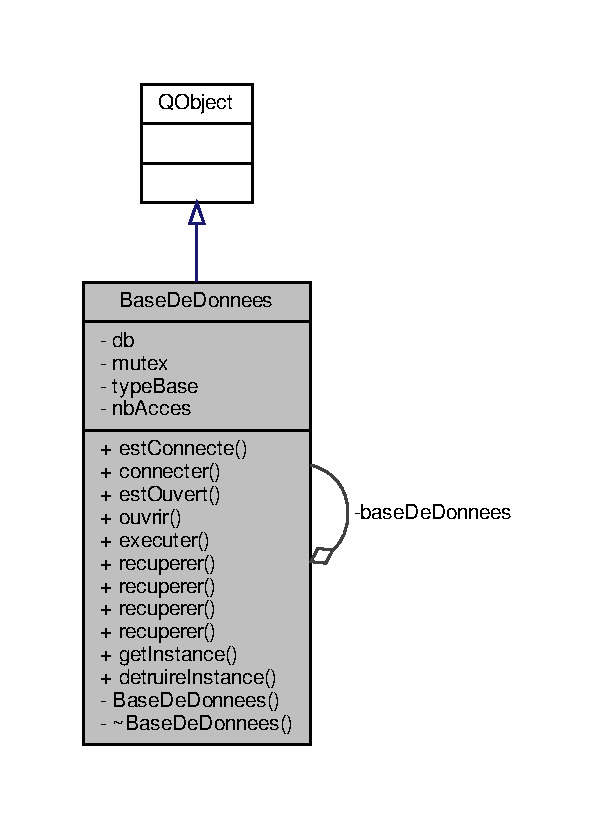
\includegraphics[width=286pt]{class_base_de_donnees__coll__graph}
\end{center}
\end{figure}
\subsubsection*{Fonctions membres publiques}
\begin{DoxyCompactItemize}
\item 
bool \hyperlink{class_base_de_donnees_a00388973f3ec42e5c8e76e7af7e124b2}{est\+Connecte} ()
\item 
bool \hyperlink{class_base_de_donnees_ab2e092285ccc0ee1cce61a1774218561}{connecter} (Q\+String nom\+Base, Q\+String username=\hyperlink{basededonnees_8h_a88b5f5b81fa534553c68802384beff2c}{B\+D\+D\+\_\+\+U\+S\+E\+R\+N\+A\+ME}, Q\+String password=\hyperlink{basededonnees_8h_ae2ded9166ed2553182545e97514c04f7}{B\+D\+D\+\_\+\+P\+A\+S\+S\+W\+O\+RD}, Q\+String serveur=\hyperlink{basededonnees_8h_af06096ec4ec654090fa78ab359d4a0dd}{B\+D\+D\+\_\+\+H\+O\+S\+T\+N\+A\+ME})
\item 
bool \hyperlink{class_base_de_donnees_af9ac332082ffd0dd35e412cefabe5e9c}{est\+Ouvert} ()
\item 
bool \hyperlink{class_base_de_donnees_a7f6a5510b08017b0d99115a84252f186}{ouvrir} (Q\+String fichier\+Base)
\item 
bool \hyperlink{class_base_de_donnees_aa8de5f8f8bb17edc43f5c0ee33712081}{executer} (Q\+String requete)
\item 
bool \hyperlink{class_base_de_donnees_a77539baad389f5acf754cd2cd452403e}{recuperer} (Q\+String requete, Q\+String \&donnees)
\item 
bool \hyperlink{class_base_de_donnees_a2a5c461fa11d404810ae3ebe035d5190}{recuperer} (Q\+String requete, Q\+String\+List \&donnees)
\item 
bool \hyperlink{class_base_de_donnees_af9a76eb2b12df784280c379a4b22af62}{recuperer} (Q\+String requete, Q\+Vector$<$ Q\+String $>$ \&donnees)
\item 
bool \hyperlink{class_base_de_donnees_a68dd0d62ba03b9e8e5aa759d0666cb59}{recuperer} (Q\+String requete, Q\+Vector$<$ Q\+String\+List $>$ \&donnees)
\end{DoxyCompactItemize}
\subsubsection*{Fonctions membres publiques statiques}
\begin{DoxyCompactItemize}
\item 
static \hyperlink{class_base_de_donnees}{Base\+De\+Donnees} $\ast$ \hyperlink{class_base_de_donnees_a80028aa2b6b4fbf30fb2e36357b7d3d3}{get\+Instance} (Q\+String type=\char`\"{}Q\+M\+Y\+S\+QL\char`\"{})
\item 
static void \hyperlink{class_base_de_donnees_a457401c0816b888c77ce915997545f4e}{detruire\+Instance} ()
\end{DoxyCompactItemize}
\subsubsection*{Fonctions membres privées}
\begin{DoxyCompactItemize}
\item 
\hyperlink{class_base_de_donnees_a10dd177f1008f675ab78c2221b2a6750}{Base\+De\+Donnees} (Q\+String type)
\item 
\hyperlink{class_base_de_donnees_a5dc474cdbe003644fb0ca7b8f2ec6b93}{$\sim$\+Base\+De\+Donnees} ()
\end{DoxyCompactItemize}
\subsubsection*{Attributs privés}
\begin{DoxyCompactItemize}
\item 
Q\+Sql\+Database \hyperlink{class_base_de_donnees_a3e738dcf443370c46a541677ab619f06}{db}
\item 
Q\+Mutex \hyperlink{class_base_de_donnees_aa1b4696fac87a740f914aa73739086f2}{mutex}
\end{DoxyCompactItemize}
\subsubsection*{Attributs privés statiques}
\begin{DoxyCompactItemize}
\item 
static \hyperlink{class_base_de_donnees}{Base\+De\+Donnees} $\ast$ \hyperlink{class_base_de_donnees_a822ba0b7cf85b1e48ced8efd3d65e266}{base\+De\+Donnees} = nullptr
\item 
static Q\+String \hyperlink{class_base_de_donnees_ab682b82167f494496a6531bfe522b42b}{type\+Base} = \char`\"{}Q\+M\+Y\+S\+QL\char`\"{}
\item 
static int \hyperlink{class_base_de_donnees_a5099ecb2922bb31d84cd5d4505298a29}{nb\+Acces} = 0
\end{DoxyCompactItemize}


\subsubsection{Documentation des constructeurs et destructeur}
\mbox{\Hypertarget{class_base_de_donnees_a10dd177f1008f675ab78c2221b2a6750}\label{class_base_de_donnees_a10dd177f1008f675ab78c2221b2a6750}} 
\index{Base\+De\+Donnees@{Base\+De\+Donnees}!Base\+De\+Donnees@{Base\+De\+Donnees}}
\index{Base\+De\+Donnees@{Base\+De\+Donnees}!Base\+De\+Donnees@{Base\+De\+Donnees}}
\paragraph{\texorpdfstring{Base\+De\+Donnees()}{BaseDeDonnees()}}
{\footnotesize\ttfamily Base\+De\+Donnees\+::\+Base\+De\+Donnees (\begin{DoxyParamCaption}\item[{Q\+String}]{type }\end{DoxyParamCaption})\hspace{0.3cm}{\ttfamily [private]}}



Références \hyperlink{class_base_de_donnees_a3e738dcf443370c46a541677ab619f06}{db}, et \hyperlink{class_base_de_donnees_ab682b82167f494496a6531bfe522b42b}{type\+Base}.



Référencé par \hyperlink{class_base_de_donnees_a80028aa2b6b4fbf30fb2e36357b7d3d3}{get\+Instance()}.


\begin{DoxyCode}
00023 \{
00024 \textcolor{preprocessor}{    #ifdef DEBUG\_BASEDEDONNEES}
00025     qDebug() << Q\_FUNC\_INFO << type;
00026 \textcolor{preprocessor}{    #endif}
00027     \hyperlink{class_base_de_donnees_a3e738dcf443370c46a541677ab619f06}{db} = QSqlDatabase::addDatabase(type);
00028     \hyperlink{class_base_de_donnees_ab682b82167f494496a6531bfe522b42b}{typeBase} = type;
00029 \}
\end{DoxyCode}
\mbox{\Hypertarget{class_base_de_donnees_a5dc474cdbe003644fb0ca7b8f2ec6b93}\label{class_base_de_donnees_a5dc474cdbe003644fb0ca7b8f2ec6b93}} 
\index{Base\+De\+Donnees@{Base\+De\+Donnees}!````~Base\+De\+Donnees@{$\sim$\+Base\+De\+Donnees}}
\index{````~Base\+De\+Donnees@{$\sim$\+Base\+De\+Donnees}!Base\+De\+Donnees@{Base\+De\+Donnees}}
\paragraph{\texorpdfstring{$\sim$\+Base\+De\+Donnees()}{~BaseDeDonnees()}}
{\footnotesize\ttfamily Base\+De\+Donnees\+::$\sim$\+Base\+De\+Donnees (\begin{DoxyParamCaption}{ }\end{DoxyParamCaption})\hspace{0.3cm}{\ttfamily [private]}}


\begin{DoxyCode}
00032 \{
00033 \textcolor{preprocessor}{    #ifdef DEBUG\_BASEDEDONNEES}
00034     qDebug() << Q\_FUNC\_INFO;
00035 \textcolor{preprocessor}{    #endif}
00036 \}
\end{DoxyCode}


\subsubsection{Documentation des fonctions membres}
\mbox{\Hypertarget{class_base_de_donnees_ab2e092285ccc0ee1cce61a1774218561}\label{class_base_de_donnees_ab2e092285ccc0ee1cce61a1774218561}} 
\index{Base\+De\+Donnees@{Base\+De\+Donnees}!connecter@{connecter}}
\index{connecter@{connecter}!Base\+De\+Donnees@{Base\+De\+Donnees}}
\paragraph{\texorpdfstring{connecter()}{connecter()}}
{\footnotesize\ttfamily bool Base\+De\+Donnees\+::connecter (\begin{DoxyParamCaption}\item[{Q\+String}]{nom\+Base,  }\item[{Q\+String}]{username = {\ttfamily \hyperlink{basededonnees_8h_a88b5f5b81fa534553c68802384beff2c}{B\+D\+D\+\_\+\+U\+S\+E\+R\+N\+A\+ME}},  }\item[{Q\+String}]{password = {\ttfamily \hyperlink{basededonnees_8h_ae2ded9166ed2553182545e97514c04f7}{B\+D\+D\+\_\+\+P\+A\+S\+S\+W\+O\+RD}},  }\item[{Q\+String}]{serveur = {\ttfamily \hyperlink{basededonnees_8h_af06096ec4ec654090fa78ab359d4a0dd}{B\+D\+D\+\_\+\+H\+O\+S\+T\+N\+A\+ME}} }\end{DoxyParamCaption})}



Références \hyperlink{class_base_de_donnees_a3e738dcf443370c46a541677ab619f06}{db}, \hyperlink{class_base_de_donnees_aa1b4696fac87a740f914aa73739086f2}{mutex}, et \hyperlink{class_base_de_donnees_ab682b82167f494496a6531bfe522b42b}{type\+Base}.



Référencé par \hyperlink{class_coureur_af3a5607d96a0960b1666164f6a74d539}{Coureur\+::\+Coureur()}, \hyperlink{class_course_af6317ecab95f8a2eb205b4f91b530992}{Course\+::\+Course()}, \hyperlink{class_gestion_b_d_d_a406bdb9b1714b204fa6fab015baffc27}{Gestion\+B\+D\+D\+::\+Gestion\+B\+D\+D()}, \hyperlink{class_i_h_m_resultats_cross_a94afa0356ebc98e497dfecca3e1bb00b}{I\+H\+M\+Resultats\+Cross\+::\+I\+H\+M\+Resultats\+Cross()}, et \hyperlink{class_resultat_a57e458f7abfc7463786ae9212bf55cd5}{Resultat\+::\+Resultat()}.


\begin{DoxyCode}
00077 \{
00078     \textcolor{keywordflow}{if}(\hyperlink{class_base_de_donnees_ab682b82167f494496a6531bfe522b42b}{typeBase} != \textcolor{stringliteral}{"QMYSQL"})
00079         \textcolor{keywordflow}{return} \textcolor{keyword}{false};
00080     QMutexLocker verrou(&\hyperlink{class_base_de_donnees_aa1b4696fac87a740f914aa73739086f2}{mutex});
00081     \textcolor{keywordflow}{if}(!\hyperlink{class_base_de_donnees_a3e738dcf443370c46a541677ab619f06}{db}.isOpen())
00082     \{
00083        \hyperlink{class_base_de_donnees_a3e738dcf443370c46a541677ab619f06}{db}.setHostName(serveur);
00084        \hyperlink{class_base_de_donnees_a3e738dcf443370c46a541677ab619f06}{db}.setUserName(username);
00085        \hyperlink{class_base_de_donnees_a3e738dcf443370c46a541677ab619f06}{db}.setPassword(password);
00086        \hyperlink{class_base_de_donnees_a3e738dcf443370c46a541677ab619f06}{db}.setDatabaseName(nomBase);
00087 
00088        qDebug() << Q\_FUNC\_INFO << \hyperlink{class_base_de_donnees_a3e738dcf443370c46a541677ab619f06}{db};
00089 \textcolor{preprocessor}{       #ifdef DEBUG\_BASEDEDONNEES}
00090        qDebug() << Q\_FUNC\_INFO;
00091        qDebug() << \textcolor{stringliteral}{"HostName : "} << db.hostName();
00092        qDebug() << \textcolor{stringliteral}{"UserName : "} << db.userName();
00093        qDebug() << \textcolor{stringliteral}{"DatabaseName : "} << db.databaseName();
00094 \textcolor{preprocessor}{       #endif}
00095        \textcolor{keywordflow}{if}(db.open())
00096        \{
00097 \textcolor{preprocessor}{           #ifdef DEBUG\_BASEDEDONNEES}
00098            qDebug() << Q\_FUNC\_INFO << QString::fromUtf8(\textcolor{stringliteral}{"Connexion réussie à %1"}).arg(db.hostName());
00099 \textcolor{preprocessor}{           #endif}
00100            \textcolor{keywordflow}{return} \textcolor{keyword}{true};
00101        \}
00102        \textcolor{keywordflow}{else}
00103        \{
00104            qDebug() << Q\_FUNC\_INFO << QString::fromUtf8(\textcolor{stringliteral}{"Erreur : impossible de se connecter à la base de
       données !"});
00105            QMessageBox::critical(0, QString::fromUtf8(\textcolor{stringliteral}{"BaseDeDonnees"}), QString::fromUtf8(\textcolor{stringliteral}{"Impossible de se
       connecter à la base de données !"}));
00106            \textcolor{keywordflow}{return} \textcolor{keyword}{false};
00107        \}
00108     \}
00109     \textcolor{keywordflow}{else}
00110         \textcolor{keywordflow}{return} \textcolor{keyword}{true};
00111 \}
\end{DoxyCode}
\mbox{\Hypertarget{class_base_de_donnees_a457401c0816b888c77ce915997545f4e}\label{class_base_de_donnees_a457401c0816b888c77ce915997545f4e}} 
\index{Base\+De\+Donnees@{Base\+De\+Donnees}!detruire\+Instance@{detruire\+Instance}}
\index{detruire\+Instance@{detruire\+Instance}!Base\+De\+Donnees@{Base\+De\+Donnees}}
\paragraph{\texorpdfstring{detruire\+Instance()}{detruireInstance()}}
{\footnotesize\ttfamily void Base\+De\+Donnees\+::detruire\+Instance (\begin{DoxyParamCaption}{ }\end{DoxyParamCaption})\hspace{0.3cm}{\ttfamily [static]}}



Références \hyperlink{class_base_de_donnees_a822ba0b7cf85b1e48ced8efd3d65e266}{base\+De\+Donnees}, et \hyperlink{class_base_de_donnees_a5099ecb2922bb31d84cd5d4505298a29}{nb\+Acces}.



Référencé par \hyperlink{class_course_aa9038f2e129526920037dda9e76d69d0}{Course\+::$\sim$\+Course()}, \hyperlink{class_gestion_b_d_d_a4d98c4008182a5749c57c97772b3c303}{Gestion\+B\+D\+D\+::$\sim$\+Gestion\+B\+D\+D()}, \hyperlink{class_i_h_m_chrono_cross_a312f21e1d150096b3f36ba36476907eb}{I\+H\+M\+Chrono\+Cross\+::$\sim$\+I\+H\+M\+Chrono\+Cross()}, \hyperlink{class_i_h_m_gestion_cross_a47cc1d5e80bea3d5e3396a8c16158c45}{I\+H\+M\+Gestion\+Cross\+::$\sim$\+I\+H\+M\+Gestion\+Cross()}, \hyperlink{class_i_h_m_resultats_cross_a62afe926862fddcb340e4a2c57c3cddf}{I\+H\+M\+Resultats\+Cross\+::$\sim$\+I\+H\+M\+Resultats\+Cross()}, et \hyperlink{class_resultat_ae159333a3c5b89b8f307086bac618d7c}{Resultat\+::$\sim$\+Resultat()}.


\begin{DoxyCode}
00052 \{
00053     \textcolor{comment}{// instance ?}
00054     \textcolor{keywordflow}{if}(\hyperlink{class_base_de_donnees_a822ba0b7cf85b1e48ced8efd3d65e266}{baseDeDonnees} != \textcolor{keyword}{nullptr})
00055     \{
00056         \textcolor{keywordflow}{if}(\hyperlink{class_base_de_donnees_a5099ecb2922bb31d84cd5d4505298a29}{nbAcces} > 0)
00057             \hyperlink{class_base_de_donnees_a5099ecb2922bb31d84cd5d4505298a29}{nbAcces}--;
00058 \textcolor{preprocessor}{        #ifdef DEBUG\_BASEDEDONNEES}
00059         qDebug() << Q\_FUNC\_INFO << \textcolor{stringliteral}{"nbAcces restants"} << \hyperlink{class_base_de_donnees_a5099ecb2922bb31d84cd5d4505298a29}{nbAcces};
00060 \textcolor{preprocessor}{        #endif}
00061         \textcolor{comment}{// dernier ?}
00062         \textcolor{keywordflow}{if}(nbAcces == 0)
00063         \{
00064             \textcolor{keyword}{delete} \hyperlink{class_base_de_donnees_a822ba0b7cf85b1e48ced8efd3d65e266}{baseDeDonnees};
00065             \hyperlink{class_base_de_donnees_a822ba0b7cf85b1e48ced8efd3d65e266}{baseDeDonnees} = \textcolor{keyword}{nullptr};
00066         \}
00067     \}
00068 \}
\end{DoxyCode}
\mbox{\Hypertarget{class_base_de_donnees_a00388973f3ec42e5c8e76e7af7e124b2}\label{class_base_de_donnees_a00388973f3ec42e5c8e76e7af7e124b2}} 
\index{Base\+De\+Donnees@{Base\+De\+Donnees}!est\+Connecte@{est\+Connecte}}
\index{est\+Connecte@{est\+Connecte}!Base\+De\+Donnees@{Base\+De\+Donnees}}
\paragraph{\texorpdfstring{est\+Connecte()}{estConnecte()}}
{\footnotesize\ttfamily bool Base\+De\+Donnees\+::est\+Connecte (\begin{DoxyParamCaption}{ }\end{DoxyParamCaption})}



Références \hyperlink{class_base_de_donnees_a3e738dcf443370c46a541677ab619f06}{db}, et \hyperlink{class_base_de_donnees_aa1b4696fac87a740f914aa73739086f2}{mutex}.



Référencé par \hyperlink{class_coureur_af3a5607d96a0960b1666164f6a74d539}{Coureur\+::\+Coureur()}, \hyperlink{class_course_af6317ecab95f8a2eb205b4f91b530992}{Course\+::\+Course()}, \hyperlink{class_gestion_b_d_d_a406bdb9b1714b204fa6fab015baffc27}{Gestion\+B\+D\+D\+::\+Gestion\+B\+D\+D()}, \hyperlink{class_i_h_m_resultats_cross_a94afa0356ebc98e497dfecca3e1bb00b}{I\+H\+M\+Resultats\+Cross\+::\+I\+H\+M\+Resultats\+Cross()}, et \hyperlink{class_resultat_a57e458f7abfc7463786ae9212bf55cd5}{Resultat\+::\+Resultat()}.


\begin{DoxyCode}
00071 \{
00072     QMutexLocker verrou(&\hyperlink{class_base_de_donnees_aa1b4696fac87a740f914aa73739086f2}{mutex});
00073     \textcolor{keywordflow}{return} \hyperlink{class_base_de_donnees_a3e738dcf443370c46a541677ab619f06}{db}.isOpen();
00074 \}
\end{DoxyCode}
\mbox{\Hypertarget{class_base_de_donnees_af9ac332082ffd0dd35e412cefabe5e9c}\label{class_base_de_donnees_af9ac332082ffd0dd35e412cefabe5e9c}} 
\index{Base\+De\+Donnees@{Base\+De\+Donnees}!est\+Ouvert@{est\+Ouvert}}
\index{est\+Ouvert@{est\+Ouvert}!Base\+De\+Donnees@{Base\+De\+Donnees}}
\paragraph{\texorpdfstring{est\+Ouvert()}{estOuvert()}}
{\footnotesize\ttfamily bool Base\+De\+Donnees\+::est\+Ouvert (\begin{DoxyParamCaption}{ }\end{DoxyParamCaption})}



Références \hyperlink{class_base_de_donnees_a3e738dcf443370c46a541677ab619f06}{db}, et \hyperlink{class_base_de_donnees_aa1b4696fac87a740f914aa73739086f2}{mutex}.


\begin{DoxyCode}
00114 \{
00115     QMutexLocker verrou(&\hyperlink{class_base_de_donnees_aa1b4696fac87a740f914aa73739086f2}{mutex});
00116     \textcolor{keywordflow}{return} \hyperlink{class_base_de_donnees_a3e738dcf443370c46a541677ab619f06}{db}.isOpen();
00117 \}
\end{DoxyCode}
\mbox{\Hypertarget{class_base_de_donnees_aa8de5f8f8bb17edc43f5c0ee33712081}\label{class_base_de_donnees_aa8de5f8f8bb17edc43f5c0ee33712081}} 
\index{Base\+De\+Donnees@{Base\+De\+Donnees}!executer@{executer}}
\index{executer@{executer}!Base\+De\+Donnees@{Base\+De\+Donnees}}
\paragraph{\texorpdfstring{executer()}{executer()}}
{\footnotesize\ttfamily bool Base\+De\+Donnees\+::executer (\begin{DoxyParamCaption}\item[{Q\+String}]{requete }\end{DoxyParamCaption})}



Références \hyperlink{class_base_de_donnees_a3e738dcf443370c46a541677ab619f06}{db}, et \hyperlink{class_base_de_donnees_aa1b4696fac87a740f914aa73739086f2}{mutex}.



Référencé par \hyperlink{class_course_ac99042bf8b20e8d3a54e72c8a80f7ee7}{Course\+::ajoute\+Arrivee\+B\+D\+D()}, \hyperlink{class_gestion_b_d_d_ae71561eea6d1163ff067f079ccc6d169}{Gestion\+B\+D\+D\+::ajouter\+Nouveau\+Coureur()}, \hyperlink{class_gestion_b_d_d_a71391d5419969b52cd999463b5326599}{Gestion\+B\+D\+D\+::ajouter\+Nouvel\+Inscrit()}, \hyperlink{class_gestion_b_d_d_afad096d7e405d35a818d4858ee34df61}{Gestion\+B\+D\+D\+::modifier\+Coureur()}, \hyperlink{class_course_a3ebcde1fa443cb20d71fb98af4d0c418}{Course\+::set\+Etat()}, et \hyperlink{class_gestion_b_d_d_afe47ec92274b7998131c5d4e6551d177}{Gestion\+B\+D\+D\+::supprimer\+Coureur()}.


\begin{DoxyCode}
00152 \{
00153     QMutexLocker verrou(&\hyperlink{class_base_de_donnees_aa1b4696fac87a740f914aa73739086f2}{mutex});
00154     QSqlQuery r;
00155     \textcolor{keywordtype}{bool} retour;
00156 
00157     \textcolor{keywordflow}{if}(\hyperlink{class_base_de_donnees_a3e738dcf443370c46a541677ab619f06}{db}.isOpen())
00158     \{
00159         \textcolor{keywordflow}{if}(requete.contains(\textcolor{stringliteral}{"UPDATE"}) || requete.contains(\textcolor{stringliteral}{"INSERT"}) || requete.contains(\textcolor{stringliteral}{"DELETE"}))
00160         \{
00161             retour = r.exec(requete);
00162 \textcolor{preprocessor}{            #ifdef DEBUG\_BASEDEDONNEES}
00163             qDebug() << Q\_FUNC\_INFO << QString::fromUtf8(\textcolor{stringliteral}{"Retour %1 pour la requete : %2"}).arg(
      QString::number(retour)).arg(requete);
00164 \textcolor{preprocessor}{            #endif}
00165             \textcolor{keywordflow}{if}(retour)
00166             \{
00167                 \textcolor{keywordflow}{return} \textcolor{keyword}{true};
00168             \}
00169             \textcolor{keywordflow}{else}
00170             \{
00171                 qDebug() << Q\_FUNC\_INFO << QString::fromUtf8(\textcolor{stringliteral}{"Erreur : %1 pour la requête %2"}).arg(r.
      lastError().text()).arg(requete);
00172                 \textcolor{keywordflow}{return} \textcolor{keyword}{false};
00173             \}
00174         \}
00175         \textcolor{keywordflow}{else}
00176         \{
00177             qDebug() << Q\_FUNC\_INFO << QString::fromUtf8(\textcolor{stringliteral}{"Erreur : requête %1 non autorisée !"}).arg(requete
      );
00178             \textcolor{keywordflow}{return} \textcolor{keyword}{false};
00179         \}
00180     \}
00181     \textcolor{keywordflow}{else}
00182         \textcolor{keywordflow}{return} \textcolor{keyword}{false};
00183 
00184 \}
\end{DoxyCode}
\mbox{\Hypertarget{class_base_de_donnees_a80028aa2b6b4fbf30fb2e36357b7d3d3}\label{class_base_de_donnees_a80028aa2b6b4fbf30fb2e36357b7d3d3}} 
\index{Base\+De\+Donnees@{Base\+De\+Donnees}!get\+Instance@{get\+Instance}}
\index{get\+Instance@{get\+Instance}!Base\+De\+Donnees@{Base\+De\+Donnees}}
\paragraph{\texorpdfstring{get\+Instance()}{getInstance()}}
{\footnotesize\ttfamily \hyperlink{class_base_de_donnees}{Base\+De\+Donnees} $\ast$ Base\+De\+Donnees\+::get\+Instance (\begin{DoxyParamCaption}\item[{Q\+String}]{type = {\ttfamily \char`\"{}QMYSQL\char`\"{}} }\end{DoxyParamCaption})\hspace{0.3cm}{\ttfamily [static]}}



Références \hyperlink{class_base_de_donnees_a10dd177f1008f675ab78c2221b2a6750}{Base\+De\+Donnees()}, \hyperlink{class_base_de_donnees_a822ba0b7cf85b1e48ced8efd3d65e266}{base\+De\+Donnees}, et \hyperlink{class_base_de_donnees_a5099ecb2922bb31d84cd5d4505298a29}{nb\+Acces}.



Référencé par \hyperlink{class_coureur_af3a5607d96a0960b1666164f6a74d539}{Coureur\+::\+Coureur()}, \hyperlink{class_course_af6317ecab95f8a2eb205b4f91b530992}{Course\+::\+Course()}, \hyperlink{class_gestion_b_d_d_a406bdb9b1714b204fa6fab015baffc27}{Gestion\+B\+D\+D\+::\+Gestion\+B\+D\+D()}, \hyperlink{class_i_h_m_resultats_cross_a94afa0356ebc98e497dfecca3e1bb00b}{I\+H\+M\+Resultats\+Cross\+::\+I\+H\+M\+Resultats\+Cross()}, et \hyperlink{class_resultat_a57e458f7abfc7463786ae9212bf55cd5}{Resultat\+::\+Resultat()}.


\begin{DoxyCode}
00039 \{
00040     \textcolor{keywordflow}{if}(\hyperlink{class_base_de_donnees_a822ba0b7cf85b1e48ced8efd3d65e266}{baseDeDonnees} == \textcolor{keyword}{nullptr})
00041         \hyperlink{class_base_de_donnees_a822ba0b7cf85b1e48ced8efd3d65e266}{baseDeDonnees} = \textcolor{keyword}{new} \hyperlink{class_base_de_donnees_a10dd177f1008f675ab78c2221b2a6750}{BaseDeDonnees}(type);
00042 
00043     \hyperlink{class_base_de_donnees_a5099ecb2922bb31d84cd5d4505298a29}{nbAcces}++;
00044 \textcolor{preprocessor}{    #ifdef DEBUG\_BASEDEDONNEES}
00045     qDebug() << Q\_FUNC\_INFO << \textcolor{stringliteral}{"nbAcces"} << \hyperlink{class_base_de_donnees_a5099ecb2922bb31d84cd5d4505298a29}{nbAcces};
00046 \textcolor{preprocessor}{    #endif}
00047 
00048     \textcolor{keywordflow}{return} \hyperlink{class_base_de_donnees_a822ba0b7cf85b1e48ced8efd3d65e266}{baseDeDonnees};
00049 \}
\end{DoxyCode}
\mbox{\Hypertarget{class_base_de_donnees_a7f6a5510b08017b0d99115a84252f186}\label{class_base_de_donnees_a7f6a5510b08017b0d99115a84252f186}} 
\index{Base\+De\+Donnees@{Base\+De\+Donnees}!ouvrir@{ouvrir}}
\index{ouvrir@{ouvrir}!Base\+De\+Donnees@{Base\+De\+Donnees}}
\paragraph{\texorpdfstring{ouvrir()}{ouvrir()}}
{\footnotesize\ttfamily bool Base\+De\+Donnees\+::ouvrir (\begin{DoxyParamCaption}\item[{Q\+String}]{fichier\+Base }\end{DoxyParamCaption})}



Références \hyperlink{class_base_de_donnees_a3e738dcf443370c46a541677ab619f06}{db}, \hyperlink{class_base_de_donnees_aa1b4696fac87a740f914aa73739086f2}{mutex}, et \hyperlink{class_base_de_donnees_ab682b82167f494496a6531bfe522b42b}{type\+Base}.


\begin{DoxyCode}
00120 \{
00121     \textcolor{keywordflow}{if}(\hyperlink{class_base_de_donnees_ab682b82167f494496a6531bfe522b42b}{typeBase} != \textcolor{stringliteral}{"QSQLITE"})
00122         \textcolor{keywordflow}{return} \textcolor{keyword}{false};
00123     QMutexLocker verrou(&\hyperlink{class_base_de_donnees_aa1b4696fac87a740f914aa73739086f2}{mutex});
00124     \textcolor{keywordflow}{if}(!\hyperlink{class_base_de_donnees_a3e738dcf443370c46a541677ab619f06}{db}.isOpen())
00125     \{
00126        \hyperlink{class_base_de_donnees_a3e738dcf443370c46a541677ab619f06}{db}.setDatabaseName(fichierBase);
00127 
00128 \textcolor{preprocessor}{       #ifdef DEBUG\_BASEDEDONNEES}
00129        qDebug() << Q\_FUNC\_INFO << \hyperlink{class_base_de_donnees_a3e738dcf443370c46a541677ab619f06}{db}.databaseName();       
00130 \textcolor{preprocessor}{       #endif}
00131        \textcolor{keywordflow}{if}(\hyperlink{class_base_de_donnees_a3e738dcf443370c46a541677ab619f06}{db}.open())
00132        \{
00133 \textcolor{preprocessor}{           #ifdef DEBUG\_BASEDEDONNEES}
00134            qDebug() << Q\_FUNC\_INFO << QString::fromUtf8(\textcolor{stringliteral}{"Ouvertir réussie à %1"}).arg(
      \hyperlink{class_base_de_donnees_a3e738dcf443370c46a541677ab619f06}{db}.databaseName());
00135 \textcolor{preprocessor}{           #endif}
00136 
00137            \textcolor{keywordflow}{return} \textcolor{keyword}{true};
00138        \}
00139        \textcolor{keywordflow}{else}
00140        \{
00141            qDebug() << Q\_FUNC\_INFO << QString::fromUtf8(\textcolor{stringliteral}{"Erreur : impossible d'ouvrir la base de données !"}
      );
00142            QMessageBox::critical(0, QString::fromUtf8(\textcolor{stringliteral}{"BaseDeDonnees"}), QString::fromUtf8(\textcolor{stringliteral}{"Impossible
       d'ouvrir la base de données !"}));
00143            \textcolor{keywordflow}{return} \textcolor{keyword}{false};
00144        \}
00145     \}
00146     \textcolor{keywordflow}{else}
00147         \textcolor{keywordflow}{return} \textcolor{keyword}{true};
00148 \}
\end{DoxyCode}
\mbox{\Hypertarget{class_base_de_donnees_a77539baad389f5acf754cd2cd452403e}\label{class_base_de_donnees_a77539baad389f5acf754cd2cd452403e}} 
\index{Base\+De\+Donnees@{Base\+De\+Donnees}!recuperer@{recuperer}}
\index{recuperer@{recuperer}!Base\+De\+Donnees@{Base\+De\+Donnees}}
\paragraph{\texorpdfstring{recuperer()}{recuperer()}\hspace{0.1cm}{\footnotesize\ttfamily [1/4]}}
{\footnotesize\ttfamily bool Base\+De\+Donnees\+::recuperer (\begin{DoxyParamCaption}\item[{Q\+String}]{requete,  }\item[{Q\+String \&}]{donnees }\end{DoxyParamCaption})}



Références \hyperlink{class_base_de_donnees_a3e738dcf443370c46a541677ab619f06}{db}, et \hyperlink{class_base_de_donnees_aa1b4696fac87a740f914aa73739086f2}{mutex}.



Référencé par \hyperlink{class_course_ac99042bf8b20e8d3a54e72c8a80f7ee7}{Course\+::ajoute\+Arrivee\+B\+D\+D()}, \hyperlink{class_gestion_b_d_d_ae71561eea6d1163ff067f079ccc6d169}{Gestion\+B\+D\+D\+::ajouter\+Nouveau\+Coureur()}, \hyperlink{class_gestion_b_d_d_a71391d5419969b52cd999463b5326599}{Gestion\+B\+D\+D\+::ajouter\+Nouvel\+Inscrit()}, \hyperlink{class_course_af20fcd6d6eb2dfbd3b0f12e273f12b27}{Course\+::get\+Distance()}, \hyperlink{class_course_afc21f8195edd50c9fd266cff0c401b7c}{Course\+::get\+Heure()}, \hyperlink{class_course_a7ba5d2c9865065e95f49a24fbeec7857}{Course\+::get\+Information\+Coureur()}, \hyperlink{class_course_ae5e74946d973166ad3000e38600acf20}{Course\+::get\+Liste\+Courses()}, \hyperlink{class_course_a0d995ef72152208e02eb3b10315dfabb}{Course\+::get\+Liste\+Manifestations()}, \hyperlink{class_course_ad8dd87e7f299bc938f40423f28c837e8}{Course\+::get\+Nb\+Arrivee()}, \hyperlink{class_course_ad0ff4153f1e02826d551f478f95ad260}{Course\+::get\+Nb\+Inscrit()}, \hyperlink{class_course_a7b4485a0b38bc3b908131962b705d880}{Course\+::get\+Nom\+Course()}, \hyperlink{class_gestion_b_d_d_afad096d7e405d35a818d4858ee34df61}{Gestion\+B\+D\+D\+::modifier\+Coureur()}, \hyperlink{class_gestion_b_d_d_a76ab3e307ad9005dcdb2781fc77fc5c8}{Gestion\+B\+D\+D\+::recuperer\+Categories\+Creation()}, \hyperlink{class_gestion_b_d_d_ad7b0117ad5d55f21e6f00858038f4a85}{Gestion\+B\+D\+D\+::recuperer\+Catergorie\+Coureur()}, \hyperlink{class_gestion_b_d_d_a0e90b16b2e330de9cc80f72f0d648e5d}{Gestion\+B\+D\+D\+::recuperer\+Classe\+Coureur()}, \hyperlink{class_gestion_b_d_d_a38d728d644f23048f1a6d3e6d4656764}{Gestion\+B\+D\+D\+::recuperer\+Classes\+Creation()}, \hyperlink{class_gestion_b_d_d_a0a2fa02b90974684658937fbfb55bf0a}{Gestion\+B\+D\+D\+::recuperer\+Information()}, \hyperlink{class_gestion_b_d_d_a09b547cb065256acd269c64e273c93fd}{Gestion\+B\+D\+D\+::recuperer\+Liste\+Coureurs\+Inscrit()}, \hyperlink{class_gestion_b_d_d_ac35de40fd5860b3130f71788ecaa5ef3}{Gestion\+B\+D\+D\+::recuperer\+Liste\+Courses\+Gestion()}, \hyperlink{class_gestion_b_d_d_a59ef29e28993c64aa4d5a8c42a8fb08d}{Gestion\+B\+D\+D\+::recuperer\+Liste\+Courses\+Inscription()}, \hyperlink{class_gestion_b_d_d_a6c1ab5e51fbd6c92bb096badbeac0df5}{Gestion\+B\+D\+D\+::recuperer\+Liste\+Manifestations\+Inscription()}, \hyperlink{class_gestion_b_d_d_a2b44ebc5bf5b1a7babde6512817a85b4}{Gestion\+B\+D\+D\+::recuperer\+Table\+B\+D\+D()}, \hyperlink{class_course_a36cf16c971841431947b6fbe2b3f3d27}{Course\+::set\+Id\+Course()}, \hyperlink{class_gestion_b_d_d_afe47ec92274b7998131c5d4e6551d177}{Gestion\+B\+D\+D\+::supprimer\+Coureur()}, \hyperlink{class_gestion_b_d_d_a1a39bbc7bfcb60d286363b9d2dd7f88b}{Gestion\+B\+D\+D\+::verifier\+Dossard()}, \hyperlink{class_course_a6cb3ede6a11e4813f95be92f4459a3c2}{Course\+::verifier\+Dossard()}, et \hyperlink{class_gestion_b_d_d_abfd3cfb9553a83aafd86c3149869d6c0}{Gestion\+B\+D\+D\+::verifier\+Information()}.


\begin{DoxyCode}
00190 \{
00191     QMutexLocker verrou(&\hyperlink{class_base_de_donnees_aa1b4696fac87a740f914aa73739086f2}{mutex});
00192     QSqlQuery r;
00193     \textcolor{keywordtype}{bool} retour;
00194 
00195     \textcolor{keywordflow}{if}(\hyperlink{class_base_de_donnees_a3e738dcf443370c46a541677ab619f06}{db}.isOpen())
00196     \{
00197         \textcolor{keywordflow}{if}(requete.contains(\textcolor{stringliteral}{"SELECT"}))
00198         \{
00199             retour = r.exec(requete);
00200 \textcolor{preprocessor}{            #ifdef DEBUG\_BASEDEDONNEES}
00201             qDebug() << Q\_FUNC\_INFO << QString::fromUtf8(\textcolor{stringliteral}{"Retour %1 pour la requete : %2"}).arg(
      QString::number(retour)).arg(requete);
00202 \textcolor{preprocessor}{            #endif}
00203             \textcolor{keywordflow}{if}(retour)
00204             \{
00205                 \textcolor{comment}{// on se positionne sur l'enregistrement}
00206                 r.first();
00207 
00208                 \textcolor{comment}{// on vérifie l'état de l'enregistrement retourné}
00209                 \textcolor{keywordflow}{if}(!r.isValid())
00210                 \{
00211 \textcolor{preprocessor}{                    #ifdef DEBUG\_BASEDEDONNEES}
00212                     qDebug() << Q\_FUNC\_INFO << QString::fromUtf8(\textcolor{stringliteral}{"Résultat non valide !"});
00213 \textcolor{preprocessor}{                    #endif}
00214                     \textcolor{keywordflow}{return} \textcolor{keyword}{false};
00215                 \}
00216 
00217                 \textcolor{comment}{// on récupère sous forme de QString la valeur du champ}
00218                 \textcolor{keywordflow}{if}(r.isNull(0))
00219                 \{
00220 \textcolor{preprocessor}{                    #ifdef DEBUG\_BASEDEDONNEES}
00221                     qDebug() << Q\_FUNC\_INFO << QString::fromUtf8(\textcolor{stringliteral}{"Aucun résultat !"});
00222 \textcolor{preprocessor}{                    #endif}
00223                     \textcolor{keywordflow}{return} \textcolor{keyword}{false};
00224                 \}
00225                 donnees = r.value(0).toString();
00226 \textcolor{preprocessor}{                #ifdef DEBUG\_BASEDEDONNEES}
00227                 qDebug() << Q\_FUNC\_INFO << \textcolor{stringliteral}{"Enregistrement -> "} << donnees;
00228 \textcolor{preprocessor}{                #endif}
00229                 \textcolor{keywordflow}{return} \textcolor{keyword}{true};
00230             \}
00231             \textcolor{keywordflow}{else}
00232             \{
00233                 qDebug() << Q\_FUNC\_INFO << QString::fromUtf8(\textcolor{stringliteral}{"Erreur : %1 pour la requête %2"}).arg(r.
      lastError().text()).arg(requete);
00234                 \textcolor{keywordflow}{return} \textcolor{keyword}{false};
00235             \}
00236         \}
00237         \textcolor{keywordflow}{else}
00238         \{
00239             qDebug() << Q\_FUNC\_INFO << QString::fromUtf8(\textcolor{stringliteral}{"Erreur : requête %1 non autorisée !"}).arg(requete
      );
00240             \textcolor{keywordflow}{return} \textcolor{keyword}{false};
00241         \}
00242     \}
00243     \textcolor{keywordflow}{else}
00244         \textcolor{keywordflow}{return} \textcolor{keyword}{false};
00245 \}
\end{DoxyCode}
\mbox{\Hypertarget{class_base_de_donnees_a2a5c461fa11d404810ae3ebe035d5190}\label{class_base_de_donnees_a2a5c461fa11d404810ae3ebe035d5190}} 
\index{Base\+De\+Donnees@{Base\+De\+Donnees}!recuperer@{recuperer}}
\index{recuperer@{recuperer}!Base\+De\+Donnees@{Base\+De\+Donnees}}
\paragraph{\texorpdfstring{recuperer()}{recuperer()}\hspace{0.1cm}{\footnotesize\ttfamily [2/4]}}
{\footnotesize\ttfamily bool Base\+De\+Donnees\+::recuperer (\begin{DoxyParamCaption}\item[{Q\+String}]{requete,  }\item[{Q\+String\+List \&}]{donnees }\end{DoxyParamCaption})}



Références \hyperlink{class_base_de_donnees_a3e738dcf443370c46a541677ab619f06}{db}, et \hyperlink{class_base_de_donnees_aa1b4696fac87a740f914aa73739086f2}{mutex}.


\begin{DoxyCode}
00251 \{
00252     QMutexLocker verrou(&\hyperlink{class_base_de_donnees_aa1b4696fac87a740f914aa73739086f2}{mutex});
00253     QSqlQuery r;
00254     \textcolor{keywordtype}{bool} retour;
00255 
00256     \textcolor{keywordflow}{if}(\hyperlink{class_base_de_donnees_a3e738dcf443370c46a541677ab619f06}{db}.isOpen())
00257     \{
00258         \textcolor{keywordflow}{if}(requete.contains(\textcolor{stringliteral}{"SELECT"}))
00259         \{
00260             retour = r.exec(requete);
00261 \textcolor{preprocessor}{            #ifdef DEBUG\_BASEDEDONNEES}
00262             qDebug() << QString::fromUtf8(\textcolor{stringliteral}{"<BaseDeDonnees::recuperer(QString, QStringList)> retour %1 pour
       la requete : %2"}).arg(QString::number(retour)).arg(requete);
00263 \textcolor{preprocessor}{            #endif}
00264             \textcolor{keywordflow}{if}(retour)
00265             \{
00266                 \textcolor{comment}{// on se positionne sur l'enregistrement}
00267                 r.first();
00268 
00269                 \textcolor{comment}{// on vérifie l'état de l'enregistrement retourné}
00270                 \textcolor{keywordflow}{if}(!r.isValid())
00271                 \{
00272 \textcolor{preprocessor}{                    #ifdef DEBUG\_BASEDEDONNEES}
00273                     qDebug() << Q\_FUNC\_INFO << QString::fromUtf8(\textcolor{stringliteral}{"Résultat non valide !"});
00274 \textcolor{preprocessor}{                    #endif}
00275                     \textcolor{keywordflow}{return} \textcolor{keyword}{false};
00276                 \}
00277 
00278                 \textcolor{comment}{// on récupère sous forme de QString la valeur de tous les champs sélectionnés}
00279                 \textcolor{comment}{// et on les stocke dans une liste de QString}
00280                 \textcolor{keywordflow}{for}(\textcolor{keywordtype}{int} i=0;i<r.record().count();i++)
00281                     \textcolor{keywordflow}{if}(!r.isNull(i))
00282                         donnees << r.value(i).toString();
00283 \textcolor{preprocessor}{                #ifdef DEBUG\_BASEDEDONNEES}
00284                 qDebug() << Q\_FUNC\_INFO << \textcolor{stringliteral}{"Enregistrement -> "} << donnees;
00285 \textcolor{preprocessor}{                #endif}
00286                 \textcolor{keywordflow}{return} \textcolor{keyword}{true};
00287             \}
00288             \textcolor{keywordflow}{else}
00289             \{
00290                 qDebug() << Q\_FUNC\_INFO << QString::fromUtf8(\textcolor{stringliteral}{"Erreur : %1 pour la requête %2"}).arg(r.
      lastError().text()).arg(requete);
00291                 \textcolor{keywordflow}{return} \textcolor{keyword}{false};
00292             \}
00293         \}
00294         \textcolor{keywordflow}{else}
00295         \{
00296             qDebug() << Q\_FUNC\_INFO << QString::fromUtf8(\textcolor{stringliteral}{"Erreur : requête %1 non autorisée !"}).arg(requete
      );
00297             \textcolor{keywordflow}{return} \textcolor{keyword}{false};
00298         \}
00299     \}
00300     \textcolor{keywordflow}{else}
00301         \textcolor{keywordflow}{return} \textcolor{keyword}{false};
00302 \}
\end{DoxyCode}
\mbox{\Hypertarget{class_base_de_donnees_af9a76eb2b12df784280c379a4b22af62}\label{class_base_de_donnees_af9a76eb2b12df784280c379a4b22af62}} 
\index{Base\+De\+Donnees@{Base\+De\+Donnees}!recuperer@{recuperer}}
\index{recuperer@{recuperer}!Base\+De\+Donnees@{Base\+De\+Donnees}}
\paragraph{\texorpdfstring{recuperer()}{recuperer()}\hspace{0.1cm}{\footnotesize\ttfamily [3/4]}}
{\footnotesize\ttfamily bool Base\+De\+Donnees\+::recuperer (\begin{DoxyParamCaption}\item[{Q\+String}]{requete,  }\item[{Q\+Vector$<$ Q\+String $>$ \&}]{donnees }\end{DoxyParamCaption})}



Références \hyperlink{class_base_de_donnees_a3e738dcf443370c46a541677ab619f06}{db}, et \hyperlink{class_base_de_donnees_aa1b4696fac87a740f914aa73739086f2}{mutex}.


\begin{DoxyCode}
00308 \{
00309     QMutexLocker verrou(&\hyperlink{class_base_de_donnees_aa1b4696fac87a740f914aa73739086f2}{mutex});
00310     QSqlQuery r;
00311     \textcolor{keywordtype}{bool} retour;
00312     QString data;
00313 
00314     \textcolor{keywordflow}{if}(\hyperlink{class_base_de_donnees_a3e738dcf443370c46a541677ab619f06}{db}.isOpen())
00315     \{
00316         \textcolor{keywordflow}{if}(requete.contains(\textcolor{stringliteral}{"SELECT"}))
00317         \{
00318             retour = r.exec(requete);
00319 \textcolor{preprocessor}{            #ifdef DEBUG\_BASEDEDONNEES}
00320             qDebug() << Q\_FUNC\_INFO << QString::fromUtf8(\textcolor{stringliteral}{"Retour %1 pour la requete : %2"}).arg(
      QString::number(retour)).arg(requete);
00321 \textcolor{preprocessor}{            #endif}
00322             \textcolor{keywordflow}{if}(retour)
00323             \{
00324                 \textcolor{comment}{// pour chaque enregistrement}
00325                 \textcolor{keywordflow}{while} ( r.next() )
00326                 \{
00327                     \textcolor{comment}{// on récupère sous forme de QString la valeur du champs sélectionné}
00328                     data = r.value(0).toString();
00329 
00330 \textcolor{preprocessor}{                    #ifdef DEBUG\_BASEDEDONNEES}
00331                     \textcolor{comment}{//qDebug() << Q\_FUNC\_INFO << "Enregistrement -> " << data;}
00332 \textcolor{preprocessor}{                    #endif}
00333 
00334                     \textcolor{comment}{// on stocke l'enregistrement dans le QVector}
00335                     donnees.push\_back(data);
00336                 \}
00337 \textcolor{preprocessor}{                #ifdef DEBUG\_BASEDEDONNEES}
00338                 qDebug() << Q\_FUNC\_INFO << \textcolor{stringliteral}{"Enregistrement -> "} << donnees;
00339 \textcolor{preprocessor}{                #endif}
00340                 \textcolor{keywordflow}{return} \textcolor{keyword}{true};
00341             \}
00342             \textcolor{keywordflow}{else}
00343             \{
00344                 qDebug() << Q\_FUNC\_INFO << QString::fromUtf8(\textcolor{stringliteral}{"Erreur : %1 pour la requête %2"}).arg(r.
      lastError().text()).arg(requete);
00345                 \textcolor{keywordflow}{return} \textcolor{keyword}{false};
00346             \}
00347         \}
00348         \textcolor{keywordflow}{else}
00349         \{
00350             qDebug() << Q\_FUNC\_INFO << QString::fromUtf8(\textcolor{stringliteral}{"Erreur : requête %1 non autorisée !"}).arg(requete
      );
00351             \textcolor{keywordflow}{return} \textcolor{keyword}{false};
00352         \}
00353     \}
00354     \textcolor{keywordflow}{else}
00355         \textcolor{keywordflow}{return} \textcolor{keyword}{false};
00356 \}
\end{DoxyCode}
\mbox{\Hypertarget{class_base_de_donnees_a68dd0d62ba03b9e8e5aa759d0666cb59}\label{class_base_de_donnees_a68dd0d62ba03b9e8e5aa759d0666cb59}} 
\index{Base\+De\+Donnees@{Base\+De\+Donnees}!recuperer@{recuperer}}
\index{recuperer@{recuperer}!Base\+De\+Donnees@{Base\+De\+Donnees}}
\paragraph{\texorpdfstring{recuperer()}{recuperer()}\hspace{0.1cm}{\footnotesize\ttfamily [4/4]}}
{\footnotesize\ttfamily bool Base\+De\+Donnees\+::recuperer (\begin{DoxyParamCaption}\item[{Q\+String}]{requete,  }\item[{Q\+Vector$<$ Q\+String\+List $>$ \&}]{donnees }\end{DoxyParamCaption})}



Références \hyperlink{class_base_de_donnees_a3e738dcf443370c46a541677ab619f06}{db}, et \hyperlink{class_base_de_donnees_aa1b4696fac87a740f914aa73739086f2}{mutex}.


\begin{DoxyCode}
00362 \{
00363     QMutexLocker verrou(&\hyperlink{class_base_de_donnees_aa1b4696fac87a740f914aa73739086f2}{mutex});
00364     QSqlQuery r;
00365     \textcolor{keywordtype}{bool} retour;
00366     QStringList data;
00367 
00368     \textcolor{keywordflow}{if}(\hyperlink{class_base_de_donnees_a3e738dcf443370c46a541677ab619f06}{db}.isOpen())
00369     \{
00370         \textcolor{keywordflow}{if}(requete.contains(\textcolor{stringliteral}{"SELECT"}))
00371         \{
00372             retour = r.exec(requete);
00373 \textcolor{preprocessor}{            #ifdef DEBUG\_BASEDEDONNEES}
00374             qDebug() << Q\_FUNC\_INFO << QString::fromUtf8(\textcolor{stringliteral}{"Retour %1 pour la requete : %2"}).arg(
      QString::number(retour)).arg(requete);
00375 \textcolor{preprocessor}{            #endif}
00376             \textcolor{keywordflow}{if}(retour)
00377             \{
00378                 \textcolor{comment}{// pour chaque enregistrement}
00379                 \textcolor{keywordflow}{while} ( r.next() )
00380                 \{
00381                     \textcolor{comment}{// on récupère sous forme de QString la valeur de tous les champs sélectionnés}
00382                     \textcolor{comment}{// et on les stocke dans une liste de QString}
00383                     \textcolor{keywordflow}{for}(\textcolor{keywordtype}{int} i=0;i<r.record().count();i++)
00384                         data << r.value(i).toString();
00385 
00386 \textcolor{preprocessor}{                    #ifdef DEBUG\_BASEDEDONNEES}
00387                     \textcolor{comment}{//qDebug() << Q\_FUNC\_INFO << "Enregistrement -> " << data;}
00388                     \textcolor{comment}{/*for(int i=0;i<r.record().count();i++)}
00389 \textcolor{comment}{                        qDebug() << r.value(i).toString();*/}
00390 \textcolor{preprocessor}{                    #endif}
00391 
00392                     \textcolor{comment}{// on stocke l'enregistrement dans le QVector}
00393                     donnees.push\_back(data);
00394 
00395                     \textcolor{comment}{// on efface la liste de QString pour le prochain enregistrement}
00396                     data.clear();
00397                 \}
00398 \textcolor{preprocessor}{                #ifdef DEBUG\_BASEDEDONNEES}
00399                 qDebug() << Q\_FUNC\_INFO << \textcolor{stringliteral}{"Enregistrement -> "} << donnees;
00400 \textcolor{preprocessor}{                #endif}
00401                 \textcolor{keywordflow}{return} \textcolor{keyword}{true};
00402             \}
00403             \textcolor{keywordflow}{else}
00404             \{
00405                 qDebug() << Q\_FUNC\_INFO << QString::fromUtf8(\textcolor{stringliteral}{"Erreur : %1 pour la requête %2"}).arg(r.
      lastError().text()).arg(requete);
00406                 \textcolor{keywordflow}{return} \textcolor{keyword}{false};
00407             \}
00408         \}
00409         \textcolor{keywordflow}{else}
00410         \{
00411             qDebug() << Q\_FUNC\_INFO << QString::fromUtf8(\textcolor{stringliteral}{"Erreur : requête %1 non autorisée !"}).arg(requete
      );
00412             \textcolor{keywordflow}{return} \textcolor{keyword}{false};
00413         \}
00414     \}
00415     \textcolor{keywordflow}{else}
00416         \textcolor{keywordflow}{return} \textcolor{keyword}{false};
00417 \}
\end{DoxyCode}


\subsubsection{Documentation des données membres}
\mbox{\Hypertarget{class_base_de_donnees_a822ba0b7cf85b1e48ced8efd3d65e266}\label{class_base_de_donnees_a822ba0b7cf85b1e48ced8efd3d65e266}} 
\index{Base\+De\+Donnees@{Base\+De\+Donnees}!base\+De\+Donnees@{base\+De\+Donnees}}
\index{base\+De\+Donnees@{base\+De\+Donnees}!Base\+De\+Donnees@{Base\+De\+Donnees}}
\paragraph{\texorpdfstring{base\+De\+Donnees}{baseDeDonnees}}
{\footnotesize\ttfamily \hyperlink{class_base_de_donnees}{Base\+De\+Donnees} $\ast$ Base\+De\+Donnees\+::base\+De\+Donnees = nullptr\hspace{0.3cm}{\ttfamily [static]}, {\ttfamily [private]}}



Référencé par \hyperlink{class_base_de_donnees_a457401c0816b888c77ce915997545f4e}{detruire\+Instance()}, et \hyperlink{class_base_de_donnees_a80028aa2b6b4fbf30fb2e36357b7d3d3}{get\+Instance()}.

\mbox{\Hypertarget{class_base_de_donnees_a3e738dcf443370c46a541677ab619f06}\label{class_base_de_donnees_a3e738dcf443370c46a541677ab619f06}} 
\index{Base\+De\+Donnees@{Base\+De\+Donnees}!db@{db}}
\index{db@{db}!Base\+De\+Donnees@{Base\+De\+Donnees}}
\paragraph{\texorpdfstring{db}{db}}
{\footnotesize\ttfamily Q\+Sql\+Database Base\+De\+Donnees\+::db\hspace{0.3cm}{\ttfamily [private]}}



Référencé par \hyperlink{class_base_de_donnees_a10dd177f1008f675ab78c2221b2a6750}{Base\+De\+Donnees()}, \hyperlink{class_base_de_donnees_ab2e092285ccc0ee1cce61a1774218561}{connecter()}, \hyperlink{class_base_de_donnees_a00388973f3ec42e5c8e76e7af7e124b2}{est\+Connecte()}, \hyperlink{class_base_de_donnees_af9ac332082ffd0dd35e412cefabe5e9c}{est\+Ouvert()}, \hyperlink{class_base_de_donnees_aa8de5f8f8bb17edc43f5c0ee33712081}{executer()}, \hyperlink{class_base_de_donnees_a7f6a5510b08017b0d99115a84252f186}{ouvrir()}, et \hyperlink{class_base_de_donnees_a77539baad389f5acf754cd2cd452403e}{recuperer()}.

\mbox{\Hypertarget{class_base_de_donnees_aa1b4696fac87a740f914aa73739086f2}\label{class_base_de_donnees_aa1b4696fac87a740f914aa73739086f2}} 
\index{Base\+De\+Donnees@{Base\+De\+Donnees}!mutex@{mutex}}
\index{mutex@{mutex}!Base\+De\+Donnees@{Base\+De\+Donnees}}
\paragraph{\texorpdfstring{mutex}{mutex}}
{\footnotesize\ttfamily Q\+Mutex Base\+De\+Donnees\+::mutex\hspace{0.3cm}{\ttfamily [private]}}



Référencé par \hyperlink{class_base_de_donnees_ab2e092285ccc0ee1cce61a1774218561}{connecter()}, \hyperlink{class_base_de_donnees_a00388973f3ec42e5c8e76e7af7e124b2}{est\+Connecte()}, \hyperlink{class_base_de_donnees_af9ac332082ffd0dd35e412cefabe5e9c}{est\+Ouvert()}, \hyperlink{class_base_de_donnees_aa8de5f8f8bb17edc43f5c0ee33712081}{executer()}, \hyperlink{class_base_de_donnees_a7f6a5510b08017b0d99115a84252f186}{ouvrir()}, et \hyperlink{class_base_de_donnees_a77539baad389f5acf754cd2cd452403e}{recuperer()}.

\mbox{\Hypertarget{class_base_de_donnees_a5099ecb2922bb31d84cd5d4505298a29}\label{class_base_de_donnees_a5099ecb2922bb31d84cd5d4505298a29}} 
\index{Base\+De\+Donnees@{Base\+De\+Donnees}!nb\+Acces@{nb\+Acces}}
\index{nb\+Acces@{nb\+Acces}!Base\+De\+Donnees@{Base\+De\+Donnees}}
\paragraph{\texorpdfstring{nb\+Acces}{nbAcces}}
{\footnotesize\ttfamily int Base\+De\+Donnees\+::nb\+Acces = 0\hspace{0.3cm}{\ttfamily [static]}, {\ttfamily [private]}}



Référencé par \hyperlink{class_base_de_donnees_a457401c0816b888c77ce915997545f4e}{detruire\+Instance()}, et \hyperlink{class_base_de_donnees_a80028aa2b6b4fbf30fb2e36357b7d3d3}{get\+Instance()}.

\mbox{\Hypertarget{class_base_de_donnees_ab682b82167f494496a6531bfe522b42b}\label{class_base_de_donnees_ab682b82167f494496a6531bfe522b42b}} 
\index{Base\+De\+Donnees@{Base\+De\+Donnees}!type\+Base@{type\+Base}}
\index{type\+Base@{type\+Base}!Base\+De\+Donnees@{Base\+De\+Donnees}}
\paragraph{\texorpdfstring{type\+Base}{typeBase}}
{\footnotesize\ttfamily Q\+String Base\+De\+Donnees\+::type\+Base = \char`\"{}Q\+M\+Y\+S\+QL\char`\"{}\hspace{0.3cm}{\ttfamily [static]}, {\ttfamily [private]}}



Référencé par \hyperlink{class_base_de_donnees_a10dd177f1008f675ab78c2221b2a6750}{Base\+De\+Donnees()}, \hyperlink{class_base_de_donnees_ab2e092285ccc0ee1cce61a1774218561}{connecter()}, et \hyperlink{class_base_de_donnees_a7f6a5510b08017b0d99115a84252f186}{ouvrir()}.



La documentation de cette classe a été générée à partir des fichiers suivants \+:\begin{DoxyCompactItemize}
\item 
\hyperlink{basededonnees_8h}{basededonnees.\+h}\item 
\hyperlink{basededonnees_8cpp}{basededonnees.\+cpp}\end{DoxyCompactItemize}

\hypertarget{class_chrono}{}\subsection{Référence de la classe Chrono}
\label{class_chrono}\index{Chrono@{Chrono}}


Déclaration de la classe \hyperlink{class_chrono}{Chrono}.  




{\ttfamily \#include $<$chrono.\+h$>$}



Graphe de collaboration de Chrono\+:\nopagebreak
\begin{figure}[H]
\begin{center}
\leavevmode
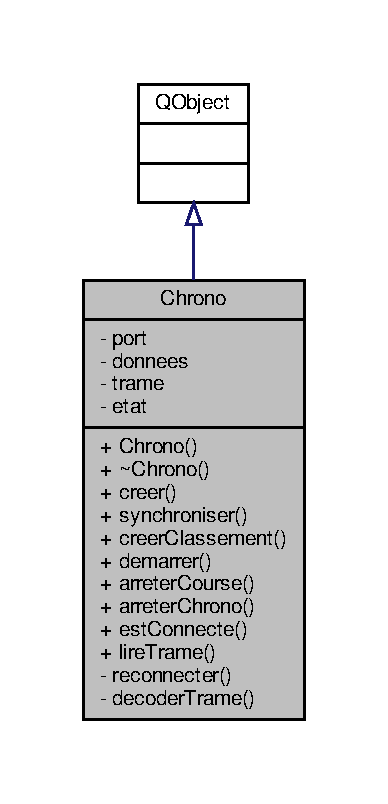
\includegraphics[width=186pt]{class_chrono__coll__graph}
\end{center}
\end{figure}
\subsubsection*{Connecteurs publics}
\begin{DoxyCompactItemize}
\item 
void \hyperlink{class_chrono_ae7c3c8494ace02f4c9dd714f6f0e574a}{lire\+Trame} ()
\begin{DoxyCompactList}\small\item\em Méthode \hyperlink{class_chrono_ae7c3c8494ace02f4c9dd714f6f0e574a}{lire\+Trame()} de la classe \hyperlink{class_chrono}{Chrono}. \end{DoxyCompactList}\end{DoxyCompactItemize}
\subsubsection*{Signaux}
\begin{DoxyCompactItemize}
\item 
void \hyperlink{class_chrono_a60ef5586dd429ab616c2b02c143daedf}{chrono\+Creer} ()
\item 
void \hyperlink{class_chrono_a4ae8a6eb8da3f43eb15392b08f391237}{chrono\+Synchroniser} ()
\item 
void \hyperlink{class_chrono_aea06e35eac092428e821a07a5e2df64c}{classement\+Cree} ()
\item 
void \hyperlink{class_chrono_a590290b81a290717bfe1b87f1c605181}{chrono\+Lance} ()
\item 
void \hyperlink{class_chrono_a054799dc10e42daff8545689a61aea35}{course\+Arretee} ()
\item 
void \hyperlink{class_chrono_a5e28dfd0010e34a19ccb03b9dcbe4dcd}{chrono\+Arrete} ()
\item 
void \hyperlink{class_chrono_ab697687f26503bee2b9c9e6f2a073f14}{chrono\+Recommence} ()
\item 
void \hyperlink{class_chrono_a38cf60f7ab1969d7fd1e672868156135}{nouvelle\+Arrivee} (Q\+String temps\+Arrivee)
\end{DoxyCompactItemize}
\subsubsection*{Fonctions membres publiques}
\begin{DoxyCompactItemize}
\item 
\hyperlink{class_chrono_a01eb40847915c49c48c7dc9ca63cbd99}{Chrono} (\hyperlink{class_q_object}{Q\+Object} $\ast$parent=nullptr)
\begin{DoxyCompactList}\small\item\em Constructeur de la classe \hyperlink{class_chrono}{Chrono}. \end{DoxyCompactList}\item 
\hyperlink{class_chrono_aaba59dd29fe5d3469c147cd2b014adc1}{$\sim$\+Chrono} ()
\begin{DoxyCompactList}\small\item\em Destructeur de la fenêtre principale. \end{DoxyCompactList}\item 
void \hyperlink{class_chrono_a74d85a4e856e2e59afacaa061feb7b75}{creer} ()
\begin{DoxyCompactList}\small\item\em Méthode \hyperlink{class_chrono_a74d85a4e856e2e59afacaa061feb7b75}{creer()} de la classe \hyperlink{class_chrono}{Chrono}. \end{DoxyCompactList}\item 
bool \hyperlink{class_chrono_a858a209a6d366b3adb95bcf593645d6a}{synchroniser} ()
\begin{DoxyCompactList}\small\item\em Méthode \hyperlink{class_chrono_a858a209a6d366b3adb95bcf593645d6a}{synchroniser()} de la classe \hyperlink{class_chrono}{Chrono}. \end{DoxyCompactList}\item 
bool \hyperlink{class_chrono_a0d7e3e50fcef0f2b0b7bfadc3d4f737d}{creer\+Classement} ()
\begin{DoxyCompactList}\small\item\em Méthode \hyperlink{class_chrono_a0d7e3e50fcef0f2b0b7bfadc3d4f737d}{creer\+Classement()} de la classe \hyperlink{class_chrono}{Chrono}. \end{DoxyCompactList}\item 
bool \hyperlink{class_chrono_a2ee875c24eb14f09011a40dfb3f1921f}{demarrer} ()
\begin{DoxyCompactList}\small\item\em Méthode \hyperlink{class_chrono_a2ee875c24eb14f09011a40dfb3f1921f}{demarrer()} de la classe \hyperlink{class_chrono}{Chrono}. \end{DoxyCompactList}\item 
bool \hyperlink{class_chrono_a2a0d899b09eb044caa83b41574ac5edf}{arreter\+Course} ()
\begin{DoxyCompactList}\small\item\em Méthode \hyperlink{class_chrono_a2a0d899b09eb044caa83b41574ac5edf}{arreter\+Course()} de la classe \hyperlink{class_chrono}{Chrono}. \end{DoxyCompactList}\item 
bool \hyperlink{class_chrono_a5e2781ab78dcaa0ecb37e301399d819b}{arreter\+Chrono} ()
\begin{DoxyCompactList}\small\item\em Méthode \hyperlink{class_chrono_a5e2781ab78dcaa0ecb37e301399d819b}{arreter\+Chrono()} de la classe \hyperlink{class_chrono}{Chrono}. \end{DoxyCompactList}\item 
bool \hyperlink{class_chrono_aaad6d9079f2de1c09092f97614009f62}{est\+Connecte} ()
\begin{DoxyCompactList}\small\item\em Méthode \hyperlink{class_chrono_aaad6d9079f2de1c09092f97614009f62}{est\+Connecte()} de la classe \hyperlink{class_chrono}{Chrono}. \end{DoxyCompactList}\end{DoxyCompactItemize}
\subsubsection*{Fonctions membres privées}
\begin{DoxyCompactItemize}
\item 
bool \hyperlink{class_chrono_a80305a5dae33e8cd99604e809589564b}{reconnecter} ()
\begin{DoxyCompactList}\small\item\em Méthode \hyperlink{class_chrono_a80305a5dae33e8cd99604e809589564b}{reconnecter()} de la classe \hyperlink{class_chrono}{Chrono}. \end{DoxyCompactList}\item 
void \hyperlink{class_chrono_a9a66b4e81385e2c354805548b94cdfb6}{decoder\+Trame} ()
\begin{DoxyCompactList}\small\item\em Méthode \hyperlink{class_chrono_a9a66b4e81385e2c354805548b94cdfb6}{decoder\+Trame()} de la classe \hyperlink{class_chrono}{Chrono}. \end{DoxyCompactList}\end{DoxyCompactItemize}
\subsubsection*{Attributs privés}
\begin{DoxyCompactItemize}
\item 
Q\+Serial\+Port $\ast$ \hyperlink{class_chrono_aca5fbe0eebd7f876f954d4a99c564167}{port}
\begin{DoxyCompactList}\small\item\em Port R\+S232 du T\+AG H\+E\+U\+ER. \end{DoxyCompactList}\item 
Q\+Byte\+Array \hyperlink{class_chrono_a7771ee85460ad5f61f96cea2267ae23f}{donnees}
\begin{DoxyCompactList}\small\item\em Données brutes d\textquotesingle{}une trame T\+H\+C\+O\+M08. \end{DoxyCompactList}\item 
Q\+String \hyperlink{class_chrono_a26f2155aa6e5ef4296e5456b64a713b5}{trame}
\begin{DoxyCompactList}\small\item\em Trame T\+H\+C\+O\+M08. \end{DoxyCompactList}\item 
unsigned int \hyperlink{class_chrono_ad82d4f2a230290aa9695f12bf5ac02e8}{etat}
\begin{DoxyCompactList}\small\item\em État du chronomètre. \end{DoxyCompactList}\end{DoxyCompactItemize}


\subsubsection{Description détaillée}
Déclaration de la classe \hyperlink{class_chrono}{Chrono}. 

\begin{DoxyAuthor}{Auteur}
Michael Andréo
\end{DoxyAuthor}
\begin{DoxyVersion}{Version}
1.\+1 
\end{DoxyVersion}


\subsubsection{Documentation des constructeurs et destructeur}
\mbox{\Hypertarget{class_chrono_a01eb40847915c49c48c7dc9ca63cbd99}\label{class_chrono_a01eb40847915c49c48c7dc9ca63cbd99}} 
\index{Chrono@{Chrono}!Chrono@{Chrono}}
\index{Chrono@{Chrono}!Chrono@{Chrono}}
\paragraph{\texorpdfstring{Chrono()}{Chrono()}}
{\footnotesize\ttfamily Chrono\+::\+Chrono (\begin{DoxyParamCaption}\item[{\hyperlink{class_q_object}{Q\+Object} $\ast$}]{parent = {\ttfamily nullptr} }\end{DoxyParamCaption})}



Constructeur de la classe \hyperlink{class_chrono}{Chrono}. 


\begin{DoxyParams}{Paramètres}
{\em parent} & \hyperlink{class_q_object}{Q\+Object} Adresse de l\textquotesingle{}objet Qt parent (0 = pas de parent car c\textquotesingle{}est la fenêtre principale) \\
\hline
\end{DoxyParams}


Références \hyperlink{class_chrono_ad82d4f2a230290aa9695f12bf5ac02e8}{etat}, \hyperlink{chrono_8h_a614217d263be1fb1a5f76e2ff7be19a2}{P\+O\+RT}, et \hyperlink{class_chrono_aca5fbe0eebd7f876f954d4a99c564167}{port}.


\begin{DoxyCode}
00020                               : \hyperlink{class_q_object}{QObject} (parent)
00021 \{
00022     \hyperlink{class_chrono_aca5fbe0eebd7f876f954d4a99c564167}{port} = \textcolor{keyword}{new} QSerialPort(\hyperlink{chrono_8h_a614217d263be1fb1a5f76e2ff7be19a2}{PORT});
00023     \hyperlink{class_chrono_aca5fbe0eebd7f876f954d4a99c564167}{port}->setBaudRate(QSerialPort::Baud9600);
00024     \hyperlink{class_chrono_aca5fbe0eebd7f876f954d4a99c564167}{port}->setFlowControl(QSerialPort::NoFlowControl);
00025     \hyperlink{class_chrono_aca5fbe0eebd7f876f954d4a99c564167}{port}->setParity(QSerialPort::NoParity);
00026     \hyperlink{class_chrono_aca5fbe0eebd7f876f954d4a99c564167}{port}->setDataBits(QSerialPort::Data8);
00027     \hyperlink{class_chrono_aca5fbe0eebd7f876f954d4a99c564167}{port}->setStopBits(QSerialPort::OneStop);
00028     \hyperlink{class_chrono_aca5fbe0eebd7f876f954d4a99c564167}{port}->open(QIODevice::ReadWrite);
00029 
00030     \hyperlink{class_chrono_ad82d4f2a230290aa9695f12bf5ac02e8}{etat} = 0;
00031 
00032     qDebug() << Q\_FUNC\_INFO << \textcolor{stringliteral}{"Etat port : "} << \hyperlink{class_chrono_aca5fbe0eebd7f876f954d4a99c564167}{port}->isOpen();
00033 \}
\end{DoxyCode}
\mbox{\Hypertarget{class_chrono_aaba59dd29fe5d3469c147cd2b014adc1}\label{class_chrono_aaba59dd29fe5d3469c147cd2b014adc1}} 
\index{Chrono@{Chrono}!````~Chrono@{$\sim$\+Chrono}}
\index{````~Chrono@{$\sim$\+Chrono}!Chrono@{Chrono}}
\paragraph{\texorpdfstring{$\sim$\+Chrono()}{~Chrono()}}
{\footnotesize\ttfamily Chrono\+::$\sim$\+Chrono (\begin{DoxyParamCaption}{ }\end{DoxyParamCaption})}



Destructeur de la fenêtre principale. 



Références \hyperlink{class_chrono_aca5fbe0eebd7f876f954d4a99c564167}{port}.


\begin{DoxyCode}
00040 \{
00041     \hyperlink{class_chrono_aca5fbe0eebd7f876f954d4a99c564167}{port}->close();
00042 \}
\end{DoxyCode}


\subsubsection{Documentation des fonctions membres}
\mbox{\Hypertarget{class_chrono_a5e2781ab78dcaa0ecb37e301399d819b}\label{class_chrono_a5e2781ab78dcaa0ecb37e301399d819b}} 
\index{Chrono@{Chrono}!arreter\+Chrono@{arreter\+Chrono}}
\index{arreter\+Chrono@{arreter\+Chrono}!Chrono@{Chrono}}
\paragraph{\texorpdfstring{arreter\+Chrono()}{arreterChrono()}}
{\footnotesize\ttfamily bool Chrono\+::arreter\+Chrono (\begin{DoxyParamCaption}{ }\end{DoxyParamCaption})}



Méthode \hyperlink{class_chrono_a5e2781ab78dcaa0ecb37e301399d819b}{arreter\+Chrono()} de la classe \hyperlink{class_chrono}{Chrono}. 

Si le port est ouvert on écrit la trame M\+O\+D\+E\+ND \begin{DoxyReturn}{Renvoie}
bool 
\end{DoxyReturn}


Références \hyperlink{chrono_8h_a95708e00882b95a7b2d68b2f75c3913c}{M\+O\+D\+E\+ND}, \hyperlink{class_chrono_aca5fbe0eebd7f876f954d4a99c564167}{port}, et \hyperlink{class_chrono_a26f2155aa6e5ef4296e5456b64a713b5}{trame}.



Référencé par \hyperlink{class_course_a939635ac8301a7018475cc2ce347375f}{Course\+::arreter\+Chrono()}.


\begin{DoxyCode}
00282 \{
00283     \textcolor{keywordflow}{if}(!\hyperlink{class_chrono_aca5fbe0eebd7f876f954d4a99c564167}{port}->isOpen())
00284         \textcolor{keywordflow}{return} \textcolor{keyword}{false};
00285     qDebug() << Q\_FUNC\_INFO << \textcolor{stringliteral}{"MODEND"};
00286     \hyperlink{class_chrono_a26f2155aa6e5ef4296e5456b64a713b5}{trame} = \hyperlink{chrono_8h_a95708e00882b95a7b2d68b2f75c3913c}{MODEND};
00287     qDebug() << Q\_FUNC\_INFO << \textcolor{stringliteral}{"trame"} << \hyperlink{class_chrono_a26f2155aa6e5ef4296e5456b64a713b5}{trame};
00288     \textcolor{keywordtype}{int} nb = int(\hyperlink{class_chrono_aca5fbe0eebd7f876f954d4a99c564167}{port}->write(trame.toLatin1()));
00289     \textcolor{keywordflow}{if}(nb > 0)
00290         \textcolor{keywordflow}{return} \textcolor{keyword}{true};
00291     \textcolor{keywordflow}{else}
00292         \textcolor{keywordflow}{return} \textcolor{keyword}{false};
00293 \}
\end{DoxyCode}
\mbox{\Hypertarget{class_chrono_a2a0d899b09eb044caa83b41574ac5edf}\label{class_chrono_a2a0d899b09eb044caa83b41574ac5edf}} 
\index{Chrono@{Chrono}!arreter\+Course@{arreter\+Course}}
\index{arreter\+Course@{arreter\+Course}!Chrono@{Chrono}}
\paragraph{\texorpdfstring{arreter\+Course()}{arreterCourse()}}
{\footnotesize\ttfamily bool Chrono\+::arreter\+Course (\begin{DoxyParamCaption}{ }\end{DoxyParamCaption})}



Méthode \hyperlink{class_chrono_a2a0d899b09eb044caa83b41574ac5edf}{arreter\+Course()} de la classe \hyperlink{class_chrono}{Chrono}. 

Si le port est ouvert on écrit la trame C\+L\+O\+S\+E\+R\+UN 

Références \hyperlink{chrono_8h_aadc6271993e3725db8c6640289f8d2bb}{C\+L\+O\+S\+E\+R\+UN}, \hyperlink{class_chrono_aca5fbe0eebd7f876f954d4a99c564167}{port}, et \hyperlink{class_chrono_a26f2155aa6e5ef4296e5456b64a713b5}{trame}.



Référencé par \hyperlink{class_course_a4426310a411d8ecf7f4a2dc64c24a42d}{Course\+::arreter\+Classement()}.


\begin{DoxyCode}
00262 \{
00263     \textcolor{keywordflow}{if}(!\hyperlink{class_chrono_aca5fbe0eebd7f876f954d4a99c564167}{port}->isOpen())
00264         \textcolor{keywordflow}{return} \textcolor{keyword}{false};
00265     qDebug() << Q\_FUNC\_INFO << \textcolor{stringliteral}{"CLOSERUN"};
00266     \hyperlink{class_chrono_a26f2155aa6e5ef4296e5456b64a713b5}{trame} = \hyperlink{chrono_8h_aadc6271993e3725db8c6640289f8d2bb}{CLOSERUN};
00267     qDebug() << Q\_FUNC\_INFO << \textcolor{stringliteral}{"trame"} << \hyperlink{class_chrono_a26f2155aa6e5ef4296e5456b64a713b5}{trame};
00268     \textcolor{keywordtype}{int} nb = int(\hyperlink{class_chrono_aca5fbe0eebd7f876f954d4a99c564167}{port}->write(trame.toLatin1()));
00269     \textcolor{keywordflow}{if}(nb > 0)
00270         \textcolor{keywordflow}{return} \textcolor{keyword}{true};
00271     \textcolor{keywordflow}{else}
00272         \textcolor{keywordflow}{return} \textcolor{keyword}{false};
00273 \}
\end{DoxyCode}
\mbox{\Hypertarget{class_chrono_a5e28dfd0010e34a19ccb03b9dcbe4dcd}\label{class_chrono_a5e28dfd0010e34a19ccb03b9dcbe4dcd}} 
\index{Chrono@{Chrono}!chrono\+Arrete@{chrono\+Arrete}}
\index{chrono\+Arrete@{chrono\+Arrete}!Chrono@{Chrono}}
\paragraph{\texorpdfstring{chrono\+Arrete}{chronoArrete}}
{\footnotesize\ttfamily void Chrono\+::chrono\+Arrete (\begin{DoxyParamCaption}{ }\end{DoxyParamCaption})\hspace{0.3cm}{\ttfamily [signal]}}



Référencé par \hyperlink{class_chrono_a9a66b4e81385e2c354805548b94cdfb6}{decoder\+Trame()}.

\mbox{\Hypertarget{class_chrono_a60ef5586dd429ab616c2b02c143daedf}\label{class_chrono_a60ef5586dd429ab616c2b02c143daedf}} 
\index{Chrono@{Chrono}!chrono\+Creer@{chrono\+Creer}}
\index{chrono\+Creer@{chrono\+Creer}!Chrono@{Chrono}}
\paragraph{\texorpdfstring{chrono\+Creer}{chronoCreer}}
{\footnotesize\ttfamily void Chrono\+::chrono\+Creer (\begin{DoxyParamCaption}{ }\end{DoxyParamCaption})\hspace{0.3cm}{\ttfamily [signal]}}



Référencé par \hyperlink{class_chrono_a9a66b4e81385e2c354805548b94cdfb6}{decoder\+Trame()}.

\mbox{\Hypertarget{class_chrono_a590290b81a290717bfe1b87f1c605181}\label{class_chrono_a590290b81a290717bfe1b87f1c605181}} 
\index{Chrono@{Chrono}!chrono\+Lance@{chrono\+Lance}}
\index{chrono\+Lance@{chrono\+Lance}!Chrono@{Chrono}}
\paragraph{\texorpdfstring{chrono\+Lance}{chronoLance}}
{\footnotesize\ttfamily void Chrono\+::chrono\+Lance (\begin{DoxyParamCaption}{ }\end{DoxyParamCaption})\hspace{0.3cm}{\ttfamily [signal]}}



Référencé par \hyperlink{class_chrono_a9a66b4e81385e2c354805548b94cdfb6}{decoder\+Trame()}.

\mbox{\Hypertarget{class_chrono_ab697687f26503bee2b9c9e6f2a073f14}\label{class_chrono_ab697687f26503bee2b9c9e6f2a073f14}} 
\index{Chrono@{Chrono}!chrono\+Recommence@{chrono\+Recommence}}
\index{chrono\+Recommence@{chrono\+Recommence}!Chrono@{Chrono}}
\paragraph{\texorpdfstring{chrono\+Recommence}{chronoRecommence}}
{\footnotesize\ttfamily void Chrono\+::chrono\+Recommence (\begin{DoxyParamCaption}{ }\end{DoxyParamCaption})\hspace{0.3cm}{\ttfamily [signal]}}



Référencé par \hyperlink{class_chrono_a9a66b4e81385e2c354805548b94cdfb6}{decoder\+Trame()}.

\mbox{\Hypertarget{class_chrono_a4ae8a6eb8da3f43eb15392b08f391237}\label{class_chrono_a4ae8a6eb8da3f43eb15392b08f391237}} 
\index{Chrono@{Chrono}!chrono\+Synchroniser@{chrono\+Synchroniser}}
\index{chrono\+Synchroniser@{chrono\+Synchroniser}!Chrono@{Chrono}}
\paragraph{\texorpdfstring{chrono\+Synchroniser}{chronoSynchroniser}}
{\footnotesize\ttfamily void Chrono\+::chrono\+Synchroniser (\begin{DoxyParamCaption}{ }\end{DoxyParamCaption})\hspace{0.3cm}{\ttfamily [signal]}}



Référencé par \hyperlink{class_chrono_a9a66b4e81385e2c354805548b94cdfb6}{decoder\+Trame()}.

\mbox{\Hypertarget{class_chrono_aea06e35eac092428e821a07a5e2df64c}\label{class_chrono_aea06e35eac092428e821a07a5e2df64c}} 
\index{Chrono@{Chrono}!classement\+Cree@{classement\+Cree}}
\index{classement\+Cree@{classement\+Cree}!Chrono@{Chrono}}
\paragraph{\texorpdfstring{classement\+Cree}{classementCree}}
{\footnotesize\ttfamily void Chrono\+::classement\+Cree (\begin{DoxyParamCaption}{ }\end{DoxyParamCaption})\hspace{0.3cm}{\ttfamily [signal]}}



Référencé par \hyperlink{class_chrono_a9a66b4e81385e2c354805548b94cdfb6}{decoder\+Trame()}.

\mbox{\Hypertarget{class_chrono_a054799dc10e42daff8545689a61aea35}\label{class_chrono_a054799dc10e42daff8545689a61aea35}} 
\index{Chrono@{Chrono}!course\+Arretee@{course\+Arretee}}
\index{course\+Arretee@{course\+Arretee}!Chrono@{Chrono}}
\paragraph{\texorpdfstring{course\+Arretee}{courseArretee}}
{\footnotesize\ttfamily void Chrono\+::course\+Arretee (\begin{DoxyParamCaption}{ }\end{DoxyParamCaption})\hspace{0.3cm}{\ttfamily [signal]}}



Référencé par \hyperlink{class_chrono_a9a66b4e81385e2c354805548b94cdfb6}{decoder\+Trame()}.

\mbox{\Hypertarget{class_chrono_a74d85a4e856e2e59afacaa061feb7b75}\label{class_chrono_a74d85a4e856e2e59afacaa061feb7b75}} 
\index{Chrono@{Chrono}!creer@{creer}}
\index{creer@{creer}!Chrono@{Chrono}}
\paragraph{\texorpdfstring{creer()}{creer()}}
{\footnotesize\ttfamily void Chrono\+::creer (\begin{DoxyParamCaption}{ }\end{DoxyParamCaption})}



Méthode \hyperlink{class_chrono_a74d85a4e856e2e59afacaa061feb7b75}{creer()} de la classe \hyperlink{class_chrono}{Chrono}. 

Si le port est ouvert on écrit la trame M\+O\+D\+E\+C\+L\+O\+CK 

Références \hyperlink{class_chrono_ae7c3c8494ace02f4c9dd714f6f0e574a}{lire\+Trame()}, \hyperlink{chrono_8h_a51714542fe5fc5c442f126a96c568050}{M\+O\+D\+E\+C\+L\+O\+CK}, \hyperlink{class_chrono_aca5fbe0eebd7f876f954d4a99c564167}{port}, et \hyperlink{class_chrono_a26f2155aa6e5ef4296e5456b64a713b5}{trame}.



Référencé par \hyperlink{class_course_a6eb96222d8dc1f352e28f36e9b414448}{Course\+::creer\+Chrono()}, et \hyperlink{class_chrono_a80305a5dae33e8cd99604e809589564b}{reconnecter()}.


\begin{DoxyCode}
00189 \{
00190     \textcolor{keywordflow}{if}(\hyperlink{class_chrono_aca5fbe0eebd7f876f954d4a99c564167}{port}->isOpen())
00191     \{
00192         connect(\hyperlink{class_chrono_aca5fbe0eebd7f876f954d4a99c564167}{port}, SIGNAL(readyRead()), \textcolor{keyword}{this}, SLOT(\hyperlink{class_chrono_ae7c3c8494ace02f4c9dd714f6f0e574a}{lireTrame}()));
00193         qDebug() << Q\_FUNC\_INFO << \textcolor{stringliteral}{"MODECLOCK"};
00194         \hyperlink{class_chrono_a26f2155aa6e5ef4296e5456b64a713b5}{trame} = \hyperlink{chrono_8h_a51714542fe5fc5c442f126a96c568050}{MODECLOCK};
00195         qDebug() << Q\_FUNC\_INFO << \textcolor{stringliteral}{"trame émise"} << \hyperlink{class_chrono_a26f2155aa6e5ef4296e5456b64a713b5}{trame};
00196         \hyperlink{class_chrono_aca5fbe0eebd7f876f954d4a99c564167}{port}->write(trame.toLatin1());
00197     \}
00198 \}
\end{DoxyCode}
\mbox{\Hypertarget{class_chrono_a0d7e3e50fcef0f2b0b7bfadc3d4f737d}\label{class_chrono_a0d7e3e50fcef0f2b0b7bfadc3d4f737d}} 
\index{Chrono@{Chrono}!creer\+Classement@{creer\+Classement}}
\index{creer\+Classement@{creer\+Classement}!Chrono@{Chrono}}
\paragraph{\texorpdfstring{creer\+Classement()}{creerClassement()}}
{\footnotesize\ttfamily bool Chrono\+::creer\+Classement (\begin{DoxyParamCaption}{ }\end{DoxyParamCaption})}



Méthode \hyperlink{class_chrono_a0d7e3e50fcef0f2b0b7bfadc3d4f737d}{creer\+Classement()} de la classe \hyperlink{class_chrono}{Chrono}. 

Si le port est ouvert on écrit la trame N\+E\+W\+R\+UN 

Références \hyperlink{chrono_8h_a4dcfb7100df159ff3082add0247cd3ee}{N\+E\+W\+R\+UN}, \hyperlink{class_chrono_aca5fbe0eebd7f876f954d4a99c564167}{port}, et \hyperlink{class_chrono_a26f2155aa6e5ef4296e5456b64a713b5}{trame}.



Référencé par \hyperlink{class_course_a90c66d620f0726d92c40069f052e0cd0}{Course\+::a\+Chrono\+Synchronise()}.


\begin{DoxyCode}
00225 \{
00226     \textcolor{keywordflow}{if}(!\hyperlink{class_chrono_aca5fbe0eebd7f876f954d4a99c564167}{port}->isOpen())
00227         \textcolor{keywordflow}{return} \textcolor{keyword}{false};
00228     qDebug() << Q\_FUNC\_INFO << \textcolor{stringliteral}{"NEWRUN"};
00229     \hyperlink{class_chrono_a26f2155aa6e5ef4296e5456b64a713b5}{trame} = \hyperlink{chrono_8h_a4dcfb7100df159ff3082add0247cd3ee}{NEWRUN};
00230     \textcolor{keywordtype}{int} nb = int(\hyperlink{class_chrono_aca5fbe0eebd7f876f954d4a99c564167}{port}->write(\hyperlink{class_chrono_a26f2155aa6e5ef4296e5456b64a713b5}{trame}.toLatin1()));
00231     \textcolor{keywordflow}{if}(nb > 0)
00232         \textcolor{keywordflow}{return} \textcolor{keyword}{true};
00233     \textcolor{keywordflow}{else}
00234         \textcolor{keywordflow}{return} \textcolor{keyword}{false};
00235 \}
\end{DoxyCode}
\mbox{\Hypertarget{class_chrono_a9a66b4e81385e2c354805548b94cdfb6}\label{class_chrono_a9a66b4e81385e2c354805548b94cdfb6}} 
\index{Chrono@{Chrono}!decoder\+Trame@{decoder\+Trame}}
\index{decoder\+Trame@{decoder\+Trame}!Chrono@{Chrono}}
\paragraph{\texorpdfstring{decoder\+Trame()}{decoderTrame()}}
{\footnotesize\ttfamily void Chrono\+::decoder\+Trame (\begin{DoxyParamCaption}{ }\end{DoxyParamCaption})\hspace{0.3cm}{\ttfamily [private]}}



Méthode \hyperlink{class_chrono_a9a66b4e81385e2c354805548b94cdfb6}{decoder\+Trame()} de la classe \hyperlink{class_chrono}{Chrono}. 

Décode les trames émise du T\+AG H\+E\+U\+ER 

Références \hyperlink{chrono_8h_ad727a8a4b248052dfc12e6b4320d5f29}{C\+H\+A\+M\+P\+S\+\_\+\+T\+R\+A\+M\+E\+\_\+\+T\+E\+M\+PS}, \hyperlink{class_chrono_a5e28dfd0010e34a19ccb03b9dcbe4dcd}{chrono\+Arrete()}, \hyperlink{class_chrono_a60ef5586dd429ab616c2b02c143daedf}{chrono\+Creer()}, \hyperlink{class_chrono_a590290b81a290717bfe1b87f1c605181}{chrono\+Lance()}, \hyperlink{class_chrono_ab697687f26503bee2b9c9e6f2a073f14}{chrono\+Recommence()}, \hyperlink{class_chrono_a4ae8a6eb8da3f43eb15392b08f391237}{chrono\+Synchroniser()}, \hyperlink{class_chrono_aea06e35eac092428e821a07a5e2df64c}{classement\+Cree()}, \hyperlink{class_chrono_a054799dc10e42daff8545689a61aea35}{course\+Arretee()}, \hyperlink{class_chrono_ad82d4f2a230290aa9695f12bf5ac02e8}{etat}, \hyperlink{chrono_8h_aedfd738fe89f9d5e1a9d2c8a08786815}{E\+T\+A\+T\+\_\+\+C\+L\+O\+S\+E\+R\+UN}, \hyperlink{chrono_8h_ac7f40e9c99ad9f32b52bbe642c29fa35}{E\+T\+A\+T\+\_\+\+M\+O\+D\+E\+C\+L\+O\+CK}, \hyperlink{chrono_8h_a8d3c4247ab94fd8e6757811fb4001f1e}{E\+T\+A\+T\+\_\+\+M\+O\+D\+E\+ND}, \hyperlink{chrono_8h_a3870f0e4dd2af74ba5c110e419d65d99}{E\+T\+A\+T\+\_\+\+N\+E\+W\+R\+UN}, \hyperlink{chrono_8h_ab4e7883be172f7dac0123a67e9c6c655}{E\+T\+A\+T\+\_\+\+N\+E\+W\+S\+Y\+N\+C\+H\+RO}, \hyperlink{chrono_8h_af1a61de8ee28781dbc28e0d7d43c158e}{E\+T\+A\+T\+\_\+\+N\+O\+N\+S\+Y\+N\+C\+H\+RO}, \hyperlink{chrono_8h_ab6827e7b3f5ba7079e57df316b490544}{E\+T\+A\+T\+\_\+\+S\+T\+A\+R\+T\+M\+A\+N\+U\+A\+L\+S\+Y\+N\+C\+H\+RO}, \hyperlink{class_chrono_a38cf60f7ab1969d7fd1e672868156135}{nouvelle\+Arrivee()}, \hyperlink{class_chrono_a80305a5dae33e8cd99604e809589564b}{reconnecter()}, \hyperlink{class_chrono_a26f2155aa6e5ef4296e5456b64a713b5}{trame}, \hyperlink{chrono_8h_a2c9f7b58ba826bd8365c9a611389fe42}{T\+R\+A\+M\+E\+\_\+\+A\+C\+Q\+U\+I\+T\+T\+E\+M\+E\+NT}, \hyperlink{chrono_8h_a24bef153968288b19cfda35989658fe1}{T\+R\+A\+M\+E\+\_\+\+C\+O\+U\+R\+S\+E\+\_\+\+T\+E\+R\+M\+I\+N\+EE}, et \hyperlink{chrono_8h_af6d8d017aa1c07e0c9900e13a60959ba}{T\+R\+A\+M\+E\+\_\+\+T\+E\+M\+PS}.



Référencé par \hyperlink{class_chrono_ae7c3c8494ace02f4c9dd714f6f0e574a}{lire\+Trame()}.


\begin{DoxyCode}
00072 \{
00073     \textcolor{comment}{/*}
00074 \textcolor{comment}{      Liste des trames reçues :}
00075 \textcolor{comment}{      - "AK X" acquittement avec : X = 'C' accepted, 'F' rejected, 'R' not supported}
00076 \textcolor{comment}{      - "TS 00:00:00 00/00/01" synchro}
00077 \textcolor{comment}{      - "&P 003 XX 90 00:00:00 0" paramètre 003 (demande du numéro de course) XX = le numéro de course}
00078 \textcolor{comment}{      - "TN 1 2     3.71300  365" temps}
00079 \textcolor{comment}{      - "CL XX" close course XX = le numéro de course terminée}
00080 \textcolor{comment}{     */}
00081 
00082     \hyperlink{class_chrono_a26f2155aa6e5ef4296e5456b64a713b5}{trame}.remove(\textcolor{stringliteral}{"\(\backslash\)r\(\backslash\)n"});
00083     qDebug() << Q\_FUNC\_INFO << \textcolor{stringliteral}{"Trame after remove rn:\(\backslash\)t"} << \hyperlink{class_chrono_a26f2155aa6e5ef4296e5456b64a713b5}{trame};
00084 
00085     QStringList champsTrame;
00086     \textcolor{keywordflow}{if}(trame.startsWith(\hyperlink{chrono_8h_a2c9f7b58ba826bd8365c9a611389fe42}{TRAME\_ACQUITTEMENT}))
00087     \{
00088         champsTrame = trame.split(\textcolor{stringliteral}{" "}, QString::SkipEmptyParts);
00089         qDebug() << Q\_FUNC\_INFO << \textcolor{stringliteral}{"Trame acquitement :"} << champsTrame[1];
00090 
00091         \textcolor{keywordflow}{if}(champsTrame[1].startsWith(\textcolor{stringliteral}{"C"}))
00092         \{
00093             \textcolor{keywordflow}{if}(\hyperlink{class_chrono_ad82d4f2a230290aa9695f12bf5ac02e8}{etat} == \hyperlink{chrono_8h_a8d3c4247ab94fd8e6757811fb4001f1e}{ETAT\_MODEND})
00094             \{
00095                 \hyperlink{class_chrono_ad82d4f2a230290aa9695f12bf5ac02e8}{etat} = \hyperlink{chrono_8h_af1a61de8ee28781dbc28e0d7d43c158e}{ETAT\_NONSYNCHRO};
00096                 emit \hyperlink{class_chrono_ab697687f26503bee2b9c9e6f2a073f14}{chronoRecommence}();
00097             \}
00098             \textcolor{comment}{//première trame d'acquittement}
00099             \textcolor{keywordflow}{if}(\hyperlink{class_chrono_ad82d4f2a230290aa9695f12bf5ac02e8}{etat} == \hyperlink{chrono_8h_af1a61de8ee28781dbc28e0d7d43c158e}{ETAT\_NONSYNCHRO})
00100             \{
00101                 \hyperlink{class_chrono_ad82d4f2a230290aa9695f12bf5ac02e8}{etat} = \hyperlink{chrono_8h_ac7f40e9c99ad9f32b52bbe642c29fa35}{ETAT\_MODECLOCK};
00102                 emit \hyperlink{class_chrono_a60ef5586dd429ab616c2b02c143daedf}{chronoCreer}();
00103                 qDebug() << Q\_FUNC\_INFO << \textcolor{stringliteral}{"AK\(\backslash\)tETAT chrono creer! 1"} << \hyperlink{class_chrono_ad82d4f2a230290aa9695f12bf5ac02e8}{etat};
00104             \}
00105             \textcolor{comment}{//deuxieme trame d'acquittement}
00106             \textcolor{keywordflow}{else} \textcolor{keywordflow}{if}(\hyperlink{class_chrono_ad82d4f2a230290aa9695f12bf5ac02e8}{etat} == \hyperlink{chrono_8h_ac7f40e9c99ad9f32b52bbe642c29fa35}{ETAT\_MODECLOCK})
00107             \{
00108                 \hyperlink{class_chrono_ad82d4f2a230290aa9695f12bf5ac02e8}{etat} = \hyperlink{chrono_8h_ab4e7883be172f7dac0123a67e9c6c655}{ETAT\_NEWSYNCHRO};
00109                 emit \hyperlink{class_chrono_a4ae8a6eb8da3f43eb15392b08f391237}{chronoSynchroniser}();
00110                 qDebug() << Q\_FUNC\_INFO << \textcolor{stringliteral}{"AK\(\backslash\)tETAT Mode clock 2"} << \hyperlink{class_chrono_ad82d4f2a230290aa9695f12bf5ac02e8}{etat};
00111             \}
00112             \textcolor{comment}{//troisieme trame d'acquittement}
00113             \textcolor{keywordflow}{else} \textcolor{keywordflow}{if}(\hyperlink{class_chrono_ad82d4f2a230290aa9695f12bf5ac02e8}{etat} == \hyperlink{chrono_8h_ab4e7883be172f7dac0123a67e9c6c655}{ETAT\_NEWSYNCHRO})
00114             \{
00115                 \hyperlink{class_chrono_ad82d4f2a230290aa9695f12bf5ac02e8}{etat} = \hyperlink{chrono_8h_a3870f0e4dd2af74ba5c110e419d65d99}{ETAT\_NEWRUN};
00116                 emit \hyperlink{class_chrono_aea06e35eac092428e821a07a5e2df64c}{classementCree}();
00117                 qDebug() << Q\_FUNC\_INFO << \textcolor{stringliteral}{"ETAT NEW SYNCHR 3"} << \hyperlink{class_chrono_ad82d4f2a230290aa9695f12bf5ac02e8}{etat};
00118             \}
00119             \textcolor{comment}{//quatrième trame d'acquittement}
00120             \textcolor{keywordflow}{else} \textcolor{keywordflow}{if}(\hyperlink{class_chrono_ad82d4f2a230290aa9695f12bf5ac02e8}{etat} == \hyperlink{chrono_8h_a3870f0e4dd2af74ba5c110e419d65d99}{ETAT\_NEWRUN})
00121             \{
00122                 \hyperlink{class_chrono_ad82d4f2a230290aa9695f12bf5ac02e8}{etat} = \hyperlink{chrono_8h_ab6827e7b3f5ba7079e57df316b490544}{ETAT\_STARTMANUALSYNCHRO};
00123                 emit \hyperlink{class_chrono_a590290b81a290717bfe1b87f1c605181}{chronoLance}();
00124                 qDebug() << Q\_FUNC\_INFO << \textcolor{stringliteral}{"ETAT NEWRUN 4"} << \hyperlink{class_chrono_ad82d4f2a230290aa9695f12bf5ac02e8}{etat};
00125             \}
00126             \textcolor{comment}{//cinquième trame d'acquittement}
00127             \textcolor{keywordflow}{else} \textcolor{keywordflow}{if}(\hyperlink{class_chrono_ad82d4f2a230290aa9695f12bf5ac02e8}{etat} == \hyperlink{chrono_8h_ab6827e7b3f5ba7079e57df316b490544}{ETAT\_STARTMANUALSYNCHRO})
00128             \{
00129                 \hyperlink{class_chrono_ad82d4f2a230290aa9695f12bf5ac02e8}{etat} = \hyperlink{chrono_8h_aedfd738fe89f9d5e1a9d2c8a08786815}{ETAT\_CLOSERUN};
00130                 emit \hyperlink{class_chrono_a054799dc10e42daff8545689a61aea35}{courseArretee}();
00131                 qDebug() << Q\_FUNC\_INFO << \textcolor{stringliteral}{"ETAT CLOSERUN 5"} << \hyperlink{class_chrono_ad82d4f2a230290aa9695f12bf5ac02e8}{etat};
00132             \}
00133             \textcolor{keywordflow}{else} \textcolor{keywordflow}{if}(\hyperlink{class_chrono_ad82d4f2a230290aa9695f12bf5ac02e8}{etat} == \hyperlink{chrono_8h_aedfd738fe89f9d5e1a9d2c8a08786815}{ETAT\_CLOSERUN})
00134             \{
00135                 \hyperlink{class_chrono_ad82d4f2a230290aa9695f12bf5ac02e8}{etat} = \hyperlink{chrono_8h_a8d3c4247ab94fd8e6757811fb4001f1e}{ETAT\_MODEND};
00136                 emit \hyperlink{class_chrono_a5e28dfd0010e34a19ccb03b9dcbe4dcd}{chronoArrete}();
00137                 qDebug() << Q\_FUNC\_INFO << \textcolor{stringliteral}{"ETAT MODEND 6"} << \hyperlink{class_chrono_ad82d4f2a230290aa9695f12bf5ac02e8}{etat};
00138             \}
00139         \}
00140     \}
00141     \textcolor{keywordflow}{else} \textcolor{keywordflow}{if}(trame.startsWith(\hyperlink{chrono_8h_af6d8d017aa1c07e0c9900e13a60959ba}{TRAME\_TEMPS}))
00142     \{
00143         \textcolor{comment}{/*}
00144 \textcolor{comment}{            Time (TN) : TN SSSS CC HH:MM:SS.FFFFF DDDDD}
00145 \textcolor{comment}{}
00146 \textcolor{comment}{        S = Sequential number (0 - 9999) -> ordre arrivée}
00147 \textcolor{comment}{        C = Channel number (1 - 99) in case of manual entry (M1 - M4) -> numéro cellule détection (1 =
       départ et 2 = arrivée)}
00148 \textcolor{comment}{        H = Hours (0 - 23)}
00149 \textcolor{comment}{        M = Minutes (0 - 59)}
00150 \textcolor{comment}{        S = Seconds (0 - 59)}
00151 \textcolor{comment}{        F = decimal part (0 - 99999)}
00152 \textcolor{comment}{        D = Days (0 - 32767) counting from 01.01.2000 -> non utilisé}
00153 \textcolor{comment}{}
00154 \textcolor{comment}{        "TN", "1", "1", "4.30700", "365 05FE"}
00155 \textcolor{comment}{        "TN         1  1        4.30700   365"}
00156 \textcolor{comment}{        */}
00157 
00158         champsTrame = trame.split(\textcolor{stringliteral}{" "}, QString::SkipEmptyParts);
00159         qDebug() << Q\_FUNC\_INFO << \textcolor{stringliteral}{"Trame TN"} << champsTrame;
00160         emit \hyperlink{class_chrono_a38cf60f7ab1969d7fd1e672868156135}{nouvelleArrivee}(champsTrame[\hyperlink{chrono_8h_ad727a8a4b248052dfc12e6b4320d5f29}{CHAMPS\_TRAME\_TEMPS}]);
00161     \}
00162     \textcolor{keywordflow}{else} \textcolor{keywordflow}{if}(trame.startsWith(\hyperlink{chrono_8h_a24bef153968288b19cfda35989658fe1}{TRAME\_COURSE\_TERMINEE}))
00163     \{
00164         \textcolor{comment}{/*}
00165 \textcolor{comment}{            Closing of a Run (CL) : CL RR}
00166 \textcolor{comment}{            R = Run number (1 - 99)}
00167 \textcolor{comment}{}
00168 \textcolor{comment}{            "CL 06  0115"}
00169 \textcolor{comment}{         */}
00170         champsTrame = trame.split(\textcolor{stringliteral}{" "}, QString::SkipEmptyParts);
00171         qDebug() << Q\_FUNC\_INFO << \textcolor{stringliteral}{"Trame CL"} << champsTrame;
00172         QStringList champs = trame.split(\textcolor{stringliteral}{"\(\backslash\)t"});
00173         champsTrame = champs.at(0).split(\textcolor{stringliteral}{" "}, QString::SkipEmptyParts);
00174         qDebug() << Q\_FUNC\_INFO << \textcolor{stringliteral}{"Run number"} << champsTrame.at(1);
00175     \}
00176     \textcolor{keywordflow}{else} \textcolor{keywordflow}{if}(\hyperlink{class_chrono_ad82d4f2a230290aa9695f12bf5ac02e8}{etat} == \hyperlink{chrono_8h_af1a61de8ee28781dbc28e0d7d43c158e}{ETAT\_NONSYNCHRO})
00177     \{
00178         qDebug() << Q\_FUNC\_INFO << \textcolor{stringliteral}{"Etat synchronisation : "} << \hyperlink{class_chrono_ad82d4f2a230290aa9695f12bf5ac02e8}{etat};
00179         this->\hyperlink{class_chrono_a80305a5dae33e8cd99604e809589564b}{reconnecter}();
00180     \}
00181 \}
\end{DoxyCode}
\mbox{\Hypertarget{class_chrono_a2ee875c24eb14f09011a40dfb3f1921f}\label{class_chrono_a2ee875c24eb14f09011a40dfb3f1921f}} 
\index{Chrono@{Chrono}!demarrer@{demarrer}}
\index{demarrer@{demarrer}!Chrono@{Chrono}}
\paragraph{\texorpdfstring{demarrer()}{demarrer()}}
{\footnotesize\ttfamily bool Chrono\+::demarrer (\begin{DoxyParamCaption}{ }\end{DoxyParamCaption})}



Méthode \hyperlink{class_chrono_a2ee875c24eb14f09011a40dfb3f1921f}{demarrer()} de la classe \hyperlink{class_chrono}{Chrono}. 

Si le port est ouvert on écrit la trame S\+T\+A\+R\+T\+M\+A\+N\+U\+A\+L\+S\+Y\+N\+C\+H\+RO 

Références \hyperlink{class_chrono_aca5fbe0eebd7f876f954d4a99c564167}{port}, \hyperlink{chrono_8h_a0130f9324a15a83d5609c874891d9d1f}{S\+T\+A\+R\+T\+M\+A\+N\+U\+A\+L\+S\+Y\+N\+C\+H\+RO}, et \hyperlink{class_chrono_a26f2155aa6e5ef4296e5456b64a713b5}{trame}.



Référencé par \hyperlink{class_course_a589447dd63dca89395119ffd4e4a8c8c}{Course\+::chronometrer()}.


\begin{DoxyCode}
00243 \{
00244     \textcolor{keywordflow}{if}(!\hyperlink{class_chrono_aca5fbe0eebd7f876f954d4a99c564167}{port}->isOpen())
00245         \textcolor{keywordflow}{return} \textcolor{keyword}{false};
00246     qDebug() << Q\_FUNC\_INFO << \textcolor{stringliteral}{"STARTMANUALSYNCHRO"};
00247     \hyperlink{class_chrono_a26f2155aa6e5ef4296e5456b64a713b5}{trame} = \hyperlink{chrono_8h_a0130f9324a15a83d5609c874891d9d1f}{STARTMANUALSYNCHRO};
00248     qDebug() << Q\_FUNC\_INFO << \textcolor{stringliteral}{"trame"} << \hyperlink{class_chrono_a26f2155aa6e5ef4296e5456b64a713b5}{trame};
00249     \textcolor{keywordtype}{int} nb = int(\hyperlink{class_chrono_aca5fbe0eebd7f876f954d4a99c564167}{port}->write(trame.toLatin1()));
00250     \textcolor{keywordflow}{if}(nb > 0)
00251         \textcolor{keywordflow}{return} \textcolor{keyword}{true};
00252     \textcolor{keywordflow}{else}
00253         \textcolor{keywordflow}{return} \textcolor{keyword}{false};
00254 \}
\end{DoxyCode}
\mbox{\Hypertarget{class_chrono_aaad6d9079f2de1c09092f97614009f62}\label{class_chrono_aaad6d9079f2de1c09092f97614009f62}} 
\index{Chrono@{Chrono}!est\+Connecte@{est\+Connecte}}
\index{est\+Connecte@{est\+Connecte}!Chrono@{Chrono}}
\paragraph{\texorpdfstring{est\+Connecte()}{estConnecte()}}
{\footnotesize\ttfamily bool Chrono\+::est\+Connecte (\begin{DoxyParamCaption}{ }\end{DoxyParamCaption})}



Méthode \hyperlink{class_chrono_aaad6d9079f2de1c09092f97614009f62}{est\+Connecte()} de la classe \hyperlink{class_chrono}{Chrono}. 

Retourne l\textquotesingle{}état de connexion avec le T\+AG H\+E\+U\+ER 

Références \hyperlink{class_chrono_aca5fbe0eebd7f876f954d4a99c564167}{port}.



Référencé par \hyperlink{class_course_a44a14d431bd64a507f2c2aa5f465b1b0}{Course\+::est\+Chronometrage\+Pret()}.


\begin{DoxyCode}
00301 \{
00302     \hyperlink{class_chrono_aca5fbe0eebd7f876f954d4a99c564167}{port}->waitForReadyRead(950);
00303     \textcolor{keywordflow}{return} \hyperlink{class_chrono_aca5fbe0eebd7f876f954d4a99c564167}{port}->isOpen();
00304 \}
\end{DoxyCode}
\mbox{\Hypertarget{class_chrono_ae7c3c8494ace02f4c9dd714f6f0e574a}\label{class_chrono_ae7c3c8494ace02f4c9dd714f6f0e574a}} 
\index{Chrono@{Chrono}!lire\+Trame@{lire\+Trame}}
\index{lire\+Trame@{lire\+Trame}!Chrono@{Chrono}}
\paragraph{\texorpdfstring{lire\+Trame}{lireTrame}}
{\footnotesize\ttfamily void Chrono\+::lire\+Trame (\begin{DoxyParamCaption}{ }\end{DoxyParamCaption})\hspace{0.3cm}{\ttfamily [slot]}}



Méthode \hyperlink{class_chrono_ae7c3c8494ace02f4c9dd714f6f0e574a}{lire\+Trame()} de la classe \hyperlink{class_chrono}{Chrono}. 

Lit ligne par ligne les trames du T\+AG H\+E\+U\+ER 

Références \hyperlink{class_chrono_a9a66b4e81385e2c354805548b94cdfb6}{decoder\+Trame()}, \hyperlink{class_chrono_a7771ee85460ad5f61f96cea2267ae23f}{donnees}, \hyperlink{class_chrono_aca5fbe0eebd7f876f954d4a99c564167}{port}, \hyperlink{chrono_8h_a45ba202b05caf39795aeca91b0ae547e}{T\+I\+M\+E\+O\+UT}, et \hyperlink{class_chrono_a26f2155aa6e5ef4296e5456b64a713b5}{trame}.



Référencé par \hyperlink{class_chrono_a74d85a4e856e2e59afacaa061feb7b75}{creer()}, et \hyperlink{class_chrono_a80305a5dae33e8cd99604e809589564b}{reconnecter()}.


\begin{DoxyCode}
00312 \{
00313     \textcolor{keywordflow}{while}(\hyperlink{class_chrono_aca5fbe0eebd7f876f954d4a99c564167}{port}->canReadLine())
00314     \{
00315         \hyperlink{class_chrono_a7771ee85460ad5f61f96cea2267ae23f}{donnees} += \hyperlink{class_chrono_aca5fbe0eebd7f876f954d4a99c564167}{port}->readAll();
00316         usleep(\hyperlink{chrono_8h_a45ba202b05caf39795aeca91b0ae547e}{TIMEOUT});
00317     \}
00318 
00319     \textcolor{keywordflow}{if}(\hyperlink{class_chrono_a7771ee85460ad5f61f96cea2267ae23f}{donnees}.contains(\textcolor{stringliteral}{"\(\backslash\)r\(\backslash\)n"}))
00320     \{
00321         \hyperlink{class_chrono_a26f2155aa6e5ef4296e5456b64a713b5}{trame} = QString(\hyperlink{class_chrono_a7771ee85460ad5f61f96cea2267ae23f}{donnees}.data());
00322         \hyperlink{class_chrono_a9a66b4e81385e2c354805548b94cdfb6}{decoderTrame}();
00323         \hyperlink{class_chrono_a7771ee85460ad5f61f96cea2267ae23f}{donnees}.clear();
00324     \}
00325 \}
\end{DoxyCode}
\mbox{\Hypertarget{class_chrono_a38cf60f7ab1969d7fd1e672868156135}\label{class_chrono_a38cf60f7ab1969d7fd1e672868156135}} 
\index{Chrono@{Chrono}!nouvelle\+Arrivee@{nouvelle\+Arrivee}}
\index{nouvelle\+Arrivee@{nouvelle\+Arrivee}!Chrono@{Chrono}}
\paragraph{\texorpdfstring{nouvelle\+Arrivee}{nouvelleArrivee}}
{\footnotesize\ttfamily void Chrono\+::nouvelle\+Arrivee (\begin{DoxyParamCaption}\item[{Q\+String}]{temps\+Arrivee }\end{DoxyParamCaption})\hspace{0.3cm}{\ttfamily [signal]}}



Référencé par \hyperlink{class_chrono_a9a66b4e81385e2c354805548b94cdfb6}{decoder\+Trame()}.

\mbox{\Hypertarget{class_chrono_a80305a5dae33e8cd99604e809589564b}\label{class_chrono_a80305a5dae33e8cd99604e809589564b}} 
\index{Chrono@{Chrono}!reconnecter@{reconnecter}}
\index{reconnecter@{reconnecter}!Chrono@{Chrono}}
\paragraph{\texorpdfstring{reconnecter()}{reconnecter()}}
{\footnotesize\ttfamily bool Chrono\+::reconnecter (\begin{DoxyParamCaption}{ }\end{DoxyParamCaption})\hspace{0.3cm}{\ttfamily [private]}}



Méthode \hyperlink{class_chrono_a80305a5dae33e8cd99604e809589564b}{reconnecter()} de la classe \hyperlink{class_chrono}{Chrono}. 

Reconnecter le T\+AG H\+E\+U\+ER 

Références \hyperlink{class_chrono_a74d85a4e856e2e59afacaa061feb7b75}{creer()}, \hyperlink{class_chrono_ae7c3c8494ace02f4c9dd714f6f0e574a}{lire\+Trame()}, et \hyperlink{class_chrono_aca5fbe0eebd7f876f954d4a99c564167}{port}.



Référencé par \hyperlink{class_chrono_a9a66b4e81385e2c354805548b94cdfb6}{decoder\+Trame()}.


\begin{DoxyCode}
00050 \{
00051     \textcolor{keywordflow}{if}(\hyperlink{class_chrono_aca5fbe0eebd7f876f954d4a99c564167}{port}->isOpen())
00052     \{
00053         disconnect(\hyperlink{class_chrono_aca5fbe0eebd7f876f954d4a99c564167}{port}, SIGNAL(readyRead()), \textcolor{keyword}{this}, SLOT(\hyperlink{class_chrono_ae7c3c8494ace02f4c9dd714f6f0e574a}{lireTrame}()));
00054         \hyperlink{class_chrono_aca5fbe0eebd7f876f954d4a99c564167}{port}->close();
00055     \}
00056     \hyperlink{class_chrono_aca5fbe0eebd7f876f954d4a99c564167}{port}->open(QIODevice::ReadWrite);
00057     qDebug() << Q\_FUNC\_INFO << \textcolor{stringliteral}{"Etat port : "} << \hyperlink{class_chrono_aca5fbe0eebd7f876f954d4a99c564167}{port}->isOpen();
00058     \textcolor{keywordflow}{if}(\hyperlink{class_chrono_aca5fbe0eebd7f876f954d4a99c564167}{port}->isOpen())
00059     \{
00060         this->\hyperlink{class_chrono_a74d85a4e856e2e59afacaa061feb7b75}{creer}();
00061         \textcolor{keywordflow}{return} \textcolor{keyword}{true};
00062     \}
00063     \textcolor{keywordflow}{return} \textcolor{keyword}{false};
00064 \}
\end{DoxyCode}
\mbox{\Hypertarget{class_chrono_a858a209a6d366b3adb95bcf593645d6a}\label{class_chrono_a858a209a6d366b3adb95bcf593645d6a}} 
\index{Chrono@{Chrono}!synchroniser@{synchroniser}}
\index{synchroniser@{synchroniser}!Chrono@{Chrono}}
\paragraph{\texorpdfstring{synchroniser()}{synchroniser()}}
{\footnotesize\ttfamily bool Chrono\+::synchroniser (\begin{DoxyParamCaption}{ }\end{DoxyParamCaption})}



Méthode \hyperlink{class_chrono_a858a209a6d366b3adb95bcf593645d6a}{synchroniser()} de la classe \hyperlink{class_chrono}{Chrono}. 

Si le port est ouvert on écrit la trame N\+E\+W\+S\+Y\+N\+C\+H\+RO 

Références \hyperlink{chrono_8h_a6fd2c46c463ee5bf46edf6f117c277ec}{N\+E\+W\+S\+Y\+N\+C\+H\+RO}, \hyperlink{class_chrono_aca5fbe0eebd7f876f954d4a99c564167}{port}, \hyperlink{chrono_8h_a45ba202b05caf39795aeca91b0ae547e}{T\+I\+M\+E\+O\+UT}, et \hyperlink{class_chrono_a26f2155aa6e5ef4296e5456b64a713b5}{trame}.



Référencé par \hyperlink{class_course_a50596f54553b48fa29170a6b42b6e9d4}{Course\+::preparer\+Chrono()}.


\begin{DoxyCode}
00206 \{
00207     \textcolor{keywordflow}{if}(!\hyperlink{class_chrono_aca5fbe0eebd7f876f954d4a99c564167}{port}->isOpen())
00208         \textcolor{keywordflow}{return} \textcolor{keyword}{false};
00209     qDebug() << Q\_FUNC\_INFO << \textcolor{stringliteral}{"NEWSYNCHRO"};
00210     \hyperlink{class_chrono_a26f2155aa6e5ef4296e5456b64a713b5}{trame} = \hyperlink{chrono_8h_a6fd2c46c463ee5bf46edf6f117c277ec}{NEWSYNCHRO};
00211     \textcolor{keywordtype}{int} nb = int(\hyperlink{class_chrono_aca5fbe0eebd7f876f954d4a99c564167}{port}->write(\hyperlink{class_chrono_a26f2155aa6e5ef4296e5456b64a713b5}{trame}.toLatin1()));
00212     \hyperlink{class_chrono_aca5fbe0eebd7f876f954d4a99c564167}{port}->waitForReadyRead(\hyperlink{chrono_8h_a45ba202b05caf39795aeca91b0ae547e}{TIMEOUT});
00213     \textcolor{keywordflow}{if}(nb > 0)
00214         \textcolor{keywordflow}{return} \textcolor{keyword}{true};
00215     \textcolor{keywordflow}{else}
00216         \textcolor{keywordflow}{return} \textcolor{keyword}{false};
00217 \}
\end{DoxyCode}


\subsubsection{Documentation des données membres}
\mbox{\Hypertarget{class_chrono_a7771ee85460ad5f61f96cea2267ae23f}\label{class_chrono_a7771ee85460ad5f61f96cea2267ae23f}} 
\index{Chrono@{Chrono}!donnees@{donnees}}
\index{donnees@{donnees}!Chrono@{Chrono}}
\paragraph{\texorpdfstring{donnees}{donnees}}
{\footnotesize\ttfamily Q\+Byte\+Array Chrono\+::donnees\hspace{0.3cm}{\ttfamily [private]}}



Données brutes d\textquotesingle{}une trame T\+H\+C\+O\+M08. 



Référencé par \hyperlink{class_chrono_ae7c3c8494ace02f4c9dd714f6f0e574a}{lire\+Trame()}.

\mbox{\Hypertarget{class_chrono_ad82d4f2a230290aa9695f12bf5ac02e8}\label{class_chrono_ad82d4f2a230290aa9695f12bf5ac02e8}} 
\index{Chrono@{Chrono}!etat@{etat}}
\index{etat@{etat}!Chrono@{Chrono}}
\paragraph{\texorpdfstring{etat}{etat}}
{\footnotesize\ttfamily unsigned int Chrono\+::etat\hspace{0.3cm}{\ttfamily [private]}}



État du chronomètre. 



Référencé par \hyperlink{class_chrono_a01eb40847915c49c48c7dc9ca63cbd99}{Chrono()}, et \hyperlink{class_chrono_a9a66b4e81385e2c354805548b94cdfb6}{decoder\+Trame()}.

\mbox{\Hypertarget{class_chrono_aca5fbe0eebd7f876f954d4a99c564167}\label{class_chrono_aca5fbe0eebd7f876f954d4a99c564167}} 
\index{Chrono@{Chrono}!port@{port}}
\index{port@{port}!Chrono@{Chrono}}
\paragraph{\texorpdfstring{port}{port}}
{\footnotesize\ttfamily Q\+Serial\+Port$\ast$ Chrono\+::port\hspace{0.3cm}{\ttfamily [private]}}



Port R\+S232 du T\+AG H\+E\+U\+ER. 



Référencé par \hyperlink{class_chrono_a5e2781ab78dcaa0ecb37e301399d819b}{arreter\+Chrono()}, \hyperlink{class_chrono_a2a0d899b09eb044caa83b41574ac5edf}{arreter\+Course()}, \hyperlink{class_chrono_a01eb40847915c49c48c7dc9ca63cbd99}{Chrono()}, \hyperlink{class_chrono_a74d85a4e856e2e59afacaa061feb7b75}{creer()}, \hyperlink{class_chrono_a0d7e3e50fcef0f2b0b7bfadc3d4f737d}{creer\+Classement()}, \hyperlink{class_chrono_a2ee875c24eb14f09011a40dfb3f1921f}{demarrer()}, \hyperlink{class_chrono_aaad6d9079f2de1c09092f97614009f62}{est\+Connecte()}, \hyperlink{class_chrono_ae7c3c8494ace02f4c9dd714f6f0e574a}{lire\+Trame()}, \hyperlink{class_chrono_a80305a5dae33e8cd99604e809589564b}{reconnecter()}, \hyperlink{class_chrono_a858a209a6d366b3adb95bcf593645d6a}{synchroniser()}, et \hyperlink{class_chrono_aaba59dd29fe5d3469c147cd2b014adc1}{$\sim$\+Chrono()}.

\mbox{\Hypertarget{class_chrono_a26f2155aa6e5ef4296e5456b64a713b5}\label{class_chrono_a26f2155aa6e5ef4296e5456b64a713b5}} 
\index{Chrono@{Chrono}!trame@{trame}}
\index{trame@{trame}!Chrono@{Chrono}}
\paragraph{\texorpdfstring{trame}{trame}}
{\footnotesize\ttfamily Q\+String Chrono\+::trame\hspace{0.3cm}{\ttfamily [private]}}



Trame T\+H\+C\+O\+M08. 



Référencé par \hyperlink{class_chrono_a5e2781ab78dcaa0ecb37e301399d819b}{arreter\+Chrono()}, \hyperlink{class_chrono_a2a0d899b09eb044caa83b41574ac5edf}{arreter\+Course()}, \hyperlink{class_chrono_a74d85a4e856e2e59afacaa061feb7b75}{creer()}, \hyperlink{class_chrono_a0d7e3e50fcef0f2b0b7bfadc3d4f737d}{creer\+Classement()}, \hyperlink{class_chrono_a9a66b4e81385e2c354805548b94cdfb6}{decoder\+Trame()}, \hyperlink{class_chrono_a2ee875c24eb14f09011a40dfb3f1921f}{demarrer()}, \hyperlink{class_chrono_ae7c3c8494ace02f4c9dd714f6f0e574a}{lire\+Trame()}, et \hyperlink{class_chrono_a858a209a6d366b3adb95bcf593645d6a}{synchroniser()}.



La documentation de cette classe a été générée à partir des fichiers suivants \+:\begin{DoxyCompactItemize}
\item 
\hyperlink{chrono_8h}{chrono.\+h}\item 
\hyperlink{chrono_8cpp}{chrono.\+cpp}\end{DoxyCompactItemize}

\hypertarget{class_coureur}{}\subsection{Référence de la classe Coureur}
\label{class_coureur}\index{Coureur@{Coureur}}


Gérer les coureurs.  




{\ttfamily \#include $<$coureur.\+h$>$}



Graphe de collaboration de Coureur\+:\nopagebreak
\begin{figure}[H]
\begin{center}
\leavevmode
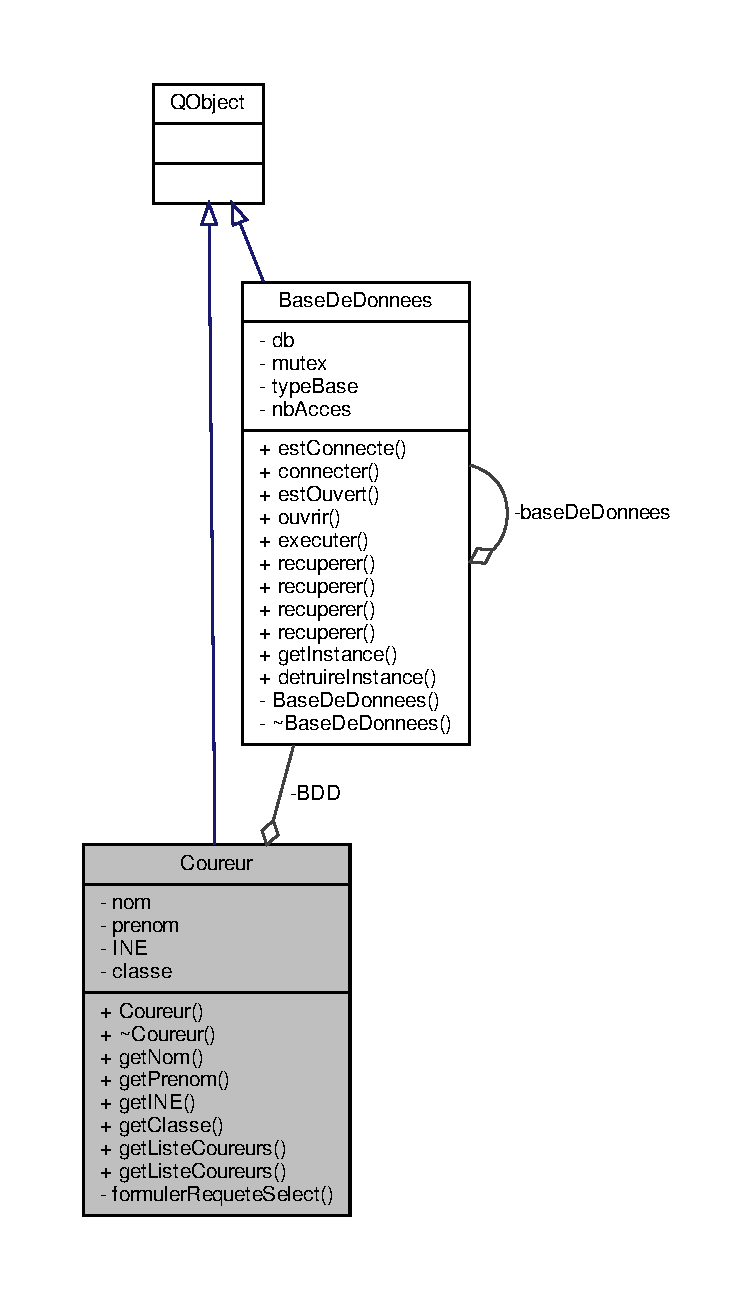
\includegraphics[height=550pt]{class_coureur__coll__graph}
\end{center}
\end{figure}
\subsubsection*{Connecteurs publics}
\begin{DoxyCompactItemize}
\item 
Q\+String\+List \hyperlink{class_coureur_a99e640aba229bb629e894729413b4e84}{get\+Liste\+Coureurs} (Q\+String, Q\+String, Q\+String, Q\+String)
\end{DoxyCompactItemize}
\subsubsection*{Fonctions membres publiques}
\begin{DoxyCompactItemize}
\item 
\hyperlink{class_coureur_af3a5607d96a0960b1666164f6a74d539}{Coureur} (\hyperlink{class_q_object}{Q\+Object} $\ast$parent=nullptr)
\begin{DoxyCompactList}\small\item\em \hyperlink{class_coureur}{Coureur}. \end{DoxyCompactList}\item 
\hyperlink{class_coureur_acbaa69246e4da18c0951f651f9ab3d69}{$\sim$\+Coureur} ()
\item 
Q\+String \hyperlink{class_coureur_a1808f13910638c6f2a57e87be522adf3}{get\+Nom} () const
\item 
Q\+String \hyperlink{class_coureur_a54a92a0fcaf7db9079f9d3f5d043539c}{get\+Prenom} () const
\item 
Q\+String \hyperlink{class_coureur_a724d13c5c34757fcd70491da44a918e3}{get\+I\+NE} () const
\item 
Q\+String \hyperlink{class_coureur_aa611e208767c4db4999e00296aa12632}{get\+Classe} () const
\item 
Q\+Vector$<$ Q\+String $>$ \hyperlink{class_coureur_a1d9f2cb15f74ff1c7b20fde081b5c5d6}{get\+Liste\+Coureurs} (Q\+String \hyperlink{class_coureur}{Coureur})
\end{DoxyCompactItemize}
\subsubsection*{Fonctions membres privées}
\begin{DoxyCompactItemize}
\item 
Q\+String \hyperlink{class_coureur_ad46f9151c1d00fbddb31c352ba331d78}{formuler\+Requete\+Select} (Q\+String renseignements, Q\+String sources, Q\+String conditions)
\end{DoxyCompactItemize}
\subsubsection*{Attributs privés}
\begin{DoxyCompactItemize}
\item 
Q\+String \hyperlink{class_coureur_ac96ff159efad8a6fd3abbe1a37b51c24}{nom}
\item 
Q\+String \hyperlink{class_coureur_a5e37d256b17765909423e183879c9e58}{prenom}
\item 
Q\+String \hyperlink{class_coureur_ac4028301fbd425848c2a81d69f8f94ac}{I\+NE}
\item 
Q\+String \hyperlink{class_coureur_a274255068bb91a5c66a365cd10528280}{classe}
\item 
\hyperlink{class_base_de_donnees}{Base\+De\+Donnees} $\ast$ \hyperlink{class_coureur_a9890c210d97e593644b22cb0e8228527}{B\+DD}
\begin{DoxyCompactList}\small\item\em agrégation \hyperlink{class_base_de_donnees}{Base\+De\+Donnees} \end{DoxyCompactList}\end{DoxyCompactItemize}


\subsubsection{Description détaillée}
Gérer les coureurs. 

\begin{DoxyAuthor}{Auteur}
Suzie Turlin
\end{DoxyAuthor}
\begin{DoxyVersion}{Version}
0.\+1 
\end{DoxyVersion}


\subsubsection{Documentation des constructeurs et destructeur}
\mbox{\Hypertarget{class_coureur_af3a5607d96a0960b1666164f6a74d539}\label{class_coureur_af3a5607d96a0960b1666164f6a74d539}} 
\index{Coureur@{Coureur}!Coureur@{Coureur}}
\index{Coureur@{Coureur}!Coureur@{Coureur}}
\paragraph{\texorpdfstring{Coureur()}{Coureur()}}
{\footnotesize\ttfamily Coureur\+::\+Coureur (\begin{DoxyParamCaption}\item[{\hyperlink{class_q_object}{Q\+Object} $\ast$}]{parent = {\ttfamily nullptr} }\end{DoxyParamCaption})\hspace{0.3cm}{\ttfamily [explicit]}}



\hyperlink{class_coureur}{Coureur}. 


\begin{DoxyParams}{Paramètres}
{\em parent} & \hyperlink{class_q_object}{Q\+Object} Adresse de l\textquotesingle{}objet Qt parent \\
\hline
\end{DoxyParams}


Références \hyperlink{class_coureur_a9890c210d97e593644b22cb0e8228527}{B\+DD}, \hyperlink{class_base_de_donnees_ab2e092285ccc0ee1cce61a1774218561}{Base\+De\+Donnees\+::connecter()}, \hyperlink{class_base_de_donnees_a00388973f3ec42e5c8e76e7af7e124b2}{Base\+De\+Donnees\+::est\+Connecte()}, et \hyperlink{class_base_de_donnees_a80028aa2b6b4fbf30fb2e36357b7d3d3}{Base\+De\+Donnees\+::get\+Instance()}.


\begin{DoxyCode}
00025                                 : \hyperlink{class_q_object}{QObject}(parent)
00026 \{
00027     \textcolor{comment}{//**TODO BASE DE DONNEE**//}
00028 
00029     \hyperlink{class_coureur_a9890c210d97e593644b22cb0e8228527}{BDD} = \hyperlink{class_base_de_donnees_a80028aa2b6b4fbf30fb2e36357b7d3d3}{BaseDeDonnees::getInstance}();
00030     \textcolor{keywordflow}{if}(!\hyperlink{class_coureur_a9890c210d97e593644b22cb0e8228527}{BDD}->\hyperlink{class_base_de_donnees_a00388973f3ec42e5c8e76e7af7e124b2}{estConnecte}())
00031         \hyperlink{class_coureur_a9890c210d97e593644b22cb0e8228527}{BDD}->\hyperlink{class_base_de_donnees_ab2e092285ccc0ee1cce61a1774218561}{connecter}(\textcolor{stringliteral}{"Resultats-Cross"});
00032     qDebug() << Q\_FUNC\_INFO << \textcolor{stringliteral}{"Etat connexion BDD : "} << \hyperlink{class_coureur_a9890c210d97e593644b22cb0e8228527}{BDD}->\hyperlink{class_base_de_donnees_a00388973f3ec42e5c8e76e7af7e124b2}{estConnecte}();
00033 
00034 
00035 \}
\end{DoxyCode}
\mbox{\Hypertarget{class_coureur_acbaa69246e4da18c0951f651f9ab3d69}\label{class_coureur_acbaa69246e4da18c0951f651f9ab3d69}} 
\index{Coureur@{Coureur}!````~Coureur@{$\sim$\+Coureur}}
\index{````~Coureur@{$\sim$\+Coureur}!Coureur@{Coureur}}
\paragraph{\texorpdfstring{$\sim$\+Coureur()}{~Coureur()}}
{\footnotesize\ttfamily Coureur\+::$\sim$\+Coureur (\begin{DoxyParamCaption}{ }\end{DoxyParamCaption})}


\begin{DoxyCode}
00038 \{
00039 
00040 \}
\end{DoxyCode}


\subsubsection{Documentation des fonctions membres}
\mbox{\Hypertarget{class_coureur_ad46f9151c1d00fbddb31c352ba331d78}\label{class_coureur_ad46f9151c1d00fbddb31c352ba331d78}} 
\index{Coureur@{Coureur}!formuler\+Requete\+Select@{formuler\+Requete\+Select}}
\index{formuler\+Requete\+Select@{formuler\+Requete\+Select}!Coureur@{Coureur}}
\paragraph{\texorpdfstring{formuler\+Requete\+Select()}{formulerRequeteSelect()}}
{\footnotesize\ttfamily Q\+String Coureur\+::formuler\+Requete\+Select (\begin{DoxyParamCaption}\item[{Q\+String}]{renseignements,  }\item[{Q\+String}]{sources,  }\item[{Q\+String}]{conditions }\end{DoxyParamCaption})\hspace{0.3cm}{\ttfamily [private]}}


\begin{DoxyCode}
00069 \{
00070     QString requete = QString(\textcolor{stringliteral}{"SELECT %1 FROM %2 WHERE %3"}).arg(renseignements).arg(sources).arg(conditions
      );
00071     qDebug() << Q\_FUNC\_INFO << \textcolor{stringliteral}{"Requête select : "} << requete;
00072     \textcolor{keywordflow}{return} requete;
00073 \}
\end{DoxyCode}
\mbox{\Hypertarget{class_coureur_aa611e208767c4db4999e00296aa12632}\label{class_coureur_aa611e208767c4db4999e00296aa12632}} 
\index{Coureur@{Coureur}!get\+Classe@{get\+Classe}}
\index{get\+Classe@{get\+Classe}!Coureur@{Coureur}}
\paragraph{\texorpdfstring{get\+Classe()}{getClasse()}}
{\footnotesize\ttfamily Q\+String Coureur\+::get\+Classe (\begin{DoxyParamCaption}{ }\end{DoxyParamCaption}) const}



Références \hyperlink{class_coureur_a274255068bb91a5c66a365cd10528280}{classe}.


\begin{DoxyCode}
00053 \{
00054     \textcolor{keywordflow}{return} \hyperlink{class_coureur_a274255068bb91a5c66a365cd10528280}{classe};
00055 \}
\end{DoxyCode}
\mbox{\Hypertarget{class_coureur_a724d13c5c34757fcd70491da44a918e3}\label{class_coureur_a724d13c5c34757fcd70491da44a918e3}} 
\index{Coureur@{Coureur}!get\+I\+NE@{get\+I\+NE}}
\index{get\+I\+NE@{get\+I\+NE}!Coureur@{Coureur}}
\paragraph{\texorpdfstring{get\+I\+N\+E()}{getINE()}}
{\footnotesize\ttfamily Q\+String Coureur\+::get\+I\+NE (\begin{DoxyParamCaption}{ }\end{DoxyParamCaption}) const}



Références \hyperlink{class_coureur_ac4028301fbd425848c2a81d69f8f94ac}{I\+NE}.


\begin{DoxyCode}
00058 \{
00059     \textcolor{keywordflow}{return} \hyperlink{class_coureur_ac4028301fbd425848c2a81d69f8f94ac}{INE};
00060 \}
\end{DoxyCode}
\mbox{\Hypertarget{class_coureur_a1d9f2cb15f74ff1c7b20fde081b5c5d6}\label{class_coureur_a1d9f2cb15f74ff1c7b20fde081b5c5d6}} 
\index{Coureur@{Coureur}!get\+Liste\+Coureurs@{get\+Liste\+Coureurs}}
\index{get\+Liste\+Coureurs@{get\+Liste\+Coureurs}!Coureur@{Coureur}}
\paragraph{\texorpdfstring{get\+Liste\+Coureurs()}{getListeCoureurs()}\hspace{0.1cm}{\footnotesize\ttfamily [1/2]}}
{\footnotesize\ttfamily Q\+Vector$<$Q\+String$>$ Coureur\+::get\+Liste\+Coureurs (\begin{DoxyParamCaption}\item[{Q\+String}]{Coureur }\end{DoxyParamCaption})}

\mbox{\Hypertarget{class_coureur_a99e640aba229bb629e894729413b4e84}\label{class_coureur_a99e640aba229bb629e894729413b4e84}} 
\index{Coureur@{Coureur}!get\+Liste\+Coureurs@{get\+Liste\+Coureurs}}
\index{get\+Liste\+Coureurs@{get\+Liste\+Coureurs}!Coureur@{Coureur}}
\paragraph{\texorpdfstring{get\+Liste\+Coureurs}{getListeCoureurs}\hspace{0.1cm}{\footnotesize\ttfamily [2/2]}}
{\footnotesize\ttfamily Q\+String\+List Coureur\+::get\+Liste\+Coureurs (\begin{DoxyParamCaption}\item[{Q\+String}]{,  }\item[{Q\+String}]{,  }\item[{Q\+String}]{,  }\item[{Q\+String}]{ }\end{DoxyParamCaption})\hspace{0.3cm}{\ttfamily [slot]}}

\mbox{\Hypertarget{class_coureur_a1808f13910638c6f2a57e87be522adf3}\label{class_coureur_a1808f13910638c6f2a57e87be522adf3}} 
\index{Coureur@{Coureur}!get\+Nom@{get\+Nom}}
\index{get\+Nom@{get\+Nom}!Coureur@{Coureur}}
\paragraph{\texorpdfstring{get\+Nom()}{getNom()}}
{\footnotesize\ttfamily Q\+String Coureur\+::get\+Nom (\begin{DoxyParamCaption}{ }\end{DoxyParamCaption}) const}



Références \hyperlink{class_coureur_ac96ff159efad8a6fd3abbe1a37b51c24}{nom}.


\begin{DoxyCode}
00043 \{
00044     \textcolor{keywordflow}{return} \hyperlink{class_coureur_ac96ff159efad8a6fd3abbe1a37b51c24}{nom};
00045 \}
\end{DoxyCode}
\mbox{\Hypertarget{class_coureur_a54a92a0fcaf7db9079f9d3f5d043539c}\label{class_coureur_a54a92a0fcaf7db9079f9d3f5d043539c}} 
\index{Coureur@{Coureur}!get\+Prenom@{get\+Prenom}}
\index{get\+Prenom@{get\+Prenom}!Coureur@{Coureur}}
\paragraph{\texorpdfstring{get\+Prenom()}{getPrenom()}}
{\footnotesize\ttfamily Q\+String Coureur\+::get\+Prenom (\begin{DoxyParamCaption}{ }\end{DoxyParamCaption}) const}



Références \hyperlink{class_coureur_a5e37d256b17765909423e183879c9e58}{prenom}.


\begin{DoxyCode}
00048 \{
00049     \textcolor{keywordflow}{return} \hyperlink{class_coureur_a5e37d256b17765909423e183879c9e58}{prenom};
00050 \}
\end{DoxyCode}


\subsubsection{Documentation des données membres}
\mbox{\Hypertarget{class_coureur_a9890c210d97e593644b22cb0e8228527}\label{class_coureur_a9890c210d97e593644b22cb0e8228527}} 
\index{Coureur@{Coureur}!B\+DD@{B\+DD}}
\index{B\+DD@{B\+DD}!Coureur@{Coureur}}
\paragraph{\texorpdfstring{B\+DD}{BDD}}
{\footnotesize\ttfamily \hyperlink{class_base_de_donnees}{Base\+De\+Donnees}$\ast$ Coureur\+::\+B\+DD\hspace{0.3cm}{\ttfamily [private]}}



agrégation \hyperlink{class_base_de_donnees}{Base\+De\+Donnees} 



Référencé par \hyperlink{class_coureur_af3a5607d96a0960b1666164f6a74d539}{Coureur()}.

\mbox{\Hypertarget{class_coureur_a274255068bb91a5c66a365cd10528280}\label{class_coureur_a274255068bb91a5c66a365cd10528280}} 
\index{Coureur@{Coureur}!classe@{classe}}
\index{classe@{classe}!Coureur@{Coureur}}
\paragraph{\texorpdfstring{classe}{classe}}
{\footnotesize\ttfamily Q\+String Coureur\+::classe\hspace{0.3cm}{\ttfamily [private]}}



Référencé par \hyperlink{class_coureur_aa611e208767c4db4999e00296aa12632}{get\+Classe()}.

\mbox{\Hypertarget{class_coureur_ac4028301fbd425848c2a81d69f8f94ac}\label{class_coureur_ac4028301fbd425848c2a81d69f8f94ac}} 
\index{Coureur@{Coureur}!I\+NE@{I\+NE}}
\index{I\+NE@{I\+NE}!Coureur@{Coureur}}
\paragraph{\texorpdfstring{I\+NE}{INE}}
{\footnotesize\ttfamily Q\+String Coureur\+::\+I\+NE\hspace{0.3cm}{\ttfamily [private]}}



Référencé par \hyperlink{class_coureur_a724d13c5c34757fcd70491da44a918e3}{get\+I\+N\+E()}.

\mbox{\Hypertarget{class_coureur_ac96ff159efad8a6fd3abbe1a37b51c24}\label{class_coureur_ac96ff159efad8a6fd3abbe1a37b51c24}} 
\index{Coureur@{Coureur}!nom@{nom}}
\index{nom@{nom}!Coureur@{Coureur}}
\paragraph{\texorpdfstring{nom}{nom}}
{\footnotesize\ttfamily Q\+String Coureur\+::nom\hspace{0.3cm}{\ttfamily [private]}}



Référencé par \hyperlink{class_coureur_a1808f13910638c6f2a57e87be522adf3}{get\+Nom()}.

\mbox{\Hypertarget{class_coureur_a5e37d256b17765909423e183879c9e58}\label{class_coureur_a5e37d256b17765909423e183879c9e58}} 
\index{Coureur@{Coureur}!prenom@{prenom}}
\index{prenom@{prenom}!Coureur@{Coureur}}
\paragraph{\texorpdfstring{prenom}{prenom}}
{\footnotesize\ttfamily Q\+String Coureur\+::prenom\hspace{0.3cm}{\ttfamily [private]}}



Référencé par \hyperlink{class_coureur_a54a92a0fcaf7db9079f9d3f5d043539c}{get\+Prenom()}.



La documentation de cette classe a été générée à partir des fichiers suivants \+:\begin{DoxyCompactItemize}
\item 
\hyperlink{coureur_8h}{coureur.\+h}\item 
\hyperlink{coureur_8cpp}{coureur.\+cpp}\end{DoxyCompactItemize}

\hypertarget{class_course}{}\subsection{Référence de la classe Course}
\label{class_course}\index{Course@{Course}}


Déclaration de la classe \hyperlink{class_course}{Course}.  




{\ttfamily \#include $<$course.\+h$>$}



Graphe de collaboration de Course\+:\nopagebreak
\begin{figure}[H]
\begin{center}
\leavevmode
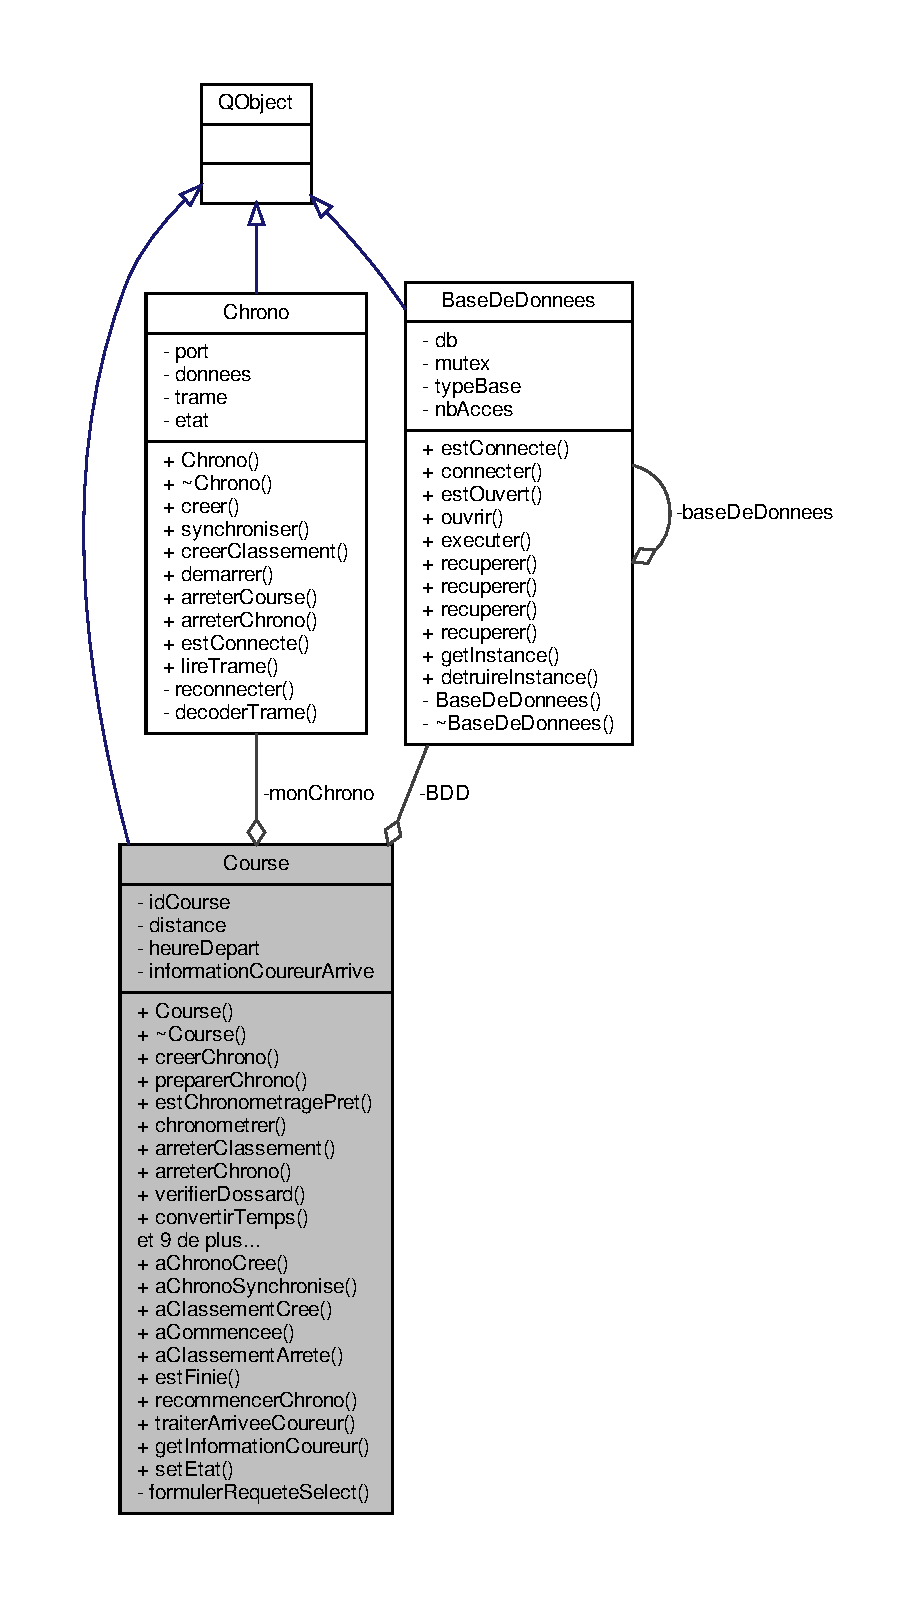
\includegraphics[height=550pt]{class_course__coll__graph}
\end{center}
\end{figure}
\subsubsection*{Connecteurs publics}
\begin{DoxyCompactItemize}
\item 
void \hyperlink{class_course_ada484058a0180a31a98ee77c4fad93f8}{a\+Chrono\+Cree} ()
\begin{DoxyCompactList}\small\item\em S\+L\+OT \hyperlink{class_course_ada484058a0180a31a98ee77c4fad93f8}{a\+Chrono\+Cree()} de la classe \hyperlink{class_course}{Course}. \end{DoxyCompactList}\item 
void \hyperlink{class_course_a90c66d620f0726d92c40069f052e0cd0}{a\+Chrono\+Synchronise} ()
\begin{DoxyCompactList}\small\item\em S\+L\+OT \hyperlink{class_course_a90c66d620f0726d92c40069f052e0cd0}{a\+Chrono\+Synchronise()} de la classe \hyperlink{class_course}{Course}. \end{DoxyCompactList}\item 
void \hyperlink{class_course_a4a4f788b4ff5ca687c67f29753d26928}{a\+Classement\+Cree} ()
\begin{DoxyCompactList}\small\item\em S\+L\+OT a\+Classement\+Cree de la classe \hyperlink{class_course}{Course}. \end{DoxyCompactList}\item 
void \hyperlink{class_course_a8df970d7150703c3279903b09aa38855}{a\+Commencee} ()
\begin{DoxyCompactList}\small\item\em S\+L\+OT \hyperlink{class_course_a8df970d7150703c3279903b09aa38855}{a\+Commencee()} de la classe \hyperlink{class_course}{Course}. \end{DoxyCompactList}\item 
void \hyperlink{class_course_a43696137587262b721767f6113621772}{a\+Classement\+Arrete} ()
\begin{DoxyCompactList}\small\item\em S\+L\+OT \hyperlink{class_course_a43696137587262b721767f6113621772}{a\+Classement\+Arrete()} de la classe \hyperlink{class_course}{Course}. \end{DoxyCompactList}\item 
void \hyperlink{class_course_abbcfaecd40b5ec5e47419068423e767f}{est\+Finie} ()
\begin{DoxyCompactList}\small\item\em S\+L\+OT \hyperlink{class_course_abbcfaecd40b5ec5e47419068423e767f}{est\+Finie()} de la classe \hyperlink{class_course}{Course}. \end{DoxyCompactList}\item 
void \hyperlink{class_course_addeae907c4bc0a268f51479041de389c}{recommencer\+Chrono} ()
\begin{DoxyCompactList}\small\item\em S\+L\+OT \hyperlink{class_course_addeae907c4bc0a268f51479041de389c}{recommencer\+Chrono()} de la classe \hyperlink{class_course}{Course}. \end{DoxyCompactList}\item 
void \hyperlink{class_course_a60073d16efd4ccefa81bddb4aaa88fab}{traiter\+Arrivee\+Coureur} (Q\+String temps\+Arrivee)
\begin{DoxyCompactList}\small\item\em S\+L\+OT \hyperlink{class_course_a60073d16efd4ccefa81bddb4aaa88fab}{traiter\+Arrivee\+Coureur(\+Q\+String temps\+Arrivee)} de la classe \hyperlink{class_course}{Course}. \end{DoxyCompactList}\item 
void \hyperlink{class_course_a7ba5d2c9865065e95f49a24fbeec7857}{get\+Information\+Coureur} (Q\+String dossard, Q\+String temps\+A\+Rrivee)
\begin{DoxyCompactList}\small\item\em S\+L\+OT \hyperlink{class_course_a7ba5d2c9865065e95f49a24fbeec7857}{get\+Information\+Coureur(\+Q\+String dossard, Q\+String temps\+Arrivee)} de la classe \hyperlink{class_course}{Course}. \end{DoxyCompactList}\item 
bool \hyperlink{class_course_a3ebcde1fa443cb20d71fb98af4d0c418}{set\+Etat} (Q\+String etat)
\begin{DoxyCompactList}\small\item\em S\+L\+OT set\+Etat de la classe \hyperlink{class_course}{Course}. \end{DoxyCompactList}\end{DoxyCompactItemize}
\subsubsection*{Signaux}
\begin{DoxyCompactItemize}
\item 
void \hyperlink{class_course_a1c7830a51af59f70998ff0576f0aa7cd}{chrono\+Creer} ()
\item 
void \hyperlink{class_course_ab3f2a2c1bb8ed8a2550dc8fabc59e54e}{chrono\+Course\+Pret} ()
\item 
void \hyperlink{class_course_a2056f5c20f56e2c7eeea8195a55857bc}{course\+Commence} ()
\item 
void \hyperlink{class_course_a630aea833dccd20e52ada1548c334c78}{classement\+Arrete} ()
\item 
void \hyperlink{class_course_aa66c89bb34e692f17caabb21b11feeb2}{course\+Finie} ()
\item 
void \hyperlink{class_course_a178f2015d20ef5d838564671567f6831}{chrono\+Recommence} ()
\item 
void \hyperlink{class_course_abea30de9b6cec333bf19134608e5bccf}{nouveau\+Temps\+Arrivee} (Q\+String temps\+Arrivee)
\item 
void \hyperlink{class_course_aa2f0312e68f57e1437c3257d13af8186}{arrivee\+Ajoutee\+B\+DD} (Q\+String dossard, Q\+String temps\+Arrivee)
\item 
void \hyperlink{class_course_a9073b7cb57b9b8a2aee33582bb61eb20}{information\+Coureur\+Recuperees} (Q\+String\+List information\+Coureur)
\end{DoxyCompactItemize}
\subsubsection*{Fonctions membres publiques}
\begin{DoxyCompactItemize}
\item 
\hyperlink{class_course_af6317ecab95f8a2eb205b4f91b530992}{Course} (\hyperlink{class_q_object}{Q\+Object} $\ast$parent=nullptr)
\begin{DoxyCompactList}\small\item\em Constructeur de la classe \hyperlink{class_course}{Course}. \end{DoxyCompactList}\item 
\hyperlink{class_course_aa9038f2e129526920037dda9e76d69d0}{$\sim$\+Course} ()
\begin{DoxyCompactList}\small\item\em Destructeur de la fenêtre principale. \end{DoxyCompactList}\item 
void \hyperlink{class_course_a6eb96222d8dc1f352e28f36e9b414448}{creer\+Chrono} ()
\begin{DoxyCompactList}\small\item\em Méthode \hyperlink{class_course_a6eb96222d8dc1f352e28f36e9b414448}{creer\+Chrono()} de la classe \hyperlink{class_course}{Course}. \end{DoxyCompactList}\item 
void \hyperlink{class_course_a50596f54553b48fa29170a6b42b6e9d4}{preparer\+Chrono} ()
\begin{DoxyCompactList}\small\item\em Méthode \hyperlink{class_course_a50596f54553b48fa29170a6b42b6e9d4}{preparer\+Chrono()} de la classe \hyperlink{class_course}{Course}. \end{DoxyCompactList}\item 
bool \hyperlink{class_course_a44a14d431bd64a507f2c2aa5f465b1b0}{est\+Chronometrage\+Pret} ()
\begin{DoxyCompactList}\small\item\em Méthode \hyperlink{class_course_a44a14d431bd64a507f2c2aa5f465b1b0}{est\+Chronometrage\+Pret()} de la classe \hyperlink{class_course}{Course}. \end{DoxyCompactList}\item 
void \hyperlink{class_course_a589447dd63dca89395119ffd4e4a8c8c}{chronometrer} ()
\begin{DoxyCompactList}\small\item\em Méthode chronometrer de la classe \hyperlink{class_course}{Course}. \end{DoxyCompactList}\item 
void \hyperlink{class_course_a4426310a411d8ecf7f4a2dc64c24a42d}{arreter\+Classement} ()
\begin{DoxyCompactList}\small\item\em Méthode \hyperlink{class_course_a4426310a411d8ecf7f4a2dc64c24a42d}{arreter\+Classement()} de la classe \hyperlink{class_course}{Course}. \end{DoxyCompactList}\item 
void \hyperlink{class_course_a939635ac8301a7018475cc2ce347375f}{arreter\+Chrono} ()
\begin{DoxyCompactList}\small\item\em Méthode arreter\+Chronomètre() de la classe \hyperlink{class_course}{Course}. \end{DoxyCompactList}\item 
int \hyperlink{class_course_a6cb3ede6a11e4813f95be92f4459a3c2}{verifier\+Dossard} (Q\+String dossard)
\begin{DoxyCompactList}\small\item\em Méthode \hyperlink{class_course_a6cb3ede6a11e4813f95be92f4459a3c2}{verifier\+Dossard()} de la classe \hyperlink{class_course}{Course}. \end{DoxyCompactList}\item 
Q\+String \hyperlink{class_course_ab98bbd1a92e468df7b8b45bb7877afef}{convertir\+Temps} (Q\+String temps\+MS)
\begin{DoxyCompactList}\small\item\em Méthode \hyperlink{class_course_ab98bbd1a92e468df7b8b45bb7877afef}{convertir\+Temps()} de la classe \hyperlink{class_course}{Course}. \end{DoxyCompactList}\item 
int \hyperlink{class_course_ad0ff4153f1e02826d551f478f95ad260}{get\+Nb\+Inscrit} (Q\+String course)
\begin{DoxyCompactList}\small\item\em Méthode get\+Nb\+Inscrit de la classe \hyperlink{class_course}{Course}. \end{DoxyCompactList}\item 
int \hyperlink{class_course_af20fcd6d6eb2dfbd3b0f12e273f12b27}{get\+Distance} (Q\+String course)
\begin{DoxyCompactList}\small\item\em Méthode \hyperlink{class_course_af20fcd6d6eb2dfbd3b0f12e273f12b27}{get\+Distance()} de la classe \hyperlink{class_course}{Course}. \end{DoxyCompactList}\item 
Q\+String \hyperlink{class_course_afc21f8195edd50c9fd266cff0c401b7c}{get\+Heure} (Q\+String course)
\begin{DoxyCompactList}\small\item\em Méthode \hyperlink{class_course_afc21f8195edd50c9fd266cff0c401b7c}{get\+Heure()} de la classe \hyperlink{class_course}{Course}. \end{DoxyCompactList}\item 
int \hyperlink{class_course_ad8dd87e7f299bc938f40423f28c837e8}{get\+Nb\+Arrivee} ()
\begin{DoxyCompactList}\small\item\em Méthode \hyperlink{class_course_ad8dd87e7f299bc938f40423f28c837e8}{get\+Nb\+Arrivee()} de la classe \hyperlink{class_course}{Course}. \end{DoxyCompactList}\item 
Q\+String \hyperlink{class_course_a7b4485a0b38bc3b908131962b705d880}{get\+Nom\+Course} (Q\+String dossard)
\begin{DoxyCompactList}\small\item\em Méthode \hyperlink{class_course_a7b4485a0b38bc3b908131962b705d880}{get\+Nom\+Course()} de la classe \hyperlink{class_course}{Course}. \end{DoxyCompactList}\item 
void \hyperlink{class_course_a36cf16c971841431947b6fbe2b3f3d27}{set\+Id\+Course} (Q\+String nom\+Course)
\begin{DoxyCompactList}\small\item\em Méthode \hyperlink{class_course_a36cf16c971841431947b6fbe2b3f3d27}{set\+Id\+Course()} de la classe \hyperlink{class_course}{Course}. \end{DoxyCompactList}\item 
void \hyperlink{class_course_ac99042bf8b20e8d3a54e72c8a80f7ee7}{ajoute\+Arrivee\+B\+DD} (Q\+String dossard, Q\+String temps\+Arrivee)
\begin{DoxyCompactList}\small\item\em Méthode \hyperlink{class_course_ac99042bf8b20e8d3a54e72c8a80f7ee7}{ajoute\+Arrivee\+B\+D\+D()} de la classe \hyperlink{class_course}{Course}. \end{DoxyCompactList}\item 
Q\+String\+List \hyperlink{class_course_a0d995ef72152208e02eb3b10315dfabb}{get\+Liste\+Manifestations} ()
\begin{DoxyCompactList}\small\item\em Méthode \hyperlink{class_course_a0d995ef72152208e02eb3b10315dfabb}{get\+Liste\+Manifestations()} de la classe \hyperlink{class_course}{Course}. \end{DoxyCompactList}\item 
Q\+Vector$<$ Q\+String $>$ \hyperlink{class_course_ae5e74946d973166ad3000e38600acf20}{get\+Liste\+Courses} (Q\+String manifestation)
\begin{DoxyCompactList}\small\item\em Méthode \hyperlink{class_course_ae5e74946d973166ad3000e38600acf20}{get\+Liste\+Courses()} de la classe \hyperlink{class_course}{Course}. \end{DoxyCompactList}\end{DoxyCompactItemize}
\subsubsection*{Fonctions membres privées}
\begin{DoxyCompactItemize}
\item 
Q\+String \hyperlink{class_course_a2ce9c62ead2c878a30af9d9c11b81644}{formuler\+Requete\+Select} (Q\+String renseignements, Q\+String sources, Q\+String conditions)
\begin{DoxyCompactList}\small\item\em Méthode formuler\+Requete\+Select de la classe \hyperlink{class_course}{Course}. \end{DoxyCompactList}\end{DoxyCompactItemize}
\subsubsection*{Attributs privés}
\begin{DoxyCompactItemize}
\item 
\hyperlink{class_base_de_donnees}{Base\+De\+Donnees} $\ast$ \hyperlink{class_course_a28a58b06494361b7a7eb81844d571dd4}{B\+DD}
\begin{DoxyCompactList}\small\item\em agrégation \hyperlink{class_base_de_donnees}{Base\+De\+Donnees} \end{DoxyCompactList}\item 
\hyperlink{class_chrono}{Chrono} $\ast$ \hyperlink{class_course_a0c9b246b0f1ec612bd6e6c613a94d52b}{mon\+Chrono}
\begin{DoxyCompactList}\small\item\em association \hyperlink{class_chrono}{Chrono} \end{DoxyCompactList}\item 
Q\+String \hyperlink{class_course_a1f80798e50be6db9911a882a2491c698}{id\+Course}
\begin{DoxyCompactList}\small\item\em Identifiant de la course. \end{DoxyCompactList}\item 
Q\+String \hyperlink{class_course_af2f7b814a0ec0d76291a2743c61615a8}{distance}
\begin{DoxyCompactList}\small\item\em Distance de la course. \end{DoxyCompactList}\item 
Q\+String \hyperlink{class_course_aa2da10dd2fc8c1ca1d5831249181e61f}{heure\+Depart}
\begin{DoxyCompactList}\small\item\em L\textquotesingle{}heure de départ de la course. \end{DoxyCompactList}\item 
Q\+String\+List \hyperlink{class_course_a14838cc0c491a76baf7e5f12d8d08ab4}{information\+Coureur\+Arrive}
\begin{DoxyCompactList}\small\item\em Informations d\textquotesingle{}un coure. \end{DoxyCompactList}\end{DoxyCompactItemize}


\subsubsection{Description détaillée}
Déclaration de la classe \hyperlink{class_course}{Course}. 

\begin{DoxyAuthor}{Auteur}
Michael Andréo 
\end{DoxyAuthor}
\begin{DoxyVersion}{Version}
1.\+1 
\end{DoxyVersion}


\subsubsection{Documentation des constructeurs et destructeur}
\mbox{\Hypertarget{class_course_af6317ecab95f8a2eb205b4f91b530992}\label{class_course_af6317ecab95f8a2eb205b4f91b530992}} 
\index{Course@{Course}!Course@{Course}}
\index{Course@{Course}!Course@{Course}}
\paragraph{\texorpdfstring{Course()}{Course()}}
{\footnotesize\ttfamily Course\+::\+Course (\begin{DoxyParamCaption}\item[{\hyperlink{class_q_object}{Q\+Object} $\ast$}]{parent = {\ttfamily nullptr} }\end{DoxyParamCaption})}



Constructeur de la classe \hyperlink{class_course}{Course}. 


\begin{DoxyParams}{Paramètres}
{\em parent} & \hyperlink{class_q_object}{Q\+Object} Adresse de l\textquotesingle{}objet Qt parent (0 = pas de parent car c\textquotesingle{}est la fenêtre principale) \\
\hline
\end{DoxyParams}


Références \hyperlink{class_course_ada484058a0180a31a98ee77c4fad93f8}{a\+Chrono\+Cree()}, \hyperlink{class_course_a90c66d620f0726d92c40069f052e0cd0}{a\+Chrono\+Synchronise()}, \hyperlink{class_course_a43696137587262b721767f6113621772}{a\+Classement\+Arrete()}, \hyperlink{class_course_a4a4f788b4ff5ca687c67f29753d26928}{a\+Classement\+Cree()}, \hyperlink{class_course_a8df970d7150703c3279903b09aa38855}{a\+Commencee()}, \hyperlink{class_course_aa2f0312e68f57e1437c3257d13af8186}{arrivee\+Ajoutee\+B\+D\+D()}, \hyperlink{class_course_a28a58b06494361b7a7eb81844d571dd4}{B\+DD}, \hyperlink{class_course_a1c7830a51af59f70998ff0576f0aa7cd}{chrono\+Creer()}, \hyperlink{class_course_a178f2015d20ef5d838564671567f6831}{chrono\+Recommence()}, \hyperlink{class_base_de_donnees_ab2e092285ccc0ee1cce61a1774218561}{Base\+De\+Donnees\+::connecter()}, \hyperlink{class_base_de_donnees_a00388973f3ec42e5c8e76e7af7e124b2}{Base\+De\+Donnees\+::est\+Connecte()}, \hyperlink{class_course_abbcfaecd40b5ec5e47419068423e767f}{est\+Finie()}, \hyperlink{class_course_a7ba5d2c9865065e95f49a24fbeec7857}{get\+Information\+Coureur()}, \hyperlink{class_base_de_donnees_a80028aa2b6b4fbf30fb2e36357b7d3d3}{Base\+De\+Donnees\+::get\+Instance()}, \hyperlink{class_course_a0c9b246b0f1ec612bd6e6c613a94d52b}{mon\+Chrono}, \hyperlink{class_course_addeae907c4bc0a268f51479041de389c}{recommencer\+Chrono()}, et \hyperlink{class_course_a60073d16efd4ccefa81bddb4aaa88fab}{traiter\+Arrivee\+Coureur()}.


\begin{DoxyCode}
00015                               : \hyperlink{class_q_object}{QObject}(parent)
00016 \{
00017     \hyperlink{class_course_a28a58b06494361b7a7eb81844d571dd4}{BDD} = \hyperlink{class_base_de_donnees_a80028aa2b6b4fbf30fb2e36357b7d3d3}{BaseDeDonnees::getInstance}();
00018     \textcolor{keywordflow}{if}(!\hyperlink{class_course_a28a58b06494361b7a7eb81844d571dd4}{BDD}->\hyperlink{class_base_de_donnees_a00388973f3ec42e5c8e76e7af7e124b2}{estConnecte}())
00019         \hyperlink{class_course_a28a58b06494361b7a7eb81844d571dd4}{BDD}->\hyperlink{class_base_de_donnees_ab2e092285ccc0ee1cce61a1774218561}{connecter}(\textcolor{stringliteral}{"Chrono-Cross"});
00020     qDebug() << Q\_FUNC\_INFO << \textcolor{stringliteral}{"Etat connexion BDD : "} << \hyperlink{class_course_a28a58b06494361b7a7eb81844d571dd4}{BDD}->\hyperlink{class_base_de_donnees_a00388973f3ec42e5c8e76e7af7e124b2}{estConnecte}();
00021 
00022     \hyperlink{class_course_a0c9b246b0f1ec612bd6e6c613a94d52b}{monChrono} = \textcolor{keyword}{new} \hyperlink{class_chrono}{Chrono}(\textcolor{keyword}{this});
00023 
00024     connect(\hyperlink{class_course_a0c9b246b0f1ec612bd6e6c613a94d52b}{monChrono}, SIGNAL(\hyperlink{class_course_a1c7830a51af59f70998ff0576f0aa7cd}{chronoCreer}()), \textcolor{keyword}{this}, SLOT(
      \hyperlink{class_course_ada484058a0180a31a98ee77c4fad93f8}{aChronoCree}()));
00025     connect(\hyperlink{class_course_a0c9b246b0f1ec612bd6e6c613a94d52b}{monChrono}, SIGNAL(chronoSynchroniser()), \textcolor{keyword}{this}, SLOT(
      \hyperlink{class_course_a90c66d620f0726d92c40069f052e0cd0}{aChronoSynchronise}()));
00026     connect(\hyperlink{class_course_a0c9b246b0f1ec612bd6e6c613a94d52b}{monChrono}, SIGNAL(classementCree()), \textcolor{keyword}{this}, SLOT(
      \hyperlink{class_course_a4a4f788b4ff5ca687c67f29753d26928}{aClassementCree}()));
00027     connect(\hyperlink{class_course_a0c9b246b0f1ec612bd6e6c613a94d52b}{monChrono}, SIGNAL(chronoLance()), \textcolor{keyword}{this}, SLOT(\hyperlink{class_course_a8df970d7150703c3279903b09aa38855}{aCommencee}()));
00028     connect(\hyperlink{class_course_a0c9b246b0f1ec612bd6e6c613a94d52b}{monChrono}, SIGNAL(courseArretee()), \textcolor{keyword}{this}, SLOT(
      \hyperlink{class_course_a43696137587262b721767f6113621772}{aClassementArrete}()));
00029     connect(\hyperlink{class_course_a0c9b246b0f1ec612bd6e6c613a94d52b}{monChrono}, SIGNAL(chronoArrete()), \textcolor{keyword}{this}, SLOT(\hyperlink{class_course_abbcfaecd40b5ec5e47419068423e767f}{estFinie}()));
00030     connect(\hyperlink{class_course_a0c9b246b0f1ec612bd6e6c613a94d52b}{monChrono}, SIGNAL(nouvelleArrivee(QString)), \textcolor{keyword}{this}, SLOT(
      \hyperlink{class_course_a60073d16efd4ccefa81bddb4aaa88fab}{traiterArriveeCoureur}(QString)));
00031     connect(\hyperlink{class_course_a0c9b246b0f1ec612bd6e6c613a94d52b}{monChrono}, SIGNAL(\hyperlink{class_course_a178f2015d20ef5d838564671567f6831}{chronoRecommence}()), \textcolor{keyword}{this}, SLOT(
      \hyperlink{class_course_addeae907c4bc0a268f51479041de389c}{recommencerChrono}()));
00032     connect(\textcolor{keyword}{this}, SIGNAL(\hyperlink{class_course_aa2f0312e68f57e1437c3257d13af8186}{arriveeAjouteeBDD}(QString, QString)), \textcolor{keyword}{this}, SLOT(
      \hyperlink{class_course_a7ba5d2c9865065e95f49a24fbeec7857}{getInformationCoureur}(QString, QString)));
00033 \}
\end{DoxyCode}
\mbox{\Hypertarget{class_course_aa9038f2e129526920037dda9e76d69d0}\label{class_course_aa9038f2e129526920037dda9e76d69d0}} 
\index{Course@{Course}!````~Course@{$\sim$\+Course}}
\index{````~Course@{$\sim$\+Course}!Course@{Course}}
\paragraph{\texorpdfstring{$\sim$\+Course()}{~Course()}}
{\footnotesize\ttfamily Course\+::$\sim$\+Course (\begin{DoxyParamCaption}{ }\end{DoxyParamCaption})}



Destructeur de la fenêtre principale. 



Références \hyperlink{class_base_de_donnees_a457401c0816b888c77ce915997545f4e}{Base\+De\+Donnees\+::detruire\+Instance()}.


\begin{DoxyCode}
00040 \{
00041     \hyperlink{class_base_de_donnees_a457401c0816b888c77ce915997545f4e}{BaseDeDonnees::detruireInstance}();
00042     qDebug() << Q\_FUNC\_INFO;
00043 \}
\end{DoxyCode}


\subsubsection{Documentation des fonctions membres}
\mbox{\Hypertarget{class_course_ada484058a0180a31a98ee77c4fad93f8}\label{class_course_ada484058a0180a31a98ee77c4fad93f8}} 
\index{Course@{Course}!a\+Chrono\+Cree@{a\+Chrono\+Cree}}
\index{a\+Chrono\+Cree@{a\+Chrono\+Cree}!Course@{Course}}
\paragraph{\texorpdfstring{a\+Chrono\+Cree}{aChronoCree}}
{\footnotesize\ttfamily void Course\+::a\+Chrono\+Cree (\begin{DoxyParamCaption}{ }\end{DoxyParamCaption})\hspace{0.3cm}{\ttfamily [slot]}}



S\+L\+OT \hyperlink{class_course_ada484058a0180a31a98ee77c4fad93f8}{a\+Chrono\+Cree()} de la classe \hyperlink{class_course}{Course}. 

Emet le signal chrono\+Creer 

Références \hyperlink{class_course_a1c7830a51af59f70998ff0576f0aa7cd}{chrono\+Creer()}.



Référencé par \hyperlink{class_course_af6317ecab95f8a2eb205b4f91b530992}{Course()}.


\begin{DoxyCode}
00467 \{
00468     emit \hyperlink{class_course_a1c7830a51af59f70998ff0576f0aa7cd}{chronoCreer}();
00469 \}
\end{DoxyCode}
\mbox{\Hypertarget{class_course_a90c66d620f0726d92c40069f052e0cd0}\label{class_course_a90c66d620f0726d92c40069f052e0cd0}} 
\index{Course@{Course}!a\+Chrono\+Synchronise@{a\+Chrono\+Synchronise}}
\index{a\+Chrono\+Synchronise@{a\+Chrono\+Synchronise}!Course@{Course}}
\paragraph{\texorpdfstring{a\+Chrono\+Synchronise}{aChronoSynchronise}}
{\footnotesize\ttfamily void Course\+::a\+Chrono\+Synchronise (\begin{DoxyParamCaption}{ }\end{DoxyParamCaption})\hspace{0.3cm}{\ttfamily [slot]}}



S\+L\+OT \hyperlink{class_course_a90c66d620f0726d92c40069f052e0cd0}{a\+Chrono\+Synchronise()} de la classe \hyperlink{class_course}{Course}. 

Appelle la méthode creer\+Classement() de la classe \hyperlink{class_chrono}{Chrono} 

Références \hyperlink{class_chrono_a0d7e3e50fcef0f2b0b7bfadc3d4f737d}{Chrono\+::creer\+Classement()}, et \hyperlink{class_course_a0c9b246b0f1ec612bd6e6c613a94d52b}{mon\+Chrono}.



Référencé par \hyperlink{class_course_af6317ecab95f8a2eb205b4f91b530992}{Course()}.


\begin{DoxyCode}
00477 \{
00478     \textcolor{keywordflow}{if}(\hyperlink{class_course_a0c9b246b0f1ec612bd6e6c613a94d52b}{monChrono}->\hyperlink{class_chrono_a0d7e3e50fcef0f2b0b7bfadc3d4f737d}{creerClassement}())
00479         qDebug() << Q\_FUNC\_INFO << \textcolor{stringliteral}{"NouveauClassement OK"};
00480     \textcolor{keywordflow}{else}
00481         qDebug() << Q\_FUNC\_INFO << \textcolor{stringliteral}{"ERREUR"};
00482 \}
\end{DoxyCode}
\mbox{\Hypertarget{class_course_a43696137587262b721767f6113621772}\label{class_course_a43696137587262b721767f6113621772}} 
\index{Course@{Course}!a\+Classement\+Arrete@{a\+Classement\+Arrete}}
\index{a\+Classement\+Arrete@{a\+Classement\+Arrete}!Course@{Course}}
\paragraph{\texorpdfstring{a\+Classement\+Arrete}{aClassementArrete}}
{\footnotesize\ttfamily void Course\+::a\+Classement\+Arrete (\begin{DoxyParamCaption}{ }\end{DoxyParamCaption})\hspace{0.3cm}{\ttfamily [slot]}}



S\+L\+OT \hyperlink{class_course_a43696137587262b721767f6113621772}{a\+Classement\+Arrete()} de la classe \hyperlink{class_course}{Course}. 

Emet le signal classement\+Arrete 

Références \hyperlink{class_course_a630aea833dccd20e52ada1548c334c78}{classement\+Arrete()}.



Référencé par \hyperlink{class_course_af6317ecab95f8a2eb205b4f91b530992}{Course()}.


\begin{DoxyCode}
00512 \{
00513     qDebug() << Q\_FUNC\_INFO << \textcolor{stringliteral}{"classement est arrété"};
00514     emit \hyperlink{class_course_a630aea833dccd20e52ada1548c334c78}{classementArrete}();
00515 \}
\end{DoxyCode}
\mbox{\Hypertarget{class_course_a4a4f788b4ff5ca687c67f29753d26928}\label{class_course_a4a4f788b4ff5ca687c67f29753d26928}} 
\index{Course@{Course}!a\+Classement\+Cree@{a\+Classement\+Cree}}
\index{a\+Classement\+Cree@{a\+Classement\+Cree}!Course@{Course}}
\paragraph{\texorpdfstring{a\+Classement\+Cree}{aClassementCree}}
{\footnotesize\ttfamily void Course\+::a\+Classement\+Cree (\begin{DoxyParamCaption}{ }\end{DoxyParamCaption})\hspace{0.3cm}{\ttfamily [slot]}}



S\+L\+OT a\+Classement\+Cree de la classe \hyperlink{class_course}{Course}. 

Permet de signaler à la classe I\+HM que le chronomètre de la course est pret. 

Références \hyperlink{class_course_ab3f2a2c1bb8ed8a2550dc8fabc59e54e}{chrono\+Course\+Pret()}.



Référencé par \hyperlink{class_course_af6317ecab95f8a2eb205b4f91b530992}{Course()}.


\begin{DoxyCode}
00490 \{
00491     qDebug() << Q\_FUNC\_INFO << \textcolor{stringliteral}{"Chrono pret"};
00492     emit \hyperlink{class_course_ab3f2a2c1bb8ed8a2550dc8fabc59e54e}{chronoCoursePret}();
00493 \}
\end{DoxyCode}
\mbox{\Hypertarget{class_course_a8df970d7150703c3279903b09aa38855}\label{class_course_a8df970d7150703c3279903b09aa38855}} 
\index{Course@{Course}!a\+Commencee@{a\+Commencee}}
\index{a\+Commencee@{a\+Commencee}!Course@{Course}}
\paragraph{\texorpdfstring{a\+Commencee}{aCommencee}}
{\footnotesize\ttfamily void Course\+::a\+Commencee (\begin{DoxyParamCaption}{ }\end{DoxyParamCaption})\hspace{0.3cm}{\ttfamily [slot]}}



S\+L\+OT \hyperlink{class_course_a8df970d7150703c3279903b09aa38855}{a\+Commencee()} de la classe \hyperlink{class_course}{Course}. 

Emet le signal course\+Commence. 

Références \hyperlink{class_course_a2056f5c20f56e2c7eeea8195a55857bc}{course\+Commence()}.



Référencé par \hyperlink{class_course_af6317ecab95f8a2eb205b4f91b530992}{Course()}.


\begin{DoxyCode}
00501 \{
00502     qDebug() << Q\_FUNC\_INFO << \textcolor{stringliteral}{"Course a commencée"};
00503     emit \hyperlink{class_course_a2056f5c20f56e2c7eeea8195a55857bc}{courseCommence}();
00504 \}
\end{DoxyCode}
\mbox{\Hypertarget{class_course_ac99042bf8b20e8d3a54e72c8a80f7ee7}\label{class_course_ac99042bf8b20e8d3a54e72c8a80f7ee7}} 
\index{Course@{Course}!ajoute\+Arrivee\+B\+DD@{ajoute\+Arrivee\+B\+DD}}
\index{ajoute\+Arrivee\+B\+DD@{ajoute\+Arrivee\+B\+DD}!Course@{Course}}
\paragraph{\texorpdfstring{ajoute\+Arrivee\+B\+D\+D()}{ajouteArriveeBDD()}}
{\footnotesize\ttfamily void Course\+::ajoute\+Arrivee\+B\+DD (\begin{DoxyParamCaption}\item[{Q\+String}]{dossard,  }\item[{Q\+String}]{temps\+Arrivee }\end{DoxyParamCaption})}



Méthode \hyperlink{class_course_ac99042bf8b20e8d3a54e72c8a80f7ee7}{ajoute\+Arrivee\+B\+D\+D()} de la classe \hyperlink{class_course}{Course}. 

Permet de récupérer l\textquotesingle{}es informations \textquotesingle{}id\+Inscrit d\textquotesingle{}un coureur d\textquotesingle{}après son numéro de dosasrd et l\textquotesingle{}ajoute à la table Arrivee 
\begin{DoxyParams}{Paramètres}
{\em dossard} & Q\+String \\
\hline
{\em temps\+Arrivee} & Q\+String \\
\hline
\end{DoxyParams}


Références \hyperlink{class_course_aa2f0312e68f57e1437c3257d13af8186}{arrivee\+Ajoutee\+B\+D\+D()}, \hyperlink{class_course_a28a58b06494361b7a7eb81844d571dd4}{B\+DD}, \hyperlink{class_base_de_donnees_aa8de5f8f8bb17edc43f5c0ee33712081}{Base\+De\+Donnees\+::executer()}, \hyperlink{class_course_a2ce9c62ead2c878a30af9d9c11b81644}{formuler\+Requete\+Select()}, et \hyperlink{class_base_de_donnees_a77539baad389f5acf754cd2cd452403e}{Base\+De\+Donnees\+::recuperer()}.



Référencé par \hyperlink{class_i_h_m_chrono_cross_a9f7f1ad130b60300a879694b6234f161}{I\+H\+M\+Chrono\+Cross\+::associer\+Arrivee\+Dossard()}.


\begin{DoxyCode}
00382 \{
00383     QString idInscrit;
00384     QString condition = QString(\textcolor{stringliteral}{"NumeroDossard = %1"}).arg(dossard);
00385 
00386     \textcolor{keywordtype}{bool} retourId = \hyperlink{class_course_a28a58b06494361b7a7eb81844d571dd4}{BDD}->\hyperlink{class_base_de_donnees_a77539baad389f5acf754cd2cd452403e}{recuperer}(this->\hyperlink{class_course_a2ce9c62ead2c878a30af9d9c11b81644}{formulerRequeteSelect}(\textcolor{stringliteral}{"idInscrit"}
      , \textcolor{stringliteral}{"Inscrit"}, condition),idInscrit);
00387 
00388     \textcolor{keywordtype}{bool} retour = \hyperlink{class_course_a28a58b06494361b7a7eb81844d571dd4}{BDD}->\hyperlink{class_base_de_donnees_aa8de5f8f8bb17edc43f5c0ee33712081}{executer}(QString(\textcolor{stringliteral}{"INSERT INTO `Arrivee`(`idInscrit`, `Temps`) VALUES
       (%1,'%2')"}).arg(idInscrit).arg(tempsArrivee));
00389 
00390     \textcolor{keywordflow}{if}(retourId)
00391     \{
00392         \textcolor{keywordflow}{if}(retour)
00393         \{
00394             qDebug() << Q\_FUNC\_INFO << \textcolor{stringliteral}{"Ajout ok !"};
00395             emit \hyperlink{class_course_aa2f0312e68f57e1437c3257d13af8186}{arriveeAjouteeBDD}(dossard, tempsArrivee);
00396         \}
00397     \}
00398     \textcolor{keywordflow}{else}
00399         qDebug() << Q\_FUNC\_INFO << \textcolor{stringliteral}{"Ajout echec !"};
00400 \}
\end{DoxyCode}
\mbox{\Hypertarget{class_course_a939635ac8301a7018475cc2ce347375f}\label{class_course_a939635ac8301a7018475cc2ce347375f}} 
\index{Course@{Course}!arreter\+Chrono@{arreter\+Chrono}}
\index{arreter\+Chrono@{arreter\+Chrono}!Course@{Course}}
\paragraph{\texorpdfstring{arreter\+Chrono()}{arreterChrono()}}
{\footnotesize\ttfamily void Course\+::arreter\+Chrono (\begin{DoxyParamCaption}{ }\end{DoxyParamCaption})}



Méthode arreter\+Chronomètre() de la classe \hyperlink{class_course}{Course}. 

Appelle la méthode \hyperlink{class_course_a939635ac8301a7018475cc2ce347375f}{arreter\+Chrono()} de la classe \hyperlink{class_chrono}{Chrono} 

Références \hyperlink{class_chrono_a5e2781ab78dcaa0ecb37e301399d819b}{Chrono\+::arreter\+Chrono()}, et \hyperlink{class_course_a0c9b246b0f1ec612bd6e6c613a94d52b}{mon\+Chrono}.



Référencé par \hyperlink{class_i_h_m_chrono_cross_a8d5c89a4d2ca34252acd8737e29d37fe}{I\+H\+M\+Chrono\+Cross\+::arreter\+Chrono()}.


\begin{DoxyCode}
00127 \{
00128     \hyperlink{class_course_a0c9b246b0f1ec612bd6e6c613a94d52b}{monChrono}->\hyperlink{class_chrono_a5e2781ab78dcaa0ecb37e301399d819b}{arreterChrono}();
00129 \}
\end{DoxyCode}
\mbox{\Hypertarget{class_course_a4426310a411d8ecf7f4a2dc64c24a42d}\label{class_course_a4426310a411d8ecf7f4a2dc64c24a42d}} 
\index{Course@{Course}!arreter\+Classement@{arreter\+Classement}}
\index{arreter\+Classement@{arreter\+Classement}!Course@{Course}}
\paragraph{\texorpdfstring{arreter\+Classement()}{arreterClassement()}}
{\footnotesize\ttfamily void Course\+::arreter\+Classement (\begin{DoxyParamCaption}{ }\end{DoxyParamCaption})}



Méthode \hyperlink{class_course_a4426310a411d8ecf7f4a2dc64c24a42d}{arreter\+Classement()} de la classe \hyperlink{class_course}{Course}. 

Appelle la méthode arreter\+Classement () de la classe \hyperlink{class_chrono}{Chrono} 

Références \hyperlink{class_chrono_a2a0d899b09eb044caa83b41574ac5edf}{Chrono\+::arreter\+Course()}, et \hyperlink{class_course_a0c9b246b0f1ec612bd6e6c613a94d52b}{mon\+Chrono}.



Référencé par \hyperlink{class_i_h_m_chrono_cross_ad3d8f287d08dd9aa0c6b10c9973672a4}{I\+H\+M\+Chrono\+Cross\+::arreter\+Course()}.


\begin{DoxyCode}
00117 \{
00118     \hyperlink{class_course_a0c9b246b0f1ec612bd6e6c613a94d52b}{monChrono}->\hyperlink{class_chrono_a2a0d899b09eb044caa83b41574ac5edf}{arreterCourse}();
00119 \}
\end{DoxyCode}
\mbox{\Hypertarget{class_course_aa2f0312e68f57e1437c3257d13af8186}\label{class_course_aa2f0312e68f57e1437c3257d13af8186}} 
\index{Course@{Course}!arrivee\+Ajoutee\+B\+DD@{arrivee\+Ajoutee\+B\+DD}}
\index{arrivee\+Ajoutee\+B\+DD@{arrivee\+Ajoutee\+B\+DD}!Course@{Course}}
\paragraph{\texorpdfstring{arrivee\+Ajoutee\+B\+DD}{arriveeAjouteeBDD}}
{\footnotesize\ttfamily void Course\+::arrivee\+Ajoutee\+B\+DD (\begin{DoxyParamCaption}\item[{Q\+String}]{dossard,  }\item[{Q\+String}]{temps\+Arrivee }\end{DoxyParamCaption})\hspace{0.3cm}{\ttfamily [signal]}}



Référencé par \hyperlink{class_course_ac99042bf8b20e8d3a54e72c8a80f7ee7}{ajoute\+Arrivee\+B\+D\+D()}, et \hyperlink{class_course_af6317ecab95f8a2eb205b4f91b530992}{Course()}.

\mbox{\Hypertarget{class_course_ab3f2a2c1bb8ed8a2550dc8fabc59e54e}\label{class_course_ab3f2a2c1bb8ed8a2550dc8fabc59e54e}} 
\index{Course@{Course}!chrono\+Course\+Pret@{chrono\+Course\+Pret}}
\index{chrono\+Course\+Pret@{chrono\+Course\+Pret}!Course@{Course}}
\paragraph{\texorpdfstring{chrono\+Course\+Pret}{chronoCoursePret}}
{\footnotesize\ttfamily void Course\+::chrono\+Course\+Pret (\begin{DoxyParamCaption}{ }\end{DoxyParamCaption})\hspace{0.3cm}{\ttfamily [signal]}}



Référencé par \hyperlink{class_course_a4a4f788b4ff5ca687c67f29753d26928}{a\+Classement\+Cree()}.

\mbox{\Hypertarget{class_course_a1c7830a51af59f70998ff0576f0aa7cd}\label{class_course_a1c7830a51af59f70998ff0576f0aa7cd}} 
\index{Course@{Course}!chrono\+Creer@{chrono\+Creer}}
\index{chrono\+Creer@{chrono\+Creer}!Course@{Course}}
\paragraph{\texorpdfstring{chrono\+Creer}{chronoCreer}}
{\footnotesize\ttfamily void Course\+::chrono\+Creer (\begin{DoxyParamCaption}{ }\end{DoxyParamCaption})\hspace{0.3cm}{\ttfamily [signal]}}



Référencé par \hyperlink{class_course_ada484058a0180a31a98ee77c4fad93f8}{a\+Chrono\+Cree()}, et \hyperlink{class_course_af6317ecab95f8a2eb205b4f91b530992}{Course()}.

\mbox{\Hypertarget{class_course_a589447dd63dca89395119ffd4e4a8c8c}\label{class_course_a589447dd63dca89395119ffd4e4a8c8c}} 
\index{Course@{Course}!chronometrer@{chronometrer}}
\index{chronometrer@{chronometrer}!Course@{Course}}
\paragraph{\texorpdfstring{chronometrer()}{chronometrer()}}
{\footnotesize\ttfamily void Course\+::chronometrer (\begin{DoxyParamCaption}{ }\end{DoxyParamCaption})}



Méthode chronometrer de la classe \hyperlink{class_course}{Course}. 

Méthode qui permet de lancer le chrono de la course 

Références \hyperlink{class_chrono_a2ee875c24eb14f09011a40dfb3f1921f}{Chrono\+::demarrer()}, et \hyperlink{class_course_a0c9b246b0f1ec612bd6e6c613a94d52b}{mon\+Chrono}.



Référencé par \hyperlink{class_i_h_m_chrono_cross_ace90922ce4c4ffeed6f1e8eb84c8c7a5}{I\+H\+M\+Chrono\+Cross\+::lancer\+Course()}.


\begin{DoxyCode}
00102 \{
00103     \textcolor{keywordflow}{if}(\hyperlink{class_course_a0c9b246b0f1ec612bd6e6c613a94d52b}{monChrono}->\hyperlink{class_chrono_a2ee875c24eb14f09011a40dfb3f1921f}{demarrer}())
00104     \{
00105         qDebug() << Q\_FUNC\_INFO << \textcolor{stringliteral}{"Valide"};
00106     \}
00107     \textcolor{keywordflow}{else}
00108         qDebug() << Q\_FUNC\_INFO << \textcolor{stringliteral}{"Erreur lancement chrono"};
00109 \}
\end{DoxyCode}
\mbox{\Hypertarget{class_course_a178f2015d20ef5d838564671567f6831}\label{class_course_a178f2015d20ef5d838564671567f6831}} 
\index{Course@{Course}!chrono\+Recommence@{chrono\+Recommence}}
\index{chrono\+Recommence@{chrono\+Recommence}!Course@{Course}}
\paragraph{\texorpdfstring{chrono\+Recommence}{chronoRecommence}}
{\footnotesize\ttfamily void Course\+::chrono\+Recommence (\begin{DoxyParamCaption}{ }\end{DoxyParamCaption})\hspace{0.3cm}{\ttfamily [signal]}}



Référencé par \hyperlink{class_course_af6317ecab95f8a2eb205b4f91b530992}{Course()}, et \hyperlink{class_course_addeae907c4bc0a268f51479041de389c}{recommencer\+Chrono()}.

\mbox{\Hypertarget{class_course_a630aea833dccd20e52ada1548c334c78}\label{class_course_a630aea833dccd20e52ada1548c334c78}} 
\index{Course@{Course}!classement\+Arrete@{classement\+Arrete}}
\index{classement\+Arrete@{classement\+Arrete}!Course@{Course}}
\paragraph{\texorpdfstring{classement\+Arrete}{classementArrete}}
{\footnotesize\ttfamily void Course\+::classement\+Arrete (\begin{DoxyParamCaption}{ }\end{DoxyParamCaption})\hspace{0.3cm}{\ttfamily [signal]}}



Référencé par \hyperlink{class_course_a43696137587262b721767f6113621772}{a\+Classement\+Arrete()}.

\mbox{\Hypertarget{class_course_ab98bbd1a92e468df7b8b45bb7877afef}\label{class_course_ab98bbd1a92e468df7b8b45bb7877afef}} 
\index{Course@{Course}!convertir\+Temps@{convertir\+Temps}}
\index{convertir\+Temps@{convertir\+Temps}!Course@{Course}}
\paragraph{\texorpdfstring{convertir\+Temps()}{convertirTemps()}}
{\footnotesize\ttfamily Q\+String Course\+::convertir\+Temps (\begin{DoxyParamCaption}\item[{Q\+String}]{temps\+MS }\end{DoxyParamCaption})}



Méthode \hyperlink{class_course_ab98bbd1a92e468df7b8b45bb7877afef}{convertir\+Temps()} de la classe \hyperlink{class_course}{Course}. 

Permet de convertir le temps recu sous le format H\+H\+:\+MM\+:S\+S.\+D\+D\+D\+DD en H\+H\+:\+MM\+:SS 
\begin{DoxyParams}{Paramètres}
{\em temps\+MS} & \\
\hline
\end{DoxyParams}
\begin{DoxyReturn}{Renvoie}
Retourne le temps converti 
\end{DoxyReturn}


Référencé par \hyperlink{class_course_a60073d16efd4ccefa81bddb4aaa88fab}{traiter\+Arrivee\+Coureur()}.


\begin{DoxyCode}
00197 \{
00198     QString tempsS;
00199     QString tempsFinal;
00200 
00201     \textcolor{keywordtype}{bool} tempsConverti = \textcolor{keyword}{false};
00202     \textcolor{keywordtype}{int} i = 0;
00203 
00204     \textcolor{keywordflow}{while}(!tempsConverti)
00205     \{
00206         \textcolor{keywordflow}{if}(tempsMS[i] == \textcolor{charliteral}{'.'})
00207         \{
00208             tempsConverti = \textcolor{keyword}{true};
00209         \}
00210         \textcolor{keywordflow}{else}
00211         \{
00212             tempsS[i] = tempsMS[i];
00213             i += 1;
00214         \}
00215     \}
00216 
00217     \textcolor{keywordflow}{if}(tempsS.length() <2)
00218     \{
00219         tempsFinal = \textcolor{stringliteral}{"00:00:0"} + tempsS;
00220         \textcolor{keywordflow}{return} tempsFinal;
00221     \}
00222     \textcolor{keywordflow}{else} \textcolor{keywordflow}{if} (tempsS.length() <3)
00223     \{
00224         tempsFinal = \textcolor{stringliteral}{"00:00:"} + tempsS;
00225         \textcolor{keywordflow}{return} tempsFinal;
00226     \}
00227     \textcolor{keywordflow}{else} \textcolor{keywordflow}{if} (tempsS.length() <5)
00228     \{
00229         tempsFinal = \textcolor{stringliteral}{"00:0"} + tempsS;
00230         \textcolor{keywordflow}{return} tempsFinal;
00231     \}
00232     \textcolor{keywordflow}{else} \textcolor{keywordflow}{if} (tempsS.length() <6)
00233     \{
00234         tempsFinal = \textcolor{stringliteral}{"00:"} + tempsS;
00235         \textcolor{keywordflow}{return} tempsFinal;
00236     \}
00237     \textcolor{keywordflow}{else} \textcolor{keywordflow}{if} (tempsS.length() <8)
00238     \{
00239         tempsFinal = \textcolor{stringliteral}{"0"} + tempsS;
00240         \textcolor{keywordflow}{return} tempsFinal;
00241     \}
00242     \textcolor{keywordflow}{else}
00243         \textcolor{keywordflow}{return} tempsS;
00244 \}
\end{DoxyCode}
\mbox{\Hypertarget{class_course_a2056f5c20f56e2c7eeea8195a55857bc}\label{class_course_a2056f5c20f56e2c7eeea8195a55857bc}} 
\index{Course@{Course}!course\+Commence@{course\+Commence}}
\index{course\+Commence@{course\+Commence}!Course@{Course}}
\paragraph{\texorpdfstring{course\+Commence}{courseCommence}}
{\footnotesize\ttfamily void Course\+::course\+Commence (\begin{DoxyParamCaption}{ }\end{DoxyParamCaption})\hspace{0.3cm}{\ttfamily [signal]}}



Référencé par \hyperlink{class_course_a8df970d7150703c3279903b09aa38855}{a\+Commencee()}.

\mbox{\Hypertarget{class_course_aa66c89bb34e692f17caabb21b11feeb2}\label{class_course_aa66c89bb34e692f17caabb21b11feeb2}} 
\index{Course@{Course}!course\+Finie@{course\+Finie}}
\index{course\+Finie@{course\+Finie}!Course@{Course}}
\paragraph{\texorpdfstring{course\+Finie}{courseFinie}}
{\footnotesize\ttfamily void Course\+::course\+Finie (\begin{DoxyParamCaption}{ }\end{DoxyParamCaption})\hspace{0.3cm}{\ttfamily [signal]}}



Référencé par \hyperlink{class_course_abbcfaecd40b5ec5e47419068423e767f}{est\+Finie()}.

\mbox{\Hypertarget{class_course_a6eb96222d8dc1f352e28f36e9b414448}\label{class_course_a6eb96222d8dc1f352e28f36e9b414448}} 
\index{Course@{Course}!creer\+Chrono@{creer\+Chrono}}
\index{creer\+Chrono@{creer\+Chrono}!Course@{Course}}
\paragraph{\texorpdfstring{creer\+Chrono()}{creerChrono()}}
{\footnotesize\ttfamily void Course\+::creer\+Chrono (\begin{DoxyParamCaption}{ }\end{DoxyParamCaption})}



Méthode \hyperlink{class_course_a6eb96222d8dc1f352e28f36e9b414448}{creer\+Chrono()} de la classe \hyperlink{class_course}{Course}. 

Utilise la méthode \hyperlink{class_course_a6eb96222d8dc1f352e28f36e9b414448}{creer\+Chrono()} de la classe \hyperlink{class_chrono}{Chrono} 

Références \hyperlink{class_chrono_a74d85a4e856e2e59afacaa061feb7b75}{Chrono\+::creer()}, et \hyperlink{class_course_a0c9b246b0f1ec612bd6e6c613a94d52b}{mon\+Chrono}.



Référencé par \hyperlink{class_i_h_m_chrono_cross_a3fc01e539c59645e0655e56e440f4b83}{I\+H\+M\+Chrono\+Cross\+::creer\+Course()}.


\begin{DoxyCode}
00066 \{
00067     \hyperlink{class_course_a0c9b246b0f1ec612bd6e6c613a94d52b}{monChrono}->\hyperlink{class_chrono_a74d85a4e856e2e59afacaa061feb7b75}{creer}();
00068 \}
\end{DoxyCode}
\mbox{\Hypertarget{class_course_a44a14d431bd64a507f2c2aa5f465b1b0}\label{class_course_a44a14d431bd64a507f2c2aa5f465b1b0}} 
\index{Course@{Course}!est\+Chronometrage\+Pret@{est\+Chronometrage\+Pret}}
\index{est\+Chronometrage\+Pret@{est\+Chronometrage\+Pret}!Course@{Course}}
\paragraph{\texorpdfstring{est\+Chronometrage\+Pret()}{estChronometragePret()}}
{\footnotesize\ttfamily bool Course\+::est\+Chronometrage\+Pret (\begin{DoxyParamCaption}{ }\end{DoxyParamCaption})}



Méthode \hyperlink{class_course_a44a14d431bd64a507f2c2aa5f465b1b0}{est\+Chronometrage\+Pret()} de la classe \hyperlink{class_course}{Course}. 

Méthode qui indique si le chrono est prêt à chronométrer cette course (utilise a métode est\+Connecte de la classe \hyperlink{class_chrono}{Chrono}) 

Références \hyperlink{class_chrono_aaad6d9079f2de1c09092f97614009f62}{Chrono\+::est\+Connecte()}, et \hyperlink{class_course_a0c9b246b0f1ec612bd6e6c613a94d52b}{mon\+Chrono}.



Référencé par \hyperlink{class_i_h_m_chrono_cross_adde019cc3799befac3fd9555e392eab9}{I\+H\+M\+Chrono\+Cross\+::initialiser\+Course()}.


\begin{DoxyCode}
00091 \{
00092     qDebug() << Q\_FUNC\_INFO << \textcolor{stringliteral}{"Etat :\(\backslash\)t"} << \hyperlink{class_course_a0c9b246b0f1ec612bd6e6c613a94d52b}{monChrono}->\hyperlink{class_chrono_aaad6d9079f2de1c09092f97614009f62}{estConnecte}();
00093     \textcolor{keywordflow}{return} \hyperlink{class_course_a0c9b246b0f1ec612bd6e6c613a94d52b}{monChrono}->\hyperlink{class_chrono_aaad6d9079f2de1c09092f97614009f62}{estConnecte}();
00094 \}
\end{DoxyCode}
\mbox{\Hypertarget{class_course_abbcfaecd40b5ec5e47419068423e767f}\label{class_course_abbcfaecd40b5ec5e47419068423e767f}} 
\index{Course@{Course}!est\+Finie@{est\+Finie}}
\index{est\+Finie@{est\+Finie}!Course@{Course}}
\paragraph{\texorpdfstring{est\+Finie}{estFinie}}
{\footnotesize\ttfamily void Course\+::est\+Finie (\begin{DoxyParamCaption}{ }\end{DoxyParamCaption})\hspace{0.3cm}{\ttfamily [slot]}}



S\+L\+OT \hyperlink{class_course_abbcfaecd40b5ec5e47419068423e767f}{est\+Finie()} de la classe \hyperlink{class_course}{Course}. 

Emet le signal \hyperlink{class_course_aa66c89bb34e692f17caabb21b11feeb2}{course\+Finie()}. 

Références \hyperlink{class_course_aa66c89bb34e692f17caabb21b11feeb2}{course\+Finie()}.



Référencé par \hyperlink{class_course_af6317ecab95f8a2eb205b4f91b530992}{Course()}.


\begin{DoxyCode}
00523 \{
00524     emit \hyperlink{class_course_aa66c89bb34e692f17caabb21b11feeb2}{courseFinie}();
00525 \}
\end{DoxyCode}
\mbox{\Hypertarget{class_course_a2ce9c62ead2c878a30af9d9c11b81644}\label{class_course_a2ce9c62ead2c878a30af9d9c11b81644}} 
\index{Course@{Course}!formuler\+Requete\+Select@{formuler\+Requete\+Select}}
\index{formuler\+Requete\+Select@{formuler\+Requete\+Select}!Course@{Course}}
\paragraph{\texorpdfstring{formuler\+Requete\+Select()}{formulerRequeteSelect()}}
{\footnotesize\ttfamily Q\+String Course\+::formuler\+Requete\+Select (\begin{DoxyParamCaption}\item[{Q\+String}]{renseignements,  }\item[{Q\+String}]{sources,  }\item[{Q\+String}]{conditions }\end{DoxyParamCaption})\hspace{0.3cm}{\ttfamily [private]}}



Méthode formuler\+Requete\+Select de la classe \hyperlink{class_course}{Course}. 

Méthode qui renvoie la requête S\+QL formatée avec les arguments demandés. 
\begin{DoxyParams}{Paramètres}
{\em renseignements} & Q\+String informations que l\textquotesingle{}on recherche \\
\hline
{\em sources} & Q\+String où se trouve l\textquotesingle{}information recherchée \\
\hline
{\em conditions} & Q\+String paramètres de recherche \\
\hline
\end{DoxyParams}
\begin{DoxyReturn}{Renvoie}
La requête S\+QL 
\end{DoxyReturn}


Référencé par \hyperlink{class_course_ac99042bf8b20e8d3a54e72c8a80f7ee7}{ajoute\+Arrivee\+B\+D\+D()}, \hyperlink{class_course_af20fcd6d6eb2dfbd3b0f12e273f12b27}{get\+Distance()}, \hyperlink{class_course_afc21f8195edd50c9fd266cff0c401b7c}{get\+Heure()}, \hyperlink{class_course_a7ba5d2c9865065e95f49a24fbeec7857}{get\+Information\+Coureur()}, \hyperlink{class_course_ae5e74946d973166ad3000e38600acf20}{get\+Liste\+Courses()}, \hyperlink{class_course_a0d995ef72152208e02eb3b10315dfabb}{get\+Liste\+Manifestations()}, \hyperlink{class_course_ad0ff4153f1e02826d551f478f95ad260}{get\+Nb\+Inscrit()}, \hyperlink{class_course_a7b4485a0b38bc3b908131962b705d880}{get\+Nom\+Course()}, \hyperlink{class_course_a36cf16c971841431947b6fbe2b3f3d27}{set\+Id\+Course()}, et \hyperlink{class_course_a6cb3ede6a11e4813f95be92f4459a3c2}{verifier\+Dossard()}.


\begin{DoxyCode}
00055 \{
00056     QString requete = QString(\textcolor{stringliteral}{"SELECT %1 FROM %2 WHERE %3"}).arg(renseignements).arg(sources).arg(conditions
      );
00057     \textcolor{keywordflow}{return} requete;
00058 \}
\end{DoxyCode}
\mbox{\Hypertarget{class_course_af20fcd6d6eb2dfbd3b0f12e273f12b27}\label{class_course_af20fcd6d6eb2dfbd3b0f12e273f12b27}} 
\index{Course@{Course}!get\+Distance@{get\+Distance}}
\index{get\+Distance@{get\+Distance}!Course@{Course}}
\paragraph{\texorpdfstring{get\+Distance()}{getDistance()}}
{\footnotesize\ttfamily int Course\+::get\+Distance (\begin{DoxyParamCaption}\item[{Q\+String}]{course }\end{DoxyParamCaption})}



Méthode \hyperlink{class_course_af20fcd6d6eb2dfbd3b0f12e273f12b27}{get\+Distance()} de la classe \hyperlink{class_course}{Course}. 

Permet de retourner la distance d\textquotesingle{}une course d\textquotesingle{}arpsè son nom 
\begin{DoxyParams}{Paramètres}
{\em course} & \\
\hline
\end{DoxyParams}
\begin{DoxyReturn}{Renvoie}
Retourne la distance d\textquotesingle{}une course 
\end{DoxyReturn}


Références \hyperlink{class_course_a28a58b06494361b7a7eb81844d571dd4}{B\+DD}, \hyperlink{class_course_af2f7b814a0ec0d76291a2743c61615a8}{distance}, \hyperlink{class_course_a2ce9c62ead2c878a30af9d9c11b81644}{formuler\+Requete\+Select()}, et \hyperlink{class_base_de_donnees_a77539baad389f5acf754cd2cd452403e}{Base\+De\+Donnees\+::recuperer()}.



Référencé par \hyperlink{class_i_h_m_chrono_cross_afe18e84e4df15c15921f2bdcfc6f4396}{I\+H\+M\+Chrono\+Cross\+::afficher\+Informations\+Course()}.


\begin{DoxyCode}
00277 \{
00278     QString condition = QString(\textcolor{stringliteral}{"Nom = '%1'"}).arg(course);
00279 
00280     \textcolor{keywordtype}{bool} retour = \hyperlink{class_course_a28a58b06494361b7a7eb81844d571dd4}{BDD}->\hyperlink{class_base_de_donnees_a77539baad389f5acf754cd2cd452403e}{recuperer}(this->\hyperlink{class_course_a2ce9c62ead2c878a30af9d9c11b81644}{formulerRequeteSelect}(\textcolor{stringliteral}{"Distance"}, \textcolor{stringliteral}{"
      Course"}, condition), \hyperlink{class_course_af2f7b814a0ec0d76291a2743c61615a8}{distance});
00281     \textcolor{keywordflow}{if}(retour)
00282         \textcolor{keywordflow}{return} \hyperlink{class_course_af2f7b814a0ec0d76291a2743c61615a8}{distance}.toInt();
00283     \textcolor{keywordflow}{else}
00284         qDebug() << Q\_FUNC\_INFO << \textcolor{stringliteral}{"Erreur"};
00285         \textcolor{keywordflow}{return} 0;
00286 \}
\end{DoxyCode}
\mbox{\Hypertarget{class_course_afc21f8195edd50c9fd266cff0c401b7c}\label{class_course_afc21f8195edd50c9fd266cff0c401b7c}} 
\index{Course@{Course}!get\+Heure@{get\+Heure}}
\index{get\+Heure@{get\+Heure}!Course@{Course}}
\paragraph{\texorpdfstring{get\+Heure()}{getHeure()}}
{\footnotesize\ttfamily Q\+String Course\+::get\+Heure (\begin{DoxyParamCaption}\item[{Q\+String}]{course }\end{DoxyParamCaption})}



Méthode \hyperlink{class_course_afc21f8195edd50c9fd266cff0c401b7c}{get\+Heure()} de la classe \hyperlink{class_course}{Course}. 

Permet de retourner l\textquotesingle{}heure de départ d\textquotesingle{}une course d\textquotesingle{}après son nom 
\begin{DoxyParams}{Paramètres}
{\em course} & \\
\hline
\end{DoxyParams}
\begin{DoxyReturn}{Renvoie}
Retourne l\textquotesingle{}heure de départ d\textquotesingle{}une course 
\end{DoxyReturn}


Références \hyperlink{class_course_a28a58b06494361b7a7eb81844d571dd4}{B\+DD}, \hyperlink{class_course_a2ce9c62ead2c878a30af9d9c11b81644}{formuler\+Requete\+Select()}, \hyperlink{class_course_aa2da10dd2fc8c1ca1d5831249181e61f}{heure\+Depart}, et \hyperlink{class_base_de_donnees_a77539baad389f5acf754cd2cd452403e}{Base\+De\+Donnees\+::recuperer()}.



Référencé par \hyperlink{class_i_h_m_chrono_cross_afe18e84e4df15c15921f2bdcfc6f4396}{I\+H\+M\+Chrono\+Cross\+::afficher\+Informations\+Course()}.


\begin{DoxyCode}
00296 \{
00297     QString condition = QString(\textcolor{stringliteral}{"Nom = '%1'"}).arg(course);
00298 
00299     \textcolor{keywordtype}{bool} retour = \hyperlink{class_course_a28a58b06494361b7a7eb81844d571dd4}{BDD}->\hyperlink{class_base_de_donnees_a77539baad389f5acf754cd2cd452403e}{recuperer}(this->\hyperlink{class_course_a2ce9c62ead2c878a30af9d9c11b81644}{formulerRequeteSelect}(\textcolor{stringliteral}{"HeureDepart"}
      , \textcolor{stringliteral}{"Course"}, condition), \hyperlink{class_course_aa2da10dd2fc8c1ca1d5831249181e61f}{heureDepart});
00300 
00301     \textcolor{keywordflow}{if}(retour)
00302         \textcolor{keywordflow}{return} \hyperlink{class_course_aa2da10dd2fc8c1ca1d5831249181e61f}{heureDepart};
00303     \textcolor{keywordflow}{else}
00304         qDebug() << Q\_FUNC\_INFO << \textcolor{stringliteral}{"Erreur"};
00305         \textcolor{keywordflow}{return} \textcolor{stringliteral}{""};
00306 \}
\end{DoxyCode}
\mbox{\Hypertarget{class_course_a7ba5d2c9865065e95f49a24fbeec7857}\label{class_course_a7ba5d2c9865065e95f49a24fbeec7857}} 
\index{Course@{Course}!get\+Information\+Coureur@{get\+Information\+Coureur}}
\index{get\+Information\+Coureur@{get\+Information\+Coureur}!Course@{Course}}
\paragraph{\texorpdfstring{get\+Information\+Coureur}{getInformationCoureur}}
{\footnotesize\ttfamily void Course\+::get\+Information\+Coureur (\begin{DoxyParamCaption}\item[{Q\+String}]{dossard,  }\item[{Q\+String}]{temps\+Arrivee }\end{DoxyParamCaption})\hspace{0.3cm}{\ttfamily [slot]}}



S\+L\+OT \hyperlink{class_course_a7ba5d2c9865065e95f49a24fbeec7857}{get\+Information\+Coureur(\+Q\+String dossard, Q\+String temps\+Arrivee)} de la classe \hyperlink{class_course}{Course}. 

Récupere les informations d\textquotesingle{}un coureur d\textquotesingle{}après son numéro de dossard, puis émet un signal contenant les informations 
\begin{DoxyParams}{Paramètres}
{\em dossard} & \\
\hline
{\em temps\+Arrivee} & \\
\hline
\end{DoxyParams}


Références \hyperlink{class_course_a28a58b06494361b7a7eb81844d571dd4}{B\+DD}, \hyperlink{class_course_a2ce9c62ead2c878a30af9d9c11b81644}{formuler\+Requete\+Select()}, \hyperlink{course_8h_a2d7a26b028c89e758ebca4fe8455b861}{I\+N\+F\+O\+R\+M\+A\+T\+I\+O\+N\+\_\+\+C\+O\+U\+R\+E\+U\+R\+\_\+\+A\+R\+R\+I\+V\+E\+E\+\_\+\+C\+L\+A\+S\+SE}, \hyperlink{class_course_a14838cc0c491a76baf7e5f12d8d08ab4}{information\+Coureur\+Arrive}, \hyperlink{class_course_a9073b7cb57b9b8a2aee33582bb61eb20}{information\+Coureur\+Recuperees()}, et \hyperlink{class_base_de_donnees_a77539baad389f5acf754cd2cd452403e}{Base\+De\+Donnees\+::recuperer()}.



Référencé par \hyperlink{class_course_af6317ecab95f8a2eb205b4f91b530992}{Course()}.


\begin{DoxyCode}
00556 \{
00557     \hyperlink{class_course_a14838cc0c491a76baf7e5f12d8d08ab4}{informationCoureurArrive} << tempsArrivee << dossard;
00558     QString idCoureur;
00559     \textcolor{keywordtype}{bool} retour;
00560 
00561     qDebug() << Q\_FUNC\_INFO << \textcolor{stringliteral}{"informationCoureurArrive"} << 
      \hyperlink{class_course_a14838cc0c491a76baf7e5f12d8d08ab4}{informationCoureurArrive};
00562 
00563     QString condition = QString(\textcolor{stringliteral}{"NumeroDossard = %1"}).arg(dossard);
00564     retour = \hyperlink{class_course_a28a58b06494361b7a7eb81844d571dd4}{BDD}->\hyperlink{class_base_de_donnees_a77539baad389f5acf754cd2cd452403e}{recuperer}(this->\hyperlink{class_course_a2ce9c62ead2c878a30af9d9c11b81644}{formulerRequeteSelect}(\textcolor{stringliteral}{"idCoureur"}, \textcolor{stringliteral}{"
      Inscrit"}, condition), idCoureur);
00565     \textcolor{keywordflow}{if}(!retour)
00566         \textcolor{keywordflow}{return};
00567 
00568     condition = QString(\textcolor{stringliteral}{"idCoureur = %1"}).arg(idCoureur);
00569     retour = \hyperlink{class_course_a28a58b06494361b7a7eb81844d571dd4}{BDD}->\hyperlink{class_base_de_donnees_a77539baad389f5acf754cd2cd452403e}{recuperer}(this->\hyperlink{class_course_a2ce9c62ead2c878a30af9d9c11b81644}{formulerRequeteSelect}(\textcolor{stringliteral}{"
      Nom,Prenom,idClasse"},\textcolor{stringliteral}{"Coureur"},condition), informationCoureurArrive);
00570     \textcolor{keywordflow}{if}(!retour)
00571         \textcolor{keywordflow}{return};
00572 
00573     condition = QString(\textcolor{stringliteral}{"idClasse = %1"}).arg(informationCoureurArrive[
      \hyperlink{course_8h_a2d7a26b028c89e758ebca4fe8455b861}{INFORMATION\_COUREUR\_ARRIVEE\_CLASSE}]);
00574     retour = \hyperlink{class_course_a28a58b06494361b7a7eb81844d571dd4}{BDD}->\hyperlink{class_base_de_donnees_a77539baad389f5acf754cd2cd452403e}{recuperer}(this->\hyperlink{class_course_a2ce9c62ead2c878a30af9d9c11b81644}{formulerRequeteSelect}(\textcolor{stringliteral}{"Nom"}, \textcolor{stringliteral}{"Classe"}, 
      condition), informationCoureurArrive[INFORMATION\_COUREUR\_ARRIVEE\_CLASSE]);
00575     \textcolor{keywordflow}{if}(!retour)
00576         \textcolor{keywordflow}{return};
00577 
00578     qDebug() << Q\_FUNC\_INFO << \textcolor{stringliteral}{"idCoureur"} << idCoureur << \textcolor{stringliteral}{"informationCoureurArrive"} << 
      \hyperlink{class_course_a14838cc0c491a76baf7e5f12d8d08ab4}{informationCoureurArrive};
00579 
00580     emit \hyperlink{class_course_a9073b7cb57b9b8a2aee33582bb61eb20}{informationCoureurRecuperees}(informationCoureurArrive);
00581     informationCoureurArrive.clear();
00582 \}
\end{DoxyCode}
\mbox{\Hypertarget{class_course_ae5e74946d973166ad3000e38600acf20}\label{class_course_ae5e74946d973166ad3000e38600acf20}} 
\index{Course@{Course}!get\+Liste\+Courses@{get\+Liste\+Courses}}
\index{get\+Liste\+Courses@{get\+Liste\+Courses}!Course@{Course}}
\paragraph{\texorpdfstring{get\+Liste\+Courses()}{getListeCourses()}}
{\footnotesize\ttfamily Q\+Vector$<$ Q\+String $>$ Course\+::get\+Liste\+Courses (\begin{DoxyParamCaption}\item[{Q\+String}]{manifestation }\end{DoxyParamCaption})}



Méthode \hyperlink{class_course_ae5e74946d973166ad3000e38600acf20}{get\+Liste\+Courses()} de la classe \hyperlink{class_course}{Course}. 

Permet de récuperer les listes de courses d\textquotesingle{}après le nom de la manifestation 
\begin{DoxyParams}{Paramètres}
{\em manifestation} & \\
\hline
\end{DoxyParams}
\begin{DoxyReturn}{Renvoie}
Retourne un vector de Q\+String contenant le nom des courses de la manifestation choisi 
\end{DoxyReturn}
\begin{DoxyRefDesc}{A faire}
\item[\hyperlink{todo__todo000001}{A faire}]verifier date \end{DoxyRefDesc}


Références \hyperlink{class_course_a28a58b06494361b7a7eb81844d571dd4}{B\+DD}, \hyperlink{class_course_a2ce9c62ead2c878a30af9d9c11b81644}{formuler\+Requete\+Select()}, et \hyperlink{class_base_de_donnees_a77539baad389f5acf754cd2cd452403e}{Base\+De\+Donnees\+::recuperer()}.



Référencé par \hyperlink{class_i_h_m_chrono_cross_a1b9f117d7097b63ddabe168a5349a7e8}{I\+H\+M\+Chrono\+Cross\+::lister\+Courses()}.


\begin{DoxyCode}
00436 \{
00437     QString condition = QString(\textcolor{stringliteral}{"Nom = '%1'"}).arg(manifestation);
00438     QString idManifestation;
00439     QVector<QString> courses;
00440 
00441     \textcolor{keywordtype}{bool} retour = \hyperlink{class_course_a28a58b06494361b7a7eb81844d571dd4}{BDD}->\hyperlink{class_base_de_donnees_a77539baad389f5acf754cd2cd452403e}{recuperer}(this->\hyperlink{class_course_a2ce9c62ead2c878a30af9d9c11b81644}{formulerRequeteSelect}(\textcolor{stringliteral}{"
      idManifestation"}, \textcolor{stringliteral}{"Manifestation"}, condition), idManifestation);
00442     qDebug() << Q\_FUNC\_INFO << \textcolor{stringliteral}{"Etat requeteIdManifestation : "} << retour << \textcolor{stringliteral}{"\(\backslash\)t info : "} << 
      idManifestation;
00443 
00444     condition = QString(\textcolor{stringliteral}{"`idManifestation` = %1 AND `Etat` = 'ACourir'"}).arg(idManifestation);
00445     retour = \hyperlink{class_course_a28a58b06494361b7a7eb81844d571dd4}{BDD}->\hyperlink{class_base_de_donnees_a77539baad389f5acf754cd2cd452403e}{recuperer}(this->\hyperlink{class_course_a2ce9c62ead2c878a30af9d9c11b81644}{formulerRequeteSelect}(\textcolor{stringliteral}{"Nom"}, \textcolor{stringliteral}{"Course"}, 
      condition), courses);
00446     qDebug() << Q\_FUNC\_INFO << \textcolor{stringliteral}{"Etat requeteNomCourses : "} << retour << \textcolor{stringliteral}{"\(\backslash\)t info : "} << courses;
00447 
00451 \textcolor{comment}{/*}
00452 \textcolor{comment}{QDate date = QDate::currentDate();}
00453 \textcolor{comment}{qDebug() << "\(\backslash\)r\(\backslash\)n\(\backslash\)r\(\backslash\)n" << date << "\(\backslash\)r\(\backslash\)n\(\backslash\)r\(\backslash\)n" << "\(\backslash\)r\(\backslash\)n\(\backslash\)r\(\backslash\)n";}
00454 \textcolor{comment}{*/}
00455 
00456     \textcolor{keywordflow}{return} courses;
00457 \}
\end{DoxyCode}
\mbox{\Hypertarget{class_course_a0d995ef72152208e02eb3b10315dfabb}\label{class_course_a0d995ef72152208e02eb3b10315dfabb}} 
\index{Course@{Course}!get\+Liste\+Manifestations@{get\+Liste\+Manifestations}}
\index{get\+Liste\+Manifestations@{get\+Liste\+Manifestations}!Course@{Course}}
\paragraph{\texorpdfstring{get\+Liste\+Manifestations()}{getListeManifestations()}}
{\footnotesize\ttfamily Q\+String\+List Course\+::get\+Liste\+Manifestations (\begin{DoxyParamCaption}{ }\end{DoxyParamCaption})}



Méthode \hyperlink{class_course_a0d995ef72152208e02eb3b10315dfabb}{get\+Liste\+Manifestations()} de la classe \hyperlink{class_course}{Course}. 

Permet de récupérer la liste des manifestations

\begin{DoxyReturn}{Renvoie}
Retourne un Q\+String\+List liste\+Manifestations contenant toute les manifestations 
\end{DoxyReturn}


Références \hyperlink{class_course_a28a58b06494361b7a7eb81844d571dd4}{B\+DD}, \hyperlink{class_course_a2ce9c62ead2c878a30af9d9c11b81644}{formuler\+Requete\+Select()}, et \hyperlink{class_base_de_donnees_a77539baad389f5acf754cd2cd452403e}{Base\+De\+Donnees\+::recuperer()}.



Référencé par \hyperlink{class_i_h_m_chrono_cross_adb47e6ee9c2a917a6df77b64930c3c48}{I\+H\+M\+Chrono\+Cross\+::lister\+Manifestations()}.


\begin{DoxyCode}
00409 \{
00410     QStringList listeManifestations;
00411     QString i;
00412 
00413     \textcolor{keywordtype}{bool} retour = \hyperlink{class_course_a28a58b06494361b7a7eb81844d571dd4}{BDD}->\hyperlink{class_base_de_donnees_a77539baad389f5acf754cd2cd452403e}{recuperer}(\textcolor{stringliteral}{"SELECT COUNT(*) FROM `Manifestation` WHERE 1"}, i);
00414 
00415     \textcolor{keywordtype}{int} j = i.toInt();
00416 
00417     qDebug() << Q\_FUNC\_INFO << retour << listeManifestations;
00418 
00419     \textcolor{keywordflow}{for}(\textcolor{keywordtype}{int} i = 1; i <= j; i += 1)
00420     \{
00421         QString condition = QString(\textcolor{stringliteral}{"idManifestation = %1"}).arg(i);
00422         retour = \hyperlink{class_course_a28a58b06494361b7a7eb81844d571dd4}{BDD}->\hyperlink{class_base_de_donnees_a77539baad389f5acf754cd2cd452403e}{recuperer}(this->\hyperlink{class_course_a2ce9c62ead2c878a30af9d9c11b81644}{formulerRequeteSelect}(\textcolor{stringliteral}{"NOM"}, \textcolor{stringliteral}{"
      Manifestation"}, condition), listeManifestations);
00423         qDebug() << Q\_FUNC\_INFO << retour << \textcolor{stringliteral}{"i ="} << i << \textcolor{stringliteral}{"j ="} << j << listeManifestations;
00424     \}
00425     \textcolor{keywordflow}{return}  listeManifestations;
00426 \}
\end{DoxyCode}
\mbox{\Hypertarget{class_course_ad8dd87e7f299bc938f40423f28c837e8}\label{class_course_ad8dd87e7f299bc938f40423f28c837e8}} 
\index{Course@{Course}!get\+Nb\+Arrivee@{get\+Nb\+Arrivee}}
\index{get\+Nb\+Arrivee@{get\+Nb\+Arrivee}!Course@{Course}}
\paragraph{\texorpdfstring{get\+Nb\+Arrivee()}{getNbArrivee()}}
{\footnotesize\ttfamily int Course\+::get\+Nb\+Arrivee (\begin{DoxyParamCaption}{ }\end{DoxyParamCaption})}



Méthode \hyperlink{class_course_ad8dd87e7f299bc938f40423f28c837e8}{get\+Nb\+Arrivee()} de la classe \hyperlink{class_course}{Course}. 

Permet de récupérer le nombre de coureur de la table Arrivee \begin{DoxyReturn}{Renvoie}
Le nombre d\textquotesingle{}arrivee 
\end{DoxyReturn}


Références \hyperlink{class_course_a28a58b06494361b7a7eb81844d571dd4}{B\+DD}, et \hyperlink{class_base_de_donnees_a77539baad389f5acf754cd2cd452403e}{Base\+De\+Donnees\+::recuperer()}.



Référencé par \hyperlink{class_i_h_m_chrono_cross_a479fc90733fba3e65fb06aa4a3adc02e}{I\+H\+M\+Chrono\+Cross\+::\+I\+H\+M\+Chrono\+Cross()}.


\begin{DoxyCode}
00315 \{
00316     QString information;
00317     \textcolor{keywordtype}{int} nbArrivee;
00318     \textcolor{keywordtype}{bool} retour = \hyperlink{class_course_a28a58b06494361b7a7eb81844d571dd4}{BDD}->\hyperlink{class_base_de_donnees_a77539baad389f5acf754cd2cd452403e}{recuperer}(\textcolor{stringliteral}{"SELECT COUNT(*) FROM Arrivee WHERE 1;"}, information);
00319     \textcolor{keywordflow}{if}(retour)
00320     \{
00321         nbArrivee = information.toInt();
00322         \textcolor{keywordflow}{return} nbArrivee;
00323     \}
00324     \textcolor{keywordflow}{else}
00325         qDebug() << Q\_FUNC\_INFO << \textcolor{stringliteral}{"Erreur"};
00326         \textcolor{keywordflow}{return} 0;
00327 \}
\end{DoxyCode}
\mbox{\Hypertarget{class_course_ad0ff4153f1e02826d551f478f95ad260}\label{class_course_ad0ff4153f1e02826d551f478f95ad260}} 
\index{Course@{Course}!get\+Nb\+Inscrit@{get\+Nb\+Inscrit}}
\index{get\+Nb\+Inscrit@{get\+Nb\+Inscrit}!Course@{Course}}
\paragraph{\texorpdfstring{get\+Nb\+Inscrit()}{getNbInscrit()}}
{\footnotesize\ttfamily int Course\+::get\+Nb\+Inscrit (\begin{DoxyParamCaption}\item[{Q\+String}]{course }\end{DoxyParamCaption})}



Méthode get\+Nb\+Inscrit de la classe \hyperlink{class_course}{Course}. 

Méthode qui renvoie le nombre d\textquotesingle{}inscrit d\textquotesingle{}une course d\textquotesingle{}après son ID depuis la base de donnée. 
\begin{DoxyParams}{Paramètres}
{\em course} & string nom d\textquotesingle{}une course \\
\hline
\end{DoxyParams}
\begin{DoxyReturn}{Renvoie}
Le nombre d\textquotesingle{}inscrit dans une course 
\end{DoxyReturn}


Références \hyperlink{class_course_a28a58b06494361b7a7eb81844d571dd4}{B\+DD}, \hyperlink{class_course_a2ce9c62ead2c878a30af9d9c11b81644}{formuler\+Requete\+Select()}, \hyperlink{class_course_a1f80798e50be6db9911a882a2491c698}{id\+Course}, et \hyperlink{class_base_de_donnees_a77539baad389f5acf754cd2cd452403e}{Base\+De\+Donnees\+::recuperer()}.



Référencé par \hyperlink{class_i_h_m_chrono_cross_afe18e84e4df15c15921f2bdcfc6f4396}{I\+H\+M\+Chrono\+Cross\+::afficher\+Informations\+Course()}.


\begin{DoxyCode}
00254 \{
00255     QString condition = QString(\textcolor{stringliteral}{"Nom = '%1'"}).arg(course);
00256     QString nbInscrit;
00257 
00258     \textcolor{keywordtype}{bool} retour = \hyperlink{class_course_a28a58b06494361b7a7eb81844d571dd4}{BDD}->\hyperlink{class_base_de_donnees_a77539baad389f5acf754cd2cd452403e}{recuperer}(this->\hyperlink{class_course_a2ce9c62ead2c878a30af9d9c11b81644}{formulerRequeteSelect}(\textcolor{stringliteral}{"idCourse"}, \textcolor{stringliteral}{"
      Course"}, condition), \hyperlink{class_course_a1f80798e50be6db9911a882a2491c698}{idCourse});
00259 
00260     \textcolor{keywordflow}{if}(retour)
00261     \{
00262         retour = \hyperlink{class_course_a28a58b06494361b7a7eb81844d571dd4}{BDD}->\hyperlink{class_base_de_donnees_a77539baad389f5acf754cd2cd452403e}{recuperer}(QString(\textcolor{stringliteral}{"SELECT COUNT(*) FROM Inscrit WHERE idCourse = %1"}).arg
      (\hyperlink{class_course_a1f80798e50be6db9911a882a2491c698}{idCourse}),nbInscrit);
00263     \}
00264 
00265     \textcolor{keywordtype}{int} nb = nbInscrit.toInt();
00266     \textcolor{keywordflow}{return} nb;
00267 \}
\end{DoxyCode}
\mbox{\Hypertarget{class_course_a7b4485a0b38bc3b908131962b705d880}\label{class_course_a7b4485a0b38bc3b908131962b705d880}} 
\index{Course@{Course}!get\+Nom\+Course@{get\+Nom\+Course}}
\index{get\+Nom\+Course@{get\+Nom\+Course}!Course@{Course}}
\paragraph{\texorpdfstring{get\+Nom\+Course()}{getNomCourse()}}
{\footnotesize\ttfamily Q\+String Course\+::get\+Nom\+Course (\begin{DoxyParamCaption}\item[{Q\+String}]{dossard }\end{DoxyParamCaption})}



Méthode \hyperlink{class_course_a7b4485a0b38bc3b908131962b705d880}{get\+Nom\+Course()} de la classe \hyperlink{class_course}{Course}. 

Permet de retourner le nom d\textquotesingle{}une course d\textquotesingle{}après le numéro de dossard d\textquotesingle{}un inscrit 
\begin{DoxyParams}{Paramètres}
{\em dossard} & \\
\hline
\end{DoxyParams}
\begin{DoxyReturn}{Renvoie}
Retourne le nom de la course ou rien selon l\textquotesingle{}état de la requête S\+QL 
\end{DoxyReturn}


Références \hyperlink{class_course_a28a58b06494361b7a7eb81844d571dd4}{B\+DD}, \hyperlink{class_course_a2ce9c62ead2c878a30af9d9c11b81644}{formuler\+Requete\+Select()}, et \hyperlink{class_base_de_donnees_a77539baad389f5acf754cd2cd452403e}{Base\+De\+Donnees\+::recuperer()}.



Référencé par \hyperlink{class_i_h_m_chrono_cross_a9f7f1ad130b60300a879694b6234f161}{I\+H\+M\+Chrono\+Cross\+::associer\+Arrivee\+Dossard()}.


\begin{DoxyCode}
00337 \{
00338     QString id;
00339     QString nomCourse;
00340     QString condition = QString(\textcolor{stringliteral}{"NumeroDossard = %1;"}).arg(dossard);
00341     \textcolor{keywordtype}{bool} retour = \hyperlink{class_course_a28a58b06494361b7a7eb81844d571dd4}{BDD}->\hyperlink{class_base_de_donnees_a77539baad389f5acf754cd2cd452403e}{recuperer}(this->\hyperlink{class_course_a2ce9c62ead2c878a30af9d9c11b81644}{formulerRequeteSelect}(\textcolor{stringliteral}{"idCourse"}, \textcolor{stringliteral}{"
      Inscrit"}, condition), \textcolor{keywordtype}{id});
00342     \textcolor{keywordflow}{if}(retour)
00343     \{
00344         condition = QString(\textcolor{stringliteral}{"idCourse = %1"}).arg(\textcolor{keywordtype}{id});
00345         retour = \hyperlink{class_course_a28a58b06494361b7a7eb81844d571dd4}{BDD}->\hyperlink{class_base_de_donnees_a77539baad389f5acf754cd2cd452403e}{recuperer}(this->\hyperlink{class_course_a2ce9c62ead2c878a30af9d9c11b81644}{formulerRequeteSelect}(\textcolor{stringliteral}{"Nom"}, \textcolor{stringliteral}{"Course
      "}, condition), nomCourse);
00346         \textcolor{keywordflow}{if}(retour)
00347             \textcolor{keywordflow}{return} nomCourse;
00348         \textcolor{keywordflow}{else}
00349         \{
00350             qDebug() << Q\_FUNC\_INFO << \textcolor{stringliteral}{"ERREUR"};
00351             \textcolor{keywordflow}{return} nomCourse;
00352         \}
00353     \}
00354     \textcolor{keywordflow}{else}
00355     \{
00356         qDebug() << Q\_FUNC\_INFO << \textcolor{stringliteral}{"ERREUR"};
00357         \textcolor{keywordflow}{return} nomCourse;
00358     \}
00359 \}
\end{DoxyCode}
\mbox{\Hypertarget{class_course_a9073b7cb57b9b8a2aee33582bb61eb20}\label{class_course_a9073b7cb57b9b8a2aee33582bb61eb20}} 
\index{Course@{Course}!information\+Coureur\+Recuperees@{information\+Coureur\+Recuperees}}
\index{information\+Coureur\+Recuperees@{information\+Coureur\+Recuperees}!Course@{Course}}
\paragraph{\texorpdfstring{information\+Coureur\+Recuperees}{informationCoureurRecuperees}}
{\footnotesize\ttfamily void Course\+::information\+Coureur\+Recuperees (\begin{DoxyParamCaption}\item[{Q\+String\+List}]{information\+Coureur }\end{DoxyParamCaption})\hspace{0.3cm}{\ttfamily [signal]}}



Référencé par \hyperlink{class_course_a7ba5d2c9865065e95f49a24fbeec7857}{get\+Information\+Coureur()}.

\mbox{\Hypertarget{class_course_abea30de9b6cec333bf19134608e5bccf}\label{class_course_abea30de9b6cec333bf19134608e5bccf}} 
\index{Course@{Course}!nouveau\+Temps\+Arrivee@{nouveau\+Temps\+Arrivee}}
\index{nouveau\+Temps\+Arrivee@{nouveau\+Temps\+Arrivee}!Course@{Course}}
\paragraph{\texorpdfstring{nouveau\+Temps\+Arrivee}{nouveauTempsArrivee}}
{\footnotesize\ttfamily void Course\+::nouveau\+Temps\+Arrivee (\begin{DoxyParamCaption}\item[{Q\+String}]{temps\+Arrivee }\end{DoxyParamCaption})\hspace{0.3cm}{\ttfamily [signal]}}



Référencé par \hyperlink{class_course_a60073d16efd4ccefa81bddb4aaa88fab}{traiter\+Arrivee\+Coureur()}.

\mbox{\Hypertarget{class_course_a50596f54553b48fa29170a6b42b6e9d4}\label{class_course_a50596f54553b48fa29170a6b42b6e9d4}} 
\index{Course@{Course}!preparer\+Chrono@{preparer\+Chrono}}
\index{preparer\+Chrono@{preparer\+Chrono}!Course@{Course}}
\paragraph{\texorpdfstring{preparer\+Chrono()}{preparerChrono()}}
{\footnotesize\ttfamily void Course\+::preparer\+Chrono (\begin{DoxyParamCaption}{ }\end{DoxyParamCaption})}



Méthode \hyperlink{class_course_a50596f54553b48fa29170a6b42b6e9d4}{preparer\+Chrono()} de la classe \hyperlink{class_course}{Course}. 

Méthode qui appelle la méthode synchroniser de la classe \hyperlink{class_chrono}{Chrono} 

Références \hyperlink{class_course_a0c9b246b0f1ec612bd6e6c613a94d52b}{mon\+Chrono}, et \hyperlink{class_chrono_a858a209a6d366b3adb95bcf593645d6a}{Chrono\+::synchroniser()}.



Référencé par \hyperlink{class_i_h_m_chrono_cross_a4926e7524f4fd76ccceb0aef5ebcb203}{I\+H\+M\+Chrono\+Cross\+::preparer\+Course()}.


\begin{DoxyCode}
00076 \{
00077     \textcolor{keywordflow}{if}(\hyperlink{class_course_a0c9b246b0f1ec612bd6e6c613a94d52b}{monChrono}->\hyperlink{class_chrono_a858a209a6d366b3adb95bcf593645d6a}{synchroniser}())
00078     \{
00079         qDebug() << Q\_FUNC\_INFO << \textcolor{stringliteral}{"SYNCHRO OK"};
00080     \}
00081     \textcolor{keywordflow}{else}
00082         qDebug() << Q\_FUNC\_INFO << \textcolor{stringliteral}{"SYNCHRO ERREUR"};
00083 \}
\end{DoxyCode}
\mbox{\Hypertarget{class_course_addeae907c4bc0a268f51479041de389c}\label{class_course_addeae907c4bc0a268f51479041de389c}} 
\index{Course@{Course}!recommencer\+Chrono@{recommencer\+Chrono}}
\index{recommencer\+Chrono@{recommencer\+Chrono}!Course@{Course}}
\paragraph{\texorpdfstring{recommencer\+Chrono}{recommencerChrono}}
{\footnotesize\ttfamily void Course\+::recommencer\+Chrono (\begin{DoxyParamCaption}{ }\end{DoxyParamCaption})\hspace{0.3cm}{\ttfamily [slot]}}



S\+L\+OT \hyperlink{class_course_addeae907c4bc0a268f51479041de389c}{recommencer\+Chrono()} de la classe \hyperlink{class_course}{Course}. 

Emet le signal \hyperlink{class_course_a178f2015d20ef5d838564671567f6831}{chrono\+Recommence()}. 

Références \hyperlink{class_course_a178f2015d20ef5d838564671567f6831}{chrono\+Recommence()}.



Référencé par \hyperlink{class_course_af6317ecab95f8a2eb205b4f91b530992}{Course()}.


\begin{DoxyCode}
00533 \{
00534     emit \hyperlink{class_course_a178f2015d20ef5d838564671567f6831}{chronoRecommence}();
00535 \}
\end{DoxyCode}
\mbox{\Hypertarget{class_course_a3ebcde1fa443cb20d71fb98af4d0c418}\label{class_course_a3ebcde1fa443cb20d71fb98af4d0c418}} 
\index{Course@{Course}!set\+Etat@{set\+Etat}}
\index{set\+Etat@{set\+Etat}!Course@{Course}}
\paragraph{\texorpdfstring{set\+Etat}{setEtat}}
{\footnotesize\ttfamily bool Course\+::set\+Etat (\begin{DoxyParamCaption}\item[{Q\+String}]{etat }\end{DoxyParamCaption})\hspace{0.3cm}{\ttfamily [slot]}}



S\+L\+OT set\+Etat de la classe \hyperlink{class_course}{Course}. 

Change l\textquotesingle{}état d\textquotesingle{}une course dans la table \hyperlink{class_course}{Course} 
\begin{DoxyParams}{Paramètres}
{\em etat} & \\
\hline
\end{DoxyParams}
\begin{DoxyReturn}{Renvoie}
L\textquotesingle{}état de la requête 
\end{DoxyReturn}


Références \hyperlink{class_course_a28a58b06494361b7a7eb81844d571dd4}{B\+DD}, \hyperlink{class_base_de_donnees_aa8de5f8f8bb17edc43f5c0ee33712081}{Base\+De\+Donnees\+::executer()}, et \hyperlink{class_course_a1f80798e50be6db9911a882a2491c698}{id\+Course}.



Référencé par \hyperlink{class_i_h_m_chrono_cross_ad3d8f287d08dd9aa0c6b10c9973672a4}{I\+H\+M\+Chrono\+Cross\+::arreter\+Course()}, \hyperlink{class_i_h_m_chrono_cross_adde019cc3799befac3fd9555e392eab9}{I\+H\+M\+Chrono\+Cross\+::initialiser\+Course()}, \hyperlink{class_i_h_m_chrono_cross_ace90922ce4c4ffeed6f1e8eb84c8c7a5}{I\+H\+M\+Chrono\+Cross\+::lancer\+Course()}, et \hyperlink{class_i_h_m_chrono_cross_ac89c6ec3040e8b787f1fbdb670405023}{I\+H\+M\+Chrono\+Cross\+::terminer\+Course()}.


\begin{DoxyCode}
00592 \{
00593     \textcolor{keywordtype}{bool} retour = \hyperlink{class_course_a28a58b06494361b7a7eb81844d571dd4}{BDD}->\hyperlink{class_base_de_donnees_aa8de5f8f8bb17edc43f5c0ee33712081}{executer}(QString(\textcolor{stringliteral}{"UPDATE `Course` SET `Etat`= '%1' WHERE `idCourse` = %2;
      "}).arg(etat).arg(\hyperlink{class_course_a1f80798e50be6db9911a882a2491c698}{idCourse}));
00594     \textcolor{keywordflow}{return} retour;
00595 \}
\end{DoxyCode}
\mbox{\Hypertarget{class_course_a36cf16c971841431947b6fbe2b3f3d27}\label{class_course_a36cf16c971841431947b6fbe2b3f3d27}} 
\index{Course@{Course}!set\+Id\+Course@{set\+Id\+Course}}
\index{set\+Id\+Course@{set\+Id\+Course}!Course@{Course}}
\paragraph{\texorpdfstring{set\+Id\+Course()}{setIdCourse()}}
{\footnotesize\ttfamily void Course\+::set\+Id\+Course (\begin{DoxyParamCaption}\item[{Q\+String}]{nom\+Course }\end{DoxyParamCaption})}



Méthode \hyperlink{class_course_a36cf16c971841431947b6fbe2b3f3d27}{set\+Id\+Course()} de la classe \hyperlink{class_course}{Course}. 

Permet d\textquotesingle{}initialiser l\textquotesingle{}id de la course 
\begin{DoxyParams}{Paramètres}
{\em nom\+Course} & \\
\hline
\end{DoxyParams}


Références \hyperlink{class_course_a28a58b06494361b7a7eb81844d571dd4}{B\+DD}, \hyperlink{class_course_a2ce9c62ead2c878a30af9d9c11b81644}{formuler\+Requete\+Select()}, \hyperlink{class_course_a1f80798e50be6db9911a882a2491c698}{id\+Course}, et \hyperlink{class_base_de_donnees_a77539baad389f5acf754cd2cd452403e}{Base\+De\+Donnees\+::recuperer()}.



Référencé par \hyperlink{class_i_h_m_chrono_cross_afe18e84e4df15c15921f2bdcfc6f4396}{I\+H\+M\+Chrono\+Cross\+::afficher\+Informations\+Course()}.


\begin{DoxyCode}
00368 \{
00369     QString condition = QString(\textcolor{stringliteral}{"Nom = '%1'"}).arg(nomCourse);
00370     \textcolor{keywordtype}{bool} retour = \hyperlink{class_course_a28a58b06494361b7a7eb81844d571dd4}{BDD}->\hyperlink{class_base_de_donnees_a77539baad389f5acf754cd2cd452403e}{recuperer}(this->\hyperlink{class_course_a2ce9c62ead2c878a30af9d9c11b81644}{formulerRequeteSelect}(\textcolor{stringliteral}{"idCourse"}, \textcolor{stringliteral}{"
      Course"}, condition), \hyperlink{class_course_a1f80798e50be6db9911a882a2491c698}{idCourse});
00371     qDebug() << Q\_FUNC\_INFO << retour;
00372 \}
\end{DoxyCode}
\mbox{\Hypertarget{class_course_a60073d16efd4ccefa81bddb4aaa88fab}\label{class_course_a60073d16efd4ccefa81bddb4aaa88fab}} 
\index{Course@{Course}!traiter\+Arrivee\+Coureur@{traiter\+Arrivee\+Coureur}}
\index{traiter\+Arrivee\+Coureur@{traiter\+Arrivee\+Coureur}!Course@{Course}}
\paragraph{\texorpdfstring{traiter\+Arrivee\+Coureur}{traiterArriveeCoureur}}
{\footnotesize\ttfamily void Course\+::traiter\+Arrivee\+Coureur (\begin{DoxyParamCaption}\item[{Q\+String}]{temps\+Arrivee }\end{DoxyParamCaption})\hspace{0.3cm}{\ttfamily [slot]}}



S\+L\+OT \hyperlink{class_course_a60073d16efd4ccefa81bddb4aaa88fab}{traiter\+Arrivee\+Coureur(\+Q\+String temps\+Arrivee)} de la classe \hyperlink{class_course}{Course}. 


\begin{DoxyParams}{Paramètres}
{\em temps\+Arrivee} & Q\+String le temps d\textquotesingle{}arrivée \\
\hline
\end{DoxyParams}


Références \hyperlink{class_course_ab98bbd1a92e468df7b8b45bb7877afef}{convertir\+Temps()}, et \hyperlink{class_course_abea30de9b6cec333bf19134608e5bccf}{nouveau\+Temps\+Arrivee()}.



Référencé par \hyperlink{class_course_af6317ecab95f8a2eb205b4f91b530992}{Course()}.


\begin{DoxyCode}
00543 \{
00544     QString temps = this->\hyperlink{class_course_ab98bbd1a92e468df7b8b45bb7877afef}{convertirTemps}(tempsArrivee);
00545     emit \hyperlink{class_course_abea30de9b6cec333bf19134608e5bccf}{nouveauTempsArrivee}(temps);
00546 \}
\end{DoxyCode}
\mbox{\Hypertarget{class_course_a6cb3ede6a11e4813f95be92f4459a3c2}\label{class_course_a6cb3ede6a11e4813f95be92f4459a3c2}} 
\index{Course@{Course}!verifier\+Dossard@{verifier\+Dossard}}
\index{verifier\+Dossard@{verifier\+Dossard}!Course@{Course}}
\paragraph{\texorpdfstring{verifier\+Dossard()}{verifierDossard()}}
{\footnotesize\ttfamily int Course\+::verifier\+Dossard (\begin{DoxyParamCaption}\item[{Q\+String}]{dossard }\end{DoxyParamCaption})}



Méthode \hyperlink{class_course_a6cb3ede6a11e4813f95be92f4459a3c2}{verifier\+Dossard()} de la classe \hyperlink{class_course}{Course}. 

Permet de verifier si un numéro de dossard est valide, si il est associer à la bonne course et si il n\textquotesingle{}a pas déjà été utilisé 
\begin{DoxyParams}{Paramètres}
{\em dossard} & Q\+String numero de dossard \\
\hline
\end{DoxyParams}
\begin{DoxyReturn}{Renvoie}
Renvoi le résultat de la verification sous la forme d\textquotesingle{}un booléen 
\end{DoxyReturn}


Références \hyperlink{class_course_a28a58b06494361b7a7eb81844d571dd4}{B\+DD}, \hyperlink{class_course_a2ce9c62ead2c878a30af9d9c11b81644}{formuler\+Requete\+Select()}, \hyperlink{class_course_a1f80798e50be6db9911a882a2491c698}{id\+Course}, et \hyperlink{class_base_de_donnees_a77539baad389f5acf754cd2cd452403e}{Base\+De\+Donnees\+::recuperer()}.



Référencé par \hyperlink{class_i_h_m_chrono_cross_a9f7f1ad130b60300a879694b6234f161}{I\+H\+M\+Chrono\+Cross\+::associer\+Arrivee\+Dossard()}.


\begin{DoxyCode}
00139 \{
00140     \textcolor{comment}{// 0 = Invalide , 1 = numéro valide mais mauvaise course , 2 = valide mais dossard déjà entré , 3 =
       valide}
00141     \textcolor{keywordtype}{int} verification = 0;
00142 
00143     QString idInscrit;
00144     QString coureurs;
00145     QString condition = QString(\textcolor{stringliteral}{"NumeroDossard = %1"}).arg(dossard);
00146 
00147     \textcolor{keywordtype}{bool} retour = \hyperlink{class_course_a28a58b06494361b7a7eb81844d571dd4}{BDD}->\hyperlink{class_base_de_donnees_a77539baad389f5acf754cd2cd452403e}{recuperer}(this->\hyperlink{class_course_a2ce9c62ead2c878a30af9d9c11b81644}{formulerRequeteSelect}(\textcolor{stringliteral}{"idInscrit"}, \textcolor{stringliteral}{
      "Inscrit"}, condition),idInscrit);
00148 
00149     \textcolor{keywordflow}{if}(retour)
00150     \{
00151         \textcolor{comment}{// le numéro de dossard existe}
00152         verification = 1;
00153         condition = QString(\textcolor{stringliteral}{"idCourse = %1 AND idInscrit = %2;"}).arg(\hyperlink{class_course_a1f80798e50be6db9911a882a2491c698}{idCourse}).arg(idInscrit);
00154         retour = \hyperlink{class_course_a28a58b06494361b7a7eb81844d571dd4}{BDD}->\hyperlink{class_base_de_donnees_a77539baad389f5acf754cd2cd452403e}{recuperer}(this->\hyperlink{class_course_a2ce9c62ead2c878a30af9d9c11b81644}{formulerRequeteSelect}(\textcolor{stringliteral}{"*"}, \textcolor{stringliteral}{"Inscrit"}
      , condition), coureurs);
00155         \textcolor{keywordflow}{if}(!coureurs.isEmpty())
00156         \{
00157             \textcolor{comment}{// le numéro de dossard est enregistré pour la bonne course}
00158             verification = 2;
00159             coureurs.clear();
00160             condition = QString(\textcolor{stringliteral}{"idInscrit = %1"}).arg(idInscrit);
00161             retour = \hyperlink{class_course_a28a58b06494361b7a7eb81844d571dd4}{BDD}->\hyperlink{class_base_de_donnees_a77539baad389f5acf754cd2cd452403e}{recuperer}(this->\hyperlink{class_course_a2ce9c62ead2c878a30af9d9c11b81644}{formulerRequeteSelect}(\textcolor{stringliteral}{"*"},\textcolor{stringliteral}{"
      Arrivee"},condition), coureurs);
00162             qDebug() << Q\_FUNC\_INFO << \textcolor{stringliteral}{"coureur : "} << coureurs << coureurs.isEmpty();
00163             \textcolor{keywordflow}{if}(coureurs.isEmpty())
00164             \{
00165                 \textcolor{comment}{// le coureur n'a pas déjà franchi la ligne d'arrivée}
00166                 verification = 3;
00167                 qDebug() << Q\_FUNC\_INFO << \textcolor{stringliteral}{"Dossard validé"};
00168                 \textcolor{keywordflow}{return}  verification;
00169             \}
00170             \textcolor{keywordflow}{else}
00171             \{
00172                 qDebug() << Q\_FUNC\_INFO << \textcolor{stringliteral}{"Dossard valide mais ce dossard a déjà franchi la ligne
       d'arrivée."};
00173                 \textcolor{keywordflow}{return} verification;
00174             \}
00175         \}
00176         \textcolor{keywordflow}{else}
00177         \{
00178             qDebug() << Q\_FUNC\_INFO << \textcolor{stringliteral}{"Dossard valide mais pas inscrit pour cette course."};
00179             \textcolor{keywordflow}{return} verification;
00180         \}
00181     \}
00182     \textcolor{keywordflow}{else}
00183     \{
00184         qDebug() << Q\_FUNC\_INFO << \textcolor{stringliteral}{"Numéro dossard invalide"};
00185         \textcolor{keywordflow}{return} verification;
00186     \}
00187 \}
\end{DoxyCode}


\subsubsection{Documentation des données membres}
\mbox{\Hypertarget{class_course_a28a58b06494361b7a7eb81844d571dd4}\label{class_course_a28a58b06494361b7a7eb81844d571dd4}} 
\index{Course@{Course}!B\+DD@{B\+DD}}
\index{B\+DD@{B\+DD}!Course@{Course}}
\paragraph{\texorpdfstring{B\+DD}{BDD}}
{\footnotesize\ttfamily \hyperlink{class_base_de_donnees}{Base\+De\+Donnees}$\ast$ Course\+::\+B\+DD\hspace{0.3cm}{\ttfamily [private]}}



agrégation \hyperlink{class_base_de_donnees}{Base\+De\+Donnees} 



Référencé par \hyperlink{class_course_ac99042bf8b20e8d3a54e72c8a80f7ee7}{ajoute\+Arrivee\+B\+D\+D()}, \hyperlink{class_course_af6317ecab95f8a2eb205b4f91b530992}{Course()}, \hyperlink{class_course_af20fcd6d6eb2dfbd3b0f12e273f12b27}{get\+Distance()}, \hyperlink{class_course_afc21f8195edd50c9fd266cff0c401b7c}{get\+Heure()}, \hyperlink{class_course_a7ba5d2c9865065e95f49a24fbeec7857}{get\+Information\+Coureur()}, \hyperlink{class_course_ae5e74946d973166ad3000e38600acf20}{get\+Liste\+Courses()}, \hyperlink{class_course_a0d995ef72152208e02eb3b10315dfabb}{get\+Liste\+Manifestations()}, \hyperlink{class_course_ad8dd87e7f299bc938f40423f28c837e8}{get\+Nb\+Arrivee()}, \hyperlink{class_course_ad0ff4153f1e02826d551f478f95ad260}{get\+Nb\+Inscrit()}, \hyperlink{class_course_a7b4485a0b38bc3b908131962b705d880}{get\+Nom\+Course()}, \hyperlink{class_course_a3ebcde1fa443cb20d71fb98af4d0c418}{set\+Etat()}, \hyperlink{class_course_a36cf16c971841431947b6fbe2b3f3d27}{set\+Id\+Course()}, et \hyperlink{class_course_a6cb3ede6a11e4813f95be92f4459a3c2}{verifier\+Dossard()}.

\mbox{\Hypertarget{class_course_af2f7b814a0ec0d76291a2743c61615a8}\label{class_course_af2f7b814a0ec0d76291a2743c61615a8}} 
\index{Course@{Course}!distance@{distance}}
\index{distance@{distance}!Course@{Course}}
\paragraph{\texorpdfstring{distance}{distance}}
{\footnotesize\ttfamily Q\+String Course\+::distance\hspace{0.3cm}{\ttfamily [private]}}



Distance de la course. 



Référencé par \hyperlink{class_course_af20fcd6d6eb2dfbd3b0f12e273f12b27}{get\+Distance()}.

\mbox{\Hypertarget{class_course_aa2da10dd2fc8c1ca1d5831249181e61f}\label{class_course_aa2da10dd2fc8c1ca1d5831249181e61f}} 
\index{Course@{Course}!heure\+Depart@{heure\+Depart}}
\index{heure\+Depart@{heure\+Depart}!Course@{Course}}
\paragraph{\texorpdfstring{heure\+Depart}{heureDepart}}
{\footnotesize\ttfamily Q\+String Course\+::heure\+Depart\hspace{0.3cm}{\ttfamily [private]}}



L\textquotesingle{}heure de départ de la course. 



Référencé par \hyperlink{class_course_afc21f8195edd50c9fd266cff0c401b7c}{get\+Heure()}.

\mbox{\Hypertarget{class_course_a1f80798e50be6db9911a882a2491c698}\label{class_course_a1f80798e50be6db9911a882a2491c698}} 
\index{Course@{Course}!id\+Course@{id\+Course}}
\index{id\+Course@{id\+Course}!Course@{Course}}
\paragraph{\texorpdfstring{id\+Course}{idCourse}}
{\footnotesize\ttfamily Q\+String Course\+::id\+Course\hspace{0.3cm}{\ttfamily [private]}}



Identifiant de la course. 



Référencé par \hyperlink{class_course_ad0ff4153f1e02826d551f478f95ad260}{get\+Nb\+Inscrit()}, \hyperlink{class_course_a3ebcde1fa443cb20d71fb98af4d0c418}{set\+Etat()}, \hyperlink{class_course_a36cf16c971841431947b6fbe2b3f3d27}{set\+Id\+Course()}, et \hyperlink{class_course_a6cb3ede6a11e4813f95be92f4459a3c2}{verifier\+Dossard()}.

\mbox{\Hypertarget{class_course_a14838cc0c491a76baf7e5f12d8d08ab4}\label{class_course_a14838cc0c491a76baf7e5f12d8d08ab4}} 
\index{Course@{Course}!information\+Coureur\+Arrive@{information\+Coureur\+Arrive}}
\index{information\+Coureur\+Arrive@{information\+Coureur\+Arrive}!Course@{Course}}
\paragraph{\texorpdfstring{information\+Coureur\+Arrive}{informationCoureurArrive}}
{\footnotesize\ttfamily Q\+String\+List Course\+::information\+Coureur\+Arrive\hspace{0.3cm}{\ttfamily [private]}}



Informations d\textquotesingle{}un coure. 



Référencé par \hyperlink{class_course_a7ba5d2c9865065e95f49a24fbeec7857}{get\+Information\+Coureur()}.

\mbox{\Hypertarget{class_course_a0c9b246b0f1ec612bd6e6c613a94d52b}\label{class_course_a0c9b246b0f1ec612bd6e6c613a94d52b}} 
\index{Course@{Course}!mon\+Chrono@{mon\+Chrono}}
\index{mon\+Chrono@{mon\+Chrono}!Course@{Course}}
\paragraph{\texorpdfstring{mon\+Chrono}{monChrono}}
{\footnotesize\ttfamily \hyperlink{class_chrono}{Chrono}$\ast$ Course\+::mon\+Chrono\hspace{0.3cm}{\ttfamily [private]}}



association \hyperlink{class_chrono}{Chrono} 



Référencé par \hyperlink{class_course_a90c66d620f0726d92c40069f052e0cd0}{a\+Chrono\+Synchronise()}, \hyperlink{class_course_a939635ac8301a7018475cc2ce347375f}{arreter\+Chrono()}, \hyperlink{class_course_a4426310a411d8ecf7f4a2dc64c24a42d}{arreter\+Classement()}, \hyperlink{class_course_a589447dd63dca89395119ffd4e4a8c8c}{chronometrer()}, \hyperlink{class_course_af6317ecab95f8a2eb205b4f91b530992}{Course()}, \hyperlink{class_course_a6eb96222d8dc1f352e28f36e9b414448}{creer\+Chrono()}, \hyperlink{class_course_a44a14d431bd64a507f2c2aa5f465b1b0}{est\+Chronometrage\+Pret()}, et \hyperlink{class_course_a50596f54553b48fa29170a6b42b6e9d4}{preparer\+Chrono()}.



La documentation de cette classe a été générée à partir des fichiers suivants \+:\begin{DoxyCompactItemize}
\item 
\hyperlink{course_8h}{course.\+h}\item 
\hyperlink{course_8cpp}{course.\+cpp}\end{DoxyCompactItemize}

\hypertarget{class_gestion_b_d_d}{}\subsection{Référence de la classe Gestion\+B\+DD}
\label{class_gestion_b_d_d}\index{Gestion\+B\+DD@{Gestion\+B\+DD}}


Déclaration de la classe \hyperlink{class_gestion_b_d_d}{Gestion\+B\+DD}.  




{\ttfamily \#include $<$gestionbdd.\+h$>$}



Graphe de collaboration de Gestion\+B\+DD\+:\nopagebreak
\begin{figure}[H]
\begin{center}
\leavevmode
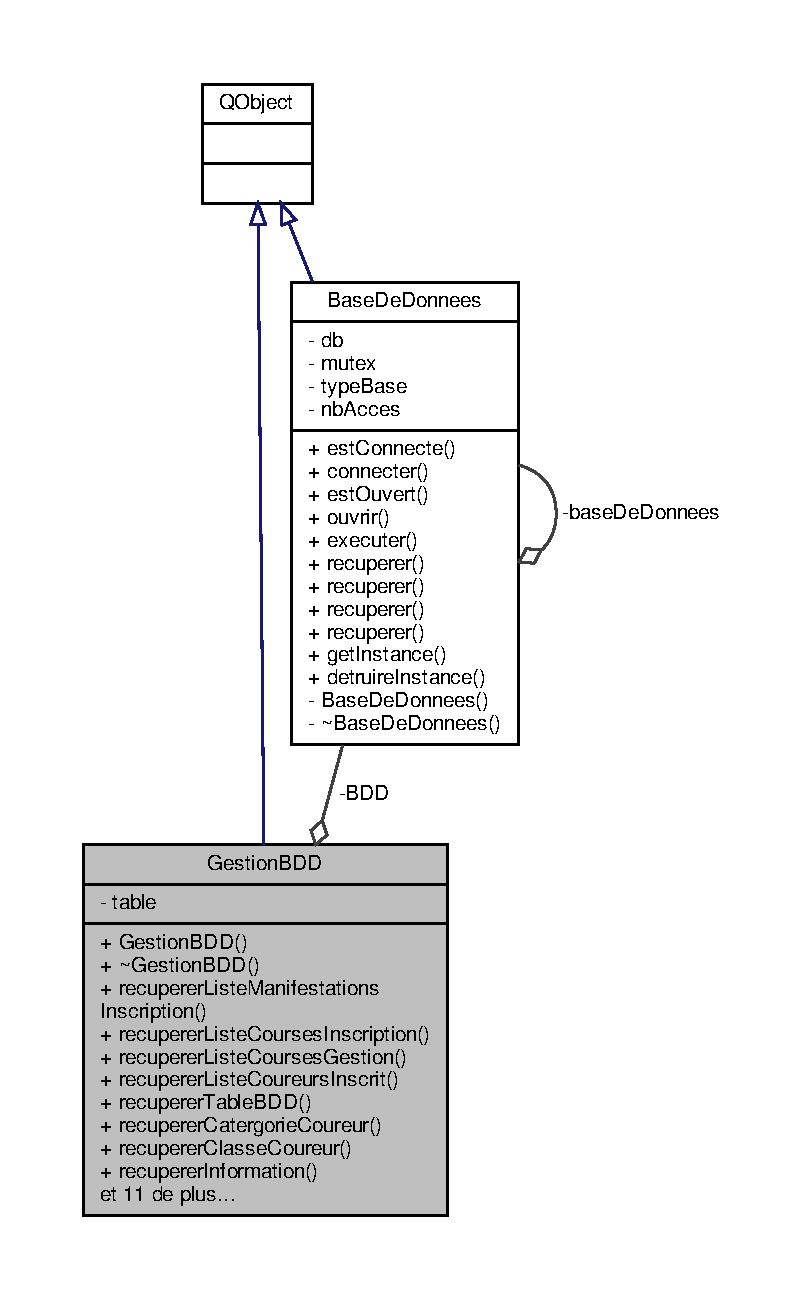
\includegraphics[height=550pt]{class_gestion_b_d_d__coll__graph}
\end{center}
\end{figure}
\subsubsection*{Signaux}
\begin{DoxyCompactItemize}
\item 
void \hyperlink{class_gestion_b_d_d_a61bc349c8942a196e2edd3083465286f}{nouvel\+Inscrit} (Q\+String\+List inscription)
\item 
void \hyperlink{class_gestion_b_d_d_acf915265e83f03b500f10ffbde2680bb}{nouveau\+Coureur} (Q\+String\+List informations\+Coureur\+Classement)
\item 
void \hyperlink{class_gestion_b_d_d_aabb5dfcdcec4ef37477fff65f6624784}{coureur\+Supprime} ()
\item 
void \hyperlink{class_gestion_b_d_d_a911c1e7a4d8bc38566512db37b13c9f0}{coureur\+Modifie} ()
\end{DoxyCompactItemize}
\subsubsection*{Fonctions membres publiques}
\begin{DoxyCompactItemize}
\item 
\hyperlink{class_gestion_b_d_d_a406bdb9b1714b204fa6fab015baffc27}{Gestion\+B\+DD} (\hyperlink{class_q_object}{Q\+Object} $\ast$parent=nullptr)
\begin{DoxyCompactList}\small\item\em Constructeur \hyperlink{class_gestion_b_d_d_a406bdb9b1714b204fa6fab015baffc27}{Gestion\+B\+D\+D()} de la classe \hyperlink{class_gestion_b_d_d}{Gestion\+B\+DD}. \end{DoxyCompactList}\item 
\hyperlink{class_gestion_b_d_d_a4d98c4008182a5749c57c97772b3c303}{$\sim$\+Gestion\+B\+DD} ()
\begin{DoxyCompactList}\small\item\em Destructeur \hyperlink{class_gestion_b_d_d_a4d98c4008182a5749c57c97772b3c303}{$\sim$\+Gestion\+B\+D\+D()} de la classe \hyperlink{class_gestion_b_d_d_a406bdb9b1714b204fa6fab015baffc27}{Gestion\+B\+D\+D()} \end{DoxyCompactList}\item 
Q\+Vector$<$ Q\+String $>$ \hyperlink{class_gestion_b_d_d_a6c1ab5e51fbd6c92bb096badbeac0df5}{recuperer\+Liste\+Manifestations\+Inscription} (Q\+String I\+NE)
\item 
Q\+Vector$<$ Q\+String $>$ \hyperlink{class_gestion_b_d_d_a59ef29e28993c64aa4d5a8c42a8fb08d}{recuperer\+Liste\+Courses\+Inscription} (Q\+String nom, Q\+String sexe)
\item 
Q\+String\+List \hyperlink{class_gestion_b_d_d_ac35de40fd5860b3130f71788ecaa5ef3}{recuperer\+Liste\+Courses\+Gestion} (Q\+String I\+NE)
\item 
Q\+Vector$<$ Q\+String\+List $>$ \hyperlink{class_gestion_b_d_d_a09b547cb065256acd269c64e273c93fd}{recuperer\+Liste\+Coureurs\+Inscrit} (Q\+String nom\+Course)
\item 
Q\+Vector$<$ Q\+String\+List $>$ \hyperlink{class_gestion_b_d_d_a2b44ebc5bf5b1a7babde6512817a85b4}{recuperer\+Table\+B\+DD} (Q\+String \hyperlink{class_gestion_b_d_d_afa3e974fb5afa7f25f275a662e182960}{table})
\item 
Q\+String \hyperlink{class_gestion_b_d_d_ad7b0117ad5d55f21e6f00858038f4a85}{recuperer\+Catergorie\+Coureur} (Q\+String id\+Categorie)
\item 
Q\+String \hyperlink{class_gestion_b_d_d_a0e90b16b2e330de9cc80f72f0d648e5d}{recuperer\+Classe\+Coureur} (Q\+String id\+Classe)
\item 
Q\+String \hyperlink{class_gestion_b_d_d_a0a2fa02b90974684658937fbfb55bf0a}{recuperer\+Information} (Q\+String info, Q\+String nom\+Table, Q\+String nom\+Enregistrement)
\item 
Q\+Vector$<$ Q\+String $>$ \hyperlink{class_gestion_b_d_d_a76ab3e307ad9005dcdb2781fc77fc5c8}{recuperer\+Categories\+Creation} ()
\item 
Q\+Vector$<$ Q\+String $>$ \hyperlink{class_gestion_b_d_d_a38d728d644f23048f1a6d3e6d4656764}{recuperer\+Classes\+Creation} ()
\item 
bool \hyperlink{class_gestion_b_d_d_af6a83eb058d71d9c583c403bf5a8ce3b}{verifier\+Creation} (Q\+String\+List enregistrement)
\item 
bool \hyperlink{class_gestion_b_d_d_abfd3cfb9553a83aafd86c3149869d6c0}{verifier\+Information} (Q\+String information, Q\+String \hyperlink{class_gestion_b_d_d_afa3e974fb5afa7f25f275a662e182960}{table})
\item 
void \hyperlink{class_gestion_b_d_d_ae71561eea6d1163ff067f079ccc6d169}{ajouter\+Nouveau\+Coureur} (Q\+String\+List enregistrement)
\item 
bool \hyperlink{class_gestion_b_d_d_a5ea332563e5be2116084ed2886c355c8}{verifier\+Modification} (Q\+String\+List enregistrement)
\item 
void \hyperlink{class_gestion_b_d_d_af64457de89c484bf854db0910bef790e}{modifier\+Enregistrement} (Q\+String\+List enregistrement)
\item 
bool \hyperlink{class_gestion_b_d_d_a1a39bbc7bfcb60d286363b9d2dd7f88b}{verifier\+Dossard} (Q\+String dossard)
\item 
void \hyperlink{class_gestion_b_d_d_a71391d5419969b52cd999463b5326599}{ajouter\+Nouvel\+Inscrit} (Q\+String\+List inscription)
\item 
void \hyperlink{class_gestion_b_d_d_afe47ec92274b7998131c5d4e6551d177}{supprimer\+Coureur} (Q\+String I\+NE)
\item 
void \hyperlink{class_gestion_b_d_d_afad096d7e405d35a818d4858ee34df61}{modifier\+Coureur} (Q\+String\+List enregistrement)
\end{DoxyCompactItemize}
\subsubsection*{Attributs privés}
\begin{DoxyCompactItemize}
\item 
\hyperlink{class_base_de_donnees}{Base\+De\+Donnees} $\ast$ \hyperlink{class_gestion_b_d_d_a1bd17cbf5754eb6e54ae351f1d02dca2}{B\+DD}
\item 
Q\+Vector$<$ Q\+String\+List $>$ \hyperlink{class_gestion_b_d_d_afa3e974fb5afa7f25f275a662e182960}{table}
\end{DoxyCompactItemize}


\subsubsection{Description détaillée}
Déclaration de la classe \hyperlink{class_gestion_b_d_d}{Gestion\+B\+DD}. 

\begin{DoxyAuthor}{Auteur}
A\+N\+D\+R\+Eo Michaël 
\end{DoxyAuthor}
\begin{DoxyVersion}{Version}
1.\+0 
\end{DoxyVersion}


\subsubsection{Documentation des constructeurs et destructeur}
\mbox{\Hypertarget{class_gestion_b_d_d_a406bdb9b1714b204fa6fab015baffc27}\label{class_gestion_b_d_d_a406bdb9b1714b204fa6fab015baffc27}} 
\index{Gestion\+B\+DD@{Gestion\+B\+DD}!Gestion\+B\+DD@{Gestion\+B\+DD}}
\index{Gestion\+B\+DD@{Gestion\+B\+DD}!Gestion\+B\+DD@{Gestion\+B\+DD}}
\paragraph{\texorpdfstring{Gestion\+B\+D\+D()}{GestionBDD()}}
{\footnotesize\ttfamily Gestion\+B\+D\+D\+::\+Gestion\+B\+DD (\begin{DoxyParamCaption}\item[{\hyperlink{class_q_object}{Q\+Object} $\ast$}]{parent = {\ttfamily nullptr} }\end{DoxyParamCaption})}



Constructeur \hyperlink{class_gestion_b_d_d_a406bdb9b1714b204fa6fab015baffc27}{Gestion\+B\+D\+D()} de la classe \hyperlink{class_gestion_b_d_d}{Gestion\+B\+DD}. 


\begin{DoxyParams}{Paramètres}
{\em parent} & \\
\hline
\end{DoxyParams}


Références \hyperlink{class_gestion_b_d_d_a1bd17cbf5754eb6e54ae351f1d02dca2}{B\+DD}, \hyperlink{class_base_de_donnees_ab2e092285ccc0ee1cce61a1774218561}{Base\+De\+Donnees\+::connecter()}, \hyperlink{class_base_de_donnees_a00388973f3ec42e5c8e76e7af7e124b2}{Base\+De\+Donnees\+::est\+Connecte()}, et \hyperlink{class_base_de_donnees_a80028aa2b6b4fbf30fb2e36357b7d3d3}{Base\+De\+Donnees\+::get\+Instance()}.


\begin{DoxyCode}
00015                                       : \hyperlink{class_q_object}{QObject}(parent)
00016 \{
00017     \hyperlink{class_gestion_b_d_d_a1bd17cbf5754eb6e54ae351f1d02dca2}{BDD} = \hyperlink{class_base_de_donnees_a80028aa2b6b4fbf30fb2e36357b7d3d3}{BaseDeDonnees::getInstance}();
00018     \textcolor{keywordflow}{if}(!\hyperlink{class_gestion_b_d_d_a1bd17cbf5754eb6e54ae351f1d02dca2}{BDD}->\hyperlink{class_base_de_donnees_a00388973f3ec42e5c8e76e7af7e124b2}{estConnecte}())
00019         \hyperlink{class_gestion_b_d_d_a1bd17cbf5754eb6e54ae351f1d02dca2}{BDD}->\hyperlink{class_base_de_donnees_ab2e092285ccc0ee1cce61a1774218561}{connecter}(\textcolor{stringliteral}{"Chrono-Cross"});
00020 
00021     qDebug() << Q\_FUNC\_INFO << \textcolor{stringliteral}{"Etat connexion BDD : "} << \hyperlink{class_gestion_b_d_d_a1bd17cbf5754eb6e54ae351f1d02dca2}{BDD}->\hyperlink{class_base_de_donnees_a00388973f3ec42e5c8e76e7af7e124b2}{estConnecte}();
00022 \}
\end{DoxyCode}
\mbox{\Hypertarget{class_gestion_b_d_d_a4d98c4008182a5749c57c97772b3c303}\label{class_gestion_b_d_d_a4d98c4008182a5749c57c97772b3c303}} 
\index{Gestion\+B\+DD@{Gestion\+B\+DD}!````~Gestion\+B\+DD@{$\sim$\+Gestion\+B\+DD}}
\index{````~Gestion\+B\+DD@{$\sim$\+Gestion\+B\+DD}!Gestion\+B\+DD@{Gestion\+B\+DD}}
\paragraph{\texorpdfstring{$\sim$\+Gestion\+B\+D\+D()}{~GestionBDD()}}
{\footnotesize\ttfamily Gestion\+B\+D\+D\+::$\sim$\+Gestion\+B\+DD (\begin{DoxyParamCaption}{ }\end{DoxyParamCaption})}



Destructeur \hyperlink{class_gestion_b_d_d_a4d98c4008182a5749c57c97772b3c303}{$\sim$\+Gestion\+B\+D\+D()} de la classe \hyperlink{class_gestion_b_d_d_a406bdb9b1714b204fa6fab015baffc27}{Gestion\+B\+D\+D()} 



Références \hyperlink{class_base_de_donnees_a457401c0816b888c77ce915997545f4e}{Base\+De\+Donnees\+::detruire\+Instance()}.


\begin{DoxyCode}
00029 \{
00030     \hyperlink{class_base_de_donnees_a457401c0816b888c77ce915997545f4e}{BaseDeDonnees::detruireInstance}();
00031     qDebug() << Q\_FUNC\_INFO;
00032 \}
\end{DoxyCode}


\subsubsection{Documentation des fonctions membres}
\mbox{\Hypertarget{class_gestion_b_d_d_ae71561eea6d1163ff067f079ccc6d169}\label{class_gestion_b_d_d_ae71561eea6d1163ff067f079ccc6d169}} 
\index{Gestion\+B\+DD@{Gestion\+B\+DD}!ajouter\+Nouveau\+Coureur@{ajouter\+Nouveau\+Coureur}}
\index{ajouter\+Nouveau\+Coureur@{ajouter\+Nouveau\+Coureur}!Gestion\+B\+DD@{Gestion\+B\+DD}}
\paragraph{\texorpdfstring{ajouter\+Nouveau\+Coureur()}{ajouterNouveauCoureur()}}
{\footnotesize\ttfamily void Gestion\+B\+D\+D\+::ajouter\+Nouveau\+Coureur (\begin{DoxyParamCaption}\item[{Q\+String\+List}]{enregistrement }\end{DoxyParamCaption})}



Références \hyperlink{class_gestion_b_d_d_a1bd17cbf5754eb6e54ae351f1d02dca2}{B\+DD}, \hyperlink{class_base_de_donnees_aa8de5f8f8bb17edc43f5c0ee33712081}{Base\+De\+Donnees\+::executer()}, \hyperlink{class_gestion_b_d_d_acf915265e83f03b500f10ffbde2680bb}{nouveau\+Coureur()}, et \hyperlink{class_base_de_donnees_a77539baad389f5acf754cd2cd452403e}{Base\+De\+Donnees\+::recuperer()}.



Référencé par \hyperlink{class_i_h_m_gestion_cross_a6000b152ba3febb45d6c409519168ba2}{I\+H\+M\+Gestion\+Cross\+::creer\+Coureur()}.


\begin{DoxyCode}
00219 \{
00220     qDebug() << informationsCoureur;
00221     QStringList informationsCoureurClassement = informationsCoureur;
00222     \textcolor{comment}{// informationsCoureur [ 0 Categorie , 1 classe , 2 INE , 3 nom ,  4 prenom , 5 dateNaissance , 6 sexe
       ]}
00223     qDebug() << Q\_FUNC\_INFO << QString(\textcolor{stringliteral}{"SELECT idCategorie FROM Categorie WHERE Nom = '%1' AND Sexe = '%2';
      "}).arg(informationsCoureur[0]).arg(informationsCoureur[6]);
00224 
00225     \textcolor{keywordtype}{bool} etat = \hyperlink{class_gestion_b_d_d_a1bd17cbf5754eb6e54ae351f1d02dca2}{BDD}->\hyperlink{class_base_de_donnees_a77539baad389f5acf754cd2cd452403e}{recuperer}(QString(\textcolor{stringliteral}{"SELECT idCategorie FROM Categorie WHERE Nom = '%1' AND
       Sexe = '%2';"}).arg(informationsCoureur[0]).arg(informationsCoureur[6]), informationsCoureur[0]);
00226 
00227     \textcolor{keywordflow}{if}(etat)
00228     \{
00229         qDebug() << Q\_FUNC\_INFO << QString(\textcolor{stringliteral}{"SELECT idCLasse FROM Classe WHERE Nom = '%1';"}).arg(
      informationsCoureur[1]);
00230 
00231         etat = \hyperlink{class_gestion_b_d_d_a1bd17cbf5754eb6e54ae351f1d02dca2}{BDD}->\hyperlink{class_base_de_donnees_a77539baad389f5acf754cd2cd452403e}{recuperer}(QString(\textcolor{stringliteral}{"SELECT idCLasse FROM Classe WHERE Nom = '%1';"}).arg(
      informationsCoureur[1]),informationsCoureur[1]);
00232         \textcolor{keywordflow}{if}(etat)
00233         \{
00234             qDebug() << Q\_FUNC\_INFO << QString(\textcolor{stringliteral}{"INSERT INTO `Coureur`(`idCoureur`, `idCategorie`,
       `idClasse`, `INE`, `Nom`, `Prenom`, `DateNaissance`, `Sexe`) VALUES (`idCoureur`,%0,%1,'%2','%3','%4','%5','%6')"}).
      arg(informationsCoureur[0]).arg(informationsCoureur[1]).arg(informationsCoureur[2]).arg(informationsCoureur[3]
      ).arg(informationsCoureur[4]).arg(informationsCoureur[5]).arg(informationsCoureur[6]);
00235 
00236             etat = \hyperlink{class_gestion_b_d_d_a1bd17cbf5754eb6e54ae351f1d02dca2}{BDD}->\hyperlink{class_base_de_donnees_aa8de5f8f8bb17edc43f5c0ee33712081}{executer}(QString(\textcolor{stringliteral}{"INSERT INTO `Coureur`(`idCoureur`, `idCategorie`,
       `idClasse`, `INE`, `Nom`, `Prenom`, `DateNaissance`, `Sexe`) VALUES (`idCoureur`,%0,%1,'%2','%3','%4','%5','%6')
      "}).arg(informationsCoureur[0]).arg(informationsCoureur[1]).arg(informationsCoureur[2]).arg(
      informationsCoureur[3]).arg(informationsCoureur[4]).arg(informationsCoureur[5]).arg(informationsCoureur[6]));
00237             \textcolor{keywordflow}{if}(etat)
00238             \{
00239                 qDebug() << Q\_FUNC\_INFO << \textcolor{stringliteral}{"Enregistré(e) avec Succées !"};
00240                 emit \hyperlink{class_gestion_b_d_d_acf915265e83f03b500f10ffbde2680bb}{nouveauCoureur}(informationsCoureurClassement);
00241             \}
00242         \}
00243         \textcolor{keywordflow}{else}
00244         \{
00245             qDebug() << Q\_FUNC\_INFO << \textcolor{stringliteral}{"ERREUR"};
00246             informationsCoureurClassement.clear();
00247         \}
00248     \}
00249     \textcolor{keywordflow}{else}
00250     \{
00251         qDebug() << Q\_FUNC\_INFO << \textcolor{stringliteral}{"ERREUR"};
00252         informationsCoureurClassement.clear();
00253     \}
00254 \}
\end{DoxyCode}
\mbox{\Hypertarget{class_gestion_b_d_d_a71391d5419969b52cd999463b5326599}\label{class_gestion_b_d_d_a71391d5419969b52cd999463b5326599}} 
\index{Gestion\+B\+DD@{Gestion\+B\+DD}!ajouter\+Nouvel\+Inscrit@{ajouter\+Nouvel\+Inscrit}}
\index{ajouter\+Nouvel\+Inscrit@{ajouter\+Nouvel\+Inscrit}!Gestion\+B\+DD@{Gestion\+B\+DD}}
\paragraph{\texorpdfstring{ajouter\+Nouvel\+Inscrit()}{ajouterNouvelInscrit()}}
{\footnotesize\ttfamily void Gestion\+B\+D\+D\+::ajouter\+Nouvel\+Inscrit (\begin{DoxyParamCaption}\item[{Q\+String\+List}]{inscription }\end{DoxyParamCaption})}



Références \hyperlink{class_gestion_b_d_d_a1bd17cbf5754eb6e54ae351f1d02dca2}{B\+DD}, \hyperlink{class_base_de_donnees_aa8de5f8f8bb17edc43f5c0ee33712081}{Base\+De\+Donnees\+::executer()}, \hyperlink{class_gestion_b_d_d_a61bc349c8942a196e2edd3083465286f}{nouvel\+Inscrit()}, et \hyperlink{class_base_de_donnees_a77539baad389f5acf754cd2cd452403e}{Base\+De\+Donnees\+::recuperer()}.



Référencé par \hyperlink{class_i_h_m_gestion_cross_af0165d32344af78b4edce59f88c90ff6}{I\+H\+M\+Gestion\+Cross\+::ajouter\+Nouvelle\+Inscription()}.


\begin{DoxyCode}
00257 \{
00258     \textcolor{comment}{// inscription [ idCoureur , idCourse , numeroDossard ]}
00259     qDebug() << Q\_FUNC\_INFO << inscription;
00260     \textcolor{keywordtype}{bool} etat = \hyperlink{class_gestion_b_d_d_a1bd17cbf5754eb6e54ae351f1d02dca2}{BDD}->\hyperlink{class_base_de_donnees_aa8de5f8f8bb17edc43f5c0ee33712081}{executer}(QString(\textcolor{stringliteral}{"INSERT INTO `Inscrit`(`idInscrit`, `idCoureur`,
       `idCourse`, `NumeroDossard`) VALUES (`idInscrit`,'%1','%2','%3')"}).arg(inscription[0]).arg(inscription[1]).arg(
      inscription[2]));
00261     qDebug() << Q\_FUNC\_INFO << \textcolor{stringliteral}{"Ajout : "} << etat;
00262     \textcolor{keywordflow}{if}(etat)
00263     \{
00264         QString idCoureur = inscription[0];
00265         QString dossard = inscription[2];
00266         inscription.clear();
00267         etat = \hyperlink{class_gestion_b_d_d_a1bd17cbf5754eb6e54ae351f1d02dca2}{BDD}->\hyperlink{class_base_de_donnees_a77539baad389f5acf754cd2cd452403e}{recuperer}(QString(\textcolor{stringliteral}{"SELECT Nom, Prenom FROM Coureur WHERE idCoureur = '%1';"}
      ).arg(idCoureur), inscription);
00268         inscription << dossard;
00269         qDebug() << Q\_FUNC\_INFO << inscription;
00270         emit \hyperlink{class_gestion_b_d_d_a61bc349c8942a196e2edd3083465286f}{nouvelInscrit}(inscription);
00271     \}
00272 \}
\end{DoxyCode}
\mbox{\Hypertarget{class_gestion_b_d_d_a911c1e7a4d8bc38566512db37b13c9f0}\label{class_gestion_b_d_d_a911c1e7a4d8bc38566512db37b13c9f0}} 
\index{Gestion\+B\+DD@{Gestion\+B\+DD}!coureur\+Modifie@{coureur\+Modifie}}
\index{coureur\+Modifie@{coureur\+Modifie}!Gestion\+B\+DD@{Gestion\+B\+DD}}
\paragraph{\texorpdfstring{coureur\+Modifie}{coureurModifie}}
{\footnotesize\ttfamily void Gestion\+B\+D\+D\+::coureur\+Modifie (\begin{DoxyParamCaption}{ }\end{DoxyParamCaption})\hspace{0.3cm}{\ttfamily [signal]}}



Référencé par \hyperlink{class_gestion_b_d_d_afad096d7e405d35a818d4858ee34df61}{modifier\+Coureur()}.

\mbox{\Hypertarget{class_gestion_b_d_d_aabb5dfcdcec4ef37477fff65f6624784}\label{class_gestion_b_d_d_aabb5dfcdcec4ef37477fff65f6624784}} 
\index{Gestion\+B\+DD@{Gestion\+B\+DD}!coureur\+Supprime@{coureur\+Supprime}}
\index{coureur\+Supprime@{coureur\+Supprime}!Gestion\+B\+DD@{Gestion\+B\+DD}}
\paragraph{\texorpdfstring{coureur\+Supprime}{coureurSupprime}}
{\footnotesize\ttfamily void Gestion\+B\+D\+D\+::coureur\+Supprime (\begin{DoxyParamCaption}{ }\end{DoxyParamCaption})\hspace{0.3cm}{\ttfamily [signal]}}



Référencé par \hyperlink{class_gestion_b_d_d_afe47ec92274b7998131c5d4e6551d177}{supprimer\+Coureur()}.

\mbox{\Hypertarget{class_gestion_b_d_d_afad096d7e405d35a818d4858ee34df61}\label{class_gestion_b_d_d_afad096d7e405d35a818d4858ee34df61}} 
\index{Gestion\+B\+DD@{Gestion\+B\+DD}!modifier\+Coureur@{modifier\+Coureur}}
\index{modifier\+Coureur@{modifier\+Coureur}!Gestion\+B\+DD@{Gestion\+B\+DD}}
\paragraph{\texorpdfstring{modifier\+Coureur()}{modifierCoureur()}}
{\footnotesize\ttfamily void Gestion\+B\+D\+D\+::modifier\+Coureur (\begin{DoxyParamCaption}\item[{Q\+String\+List}]{enregistrement }\end{DoxyParamCaption})}



Références \hyperlink{class_gestion_b_d_d_a1bd17cbf5754eb6e54ae351f1d02dca2}{B\+DD}, \hyperlink{class_gestion_b_d_d_a911c1e7a4d8bc38566512db37b13c9f0}{coureur\+Modifie()}, \hyperlink{class_base_de_donnees_aa8de5f8f8bb17edc43f5c0ee33712081}{Base\+De\+Donnees\+::executer()}, et \hyperlink{class_base_de_donnees_a77539baad389f5acf754cd2cd452403e}{Base\+De\+Donnees\+::recuperer()}.



Référencé par \hyperlink{class_i_h_m_gestion_cross_a144933ab31ae263be7267b93bfd53a82}{I\+H\+M\+Gestion\+Cross\+::confirmer\+Dialog()}.


\begin{DoxyCode}
00293 \{
00294     \textcolor{comment}{// enregistrement [ 0 Categorie , 1 classe , 2 INE , 3 nom , 4 prenom , 5 dateNaissance , 6 sexe  , 7
       idCoureur]}
00295 
00296     qDebug() << Q\_FUNC\_INFO << enregistrement;
00297     \textcolor{keywordtype}{bool} etat = \hyperlink{class_gestion_b_d_d_a1bd17cbf5754eb6e54ae351f1d02dca2}{BDD}->\hyperlink{class_base_de_donnees_a77539baad389f5acf754cd2cd452403e}{recuperer}(QString(\textcolor{stringliteral}{"SELECT idCategorie FROM Categorie WHERE Nom = '%1';"}).
      arg(enregistrement[0]), enregistrement[0]);
00298     etat = \hyperlink{class_gestion_b_d_d_a1bd17cbf5754eb6e54ae351f1d02dca2}{BDD}->\hyperlink{class_base_de_donnees_a77539baad389f5acf754cd2cd452403e}{recuperer}(QString(\textcolor{stringliteral}{"SELECT idClasse FROM Classe WHERE Nom = '%1';"}).arg(
      enregistrement[1]), enregistrement[1]);
00299 
00300     etat = \hyperlink{class_gestion_b_d_d_a1bd17cbf5754eb6e54ae351f1d02dca2}{BDD}->\hyperlink{class_base_de_donnees_aa8de5f8f8bb17edc43f5c0ee33712081}{executer}(QString(\textcolor{stringliteral}{"UPDATE `Coureur` SET
       `idCategorie`='%1',`idClasse`='%2',`INE`='%3',`Nom`='%4',`Prenom`='%5',`DateNaissance`='%6',`Sexe`='%7' WHERE idCoureur = '%8';"}).arg(enregistrement[
      0]).arg(enregistrement[1]).arg(enregistrement[2]).arg(enregistrement[3]).arg(enregistrement[4]).arg(
      enregistrement[5]).arg(enregistrement[6]).arg(enregistrement[7]));
00301     qDebug() << Q\_FUNC\_INFO << \textcolor{stringliteral}{"Modification : "} << etat;
00302     \textcolor{keywordflow}{if}(etat)
00303         emit \hyperlink{class_gestion_b_d_d_a911c1e7a4d8bc38566512db37b13c9f0}{coureurModifie}();
00304 \}
\end{DoxyCode}
\mbox{\Hypertarget{class_gestion_b_d_d_af64457de89c484bf854db0910bef790e}\label{class_gestion_b_d_d_af64457de89c484bf854db0910bef790e}} 
\index{Gestion\+B\+DD@{Gestion\+B\+DD}!modifier\+Enregistrement@{modifier\+Enregistrement}}
\index{modifier\+Enregistrement@{modifier\+Enregistrement}!Gestion\+B\+DD@{Gestion\+B\+DD}}
\paragraph{\texorpdfstring{modifier\+Enregistrement()}{modifierEnregistrement()}}
{\footnotesize\ttfamily void Gestion\+B\+D\+D\+::modifier\+Enregistrement (\begin{DoxyParamCaption}\item[{Q\+String\+List}]{enregistrement }\end{DoxyParamCaption})}

\mbox{\Hypertarget{class_gestion_b_d_d_acf915265e83f03b500f10ffbde2680bb}\label{class_gestion_b_d_d_acf915265e83f03b500f10ffbde2680bb}} 
\index{Gestion\+B\+DD@{Gestion\+B\+DD}!nouveau\+Coureur@{nouveau\+Coureur}}
\index{nouveau\+Coureur@{nouveau\+Coureur}!Gestion\+B\+DD@{Gestion\+B\+DD}}
\paragraph{\texorpdfstring{nouveau\+Coureur}{nouveauCoureur}}
{\footnotesize\ttfamily void Gestion\+B\+D\+D\+::nouveau\+Coureur (\begin{DoxyParamCaption}\item[{Q\+String\+List}]{informations\+Coureur\+Classement }\end{DoxyParamCaption})\hspace{0.3cm}{\ttfamily [signal]}}



Référencé par \hyperlink{class_gestion_b_d_d_ae71561eea6d1163ff067f079ccc6d169}{ajouter\+Nouveau\+Coureur()}.

\mbox{\Hypertarget{class_gestion_b_d_d_a61bc349c8942a196e2edd3083465286f}\label{class_gestion_b_d_d_a61bc349c8942a196e2edd3083465286f}} 
\index{Gestion\+B\+DD@{Gestion\+B\+DD}!nouvel\+Inscrit@{nouvel\+Inscrit}}
\index{nouvel\+Inscrit@{nouvel\+Inscrit}!Gestion\+B\+DD@{Gestion\+B\+DD}}
\paragraph{\texorpdfstring{nouvel\+Inscrit}{nouvelInscrit}}
{\footnotesize\ttfamily void Gestion\+B\+D\+D\+::nouvel\+Inscrit (\begin{DoxyParamCaption}\item[{Q\+String\+List}]{inscription }\end{DoxyParamCaption})\hspace{0.3cm}{\ttfamily [signal]}}



Référencé par \hyperlink{class_gestion_b_d_d_a71391d5419969b52cd999463b5326599}{ajouter\+Nouvel\+Inscrit()}.

\mbox{\Hypertarget{class_gestion_b_d_d_a76ab3e307ad9005dcdb2781fc77fc5c8}\label{class_gestion_b_d_d_a76ab3e307ad9005dcdb2781fc77fc5c8}} 
\index{Gestion\+B\+DD@{Gestion\+B\+DD}!recuperer\+Categories\+Creation@{recuperer\+Categories\+Creation}}
\index{recuperer\+Categories\+Creation@{recuperer\+Categories\+Creation}!Gestion\+B\+DD@{Gestion\+B\+DD}}
\paragraph{\texorpdfstring{recuperer\+Categories\+Creation()}{recupererCategoriesCreation()}}
{\footnotesize\ttfamily Q\+Vector$<$ Q\+String $>$ Gestion\+B\+D\+D\+::recuperer\+Categories\+Creation (\begin{DoxyParamCaption}{ }\end{DoxyParamCaption})}



Références \hyperlink{class_gestion_b_d_d_a1bd17cbf5754eb6e54ae351f1d02dca2}{B\+DD}, et \hyperlink{class_base_de_donnees_a77539baad389f5acf754cd2cd452403e}{Base\+De\+Donnees\+::recuperer()}.



Référencé par \hyperlink{class_i_h_m_gestion_cross_ac8f336c95a5f0c9eb8a4bc1c4bb83445}{I\+H\+M\+Gestion\+Cross\+::passer\+Mode\+Nouveau\+Coureur()}.


\begin{DoxyCode}
00171 \{
00172     QVector<QString> categories;
00173     \textcolor{keywordtype}{bool} etat = \hyperlink{class_gestion_b_d_d_a1bd17cbf5754eb6e54ae351f1d02dca2}{BDD}->\hyperlink{class_base_de_donnees_a77539baad389f5acf754cd2cd452403e}{recuperer}(\textcolor{stringliteral}{"SELECT DISTINCT Nom FROM Categorie WHERE 1;"}, categories);
00174     \textcolor{keywordflow}{if}(etat)
00175     \{
00176         \textcolor{keywordflow}{return} categories;
00177     \}
00178     \textcolor{keywordflow}{else}
00179     \{
00180         qDebug() << Q\_FUNC\_INFO << \textcolor{stringliteral}{"ERREUR"};
00181         \textcolor{keywordflow}{return} categories;
00182     \}
00183 \}
\end{DoxyCode}
\mbox{\Hypertarget{class_gestion_b_d_d_ad7b0117ad5d55f21e6f00858038f4a85}\label{class_gestion_b_d_d_ad7b0117ad5d55f21e6f00858038f4a85}} 
\index{Gestion\+B\+DD@{Gestion\+B\+DD}!recuperer\+Catergorie\+Coureur@{recuperer\+Catergorie\+Coureur}}
\index{recuperer\+Catergorie\+Coureur@{recuperer\+Catergorie\+Coureur}!Gestion\+B\+DD@{Gestion\+B\+DD}}
\paragraph{\texorpdfstring{recuperer\+Catergorie\+Coureur()}{recupererCatergorieCoureur()}}
{\footnotesize\ttfamily Q\+String Gestion\+B\+D\+D\+::recuperer\+Catergorie\+Coureur (\begin{DoxyParamCaption}\item[{Q\+String}]{id\+Categorie }\end{DoxyParamCaption})}



Références \hyperlink{class_gestion_b_d_d_a1bd17cbf5754eb6e54ae351f1d02dca2}{B\+DD}, et \hyperlink{class_base_de_donnees_a77539baad389f5acf754cd2cd452403e}{Base\+De\+Donnees\+::recuperer()}.


\begin{DoxyCode}
00133 \{
00134     QString id;
00135     \textcolor{keywordtype}{bool} etat = \hyperlink{class_gestion_b_d_d_a1bd17cbf5754eb6e54ae351f1d02dca2}{BDD}->\hyperlink{class_base_de_donnees_a77539baad389f5acf754cd2cd452403e}{recuperer}(QString(\textcolor{stringliteral}{"SELECT Nom FROM Categorie WHERE idCategorie = %1;"}).arg
      (idCategorie), \textcolor{keywordtype}{id});
00136     \textcolor{keywordflow}{if}(etat)
00137         \textcolor{keywordflow}{return} id;
00138     \textcolor{keywordflow}{else}
00139     \{
00140         qDebug() << Q\_FUNC\_INFO << \textcolor{stringliteral}{"ERREUR"};
00141         \textcolor{keywordflow}{return} id;
00142     \}
00143 \}
\end{DoxyCode}
\mbox{\Hypertarget{class_gestion_b_d_d_a0e90b16b2e330de9cc80f72f0d648e5d}\label{class_gestion_b_d_d_a0e90b16b2e330de9cc80f72f0d648e5d}} 
\index{Gestion\+B\+DD@{Gestion\+B\+DD}!recuperer\+Classe\+Coureur@{recuperer\+Classe\+Coureur}}
\index{recuperer\+Classe\+Coureur@{recuperer\+Classe\+Coureur}!Gestion\+B\+DD@{Gestion\+B\+DD}}
\paragraph{\texorpdfstring{recuperer\+Classe\+Coureur()}{recupererClasseCoureur()}}
{\footnotesize\ttfamily Q\+String Gestion\+B\+D\+D\+::recuperer\+Classe\+Coureur (\begin{DoxyParamCaption}\item[{Q\+String}]{id\+Classe }\end{DoxyParamCaption})}



Références \hyperlink{class_gestion_b_d_d_a1bd17cbf5754eb6e54ae351f1d02dca2}{B\+DD}, et \hyperlink{class_base_de_donnees_a77539baad389f5acf754cd2cd452403e}{Base\+De\+Donnees\+::recuperer()}.


\begin{DoxyCode}
00146 \{
00147     QString id;
00148     \textcolor{keywordtype}{bool} etat = \hyperlink{class_gestion_b_d_d_a1bd17cbf5754eb6e54ae351f1d02dca2}{BDD}->\hyperlink{class_base_de_donnees_a77539baad389f5acf754cd2cd452403e}{recuperer}(QString(\textcolor{stringliteral}{"SELECT Nom FROM Classe WHERE idClasse = %1;"}).arg(
      idClasse), \textcolor{keywordtype}{id});
00149     \textcolor{keywordflow}{if}(etat)
00150         \textcolor{keywordflow}{return} id;
00151     \textcolor{keywordflow}{else}
00152     \{
00153         qDebug() << Q\_FUNC\_INFO << \textcolor{stringliteral}{"ERREUR"};
00154         \textcolor{keywordflow}{return} id;
00155     \}
00156 \}
\end{DoxyCode}
\mbox{\Hypertarget{class_gestion_b_d_d_a38d728d644f23048f1a6d3e6d4656764}\label{class_gestion_b_d_d_a38d728d644f23048f1a6d3e6d4656764}} 
\index{Gestion\+B\+DD@{Gestion\+B\+DD}!recuperer\+Classes\+Creation@{recuperer\+Classes\+Creation}}
\index{recuperer\+Classes\+Creation@{recuperer\+Classes\+Creation}!Gestion\+B\+DD@{Gestion\+B\+DD}}
\paragraph{\texorpdfstring{recuperer\+Classes\+Creation()}{recupererClassesCreation()}}
{\footnotesize\ttfamily Q\+Vector$<$ Q\+String $>$ Gestion\+B\+D\+D\+::recuperer\+Classes\+Creation (\begin{DoxyParamCaption}{ }\end{DoxyParamCaption})}



Références \hyperlink{class_gestion_b_d_d_a1bd17cbf5754eb6e54ae351f1d02dca2}{B\+DD}, et \hyperlink{class_base_de_donnees_a77539baad389f5acf754cd2cd452403e}{Base\+De\+Donnees\+::recuperer()}.



Référencé par \hyperlink{class_i_h_m_gestion_cross_ac8f336c95a5f0c9eb8a4bc1c4bb83445}{I\+H\+M\+Gestion\+Cross\+::passer\+Mode\+Nouveau\+Coureur()}.


\begin{DoxyCode}
00186 \{
00187     QVector<QString> classes;
00188     \textcolor{keywordtype}{bool} etat = \hyperlink{class_gestion_b_d_d_a1bd17cbf5754eb6e54ae351f1d02dca2}{BDD}->\hyperlink{class_base_de_donnees_a77539baad389f5acf754cd2cd452403e}{recuperer}(\textcolor{stringliteral}{"SELECT DISTINCT Nom FROM Classe;"}, classes);
00189     \textcolor{keywordflow}{if}(etat)
00190     \{
00191         \textcolor{keywordflow}{return} classes;
00192     \}
00193     \textcolor{keywordflow}{else}
00194     \{
00195         qDebug() << Q\_FUNC\_INFO << \textcolor{stringliteral}{"ERREUR"};
00196         \textcolor{keywordflow}{return} classes;
00197     \}
00198 \}
\end{DoxyCode}
\mbox{\Hypertarget{class_gestion_b_d_d_a0a2fa02b90974684658937fbfb55bf0a}\label{class_gestion_b_d_d_a0a2fa02b90974684658937fbfb55bf0a}} 
\index{Gestion\+B\+DD@{Gestion\+B\+DD}!recuperer\+Information@{recuperer\+Information}}
\index{recuperer\+Information@{recuperer\+Information}!Gestion\+B\+DD@{Gestion\+B\+DD}}
\paragraph{\texorpdfstring{recuperer\+Information()}{recupererInformation()}}
{\footnotesize\ttfamily Q\+String Gestion\+B\+D\+D\+::recuperer\+Information (\begin{DoxyParamCaption}\item[{Q\+String}]{info,  }\item[{Q\+String}]{nom\+Table,  }\item[{Q\+String}]{nom\+Enregistrement }\end{DoxyParamCaption})}



Références \hyperlink{class_gestion_b_d_d_a1bd17cbf5754eb6e54ae351f1d02dca2}{B\+DD}, et \hyperlink{class_base_de_donnees_a77539baad389f5acf754cd2cd452403e}{Base\+De\+Donnees\+::recuperer()}.



Référencé par \hyperlink{class_i_h_m_gestion_cross_ae1510779a1efa3defecb517467e84f91}{I\+H\+M\+Gestion\+Cross\+::afficher\+Table()}, \hyperlink{class_i_h_m_gestion_cross_af0165d32344af78b4edce59f88c90ff6}{I\+H\+M\+Gestion\+Cross\+::ajouter\+Nouvelle\+Inscription()}, \hyperlink{class_i_h_m_gestion_cross_ad71963d500fd61995fdae94e833db163}{I\+H\+M\+Gestion\+Cross\+::selectionner\+Coureur()}, \hyperlink{class_i_h_m_gestion_cross_ae555b32462455a2cdaf0f8dc2e016d14}{I\+H\+M\+Gestion\+Cross\+::selectionner\+Course()}, et \hyperlink{class_i_h_m_gestion_cross_a164be2d046cf18ee03e3939d03a5580d}{I\+H\+M\+Gestion\+Cross\+::verifier\+Numero\+Dossard\+Inscription()}.


\begin{DoxyCode}
00159 \{
00160     \textcolor{keywordtype}{bool} etat = \hyperlink{class_gestion_b_d_d_a1bd17cbf5754eb6e54ae351f1d02dca2}{BDD}->\hyperlink{class_base_de_donnees_a77539baad389f5acf754cd2cd452403e}{recuperer}(QString(\textcolor{stringliteral}{"SELECT %1 FROM %2 WHERE %3;"}).arg(information).arg(
      nomTable).arg(nomEnregistrement), information);
00161     \textcolor{keywordflow}{if}(etat)
00162         \textcolor{keywordflow}{return} information;
00163     \textcolor{keywordflow}{else}
00164     \{
00165         qDebug() << Q\_FUNC\_INFO << \textcolor{stringliteral}{"ERREUR"};
00166         \textcolor{keywordflow}{return} information;
00167     \}
00168 \}
\end{DoxyCode}
\mbox{\Hypertarget{class_gestion_b_d_d_a09b547cb065256acd269c64e273c93fd}\label{class_gestion_b_d_d_a09b547cb065256acd269c64e273c93fd}} 
\index{Gestion\+B\+DD@{Gestion\+B\+DD}!recuperer\+Liste\+Coureurs\+Inscrit@{recuperer\+Liste\+Coureurs\+Inscrit}}
\index{recuperer\+Liste\+Coureurs\+Inscrit@{recuperer\+Liste\+Coureurs\+Inscrit}!Gestion\+B\+DD@{Gestion\+B\+DD}}
\paragraph{\texorpdfstring{recuperer\+Liste\+Coureurs\+Inscrit()}{recupererListeCoureursInscrit()}}
{\footnotesize\ttfamily Q\+Vector$<$ Q\+String\+List $>$ Gestion\+B\+D\+D\+::recuperer\+Liste\+Coureurs\+Inscrit (\begin{DoxyParamCaption}\item[{Q\+String}]{nom\+Course }\end{DoxyParamCaption})}



Références \hyperlink{class_gestion_b_d_d_a1bd17cbf5754eb6e54ae351f1d02dca2}{B\+DD}, et \hyperlink{class_base_de_donnees_a77539baad389f5acf754cd2cd452403e}{Base\+De\+Donnees\+::recuperer()}.



Référencé par \hyperlink{class_i_h_m_gestion_cross_ae555b32462455a2cdaf0f8dc2e016d14}{I\+H\+M\+Gestion\+Cross\+::selectionner\+Course()}.


\begin{DoxyCode}
00043 \{
00044     QString idCourse;
00045     \textcolor{keywordtype}{bool} etat = \hyperlink{class_gestion_b_d_d_a1bd17cbf5754eb6e54ae351f1d02dca2}{BDD}->\hyperlink{class_base_de_donnees_a77539baad389f5acf754cd2cd452403e}{recuperer}(QString(\textcolor{stringliteral}{"SELECT idCourse FROM Course WHERE Nom = '%1'"}).arg(
      nomCourse), idCourse);
00046 
00047     QVector<QStringList> liste;
00048     etat = \hyperlink{class_gestion_b_d_d_a1bd17cbf5754eb6e54ae351f1d02dca2}{BDD}->\hyperlink{class_base_de_donnees_a77539baad389f5acf754cd2cd452403e}{recuperer}(QString(\textcolor{stringliteral}{"SELECT Nom, Prenom, NumeroDossard FROM `Inscrit` JOIN
       Coureur ON Inscrit.idCoureur=Coureur.idCoureur WHERE Inscrit.idCourse=%1;"}).arg(idCourse), liste);
00049     qDebug() << Q\_FUNC\_INFO << etat;
00050     \textcolor{keywordflow}{return} liste;
00051 \}
\end{DoxyCode}
\mbox{\Hypertarget{class_gestion_b_d_d_ac35de40fd5860b3130f71788ecaa5ef3}\label{class_gestion_b_d_d_ac35de40fd5860b3130f71788ecaa5ef3}} 
\index{Gestion\+B\+DD@{Gestion\+B\+DD}!recuperer\+Liste\+Courses\+Gestion@{recuperer\+Liste\+Courses\+Gestion}}
\index{recuperer\+Liste\+Courses\+Gestion@{recuperer\+Liste\+Courses\+Gestion}!Gestion\+B\+DD@{Gestion\+B\+DD}}
\paragraph{\texorpdfstring{recuperer\+Liste\+Courses\+Gestion()}{recupererListeCoursesGestion()}}
{\footnotesize\ttfamily Q\+String\+List Gestion\+B\+D\+D\+::recuperer\+Liste\+Courses\+Gestion (\begin{DoxyParamCaption}\item[{Q\+String}]{I\+NE }\end{DoxyParamCaption})}



Références \hyperlink{class_gestion_b_d_d_a1bd17cbf5754eb6e54ae351f1d02dca2}{B\+DD}, et \hyperlink{class_base_de_donnees_a77539baad389f5acf754cd2cd452403e}{Base\+De\+Donnees\+::recuperer()}.



Référencé par \hyperlink{class_i_h_m_gestion_cross_ad71963d500fd61995fdae94e833db163}{I\+H\+M\+Gestion\+Cross\+::selectionner\+Coureur()}.


\begin{DoxyCode}
00116 \{
00117     QVector<QString> idCourses;
00118     QStringList nomCourses;
00119     \textcolor{keywordtype}{bool} etat = \hyperlink{class_gestion_b_d_d_a1bd17cbf5754eb6e54ae351f1d02dca2}{BDD}->\hyperlink{class_base_de_donnees_a77539baad389f5acf754cd2cd452403e}{recuperer}(QString(\textcolor{stringliteral}{"SELECT `Course`.idCourse FROM `Course` JOIN `Inscrit`
       ON `Course`.idCourse=`Inscrit`.idCourse JOIN `Coureur` ON `Inscrit`.idCoureur=`Coureur`.idCoureur WHERE
       INE='%1';"}).arg(INE), idCourses);
00120     \textcolor{keywordtype}{int} nbId = idCourses.size();
00121     qDebug() << Q\_FUNC\_INFO << etat << \textcolor{stringliteral}{"nbID : "} << nbId << \textcolor{stringliteral}{"IDs : "} << idCourses;
00122 
00123     \textcolor{keywordflow}{for}(\textcolor{keywordtype}{int} i = 0; i < nbId; i += 1)
00124     \{
00125         qDebug() << idCourses[i];
00126         etat = \hyperlink{class_gestion_b_d_d_a1bd17cbf5754eb6e54ae351f1d02dca2}{BDD}->\hyperlink{class_base_de_donnees_a77539baad389f5acf754cd2cd452403e}{recuperer}(QString(\textcolor{stringliteral}{"SELECT Nom FROM Course WHERE idCourse = '%1';"}).arg(
      idCourses[i]), nomCourses);
00127     \}
00128     qDebug() << Q\_FUNC\_INFO << nomCourses;
00129     \textcolor{keywordflow}{return} nomCourses;
00130 \}
\end{DoxyCode}
\mbox{\Hypertarget{class_gestion_b_d_d_a59ef29e28993c64aa4d5a8c42a8fb08d}\label{class_gestion_b_d_d_a59ef29e28993c64aa4d5a8c42a8fb08d}} 
\index{Gestion\+B\+DD@{Gestion\+B\+DD}!recuperer\+Liste\+Courses\+Inscription@{recuperer\+Liste\+Courses\+Inscription}}
\index{recuperer\+Liste\+Courses\+Inscription@{recuperer\+Liste\+Courses\+Inscription}!Gestion\+B\+DD@{Gestion\+B\+DD}}
\paragraph{\texorpdfstring{recuperer\+Liste\+Courses\+Inscription()}{recupererListeCoursesInscription()}}
{\footnotesize\ttfamily Q\+Vector$<$ Q\+String $>$ Gestion\+B\+D\+D\+::recuperer\+Liste\+Courses\+Inscription (\begin{DoxyParamCaption}\item[{Q\+String}]{nom,  }\item[{Q\+String}]{sexe }\end{DoxyParamCaption})}



Références \hyperlink{class_gestion_b_d_d_a1bd17cbf5754eb6e54ae351f1d02dca2}{B\+DD}, et \hyperlink{class_base_de_donnees_a77539baad389f5acf754cd2cd452403e}{Base\+De\+Donnees\+::recuperer()}.



Référencé par \hyperlink{class_i_h_m_gestion_cross_a34567afe3e94862ebd9af51528dedb65}{I\+H\+M\+Gestion\+Cross\+::lister\+Courses()}.


\begin{DoxyCode}
00103 \{
00104     QVector<QString> listeCourses;
00105     \textcolor{keywordtype}{bool} etat = \hyperlink{class_gestion_b_d_d_a1bd17cbf5754eb6e54ae351f1d02dca2}{BDD}->\hyperlink{class_base_de_donnees_a77539baad389f5acf754cd2cd452403e}{recuperer}(QString(\textcolor{stringliteral}{"SELECT Course.Nom FROM `Course` JOIN Manifestation ON
       Manifestation.idManifestation=Course.idManifestation WHERE Manifestation.Nom = '%1' AND Course.Nom LIKE '%%2'
       ORDER BY HeureDepart ASC;"}).arg(nom).arg(sexe), listeCourses);
00106     \textcolor{keywordflow}{if}(etat)
00107         \textcolor{keywordflow}{return} listeCourses;
00108     \textcolor{keywordflow}{else}
00109     \{
00110         qDebug() << Q\_FUNC\_INFO << \textcolor{stringliteral}{"ERREUR"};
00111         \textcolor{keywordflow}{return} listeCourses;
00112     \}
00113 \}
\end{DoxyCode}
\mbox{\Hypertarget{class_gestion_b_d_d_a6c1ab5e51fbd6c92bb096badbeac0df5}\label{class_gestion_b_d_d_a6c1ab5e51fbd6c92bb096badbeac0df5}} 
\index{Gestion\+B\+DD@{Gestion\+B\+DD}!recuperer\+Liste\+Manifestations\+Inscription@{recuperer\+Liste\+Manifestations\+Inscription}}
\index{recuperer\+Liste\+Manifestations\+Inscription@{recuperer\+Liste\+Manifestations\+Inscription}!Gestion\+B\+DD@{Gestion\+B\+DD}}
\paragraph{\texorpdfstring{recuperer\+Liste\+Manifestations\+Inscription()}{recupererListeManifestationsInscription()}}
{\footnotesize\ttfamily Q\+Vector$<$ Q\+String $>$ Gestion\+B\+D\+D\+::recuperer\+Liste\+Manifestations\+Inscription (\begin{DoxyParamCaption}\item[{Q\+String}]{I\+NE }\end{DoxyParamCaption})}



Références \hyperlink{class_gestion_b_d_d_a1bd17cbf5754eb6e54ae351f1d02dca2}{B\+DD}, et \hyperlink{class_base_de_donnees_a77539baad389f5acf754cd2cd452403e}{Base\+De\+Donnees\+::recuperer()}.



Référencé par \hyperlink{class_i_h_m_gestion_cross_a0eadd8592c966c89bf7b5a25a0ae7589}{I\+H\+M\+Gestion\+Cross\+::lister\+Manifestations()}.


\begin{DoxyCode}
00054 \{
00055     QVector<QString> manifestationInscrit;
00056     QVector<QString> manifestationNonInscrit;
00057     \textcolor{keywordtype}{bool} etat = \hyperlink{class_gestion_b_d_d_a1bd17cbf5754eb6e54ae351f1d02dca2}{BDD}->\hyperlink{class_base_de_donnees_a77539baad389f5acf754cd2cd452403e}{recuperer}(QString(\textcolor{stringliteral}{"SELECT Manifestation.Nom FROM `Manifestation` JOIN
       Course ON Manifestation.idManifestation=Course.idManifestation JOIN Inscrit ON Course.idCourse=Inscrit.idCourse
       JOIN Coureur ON Inscrit.idCoureur=Coureur.idCoureur WHERE INE = '%1';"}).arg(INE), manifestationInscrit);
00058 
00059     \textcolor{keywordtype}{int} nbManifestations = manifestationInscrit.size();
00060     qDebug() << Q\_FUNC\_INFO << etat << manifestationInscrit;
00061 
00062     \textcolor{keywordflow}{if}(etat)
00063     \{
00064         QString nbManifestationsTotales;
00065         etat = \hyperlink{class_gestion_b_d_d_a1bd17cbf5754eb6e54ae351f1d02dca2}{BDD}->\hyperlink{class_base_de_donnees_a77539baad389f5acf754cd2cd452403e}{recuperer}(\textcolor{stringliteral}{"SELECT COUNT(*) FROM Manifestation;"}, nbManifestationsTotales);
00066         \textcolor{keywordflow}{if}(etat)
00067         \{
00068             \textcolor{keywordflow}{if}(QString::number(nbManifestations) == nbManifestationsTotales)
00069             \{ \textcolor{comment}{// le coureur est inscrit à toutes les courses}
00070                 manifestationNonInscrit << \textcolor{stringliteral}{"Inscrit(e) à toute les courses disponibles"};
00071                 \textcolor{keywordflow}{return} manifestationNonInscrit;
00072             \}
00073             \textcolor{keywordflow}{else} \textcolor{keywordflow}{if}(nbManifestations == 0)
00074             \{ \textcolor{comment}{// le coureur n'est inscrit à aucune course}
00075                 etat = \hyperlink{class_gestion_b_d_d_a1bd17cbf5754eb6e54ae351f1d02dca2}{BDD}->\hyperlink{class_base_de_donnees_a77539baad389f5acf754cd2cd452403e}{recuperer}(\textcolor{stringliteral}{"SELECT Nom FROM Manifestation;"},manifestationNonInscrit)
      ;
00076                 qDebug()<< Q\_FUNC\_INFO << manifestationNonInscrit;
00077                 \textcolor{keywordflow}{return} manifestationNonInscrit;
00078             \}
00079             \textcolor{keywordflow}{else}
00080             \{ \textcolor{comment}{// le coureur est inscrit à au moins une course mais pas toute}
00081                 \textcolor{keywordflow}{for}(\textcolor{keywordtype}{int} i = 0; i < nbManifestations; i += 1)
00082                 \{
00083                 etat = \hyperlink{class_gestion_b_d_d_a1bd17cbf5754eb6e54ae351f1d02dca2}{BDD}->\hyperlink{class_base_de_donnees_a77539baad389f5acf754cd2cd452403e}{recuperer}(QString(\textcolor{stringliteral}{"SELECT Nom FROM Manifestation WHERE Nom!='%1'
       ORDER BY Date ASC"}).arg(manifestationInscrit[i]), manifestationNonInscrit);
00084                 qDebug()<< Q\_FUNC\_INFO << manifestationNonInscrit;
00085                 \}
00086                 \textcolor{keywordflow}{return} manifestationNonInscrit;
00087             \}
00088         \}
00089         \textcolor{keywordflow}{else}
00090         \{
00091             qDebug() << Q\_FUNC\_INFO << \textcolor{stringliteral}{"ERREUR"};
00092             \textcolor{keywordflow}{return} manifestationNonInscrit;
00093         \}
00094     \}
00095     \textcolor{keywordflow}{else}
00096     \{
00097         qDebug() << Q\_FUNC\_INFO << \textcolor{stringliteral}{"ERREUR"};
00098         \textcolor{keywordflow}{return} manifestationNonInscrit;
00099     \}
00100 \}
\end{DoxyCode}
\mbox{\Hypertarget{class_gestion_b_d_d_a2b44ebc5bf5b1a7babde6512817a85b4}\label{class_gestion_b_d_d_a2b44ebc5bf5b1a7babde6512817a85b4}} 
\index{Gestion\+B\+DD@{Gestion\+B\+DD}!recuperer\+Table\+B\+DD@{recuperer\+Table\+B\+DD}}
\index{recuperer\+Table\+B\+DD@{recuperer\+Table\+B\+DD}!Gestion\+B\+DD@{Gestion\+B\+DD}}
\paragraph{\texorpdfstring{recuperer\+Table\+B\+D\+D()}{recupererTableBDD()}}
{\footnotesize\ttfamily Q\+Vector$<$ Q\+String\+List $>$ Gestion\+B\+D\+D\+::recuperer\+Table\+B\+DD (\begin{DoxyParamCaption}\item[{Q\+String}]{table }\end{DoxyParamCaption})}



Références \hyperlink{class_gestion_b_d_d_a1bd17cbf5754eb6e54ae351f1d02dca2}{B\+DD}, \hyperlink{class_base_de_donnees_a77539baad389f5acf754cd2cd452403e}{Base\+De\+Donnees\+::recuperer()}, et \hyperlink{class_gestion_b_d_d_afa3e974fb5afa7f25f275a662e182960}{table}.



Référencé par \hyperlink{class_i_h_m_gestion_cross_ae1510779a1efa3defecb517467e84f91}{I\+H\+M\+Gestion\+Cross\+::afficher\+Table()}, et \hyperlink{class_i_h_m_gestion_cross_a53c84315d723d75ad7b4a7d4c317efc5}{I\+H\+M\+Gestion\+Cross\+::mettre\+A\+Jour\+Table\+Coureur()}.


\begin{DoxyCode}
00035 \{
00036     \hyperlink{class_gestion_b_d_d_afa3e974fb5afa7f25f275a662e182960}{table}.clear();
00037     \textcolor{keywordtype}{bool} etat = \hyperlink{class_gestion_b_d_d_a1bd17cbf5754eb6e54ae351f1d02dca2}{BDD}->\hyperlink{class_base_de_donnees_a77539baad389f5acf754cd2cd452403e}{recuperer}(QString(\textcolor{stringliteral}{"SELECT * FROM %1 WHERE 1 ORDER BY INE ASC;"}).arg(
      nomTable), \hyperlink{class_gestion_b_d_d_afa3e974fb5afa7f25f275a662e182960}{table});
00038     qDebug() << Q\_FUNC\_INFO << etat;
00039     \textcolor{keywordflow}{return} \hyperlink{class_gestion_b_d_d_afa3e974fb5afa7f25f275a662e182960}{table};
00040 \}
\end{DoxyCode}
\mbox{\Hypertarget{class_gestion_b_d_d_afe47ec92274b7998131c5d4e6551d177}\label{class_gestion_b_d_d_afe47ec92274b7998131c5d4e6551d177}} 
\index{Gestion\+B\+DD@{Gestion\+B\+DD}!supprimer\+Coureur@{supprimer\+Coureur}}
\index{supprimer\+Coureur@{supprimer\+Coureur}!Gestion\+B\+DD@{Gestion\+B\+DD}}
\paragraph{\texorpdfstring{supprimer\+Coureur()}{supprimerCoureur()}}
{\footnotesize\ttfamily void Gestion\+B\+D\+D\+::supprimer\+Coureur (\begin{DoxyParamCaption}\item[{Q\+String}]{I\+NE }\end{DoxyParamCaption})}



Références \hyperlink{class_gestion_b_d_d_a1bd17cbf5754eb6e54ae351f1d02dca2}{B\+DD}, \hyperlink{class_gestion_b_d_d_aabb5dfcdcec4ef37477fff65f6624784}{coureur\+Supprime()}, \hyperlink{class_base_de_donnees_aa8de5f8f8bb17edc43f5c0ee33712081}{Base\+De\+Donnees\+::executer()}, et \hyperlink{class_base_de_donnees_a77539baad389f5acf754cd2cd452403e}{Base\+De\+Donnees\+::recuperer()}.



Référencé par \hyperlink{class_i_h_m_gestion_cross_a144933ab31ae263be7267b93bfd53a82}{I\+H\+M\+Gestion\+Cross\+::confirmer\+Dialog()}.


\begin{DoxyCode}
00275 \{
00276     qDebug() << Q\_FUNC\_INFO << INE;
00277     QStringList enregistrement;
00278     QString idCoureur;
00279     \textcolor{keywordtype}{bool} etat = \hyperlink{class_gestion_b_d_d_a1bd17cbf5754eb6e54ae351f1d02dca2}{BDD}->\hyperlink{class_base_de_donnees_a77539baad389f5acf754cd2cd452403e}{recuperer}(QString(\textcolor{stringliteral}{"SELECT idCoureur FROM Coureur WHERE INE = '%1';"}).arg(
      INE), idCoureur);
00280     qDebug() << Q\_FUNC\_INFO << idCoureur;
00281     etat = \hyperlink{class_gestion_b_d_d_a1bd17cbf5754eb6e54ae351f1d02dca2}{BDD}->\hyperlink{class_base_de_donnees_aa8de5f8f8bb17edc43f5c0ee33712081}{executer}(QString(\textcolor{stringliteral}{"DELETE FROM `Coureur` WHERE `Coureur`.`idCoureur` = '%1';"}).
      arg(idCoureur));
00282     qDebug() << Q\_FUNC\_INFO << \textcolor{stringliteral}{"Suppression : "} << etat;
00283     \textcolor{keywordflow}{if}(etat)
00284         emit \hyperlink{class_gestion_b_d_d_aabb5dfcdcec4ef37477fff65f6624784}{coureurSupprime}();
00285 
00286     etat = \hyperlink{class_gestion_b_d_d_a1bd17cbf5754eb6e54ae351f1d02dca2}{BDD}->\hyperlink{class_base_de_donnees_a77539baad389f5acf754cd2cd452403e}{recuperer}(QString(\textcolor{stringliteral}{"SELECT * FROM `Coureur` WHERE idCoureur = '%1';"}).arg(
      idCoureur), enregistrement);
00287     qDebug() << Q\_FUNC\_INFO << enregistrement;
00288     \textcolor{keywordflow}{if}(etat)
00289         qDebug() << Q\_FUNC\_INFO << \textcolor{stringliteral}{"ERREUR"};
00290 \}
\end{DoxyCode}
\mbox{\Hypertarget{class_gestion_b_d_d_af6a83eb058d71d9c583c403bf5a8ce3b}\label{class_gestion_b_d_d_af6a83eb058d71d9c583c403bf5a8ce3b}} 
\index{Gestion\+B\+DD@{Gestion\+B\+DD}!verifier\+Creation@{verifier\+Creation}}
\index{verifier\+Creation@{verifier\+Creation}!Gestion\+B\+DD@{Gestion\+B\+DD}}
\paragraph{\texorpdfstring{verifier\+Creation()}{verifierCreation()}}
{\footnotesize\ttfamily bool Gestion\+B\+D\+D\+::verifier\+Creation (\begin{DoxyParamCaption}\item[{Q\+String\+List}]{enregistrement }\end{DoxyParamCaption})}

\mbox{\Hypertarget{class_gestion_b_d_d_a1a39bbc7bfcb60d286363b9d2dd7f88b}\label{class_gestion_b_d_d_a1a39bbc7bfcb60d286363b9d2dd7f88b}} 
\index{Gestion\+B\+DD@{Gestion\+B\+DD}!verifier\+Dossard@{verifier\+Dossard}}
\index{verifier\+Dossard@{verifier\+Dossard}!Gestion\+B\+DD@{Gestion\+B\+DD}}
\paragraph{\texorpdfstring{verifier\+Dossard()}{verifierDossard()}}
{\footnotesize\ttfamily bool Gestion\+B\+D\+D\+::verifier\+Dossard (\begin{DoxyParamCaption}\item[{Q\+String}]{dossard }\end{DoxyParamCaption})}



Références \hyperlink{class_gestion_b_d_d_a1bd17cbf5754eb6e54ae351f1d02dca2}{B\+DD}, et \hyperlink{class_base_de_donnees_a77539baad389f5acf754cd2cd452403e}{Base\+De\+Donnees\+::recuperer()}.



Référencé par \hyperlink{class_i_h_m_gestion_cross_a164be2d046cf18ee03e3939d03a5580d}{I\+H\+M\+Gestion\+Cross\+::verifier\+Numero\+Dossard\+Inscription()}.


\begin{DoxyCode}
00208 \{
00209     QStringList coureurs;
00210     \textcolor{keywordtype}{bool} etat = \hyperlink{class_gestion_b_d_d_a1bd17cbf5754eb6e54ae351f1d02dca2}{BDD}->\hyperlink{class_base_de_donnees_a77539baad389f5acf754cd2cd452403e}{recuperer}(QString(\textcolor{stringliteral}{"SELECT * FROM Inscrit WHERE NumeroDossard = %1;"}).arg(
      dossard), coureurs);
00211     qDebug() << Q\_FUNC\_INFO << dossard[0];
00212     \textcolor{keywordflow}{if}(etat)
00213         \textcolor{keywordflow}{return} \textcolor{keyword}{false};
00214     \textcolor{keywordflow}{else}
00215         \textcolor{keywordflow}{return} \textcolor{keyword}{true};
00216 \}
\end{DoxyCode}
\mbox{\Hypertarget{class_gestion_b_d_d_abfd3cfb9553a83aafd86c3149869d6c0}\label{class_gestion_b_d_d_abfd3cfb9553a83aafd86c3149869d6c0}} 
\index{Gestion\+B\+DD@{Gestion\+B\+DD}!verifier\+Information@{verifier\+Information}}
\index{verifier\+Information@{verifier\+Information}!Gestion\+B\+DD@{Gestion\+B\+DD}}
\paragraph{\texorpdfstring{verifier\+Information()}{verifierInformation()}}
{\footnotesize\ttfamily bool Gestion\+B\+D\+D\+::verifier\+Information (\begin{DoxyParamCaption}\item[{Q\+String}]{information,  }\item[{Q\+String}]{table }\end{DoxyParamCaption})}



Références \hyperlink{class_gestion_b_d_d_a1bd17cbf5754eb6e54ae351f1d02dca2}{B\+DD}, et \hyperlink{class_base_de_donnees_a77539baad389f5acf754cd2cd452403e}{Base\+De\+Donnees\+::recuperer()}.



Référencé par \hyperlink{class_i_h_m_gestion_cross_ae08eec25f5a6d33bf133b0cee78c7c5c}{I\+H\+M\+Gestion\+Cross\+::verifier\+Informations\+Creer\+Coureur()}, et \hyperlink{class_i_h_m_gestion_cross_a0e088653019d8adefb371348f272d2e2}{I\+H\+M\+Gestion\+Cross\+::verifier\+Informations\+Modifier\+Coureur()}.


\begin{DoxyCode}
00201 \{ \textcolor{comment}{//information [ 0 info ; 1 table ]}
00202     QStringList info;
00203     \textcolor{keywordtype}{bool} etat = \hyperlink{class_gestion_b_d_d_a1bd17cbf5754eb6e54ae351f1d02dca2}{BDD}->\hyperlink{class_base_de_donnees_a77539baad389f5acf754cd2cd452403e}{recuperer}(QString(\textcolor{stringliteral}{"SELECT * FROM %1 WHERE %2;"}).arg(
      \hyperlink{class_gestion_b_d_d_afa3e974fb5afa7f25f275a662e182960}{table}).arg(information), info);
00204     \textcolor{keywordflow}{return} etat;
00205 \}
\end{DoxyCode}
\mbox{\Hypertarget{class_gestion_b_d_d_a5ea332563e5be2116084ed2886c355c8}\label{class_gestion_b_d_d_a5ea332563e5be2116084ed2886c355c8}} 
\index{Gestion\+B\+DD@{Gestion\+B\+DD}!verifier\+Modification@{verifier\+Modification}}
\index{verifier\+Modification@{verifier\+Modification}!Gestion\+B\+DD@{Gestion\+B\+DD}}
\paragraph{\texorpdfstring{verifier\+Modification()}{verifierModification()}}
{\footnotesize\ttfamily bool Gestion\+B\+D\+D\+::verifier\+Modification (\begin{DoxyParamCaption}\item[{Q\+String\+List}]{enregistrement }\end{DoxyParamCaption})}



\subsubsection{Documentation des données membres}
\mbox{\Hypertarget{class_gestion_b_d_d_a1bd17cbf5754eb6e54ae351f1d02dca2}\label{class_gestion_b_d_d_a1bd17cbf5754eb6e54ae351f1d02dca2}} 
\index{Gestion\+B\+DD@{Gestion\+B\+DD}!B\+DD@{B\+DD}}
\index{B\+DD@{B\+DD}!Gestion\+B\+DD@{Gestion\+B\+DD}}
\paragraph{\texorpdfstring{B\+DD}{BDD}}
{\footnotesize\ttfamily \hyperlink{class_base_de_donnees}{Base\+De\+Donnees}$\ast$ Gestion\+B\+D\+D\+::\+B\+DD\hspace{0.3cm}{\ttfamily [private]}}



Référencé par \hyperlink{class_gestion_b_d_d_ae71561eea6d1163ff067f079ccc6d169}{ajouter\+Nouveau\+Coureur()}, \hyperlink{class_gestion_b_d_d_a71391d5419969b52cd999463b5326599}{ajouter\+Nouvel\+Inscrit()}, \hyperlink{class_gestion_b_d_d_a406bdb9b1714b204fa6fab015baffc27}{Gestion\+B\+D\+D()}, \hyperlink{class_gestion_b_d_d_afad096d7e405d35a818d4858ee34df61}{modifier\+Coureur()}, \hyperlink{class_gestion_b_d_d_a76ab3e307ad9005dcdb2781fc77fc5c8}{recuperer\+Categories\+Creation()}, \hyperlink{class_gestion_b_d_d_ad7b0117ad5d55f21e6f00858038f4a85}{recuperer\+Catergorie\+Coureur()}, \hyperlink{class_gestion_b_d_d_a0e90b16b2e330de9cc80f72f0d648e5d}{recuperer\+Classe\+Coureur()}, \hyperlink{class_gestion_b_d_d_a38d728d644f23048f1a6d3e6d4656764}{recuperer\+Classes\+Creation()}, \hyperlink{class_gestion_b_d_d_a0a2fa02b90974684658937fbfb55bf0a}{recuperer\+Information()}, \hyperlink{class_gestion_b_d_d_a09b547cb065256acd269c64e273c93fd}{recuperer\+Liste\+Coureurs\+Inscrit()}, \hyperlink{class_gestion_b_d_d_ac35de40fd5860b3130f71788ecaa5ef3}{recuperer\+Liste\+Courses\+Gestion()}, \hyperlink{class_gestion_b_d_d_a59ef29e28993c64aa4d5a8c42a8fb08d}{recuperer\+Liste\+Courses\+Inscription()}, \hyperlink{class_gestion_b_d_d_a6c1ab5e51fbd6c92bb096badbeac0df5}{recuperer\+Liste\+Manifestations\+Inscription()}, \hyperlink{class_gestion_b_d_d_a2b44ebc5bf5b1a7babde6512817a85b4}{recuperer\+Table\+B\+D\+D()}, \hyperlink{class_gestion_b_d_d_afe47ec92274b7998131c5d4e6551d177}{supprimer\+Coureur()}, \hyperlink{class_gestion_b_d_d_a1a39bbc7bfcb60d286363b9d2dd7f88b}{verifier\+Dossard()}, et \hyperlink{class_gestion_b_d_d_abfd3cfb9553a83aafd86c3149869d6c0}{verifier\+Information()}.

\mbox{\Hypertarget{class_gestion_b_d_d_afa3e974fb5afa7f25f275a662e182960}\label{class_gestion_b_d_d_afa3e974fb5afa7f25f275a662e182960}} 
\index{Gestion\+B\+DD@{Gestion\+B\+DD}!table@{table}}
\index{table@{table}!Gestion\+B\+DD@{Gestion\+B\+DD}}
\paragraph{\texorpdfstring{table}{table}}
{\footnotesize\ttfamily Q\+Vector$<$Q\+String\+List$>$ Gestion\+B\+D\+D\+::table\hspace{0.3cm}{\ttfamily [private]}}



Référencé par \hyperlink{class_gestion_b_d_d_a2b44ebc5bf5b1a7babde6512817a85b4}{recuperer\+Table\+B\+D\+D()}.



La documentation de cette classe a été générée à partir des fichiers suivants \+:\begin{DoxyCompactItemize}
\item 
\hyperlink{gestionbdd_8h}{gestionbdd.\+h}\item 
\hyperlink{gestionbdd_8cpp}{gestionbdd.\+cpp}\end{DoxyCompactItemize}

\hypertarget{class_i_h_m_chrono_cross}{}\subsection{Référence de la classe I\+H\+M\+Chrono\+Cross}
\label{class_i_h_m_chrono_cross}\index{I\+H\+M\+Chrono\+Cross@{I\+H\+M\+Chrono\+Cross}}


La fenêtre principale de l\textquotesingle{}application Chrono-\/\+Cross.  




{\ttfamily \#include $<$ihmchronocross.\+h$>$}



Graphe de collaboration de I\+H\+M\+Chrono\+Cross\+:\nopagebreak
\begin{figure}[H]
\begin{center}
\leavevmode
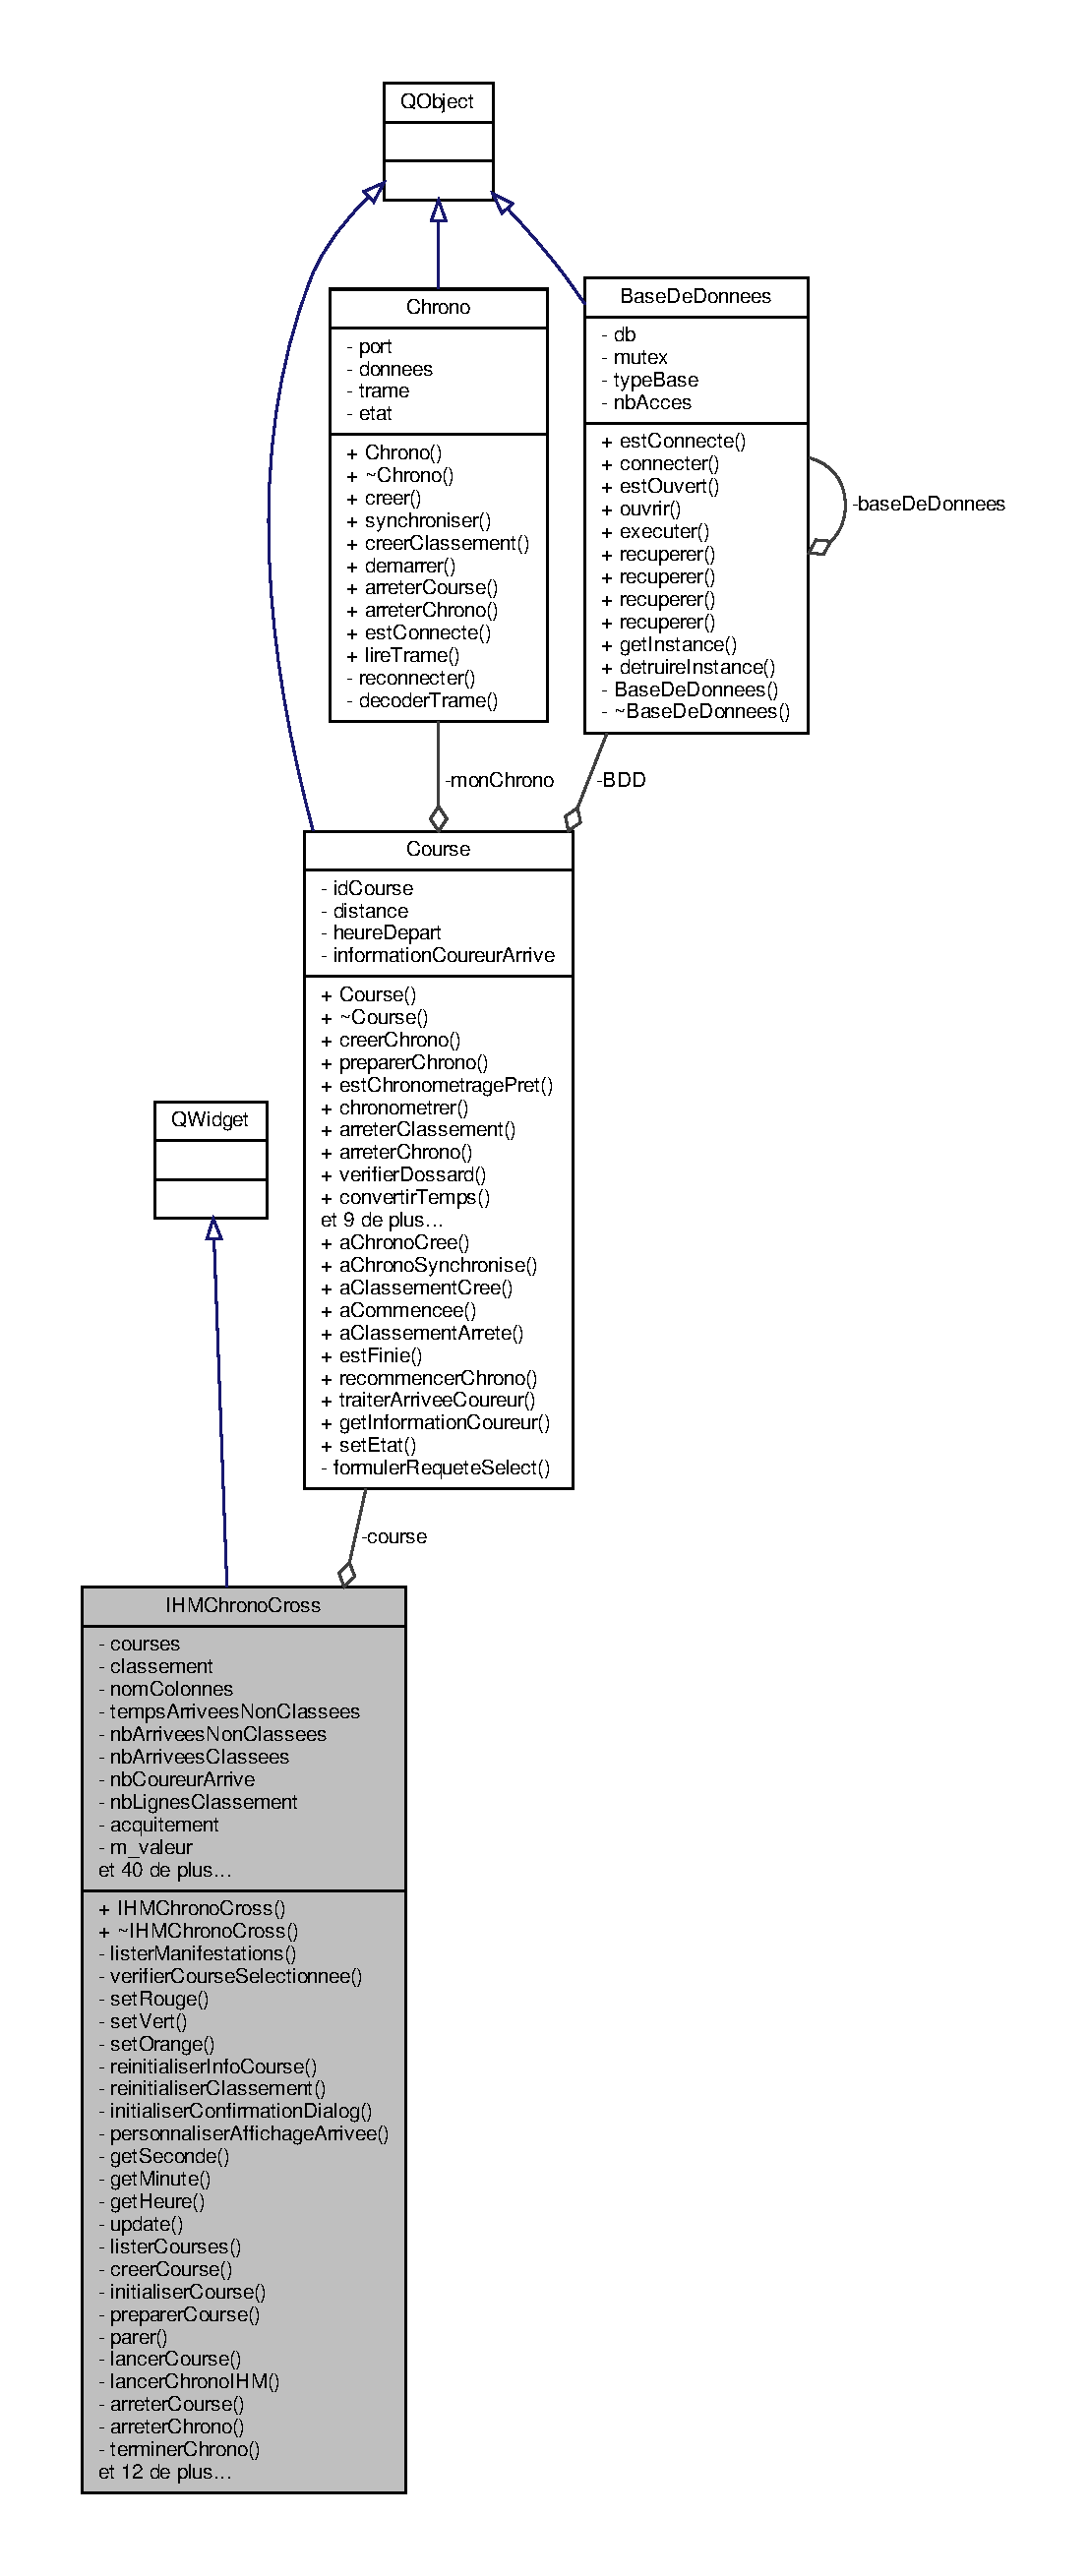
\includegraphics[height=550pt]{class_i_h_m_chrono_cross__coll__graph}
\end{center}
\end{figure}
\subsubsection*{Fonctions membres publiques}
\begin{DoxyCompactItemize}
\item 
\hyperlink{class_i_h_m_chrono_cross_a479fc90733fba3e65fb06aa4a3adc02e}{I\+H\+M\+Chrono\+Cross} (\hyperlink{class_q_widget}{Q\+Widget} $\ast$parent=nullptr)
\begin{DoxyCompactList}\small\item\em Constructeur de la fenêtre principale. \end{DoxyCompactList}\item 
\hyperlink{class_i_h_m_chrono_cross_a312f21e1d150096b3f36ba36476907eb}{$\sim$\+I\+H\+M\+Chrono\+Cross} ()
\begin{DoxyCompactList}\small\item\em Destructeur de la fenêtre principale. \end{DoxyCompactList}\end{DoxyCompactItemize}
\subsubsection*{Connecteurs privés}
\begin{DoxyCompactItemize}
\item 
void \hyperlink{class_i_h_m_chrono_cross_a1b9f117d7097b63ddabe168a5349a7e8}{lister\+Courses} (Q\+String manifestation)
\begin{DoxyCompactList}\small\item\em Méthode \hyperlink{class_i_h_m_chrono_cross_a1b9f117d7097b63ddabe168a5349a7e8}{lister\+Courses()} de la Classe \hyperlink{class_i_h_m_chrono_cross}{I\+H\+M\+Chrono\+Cross}. \end{DoxyCompactList}\item 
void \hyperlink{class_i_h_m_chrono_cross_a3fc01e539c59645e0655e56e440f4b83}{creer\+Course} (Q\+String nom\+Course)
\begin{DoxyCompactList}\small\item\em Méthode \hyperlink{class_i_h_m_chrono_cross_a3fc01e539c59645e0655e56e440f4b83}{creer\+Course()} de la classe \hyperlink{class_i_h_m_chrono_cross}{I\+H\+M\+Chrono\+Cross}. \end{DoxyCompactList}\item 
void \hyperlink{class_i_h_m_chrono_cross_adde019cc3799befac3fd9555e392eab9}{initialiser\+Course} ()
\begin{DoxyCompactList}\small\item\em S\+L\+OT \hyperlink{class_i_h_m_chrono_cross_adde019cc3799befac3fd9555e392eab9}{initialiser\+Course()} de la classe I\+H\+M\+Chrono-\/\+Cross. \end{DoxyCompactList}\item 
void \hyperlink{class_i_h_m_chrono_cross_a4926e7524f4fd76ccceb0aef5ebcb203}{preparer\+Course} ()
\begin{DoxyCompactList}\small\item\em Slots \hyperlink{class_i_h_m_chrono_cross_a4926e7524f4fd76ccceb0aef5ebcb203}{preparer\+Course()} de la classe \hyperlink{class_i_h_m_chrono_cross}{I\+H\+M\+Chrono\+Cross}. \end{DoxyCompactList}\item 
void \hyperlink{class_i_h_m_chrono_cross_aa272ffa273fc8c487ea64ef6a43b4439}{parer} ()
\begin{DoxyCompactList}\small\item\em Private S\+L\+OT \hyperlink{class_i_h_m_chrono_cross_aa272ffa273fc8c487ea64ef6a43b4439}{parer()} de la classe \hyperlink{class_i_h_m_chrono_cross}{I\+H\+M\+Chrono\+Cross}. \end{DoxyCompactList}\item 
void \hyperlink{class_i_h_m_chrono_cross_ace90922ce4c4ffeed6f1e8eb84c8c7a5}{lancer\+Course} ()
\begin{DoxyCompactList}\small\item\em S\+L\+OT \hyperlink{class_i_h_m_chrono_cross_ace90922ce4c4ffeed6f1e8eb84c8c7a5}{lancer\+Course()} de la classe \hyperlink{class_i_h_m_chrono_cross}{I\+H\+M\+Chrono\+Cross}. \end{DoxyCompactList}\item 
void \hyperlink{class_i_h_m_chrono_cross_a0e78f2d4d5e46c4551fc4517614a56d8}{lancer\+Chrono\+I\+HM} ()
\begin{DoxyCompactList}\small\item\em S\+L\+O\+TS \hyperlink{class_i_h_m_chrono_cross_a0e78f2d4d5e46c4551fc4517614a56d8}{lancer\+Chrono\+I\+H\+M()} de la classe \hyperlink{class_i_h_m_chrono_cross}{I\+H\+M\+Chrono\+Cross}. \end{DoxyCompactList}\item 
void \hyperlink{class_i_h_m_chrono_cross_ad3d8f287d08dd9aa0c6b10c9973672a4}{arreter\+Course} ()
\begin{DoxyCompactList}\small\item\em S\+L\+OT \hyperlink{class_i_h_m_chrono_cross_ad3d8f287d08dd9aa0c6b10c9973672a4}{arreter\+Course()} de la Classe \hyperlink{class_i_h_m_chrono_cross}{I\+H\+M\+Chrono\+Cross}. \end{DoxyCompactList}\item 
void \hyperlink{class_i_h_m_chrono_cross_a8d5c89a4d2ca34252acd8737e29d37fe}{arreter\+Chrono} ()
\begin{DoxyCompactList}\small\item\em S\+L\+OT \hyperlink{class_i_h_m_chrono_cross_a8d5c89a4d2ca34252acd8737e29d37fe}{arreter\+Chrono()} de la classe \hyperlink{class_i_h_m_chrono_cross}{I\+H\+M\+Chrono\+Cross}. \end{DoxyCompactList}\item 
void \hyperlink{class_i_h_m_chrono_cross_a32ee157ca6bd8c3e94b57f3cecdeee4e}{terminer\+Chrono} ()
\begin{DoxyCompactList}\small\item\em S\+L\+OT \hyperlink{class_i_h_m_chrono_cross_a32ee157ca6bd8c3e94b57f3cecdeee4e}{terminer\+Chrono()} de la classe \hyperlink{class_i_h_m_chrono_cross}{I\+H\+M\+Chrono\+Cross}. \end{DoxyCompactList}\item 
void \hyperlink{class_i_h_m_chrono_cross_ac89c6ec3040e8b787f1fbdb670405023}{terminer\+Course} ()
\begin{DoxyCompactList}\small\item\em Private S\+L\+OT \hyperlink{class_i_h_m_chrono_cross_ac89c6ec3040e8b787f1fbdb670405023}{terminer\+Course()} de la classe \hyperlink{class_i_h_m_chrono_cross}{I\+H\+M\+Chrono\+Cross}. \end{DoxyCompactList}\item 
void \hyperlink{class_i_h_m_chrono_cross_ab899a1d60c1f853b199abb937ae08e74}{commencer\+Nouvelle\+Course} ()
\begin{DoxyCompactList}\small\item\em S\+L\+OT \hyperlink{class_i_h_m_chrono_cross_ab899a1d60c1f853b199abb937ae08e74}{commencer\+Nouvelle\+Course()} de la classe \hyperlink{class_i_h_m_chrono_cross}{I\+H\+M\+Chrono\+Cross}. \end{DoxyCompactList}\item 
void \hyperlink{class_i_h_m_chrono_cross_a2ce63851d1f2723057ac649b7e320cfe}{ajouter\+Arrivee\+Coureur} (Q\+String temps\+Arrivee)
\begin{DoxyCompactList}\small\item\em S\+L\+OT \hyperlink{class_i_h_m_chrono_cross_a2ce63851d1f2723057ac649b7e320cfe}{ajouter\+Arrivee\+Coureur(\+Q\+String temps\+Arrivee)} de la classe \hyperlink{class_i_h_m_chrono_cross}{I\+H\+M\+Chrono\+Cross}. \end{DoxyCompactList}\item 
void \hyperlink{class_i_h_m_chrono_cross_a9f7f1ad130b60300a879694b6234f161}{associer\+Arrivee\+Dossard} ()
\begin{DoxyCompactList}\small\item\em S\+L\+OT \hyperlink{class_i_h_m_chrono_cross_a9f7f1ad130b60300a879694b6234f161}{associer\+Arrivee\+Dossard()} de la classe \hyperlink{class_i_h_m_chrono_cross}{I\+H\+M\+Chrono\+Cross}. \end{DoxyCompactList}\item 
void \hyperlink{class_i_h_m_chrono_cross_a5e9b561659ba63d2739335b8ab432cbf}{classer\+Arrivee} (Q\+String\+List information\+Coureur)
\begin{DoxyCompactList}\small\item\em S\+L\+OT \hyperlink{class_i_h_m_chrono_cross_a5e9b561659ba63d2739335b8ab432cbf}{classer\+Arrivee()} de la classe \hyperlink{class_i_h_m_chrono_cross}{I\+H\+M\+Chrono\+Cross}. \end{DoxyCompactList}\item 
void \hyperlink{class_i_h_m_chrono_cross_a283c721d31f90031d9a189eafb303b84}{quitter} ()
\begin{DoxyCompactList}\small\item\em S\+L\+OT \hyperlink{class_i_h_m_chrono_cross_a283c721d31f90031d9a189eafb303b84}{quitter()} de la classe \hyperlink{class_i_h_m_chrono_cross}{I\+H\+M\+Chrono\+Cross}. \end{DoxyCompactList}\item 
void \hyperlink{class_i_h_m_chrono_cross_a9706094a679e33f3595e28776596a91b}{tic} ()
\begin{DoxyCompactList}\small\item\em Méthode \hyperlink{class_i_h_m_chrono_cross_a9706094a679e33f3595e28776596a91b}{tic()} de la classe \hyperlink{class_i_h_m_chrono_cross}{I\+H\+M\+Chrono\+Cross}. \end{DoxyCompactList}\item 
void \hyperlink{class_i_h_m_chrono_cross_afe18e84e4df15c15921f2bdcfc6f4396}{afficher\+Informations\+Course} (Q\+String nom\+Course)
\begin{DoxyCompactList}\small\item\em S\+L\+OT \hyperlink{class_i_h_m_chrono_cross_afe18e84e4df15c15921f2bdcfc6f4396}{afficher\+Informations\+Course()} de la classe \hyperlink{class_i_h_m_chrono_cross}{I\+H\+M\+Chrono\+Cross}. \end{DoxyCompactList}\item 
void \hyperlink{class_i_h_m_chrono_cross_a1b23fda62742f2dd17652d3abcb33dd6}{mettre\+A\+Jour\+Nb\+Arrivees\+Non\+Classees} (int nb\+Arrivee)
\begin{DoxyCompactList}\small\item\em S\+OT \hyperlink{class_i_h_m_chrono_cross_a1b23fda62742f2dd17652d3abcb33dd6}{mettre\+A\+Jour\+Nb\+Arrivees\+Non\+Classees()} de la classe \hyperlink{class_i_h_m_chrono_cross}{I\+H\+M\+Chrono\+Cross}. \end{DoxyCompactList}\item 
void \hyperlink{class_i_h_m_chrono_cross_a3d786cb4b5c5e3a4bd566f19409601d5}{mettre\+A\+Jour\+Nb\+Arrivees\+Classees} (int nb\+Arrivee)
\begin{DoxyCompactList}\small\item\em S\+L\+OT \hyperlink{class_i_h_m_chrono_cross_a3d786cb4b5c5e3a4bd566f19409601d5}{mettre\+A\+Jour\+Nb\+Arrivees\+Classees()} de la classe \hyperlink{class_i_h_m_chrono_cross}{I\+H\+M\+Chrono\+Cross}. \end{DoxyCompactList}\item 
void \hyperlink{class_i_h_m_chrono_cross_a1e8e6d42ec7397a619940bc7bec4a6ca}{quitter\+Dialog} ()
\begin{DoxyCompactList}\small\item\em S\+L\+OT \hyperlink{class_i_h_m_chrono_cross_a1e8e6d42ec7397a619940bc7bec4a6ca}{quitter\+Dialog()} de la classe \hyperlink{class_i_h_m_chrono_cross}{I\+H\+M\+Chrono\+Cross}. \end{DoxyCompactList}\item 
void \hyperlink{class_i_h_m_chrono_cross_aca8b5d6683a3ab0018066ec16968f3f3}{supprimer\+Premier\+Temps} ()
\begin{DoxyCompactList}\small\item\em S\+L\+OT \hyperlink{class_i_h_m_chrono_cross_aca8b5d6683a3ab0018066ec16968f3f3}{supprimer\+Premier\+Temps()} de la classe \hyperlink{class_i_h_m_chrono_cross}{I\+H\+M\+Chrono\+Cross}. \end{DoxyCompactList}\end{DoxyCompactItemize}
\subsubsection*{Fonctions membres privées}
\begin{DoxyCompactItemize}
\item 
void \hyperlink{class_i_h_m_chrono_cross_adb47e6ee9c2a917a6df77b64930c3c48}{lister\+Manifestations} ()
\begin{DoxyCompactList}\small\item\em Méthode \hyperlink{class_i_h_m_chrono_cross_adb47e6ee9c2a917a6df77b64930c3c48}{lister\+Manifestations()} de la Classe \hyperlink{class_i_h_m_chrono_cross}{I\+H\+M\+Chrono\+Cross}. \end{DoxyCompactList}\item 
bool \hyperlink{class_i_h_m_chrono_cross_afa7d1fb0245bb3e8bbffdf2687b02248}{verifier\+Course\+Selectionnee} (Q\+String course\+Selectionnee)
\begin{DoxyCompactList}\small\item\em Méthode \hyperlink{class_i_h_m_chrono_cross_afa7d1fb0245bb3e8bbffdf2687b02248}{verifier\+Course\+Selectionnee()} de la classe \hyperlink{class_i_h_m_chrono_cross}{I\+H\+M\+Chrono\+Cross}. \end{DoxyCompactList}\item 
void \hyperlink{class_i_h_m_chrono_cross_a3b46a31326bdde2b5ad67a9f0a6de76b}{set\+Rouge} (Q\+Label $\ast$label)
\begin{DoxyCompactList}\small\item\em Méthode \hyperlink{class_i_h_m_chrono_cross_a3b46a31326bdde2b5ad67a9f0a6de76b}{set\+Rouge()} de la classe \hyperlink{class_i_h_m_chrono_cross}{I\+H\+M\+Chrono\+Cross}. \end{DoxyCompactList}\item 
void \hyperlink{class_i_h_m_chrono_cross_aba2b1a136332baa7bd4905f9af15705b}{set\+Vert} (Q\+Label $\ast$label)
\begin{DoxyCompactList}\small\item\em Méthode \hyperlink{class_i_h_m_chrono_cross_aba2b1a136332baa7bd4905f9af15705b}{set\+Vert()} de la classe \hyperlink{class_i_h_m_chrono_cross}{I\+H\+M\+Chrono\+Cross}. \end{DoxyCompactList}\item 
void \hyperlink{class_i_h_m_chrono_cross_a7e2424925f588d7a1914befc3c6c832e}{set\+Orange} (Q\+Label $\ast$label)
\begin{DoxyCompactList}\small\item\em Méthode \hyperlink{class_i_h_m_chrono_cross_a7e2424925f588d7a1914befc3c6c832e}{set\+Orange()} de la classe \hyperlink{class_i_h_m_chrono_cross}{I\+H\+M\+Chrono\+Cross}. \end{DoxyCompactList}\item 
void \hyperlink{class_i_h_m_chrono_cross_a1149f4f57c8cf34048f93fba6b4176b3}{reinitialiser\+Info\+Course} ()
\begin{DoxyCompactList}\small\item\em Méthode \hyperlink{class_i_h_m_chrono_cross_a1149f4f57c8cf34048f93fba6b4176b3}{reinitialiser\+Info\+Course()} de la classe \hyperlink{class_i_h_m_chrono_cross}{I\+H\+M\+Chrono\+Cross}. \end{DoxyCompactList}\item 
void \hyperlink{class_i_h_m_chrono_cross_aaf8fa3bf16956fd0e0ceeab6e65f6741}{reinitialiser\+Classement} ()
\begin{DoxyCompactList}\small\item\em Méthode \hyperlink{class_i_h_m_chrono_cross_aaf8fa3bf16956fd0e0ceeab6e65f6741}{reinitialiser\+Classement()} de la classe \hyperlink{class_i_h_m_chrono_cross}{I\+H\+M\+Chrono\+Cross}. \end{DoxyCompactList}\item 
void \hyperlink{class_i_h_m_chrono_cross_a866a247fad23eca2af31ed985afe7cd3}{initialiser\+Confirmation\+Dialog} ()
\begin{DoxyCompactList}\small\item\em Méthode \hyperlink{class_i_h_m_chrono_cross_a866a247fad23eca2af31ed985afe7cd3}{initialiser\+Confirmation\+Dialog()} de la classe \hyperlink{class_i_h_m_chrono_cross}{I\+H\+M\+Chrono\+Cross}. \end{DoxyCompactList}\item 
void \hyperlink{class_i_h_m_chrono_cross_a41c2ff49d25069f8dfa2a7b3d0606d38}{personnaliser\+Affichage\+Arrivee} (int \hyperlink{class_i_h_m_chrono_cross_a86ed3469ca99988211bcf0970527c119}{nb\+Lignes\+Classement})
\begin{DoxyCompactList}\small\item\em Méthode \hyperlink{class_i_h_m_chrono_cross_a41c2ff49d25069f8dfa2a7b3d0606d38}{personnaliser\+Affichage\+Arrivee()} de la classe \hyperlink{class_i_h_m_chrono_cross}{I\+H\+M\+Chrono\+Cross}. \end{DoxyCompactList}\item 
long \hyperlink{class_i_h_m_chrono_cross_a0dfb2dc2b85937b1f218584ce84e9d98}{get\+Seconde} ()
\begin{DoxyCompactList}\small\item\em Méthode \hyperlink{class_i_h_m_chrono_cross_a0dfb2dc2b85937b1f218584ce84e9d98}{get\+Seconde()} de la classe \hyperlink{class_i_h_m_chrono_cross}{I\+H\+M\+Chrono\+Cross}. \end{DoxyCompactList}\item 
long \hyperlink{class_i_h_m_chrono_cross_a0cee9742e561398390bedb29ef7d6258}{get\+Minute} ()
\begin{DoxyCompactList}\small\item\em Méthode \hyperlink{class_i_h_m_chrono_cross_a0cee9742e561398390bedb29ef7d6258}{get\+Minute()} de la classe \hyperlink{class_i_h_m_chrono_cross}{I\+H\+M\+Chrono\+Cross}. \end{DoxyCompactList}\item 
long \hyperlink{class_i_h_m_chrono_cross_a42054b4d5246c939bf0f621edb0e1aae}{get\+Heure} ()
\begin{DoxyCompactList}\small\item\em Méthode \hyperlink{class_i_h_m_chrono_cross_a42054b4d5246c939bf0f621edb0e1aae}{get\+Heure()} de la classe \hyperlink{class_i_h_m_chrono_cross}{I\+H\+M\+Chrono\+Cross}. \end{DoxyCompactList}\item 
void \hyperlink{class_i_h_m_chrono_cross_a2cc8b686168528ab0d642a0cba6e1c5a}{update} ()
\begin{DoxyCompactList}\small\item\em Méthode \hyperlink{class_i_h_m_chrono_cross_a2cc8b686168528ab0d642a0cba6e1c5a}{update()} de la classe \hyperlink{class_i_h_m_chrono_cross}{I\+H\+M\+Chrono\+Cross}. \end{DoxyCompactList}\end{DoxyCompactItemize}
\subsubsection*{Attributs privés}
\begin{DoxyCompactItemize}
\item 
\hyperlink{class_course}{Course} $\ast$ \hyperlink{class_i_h_m_chrono_cross_a03a8226c0e7f423d29302d9a06284ab4}{course}
\begin{DoxyCompactList}\small\item\em agrégation d\textquotesingle{}une course \end{DoxyCompactList}\item 
Q\+Vector$<$ Q\+String\+List $>$ \hyperlink{class_i_h_m_chrono_cross_a646f70038327c068a2f7c7be6e07d2ee}{courses}
\begin{DoxyCompactList}\small\item\em liste des courses pour une manifestation \end{DoxyCompactList}\item 
Q\+String\+List \hyperlink{class_i_h_m_chrono_cross_a49236628e14e516e1ab7a181eac8fea8}{classement}
\begin{DoxyCompactList}\small\item\em Liste du classement pour une course. \end{DoxyCompactList}\item 
Q\+String\+List \hyperlink{class_i_h_m_chrono_cross_a21f1b0ba82ff1b4a7b842b5f3c411e60}{nom\+Colonnes}
\begin{DoxyCompactList}\small\item\em Liste de nom des colonnes du classement \char`\"{}\+Temps, dossard, nom...\char`\"{}. \end{DoxyCompactList}\item 
Q\+String\+List \hyperlink{class_i_h_m_chrono_cross_a9d0542a5334cd284d1ea9cf732cb013e}{temps\+Arrivees\+Non\+Classees}
\begin{DoxyCompactList}\small\item\em Liste des arrivées non classés. \end{DoxyCompactList}\item 
int \hyperlink{class_i_h_m_chrono_cross_aa3198d36b0574b477a328621c8e1e0f0}{nb\+Arrivees\+Non\+Classees}
\item 
int \hyperlink{class_i_h_m_chrono_cross_a9bdcd0e57b79f64957eefea0f9d2b097}{nb\+Arrivees\+Classees}
\item 
int \hyperlink{class_i_h_m_chrono_cross_aba349505e99e6e320b218ba2b7fb485e}{nb\+Coureur\+Arrive}
\begin{DoxyCompactList}\small\item\em Nombre de coureurs arrivés. \end{DoxyCompactList}\item 
int \hyperlink{class_i_h_m_chrono_cross_a86ed3469ca99988211bcf0970527c119}{nb\+Lignes\+Classement}
\begin{DoxyCompactList}\small\item\em nombre de lignes du classement \end{DoxyCompactList}\item 
bool \hyperlink{class_i_h_m_chrono_cross_a3ad2d6f9520ae7ed917fba070ed55d4c}{acquitement}
\item 
long \hyperlink{class_i_h_m_chrono_cross_a4bb2449f0b2cc9891c09fa3e32f56229}{m\+\_\+valeur}
\begin{DoxyCompactList}\small\item\em Valeur du chrono. \end{DoxyCompactList}\item 
Q\+Combo\+Box $\ast$ \hyperlink{class_i_h_m_chrono_cross_a4b7a6af527d8d2d28d8ea6ea7cbfac75}{cb\+Liste\+Manifestations}
\begin{DoxyCompactList}\small\item\em Combobox contenant les différentes manifesations de la base de donnée. \end{DoxyCompactList}\item 
Q\+Combo\+Box $\ast$ \hyperlink{class_i_h_m_chrono_cross_af47891e3e9f2bb2c955be8c128e830b5}{cb\+Liste\+Courses}
\begin{DoxyCompactList}\small\item\em Combobox contenant les différentes course de la base de donnée. \end{DoxyCompactList}\item 
Q\+Label $\ast$ \hyperlink{class_i_h_m_chrono_cross_a7430cf36cc48d17297ddc03fe69e9b72}{label\+Manifestations}
\begin{DoxyCompactList}\small\item\em Label contenant le Q\+String \char`\"{}\+Manifestations \+: \char`\"{} devant cb\+Liste\+Manifestations. \end{DoxyCompactList}\item 
Q\+Label $\ast$ \hyperlink{class_i_h_m_chrono_cross_a2b563f2574ad86acaecc01f0357f85be}{label\+Liste\+Courses}
\begin{DoxyCompactList}\small\item\em Label contenant le Q\+String \char`\"{}\+Courses \+: \char`\"{} devant cb\+Liste\+Courses. \end{DoxyCompactList}\item 
Q\+Label $\ast$ \hyperlink{class_i_h_m_chrono_cross_a73afea901ae4b6eb4c0d136818ed1fa6}{label\+Numero\+Dossard}
\begin{DoxyCompactList}\small\item\em Label contenant le Q\+String \char`\"{}\+N° dossard \+: \char`\"{}. \end{DoxyCompactList}\item 
Q\+Label $\ast$ \hyperlink{class_i_h_m_chrono_cross_a7684bc78d49abe63f021ee623bea575e}{label\+Zone\+Course}
\begin{DoxyCompactList}\small\item\em Label contenant le texte \+: \hyperlink{class_course}{Course} symbolisant la zone course. \end{DoxyCompactList}\item 
Q\+Label $\ast$ \hyperlink{class_i_h_m_chrono_cross_ac07ff8651a5a929f8847fa85eef9fe89}{label\+Zone\+Classement}
\begin{DoxyCompactList}\small\item\em Label contenant le texte \+: Classement symbolisant la zone classement. \end{DoxyCompactList}\item 
Q\+Label $\ast$ \hyperlink{class_i_h_m_chrono_cross_ad28922f5316673a1e181747879ef6855}{label\+Zone\+Chrono}
\begin{DoxyCompactList}\small\item\em Label contenant le texte \char`\"{}\+Chrono \+: \char`\"{} symbolisant la zone chrono. \end{DoxyCompactList}\item 
Q\+Label $\ast$ \hyperlink{class_i_h_m_chrono_cross_a76f2f83c624da73e3d3de6a8b4ff43a1}{logo\+Chrono\+Cross}
\begin{DoxyCompactList}\small\item\em Label contenant l\textquotesingle{}image du logo Chrono-\/\+Cross. \end{DoxyCompactList}\item 
Q\+Label $\ast$ \hyperlink{class_i_h_m_chrono_cross_ad247dfd005cb835c90aca67b1384578b}{label\+Etat\+Chrono}
\begin{DoxyCompactList}\small\item\em Label contenant le texte \char`\"{}\+Etat \+: \char`\"{} pour la led chrono. \end{DoxyCompactList}\item 
Q\+Label $\ast$ \hyperlink{class_i_h_m_chrono_cross_ad43bab2d9a06fe2fb198c56d8b9faab2}{label\+Led\+Chrono}
\begin{DoxyCompactList}\small\item\em Label contenant la L\+ED (état vert, orange ou rouge) qui représente l\textquotesingle{}état de la connexion avec le T\+AG H\+E\+U\+ER. \end{DoxyCompactList}\item 
Q\+Label $\ast$ \hyperlink{class_i_h_m_chrono_cross_a8568c80f2e2ffe96c81d2a94a2146159}{label\+Led\+Course}
\begin{DoxyCompactList}\small\item\em Label contenant la L\+ED (état vert, orange ou rouge) qui représente l\textquotesingle{}état du chrono, si il est prêt à faire une course. \end{DoxyCompactList}\item 
Q\+Label $\ast$ \hyperlink{class_i_h_m_chrono_cross_a433796aedfcc26313f639bd5157b1135}{label\+Etat\+Course}
\begin{DoxyCompactList}\small\item\em Label contenant le texte \char`\"{}\+Etat \+: \char`\"{} pour la led course. \end{DoxyCompactList}\item 
Q\+Label $\ast$ \hyperlink{class_i_h_m_chrono_cross_a56f6c02a8d3274c4359f12709cefa5d2}{label\+Zone\+Arrivees}
\begin{DoxyCompactList}\small\item\em Label contenant le Q\+String \char`\"{}\+Arrivées \+: \char`\"{} symbolisant la zone des arrivées non classées. \end{DoxyCompactList}\item 
Q\+Label $\ast$ \hyperlink{class_i_h_m_chrono_cross_abd23647486d38e6f57aef1faf50757af}{label\+Message\+Dossard}
\begin{DoxyCompactList}\small\item\em Label du message d\textquotesingle{}érreur pour les numéros de dossards. \end{DoxyCompactList}\item 
Q\+Label $\ast$ \hyperlink{class_i_h_m_chrono_cross_a6d818ff507406ebf299c571e0e5c1e49}{label\+Message\+Supprimer}
\begin{DoxyCompactList}\small\item\em label contenant le message d\textquotesingle{}information pour supprimer le premier temps non classée \end{DoxyCompactList}\item 
Q\+Label $\ast$ \hyperlink{class_i_h_m_chrono_cross_a9d410e8bc161481a83298176b2702519}{label\+Nb\+Inscrit}
\begin{DoxyCompactList}\small\item\em Label contentant le texte \char`\"{}\+Nombre d\textquotesingle{}inscrit \+:\char`\"{}. \end{DoxyCompactList}\item 
Q\+Label $\ast$ \hyperlink{class_i_h_m_chrono_cross_a3249b3528e5b75353bb8fb80d27eefe3}{label\+Nb\+Arrivees\+Non\+Classees}
\begin{DoxyCompactList}\small\item\em Label contentant le texte \char`\"{}\+Nombre d\textquotesingle{}arrivées non classées \+:\char`\"{}. \end{DoxyCompactList}\item 
Q\+Label $\ast$ \hyperlink{class_i_h_m_chrono_cross_a08fd415de59fe6f42663f3f36f074e61}{label\+Nb\+Arrivees\+Classees}
\begin{DoxyCompactList}\small\item\em Label contentant le texte \char`\"{}\+Nombre d\textquotesingle{}arrivées classées \+:\char`\"{}. \end{DoxyCompactList}\item 
Q\+L\+C\+D\+Number $\ast$ \hyperlink{class_i_h_m_chrono_cross_a9cf1b999b13e69fdd0fb11ddb9011ed5}{Q\+L\+C\+D\+Nb\+Arrivees\+Non\+Classees}
\begin{DoxyCompactList}\small\item\em Q\+L\+CD qui affiche le nombre d\textquotesingle{}arrivées non classées. \end{DoxyCompactList}\item 
Q\+L\+C\+D\+Number $\ast$ \hyperlink{class_i_h_m_chrono_cross_aeba189eacad7e19e009ae4764f98b9be}{Q\+L\+C\+D\+Nb\+Arrivees\+Classees}
\begin{DoxyCompactList}\small\item\em Q\+L\+CD qui affiche le nombre d\textquotesingle{}arrivées classées. \end{DoxyCompactList}\item 
Q\+Label $\ast$ \hyperlink{class_i_h_m_chrono_cross_aebe86f4e614f568db5558bf99f1b44e6}{label\+Nom\+Course}
\item 
Q\+Label $\ast$ \hyperlink{class_i_h_m_chrono_cross_a4748740a4973bf62c408be380ac0ae77}{label\+Distance\+Course}
\item 
Q\+Label $\ast$ \hyperlink{class_i_h_m_chrono_cross_ad071b8c6ecc126fca3e17e58e83942d9}{label\+Heure\+Course}
\item 
Q\+L\+C\+D\+Number $\ast$ \hyperlink{class_i_h_m_chrono_cross_a6169c1483faab14d1f619d1d838c198e}{Q\+L\+C\+D\+Chrono}
\begin{DoxyCompactList}\small\item\em Q\+L\+CD contenant le chrono. \end{DoxyCompactList}\item 
Q\+Line\+Edit $\ast$ \hyperlink{class_i_h_m_chrono_cross_ad2e156ff9412644debf8da7a3ec1566d}{line\+Edit\+Numero\+Dossard}
\begin{DoxyCompactList}\small\item\em Line\+Edit qui permet de rentrer un numéro de dossard. \end{DoxyCompactList}\item 
Q\+Push\+Button $\ast$ \hyperlink{class_i_h_m_chrono_cross_aaef501bd1190a5ec06a214d3265b8c0b}{b\+Synchroniser}
\begin{DoxyCompactList}\small\item\em Bouton Synchroniser. \end{DoxyCompactList}\item 
Q\+Push\+Button $\ast$ \hyperlink{class_i_h_m_chrono_cross_a1b0a7c5e58d6a9f873cdc912d67b8de9}{b\+Lancer}
\begin{DoxyCompactList}\small\item\em Bouton Lancer le chronomètre. \end{DoxyCompactList}\item 
Q\+Push\+Button $\ast$ \hyperlink{class_i_h_m_chrono_cross_a75ce4fcdab11095834fe3f9e931f8964}{b\+Arreter}
\begin{DoxyCompactList}\small\item\em Bouton Arreter. \end{DoxyCompactList}\item 
Q\+Push\+Button $\ast$ \hyperlink{class_i_h_m_chrono_cross_a63721ec2d7d51b11b164b4502ace8262}{b\+Terminer}
\begin{DoxyCompactList}\small\item\em Bouton Terminer. \end{DoxyCompactList}\item 
Q\+Push\+Button $\ast$ \hyperlink{class_i_h_m_chrono_cross_aec2458a0c2ff0d2c37fa409fb8e99ce7}{b\+Associer}
\begin{DoxyCompactList}\small\item\em Bouton Associer. \end{DoxyCompactList}\item 
Q\+Table\+View $\ast$ \hyperlink{class_i_h_m_chrono_cross_a199204276756844adbd6ca3c9030ad2f}{vue\+Tableau\+Classement}
\begin{DoxyCompactList}\small\item\em Vue en liste classement. \end{DoxyCompactList}\item 
Q\+Standard\+Item\+Model $\ast$ \hyperlink{class_i_h_m_chrono_cross_ac25c95280801f36c43a1c41cf2fa253e}{modele\+Classement}
\begin{DoxyCompactList}\small\item\em Model du classement. \end{DoxyCompactList}\item 
Q\+List\+View $\ast$ \hyperlink{class_i_h_m_chrono_cross_aaf04338d882f708e57d9872b1c82b7a0}{vue\+Liste\+Temps\+Arrivees\+Non\+Classees}
\begin{DoxyCompactList}\small\item\em Vue en tableau des temps non classés. \end{DoxyCompactList}\item 
Q\+String\+List\+Model $\ast$ \hyperlink{class_i_h_m_chrono_cross_a12a210c6a93f70df764841b7d322b05c}{modele\+Arrivees\+Non\+Classees}
\begin{DoxyCompactList}\small\item\em Model des arrivées non classés. \end{DoxyCompactList}\item 
Q\+Timer $\ast$ \hyperlink{class_i_h_m_chrono_cross_ad29ebde513a6e722cf87aa06e767416a}{m\+\_\+timer}
\begin{DoxyCompactList}\small\item\em \hyperlink{class_chrono}{Chrono} de l\textquotesingle{}ihm. \end{DoxyCompactList}\item 
Q\+Dialog $\ast$ \hyperlink{class_i_h_m_chrono_cross_ad7fc4afa5689501063cc207a8daf5752}{confirmation\+Dialog}
\item 
Q\+Label $\ast$ \hyperlink{class_i_h_m_chrono_cross_a20522f998469b4b34b8939dce6b239b3}{label\+Confirmation\+Dialog}
\item 
Q\+Push\+Button $\ast$ \hyperlink{class_i_h_m_chrono_cross_a57bb61d8175dc09f0497ee3834cb6ad5}{b\+Confirmation\+Dialog}
\item 
Q\+Push\+Button $\ast$ \hyperlink{class_i_h_m_chrono_cross_a7d2639da4d7d7afae5d2a66e83695a4e}{b\+Annuler\+Dialog}
\end{DoxyCompactItemize}


\subsubsection{Description détaillée}
La fenêtre principale de l\textquotesingle{}application Chrono-\/\+Cross. 

\begin{DoxyAuthor}{Auteur}
A\+N\+D\+R\+EO Michaël 
\end{DoxyAuthor}
\begin{DoxyVersion}{Version}
1.\+1 
\end{DoxyVersion}


\subsubsection{Documentation des constructeurs et destructeur}
\mbox{\Hypertarget{class_i_h_m_chrono_cross_a479fc90733fba3e65fb06aa4a3adc02e}\label{class_i_h_m_chrono_cross_a479fc90733fba3e65fb06aa4a3adc02e}} 
\index{I\+H\+M\+Chrono\+Cross@{I\+H\+M\+Chrono\+Cross}!I\+H\+M\+Chrono\+Cross@{I\+H\+M\+Chrono\+Cross}}
\index{I\+H\+M\+Chrono\+Cross@{I\+H\+M\+Chrono\+Cross}!I\+H\+M\+Chrono\+Cross@{I\+H\+M\+Chrono\+Cross}}
\paragraph{\texorpdfstring{I\+H\+M\+Chrono\+Cross()}{IHMChronoCross()}}
{\footnotesize\ttfamily I\+H\+M\+Chrono\+Cross\+::\+I\+H\+M\+Chrono\+Cross (\begin{DoxyParamCaption}\item[{\hyperlink{class_q_widget}{Q\+Widget} $\ast$}]{parent = {\ttfamily nullptr} }\end{DoxyParamCaption})}



Constructeur de la fenêtre principale. 


\begin{DoxyParams}{Paramètres}
{\em parent} & \hyperlink{class_q_object}{Q\+Object} Adresse de l\textquotesingle{}objet Qt parent (0 = pas de parent car c\textquotesingle{}est la fenêtre principale) \\
\hline
\end{DoxyParams}


Références \hyperlink{class_i_h_m_chrono_cross_afe18e84e4df15c15921f2bdcfc6f4396}{afficher\+Informations\+Course()}, \hyperlink{class_i_h_m_chrono_cross_a2ce63851d1f2723057ac649b7e320cfe}{ajouter\+Arrivee\+Coureur()}, \hyperlink{class_i_h_m_chrono_cross_a8d5c89a4d2ca34252acd8737e29d37fe}{arreter\+Chrono()}, \hyperlink{class_i_h_m_chrono_cross_ad3d8f287d08dd9aa0c6b10c9973672a4}{arreter\+Course()}, \hyperlink{class_i_h_m_chrono_cross_a9f7f1ad130b60300a879694b6234f161}{associer\+Arrivee\+Dossard()}, \hyperlink{class_i_h_m_chrono_cross_a75ce4fcdab11095834fe3f9e931f8964}{b\+Arreter}, \hyperlink{class_i_h_m_chrono_cross_aec2458a0c2ff0d2c37fa409fb8e99ce7}{b\+Associer}, \hyperlink{class_i_h_m_chrono_cross_a1b0a7c5e58d6a9f873cdc912d67b8de9}{b\+Lancer}, \hyperlink{class_i_h_m_chrono_cross_aaef501bd1190a5ec06a214d3265b8c0b}{b\+Synchroniser}, \hyperlink{class_i_h_m_chrono_cross_a63721ec2d7d51b11b164b4502ace8262}{b\+Terminer}, \hyperlink{class_i_h_m_chrono_cross_af47891e3e9f2bb2c955be8c128e830b5}{cb\+Liste\+Courses}, \hyperlink{class_i_h_m_chrono_cross_a4b7a6af527d8d2d28d8ea6ea7cbfac75}{cb\+Liste\+Manifestations}, \hyperlink{class_i_h_m_chrono_cross_a49236628e14e516e1ab7a181eac8fea8}{classement}, \hyperlink{class_i_h_m_chrono_cross_a5e9b561659ba63d2739335b8ab432cbf}{classer\+Arrivee()}, \hyperlink{class_i_h_m_chrono_cross_ab899a1d60c1f853b199abb937ae08e74}{commencer\+Nouvelle\+Course()}, \hyperlink{class_i_h_m_chrono_cross_a03a8226c0e7f423d29302d9a06284ab4}{course}, \hyperlink{class_i_h_m_chrono_cross_a3fc01e539c59645e0655e56e440f4b83}{creer\+Course()}, \hyperlink{class_course_ad8dd87e7f299bc938f40423f28c837e8}{Course\+::get\+Nb\+Arrivee()}, \hyperlink{ihmchronocross_8h_aa8bee638aa78f9b332485225ecc8e75e}{I\+M\+A\+G\+E\+C\+H\+R\+O\+N\+O\+C\+R\+O\+SS}, \hyperlink{class_i_h_m_chrono_cross_adde019cc3799befac3fd9555e392eab9}{initialiser\+Course()}, \hyperlink{class_i_h_m_chrono_cross_a4748740a4973bf62c408be380ac0ae77}{label\+Distance\+Course}, \hyperlink{class_i_h_m_chrono_cross_ad247dfd005cb835c90aca67b1384578b}{label\+Etat\+Chrono}, \hyperlink{class_i_h_m_chrono_cross_a433796aedfcc26313f639bd5157b1135}{label\+Etat\+Course}, \hyperlink{class_i_h_m_chrono_cross_ad071b8c6ecc126fca3e17e58e83942d9}{label\+Heure\+Course}, \hyperlink{class_i_h_m_chrono_cross_ad43bab2d9a06fe2fb198c56d8b9faab2}{label\+Led\+Chrono}, \hyperlink{class_i_h_m_chrono_cross_a8568c80f2e2ffe96c81d2a94a2146159}{label\+Led\+Course}, \hyperlink{class_i_h_m_chrono_cross_a2b563f2574ad86acaecc01f0357f85be}{label\+Liste\+Courses}, \hyperlink{class_i_h_m_chrono_cross_a7430cf36cc48d17297ddc03fe69e9b72}{label\+Manifestations}, \hyperlink{class_i_h_m_chrono_cross_abd23647486d38e6f57aef1faf50757af}{label\+Message\+Dossard}, \hyperlink{class_i_h_m_chrono_cross_a6d818ff507406ebf299c571e0e5c1e49}{label\+Message\+Supprimer}, \hyperlink{class_i_h_m_chrono_cross_a08fd415de59fe6f42663f3f36f074e61}{label\+Nb\+Arrivees\+Classees}, \hyperlink{class_i_h_m_chrono_cross_a3249b3528e5b75353bb8fb80d27eefe3}{label\+Nb\+Arrivees\+Non\+Classees}, \hyperlink{class_i_h_m_chrono_cross_a9d410e8bc161481a83298176b2702519}{label\+Nb\+Inscrit}, \hyperlink{class_i_h_m_chrono_cross_aebe86f4e614f568db5558bf99f1b44e6}{label\+Nom\+Course}, \hyperlink{class_i_h_m_chrono_cross_a73afea901ae4b6eb4c0d136818ed1fa6}{label\+Numero\+Dossard}, \hyperlink{class_i_h_m_chrono_cross_a56f6c02a8d3274c4359f12709cefa5d2}{label\+Zone\+Arrivees}, \hyperlink{class_i_h_m_chrono_cross_ad28922f5316673a1e181747879ef6855}{label\+Zone\+Chrono}, \hyperlink{class_i_h_m_chrono_cross_ac07ff8651a5a929f8847fa85eef9fe89}{label\+Zone\+Classement}, \hyperlink{class_i_h_m_chrono_cross_a7684bc78d49abe63f021ee623bea575e}{label\+Zone\+Course}, \hyperlink{class_i_h_m_chrono_cross_a0e78f2d4d5e46c4551fc4517614a56d8}{lancer\+Chrono\+I\+H\+M()}, \hyperlink{class_i_h_m_chrono_cross_ace90922ce4c4ffeed6f1e8eb84c8c7a5}{lancer\+Course()}, \hyperlink{class_i_h_m_chrono_cross_ad2e156ff9412644debf8da7a3ec1566d}{line\+Edit\+Numero\+Dossard}, \hyperlink{class_i_h_m_chrono_cross_a1b9f117d7097b63ddabe168a5349a7e8}{lister\+Courses()}, \hyperlink{class_i_h_m_chrono_cross_adb47e6ee9c2a917a6df77b64930c3c48}{lister\+Manifestations()}, \hyperlink{class_i_h_m_chrono_cross_a76f2f83c624da73e3d3de6a8b4ff43a1}{logo\+Chrono\+Cross}, \hyperlink{class_i_h_m_chrono_cross_ad29ebde513a6e722cf87aa06e767416a}{m\+\_\+timer}, \hyperlink{class_i_h_m_chrono_cross_a4bb2449f0b2cc9891c09fa3e32f56229}{m\+\_\+valeur}, \hyperlink{class_i_h_m_chrono_cross_a12a210c6a93f70df764841b7d322b05c}{modele\+Arrivees\+Non\+Classees}, \hyperlink{class_i_h_m_chrono_cross_ac25c95280801f36c43a1c41cf2fa253e}{modele\+Classement}, \hyperlink{class_i_h_m_chrono_cross_a9bdcd0e57b79f64957eefea0f9d2b097}{nb\+Arrivees\+Classees}, \hyperlink{class_i_h_m_chrono_cross_aa3198d36b0574b477a328621c8e1e0f0}{nb\+Arrivees\+Non\+Classees}, \hyperlink{class_i_h_m_chrono_cross_aba349505e99e6e320b218ba2b7fb485e}{nb\+Coureur\+Arrive}, \hyperlink{class_i_h_m_chrono_cross_a86ed3469ca99988211bcf0970527c119}{nb\+Lignes\+Classement}, \hyperlink{class_i_h_m_chrono_cross_a21f1b0ba82ff1b4a7b842b5f3c411e60}{nom\+Colonnes}, \hyperlink{class_i_h_m_chrono_cross_aa272ffa273fc8c487ea64ef6a43b4439}{parer()}, \hyperlink{class_i_h_m_chrono_cross_a4926e7524f4fd76ccceb0aef5ebcb203}{preparer\+Course()}, \hyperlink{class_i_h_m_chrono_cross_a6169c1483faab14d1f619d1d838c198e}{Q\+L\+C\+D\+Chrono}, \hyperlink{class_i_h_m_chrono_cross_aeba189eacad7e19e009ae4764f98b9be}{Q\+L\+C\+D\+Nb\+Arrivees\+Classees}, \hyperlink{class_i_h_m_chrono_cross_a9cf1b999b13e69fdd0fb11ddb9011ed5}{Q\+L\+C\+D\+Nb\+Arrivees\+Non\+Classees}, \hyperlink{class_i_h_m_chrono_cross_a283c721d31f90031d9a189eafb303b84}{quitter()}, \hyperlink{class_i_h_m_chrono_cross_a3b46a31326bdde2b5ad67a9f0a6de76b}{set\+Rouge()}, \hyperlink{ihmchronocross_8h_a93c1a7628e080979c2ae8f83b6c69606}{T\+A\+I\+L\+L\+E\+T\+E\+X\+T\+E\+B\+U\+T\+ON}, \hyperlink{ihmchronocross_8h_a93033547a126f30c05119d40b51384da}{T\+A\+I\+L\+L\+E\+T\+E\+X\+T\+E\+I\+N\+FO}, \hyperlink{ihmchronocross_8h_a407f067284fd7ac16426ac29cbfcd356}{T\+A\+I\+L\+L\+E\+T\+E\+X\+T\+E\+L\+A\+B\+EL}, \hyperlink{ihmchronocross_8h_a4169235bca6fe9370d9b368912e62af0}{T\+A\+I\+L\+L\+E\+T\+E\+X\+T\+E\+L\+I\+S\+TE}, \hyperlink{ihmchronocross_8h_a79ebe381f5864a987975ff0072b37ae7}{T\+A\+I\+L\+L\+E\+T\+E\+X\+T\+E\+S\+U\+P\+P\+R\+I\+M\+ER}, \hyperlink{class_i_h_m_chrono_cross_a32ee157ca6bd8c3e94b57f3cecdeee4e}{terminer\+Chrono()}, \hyperlink{class_i_h_m_chrono_cross_ac89c6ec3040e8b787f1fbdb670405023}{terminer\+Course()}, \hyperlink{class_i_h_m_chrono_cross_a9706094a679e33f3595e28776596a91b}{tic()}, \hyperlink{class_i_h_m_chrono_cross_aaf04338d882f708e57d9872b1c82b7a0}{vue\+Liste\+Temps\+Arrivees\+Non\+Classees}, et \hyperlink{class_i_h_m_chrono_cross_a199204276756844adbd6ca3c9030ad2f}{vue\+Tableau\+Classement}.


\begin{DoxyCode}
00017                                               : \hyperlink{class_q_widget}{QWidget}(parent)
00018 \{
00019 
00020     \hyperlink{class_i_h_m_chrono_cross_a03a8226c0e7f423d29302d9a06284ab4}{course} = \textcolor{keyword}{new} \hyperlink{class_course}{Course}(\textcolor{keyword}{this});
00021 
00022     \hyperlink{class_i_h_m_chrono_cross_aba349505e99e6e320b218ba2b7fb485e}{nbCoureurArrive} = \hyperlink{class_i_h_m_chrono_cross_a03a8226c0e7f423d29302d9a06284ab4}{course}->\hyperlink{class_course_ad8dd87e7f299bc938f40423f28c837e8}{getNbArrivee}();
00023     \hyperlink{class_i_h_m_chrono_cross_aa3198d36b0574b477a328621c8e1e0f0}{nbArriveesNonClassees} = 0;
00024     \hyperlink{class_i_h_m_chrono_cross_a9bdcd0e57b79f64957eefea0f9d2b097}{nbArriveesClassees} =0;
00025 
00026     \hyperlink{class_i_h_m_chrono_cross_a4bb2449f0b2cc9891c09fa3e32f56229}{m\_valeur} = long(1.33);
00027     \hyperlink{class_i_h_m_chrono_cross_ad29ebde513a6e722cf87aa06e767416a}{m\_timer} = \textcolor{keyword}{new} QTimer(\textcolor{keyword}{this});
00028 
00029     \textcolor{comment}{// défini la taille du text}
00030     QFont texteLabel;
00031     texteLabel.setPointSize(\hyperlink{ihmchronocross_8h_a407f067284fd7ac16426ac29cbfcd356}{TAILLETEXTELABEL});
00032 
00033     QFont texteListe;
00034     texteListe.setPointSize(\hyperlink{ihmchronocross_8h_a4169235bca6fe9370d9b368912e62af0}{TAILLETEXTELISTE});
00035 
00036     QFont texteInformation;
00037     texteInformation.setPointSize(\hyperlink{ihmchronocross_8h_a93033547a126f30c05119d40b51384da}{TAILLETEXTEINFO});
00038 
00039     QFont texteMessageSupprimer;
00040     texteMessageSupprimer.setPointSize(\hyperlink{ihmchronocross_8h_a79ebe381f5864a987975ff0072b37ae7}{TAILLETEXTESUPPRIMER});
00041 
00042     \textcolor{comment}{// les widgets}
00043     \hyperlink{class_i_h_m_chrono_cross_a4b7a6af527d8d2d28d8ea6ea7cbfac75}{cbListeManifestations} = \textcolor{keyword}{new} QComboBox(\textcolor{keyword}{this});
00044     \hyperlink{class_i_h_m_chrono_cross_a4b7a6af527d8d2d28d8ea6ea7cbfac75}{cbListeManifestations}->setFixedSize(this->width()*0.66, this->height()*0.08);
00045     \hyperlink{class_i_h_m_chrono_cross_a4b7a6af527d8d2d28d8ea6ea7cbfac75}{cbListeManifestations}->addItem((\textcolor{stringliteral}{"< Séléctionner une Manifestation >"}));
00046     \hyperlink{class_i_h_m_chrono_cross_a4b7a6af527d8d2d28d8ea6ea7cbfac75}{cbListeManifestations}->setFont(texteListe);
00047 
00048     \hyperlink{class_i_h_m_chrono_cross_af47891e3e9f2bb2c955be8c128e830b5}{cbListeCourses} = \textcolor{keyword}{new} QComboBox(\textcolor{keyword}{this});
00049     \hyperlink{class_i_h_m_chrono_cross_af47891e3e9f2bb2c955be8c128e830b5}{cbListeCourses}->setFixedSize(this->width()*0.66, this->height()*0.08);
00050     \hyperlink{class_i_h_m_chrono_cross_af47891e3e9f2bb2c955be8c128e830b5}{cbListeCourses}->addItem((\textcolor{stringliteral}{"< Séléctionner une Course >"}));
00051     \hyperlink{class_i_h_m_chrono_cross_af47891e3e9f2bb2c955be8c128e830b5}{cbListeCourses}->setFont(texteListe);
00052 
00053     \hyperlink{class_i_h_m_chrono_cross_a7430cf36cc48d17297ddc03fe69e9b72}{labelManifestations} = \textcolor{keyword}{new} QLabel(tr(\textcolor{stringliteral}{"Manifestations : "}), \textcolor{keyword}{this});
00054     \hyperlink{class_i_h_m_chrono_cross_a7430cf36cc48d17297ddc03fe69e9b72}{labelManifestations}->setFont(texteLabel);
00055     \hyperlink{class_i_h_m_chrono_cross_a2b563f2574ad86acaecc01f0357f85be}{labelListeCourses} = \textcolor{keyword}{new} QLabel(tr(\textcolor{stringliteral}{"Courses : "}), \textcolor{keyword}{this});
00056     \hyperlink{class_i_h_m_chrono_cross_a2b563f2574ad86acaecc01f0357f85be}{labelListeCourses}->setFont(texteLabel);
00057     \hyperlink{class_i_h_m_chrono_cross_a7684bc78d49abe63f021ee623bea575e}{labelZoneCourse} = \textcolor{keyword}{new} QLabel(tr(\textcolor{stringliteral}{"Course "}), \textcolor{keyword}{this});
00058     \hyperlink{class_i_h_m_chrono_cross_a7684bc78d49abe63f021ee623bea575e}{labelZoneCourse}->setFont(texteLabel);
00059     \hyperlink{class_i_h_m_chrono_cross_a73afea901ae4b6eb4c0d136818ed1fa6}{labelNumeroDossard} = \textcolor{keyword}{new} QLabel(tr(\textcolor{stringliteral}{"N° dossard : "}), \textcolor{keyword}{this});
00060     \hyperlink{class_i_h_m_chrono_cross_a73afea901ae4b6eb4c0d136818ed1fa6}{labelNumeroDossard}->setFont(texteLabel);
00061     \hyperlink{class_i_h_m_chrono_cross_ac07ff8651a5a929f8847fa85eef9fe89}{labelZoneClassement} = \textcolor{keyword}{new} QLabel(tr(\textcolor{stringliteral}{"Classement : "}), \textcolor{keyword}{this});
00062     \hyperlink{class_i_h_m_chrono_cross_ac07ff8651a5a929f8847fa85eef9fe89}{labelZoneClassement}->setFont(texteLabel);
00063     \hyperlink{class_i_h_m_chrono_cross_a56f6c02a8d3274c4359f12709cefa5d2}{labelZoneArrivees} = \textcolor{keyword}{new} QLabel(tr(\textcolor{stringliteral}{"Arrivées : "}), \textcolor{keyword}{this});
00064     \hyperlink{class_i_h_m_chrono_cross_a56f6c02a8d3274c4359f12709cefa5d2}{labelZoneArrivees}->setFont(texteLabel);
00065     \hyperlink{class_i_h_m_chrono_cross_ad28922f5316673a1e181747879ef6855}{labelZoneChrono} = \textcolor{keyword}{new} QLabel(tr(\textcolor{stringliteral}{"Chrono "}), \textcolor{keyword}{this});
00066     \hyperlink{class_i_h_m_chrono_cross_ad28922f5316673a1e181747879ef6855}{labelZoneChrono}->setFont(texteLabel);
00067     \hyperlink{class_i_h_m_chrono_cross_abd23647486d38e6f57aef1faf50757af}{labelMessageDossard} = \textcolor{keyword}{new} QLabel(tr(\textcolor{stringliteral}{""}));
00068     \hyperlink{class_i_h_m_chrono_cross_abd23647486d38e6f57aef1faf50757af}{labelMessageDossard}->setFont(texteLabel);
00069     \hyperlink{class_i_h_m_chrono_cross_a9d410e8bc161481a83298176b2702519}{labelNbInscrit} = \textcolor{keyword}{new} QLabel(tr(\textcolor{stringliteral}{"Inscrits : "}), \textcolor{keyword}{this});
00070     \hyperlink{class_i_h_m_chrono_cross_a9d410e8bc161481a83298176b2702519}{labelNbInscrit}->setFont(texteInformation);
00071     \hyperlink{class_i_h_m_chrono_cross_a3249b3528e5b75353bb8fb80d27eefe3}{labelNbArriveesNonClassees} = \textcolor{keyword}{new} QLabel(tr(\textcolor{stringliteral}{"Non classées: "}), \textcolor{keyword}{this});
00072     \hyperlink{class_i_h_m_chrono_cross_a3249b3528e5b75353bb8fb80d27eefe3}{labelNbArriveesNonClassees}->setFont(texteInformation);
00073     \hyperlink{class_i_h_m_chrono_cross_a08fd415de59fe6f42663f3f36f074e61}{labelNbArriveesClassees} = \textcolor{keyword}{new} QLabel(tr(\textcolor{stringliteral}{"Classées: "}), \textcolor{keyword}{this});
00074     \hyperlink{class_i_h_m_chrono_cross_a08fd415de59fe6f42663f3f36f074e61}{labelNbArriveesClassees}->setFont(texteInformation);
00075     \hyperlink{class_i_h_m_chrono_cross_aebe86f4e614f568db5558bf99f1b44e6}{labelNomCourse} = \textcolor{keyword}{new} QLabel(tr(\textcolor{stringliteral}{"Nom : "}), \textcolor{keyword}{this});
00076     \hyperlink{class_i_h_m_chrono_cross_aebe86f4e614f568db5558bf99f1b44e6}{labelNomCourse}->setFont(texteInformation);
00077     \hyperlink{class_i_h_m_chrono_cross_a4748740a4973bf62c408be380ac0ae77}{labelDistanceCourse} = \textcolor{keyword}{new} QLabel(tr(\textcolor{stringliteral}{"Distance : "}), \textcolor{keyword}{this});
00078     \hyperlink{class_i_h_m_chrono_cross_a4748740a4973bf62c408be380ac0ae77}{labelDistanceCourse}->setFont(texteInformation);
00079     \hyperlink{class_i_h_m_chrono_cross_ad071b8c6ecc126fca3e17e58e83942d9}{labelHeureCourse} = \textcolor{keyword}{new} QLabel(tr(\textcolor{stringliteral}{"Heure : "}), \textcolor{keyword}{this});
00080     \hyperlink{class_i_h_m_chrono_cross_ad071b8c6ecc126fca3e17e58e83942d9}{labelHeureCourse}->setFont(texteInformation);
00081 
00082     \hyperlink{class_i_h_m_chrono_cross_ad247dfd005cb835c90aca67b1384578b}{labelEtatChrono} = \textcolor{keyword}{new} QLabel(tr(\textcolor{stringliteral}{"Etat : "}),\textcolor{keyword}{this});
00083     \hyperlink{class_i_h_m_chrono_cross_ad247dfd005cb835c90aca67b1384578b}{labelEtatChrono}->setFont(texteInformation);
00084     \hyperlink{class_i_h_m_chrono_cross_ad43bab2d9a06fe2fb198c56d8b9faab2}{labelLedChrono} = \textcolor{keyword}{new} QLabel(\textcolor{keyword}{this});
00085     \hyperlink{class_i_h_m_chrono_cross_a3b46a31326bdde2b5ad67a9f0a6de76b}{setRouge}(\hyperlink{class_i_h_m_chrono_cross_ad43bab2d9a06fe2fb198c56d8b9faab2}{labelLedChrono});
00086 
00087     \hyperlink{class_i_h_m_chrono_cross_a433796aedfcc26313f639bd5157b1135}{labelEtatCourse} = \textcolor{keyword}{new} QLabel(tr(\textcolor{stringliteral}{"Etat : "}),\textcolor{keyword}{this});
00088     \hyperlink{class_i_h_m_chrono_cross_a433796aedfcc26313f639bd5157b1135}{labelEtatCourse}->setFont(texteInformation);
00089     \hyperlink{class_i_h_m_chrono_cross_a8568c80f2e2ffe96c81d2a94a2146159}{labelLedCourse} = \textcolor{keyword}{new} QLabel(\textcolor{keyword}{this});
00090     \hyperlink{class_i_h_m_chrono_cross_a3b46a31326bdde2b5ad67a9f0a6de76b}{setRouge}(\hyperlink{class_i_h_m_chrono_cross_a8568c80f2e2ffe96c81d2a94a2146159}{labelLedCourse});
00091 
00092     \hyperlink{class_i_h_m_chrono_cross_a6d818ff507406ebf299c571e0e5c1e49}{labelMessageSupprimer} = \textcolor{keyword}{new} QLabel(tr(\textcolor{stringliteral}{""}), \textcolor{keyword}{this});
00093     \hyperlink{class_i_h_m_chrono_cross_a6d818ff507406ebf299c571e0e5c1e49}{labelMessageSupprimer}->setFont(texteMessageSupprimer);
00094 
00095     \hyperlink{class_i_h_m_chrono_cross_a9cf1b999b13e69fdd0fb11ddb9011ed5}{QLCDNbArriveesNonClassees} = \textcolor{keyword}{new} QLCDNumber(\textcolor{keyword}{this});
00096     \hyperlink{class_i_h_m_chrono_cross_a9cf1b999b13e69fdd0fb11ddb9011ed5}{QLCDNbArriveesNonClassees}->setDigitCount(2);
00097     \hyperlink{class_i_h_m_chrono_cross_a9cf1b999b13e69fdd0fb11ddb9011ed5}{QLCDNbArriveesNonClassees}->display(\textcolor{stringliteral}{"--"});
00098     \hyperlink{class_i_h_m_chrono_cross_aeba189eacad7e19e009ae4764f98b9be}{QLCDNbArriveesClassees} = \textcolor{keyword}{new} QLCDNumber(\textcolor{keyword}{this});
00099     \hyperlink{class_i_h_m_chrono_cross_aeba189eacad7e19e009ae4764f98b9be}{QLCDNbArriveesClassees}->setDigitCount(2);
00100     \hyperlink{class_i_h_m_chrono_cross_aeba189eacad7e19e009ae4764f98b9be}{QLCDNbArriveesClassees}->display(\textcolor{stringliteral}{"--"});
00101     \hyperlink{class_i_h_m_chrono_cross_a6169c1483faab14d1f619d1d838c198e}{QLCDChrono} = \textcolor{keyword}{new} QLCDNumber(\textcolor{keyword}{this});
00102     \hyperlink{class_i_h_m_chrono_cross_a6169c1483faab14d1f619d1d838c198e}{QLCDChrono}->setDigitCount(8);
00103     \hyperlink{class_i_h_m_chrono_cross_a6169c1483faab14d1f619d1d838c198e}{QLCDChrono}->display(\textcolor{stringliteral}{"--:--:--"});
00104     \hyperlink{class_i_h_m_chrono_cross_a6169c1483faab14d1f619d1d838c198e}{QLCDChrono}->setFixedSize(this->width()*1.5, this->height()*0.5);
00105 
00106     \hyperlink{class_i_h_m_chrono_cross_a76f2f83c624da73e3d3de6a8b4ff43a1}{logoChronoCross}  = \textcolor{keyword}{new} QLabel(\textcolor{keyword}{this});
00107     QPixmap pixmap\_img(\hyperlink{ihmchronocross_8h_aa8bee638aa78f9b332485225ecc8e75e}{IMAGECHRONOCROSS});
00108     \hyperlink{class_i_h_m_chrono_cross_a76f2f83c624da73e3d3de6a8b4ff43a1}{logoChronoCross}->setPixmap(pixmap\_img);
00109 
00110     \textcolor{comment}{// défini la taille du text dans les QPushButtons}
00111     QFont texteBouton;
00112     texteBouton.setPointSize(\hyperlink{ihmchronocross_8h_a93c1a7628e080979c2ae8f83b6c69606}{TAILLETEXTEBUTON});
00113 
00114     \hyperlink{class_i_h_m_chrono_cross_aaef501bd1190a5ec06a214d3265b8c0b}{bSynchroniser} = \textcolor{keyword}{new} QPushButton(QString::fromUtf8(\textcolor{stringliteral}{"Synchroniser"}), \textcolor{keyword}{this});
00115     \hyperlink{class_i_h_m_chrono_cross_aaef501bd1190a5ec06a214d3265b8c0b}{bSynchroniser}->setDefault(\textcolor{keyword}{false});
00116     \hyperlink{class_i_h_m_chrono_cross_aaef501bd1190a5ec06a214d3265b8c0b}{bSynchroniser}->setEnabled(\textcolor{keyword}{false});
00117     \hyperlink{class_i_h_m_chrono_cross_aaef501bd1190a5ec06a214d3265b8c0b}{bSynchroniser}->setFont(texteBouton);
00118 
00119     \hyperlink{class_i_h_m_chrono_cross_a1b0a7c5e58d6a9f873cdc912d67b8de9}{bLancer} = \textcolor{keyword}{new}  QPushButton(QString::fromUtf8(\textcolor{stringliteral}{"Lancer"}), \textcolor{keyword}{this});
00120     \hyperlink{class_i_h_m_chrono_cross_a1b0a7c5e58d6a9f873cdc912d67b8de9}{bLancer}->setDefault(\textcolor{keyword}{false});
00121     \hyperlink{class_i_h_m_chrono_cross_a1b0a7c5e58d6a9f873cdc912d67b8de9}{bLancer}->setEnabled(\textcolor{keyword}{false});
00122     \hyperlink{class_i_h_m_chrono_cross_a1b0a7c5e58d6a9f873cdc912d67b8de9}{bLancer}->setFont(texteBouton);
00123 
00124     \hyperlink{class_i_h_m_chrono_cross_a75ce4fcdab11095834fe3f9e931f8964}{bArreter} = \textcolor{keyword}{new} QPushButton(QString::fromUtf8(\textcolor{stringliteral}{"Arrêter"}), \textcolor{keyword}{this});
00125     \hyperlink{class_i_h_m_chrono_cross_a75ce4fcdab11095834fe3f9e931f8964}{bArreter}->setDefault(\textcolor{keyword}{false});    
00126     \hyperlink{class_i_h_m_chrono_cross_a75ce4fcdab11095834fe3f9e931f8964}{bArreter}->setEnabled(\textcolor{keyword}{false});
00127     \hyperlink{class_i_h_m_chrono_cross_a75ce4fcdab11095834fe3f9e931f8964}{bArreter}->setFont(texteBouton);
00128 
00129     \hyperlink{class_i_h_m_chrono_cross_a63721ec2d7d51b11b164b4502ace8262}{bTerminer} = \textcolor{keyword}{new} QPushButton(QString::fromUtf8(\textcolor{stringliteral}{"Terminer"}), \textcolor{keyword}{this});
00130     \hyperlink{class_i_h_m_chrono_cross_a63721ec2d7d51b11b164b4502ace8262}{bTerminer}->setDefault(\textcolor{keyword}{false});
00131     \hyperlink{class_i_h_m_chrono_cross_a63721ec2d7d51b11b164b4502ace8262}{bTerminer}->setEnabled(\textcolor{keyword}{false});
00132     \hyperlink{class_i_h_m_chrono_cross_a63721ec2d7d51b11b164b4502ace8262}{bTerminer}->setFont(texteBouton);
00133 
00134     \hyperlink{class_i_h_m_chrono_cross_aec2458a0c2ff0d2c37fa409fb8e99ce7}{bAssocier} = \textcolor{keyword}{new} QPushButton(QString::fromUtf8(\textcolor{stringliteral}{"Associer"}), \textcolor{keyword}{this});
00135     \hyperlink{class_i_h_m_chrono_cross_aec2458a0c2ff0d2c37fa409fb8e99ce7}{bAssocier}->setEnabled(\textcolor{keyword}{false});
00136     \hyperlink{class_i_h_m_chrono_cross_aec2458a0c2ff0d2c37fa409fb8e99ce7}{bAssocier}->setFont(texteBouton);
00137 
00138     \hyperlink{class_i_h_m_chrono_cross_ad2e156ff9412644debf8da7a3ec1566d}{lineEditNumeroDossard} = \textcolor{keyword}{new} QLineEdit(\textcolor{keyword}{this});
00139     \hyperlink{class_i_h_m_chrono_cross_ad2e156ff9412644debf8da7a3ec1566d}{lineEditNumeroDossard}->setFont(texteLabel);
00140     \hyperlink{class_i_h_m_chrono_cross_ad2e156ff9412644debf8da7a3ec1566d}{lineEditNumeroDossard}->setEnabled(\textcolor{keyword}{false});
00141 
00142     \hyperlink{class_i_h_m_chrono_cross_a199204276756844adbd6ca3c9030ad2f}{vueTableauClassement} = \textcolor{keyword}{new} QTableView(\textcolor{keyword}{this});
00143     \hyperlink{class_i_h_m_chrono_cross_ac25c95280801f36c43a1c41cf2fa253e}{modeleClassement} = \textcolor{keyword}{new} QStandardItemModel(0, 5);
00144     \hyperlink{class_i_h_m_chrono_cross_a21f1b0ba82ff1b4a7b842b5f3c411e60}{nomColonnes} << \textcolor{stringliteral}{"Temps"} << \textcolor{stringliteral}{"Numéro de Dossard"} << \textcolor{stringliteral}{"Nom"} << \textcolor{stringliteral}{"Prenom"} << \textcolor{stringliteral}{"Classe"};
00145     \hyperlink{class_i_h_m_chrono_cross_ac25c95280801f36c43a1c41cf2fa253e}{modeleClassement}->setHorizontalHeaderLabels(\hyperlink{class_i_h_m_chrono_cross_a21f1b0ba82ff1b4a7b842b5f3c411e60}{nomColonnes});
00146     \hyperlink{class_i_h_m_chrono_cross_a199204276756844adbd6ca3c9030ad2f}{vueTableauClassement}->setModel(\hyperlink{class_i_h_m_chrono_cross_ac25c95280801f36c43a1c41cf2fa253e}{modeleClassement});
00147     \hyperlink{class_i_h_m_chrono_cross_a199204276756844adbd6ca3c9030ad2f}{vueTableauClassement}->setEditTriggers(QAbstractItemView::NoEditTriggers);
00148 
00149     \textcolor{comment}{// Redimensionner automatiquement la colonne pour occuper l'espace disponible}
00150     \hyperlink{class_i_h_m_chrono_cross_a199204276756844adbd6ca3c9030ad2f}{vueTableauClassement}->horizontalHeader()->setSectionResizeMode(QHeaderView::Stretch
      );
00151     \hyperlink{class_i_h_m_chrono_cross_a86ed3469ca99988211bcf0970527c119}{nbLignesClassement} = \hyperlink{class_i_h_m_chrono_cross_ac25c95280801f36c43a1c41cf2fa253e}{modeleClassement}->rowCount();
00152 
00153     \hyperlink{class_i_h_m_chrono_cross_aaf04338d882f708e57d9872b1c82b7a0}{vueListeTempsArriveesNonClassees} = \textcolor{keyword}{new} QListView(\textcolor{keyword}{this});
00154     \hyperlink{class_i_h_m_chrono_cross_a12a210c6a93f70df764841b7d322b05c}{modeleArriveesNonClassees} = \textcolor{keyword}{new} QStringListModel(
      \hyperlink{class_i_h_m_chrono_cross_a49236628e14e516e1ab7a181eac8fea8}{classement});
00155     \hyperlink{class_i_h_m_chrono_cross_aaf04338d882f708e57d9872b1c82b7a0}{vueListeTempsArriveesNonClassees}->setModel(
      \hyperlink{class_i_h_m_chrono_cross_a12a210c6a93f70df764841b7d322b05c}{modeleArriveesNonClassees});
00156     \hyperlink{class_i_h_m_chrono_cross_aaf04338d882f708e57d9872b1c82b7a0}{vueListeTempsArriveesNonClassees}->setEditTriggers(
      QAbstractItemView::NoEditTriggers);
00157 
00158     QAction *actionQuitter = \textcolor{keyword}{new} QAction(\textcolor{stringliteral}{"&Quitter"}, \textcolor{keyword}{this});
00159     actionQuitter->setShortcut(QKeySequence(QKeySequence::Quit)); \textcolor{comment}{//Ctrl+Q}
00160     addAction(actionQuitter);
00161 
00162     QAction *actionEntrerPAD = \textcolor{keyword}{new} QAction(\textcolor{stringliteral}{"&Entrer1"}, \textcolor{keyword}{this});
00163     actionEntrerPAD->setShortcut(QKeySequence(Qt::Key\_Enter));
00164     addAction(actionEntrerPAD);
00165 
00166     QAction *actionEntrerRETURN = \textcolor{keyword}{new} QAction(\textcolor{stringliteral}{"&Entrer2"}, \textcolor{keyword}{this});
00167     actionEntrerRETURN->setShortcut(QKeySequence(Qt::Key\_Return));
00168     addAction(actionEntrerRETURN);
00169 
00170     \textcolor{comment}{// le positionnement}
00171     QHBoxLayout *listesLayout = \textcolor{keyword}{new} QHBoxLayout;
00172     listesLayout->addWidget(\hyperlink{class_i_h_m_chrono_cross_a7430cf36cc48d17297ddc03fe69e9b72}{labelManifestations});
00173     listesLayout->addWidget(\hyperlink{class_i_h_m_chrono_cross_a4b7a6af527d8d2d28d8ea6ea7cbfac75}{cbListeManifestations});
00174     listesLayout->addStretch();
00175     listesLayout->addWidget(\hyperlink{class_i_h_m_chrono_cross_a2b563f2574ad86acaecc01f0357f85be}{labelListeCourses});
00176     listesLayout->addWidget(\hyperlink{class_i_h_m_chrono_cross_af47891e3e9f2bb2c955be8c128e830b5}{cbListeCourses});
00177     listesLayout->addStretch();
00178     listesLayout->addWidget(\hyperlink{class_i_h_m_chrono_cross_a76f2f83c624da73e3d3de6a8b4ff43a1}{logoChronoCross});
00179     listesLayout->addStretch();
00180     listesLayout->setContentsMargins(0, 0, 0, 20); \textcolor{comment}{// G H D B}
00181 
00182     QVBoxLayout *classementLayout = \textcolor{keyword}{new} QVBoxLayout;
00183     classementLayout->addWidget(\hyperlink{class_i_h_m_chrono_cross_ac07ff8651a5a929f8847fa85eef9fe89}{labelZoneClassement});
00184     classementLayout->addWidget(\hyperlink{class_i_h_m_chrono_cross_a199204276756844adbd6ca3c9030ad2f}{vueTableauClassement});
00185 
00186     QHBoxLayout *etatLedCourseLayout = \textcolor{keyword}{new} QHBoxLayout;
00187     etatLedCourseLayout->addWidget(\hyperlink{class_i_h_m_chrono_cross_a433796aedfcc26313f639bd5157b1135}{labelEtatCourse});
00188     etatLedCourseLayout->addWidget(\hyperlink{class_i_h_m_chrono_cross_a8568c80f2e2ffe96c81d2a94a2146159}{labelLedCourse});
00189 
00190     QHBoxLayout *infoCourseLayout = \textcolor{keyword}{new} QHBoxLayout;
00191     infoCourseLayout->addWidget(\hyperlink{class_i_h_m_chrono_cross_a7684bc78d49abe63f021ee623bea575e}{labelZoneCourse});
00192     infoCourseLayout->addLayout(etatLedCourseLayout);
00193     infoCourseLayout->addStretch();
00194     infoCourseLayout->addWidget(\hyperlink{class_i_h_m_chrono_cross_aebe86f4e614f568db5558bf99f1b44e6}{labelNomCourse});
00195     infoCourseLayout->addStretch();
00196     infoCourseLayout->addWidget(\hyperlink{class_i_h_m_chrono_cross_a4748740a4973bf62c408be380ac0ae77}{labelDistanceCourse});
00197     infoCourseLayout->addStretch();
00198     infoCourseLayout->addWidget(\hyperlink{class_i_h_m_chrono_cross_ad071b8c6ecc126fca3e17e58e83942d9}{labelHeureCourse});
00199     infoCourseLayout->addStretch();
00200     infoCourseLayout->addWidget(\hyperlink{class_i_h_m_chrono_cross_a9d410e8bc161481a83298176b2702519}{labelNbInscrit});
00201     infoCourseLayout->addStretch();
00202 
00203 
00204     QHBoxLayout *boutonCourseLayout = \textcolor{keyword}{new} QHBoxLayout;
00205     boutonCourseLayout->addStretch();
00206     boutonCourseLayout->addWidget(\hyperlink{class_i_h_m_chrono_cross_aaef501bd1190a5ec06a214d3265b8c0b}{bSynchroniser});
00207     boutonCourseLayout->addStretch();
00208     boutonCourseLayout->addWidget(\hyperlink{class_i_h_m_chrono_cross_a63721ec2d7d51b11b164b4502ace8262}{bTerminer});
00209     boutonCourseLayout->addStretch();
00210     boutonCourseLayout->setContentsMargins(0, 5, 0, 0); \textcolor{comment}{// G H D B}
00211 
00212     QVBoxLayout *courseLayout = \textcolor{keyword}{new} QVBoxLayout;
00213     courseLayout->addStretch();
00214     courseLayout->addLayout(infoCourseLayout);
00215     courseLayout->addLayout(boutonCourseLayout);
00216 
00217     QHBoxLayout *etatLedChronoLayout = \textcolor{keyword}{new} QHBoxLayout;
00218     etatLedChronoLayout->addWidget(\hyperlink{class_i_h_m_chrono_cross_ad247dfd005cb835c90aca67b1384578b}{labelEtatChrono});
00219     etatLedChronoLayout->addWidget(\hyperlink{class_i_h_m_chrono_cross_ad43bab2d9a06fe2fb198c56d8b9faab2}{labelLedChrono});
00220 
00221     QHBoxLayout *QLCDChronoLayout = \textcolor{keyword}{new} QHBoxLayout;
00222     QLCDChronoLayout->addWidget(\hyperlink{class_i_h_m_chrono_cross_a6169c1483faab14d1f619d1d838c198e}{QLCDChrono});
00223     QLCDChronoLayout->setContentsMargins(0, 0, 0, 0); \textcolor{comment}{// G H D B}
00224 
00225     QHBoxLayout *infoBoutonChronoLayout = \textcolor{keyword}{new} QHBoxLayout;
00226     infoBoutonChronoLayout->addWidget(\hyperlink{class_i_h_m_chrono_cross_ad28922f5316673a1e181747879ef6855}{labelZoneChrono});
00227     infoBoutonChronoLayout->addLayout(etatLedChronoLayout);
00228     infoBoutonChronoLayout->addWidget(\hyperlink{class_i_h_m_chrono_cross_a1b0a7c5e58d6a9f873cdc912d67b8de9}{bLancer});
00229     infoBoutonChronoLayout->addStretch();
00230     infoBoutonChronoLayout->addWidget(\hyperlink{class_i_h_m_chrono_cross_a75ce4fcdab11095834fe3f9e931f8964}{bArreter});
00231     infoBoutonChronoLayout->addStretch();
00232     infoBoutonChronoLayout->setContentsMargins(0, 0, 0, 20); \textcolor{comment}{// G H D B}
00233 
00234     QHBoxLayout *dossardLayout = \textcolor{keyword}{new} QHBoxLayout;
00235     dossardLayout->addWidget(\hyperlink{class_i_h_m_chrono_cross_a73afea901ae4b6eb4c0d136818ed1fa6}{labelNumeroDossard});
00236     dossardLayout->addWidget(\hyperlink{class_i_h_m_chrono_cross_ad2e156ff9412644debf8da7a3ec1566d}{lineEditNumeroDossard});
00237     dossardLayout->addWidget(\hyperlink{class_i_h_m_chrono_cross_aec2458a0c2ff0d2c37fa409fb8e99ce7}{bAssocier});
00238     dossardLayout->setContentsMargins(0, 10, 0, 0); \textcolor{comment}{// G H D B}
00239     dossardLayout->addStretch();
00240 
00241     QHBoxLayout *infoArriveesLayout = \textcolor{keyword}{new} QHBoxLayout;
00242     infoArriveesLayout->addWidget(\hyperlink{class_i_h_m_chrono_cross_a56f6c02a8d3274c4359f12709cefa5d2}{labelZoneArrivees});
00243     infoArriveesLayout->addStretch();
00244     infoArriveesLayout->addWidget(\hyperlink{class_i_h_m_chrono_cross_a3249b3528e5b75353bb8fb80d27eefe3}{labelNbArriveesNonClassees});
00245     infoArriveesLayout->addWidget(\hyperlink{class_i_h_m_chrono_cross_a9cf1b999b13e69fdd0fb11ddb9011ed5}{QLCDNbArriveesNonClassees});
00246     infoArriveesLayout->addStretch();
00247     infoArriveesLayout->addWidget(\hyperlink{class_i_h_m_chrono_cross_a08fd415de59fe6f42663f3f36f074e61}{labelNbArriveesClassees});
00248     infoArriveesLayout->addWidget(\hyperlink{class_i_h_m_chrono_cross_aeba189eacad7e19e009ae4764f98b9be}{QLCDNbArriveesClassees});
00249     infoArriveesLayout->addStretch();
00250 
00251     QVBoxLayout *arriveesLayout = \textcolor{keyword}{new} QVBoxLayout;
00252     arriveesLayout->addLayout(infoArriveesLayout);
00253     arriveesLayout->addWidget(\hyperlink{class_i_h_m_chrono_cross_aaf04338d882f708e57d9872b1c82b7a0}{vueListeTempsArriveesNonClassees});
00254     arriveesLayout->setContentsMargins(0, 0, 0, 10); \textcolor{comment}{// G H D B}
00255 
00256     QVBoxLayout *messageDossardLayout = \textcolor{keyword}{new} QVBoxLayout;
00257     messageDossardLayout->addStretch();
00258     messageDossardLayout->addWidget(\hyperlink{class_i_h_m_chrono_cross_abd23647486d38e6f57aef1faf50757af}{labelMessageDossard});
00259     messageDossardLayout->addStretch();
00260 
00261     QVBoxLayout *chronoLayout = \textcolor{keyword}{new} QVBoxLayout;
00262     chronoLayout->addLayout(courseLayout);
00263     chronoLayout->addLayout(QLCDChronoLayout);
00264     chronoLayout->addLayout(infoBoutonChronoLayout);
00265     chronoLayout->addLayout(arriveesLayout);
00266     chronoLayout->addWidget(\hyperlink{class_i_h_m_chrono_cross_a6d818ff507406ebf299c571e0e5c1e49}{labelMessageSupprimer});
00267     chronoLayout->addLayout(dossardLayout);
00268     chronoLayout->addLayout(messageDossardLayout);
00269 
00270     QHBoxLayout *panneauLayout = \textcolor{keyword}{new} QHBoxLayout;
00271     panneauLayout->addLayout(classementLayout);
00272     panneauLayout->addLayout(chronoLayout);
00273 
00274     QVBoxLayout *mainLayout = \textcolor{keyword}{new} QVBoxLayout;
00275     mainLayout->addLayout(listesLayout);
00276     mainLayout->addLayout(panneauLayout);
00277 
00278     setLayout(mainLayout);
00279     setWindowTitle(tr(\textcolor{stringliteral}{"Chrono-Cross"}));
00280     setContextMenuPolicy(Qt::ActionsContextMenu);
00281 
00282     \textcolor{comment}{// les connexions}
00283     connect(actionQuitter, SIGNAL(triggered()), \textcolor{keyword}{this}, SLOT(\hyperlink{class_i_h_m_chrono_cross_a283c721d31f90031d9a189eafb303b84}{quitter}()));
00284     connect(actionEntrerPAD, SIGNAL(triggered()), \textcolor{keyword}{this}, SLOT(
      \hyperlink{class_i_h_m_chrono_cross_a9f7f1ad130b60300a879694b6234f161}{associerArriveeDossard}()));
00285     connect(actionEntrerRETURN, SIGNAL(triggered()), \textcolor{keyword}{this}, SLOT(
      \hyperlink{class_i_h_m_chrono_cross_a9f7f1ad130b60300a879694b6234f161}{associerArriveeDossard}()));
00286 
00287     connect(\hyperlink{class_i_h_m_chrono_cross_aaef501bd1190a5ec06a214d3265b8c0b}{bSynchroniser}, SIGNAL(clicked()), \textcolor{keyword}{this}, SLOT(
      \hyperlink{class_i_h_m_chrono_cross_a4926e7524f4fd76ccceb0aef5ebcb203}{preparerCourse}()));
00288     connect(\hyperlink{class_i_h_m_chrono_cross_a1b0a7c5e58d6a9f873cdc912d67b8de9}{bLancer}, SIGNAL(clicked()), \textcolor{keyword}{this}, SLOT(\hyperlink{class_i_h_m_chrono_cross_ace90922ce4c4ffeed6f1e8eb84c8c7a5}{lancerCourse}()));
00289     connect(\hyperlink{class_i_h_m_chrono_cross_aec2458a0c2ff0d2c37fa409fb8e99ce7}{bAssocier}, SIGNAL(clicked()), \textcolor{keyword}{this}, SLOT(
      \hyperlink{class_i_h_m_chrono_cross_a9f7f1ad130b60300a879694b6234f161}{associerArriveeDossard}()));
00290     connect(\hyperlink{class_i_h_m_chrono_cross_a75ce4fcdab11095834fe3f9e931f8964}{bArreter}, SIGNAL(clicked()), \textcolor{keyword}{this}, SLOT(\hyperlink{class_i_h_m_chrono_cross_ad3d8f287d08dd9aa0c6b10c9973672a4}{arreterCourse}()));
00291     connect(\hyperlink{class_i_h_m_chrono_cross_a63721ec2d7d51b11b164b4502ace8262}{bTerminer}, SIGNAL(clicked()), \textcolor{keyword}{this}, SLOT(\hyperlink{class_i_h_m_chrono_cross_ac89c6ec3040e8b787f1fbdb670405023}{terminerCourse}()));
00292 
00293     connect(\hyperlink{class_i_h_m_chrono_cross_a03a8226c0e7f423d29302d9a06284ab4}{course}, SIGNAL(chronoCreer()), \textcolor{keyword}{this}, SLOT(\hyperlink{class_i_h_m_chrono_cross_adde019cc3799befac3fd9555e392eab9}{initialiserCourse}()));
00294     connect(\hyperlink{class_i_h_m_chrono_cross_a03a8226c0e7f423d29302d9a06284ab4}{course}, SIGNAL(chronoCoursePret()), \textcolor{keyword}{this}, SLOT(\hyperlink{class_i_h_m_chrono_cross_aa272ffa273fc8c487ea64ef6a43b4439}{parer}()));
00295     connect(\hyperlink{class_i_h_m_chrono_cross_a03a8226c0e7f423d29302d9a06284ab4}{course}, SIGNAL(courseCommence()), \textcolor{keyword}{this}, SLOT(\hyperlink{class_i_h_m_chrono_cross_a0e78f2d4d5e46c4551fc4517614a56d8}{lancerChronoIHM}()));
00296     connect(\hyperlink{class_i_h_m_chrono_cross_a03a8226c0e7f423d29302d9a06284ab4}{course}, SIGNAL(classementArrete()), \textcolor{keyword}{this}, SLOT(\hyperlink{class_i_h_m_chrono_cross_a8d5c89a4d2ca34252acd8737e29d37fe}{arreterChrono}()));
00297     connect(\hyperlink{class_i_h_m_chrono_cross_a03a8226c0e7f423d29302d9a06284ab4}{course}, SIGNAL(courseFinie()), \textcolor{keyword}{this}, SLOT(\hyperlink{class_i_h_m_chrono_cross_a32ee157ca6bd8c3e94b57f3cecdeee4e}{terminerChrono}()));
00298 
00299     connect(\hyperlink{class_i_h_m_chrono_cross_a03a8226c0e7f423d29302d9a06284ab4}{course}, SIGNAL(nouveauTempsArrivee(QString)), \textcolor{keyword}{this}, SLOT(
      \hyperlink{class_i_h_m_chrono_cross_a2ce63851d1f2723057ac649b7e320cfe}{ajouterArriveeCoureur}(QString)));
00300 
00301     connect(\hyperlink{class_i_h_m_chrono_cross_a03a8226c0e7f423d29302d9a06284ab4}{course}, SIGNAL(informationCoureurRecuperees(QStringList)), \textcolor{keyword}{this}, SLOT(
      \hyperlink{class_i_h_m_chrono_cross_a5e9b561659ba63d2739335b8ab432cbf}{classerArrivee}(QStringList)));
00302     connect(\hyperlink{class_i_h_m_chrono_cross_a03a8226c0e7f423d29302d9a06284ab4}{course}, SIGNAL(chronoRecommence()), \textcolor{keyword}{this}, SLOT(
      \hyperlink{class_i_h_m_chrono_cross_ab899a1d60c1f853b199abb937ae08e74}{commencerNouvelleCourse}()));
00303 
00304     connect(\hyperlink{class_i_h_m_chrono_cross_a4b7a6af527d8d2d28d8ea6ea7cbfac75}{cbListeManifestations}, SIGNAL(currentIndexChanged(QString)), \textcolor{keyword}{this}, SLOT(
      \hyperlink{class_i_h_m_chrono_cross_a1b9f117d7097b63ddabe168a5349a7e8}{listerCourses}(QString)));
00305 
00306     connect(\hyperlink{class_i_h_m_chrono_cross_af47891e3e9f2bb2c955be8c128e830b5}{cbListeCourses}, SIGNAL(currentIndexChanged(QString)), \textcolor{keyword}{this}, SLOT(
      \hyperlink{class_i_h_m_chrono_cross_afe18e84e4df15c15921f2bdcfc6f4396}{afficherInformationsCourse}(QString)));
00307     connect(\hyperlink{class_i_h_m_chrono_cross_af47891e3e9f2bb2c955be8c128e830b5}{cbListeCourses}, SIGNAL(currentIndexChanged(QString)), \textcolor{keyword}{this}, SLOT(
      \hyperlink{class_i_h_m_chrono_cross_a3fc01e539c59645e0655e56e440f4b83}{creerCourse}(QString)));
00308 
00309     connect(\hyperlink{class_i_h_m_chrono_cross_ad29ebde513a6e722cf87aa06e767416a}{m\_timer}, SIGNAL(timeout()), \textcolor{keyword}{this}, SLOT(\hyperlink{class_i_h_m_chrono_cross_a9706094a679e33f3595e28776596a91b}{tic}()));
00310 
00311     \hyperlink{class_i_h_m_chrono_cross_adb47e6ee9c2a917a6df77b64930c3c48}{listerManifestations}();
00312 
00313     setWindowFlags(Qt::Window | Qt::WindowCloseButtonHint);
00314     showMaximized();
00315 \}
\end{DoxyCode}
\mbox{\Hypertarget{class_i_h_m_chrono_cross_a312f21e1d150096b3f36ba36476907eb}\label{class_i_h_m_chrono_cross_a312f21e1d150096b3f36ba36476907eb}} 
\index{I\+H\+M\+Chrono\+Cross@{I\+H\+M\+Chrono\+Cross}!````~I\+H\+M\+Chrono\+Cross@{$\sim$\+I\+H\+M\+Chrono\+Cross}}
\index{````~I\+H\+M\+Chrono\+Cross@{$\sim$\+I\+H\+M\+Chrono\+Cross}!I\+H\+M\+Chrono\+Cross@{I\+H\+M\+Chrono\+Cross}}
\paragraph{\texorpdfstring{$\sim$\+I\+H\+M\+Chrono\+Cross()}{~IHMChronoCross()}}
{\footnotesize\ttfamily I\+H\+M\+Chrono\+Cross\+::$\sim$\+I\+H\+M\+Chrono\+Cross (\begin{DoxyParamCaption}{ }\end{DoxyParamCaption})}



Destructeur de la fenêtre principale. 



Références \hyperlink{class_base_de_donnees_a457401c0816b888c77ce915997545f4e}{Base\+De\+Donnees\+::detruire\+Instance()}.


\begin{DoxyCode}
00322 \{
00323     \hyperlink{class_base_de_donnees_a457401c0816b888c77ce915997545f4e}{BaseDeDonnees::detruireInstance}();
00324     qDebug() << Q\_FUNC\_INFO;
00325 \}
\end{DoxyCode}


\subsubsection{Documentation des fonctions membres}
\mbox{\Hypertarget{class_i_h_m_chrono_cross_afe18e84e4df15c15921f2bdcfc6f4396}\label{class_i_h_m_chrono_cross_afe18e84e4df15c15921f2bdcfc6f4396}} 
\index{I\+H\+M\+Chrono\+Cross@{I\+H\+M\+Chrono\+Cross}!afficher\+Informations\+Course@{afficher\+Informations\+Course}}
\index{afficher\+Informations\+Course@{afficher\+Informations\+Course}!I\+H\+M\+Chrono\+Cross@{I\+H\+M\+Chrono\+Cross}}
\paragraph{\texorpdfstring{afficher\+Informations\+Course}{afficherInformationsCourse}}
{\footnotesize\ttfamily void I\+H\+M\+Chrono\+Cross\+::afficher\+Informations\+Course (\begin{DoxyParamCaption}\item[{Q\+String}]{nom\+Course }\end{DoxyParamCaption})\hspace{0.3cm}{\ttfamily [private]}, {\ttfamily [slot]}}



S\+L\+OT \hyperlink{class_i_h_m_chrono_cross_afe18e84e4df15c15921f2bdcfc6f4396}{afficher\+Informations\+Course()} de la classe \hyperlink{class_i_h_m_chrono_cross}{I\+H\+M\+Chrono\+Cross}. 

Affiche les informations d\textquotesingle{}une course 
\begin{DoxyParams}{Paramètres}
{\em nom\+Course} & \\
\hline
\end{DoxyParams}


Références \hyperlink{class_i_h_m_chrono_cross_a03a8226c0e7f423d29302d9a06284ab4}{course}, \hyperlink{class_course_af20fcd6d6eb2dfbd3b0f12e273f12b27}{Course\+::get\+Distance()}, \hyperlink{class_course_afc21f8195edd50c9fd266cff0c401b7c}{Course\+::get\+Heure()}, \hyperlink{class_course_ad0ff4153f1e02826d551f478f95ad260}{Course\+::get\+Nb\+Inscrit()}, \hyperlink{class_i_h_m_chrono_cross_a4748740a4973bf62c408be380ac0ae77}{label\+Distance\+Course}, \hyperlink{class_i_h_m_chrono_cross_ad071b8c6ecc126fca3e17e58e83942d9}{label\+Heure\+Course}, \hyperlink{class_i_h_m_chrono_cross_a9d410e8bc161481a83298176b2702519}{label\+Nb\+Inscrit}, \hyperlink{class_i_h_m_chrono_cross_aebe86f4e614f568db5558bf99f1b44e6}{label\+Nom\+Course}, \hyperlink{class_i_h_m_chrono_cross_aeba189eacad7e19e009ae4764f98b9be}{Q\+L\+C\+D\+Nb\+Arrivees\+Classees}, \hyperlink{class_i_h_m_chrono_cross_a9cf1b999b13e69fdd0fb11ddb9011ed5}{Q\+L\+C\+D\+Nb\+Arrivees\+Non\+Classees}, et \hyperlink{class_course_a36cf16c971841431947b6fbe2b3f3d27}{Course\+::set\+Id\+Course()}.



Référencé par \hyperlink{class_i_h_m_chrono_cross_a479fc90733fba3e65fb06aa4a3adc02e}{I\+H\+M\+Chrono\+Cross()}.


\begin{DoxyCode}
00908 \{
00909     \textcolor{comment}{//information course}
00910     \textcolor{keywordflow}{if}(nomCourse != \textcolor{stringliteral}{""} )
00911     \{
00912         \textcolor{keywordflow}{if}(nomCourse != \textcolor{stringliteral}{"< Séléctionner une Course >"})
00913         \{
00914             \textcolor{comment}{// nom}
00915             \hyperlink{class_i_h_m_chrono_cross_aebe86f4e614f568db5558bf99f1b44e6}{labelNomCourse}->setText(QString(\textcolor{stringliteral}{"Nom : %1"}).arg(nomCourse));
00916 
00917             \textcolor{comment}{// distance}
00918             \textcolor{keywordtype}{int} distance = \hyperlink{class_i_h_m_chrono_cross_a03a8226c0e7f423d29302d9a06284ab4}{course}->\hyperlink{class_course_af20fcd6d6eb2dfbd3b0f12e273f12b27}{getDistance}(nomCourse);
00919             \hyperlink{class_i_h_m_chrono_cross_a4748740a4973bf62c408be380ac0ae77}{labelDistanceCourse}->setText(QString(\textcolor{stringliteral}{"Distance : %1"}).arg(distance));
00920 
00921             \textcolor{comment}{// heure}
00922             QString heure = \hyperlink{class_i_h_m_chrono_cross_a03a8226c0e7f423d29302d9a06284ab4}{course}->\hyperlink{class_course_afc21f8195edd50c9fd266cff0c401b7c}{getHeure}(nomCourse);
00923             \hyperlink{class_i_h_m_chrono_cross_ad071b8c6ecc126fca3e17e58e83942d9}{labelHeureCourse}->setText(QString(\textcolor{stringliteral}{"Heure : %1"}).arg(heure));
00924 
00925             \textcolor{comment}{//setID}
00926             \hyperlink{class_i_h_m_chrono_cross_a03a8226c0e7f423d29302d9a06284ab4}{course}->\hyperlink{class_course_a36cf16c971841431947b6fbe2b3f3d27}{setIdCourse}(nomCourse);
00927         \}
00928     \}
00929 
00930     \textcolor{comment}{//information coureur course}
00931     \textcolor{keywordtype}{int} nbInscrit = 0;
00932     \textcolor{keywordflow}{if}(nomCourse != \textcolor{stringliteral}{""} )
00933     \{
00934         \textcolor{keywordflow}{if}(nomCourse != \textcolor{stringliteral}{"< Séléctionner une Course >"})
00935         \{
00936             nbInscrit = \hyperlink{class_i_h_m_chrono_cross_a03a8226c0e7f423d29302d9a06284ab4}{course}->\hyperlink{class_course_ad0ff4153f1e02826d551f478f95ad260}{getNbInscrit}(nomCourse);
00937             qDebug() << Q\_FUNC\_INFO << \textcolor{stringliteral}{"nbInscrits : "} << nbInscrit;
00938             \hyperlink{class_i_h_m_chrono_cross_a9d410e8bc161481a83298176b2702519}{labelNbInscrit}->setText(QString(\textcolor{stringliteral}{"Inscrits : %1"}).arg(nbInscrit));
00939             \hyperlink{class_i_h_m_chrono_cross_aeba189eacad7e19e009ae4764f98b9be}{QLCDNbArriveesClassees}->display(\textcolor{stringliteral}{"00"});
00940             \hyperlink{class_i_h_m_chrono_cross_a9cf1b999b13e69fdd0fb11ddb9011ed5}{QLCDNbArriveesNonClassees}->display(\textcolor{stringliteral}{"00"});
00941         \}
00942     \}
00943 \}
\end{DoxyCode}
\mbox{\Hypertarget{class_i_h_m_chrono_cross_a2ce63851d1f2723057ac649b7e320cfe}\label{class_i_h_m_chrono_cross_a2ce63851d1f2723057ac649b7e320cfe}} 
\index{I\+H\+M\+Chrono\+Cross@{I\+H\+M\+Chrono\+Cross}!ajouter\+Arrivee\+Coureur@{ajouter\+Arrivee\+Coureur}}
\index{ajouter\+Arrivee\+Coureur@{ajouter\+Arrivee\+Coureur}!I\+H\+M\+Chrono\+Cross@{I\+H\+M\+Chrono\+Cross}}
\paragraph{\texorpdfstring{ajouter\+Arrivee\+Coureur}{ajouterArriveeCoureur}}
{\footnotesize\ttfamily void I\+H\+M\+Chrono\+Cross\+::ajouter\+Arrivee\+Coureur (\begin{DoxyParamCaption}\item[{Q\+String}]{temps\+Arrivee }\end{DoxyParamCaption})\hspace{0.3cm}{\ttfamily [private]}, {\ttfamily [slot]}}



S\+L\+OT \hyperlink{class_i_h_m_chrono_cross_a2ce63851d1f2723057ac649b7e320cfe}{ajouter\+Arrivee\+Coureur(\+Q\+String temps\+Arrivee)} de la classe \hyperlink{class_i_h_m_chrono_cross}{I\+H\+M\+Chrono\+Cross}. 

Permet de récupérer la trame des coureurs, stocker les performances dans une variable et les afficher dans l\textquotesingle{}espace Arrivées non classées. 

Références \hyperlink{class_i_h_m_chrono_cross_aec2458a0c2ff0d2c37fa409fb8e99ce7}{b\+Associer}, \hyperlink{class_i_h_m_chrono_cross_a6d818ff507406ebf299c571e0e5c1e49}{label\+Message\+Supprimer}, \hyperlink{class_i_h_m_chrono_cross_ad2e156ff9412644debf8da7a3ec1566d}{line\+Edit\+Numero\+Dossard}, \hyperlink{class_i_h_m_chrono_cross_a1b23fda62742f2dd17652d3abcb33dd6}{mettre\+A\+Jour\+Nb\+Arrivees\+Non\+Classees()}, \hyperlink{class_i_h_m_chrono_cross_a12a210c6a93f70df764841b7d322b05c}{modele\+Arrivees\+Non\+Classees}, et \hyperlink{class_i_h_m_chrono_cross_a9d0542a5334cd284d1ea9cf732cb013e}{temps\+Arrivees\+Non\+Classees}.



Référencé par \hyperlink{class_i_h_m_chrono_cross_a479fc90733fba3e65fb06aa4a3adc02e}{I\+H\+M\+Chrono\+Cross()}.


\begin{DoxyCode}
00753 \{
00754     \hyperlink{class_i_h_m_chrono_cross_aec2458a0c2ff0d2c37fa409fb8e99ce7}{bAssocier}->setEnabled(\textcolor{keyword}{true});
00755     \hyperlink{class_i_h_m_chrono_cross_ad2e156ff9412644debf8da7a3ec1566d}{lineEditNumeroDossard}->setEnabled(\textcolor{keyword}{true});
00756     \hyperlink{class_i_h_m_chrono_cross_ad2e156ff9412644debf8da7a3ec1566d}{lineEditNumeroDossard}->setFocus();
00757 
00758     \hyperlink{class_i_h_m_chrono_cross_a6d818ff507406ebf299c571e0e5c1e49}{labelMessageSupprimer}->setText(\textcolor{stringliteral}{"Pour supprimer le premier temps non classées \(\backslash\)n
      Veuillez entrer le numéro de dossard 0000 puis confirmer."});
00759 
00760     \textcolor{comment}{// on ajoute le tempsArrivee au QStringList tempsArriveesNonClassees}
00761     \hyperlink{class_i_h_m_chrono_cross_a9d0542a5334cd284d1ea9cf732cb013e}{tempsArriveesNonClassees}.push\_back(tempsArrivee);
00762 
00763     this->\hyperlink{class_i_h_m_chrono_cross_a1b23fda62742f2dd17652d3abcb33dd6}{mettreAJourNbArriveesNonClassees}(1);
00764 
00765     \textcolor{keywordtype}{int} nbLignesListArriveesNonClassees = \hyperlink{class_i_h_m_chrono_cross_a12a210c6a93f70df764841b7d322b05c}{modeleArriveesNonClassees}->rowCount();
00766     \hyperlink{class_i_h_m_chrono_cross_a12a210c6a93f70df764841b7d322b05c}{modeleArriveesNonClassees}->insertRow(nbLignesListArriveesNonClassees);
00767     QModelIndex index = \hyperlink{class_i_h_m_chrono_cross_a12a210c6a93f70df764841b7d322b05c}{modeleArriveesNonClassees}->index(
      nbLignesListArriveesNonClassees);
00768     \hyperlink{class_i_h_m_chrono_cross_a12a210c6a93f70df764841b7d322b05c}{modeleArriveesNonClassees}->setData(index, QString(tempsArrivee));
00769 \}
\end{DoxyCode}
\mbox{\Hypertarget{class_i_h_m_chrono_cross_a8d5c89a4d2ca34252acd8737e29d37fe}\label{class_i_h_m_chrono_cross_a8d5c89a4d2ca34252acd8737e29d37fe}} 
\index{I\+H\+M\+Chrono\+Cross@{I\+H\+M\+Chrono\+Cross}!arreter\+Chrono@{arreter\+Chrono}}
\index{arreter\+Chrono@{arreter\+Chrono}!I\+H\+M\+Chrono\+Cross@{I\+H\+M\+Chrono\+Cross}}
\paragraph{\texorpdfstring{arreter\+Chrono}{arreterChrono}}
{\footnotesize\ttfamily void I\+H\+M\+Chrono\+Cross\+::arreter\+Chrono (\begin{DoxyParamCaption}{ }\end{DoxyParamCaption})\hspace{0.3cm}{\ttfamily [private]}, {\ttfamily [slot]}}



S\+L\+OT \hyperlink{class_i_h_m_chrono_cross_a8d5c89a4d2ca34252acd8737e29d37fe}{arreter\+Chrono()} de la classe \hyperlink{class_i_h_m_chrono_cross}{I\+H\+M\+Chrono\+Cross}. 

appele la méthode \hyperlink{class_i_h_m_chrono_cross_a8d5c89a4d2ca34252acd8737e29d37fe}{arreter\+Chrono()} de la classe \hyperlink{class_course}{Course} 

Références \hyperlink{class_course_a939635ac8301a7018475cc2ce347375f}{Course\+::arreter\+Chrono()}, et \hyperlink{class_i_h_m_chrono_cross_a03a8226c0e7f423d29302d9a06284ab4}{course}.



Référencé par \hyperlink{class_i_h_m_chrono_cross_a479fc90733fba3e65fb06aa4a3adc02e}{I\+H\+M\+Chrono\+Cross()}.


\begin{DoxyCode}
00700 \{
00701     \hyperlink{class_i_h_m_chrono_cross_a03a8226c0e7f423d29302d9a06284ab4}{course}->\hyperlink{class_course_a939635ac8301a7018475cc2ce347375f}{arreterChrono}();
00702 \}
\end{DoxyCode}
\mbox{\Hypertarget{class_i_h_m_chrono_cross_ad3d8f287d08dd9aa0c6b10c9973672a4}\label{class_i_h_m_chrono_cross_ad3d8f287d08dd9aa0c6b10c9973672a4}} 
\index{I\+H\+M\+Chrono\+Cross@{I\+H\+M\+Chrono\+Cross}!arreter\+Course@{arreter\+Course}}
\index{arreter\+Course@{arreter\+Course}!I\+H\+M\+Chrono\+Cross@{I\+H\+M\+Chrono\+Cross}}
\paragraph{\texorpdfstring{arreter\+Course}{arreterCourse}}
{\footnotesize\ttfamily void I\+H\+M\+Chrono\+Cross\+::arreter\+Course (\begin{DoxyParamCaption}{ }\end{DoxyParamCaption})\hspace{0.3cm}{\ttfamily [private]}, {\ttfamily [slot]}}



S\+L\+OT \hyperlink{class_i_h_m_chrono_cross_ad3d8f287d08dd9aa0c6b10c9973672a4}{arreter\+Course()} de la Classe \hyperlink{class_i_h_m_chrono_cross}{I\+H\+M\+Chrono\+Cross}. 

Permet d\textquotesingle{}appeler la méthode arreter\+Classement() de la classe \hyperlink{class_course}{Course}. On désactive le bouton arreter. On passe la course à l\textquotesingle{}état \char`\"{}\+Arretee\char`\"{} la led course passe au rouge. 

Références \hyperlink{class_course_a4426310a411d8ecf7f4a2dc64c24a42d}{Course\+::arreter\+Classement()}, \hyperlink{class_i_h_m_chrono_cross_a75ce4fcdab11095834fe3f9e931f8964}{b\+Arreter}, \hyperlink{class_i_h_m_chrono_cross_a03a8226c0e7f423d29302d9a06284ab4}{course}, \hyperlink{class_i_h_m_chrono_cross_a8568c80f2e2ffe96c81d2a94a2146159}{label\+Led\+Course}, \hyperlink{class_i_h_m_chrono_cross_abd23647486d38e6f57aef1faf50757af}{label\+Message\+Dossard}, \hyperlink{class_i_h_m_chrono_cross_ad29ebde513a6e722cf87aa06e767416a}{m\+\_\+timer}, \hyperlink{class_course_a3ebcde1fa443cb20d71fb98af4d0c418}{Course\+::set\+Etat()}, et \hyperlink{class_i_h_m_chrono_cross_a3b46a31326bdde2b5ad67a9f0a6de76b}{set\+Rouge()}.



Référencé par \hyperlink{class_i_h_m_chrono_cross_a479fc90733fba3e65fb06aa4a3adc02e}{I\+H\+M\+Chrono\+Cross()}.


\begin{DoxyCode}
00685 \{
00686    \hyperlink{class_i_h_m_chrono_cross_a03a8226c0e7f423d29302d9a06284ab4}{course}->\hyperlink{class_course_a4426310a411d8ecf7f4a2dc64c24a42d}{arreterClassement}();
00687    \hyperlink{class_i_h_m_chrono_cross_a03a8226c0e7f423d29302d9a06284ab4}{course}->\hyperlink{class_course_a3ebcde1fa443cb20d71fb98af4d0c418}{setEtat}(\textcolor{stringliteral}{"Arretee"});
00688    \hyperlink{class_i_h_m_chrono_cross_a3b46a31326bdde2b5ad67a9f0a6de76b}{setRouge}(\hyperlink{class_i_h_m_chrono_cross_a8568c80f2e2ffe96c81d2a94a2146159}{labelLedCourse});
00689    \hyperlink{class_i_h_m_chrono_cross_ad29ebde513a6e722cf87aa06e767416a}{m\_timer}->stop();
00690    \hyperlink{class_i_h_m_chrono_cross_a75ce4fcdab11095834fe3f9e931f8964}{bArreter}->setEnabled(\textcolor{keyword}{false});
00691    \hyperlink{class_i_h_m_chrono_cross_abd23647486d38e6f57aef1faf50757af}{labelMessageDossard}->clear();
00692 \}
\end{DoxyCode}
\mbox{\Hypertarget{class_i_h_m_chrono_cross_a9f7f1ad130b60300a879694b6234f161}\label{class_i_h_m_chrono_cross_a9f7f1ad130b60300a879694b6234f161}} 
\index{I\+H\+M\+Chrono\+Cross@{I\+H\+M\+Chrono\+Cross}!associer\+Arrivee\+Dossard@{associer\+Arrivee\+Dossard}}
\index{associer\+Arrivee\+Dossard@{associer\+Arrivee\+Dossard}!I\+H\+M\+Chrono\+Cross@{I\+H\+M\+Chrono\+Cross}}
\paragraph{\texorpdfstring{associer\+Arrivee\+Dossard}{associerArriveeDossard}}
{\footnotesize\ttfamily void I\+H\+M\+Chrono\+Cross\+::associer\+Arrivee\+Dossard (\begin{DoxyParamCaption}{ }\end{DoxyParamCaption})\hspace{0.3cm}{\ttfamily [private]}, {\ttfamily [slot]}}



S\+L\+OT \hyperlink{class_i_h_m_chrono_cross_a9f7f1ad130b60300a879694b6234f161}{associer\+Arrivee\+Dossard()} de la classe \hyperlink{class_i_h_m_chrono_cross}{I\+H\+M\+Chrono\+Cross}. 

Selon le nombre entré dans le line\+Edit on peut supprimer le premier temps de la liste des temps non classées et associer un temps et un dossard après vérification 

Références \hyperlink{class_course_ac99042bf8b20e8d3a54e72c8a80f7ee7}{Course\+::ajoute\+Arrivee\+B\+D\+D()}, \hyperlink{class_i_h_m_chrono_cross_af47891e3e9f2bb2c955be8c128e830b5}{cb\+Liste\+Courses}, \hyperlink{class_i_h_m_chrono_cross_a03a8226c0e7f423d29302d9a06284ab4}{course}, \hyperlink{ihmchronocross_8h_aa425ec476e56ed545a81aa56a00c421f}{D\+O\+S\+S\+A\+R\+D\+\_\+\+D\+E\+J\+A\+\_\+\+A\+R\+R\+I\+VE}, \hyperlink{ihmchronocross_8h_ac8b24d7d16d36259c7903acfe1ad363b}{D\+O\+S\+S\+A\+R\+D\+\_\+\+V\+A\+L\+I\+DE}, \hyperlink{ihmchronocross_8h_a999a34fef9415ff9b78e8dbc638a6059}{D\+O\+S\+S\+A\+R\+D\+\_\+\+V\+A\+L\+I\+D\+E\+\_\+\+C\+O\+U\+R\+S\+E\+\_\+\+I\+N\+V\+A\+L\+I\+DE}, \hyperlink{class_course_a7b4485a0b38bc3b908131962b705d880}{Course\+::get\+Nom\+Course()}, \hyperlink{class_i_h_m_chrono_cross_a866a247fad23eca2af31ed985afe7cd3}{initialiser\+Confirmation\+Dialog()}, \hyperlink{class_i_h_m_chrono_cross_abd23647486d38e6f57aef1faf50757af}{label\+Message\+Dossard}, \hyperlink{class_i_h_m_chrono_cross_ad2e156ff9412644debf8da7a3ec1566d}{line\+Edit\+Numero\+Dossard}, \hyperlink{class_i_h_m_chrono_cross_a3d786cb4b5c5e3a4bd566f19409601d5}{mettre\+A\+Jour\+Nb\+Arrivees\+Classees()}, \hyperlink{class_i_h_m_chrono_cross_a1b23fda62742f2dd17652d3abcb33dd6}{mettre\+A\+Jour\+Nb\+Arrivees\+Non\+Classees()}, \hyperlink{class_i_h_m_chrono_cross_a12a210c6a93f70df764841b7d322b05c}{modele\+Arrivees\+Non\+Classees}, \hyperlink{ihmchronocross_8h_a87a6eb8b1f31f4dda05bfb0016494b7f}{N\+U\+M\+E\+R\+O\+\_\+\+D\+O\+S\+S\+A\+R\+D\+\_\+\+I\+N\+V\+A\+L\+I\+DE}, \hyperlink{class_i_h_m_chrono_cross_a9d0542a5334cd284d1ea9cf732cb013e}{temps\+Arrivees\+Non\+Classees}, et \hyperlink{class_course_a6cb3ede6a11e4813f95be92f4459a3c2}{Course\+::verifier\+Dossard()}.



Référencé par \hyperlink{class_i_h_m_chrono_cross_a479fc90733fba3e65fb06aa4a3adc02e}{I\+H\+M\+Chrono\+Cross()}.


\begin{DoxyCode}
00777 \{
00778     \textcolor{keywordflow}{if}(!\hyperlink{class_i_h_m_chrono_cross_a9d0542a5334cd284d1ea9cf732cb013e}{tempsArriveesNonClassees}.empty())
00779     \{
00780         QString dossard = \hyperlink{class_i_h_m_chrono_cross_ad2e156ff9412644debf8da7a3ec1566d}{lineEditNumeroDossard}->text();
00781         \textcolor{keywordflow}{if}(dossard != \textcolor{stringliteral}{"0000"})
00782         \{
00783             QString tempsArrivee = \hyperlink{class_i_h_m_chrono_cross_a9d0542a5334cd284d1ea9cf732cb013e}{tempsArriveesNonClassees}.front();
00784             qDebug() << Q\_FUNC\_INFO << \textcolor{stringliteral}{"Temps arrivee : "} <<tempsArrivee;
00785             \textcolor{keywordflow}{if}(tempsArrivee != \textcolor{stringliteral}{""})
00786             \{
00787                 \textcolor{keywordtype}{int} verification = \hyperlink{class_i_h_m_chrono_cross_a03a8226c0e7f423d29302d9a06284ab4}{course}->\hyperlink{class_course_a6cb3ede6a11e4813f95be92f4459a3c2}{verifierDossard}(dossard);
00788                 \textcolor{keywordflow}{if}(verification != \hyperlink{ihmchronocross_8h_a87a6eb8b1f31f4dda05bfb0016494b7f}{NUMERO\_DOSSARD\_INVALIDE})
00789                 \{
00790                     \textcolor{keywordflow}{if}(verification == \hyperlink{ihmchronocross_8h_a999a34fef9415ff9b78e8dbc638a6059}{DOSSARD\_VALIDE\_COURSE\_INVALIDE})
00791                     \{
00792                     \textcolor{comment}{// numéro de dossard valide mais inscrit pour une autre course}
00793                         QString nomCourseInvalide = \hyperlink{class_i_h_m_chrono_cross_af47891e3e9f2bb2c955be8c128e830b5}{cbListeCourses}->currentText();
00794                         QString nomCourseValire = \hyperlink{class_i_h_m_chrono_cross_a03a8226c0e7f423d29302d9a06284ab4}{course}->\hyperlink{class_course_a7b4485a0b38bc3b908131962b705d880}{getNomCourse}(dossard);
00795                         \hyperlink{class_i_h_m_chrono_cross_abd23647486d38e6f57aef1faf50757af}{labelMessageDossard}->setStyleSheet(\textcolor{stringliteral}{"color : #FF0000"});
00796                         \hyperlink{class_i_h_m_chrono_cross_abd23647486d38e6f57aef1faf50757af}{labelMessageDossard}->setText(QString(\textcolor{stringliteral}{"Numéro de dossard %1 :
       valide mais non-inscrit à la course %2.\(\backslash\)nLe dossard %1 est inscrit pour la course %3."}).arg(dossard).arg(
      nomCourseInvalide).arg(nomCourseValire));
00797                         \hyperlink{class_i_h_m_chrono_cross_ad2e156ff9412644debf8da7a3ec1566d}{lineEditNumeroDossard}->clear();
00798                     \}
00799                     \textcolor{keywordflow}{else} \textcolor{keywordflow}{if}(verification == \hyperlink{ihmchronocross_8h_aa425ec476e56ed545a81aa56a00c421f}{DOSSARD\_DEJA\_ARRIVE})
00800                     \{
00801                         \textcolor{comment}{// numéro de dossard valide mais le coureur a déjà franchi la ligne d'arrivée}
00802                             QString nomCourse = \hyperlink{class_i_h_m_chrono_cross_af47891e3e9f2bb2c955be8c128e830b5}{cbListeCourses}->currentText();
00803                             \hyperlink{class_i_h_m_chrono_cross_abd23647486d38e6f57aef1faf50757af}{labelMessageDossard}->setStyleSheet(\textcolor{stringliteral}{"color : #FF0000"});
00804                             \hyperlink{class_i_h_m_chrono_cross_abd23647486d38e6f57aef1faf50757af}{labelMessageDossard}->setText(QString(\textcolor{stringliteral}{"Numéro de dossard %1 :
       valide mais le coureur a déjà franchi la ligne d'arrivée."}).arg(dossard).arg(nomCourse));
00805                             \hyperlink{class_i_h_m_chrono_cross_ad2e156ff9412644debf8da7a3ec1566d}{lineEditNumeroDossard}->clear();
00806                     \}
00807                     \textcolor{keywordflow}{else} \textcolor{keywordflow}{if}(verification == \hyperlink{ihmchronocross_8h_ac8b24d7d16d36259c7903acfe1ad363b}{DOSSARD\_VALIDE})
00808                     \{
00809                         \textcolor{keywordflow}{if}(\hyperlink{class_i_h_m_chrono_cross_abd23647486d38e6f57aef1faf50757af}{labelMessageDossard}->styleSheet() == \textcolor{stringliteral}{"color : #FF0000"})
00810                             \hyperlink{class_i_h_m_chrono_cross_abd23647486d38e6f57aef1faf50757af}{labelMessageDossard}->setStyleSheet(\textcolor{stringliteral}{"color : #000000"});
00811 
00812                         \hyperlink{class_i_h_m_chrono_cross_a1b23fda62742f2dd17652d3abcb33dd6}{mettreAJourNbArriveesNonClassees}(-1);
00813                         \hyperlink{class_i_h_m_chrono_cross_a3d786cb4b5c5e3a4bd566f19409601d5}{mettreAJourNbArriveesClassees}(1);
00814 
00815                         \hyperlink{class_i_h_m_chrono_cross_a03a8226c0e7f423d29302d9a06284ab4}{course}->\hyperlink{class_course_ac99042bf8b20e8d3a54e72c8a80f7ee7}{ajouteArriveeBDD}(dossard, tempsArrivee);
00816 
00817                         \hyperlink{class_i_h_m_chrono_cross_abd23647486d38e6f57aef1faf50757af}{labelMessageDossard}->setText(QString(\textcolor{stringliteral}{"Numéro de dossard %1 :
       validé\(\backslash\)nLe temps %2 est associé au dossard %1"}).arg(dossard).arg(tempsArrivee));
00818 
00819                         \textcolor{comment}{//enléve le premier temps et vide le lineEditeNumeroDossard}
00820                         \hyperlink{class_i_h_m_chrono_cross_a12a210c6a93f70df764841b7d322b05c}{modeleArriveesNonClassees}->removeRows(0,1);
00821                         \hyperlink{class_i_h_m_chrono_cross_a9d0542a5334cd284d1ea9cf732cb013e}{tempsArriveesNonClassees}.pop\_front();
00822                         \hyperlink{class_i_h_m_chrono_cross_ad2e156ff9412644debf8da7a3ec1566d}{lineEditNumeroDossard}->clear();
00823                     \}
00824                 \}
00825                 \textcolor{keywordflow}{else}
00826                 \{
00827                     \hyperlink{class_i_h_m_chrono_cross_abd23647486d38e6f57aef1faf50757af}{labelMessageDossard}->setStyleSheet(\textcolor{stringliteral}{"color : #FF0000"});
00828                     \hyperlink{class_i_h_m_chrono_cross_abd23647486d38e6f57aef1faf50757af}{labelMessageDossard}->setText(QString(\textcolor{stringliteral}{"Numéro de dossard %1 :
       invalide"}).arg(dossard));
00829                     \hyperlink{class_i_h_m_chrono_cross_ad2e156ff9412644debf8da7a3ec1566d}{lineEditNumeroDossard}->clear();
00830                 \}
00831             \}
00832             \textcolor{keywordflow}{else}
00833             \{
00834                 qDebug() << Q\_FUNC\_INFO << \textcolor{stringliteral}{"Aucun numéro entré"};
00835                 \hyperlink{class_i_h_m_chrono_cross_abd23647486d38e6f57aef1faf50757af}{labelMessageDossard}->setText(\textcolor{stringliteral}{"Aucun numéro de dossard entré"});
00836             \}
00837 
00838         \}
00839         \textcolor{keywordflow}{else}
00840         \{
00841             \hyperlink{class_i_h_m_chrono_cross_ad2e156ff9412644debf8da7a3ec1566d}{lineEditNumeroDossard}->clear();
00842             this->\hyperlink{class_i_h_m_chrono_cross_a866a247fad23eca2af31ed985afe7cd3}{initialiserConfirmationDialog}();
00843             qDebug() << Q\_FUNC\_INFO << \textcolor{stringliteral}{"DEMANDE DE SUPPRESSION DU PREMIER TEMPS"};
00844         \}
00845     \}
00846 \}
\end{DoxyCode}
\mbox{\Hypertarget{class_i_h_m_chrono_cross_a5e9b561659ba63d2739335b8ab432cbf}\label{class_i_h_m_chrono_cross_a5e9b561659ba63d2739335b8ab432cbf}} 
\index{I\+H\+M\+Chrono\+Cross@{I\+H\+M\+Chrono\+Cross}!classer\+Arrivee@{classer\+Arrivee}}
\index{classer\+Arrivee@{classer\+Arrivee}!I\+H\+M\+Chrono\+Cross@{I\+H\+M\+Chrono\+Cross}}
\paragraph{\texorpdfstring{classer\+Arrivee}{classerArrivee}}
{\footnotesize\ttfamily void I\+H\+M\+Chrono\+Cross\+::classer\+Arrivee (\begin{DoxyParamCaption}\item[{Q\+String\+List}]{information\+Coureur }\end{DoxyParamCaption})\hspace{0.3cm}{\ttfamily [private]}, {\ttfamily [slot]}}



S\+L\+OT \hyperlink{class_i_h_m_chrono_cross_a5e9b561659ba63d2739335b8ab432cbf}{classer\+Arrivee()} de la classe \hyperlink{class_i_h_m_chrono_cross}{I\+H\+M\+Chrono\+Cross}. 


\begin{DoxyParams}{Paramètres}
{\em information\+Coureur} & \\
\hline
\end{DoxyParams}
Permet de classer les arrivées dans le tableau classement, pour les 3 premiers temps on utilise la méthode \hyperlink{class_i_h_m_chrono_cross_a41c2ff49d25069f8dfa2a7b3d0606d38}{personnaliser\+Affichage\+Arrivee()} 

Références \hyperlink{ihmchronocross_8h_a114680edc01528f77bb689b0a2ca18a2}{C\+O\+L\+O\+N\+N\+E\+\_\+\+C\+L\+A\+S\+SE}, \hyperlink{ihmchronocross_8h_a9b0cee5420830f3ca3f8561b4c1e64db}{C\+O\+L\+O\+N\+N\+E\+\_\+\+D\+O\+S\+S\+A\+RD}, \hyperlink{ihmchronocross_8h_aeee76385895c145ef5a633e6c6812603}{C\+O\+L\+O\+N\+N\+E\+\_\+\+N\+OM}, \hyperlink{ihmchronocross_8h_a5d6f240d26209cd66db8aa5e1aac62f9}{C\+O\+L\+O\+N\+N\+E\+\_\+\+P\+R\+E\+N\+OM}, \hyperlink{ihmchronocross_8h_add3424f8ad3c4224de29631acdf57899}{C\+O\+L\+O\+N\+N\+E\+\_\+\+T\+E\+M\+PS}, \hyperlink{ihmchronocross_8h_a104dfa4cfc656a690caaec36fd4d3e2d}{I\+N\+F\+O\+\_\+\+C\+O\+U\+R\+E\+U\+R\+\_\+\+C\+L\+A\+S\+SE}, \hyperlink{ihmchronocross_8h_a11e2b6314d0646876d7a9ef2b583a521}{I\+N\+F\+O\+\_\+\+C\+O\+U\+R\+E\+U\+R\+\_\+\+D\+O\+S\+S\+A\+RD}, \hyperlink{ihmchronocross_8h_a71b99ea06ae916bcd158edbd441c8c24}{I\+N\+F\+O\+\_\+\+C\+O\+U\+R\+E\+U\+R\+\_\+\+N\+OM}, \hyperlink{ihmchronocross_8h_a68fd2611ad0ef66da1a71726675067e7}{I\+N\+F\+O\+\_\+\+C\+O\+U\+R\+E\+U\+R\+\_\+\+P\+R\+E\+N\+OM}, \hyperlink{ihmchronocross_8h_a156e68578bd6e6dfe628622b22b256af}{I\+N\+F\+O\+\_\+\+C\+O\+U\+R\+E\+U\+R\+\_\+\+T\+E\+M\+PS}, \hyperlink{class_i_h_m_chrono_cross_ac25c95280801f36c43a1c41cf2fa253e}{modele\+Classement}, \hyperlink{class_i_h_m_chrono_cross_a86ed3469ca99988211bcf0970527c119}{nb\+Lignes\+Classement}, et \hyperlink{class_i_h_m_chrono_cross_a41c2ff49d25069f8dfa2a7b3d0606d38}{personnaliser\+Affichage\+Arrivee()}.



Référencé par \hyperlink{class_i_h_m_chrono_cross_a479fc90733fba3e65fb06aa4a3adc02e}{I\+H\+M\+Chrono\+Cross()}.


\begin{DoxyCode}
00855 \{
00856     qDebug() << Q\_FUNC\_INFO << informationCoureur;
00857     \textcolor{comment}{//informationCoureur[ temps, dossard, Nom, Prenom, Classe]}
00858 
00859     QStandardItem *temps = \textcolor{keyword}{new} QStandardItem(informationCoureur.at(
      \hyperlink{ihmchronocross_8h_a156e68578bd6e6dfe628622b22b256af}{INFO\_COUREUR\_TEMPS}));
00860     QStandardItem *dossard = \textcolor{keyword}{new} QStandardItem(informationCoureur.at(
      \hyperlink{ihmchronocross_8h_a11e2b6314d0646876d7a9ef2b583a521}{INFO\_COUREUR\_DOSSARD}));
00861     QStandardItem *nom = \textcolor{keyword}{new} QStandardItem(informationCoureur.at(
      \hyperlink{ihmchronocross_8h_a71b99ea06ae916bcd158edbd441c8c24}{INFO\_COUREUR\_NOM}));
00862     QStandardItem *prenom = \textcolor{keyword}{new} QStandardItem(informationCoureur.at(
      \hyperlink{ihmchronocross_8h_a68fd2611ad0ef66da1a71726675067e7}{INFO\_COUREUR\_PRENOM}));
00863     QStandardItem *classe = \textcolor{keyword}{new} QStandardItem(informationCoureur.at(
      \hyperlink{ihmchronocross_8h_a104dfa4cfc656a690caaec36fd4d3e2d}{INFO\_COUREUR\_CLASSE}));
00864 
00865     \hyperlink{class_i_h_m_chrono_cross_ac25c95280801f36c43a1c41cf2fa253e}{modeleClassement}->setItem(\hyperlink{class_i_h_m_chrono_cross_a86ed3469ca99988211bcf0970527c119}{nbLignesClassement}, 
      \hyperlink{ihmchronocross_8h_add3424f8ad3c4224de29631acdf57899}{COLONNE\_TEMPS}, temps);
00866     \hyperlink{class_i_h_m_chrono_cross_ac25c95280801f36c43a1c41cf2fa253e}{modeleClassement}->setItem(\hyperlink{class_i_h_m_chrono_cross_a86ed3469ca99988211bcf0970527c119}{nbLignesClassement}, 
      \hyperlink{ihmchronocross_8h_a9b0cee5420830f3ca3f8561b4c1e64db}{COLONNE\_DOSSARD}, dossard);
00867     \hyperlink{class_i_h_m_chrono_cross_ac25c95280801f36c43a1c41cf2fa253e}{modeleClassement}->setItem(\hyperlink{class_i_h_m_chrono_cross_a86ed3469ca99988211bcf0970527c119}{nbLignesClassement}, 
      \hyperlink{ihmchronocross_8h_aeee76385895c145ef5a633e6c6812603}{COLONNE\_NOM}, nom);
00868     \hyperlink{class_i_h_m_chrono_cross_ac25c95280801f36c43a1c41cf2fa253e}{modeleClassement}->setItem(\hyperlink{class_i_h_m_chrono_cross_a86ed3469ca99988211bcf0970527c119}{nbLignesClassement}, 
      \hyperlink{ihmchronocross_8h_a5d6f240d26209cd66db8aa5e1aac62f9}{COLONNE\_PRENOM}, prenom);
00869     \hyperlink{class_i_h_m_chrono_cross_ac25c95280801f36c43a1c41cf2fa253e}{modeleClassement}->setItem(\hyperlink{class_i_h_m_chrono_cross_a86ed3469ca99988211bcf0970527c119}{nbLignesClassement}, 
      \hyperlink{ihmchronocross_8h_a114680edc01528f77bb689b0a2ca18a2}{COLONNE\_CLASSE}, classe);
00870 
00871     qDebug() << Q\_FUNC\_INFO << \hyperlink{class_i_h_m_chrono_cross_a86ed3469ca99988211bcf0970527c119}{nbLignesClassement};
00872 
00873     \textcolor{keywordflow}{if}(nbLignesClassement < 3)
00874         \hyperlink{class_i_h_m_chrono_cross_a41c2ff49d25069f8dfa2a7b3d0606d38}{personnaliserAffichageArrivee}(nbLignesClassement);
00875 
00876     nbLignesClassement += 1;
00877 \}
\end{DoxyCode}
\mbox{\Hypertarget{class_i_h_m_chrono_cross_ab899a1d60c1f853b199abb937ae08e74}\label{class_i_h_m_chrono_cross_ab899a1d60c1f853b199abb937ae08e74}} 
\index{I\+H\+M\+Chrono\+Cross@{I\+H\+M\+Chrono\+Cross}!commencer\+Nouvelle\+Course@{commencer\+Nouvelle\+Course}}
\index{commencer\+Nouvelle\+Course@{commencer\+Nouvelle\+Course}!I\+H\+M\+Chrono\+Cross@{I\+H\+M\+Chrono\+Cross}}
\paragraph{\texorpdfstring{commencer\+Nouvelle\+Course}{commencerNouvelleCourse}}
{\footnotesize\ttfamily void I\+H\+M\+Chrono\+Cross\+::commencer\+Nouvelle\+Course (\begin{DoxyParamCaption}{ }\end{DoxyParamCaption})\hspace{0.3cm}{\ttfamily [private]}, {\ttfamily [slot]}}



S\+L\+OT \hyperlink{class_i_h_m_chrono_cross_ab899a1d60c1f853b199abb937ae08e74}{commencer\+Nouvelle\+Course()} de la classe \hyperlink{class_i_h_m_chrono_cross}{I\+H\+M\+Chrono\+Cross}. 

Reinitialise le Q\+L\+C\+D\+Chrono pour lancer une nouvelle course. 

Références \hyperlink{class_i_h_m_chrono_cross_ac25c95280801f36c43a1c41cf2fa253e}{modele\+Classement}, \hyperlink{class_i_h_m_chrono_cross_a21f1b0ba82ff1b4a7b842b5f3c411e60}{nom\+Colonnes}, et \hyperlink{class_i_h_m_chrono_cross_a199204276756844adbd6ca3c9030ad2f}{vue\+Tableau\+Classement}.



Référencé par \hyperlink{class_i_h_m_chrono_cross_a479fc90733fba3e65fb06aa4a3adc02e}{I\+H\+M\+Chrono\+Cross()}.


\begin{DoxyCode}
00741 \{
00742     \hyperlink{class_i_h_m_chrono_cross_ac25c95280801f36c43a1c41cf2fa253e}{modeleClassement}->clear();
00743     \hyperlink{class_i_h_m_chrono_cross_ac25c95280801f36c43a1c41cf2fa253e}{modeleClassement}->setHorizontalHeaderLabels(\hyperlink{class_i_h_m_chrono_cross_a21f1b0ba82ff1b4a7b842b5f3c411e60}{nomColonnes});
00744     \hyperlink{class_i_h_m_chrono_cross_a199204276756844adbd6ca3c9030ad2f}{vueTableauClassement}->setModel(\hyperlink{class_i_h_m_chrono_cross_ac25c95280801f36c43a1c41cf2fa253e}{modeleClassement});
00745 \}
\end{DoxyCode}
\mbox{\Hypertarget{class_i_h_m_chrono_cross_a3fc01e539c59645e0655e56e440f4b83}\label{class_i_h_m_chrono_cross_a3fc01e539c59645e0655e56e440f4b83}} 
\index{I\+H\+M\+Chrono\+Cross@{I\+H\+M\+Chrono\+Cross}!creer\+Course@{creer\+Course}}
\index{creer\+Course@{creer\+Course}!I\+H\+M\+Chrono\+Cross@{I\+H\+M\+Chrono\+Cross}}
\paragraph{\texorpdfstring{creer\+Course}{creerCourse}}
{\footnotesize\ttfamily void I\+H\+M\+Chrono\+Cross\+::creer\+Course (\begin{DoxyParamCaption}\item[{Q\+String}]{nom\+Course }\end{DoxyParamCaption})\hspace{0.3cm}{\ttfamily [private]}, {\ttfamily [slot]}}



Méthode \hyperlink{class_i_h_m_chrono_cross_a3fc01e539c59645e0655e56e440f4b83}{creer\+Course()} de la classe \hyperlink{class_i_h_m_chrono_cross}{I\+H\+M\+Chrono\+Cross}. 

Si l\textquotesingle{}utilisateur a selectionner une course valide, utilise la méthode creer\+Chrono() de la classe \hyperlink{class_course}{Course} 

Références \hyperlink{class_i_h_m_chrono_cross_a03a8226c0e7f423d29302d9a06284ab4}{course}, \hyperlink{class_course_a6eb96222d8dc1f352e28f36e9b414448}{Course\+::creer\+Chrono()}, et \hyperlink{class_i_h_m_chrono_cross_afa7d1fb0245bb3e8bbffdf2687b02248}{verifier\+Course\+Selectionnee()}.



Référencé par \hyperlink{class_i_h_m_chrono_cross_a479fc90733fba3e65fb06aa4a3adc02e}{I\+H\+M\+Chrono\+Cross()}.


\begin{DoxyCode}
00607 \{
00608     qDebug() << Q\_FUNC\_INFO << \hyperlink{class_i_h_m_chrono_cross_afa7d1fb0245bb3e8bbffdf2687b02248}{verifierCourseSelectionnee}(nomCourse);
00609     \textcolor{keywordflow}{if}(\hyperlink{class_i_h_m_chrono_cross_afa7d1fb0245bb3e8bbffdf2687b02248}{verifierCourseSelectionnee}(nomCourse))
00610         \hyperlink{class_i_h_m_chrono_cross_a03a8226c0e7f423d29302d9a06284ab4}{course}->\hyperlink{class_course_a6eb96222d8dc1f352e28f36e9b414448}{creerChrono}();
00611 \}
\end{DoxyCode}
\mbox{\Hypertarget{class_i_h_m_chrono_cross_a42054b4d5246c939bf0f621edb0e1aae}\label{class_i_h_m_chrono_cross_a42054b4d5246c939bf0f621edb0e1aae}} 
\index{I\+H\+M\+Chrono\+Cross@{I\+H\+M\+Chrono\+Cross}!get\+Heure@{get\+Heure}}
\index{get\+Heure@{get\+Heure}!I\+H\+M\+Chrono\+Cross@{I\+H\+M\+Chrono\+Cross}}
\paragraph{\texorpdfstring{get\+Heure()}{getHeure()}}
{\footnotesize\ttfamily long I\+H\+M\+Chrono\+Cross\+::get\+Heure (\begin{DoxyParamCaption}{ }\end{DoxyParamCaption})\hspace{0.3cm}{\ttfamily [private]}}



Méthode \hyperlink{class_i_h_m_chrono_cross_a42054b4d5246c939bf0f621edb0e1aae}{get\+Heure()} de la classe \hyperlink{class_i_h_m_chrono_cross}{I\+H\+M\+Chrono\+Cross}. 

\begin{DoxyReturn}{Renvoie}
Retourne la valeur de m\+\_\+valeur pour les heures 
\end{DoxyReturn}


Références \hyperlink{class_i_h_m_chrono_cross_a4bb2449f0b2cc9891c09fa3e32f56229}{m\+\_\+valeur}.



Référencé par \hyperlink{class_i_h_m_chrono_cross_a2cc8b686168528ab0d642a0cba6e1c5a}{update()}.


\begin{DoxyCode}
00536 \{
00537     \textcolor{keywordflow}{return} \hyperlink{class_i_h_m_chrono_cross_a4bb2449f0b2cc9891c09fa3e32f56229}{m\_valeur} / 36000;
00538 \}
\end{DoxyCode}
\mbox{\Hypertarget{class_i_h_m_chrono_cross_a0cee9742e561398390bedb29ef7d6258}\label{class_i_h_m_chrono_cross_a0cee9742e561398390bedb29ef7d6258}} 
\index{I\+H\+M\+Chrono\+Cross@{I\+H\+M\+Chrono\+Cross}!get\+Minute@{get\+Minute}}
\index{get\+Minute@{get\+Minute}!I\+H\+M\+Chrono\+Cross@{I\+H\+M\+Chrono\+Cross}}
\paragraph{\texorpdfstring{get\+Minute()}{getMinute()}}
{\footnotesize\ttfamily long I\+H\+M\+Chrono\+Cross\+::get\+Minute (\begin{DoxyParamCaption}{ }\end{DoxyParamCaption})\hspace{0.3cm}{\ttfamily [private]}}



Méthode \hyperlink{class_i_h_m_chrono_cross_a0cee9742e561398390bedb29ef7d6258}{get\+Minute()} de la classe \hyperlink{class_i_h_m_chrono_cross}{I\+H\+M\+Chrono\+Cross}. 

\begin{DoxyReturn}{Renvoie}
Retourne la valeur de m\+\_\+valeur pour les Minutes 
\end{DoxyReturn}


Références \hyperlink{class_i_h_m_chrono_cross_a4bb2449f0b2cc9891c09fa3e32f56229}{m\+\_\+valeur}.



Référencé par \hyperlink{class_i_h_m_chrono_cross_a2cc8b686168528ab0d642a0cba6e1c5a}{update()}.


\begin{DoxyCode}
00526 \{
00527     \textcolor{keywordflow}{return} (\hyperlink{class_i_h_m_chrono_cross_a4bb2449f0b2cc9891c09fa3e32f56229}{m\_valeur} % 36000) / 600;
00528 \}
\end{DoxyCode}
\mbox{\Hypertarget{class_i_h_m_chrono_cross_a0dfb2dc2b85937b1f218584ce84e9d98}\label{class_i_h_m_chrono_cross_a0dfb2dc2b85937b1f218584ce84e9d98}} 
\index{I\+H\+M\+Chrono\+Cross@{I\+H\+M\+Chrono\+Cross}!get\+Seconde@{get\+Seconde}}
\index{get\+Seconde@{get\+Seconde}!I\+H\+M\+Chrono\+Cross@{I\+H\+M\+Chrono\+Cross}}
\paragraph{\texorpdfstring{get\+Seconde()}{getSeconde()}}
{\footnotesize\ttfamily long I\+H\+M\+Chrono\+Cross\+::get\+Seconde (\begin{DoxyParamCaption}{ }\end{DoxyParamCaption})\hspace{0.3cm}{\ttfamily [private]}}



Méthode \hyperlink{class_i_h_m_chrono_cross_a0dfb2dc2b85937b1f218584ce84e9d98}{get\+Seconde()} de la classe \hyperlink{class_i_h_m_chrono_cross}{I\+H\+M\+Chrono\+Cross}. 

\begin{DoxyReturn}{Renvoie}
Retourne la valeur de m\+\_\+valeur pour les secondes 
\end{DoxyReturn}


Références \hyperlink{class_i_h_m_chrono_cross_a4bb2449f0b2cc9891c09fa3e32f56229}{m\+\_\+valeur}.



Référencé par \hyperlink{class_i_h_m_chrono_cross_a2cc8b686168528ab0d642a0cba6e1c5a}{update()}.


\begin{DoxyCode}
00516 \{
00517     \textcolor{keywordflow}{return} (\hyperlink{class_i_h_m_chrono_cross_a4bb2449f0b2cc9891c09fa3e32f56229}{m\_valeur} / 10) % 60;
00518 \}
\end{DoxyCode}
\mbox{\Hypertarget{class_i_h_m_chrono_cross_a866a247fad23eca2af31ed985afe7cd3}\label{class_i_h_m_chrono_cross_a866a247fad23eca2af31ed985afe7cd3}} 
\index{I\+H\+M\+Chrono\+Cross@{I\+H\+M\+Chrono\+Cross}!initialiser\+Confirmation\+Dialog@{initialiser\+Confirmation\+Dialog}}
\index{initialiser\+Confirmation\+Dialog@{initialiser\+Confirmation\+Dialog}!I\+H\+M\+Chrono\+Cross@{I\+H\+M\+Chrono\+Cross}}
\paragraph{\texorpdfstring{initialiser\+Confirmation\+Dialog()}{initialiserConfirmationDialog()}}
{\footnotesize\ttfamily void I\+H\+M\+Chrono\+Cross\+::initialiser\+Confirmation\+Dialog (\begin{DoxyParamCaption}{ }\end{DoxyParamCaption})\hspace{0.3cm}{\ttfamily [private]}}



Méthode \hyperlink{class_i_h_m_chrono_cross_a866a247fad23eca2af31ed985afe7cd3}{initialiser\+Confirmation\+Dialog()} de la classe \hyperlink{class_i_h_m_chrono_cross}{I\+H\+M\+Chrono\+Cross}. 

Initialise la page dialog de confirmation pour la suppression d\textquotesingle{}un temps 

Références \hyperlink{class_i_h_m_chrono_cross_a7d2639da4d7d7afae5d2a66e83695a4e}{b\+Annuler\+Dialog}, \hyperlink{class_i_h_m_chrono_cross_a57bb61d8175dc09f0497ee3834cb6ad5}{b\+Confirmation\+Dialog}, \hyperlink{class_i_h_m_chrono_cross_ad7fc4afa5689501063cc207a8daf5752}{confirmation\+Dialog}, \hyperlink{class_i_h_m_chrono_cross_a20522f998469b4b34b8939dce6b239b3}{label\+Confirmation\+Dialog}, \hyperlink{class_i_h_m_chrono_cross_a1e8e6d42ec7397a619940bc7bec4a6ca}{quitter\+Dialog()}, \hyperlink{class_i_h_m_chrono_cross_aca8b5d6683a3ab0018066ec16968f3f3}{supprimer\+Premier\+Temps()}, et \hyperlink{class_i_h_m_chrono_cross_a9d0542a5334cd284d1ea9cf732cb013e}{temps\+Arrivees\+Non\+Classees}.



Référencé par \hyperlink{class_i_h_m_chrono_cross_a9f7f1ad130b60300a879694b6234f161}{associer\+Arrivee\+Dossard()}.


\begin{DoxyCode}
00439 \{
00440     QString temps = \hyperlink{class_i_h_m_chrono_cross_a9d0542a5334cd284d1ea9cf732cb013e}{tempsArriveesNonClassees}.front();
00441     \hyperlink{class_i_h_m_chrono_cross_ad7fc4afa5689501063cc207a8daf5752}{confirmationDialog} = \textcolor{keyword}{new} QDialog(\textcolor{keyword}{this});
00442     \hyperlink{class_i_h_m_chrono_cross_a20522f998469b4b34b8939dce6b239b3}{labelConfirmationDialog} = \textcolor{keyword}{new} QLabel (tr(\textcolor{stringliteral}{"Etes vous sûr de vouloir supprimer le
       temps %1 ?"}).arg(temps));
00443     \hyperlink{class_i_h_m_chrono_cross_a57bb61d8175dc09f0497ee3834cb6ad5}{bConfirmationDialog} = \textcolor{keyword}{new} QPushButton (QString::fromUtf8(\textcolor{stringliteral}{"Confirmer"}));
00444     \hyperlink{class_i_h_m_chrono_cross_a7d2639da4d7d7afae5d2a66e83695a4e}{bAnnulerDialog} = \textcolor{keyword}{new} QPushButton (QString::fromUtf8(\textcolor{stringliteral}{"Annuler"}));
00445 
00446     QHBoxLayout *boutonLayout = \textcolor{keyword}{new} QHBoxLayout;
00447     boutonLayout->addWidget(\hyperlink{class_i_h_m_chrono_cross_a57bb61d8175dc09f0497ee3834cb6ad5}{bConfirmationDialog});
00448     boutonLayout->addWidget(\hyperlink{class_i_h_m_chrono_cross_a7d2639da4d7d7afae5d2a66e83695a4e}{bAnnulerDialog});
00449     boutonLayout->setContentsMargins(0, 0, 0, 5); \textcolor{comment}{// G H D B}
00450 
00451     QVBoxLayout *mainDialogLayout = \textcolor{keyword}{new} QVBoxLayout;
00452     mainDialogLayout->addWidget(\hyperlink{class_i_h_m_chrono_cross_a20522f998469b4b34b8939dce6b239b3}{labelConfirmationDialog});
00453     mainDialogLayout->addLayout(boutonLayout);
00454     mainDialogLayout->setContentsMargins(10, 10, 10, 10); \textcolor{comment}{// G H D B}
00455 
00456     setWindowTitle(tr(\textcolor{stringliteral}{"Confirmation"}));
00457 
00458     connect(\hyperlink{class_i_h_m_chrono_cross_a7d2639da4d7d7afae5d2a66e83695a4e}{bAnnulerDialog}, SIGNAL(clicked()), \textcolor{keyword}{this}, SLOT(
      \hyperlink{class_i_h_m_chrono_cross_a1e8e6d42ec7397a619940bc7bec4a6ca}{quitterDialog}()));
00459     connect(\hyperlink{class_i_h_m_chrono_cross_a57bb61d8175dc09f0497ee3834cb6ad5}{bConfirmationDialog}, SIGNAL(clicked()), \textcolor{keyword}{this}, SLOT(
      \hyperlink{class_i_h_m_chrono_cross_aca8b5d6683a3ab0018066ec16968f3f3}{supprimerPremierTemps}()));
00460     qDebug() << Q\_FUNC\_INFO;
00461 
00462     \hyperlink{class_i_h_m_chrono_cross_ad7fc4afa5689501063cc207a8daf5752}{confirmationDialog}->setLayout(mainDialogLayout);
00463     \hyperlink{class_i_h_m_chrono_cross_ad7fc4afa5689501063cc207a8daf5752}{confirmationDialog}->exec();
00464 \}
\end{DoxyCode}
\mbox{\Hypertarget{class_i_h_m_chrono_cross_adde019cc3799befac3fd9555e392eab9}\label{class_i_h_m_chrono_cross_adde019cc3799befac3fd9555e392eab9}} 
\index{I\+H\+M\+Chrono\+Cross@{I\+H\+M\+Chrono\+Cross}!initialiser\+Course@{initialiser\+Course}}
\index{initialiser\+Course@{initialiser\+Course}!I\+H\+M\+Chrono\+Cross@{I\+H\+M\+Chrono\+Cross}}
\paragraph{\texorpdfstring{initialiser\+Course}{initialiserCourse}}
{\footnotesize\ttfamily void I\+H\+M\+Chrono\+Cross\+::initialiser\+Course (\begin{DoxyParamCaption}{ }\end{DoxyParamCaption})\hspace{0.3cm}{\ttfamily [private]}, {\ttfamily [slot]}}



S\+L\+OT \hyperlink{class_i_h_m_chrono_cross_adde019cc3799befac3fd9555e392eab9}{initialiser\+Course()} de la classe I\+H\+M\+Chrono-\/\+Cross. 

Si le chronomètre est pret alors on initialse l\textquotesingle{}état de la course dans la B\+DD à \char`\"{}prete\char`\"{}, on change la led et on affiche le bouton Synchroniser 

Références \hyperlink{class_i_h_m_chrono_cross_aaef501bd1190a5ec06a214d3265b8c0b}{b\+Synchroniser}, \hyperlink{class_i_h_m_chrono_cross_a03a8226c0e7f423d29302d9a06284ab4}{course}, \hyperlink{class_course_a44a14d431bd64a507f2c2aa5f465b1b0}{Course\+::est\+Chronometrage\+Pret()}, \hyperlink{class_i_h_m_chrono_cross_ad43bab2d9a06fe2fb198c56d8b9faab2}{label\+Led\+Chrono}, \hyperlink{class_course_a3ebcde1fa443cb20d71fb98af4d0c418}{Course\+::set\+Etat()}, et \hyperlink{class_i_h_m_chrono_cross_a7e2424925f588d7a1914befc3c6c832e}{set\+Orange()}.



Référencé par \hyperlink{class_i_h_m_chrono_cross_a479fc90733fba3e65fb06aa4a3adc02e}{I\+H\+M\+Chrono\+Cross()}.


\begin{DoxyCode}
00619 \{
00620     \textcolor{keywordflow}{if}(\hyperlink{class_i_h_m_chrono_cross_a03a8226c0e7f423d29302d9a06284ab4}{course}->\hyperlink{class_course_a44a14d431bd64a507f2c2aa5f465b1b0}{estChronometragePret}())
00621     \{
00622         \hyperlink{class_i_h_m_chrono_cross_a03a8226c0e7f423d29302d9a06284ab4}{course}->\hyperlink{class_course_a3ebcde1fa443cb20d71fb98af4d0c418}{setEtat}(\textcolor{stringliteral}{"Prete"});
00623         \hyperlink{class_i_h_m_chrono_cross_a7e2424925f588d7a1914befc3c6c832e}{setOrange}(\hyperlink{class_i_h_m_chrono_cross_ad43bab2d9a06fe2fb198c56d8b9faab2}{labelLedChrono});
00624         \hyperlink{class_i_h_m_chrono_cross_aaef501bd1190a5ec06a214d3265b8c0b}{bSynchroniser}->setEnabled(\textcolor{keyword}{true});
00625     \}
00626     \textcolor{keywordflow}{else}
00627         qDebug() << Q\_FUNC\_INFO << \textcolor{stringliteral}{"Erreur"};
00628 \}
\end{DoxyCode}
\mbox{\Hypertarget{class_i_h_m_chrono_cross_a0e78f2d4d5e46c4551fc4517614a56d8}\label{class_i_h_m_chrono_cross_a0e78f2d4d5e46c4551fc4517614a56d8}} 
\index{I\+H\+M\+Chrono\+Cross@{I\+H\+M\+Chrono\+Cross}!lancer\+Chrono\+I\+HM@{lancer\+Chrono\+I\+HM}}
\index{lancer\+Chrono\+I\+HM@{lancer\+Chrono\+I\+HM}!I\+H\+M\+Chrono\+Cross@{I\+H\+M\+Chrono\+Cross}}
\paragraph{\texorpdfstring{lancer\+Chrono\+I\+HM}{lancerChronoIHM}}
{\footnotesize\ttfamily void I\+H\+M\+Chrono\+Cross\+::lancer\+Chrono\+I\+HM (\begin{DoxyParamCaption}{ }\end{DoxyParamCaption})\hspace{0.3cm}{\ttfamily [private]}, {\ttfamily [slot]}}



S\+L\+O\+TS \hyperlink{class_i_h_m_chrono_cross_a0e78f2d4d5e46c4551fc4517614a56d8}{lancer\+Chrono\+I\+H\+M()} de la classe \hyperlink{class_i_h_m_chrono_cross}{I\+H\+M\+Chrono\+Cross}. 

Permet d\textquotesingle{}initialiser le Q\+L\+C\+D\+Chrono, d\textquotesingle{}activer le bouton Arreter et de désactiver le bouton Chronometrer. On passe les leds à l\textquotesingle{}état vert. 

Références \hyperlink{class_i_h_m_chrono_cross_a75ce4fcdab11095834fe3f9e931f8964}{b\+Arreter}, \hyperlink{class_i_h_m_chrono_cross_a1b0a7c5e58d6a9f873cdc912d67b8de9}{b\+Lancer}, \hyperlink{class_i_h_m_chrono_cross_ad43bab2d9a06fe2fb198c56d8b9faab2}{label\+Led\+Chrono}, \hyperlink{class_i_h_m_chrono_cross_a8568c80f2e2ffe96c81d2a94a2146159}{label\+Led\+Course}, \hyperlink{class_i_h_m_chrono_cross_ad29ebde513a6e722cf87aa06e767416a}{m\+\_\+timer}, \hyperlink{class_i_h_m_chrono_cross_a6169c1483faab14d1f619d1d838c198e}{Q\+L\+C\+D\+Chrono}, et \hyperlink{class_i_h_m_chrono_cross_aba2b1a136332baa7bd4905f9af15705b}{set\+Vert()}.



Référencé par \hyperlink{class_i_h_m_chrono_cross_a479fc90733fba3e65fb06aa4a3adc02e}{I\+H\+M\+Chrono\+Cross()}.


\begin{DoxyCode}
00670 \{
00671     \hyperlink{class_i_h_m_chrono_cross_a6169c1483faab14d1f619d1d838c198e}{QLCDChrono}->display(\textcolor{stringliteral}{"00:00:00"});
00672     \hyperlink{class_i_h_m_chrono_cross_ad29ebde513a6e722cf87aa06e767416a}{m\_timer}->start(100);
00673     \hyperlink{class_i_h_m_chrono_cross_aba2b1a136332baa7bd4905f9af15705b}{setVert}(\hyperlink{class_i_h_m_chrono_cross_a8568c80f2e2ffe96c81d2a94a2146159}{labelLedCourse});
00674     \hyperlink{class_i_h_m_chrono_cross_aba2b1a136332baa7bd4905f9af15705b}{setVert}(\hyperlink{class_i_h_m_chrono_cross_ad43bab2d9a06fe2fb198c56d8b9faab2}{labelLedChrono});
00675     \hyperlink{class_i_h_m_chrono_cross_a1b0a7c5e58d6a9f873cdc912d67b8de9}{bLancer}->setEnabled(\textcolor{keyword}{false});
00676     \hyperlink{class_i_h_m_chrono_cross_a75ce4fcdab11095834fe3f9e931f8964}{bArreter}->setEnabled(\textcolor{keyword}{true});
00677 \}
\end{DoxyCode}
\mbox{\Hypertarget{class_i_h_m_chrono_cross_ace90922ce4c4ffeed6f1e8eb84c8c7a5}\label{class_i_h_m_chrono_cross_ace90922ce4c4ffeed6f1e8eb84c8c7a5}} 
\index{I\+H\+M\+Chrono\+Cross@{I\+H\+M\+Chrono\+Cross}!lancer\+Course@{lancer\+Course}}
\index{lancer\+Course@{lancer\+Course}!I\+H\+M\+Chrono\+Cross@{I\+H\+M\+Chrono\+Cross}}
\paragraph{\texorpdfstring{lancer\+Course}{lancerCourse}}
{\footnotesize\ttfamily void I\+H\+M\+Chrono\+Cross\+::lancer\+Course (\begin{DoxyParamCaption}{ }\end{DoxyParamCaption})\hspace{0.3cm}{\ttfamily [private]}, {\ttfamily [slot]}}



S\+L\+OT \hyperlink{class_i_h_m_chrono_cross_ace90922ce4c4ffeed6f1e8eb84c8c7a5}{lancer\+Course()} de la classe \hyperlink{class_i_h_m_chrono_cross}{I\+H\+M\+Chrono\+Cross}. 

Change l\textquotesingle{}état de la course dans la B\+DD en passant en mode En\+Cours et utilise la méthode chronometrer de la classe \hyperlink{class_course}{Course}. 

Références \hyperlink{class_course_a589447dd63dca89395119ffd4e4a8c8c}{Course\+::chronometrer()}, \hyperlink{class_i_h_m_chrono_cross_a03a8226c0e7f423d29302d9a06284ab4}{course}, et \hyperlink{class_course_a3ebcde1fa443cb20d71fb98af4d0c418}{Course\+::set\+Etat()}.



Référencé par \hyperlink{class_i_h_m_chrono_cross_a479fc90733fba3e65fb06aa4a3adc02e}{I\+H\+M\+Chrono\+Cross()}.


\begin{DoxyCode}
00659 \{
00660     \hyperlink{class_i_h_m_chrono_cross_a03a8226c0e7f423d29302d9a06284ab4}{course}->\hyperlink{class_course_a589447dd63dca89395119ffd4e4a8c8c}{chronometrer}();
00661     \hyperlink{class_i_h_m_chrono_cross_a03a8226c0e7f423d29302d9a06284ab4}{course}->\hyperlink{class_course_a3ebcde1fa443cb20d71fb98af4d0c418}{setEtat}(\textcolor{stringliteral}{"EnCours"});
00662 \}
\end{DoxyCode}
\mbox{\Hypertarget{class_i_h_m_chrono_cross_a1b9f117d7097b63ddabe168a5349a7e8}\label{class_i_h_m_chrono_cross_a1b9f117d7097b63ddabe168a5349a7e8}} 
\index{I\+H\+M\+Chrono\+Cross@{I\+H\+M\+Chrono\+Cross}!lister\+Courses@{lister\+Courses}}
\index{lister\+Courses@{lister\+Courses}!I\+H\+M\+Chrono\+Cross@{I\+H\+M\+Chrono\+Cross}}
\paragraph{\texorpdfstring{lister\+Courses}{listerCourses}}
{\footnotesize\ttfamily void I\+H\+M\+Chrono\+Cross\+::lister\+Courses (\begin{DoxyParamCaption}\item[{Q\+String}]{manifestation }\end{DoxyParamCaption})\hspace{0.3cm}{\ttfamily [private]}, {\ttfamily [slot]}}



Méthode \hyperlink{class_i_h_m_chrono_cross_a1b9f117d7097b63ddabe168a5349a7e8}{lister\+Courses()} de la Classe \hyperlink{class_i_h_m_chrono_cross}{I\+H\+M\+Chrono\+Cross}. 

Liste et d\textquotesingle{}affiche les courses à venir à partir d\textquotesingle{}une manifestation séléctionnée 

Références \hyperlink{class_i_h_m_chrono_cross_af47891e3e9f2bb2c955be8c128e830b5}{cb\+Liste\+Courses}, \hyperlink{class_i_h_m_chrono_cross_a03a8226c0e7f423d29302d9a06284ab4}{course}, et \hyperlink{class_course_ae5e74946d973166ad3000e38600acf20}{Course\+::get\+Liste\+Courses()}.



Référencé par \hyperlink{class_i_h_m_chrono_cross_a479fc90733fba3e65fb06aa4a3adc02e}{I\+H\+M\+Chrono\+Cross()}.


\begin{DoxyCode}
00584 \{
00585     QVector<QString> listeCourses = \hyperlink{class_i_h_m_chrono_cross_a03a8226c0e7f423d29302d9a06284ab4}{course}->\hyperlink{class_course_ae5e74946d973166ad3000e38600acf20}{getListeCourses}(manifestation);
00586     \textcolor{keywordtype}{int} nbCourses = listeCourses.size();
00587 
00588     \textcolor{comment}{//si l'utilisateur change de manifestation on vide la liste course}
00589     \textcolor{keywordflow}{if}(\hyperlink{class_i_h_m_chrono_cross_af47891e3e9f2bb2c955be8c128e830b5}{cbListeCourses}->count() != 0)
00590     \{
00591         \hyperlink{class_i_h_m_chrono_cross_af47891e3e9f2bb2c955be8c128e830b5}{cbListeCourses}->clear();
00592         \hyperlink{class_i_h_m_chrono_cross_af47891e3e9f2bb2c955be8c128e830b5}{cbListeCourses}->addItem(tr(\textcolor{stringliteral}{"< Séléctionner une Course >"}));
00593     \}
00594 
00595     \textcolor{keywordflow}{for}(\textcolor{keywordtype}{int} i = 0; i < nbCourses; i += 1)
00596     \{
00597         \hyperlink{class_i_h_m_chrono_cross_af47891e3e9f2bb2c955be8c128e830b5}{cbListeCourses}->addItem(listeCourses[i]);
00598     \}
00599 \}
\end{DoxyCode}
\mbox{\Hypertarget{class_i_h_m_chrono_cross_adb47e6ee9c2a917a6df77b64930c3c48}\label{class_i_h_m_chrono_cross_adb47e6ee9c2a917a6df77b64930c3c48}} 
\index{I\+H\+M\+Chrono\+Cross@{I\+H\+M\+Chrono\+Cross}!lister\+Manifestations@{lister\+Manifestations}}
\index{lister\+Manifestations@{lister\+Manifestations}!I\+H\+M\+Chrono\+Cross@{I\+H\+M\+Chrono\+Cross}}
\paragraph{\texorpdfstring{lister\+Manifestations()}{listerManifestations()}}
{\footnotesize\ttfamily void I\+H\+M\+Chrono\+Cross\+::lister\+Manifestations (\begin{DoxyParamCaption}{ }\end{DoxyParamCaption})\hspace{0.3cm}{\ttfamily [private]}}



Méthode \hyperlink{class_i_h_m_chrono_cross_adb47e6ee9c2a917a6df77b64930c3c48}{lister\+Manifestations()} de la Classe \hyperlink{class_i_h_m_chrono_cross}{I\+H\+M\+Chrono\+Cross}. 

Lister les manifestations à venir 

Références \hyperlink{class_i_h_m_chrono_cross_a4b7a6af527d8d2d28d8ea6ea7cbfac75}{cb\+Liste\+Manifestations}, \hyperlink{class_i_h_m_chrono_cross_a03a8226c0e7f423d29302d9a06284ab4}{course}, et \hyperlink{class_course_a0d995ef72152208e02eb3b10315dfabb}{Course\+::get\+Liste\+Manifestations()}.



Référencé par \hyperlink{class_i_h_m_chrono_cross_a479fc90733fba3e65fb06aa4a3adc02e}{I\+H\+M\+Chrono\+Cross()}.


\begin{DoxyCode}
00333 \{
00334     QStringList listeManifestation = \hyperlink{class_i_h_m_chrono_cross_a03a8226c0e7f423d29302d9a06284ab4}{course}->\hyperlink{class_course_a0d995ef72152208e02eb3b10315dfabb}{getListeManifestations}();
00335     \textcolor{keywordtype}{int} nbManifestations = listeManifestation.size();
00336     \textcolor{keywordflow}{for}(\textcolor{keywordtype}{int} i = 0; i < nbManifestations; i += 1)
00337     \{
00338         \hyperlink{class_i_h_m_chrono_cross_a4b7a6af527d8d2d28d8ea6ea7cbfac75}{cbListeManifestations}->addItem(listeManifestation[i]);
00339     \}
00340 \}
\end{DoxyCode}
\mbox{\Hypertarget{class_i_h_m_chrono_cross_a3d786cb4b5c5e3a4bd566f19409601d5}\label{class_i_h_m_chrono_cross_a3d786cb4b5c5e3a4bd566f19409601d5}} 
\index{I\+H\+M\+Chrono\+Cross@{I\+H\+M\+Chrono\+Cross}!mettre\+A\+Jour\+Nb\+Arrivees\+Classees@{mettre\+A\+Jour\+Nb\+Arrivees\+Classees}}
\index{mettre\+A\+Jour\+Nb\+Arrivees\+Classees@{mettre\+A\+Jour\+Nb\+Arrivees\+Classees}!I\+H\+M\+Chrono\+Cross@{I\+H\+M\+Chrono\+Cross}}
\paragraph{\texorpdfstring{mettre\+A\+Jour\+Nb\+Arrivees\+Classees}{mettreAJourNbArriveesClassees}}
{\footnotesize\ttfamily void I\+H\+M\+Chrono\+Cross\+::mettre\+A\+Jour\+Nb\+Arrivees\+Classees (\begin{DoxyParamCaption}\item[{int}]{nb\+Arrivee }\end{DoxyParamCaption})\hspace{0.3cm}{\ttfamily [private]}, {\ttfamily [slot]}}



S\+L\+OT \hyperlink{class_i_h_m_chrono_cross_a3d786cb4b5c5e3a4bd566f19409601d5}{mettre\+A\+Jour\+Nb\+Arrivees\+Classees()} de la classe \hyperlink{class_i_h_m_chrono_cross}{I\+H\+M\+Chrono\+Cross}. 

Permet de mettre à jour le nombre d\textquotesingle{}arrivées non classées 
\begin{DoxyParams}{Paramètres}
{\em nb\+Arrivee} & \\
\hline
\end{DoxyParams}


Références \hyperlink{class_i_h_m_chrono_cross_a9bdcd0e57b79f64957eefea0f9d2b097}{nb\+Arrivees\+Classees}, \hyperlink{class_i_h_m_chrono_cross_aba349505e99e6e320b218ba2b7fb485e}{nb\+Coureur\+Arrive}, et \hyperlink{class_i_h_m_chrono_cross_aeba189eacad7e19e009ae4764f98b9be}{Q\+L\+C\+D\+Nb\+Arrivees\+Classees}.



Référencé par \hyperlink{class_i_h_m_chrono_cross_a9f7f1ad130b60300a879694b6234f161}{associer\+Arrivee\+Dossard()}.


\begin{DoxyCode}
00971 \{
00972     \hyperlink{class_i_h_m_chrono_cross_aba349505e99e6e320b218ba2b7fb485e}{nbCoureurArrive} += nbArrivee;
00973     \hyperlink{class_i_h_m_chrono_cross_a9bdcd0e57b79f64957eefea0f9d2b097}{nbArriveesClassees} = \hyperlink{class_i_h_m_chrono_cross_aba349505e99e6e320b218ba2b7fb485e}{nbCoureurArrive};
00974     \textcolor{keywordflow}{if}(\hyperlink{class_i_h_m_chrono_cross_a9bdcd0e57b79f64957eefea0f9d2b097}{nbArriveesClassees} < 10)
00975     \{
00976         QString strNbArriveesClassees = QString::number(\hyperlink{class_i_h_m_chrono_cross_a9bdcd0e57b79f64957eefea0f9d2b097}{nbArriveesClassees});
00977         strNbArriveesClassees = \textcolor{stringliteral}{"0"} + strNbArriveesClassees;
00978         \hyperlink{class_i_h_m_chrono_cross_aeba189eacad7e19e009ae4764f98b9be}{QLCDNbArriveesClassees}->display(strNbArriveesClassees);
00979         qDebug() << Q\_FUNC\_INFO << \textcolor{stringliteral}{"nbArriveesClassees : "} << \hyperlink{class_i_h_m_chrono_cross_a9bdcd0e57b79f64957eefea0f9d2b097}{nbArriveesClassees};
00980     \}
00981     \textcolor{keywordflow}{else}
00982         \hyperlink{class_i_h_m_chrono_cross_aeba189eacad7e19e009ae4764f98b9be}{QLCDNbArriveesClassees}->display(\hyperlink{class_i_h_m_chrono_cross_a9bdcd0e57b79f64957eefea0f9d2b097}{nbArriveesClassees});
00983         qDebug() << Q\_FUNC\_INFO << \textcolor{stringliteral}{"nbArriveesClassees : "} << \hyperlink{class_i_h_m_chrono_cross_a9bdcd0e57b79f64957eefea0f9d2b097}{nbArriveesClassees};
00984 \}
\end{DoxyCode}
\mbox{\Hypertarget{class_i_h_m_chrono_cross_a1b23fda62742f2dd17652d3abcb33dd6}\label{class_i_h_m_chrono_cross_a1b23fda62742f2dd17652d3abcb33dd6}} 
\index{I\+H\+M\+Chrono\+Cross@{I\+H\+M\+Chrono\+Cross}!mettre\+A\+Jour\+Nb\+Arrivees\+Non\+Classees@{mettre\+A\+Jour\+Nb\+Arrivees\+Non\+Classees}}
\index{mettre\+A\+Jour\+Nb\+Arrivees\+Non\+Classees@{mettre\+A\+Jour\+Nb\+Arrivees\+Non\+Classees}!I\+H\+M\+Chrono\+Cross@{I\+H\+M\+Chrono\+Cross}}
\paragraph{\texorpdfstring{mettre\+A\+Jour\+Nb\+Arrivees\+Non\+Classees}{mettreAJourNbArriveesNonClassees}}
{\footnotesize\ttfamily void I\+H\+M\+Chrono\+Cross\+::mettre\+A\+Jour\+Nb\+Arrivees\+Non\+Classees (\begin{DoxyParamCaption}\item[{int}]{nb\+Arrivee }\end{DoxyParamCaption})\hspace{0.3cm}{\ttfamily [private]}, {\ttfamily [slot]}}



S\+OT \hyperlink{class_i_h_m_chrono_cross_a1b23fda62742f2dd17652d3abcb33dd6}{mettre\+A\+Jour\+Nb\+Arrivees\+Non\+Classees()} de la classe \hyperlink{class_i_h_m_chrono_cross}{I\+H\+M\+Chrono\+Cross}. 

Permet de mettre à jour le nombre d\textquotesingle{}arrivées non classées 
\begin{DoxyParams}{Paramètres}
{\em nb\+Arrivee} & \\
\hline
\end{DoxyParams}


Références \hyperlink{class_i_h_m_chrono_cross_aa3198d36b0574b477a328621c8e1e0f0}{nb\+Arrivees\+Non\+Classees}, et \hyperlink{class_i_h_m_chrono_cross_a9cf1b999b13e69fdd0fb11ddb9011ed5}{Q\+L\+C\+D\+Nb\+Arrivees\+Non\+Classees}.



Référencé par \hyperlink{class_i_h_m_chrono_cross_a2ce63851d1f2723057ac649b7e320cfe}{ajouter\+Arrivee\+Coureur()}, \hyperlink{class_i_h_m_chrono_cross_a9f7f1ad130b60300a879694b6234f161}{associer\+Arrivee\+Dossard()}, et \hyperlink{class_i_h_m_chrono_cross_aca8b5d6683a3ab0018066ec16968f3f3}{supprimer\+Premier\+Temps()}.


\begin{DoxyCode}
00952 \{
00953     \hyperlink{class_i_h_m_chrono_cross_aa3198d36b0574b477a328621c8e1e0f0}{nbArriveesNonClassees} += nbArrivee;
00954     \textcolor{keywordflow}{if}(\hyperlink{class_i_h_m_chrono_cross_aa3198d36b0574b477a328621c8e1e0f0}{nbArriveesNonClassees} < 10)
00955     \{
00956         QString strNbArriveesNonClassees = QString::number(\hyperlink{class_i_h_m_chrono_cross_aa3198d36b0574b477a328621c8e1e0f0}{nbArriveesNonClassees});
00957         strNbArriveesNonClassees = \textcolor{stringliteral}{"0"} + strNbArriveesNonClassees;
00958         \hyperlink{class_i_h_m_chrono_cross_a9cf1b999b13e69fdd0fb11ddb9011ed5}{QLCDNbArriveesNonClassees}->display(strNbArriveesNonClassees);
00959     \}
00960     \textcolor{keywordflow}{else}
00961         \hyperlink{class_i_h_m_chrono_cross_a9cf1b999b13e69fdd0fb11ddb9011ed5}{QLCDNbArriveesNonClassees}->display(
      \hyperlink{class_i_h_m_chrono_cross_aa3198d36b0574b477a328621c8e1e0f0}{nbArriveesNonClassees});
00962 \}
\end{DoxyCode}
\mbox{\Hypertarget{class_i_h_m_chrono_cross_aa272ffa273fc8c487ea64ef6a43b4439}\label{class_i_h_m_chrono_cross_aa272ffa273fc8c487ea64ef6a43b4439}} 
\index{I\+H\+M\+Chrono\+Cross@{I\+H\+M\+Chrono\+Cross}!parer@{parer}}
\index{parer@{parer}!I\+H\+M\+Chrono\+Cross@{I\+H\+M\+Chrono\+Cross}}
\paragraph{\texorpdfstring{parer}{parer}}
{\footnotesize\ttfamily void I\+H\+M\+Chrono\+Cross\+::parer (\begin{DoxyParamCaption}{ }\end{DoxyParamCaption})\hspace{0.3cm}{\ttfamily [private]}, {\ttfamily [slot]}}



Private S\+L\+OT \hyperlink{class_i_h_m_chrono_cross_aa272ffa273fc8c487ea64ef6a43b4439}{parer()} de la classe \hyperlink{class_i_h_m_chrono_cross}{I\+H\+M\+Chrono\+Cross}. 

Affiche la led Orange pour la course, on désactive le bouton synchroniser et on active le bouton lancer 

Références \hyperlink{class_i_h_m_chrono_cross_a1b0a7c5e58d6a9f873cdc912d67b8de9}{b\+Lancer}, \hyperlink{class_i_h_m_chrono_cross_aaef501bd1190a5ec06a214d3265b8c0b}{b\+Synchroniser}, \hyperlink{class_i_h_m_chrono_cross_a8568c80f2e2ffe96c81d2a94a2146159}{label\+Led\+Course}, et \hyperlink{class_i_h_m_chrono_cross_a7e2424925f588d7a1914befc3c6c832e}{set\+Orange()}.



Référencé par \hyperlink{class_i_h_m_chrono_cross_a479fc90733fba3e65fb06aa4a3adc02e}{I\+H\+M\+Chrono\+Cross()}.


\begin{DoxyCode}
00647 \{
00648     \hyperlink{class_i_h_m_chrono_cross_a7e2424925f588d7a1914befc3c6c832e}{setOrange}(\hyperlink{class_i_h_m_chrono_cross_a8568c80f2e2ffe96c81d2a94a2146159}{labelLedCourse});
00649     \hyperlink{class_i_h_m_chrono_cross_aaef501bd1190a5ec06a214d3265b8c0b}{bSynchroniser}->setEnabled(\textcolor{keyword}{false});
00650     \hyperlink{class_i_h_m_chrono_cross_a1b0a7c5e58d6a9f873cdc912d67b8de9}{bLancer}->setEnabled(\textcolor{keyword}{true});
00651 \}
\end{DoxyCode}
\mbox{\Hypertarget{class_i_h_m_chrono_cross_a41c2ff49d25069f8dfa2a7b3d0606d38}\label{class_i_h_m_chrono_cross_a41c2ff49d25069f8dfa2a7b3d0606d38}} 
\index{I\+H\+M\+Chrono\+Cross@{I\+H\+M\+Chrono\+Cross}!personnaliser\+Affichage\+Arrivee@{personnaliser\+Affichage\+Arrivee}}
\index{personnaliser\+Affichage\+Arrivee@{personnaliser\+Affichage\+Arrivee}!I\+H\+M\+Chrono\+Cross@{I\+H\+M\+Chrono\+Cross}}
\paragraph{\texorpdfstring{personnaliser\+Affichage\+Arrivee()}{personnaliserAffichageArrivee()}}
{\footnotesize\ttfamily void I\+H\+M\+Chrono\+Cross\+::personnaliser\+Affichage\+Arrivee (\begin{DoxyParamCaption}\item[{int}]{nb\+Lignes\+Classement }\end{DoxyParamCaption})\hspace{0.3cm}{\ttfamily [private]}}



Méthode \hyperlink{class_i_h_m_chrono_cross_a41c2ff49d25069f8dfa2a7b3d0606d38}{personnaliser\+Affichage\+Arrivee()} de la classe \hyperlink{class_i_h_m_chrono_cross}{I\+H\+M\+Chrono\+Cross}. 

Personnalise les trois premières lignes du classement en or argent et bronze 
\begin{DoxyParams}{Paramètres}
{\em nb\+Lignes\+Classement} & \\
\hline
\end{DoxyParams}


Références \hyperlink{class_i_h_m_chrono_cross_ac25c95280801f36c43a1c41cf2fa253e}{modele\+Classement}, et \hyperlink{ihmchronocross_8h_ad9c2b9995bc14e73ab20cdd74252126d}{T\+A\+I\+L\+L\+E\+T\+E\+X\+T\+E\+C\+L\+A\+S\+S\+E\+M\+E\+NT}.



Référencé par \hyperlink{class_i_h_m_chrono_cross_a5e9b561659ba63d2739335b8ab432cbf}{classer\+Arrivee()}.


\begin{DoxyCode}
00473 \{
00474     QFont texteClassement;
00475     texteClassement.setPointSize(\hyperlink{ihmchronocross_8h_ad9c2b9995bc14e73ab20cdd74252126d}{TAILLETEXTECLASSEMENT});
00476     texteClassement.setBold(\textcolor{keyword}{true});
00477 
00478     \textcolor{keywordflow}{switch}(\hyperlink{class_i_h_m_chrono_cross_a86ed3469ca99988211bcf0970527c119}{nbLignesClassement})
00479     \{
00480         \textcolor{keywordflow}{case} 0:
00481             \textcolor{keywordflow}{for}(\textcolor{keywordtype}{int} i = 0; i < 5; i+=1)
00482             \{
00483                 QStandardItem *item = \hyperlink{class_i_h_m_chrono_cross_ac25c95280801f36c43a1c41cf2fa253e}{modeleClassement}->item(
      \hyperlink{class_i_h_m_chrono_cross_a86ed3469ca99988211bcf0970527c119}{nbLignesClassement}, i);
00484                 item->setBackground(QColor(255,223,0));
00485                 item->setFont(texteClassement);
00486             \}
00487         \textcolor{keywordflow}{break};
00488 
00489         \textcolor{keywordflow}{case} 1:
00490             \textcolor{keywordflow}{for}(\textcolor{keywordtype}{int} i = 0; i < 5; i+=1)
00491             \{
00492                 QStandardItem *item = \hyperlink{class_i_h_m_chrono_cross_ac25c95280801f36c43a1c41cf2fa253e}{modeleClassement}->item(
      \hyperlink{class_i_h_m_chrono_cross_a86ed3469ca99988211bcf0970527c119}{nbLignesClassement}, i);
00493                 item->setBackground(QColor(192,192,192));
00494                 item->setFont(texteClassement);
00495             \}
00496         \textcolor{keywordflow}{break};
00497 
00498         \textcolor{keywordflow}{case} 2:
00499             \textcolor{keywordflow}{for}(\textcolor{keywordtype}{int} i = 0; i < 5; i+=1)
00500             \{
00501                 QStandardItem *item = \hyperlink{class_i_h_m_chrono_cross_ac25c95280801f36c43a1c41cf2fa253e}{modeleClassement}->item(
      \hyperlink{class_i_h_m_chrono_cross_a86ed3469ca99988211bcf0970527c119}{nbLignesClassement}, i);
00502                 item->setBackground(QColor(205,127,50));
00503                 item->setFont(texteClassement);
00504             \}
00505         \textcolor{keywordflow}{break};
00506 
00507     \}
00508 \}
\end{DoxyCode}
\mbox{\Hypertarget{class_i_h_m_chrono_cross_a4926e7524f4fd76ccceb0aef5ebcb203}\label{class_i_h_m_chrono_cross_a4926e7524f4fd76ccceb0aef5ebcb203}} 
\index{I\+H\+M\+Chrono\+Cross@{I\+H\+M\+Chrono\+Cross}!preparer\+Course@{preparer\+Course}}
\index{preparer\+Course@{preparer\+Course}!I\+H\+M\+Chrono\+Cross@{I\+H\+M\+Chrono\+Cross}}
\paragraph{\texorpdfstring{preparer\+Course}{preparerCourse}}
{\footnotesize\ttfamily void I\+H\+M\+Chrono\+Cross\+::preparer\+Course (\begin{DoxyParamCaption}{ }\end{DoxyParamCaption})\hspace{0.3cm}{\ttfamily [private]}, {\ttfamily [slot]}}



Slots \hyperlink{class_i_h_m_chrono_cross_a4926e7524f4fd76ccceb0aef5ebcb203}{preparer\+Course()} de la classe \hyperlink{class_i_h_m_chrono_cross}{I\+H\+M\+Chrono\+Cross}. 

Utilise la méthode preparer\+Chrono() de la classe \hyperlink{class_course}{Course} 

Références \hyperlink{class_i_h_m_chrono_cross_a03a8226c0e7f423d29302d9a06284ab4}{course}, et \hyperlink{class_course_a50596f54553b48fa29170a6b42b6e9d4}{Course\+::preparer\+Chrono()}.



Référencé par \hyperlink{class_i_h_m_chrono_cross_a479fc90733fba3e65fb06aa4a3adc02e}{I\+H\+M\+Chrono\+Cross()}.


\begin{DoxyCode}
00636 \{
00637     qDebug() << Q\_FUNC\_INFO << \textcolor{stringliteral}{"\(\backslash\)nbDemarrer\(\backslash\)n"};
00638     \hyperlink{class_i_h_m_chrono_cross_a03a8226c0e7f423d29302d9a06284ab4}{course}->\hyperlink{class_course_a50596f54553b48fa29170a6b42b6e9d4}{preparerChrono}();
00639 \}
\end{DoxyCode}
\mbox{\Hypertarget{class_i_h_m_chrono_cross_a283c721d31f90031d9a189eafb303b84}\label{class_i_h_m_chrono_cross_a283c721d31f90031d9a189eafb303b84}} 
\index{I\+H\+M\+Chrono\+Cross@{I\+H\+M\+Chrono\+Cross}!quitter@{quitter}}
\index{quitter@{quitter}!I\+H\+M\+Chrono\+Cross@{I\+H\+M\+Chrono\+Cross}}
\paragraph{\texorpdfstring{quitter}{quitter}}
{\footnotesize\ttfamily void I\+H\+M\+Chrono\+Cross\+::quitter (\begin{DoxyParamCaption}{ }\end{DoxyParamCaption})\hspace{0.3cm}{\ttfamily [private]}, {\ttfamily [slot]}}



S\+L\+OT \hyperlink{class_i_h_m_chrono_cross_a283c721d31f90031d9a189eafb303b84}{quitter()} de la classe \hyperlink{class_i_h_m_chrono_cross}{I\+H\+M\+Chrono\+Cross}. 

Action permet de fermer la page 

Référencé par \hyperlink{class_i_h_m_chrono_cross_a479fc90733fba3e65fb06aa4a3adc02e}{I\+H\+M\+Chrono\+Cross()}.


\begin{DoxyCode}
00885 \{
00886     close();
00887 \}
\end{DoxyCode}
\mbox{\Hypertarget{class_i_h_m_chrono_cross_a1e8e6d42ec7397a619940bc7bec4a6ca}\label{class_i_h_m_chrono_cross_a1e8e6d42ec7397a619940bc7bec4a6ca}} 
\index{I\+H\+M\+Chrono\+Cross@{I\+H\+M\+Chrono\+Cross}!quitter\+Dialog@{quitter\+Dialog}}
\index{quitter\+Dialog@{quitter\+Dialog}!I\+H\+M\+Chrono\+Cross@{I\+H\+M\+Chrono\+Cross}}
\paragraph{\texorpdfstring{quitter\+Dialog}{quitterDialog}}
{\footnotesize\ttfamily I\+H\+M\+Chrono\+Cross\+::quitter\+Dialog (\begin{DoxyParamCaption}{ }\end{DoxyParamCaption})\hspace{0.3cm}{\ttfamily [private]}, {\ttfamily [slot]}}



S\+L\+OT \hyperlink{class_i_h_m_chrono_cross_a1e8e6d42ec7397a619940bc7bec4a6ca}{quitter\+Dialog()} de la classe \hyperlink{class_i_h_m_chrono_cross}{I\+H\+M\+Chrono\+Cross}. 

Permet de fermer la page dialog Confirmation 

Références \hyperlink{class_i_h_m_chrono_cross_ad7fc4afa5689501063cc207a8daf5752}{confirmation\+Dialog}.



Référencé par \hyperlink{class_i_h_m_chrono_cross_a866a247fad23eca2af31ed985afe7cd3}{initialiser\+Confirmation\+Dialog()}.


\begin{DoxyCode}
00992 \{
00993     \hyperlink{class_i_h_m_chrono_cross_ad7fc4afa5689501063cc207a8daf5752}{confirmationDialog}->close();
00994     qDebug() << Q\_FUNC\_INFO;
00995 \}
\end{DoxyCode}
\mbox{\Hypertarget{class_i_h_m_chrono_cross_aaf8fa3bf16956fd0e0ceeab6e65f6741}\label{class_i_h_m_chrono_cross_aaf8fa3bf16956fd0e0ceeab6e65f6741}} 
\index{I\+H\+M\+Chrono\+Cross@{I\+H\+M\+Chrono\+Cross}!reinitialiser\+Classement@{reinitialiser\+Classement}}
\index{reinitialiser\+Classement@{reinitialiser\+Classement}!I\+H\+M\+Chrono\+Cross@{I\+H\+M\+Chrono\+Cross}}
\paragraph{\texorpdfstring{reinitialiser\+Classement()}{reinitialiserClassement()}}
{\footnotesize\ttfamily void I\+H\+M\+Chrono\+Cross\+::reinitialiser\+Classement (\begin{DoxyParamCaption}{ }\end{DoxyParamCaption})\hspace{0.3cm}{\ttfamily [private]}}



Méthode \hyperlink{class_i_h_m_chrono_cross_aaf8fa3bf16956fd0e0ceeab6e65f6741}{reinitialiser\+Classement()} de la classe \hyperlink{class_i_h_m_chrono_cross}{I\+H\+M\+Chrono\+Cross}. 

vide le classement mais conserve l\textquotesingle{}entête des colonnes 

Références \hyperlink{class_i_h_m_chrono_cross_ac25c95280801f36c43a1c41cf2fa253e}{modele\+Classement}, et \hyperlink{class_i_h_m_chrono_cross_a21f1b0ba82ff1b4a7b842b5f3c411e60}{nom\+Colonnes}.



Référencé par \hyperlink{class_i_h_m_chrono_cross_ac89c6ec3040e8b787f1fbdb670405023}{terminer\+Course()}.


\begin{DoxyCode}
00428 \{
00429         \hyperlink{class_i_h_m_chrono_cross_ac25c95280801f36c43a1c41cf2fa253e}{modeleClassement}->clear();
00430         \hyperlink{class_i_h_m_chrono_cross_ac25c95280801f36c43a1c41cf2fa253e}{modeleClassement}->setHorizontalHeaderLabels(\hyperlink{class_i_h_m_chrono_cross_a21f1b0ba82ff1b4a7b842b5f3c411e60}{nomColonnes});
00431 \}
\end{DoxyCode}
\mbox{\Hypertarget{class_i_h_m_chrono_cross_a1149f4f57c8cf34048f93fba6b4176b3}\label{class_i_h_m_chrono_cross_a1149f4f57c8cf34048f93fba6b4176b3}} 
\index{I\+H\+M\+Chrono\+Cross@{I\+H\+M\+Chrono\+Cross}!reinitialiser\+Info\+Course@{reinitialiser\+Info\+Course}}
\index{reinitialiser\+Info\+Course@{reinitialiser\+Info\+Course}!I\+H\+M\+Chrono\+Cross@{I\+H\+M\+Chrono\+Cross}}
\paragraph{\texorpdfstring{reinitialiser\+Info\+Course()}{reinitialiserInfoCourse()}}
{\footnotesize\ttfamily void I\+H\+M\+Chrono\+Cross\+::reinitialiser\+Info\+Course (\begin{DoxyParamCaption}{ }\end{DoxyParamCaption})\hspace{0.3cm}{\ttfamily [private]}}



Méthode \hyperlink{class_i_h_m_chrono_cross_a1149f4f57c8cf34048f93fba6b4176b3}{reinitialiser\+Info\+Course()} de la classe \hyperlink{class_i_h_m_chrono_cross}{I\+H\+M\+Chrono\+Cross}. 

Permet de réinitialiser les informations de la course sur l\textquotesingle{}I\+HM 

Références \hyperlink{class_i_h_m_chrono_cross_a4748740a4973bf62c408be380ac0ae77}{label\+Distance\+Course}, \hyperlink{class_i_h_m_chrono_cross_ad071b8c6ecc126fca3e17e58e83942d9}{label\+Heure\+Course}, \hyperlink{class_i_h_m_chrono_cross_a9d410e8bc161481a83298176b2702519}{label\+Nb\+Inscrit}, \hyperlink{class_i_h_m_chrono_cross_aebe86f4e614f568db5558bf99f1b44e6}{label\+Nom\+Course}, \hyperlink{class_i_h_m_chrono_cross_aeba189eacad7e19e009ae4764f98b9be}{Q\+L\+C\+D\+Nb\+Arrivees\+Classees}, et \hyperlink{class_i_h_m_chrono_cross_a9cf1b999b13e69fdd0fb11ddb9011ed5}{Q\+L\+C\+D\+Nb\+Arrivees\+Non\+Classees}.



Référencé par \hyperlink{class_i_h_m_chrono_cross_ac89c6ec3040e8b787f1fbdb670405023}{terminer\+Course()}.


\begin{DoxyCode}
00412 \{
00413     \hyperlink{class_i_h_m_chrono_cross_aebe86f4e614f568db5558bf99f1b44e6}{labelNomCourse}->setText(\textcolor{stringliteral}{"Nom :"});
00414     \hyperlink{class_i_h_m_chrono_cross_a4748740a4973bf62c408be380ac0ae77}{labelDistanceCourse}->setText(\textcolor{stringliteral}{"Distance :"});
00415     \hyperlink{class_i_h_m_chrono_cross_ad071b8c6ecc126fca3e17e58e83942d9}{labelHeureCourse}->setText(\textcolor{stringliteral}{"Heure :"});
00416     \hyperlink{class_i_h_m_chrono_cross_a9d410e8bc161481a83298176b2702519}{labelNbInscrit}->setText(\textcolor{stringliteral}{"Inscrits :"});
00417 
00418     \hyperlink{class_i_h_m_chrono_cross_aeba189eacad7e19e009ae4764f98b9be}{QLCDNbArriveesClassees}->display(\textcolor{stringliteral}{"--"});
00419     \hyperlink{class_i_h_m_chrono_cross_a9cf1b999b13e69fdd0fb11ddb9011ed5}{QLCDNbArriveesNonClassees}->display(\textcolor{stringliteral}{"--"});
00420 \}
\end{DoxyCode}
\mbox{\Hypertarget{class_i_h_m_chrono_cross_a7e2424925f588d7a1914befc3c6c832e}\label{class_i_h_m_chrono_cross_a7e2424925f588d7a1914befc3c6c832e}} 
\index{I\+H\+M\+Chrono\+Cross@{I\+H\+M\+Chrono\+Cross}!set\+Orange@{set\+Orange}}
\index{set\+Orange@{set\+Orange}!I\+H\+M\+Chrono\+Cross@{I\+H\+M\+Chrono\+Cross}}
\paragraph{\texorpdfstring{set\+Orange()}{setOrange()}}
{\footnotesize\ttfamily void I\+H\+M\+Chrono\+Cross\+::set\+Orange (\begin{DoxyParamCaption}\item[{Q\+Label $\ast$}]{label }\end{DoxyParamCaption})\hspace{0.3cm}{\ttfamily [private]}}



Méthode \hyperlink{class_i_h_m_chrono_cross_a7e2424925f588d7a1914befc3c6c832e}{set\+Orange()} de la classe \hyperlink{class_i_h_m_chrono_cross}{I\+H\+M\+Chrono\+Cross}. 

Initialise l\textquotesingle{}image led\+Orange 
\begin{DoxyParams}{Paramètres}
{\em label} & de l\textquotesingle{}image \\
\hline
\end{DoxyParams}


Référencé par \hyperlink{class_i_h_m_chrono_cross_adde019cc3799befac3fd9555e392eab9}{initialiser\+Course()}, et \hyperlink{class_i_h_m_chrono_cross_aa272ffa273fc8c487ea64ef6a43b4439}{parer()}.


\begin{DoxyCode}
00399 \{
00400     QImage image;
00401     image.load(\textcolor{stringliteral}{":/images/orange.png"});
00402     QPixmap pixmap = QPixmap::fromImage(image);
00403     label->setPixmap(pixmap);
00404 \}
\end{DoxyCode}
\mbox{\Hypertarget{class_i_h_m_chrono_cross_a3b46a31326bdde2b5ad67a9f0a6de76b}\label{class_i_h_m_chrono_cross_a3b46a31326bdde2b5ad67a9f0a6de76b}} 
\index{I\+H\+M\+Chrono\+Cross@{I\+H\+M\+Chrono\+Cross}!set\+Rouge@{set\+Rouge}}
\index{set\+Rouge@{set\+Rouge}!I\+H\+M\+Chrono\+Cross@{I\+H\+M\+Chrono\+Cross}}
\paragraph{\texorpdfstring{set\+Rouge()}{setRouge()}}
{\footnotesize\ttfamily void I\+H\+M\+Chrono\+Cross\+::set\+Rouge (\begin{DoxyParamCaption}\item[{Q\+Label $\ast$}]{label }\end{DoxyParamCaption})\hspace{0.3cm}{\ttfamily [private]}}



Méthode \hyperlink{class_i_h_m_chrono_cross_a3b46a31326bdde2b5ad67a9f0a6de76b}{set\+Rouge()} de la classe \hyperlink{class_i_h_m_chrono_cross}{I\+H\+M\+Chrono\+Cross}. 

Initialise l\textquotesingle{}image led\+Rouge 
\begin{DoxyParams}{Paramètres}
{\em label} & de l\textquotesingle{}image \\
\hline
\end{DoxyParams}


Référencé par \hyperlink{class_i_h_m_chrono_cross_ad3d8f287d08dd9aa0c6b10c9973672a4}{arreter\+Course()}, \hyperlink{class_i_h_m_chrono_cross_a479fc90733fba3e65fb06aa4a3adc02e}{I\+H\+M\+Chrono\+Cross()}, et \hyperlink{class_i_h_m_chrono_cross_ac89c6ec3040e8b787f1fbdb670405023}{terminer\+Course()}.


\begin{DoxyCode}
00371 \{
00372     QImage image;
00373     image.load(\textcolor{stringliteral}{":/images/rouge.png"});
00374     QPixmap pixmap = QPixmap::fromImage(image);
00375     label->setPixmap(pixmap);
00376 \}
\end{DoxyCode}
\mbox{\Hypertarget{class_i_h_m_chrono_cross_aba2b1a136332baa7bd4905f9af15705b}\label{class_i_h_m_chrono_cross_aba2b1a136332baa7bd4905f9af15705b}} 
\index{I\+H\+M\+Chrono\+Cross@{I\+H\+M\+Chrono\+Cross}!set\+Vert@{set\+Vert}}
\index{set\+Vert@{set\+Vert}!I\+H\+M\+Chrono\+Cross@{I\+H\+M\+Chrono\+Cross}}
\paragraph{\texorpdfstring{set\+Vert()}{setVert()}}
{\footnotesize\ttfamily void I\+H\+M\+Chrono\+Cross\+::set\+Vert (\begin{DoxyParamCaption}\item[{Q\+Label $\ast$}]{label }\end{DoxyParamCaption})\hspace{0.3cm}{\ttfamily [private]}}



Méthode \hyperlink{class_i_h_m_chrono_cross_aba2b1a136332baa7bd4905f9af15705b}{set\+Vert()} de la classe \hyperlink{class_i_h_m_chrono_cross}{I\+H\+M\+Chrono\+Cross}. 

Initialise l\textquotesingle{}image led\+Verte 
\begin{DoxyParams}{Paramètres}
{\em label} & de l\textquotesingle{}image \\
\hline
\end{DoxyParams}


Référencé par \hyperlink{class_i_h_m_chrono_cross_a0e78f2d4d5e46c4551fc4517614a56d8}{lancer\+Chrono\+I\+H\+M()}.


\begin{DoxyCode}
00385 \{
00386     QImage image;
00387     image.load(\textcolor{stringliteral}{":/images/vert.png"});
00388     QPixmap pixmap = QPixmap::fromImage(image);
00389     label->setPixmap(pixmap);
00390 \}
\end{DoxyCode}
\mbox{\Hypertarget{class_i_h_m_chrono_cross_aca8b5d6683a3ab0018066ec16968f3f3}\label{class_i_h_m_chrono_cross_aca8b5d6683a3ab0018066ec16968f3f3}} 
\index{I\+H\+M\+Chrono\+Cross@{I\+H\+M\+Chrono\+Cross}!supprimer\+Premier\+Temps@{supprimer\+Premier\+Temps}}
\index{supprimer\+Premier\+Temps@{supprimer\+Premier\+Temps}!I\+H\+M\+Chrono\+Cross@{I\+H\+M\+Chrono\+Cross}}
\paragraph{\texorpdfstring{supprimer\+Premier\+Temps}{supprimerPremierTemps}}
{\footnotesize\ttfamily void I\+H\+M\+Chrono\+Cross\+::supprimer\+Premier\+Temps (\begin{DoxyParamCaption}{ }\end{DoxyParamCaption})\hspace{0.3cm}{\ttfamily [private]}, {\ttfamily [slot]}}



S\+L\+OT \hyperlink{class_i_h_m_chrono_cross_aca8b5d6683a3ab0018066ec16968f3f3}{supprimer\+Premier\+Temps()} de la classe \hyperlink{class_i_h_m_chrono_cross}{I\+H\+M\+Chrono\+Cross}. 

Permet de supprimer le permier temps de la liste des temps non classées. 

Références \hyperlink{class_i_h_m_chrono_cross_ad7fc4afa5689501063cc207a8daf5752}{confirmation\+Dialog}, \hyperlink{class_i_h_m_chrono_cross_a1b23fda62742f2dd17652d3abcb33dd6}{mettre\+A\+Jour\+Nb\+Arrivees\+Non\+Classees()}, \hyperlink{class_i_h_m_chrono_cross_a12a210c6a93f70df764841b7d322b05c}{modele\+Arrivees\+Non\+Classees}, et \hyperlink{class_i_h_m_chrono_cross_a9d0542a5334cd284d1ea9cf732cb013e}{temps\+Arrivees\+Non\+Classees}.



Référencé par \hyperlink{class_i_h_m_chrono_cross_a866a247fad23eca2af31ed985afe7cd3}{initialiser\+Confirmation\+Dialog()}.


\begin{DoxyCode}
01003 \{
01004     \hyperlink{class_i_h_m_chrono_cross_a12a210c6a93f70df764841b7d322b05c}{modeleArriveesNonClassees}->removeRows(0,1);
01005     \hyperlink{class_i_h_m_chrono_cross_a9d0542a5334cd284d1ea9cf732cb013e}{tempsArriveesNonClassees}.pop\_front();
01006     \hyperlink{class_i_h_m_chrono_cross_ad7fc4afa5689501063cc207a8daf5752}{confirmationDialog}->close();
01007     this->\hyperlink{class_i_h_m_chrono_cross_a1b23fda62742f2dd17652d3abcb33dd6}{mettreAJourNbArriveesNonClassees}(-1);
01008 \}
\end{DoxyCode}
\mbox{\Hypertarget{class_i_h_m_chrono_cross_a32ee157ca6bd8c3e94b57f3cecdeee4e}\label{class_i_h_m_chrono_cross_a32ee157ca6bd8c3e94b57f3cecdeee4e}} 
\index{I\+H\+M\+Chrono\+Cross@{I\+H\+M\+Chrono\+Cross}!terminer\+Chrono@{terminer\+Chrono}}
\index{terminer\+Chrono@{terminer\+Chrono}!I\+H\+M\+Chrono\+Cross@{I\+H\+M\+Chrono\+Cross}}
\paragraph{\texorpdfstring{terminer\+Chrono}{terminerChrono}}
{\footnotesize\ttfamily void I\+H\+M\+Chrono\+Cross\+::terminer\+Chrono (\begin{DoxyParamCaption}{ }\end{DoxyParamCaption})\hspace{0.3cm}{\ttfamily [private]}, {\ttfamily [slot]}}



S\+L\+OT \hyperlink{class_i_h_m_chrono_cross_a32ee157ca6bd8c3e94b57f3cecdeee4e}{terminer\+Chrono()} de la classe \hyperlink{class_i_h_m_chrono_cross}{I\+H\+M\+Chrono\+Cross}. 

Permet de désactiver le Q\+L\+CD et d\textquotesingle{}activer le bouton terminer 

Références \hyperlink{class_i_h_m_chrono_cross_a63721ec2d7d51b11b164b4502ace8262}{b\+Terminer}, \hyperlink{class_i_h_m_chrono_cross_ad29ebde513a6e722cf87aa06e767416a}{m\+\_\+timer}, et \hyperlink{class_i_h_m_chrono_cross_a6169c1483faab14d1f619d1d838c198e}{Q\+L\+C\+D\+Chrono}.



Référencé par \hyperlink{class_i_h_m_chrono_cross_a479fc90733fba3e65fb06aa4a3adc02e}{I\+H\+M\+Chrono\+Cross()}.


\begin{DoxyCode}
00710 \{
00711     \hyperlink{class_i_h_m_chrono_cross_a6169c1483faab14d1f619d1d838c198e}{QLCDChrono}->display(\textcolor{stringliteral}{"--:--:--"});
00712     \hyperlink{class_i_h_m_chrono_cross_ad29ebde513a6e722cf87aa06e767416a}{m\_timer}->stop();
00713     \hyperlink{class_i_h_m_chrono_cross_a63721ec2d7d51b11b164b4502ace8262}{bTerminer}->setEnabled(\textcolor{keyword}{true});
00714 \}
\end{DoxyCode}
\mbox{\Hypertarget{class_i_h_m_chrono_cross_ac89c6ec3040e8b787f1fbdb670405023}\label{class_i_h_m_chrono_cross_ac89c6ec3040e8b787f1fbdb670405023}} 
\index{I\+H\+M\+Chrono\+Cross@{I\+H\+M\+Chrono\+Cross}!terminer\+Course@{terminer\+Course}}
\index{terminer\+Course@{terminer\+Course}!I\+H\+M\+Chrono\+Cross@{I\+H\+M\+Chrono\+Cross}}
\paragraph{\texorpdfstring{terminer\+Course}{terminerCourse}}
{\footnotesize\ttfamily void I\+H\+M\+Chrono\+Cross\+::terminer\+Course (\begin{DoxyParamCaption}{ }\end{DoxyParamCaption})\hspace{0.3cm}{\ttfamily [private]}, {\ttfamily [slot]}}



Private S\+L\+OT \hyperlink{class_i_h_m_chrono_cross_ac89c6ec3040e8b787f1fbdb670405023}{terminer\+Course()} de la classe \hyperlink{class_i_h_m_chrono_cross}{I\+H\+M\+Chrono\+Cross}. 

Permet de passer la led chrono à l\textquotesingle{}état rouge et réinitialser les informations course affiché 

Références \hyperlink{class_i_h_m_chrono_cross_a03a8226c0e7f423d29302d9a06284ab4}{course}, \hyperlink{class_i_h_m_chrono_cross_ad43bab2d9a06fe2fb198c56d8b9faab2}{label\+Led\+Chrono}, \hyperlink{class_i_h_m_chrono_cross_a4bb2449f0b2cc9891c09fa3e32f56229}{m\+\_\+valeur}, \hyperlink{class_i_h_m_chrono_cross_a9bdcd0e57b79f64957eefea0f9d2b097}{nb\+Arrivees\+Classees}, \hyperlink{class_i_h_m_chrono_cross_aa3198d36b0574b477a328621c8e1e0f0}{nb\+Arrivees\+Non\+Classees}, \hyperlink{class_i_h_m_chrono_cross_aba349505e99e6e320b218ba2b7fb485e}{nb\+Coureur\+Arrive}, \hyperlink{class_i_h_m_chrono_cross_a86ed3469ca99988211bcf0970527c119}{nb\+Lignes\+Classement}, \hyperlink{class_i_h_m_chrono_cross_aaf8fa3bf16956fd0e0ceeab6e65f6741}{reinitialiser\+Classement()}, \hyperlink{class_i_h_m_chrono_cross_a1149f4f57c8cf34048f93fba6b4176b3}{reinitialiser\+Info\+Course()}, \hyperlink{class_course_a3ebcde1fa443cb20d71fb98af4d0c418}{Course\+::set\+Etat()}, et \hyperlink{class_i_h_m_chrono_cross_a3b46a31326bdde2b5ad67a9f0a6de76b}{set\+Rouge()}.



Référencé par \hyperlink{class_i_h_m_chrono_cross_a479fc90733fba3e65fb06aa4a3adc02e}{I\+H\+M\+Chrono\+Cross()}.


\begin{DoxyCode}
00722 \{
00723    \hyperlink{class_i_h_m_chrono_cross_a3b46a31326bdde2b5ad67a9f0a6de76b}{setRouge}(\hyperlink{class_i_h_m_chrono_cross_ad43bab2d9a06fe2fb198c56d8b9faab2}{labelLedChrono});
00724    \hyperlink{class_i_h_m_chrono_cross_a03a8226c0e7f423d29302d9a06284ab4}{course}->\hyperlink{class_course_a3ebcde1fa443cb20d71fb98af4d0c418}{setEtat}(\textcolor{stringliteral}{"Terminee"});
00725    \hyperlink{class_i_h_m_chrono_cross_a1149f4f57c8cf34048f93fba6b4176b3}{reinitialiserInfoCourse}();
00726    \hyperlink{class_i_h_m_chrono_cross_aaf8fa3bf16956fd0e0ceeab6e65f6741}{reinitialiserClassement}();
00727    \hyperlink{class_i_h_m_chrono_cross_aa3198d36b0574b477a328621c8e1e0f0}{nbArriveesNonClassees} = 0;
00728    \hyperlink{class_i_h_m_chrono_cross_a86ed3469ca99988211bcf0970527c119}{nbLignesClassement} = 0;
00729    \hyperlink{class_i_h_m_chrono_cross_a9bdcd0e57b79f64957eefea0f9d2b097}{nbArriveesClassees} = 0;
00730    \hyperlink{class_i_h_m_chrono_cross_aba349505e99e6e320b218ba2b7fb485e}{nbCoureurArrive} = 0;
00731    \hyperlink{class_i_h_m_chrono_cross_a4bb2449f0b2cc9891c09fa3e32f56229}{m\_valeur} = 0;
00732    qDebug() << Q\_FUNC\_INFO << \textcolor{stringliteral}{"on recommence"};
00733 \}
\end{DoxyCode}
\mbox{\Hypertarget{class_i_h_m_chrono_cross_a9706094a679e33f3595e28776596a91b}\label{class_i_h_m_chrono_cross_a9706094a679e33f3595e28776596a91b}} 
\index{I\+H\+M\+Chrono\+Cross@{I\+H\+M\+Chrono\+Cross}!tic@{tic}}
\index{tic@{tic}!I\+H\+M\+Chrono\+Cross@{I\+H\+M\+Chrono\+Cross}}
\paragraph{\texorpdfstring{tic}{tic}}
{\footnotesize\ttfamily void I\+H\+M\+Chrono\+Cross\+::tic (\begin{DoxyParamCaption}{ }\end{DoxyParamCaption})\hspace{0.3cm}{\ttfamily [private]}, {\ttfamily [slot]}}



Méthode \hyperlink{class_i_h_m_chrono_cross_a9706094a679e33f3595e28776596a91b}{tic()} de la classe \hyperlink{class_i_h_m_chrono_cross}{I\+H\+M\+Chrono\+Cross}. 

Ajoute un au chrono interne de l\textquotesingle{}I\+HM et utilise la méthode update 

Références \hyperlink{class_i_h_m_chrono_cross_a4bb2449f0b2cc9891c09fa3e32f56229}{m\+\_\+valeur}, et \hyperlink{class_i_h_m_chrono_cross_a2cc8b686168528ab0d642a0cba6e1c5a}{update()}.



Référencé par \hyperlink{class_i_h_m_chrono_cross_a479fc90733fba3e65fb06aa4a3adc02e}{I\+H\+M\+Chrono\+Cross()}.


\begin{DoxyCode}
00895 \{
00896     qDebug() << Q\_FUNC\_INFO << \hyperlink{class_i_h_m_chrono_cross_a4bb2449f0b2cc9891c09fa3e32f56229}{m\_valeur};
00897     m\_valeur++;
00898     \hyperlink{class_i_h_m_chrono_cross_a2cc8b686168528ab0d642a0cba6e1c5a}{update}();
00899 \}
\end{DoxyCode}
\mbox{\Hypertarget{class_i_h_m_chrono_cross_a2cc8b686168528ab0d642a0cba6e1c5a}\label{class_i_h_m_chrono_cross_a2cc8b686168528ab0d642a0cba6e1c5a}} 
\index{I\+H\+M\+Chrono\+Cross@{I\+H\+M\+Chrono\+Cross}!update@{update}}
\index{update@{update}!I\+H\+M\+Chrono\+Cross@{I\+H\+M\+Chrono\+Cross}}
\paragraph{\texorpdfstring{update()}{update()}}
{\footnotesize\ttfamily void I\+H\+M\+Chrono\+Cross\+::update (\begin{DoxyParamCaption}{ }\end{DoxyParamCaption})\hspace{0.3cm}{\ttfamily [private]}}



Méthode \hyperlink{class_i_h_m_chrono_cross_a2cc8b686168528ab0d642a0cba6e1c5a}{update()} de la classe \hyperlink{class_i_h_m_chrono_cross}{I\+H\+M\+Chrono\+Cross}. 

Permet de mettre à jour l\textquotesingle{}horloge interne de l\textquotesingle{}I\+HM 

Références \hyperlink{class_i_h_m_chrono_cross_a42054b4d5246c939bf0f621edb0e1aae}{get\+Heure()}, \hyperlink{class_i_h_m_chrono_cross_a0cee9742e561398390bedb29ef7d6258}{get\+Minute()}, \hyperlink{class_i_h_m_chrono_cross_a0dfb2dc2b85937b1f218584ce84e9d98}{get\+Seconde()}, \hyperlink{class_i_h_m_chrono_cross_a4bb2449f0b2cc9891c09fa3e32f56229}{m\+\_\+valeur}, et \hyperlink{class_i_h_m_chrono_cross_a6169c1483faab14d1f619d1d838c198e}{Q\+L\+C\+D\+Chrono}.



Référencé par \hyperlink{class_i_h_m_chrono_cross_a9706094a679e33f3595e28776596a91b}{tic()}.


\begin{DoxyCode}
00546 \{
00547     QString heure, minute, seconde;
00548 
00549     \textcolor{keywordflow}{if} (\hyperlink{class_i_h_m_chrono_cross_a42054b4d5246c939bf0f621edb0e1aae}{getHeure}() < 10)
00550     \{
00551         heure = \textcolor{stringliteral}{"0"} + QString::number(\hyperlink{class_i_h_m_chrono_cross_a42054b4d5246c939bf0f621edb0e1aae}{getHeure}());
00552     \}
00553     \textcolor{keywordflow}{else} heure = QString::number(\hyperlink{class_i_h_m_chrono_cross_a42054b4d5246c939bf0f621edb0e1aae}{getHeure}());
00554 
00555     \textcolor{keywordflow}{if} (\hyperlink{class_i_h_m_chrono_cross_a0cee9742e561398390bedb29ef7d6258}{getMinute}() < 10)
00556     \{
00557         minute = \textcolor{stringliteral}{"0"} + QString::number(\hyperlink{class_i_h_m_chrono_cross_a0cee9742e561398390bedb29ef7d6258}{getMinute}());
00558     \}
00559     \textcolor{keywordflow}{else} minute = QString::number(\hyperlink{class_i_h_m_chrono_cross_a0cee9742e561398390bedb29ef7d6258}{getMinute}());
00560 
00561     \textcolor{keywordflow}{if} (\hyperlink{class_i_h_m_chrono_cross_a0dfb2dc2b85937b1f218584ce84e9d98}{getSeconde}() < 10)
00562     \{
00563         seconde = \textcolor{stringliteral}{"0"} + QString::number(\hyperlink{class_i_h_m_chrono_cross_a0dfb2dc2b85937b1f218584ce84e9d98}{getSeconde}());
00564     \}
00565     \textcolor{keywordflow}{else} seconde = QString::number(\hyperlink{class_i_h_m_chrono_cross_a0dfb2dc2b85937b1f218584ce84e9d98}{getSeconde}());
00566 
00567     \textcolor{keywordflow}{if} (\hyperlink{class_i_h_m_chrono_cross_a42054b4d5246c939bf0f621edb0e1aae}{getHeure}() == 24)
00568     \{
00569         \hyperlink{class_i_h_m_chrono_cross_a4bb2449f0b2cc9891c09fa3e32f56229}{m\_valeur} = 0;
00570     \}
00571 
00572     QString text = heure + \textcolor{stringliteral}{":"} + minute + \textcolor{stringliteral}{":"} + seconde;
00573     \hyperlink{class_i_h_m_chrono_cross_a6169c1483faab14d1f619d1d838c198e}{QLCDChrono}->display(text);
00574 \}
\end{DoxyCode}
\mbox{\Hypertarget{class_i_h_m_chrono_cross_afa7d1fb0245bb3e8bbffdf2687b02248}\label{class_i_h_m_chrono_cross_afa7d1fb0245bb3e8bbffdf2687b02248}} 
\index{I\+H\+M\+Chrono\+Cross@{I\+H\+M\+Chrono\+Cross}!verifier\+Course\+Selectionnee@{verifier\+Course\+Selectionnee}}
\index{verifier\+Course\+Selectionnee@{verifier\+Course\+Selectionnee}!I\+H\+M\+Chrono\+Cross@{I\+H\+M\+Chrono\+Cross}}
\paragraph{\texorpdfstring{verifier\+Course\+Selectionnee()}{verifierCourseSelectionnee()}}
{\footnotesize\ttfamily bool I\+H\+M\+Chrono\+Cross\+::verifier\+Course\+Selectionnee (\begin{DoxyParamCaption}\item[{Q\+String}]{course\+Selectionnee }\end{DoxyParamCaption})\hspace{0.3cm}{\ttfamily [private]}}



Méthode \hyperlink{class_i_h_m_chrono_cross_afa7d1fb0245bb3e8bbffdf2687b02248}{verifier\+Course\+Selectionnee()} de la classe \hyperlink{class_i_h_m_chrono_cross}{I\+H\+M\+Chrono\+Cross}. 


\begin{DoxyParams}{Paramètres}
{\em course\+Selectionnee} & \\
\hline
\end{DoxyParams}
\begin{DoxyReturn}{Renvoie}

\end{DoxyReturn}


Référencé par \hyperlink{class_i_h_m_chrono_cross_a3fc01e539c59645e0655e56e440f4b83}{creer\+Course()}.


\begin{DoxyCode}
00350 \{
00351     \textcolor{keywordflow}{if}(!courseSelectionnee.isEmpty())
00352     \{
00353         \textcolor{keywordflow}{if}(courseSelectionnee != \textcolor{stringliteral}{"< Séléctionner une Course >"})
00354         \{
00355             \textcolor{keywordflow}{return} \textcolor{keyword}{true};
00356         \}
00357         \textcolor{keywordflow}{else}
00358             \textcolor{keywordflow}{return} \textcolor{keyword}{false};
00359     \}
00360     \textcolor{keywordflow}{else}
00361         \textcolor{keywordflow}{return} \textcolor{keyword}{false};
00362 \}
\end{DoxyCode}


\subsubsection{Documentation des données membres}
\mbox{\Hypertarget{class_i_h_m_chrono_cross_a3ad2d6f9520ae7ed917fba070ed55d4c}\label{class_i_h_m_chrono_cross_a3ad2d6f9520ae7ed917fba070ed55d4c}} 
\index{I\+H\+M\+Chrono\+Cross@{I\+H\+M\+Chrono\+Cross}!acquitement@{acquitement}}
\index{acquitement@{acquitement}!I\+H\+M\+Chrono\+Cross@{I\+H\+M\+Chrono\+Cross}}
\paragraph{\texorpdfstring{acquitement}{acquitement}}
{\footnotesize\ttfamily bool I\+H\+M\+Chrono\+Cross\+::acquitement\hspace{0.3cm}{\ttfamily [private]}}

\mbox{\Hypertarget{class_i_h_m_chrono_cross_a7d2639da4d7d7afae5d2a66e83695a4e}\label{class_i_h_m_chrono_cross_a7d2639da4d7d7afae5d2a66e83695a4e}} 
\index{I\+H\+M\+Chrono\+Cross@{I\+H\+M\+Chrono\+Cross}!b\+Annuler\+Dialog@{b\+Annuler\+Dialog}}
\index{b\+Annuler\+Dialog@{b\+Annuler\+Dialog}!I\+H\+M\+Chrono\+Cross@{I\+H\+M\+Chrono\+Cross}}
\paragraph{\texorpdfstring{b\+Annuler\+Dialog}{bAnnulerDialog}}
{\footnotesize\ttfamily Q\+Push\+Button$\ast$ I\+H\+M\+Chrono\+Cross\+::b\+Annuler\+Dialog\hspace{0.3cm}{\ttfamily [private]}}



Référencé par \hyperlink{class_i_h_m_chrono_cross_a866a247fad23eca2af31ed985afe7cd3}{initialiser\+Confirmation\+Dialog()}.

\mbox{\Hypertarget{class_i_h_m_chrono_cross_a75ce4fcdab11095834fe3f9e931f8964}\label{class_i_h_m_chrono_cross_a75ce4fcdab11095834fe3f9e931f8964}} 
\index{I\+H\+M\+Chrono\+Cross@{I\+H\+M\+Chrono\+Cross}!b\+Arreter@{b\+Arreter}}
\index{b\+Arreter@{b\+Arreter}!I\+H\+M\+Chrono\+Cross@{I\+H\+M\+Chrono\+Cross}}
\paragraph{\texorpdfstring{b\+Arreter}{bArreter}}
{\footnotesize\ttfamily Q\+Push\+Button$\ast$ I\+H\+M\+Chrono\+Cross\+::b\+Arreter\hspace{0.3cm}{\ttfamily [private]}}



Bouton Arreter. 



Référencé par \hyperlink{class_i_h_m_chrono_cross_ad3d8f287d08dd9aa0c6b10c9973672a4}{arreter\+Course()}, \hyperlink{class_i_h_m_chrono_cross_a479fc90733fba3e65fb06aa4a3adc02e}{I\+H\+M\+Chrono\+Cross()}, et \hyperlink{class_i_h_m_chrono_cross_a0e78f2d4d5e46c4551fc4517614a56d8}{lancer\+Chrono\+I\+H\+M()}.

\mbox{\Hypertarget{class_i_h_m_chrono_cross_aec2458a0c2ff0d2c37fa409fb8e99ce7}\label{class_i_h_m_chrono_cross_aec2458a0c2ff0d2c37fa409fb8e99ce7}} 
\index{I\+H\+M\+Chrono\+Cross@{I\+H\+M\+Chrono\+Cross}!b\+Associer@{b\+Associer}}
\index{b\+Associer@{b\+Associer}!I\+H\+M\+Chrono\+Cross@{I\+H\+M\+Chrono\+Cross}}
\paragraph{\texorpdfstring{b\+Associer}{bAssocier}}
{\footnotesize\ttfamily Q\+Push\+Button$\ast$ I\+H\+M\+Chrono\+Cross\+::b\+Associer\hspace{0.3cm}{\ttfamily [private]}}



Bouton Associer. 



Référencé par \hyperlink{class_i_h_m_chrono_cross_a2ce63851d1f2723057ac649b7e320cfe}{ajouter\+Arrivee\+Coureur()}, et \hyperlink{class_i_h_m_chrono_cross_a479fc90733fba3e65fb06aa4a3adc02e}{I\+H\+M\+Chrono\+Cross()}.

\mbox{\Hypertarget{class_i_h_m_chrono_cross_a57bb61d8175dc09f0497ee3834cb6ad5}\label{class_i_h_m_chrono_cross_a57bb61d8175dc09f0497ee3834cb6ad5}} 
\index{I\+H\+M\+Chrono\+Cross@{I\+H\+M\+Chrono\+Cross}!b\+Confirmation\+Dialog@{b\+Confirmation\+Dialog}}
\index{b\+Confirmation\+Dialog@{b\+Confirmation\+Dialog}!I\+H\+M\+Chrono\+Cross@{I\+H\+M\+Chrono\+Cross}}
\paragraph{\texorpdfstring{b\+Confirmation\+Dialog}{bConfirmationDialog}}
{\footnotesize\ttfamily Q\+Push\+Button$\ast$ I\+H\+M\+Chrono\+Cross\+::b\+Confirmation\+Dialog\hspace{0.3cm}{\ttfamily [private]}}



Référencé par \hyperlink{class_i_h_m_chrono_cross_a866a247fad23eca2af31ed985afe7cd3}{initialiser\+Confirmation\+Dialog()}.

\mbox{\Hypertarget{class_i_h_m_chrono_cross_a1b0a7c5e58d6a9f873cdc912d67b8de9}\label{class_i_h_m_chrono_cross_a1b0a7c5e58d6a9f873cdc912d67b8de9}} 
\index{I\+H\+M\+Chrono\+Cross@{I\+H\+M\+Chrono\+Cross}!b\+Lancer@{b\+Lancer}}
\index{b\+Lancer@{b\+Lancer}!I\+H\+M\+Chrono\+Cross@{I\+H\+M\+Chrono\+Cross}}
\paragraph{\texorpdfstring{b\+Lancer}{bLancer}}
{\footnotesize\ttfamily Q\+Push\+Button$\ast$ I\+H\+M\+Chrono\+Cross\+::b\+Lancer\hspace{0.3cm}{\ttfamily [private]}}



Bouton Lancer le chronomètre. 



Référencé par \hyperlink{class_i_h_m_chrono_cross_a479fc90733fba3e65fb06aa4a3adc02e}{I\+H\+M\+Chrono\+Cross()}, \hyperlink{class_i_h_m_chrono_cross_a0e78f2d4d5e46c4551fc4517614a56d8}{lancer\+Chrono\+I\+H\+M()}, et \hyperlink{class_i_h_m_chrono_cross_aa272ffa273fc8c487ea64ef6a43b4439}{parer()}.

\mbox{\Hypertarget{class_i_h_m_chrono_cross_aaef501bd1190a5ec06a214d3265b8c0b}\label{class_i_h_m_chrono_cross_aaef501bd1190a5ec06a214d3265b8c0b}} 
\index{I\+H\+M\+Chrono\+Cross@{I\+H\+M\+Chrono\+Cross}!b\+Synchroniser@{b\+Synchroniser}}
\index{b\+Synchroniser@{b\+Synchroniser}!I\+H\+M\+Chrono\+Cross@{I\+H\+M\+Chrono\+Cross}}
\paragraph{\texorpdfstring{b\+Synchroniser}{bSynchroniser}}
{\footnotesize\ttfamily Q\+Push\+Button$\ast$ I\+H\+M\+Chrono\+Cross\+::b\+Synchroniser\hspace{0.3cm}{\ttfamily [private]}}



Bouton Synchroniser. 



Référencé par \hyperlink{class_i_h_m_chrono_cross_a479fc90733fba3e65fb06aa4a3adc02e}{I\+H\+M\+Chrono\+Cross()}, \hyperlink{class_i_h_m_chrono_cross_adde019cc3799befac3fd9555e392eab9}{initialiser\+Course()}, et \hyperlink{class_i_h_m_chrono_cross_aa272ffa273fc8c487ea64ef6a43b4439}{parer()}.

\mbox{\Hypertarget{class_i_h_m_chrono_cross_a63721ec2d7d51b11b164b4502ace8262}\label{class_i_h_m_chrono_cross_a63721ec2d7d51b11b164b4502ace8262}} 
\index{I\+H\+M\+Chrono\+Cross@{I\+H\+M\+Chrono\+Cross}!b\+Terminer@{b\+Terminer}}
\index{b\+Terminer@{b\+Terminer}!I\+H\+M\+Chrono\+Cross@{I\+H\+M\+Chrono\+Cross}}
\paragraph{\texorpdfstring{b\+Terminer}{bTerminer}}
{\footnotesize\ttfamily Q\+Push\+Button$\ast$ I\+H\+M\+Chrono\+Cross\+::b\+Terminer\hspace{0.3cm}{\ttfamily [private]}}



Bouton Terminer. 



Référencé par \hyperlink{class_i_h_m_chrono_cross_a479fc90733fba3e65fb06aa4a3adc02e}{I\+H\+M\+Chrono\+Cross()}, et \hyperlink{class_i_h_m_chrono_cross_a32ee157ca6bd8c3e94b57f3cecdeee4e}{terminer\+Chrono()}.

\mbox{\Hypertarget{class_i_h_m_chrono_cross_af47891e3e9f2bb2c955be8c128e830b5}\label{class_i_h_m_chrono_cross_af47891e3e9f2bb2c955be8c128e830b5}} 
\index{I\+H\+M\+Chrono\+Cross@{I\+H\+M\+Chrono\+Cross}!cb\+Liste\+Courses@{cb\+Liste\+Courses}}
\index{cb\+Liste\+Courses@{cb\+Liste\+Courses}!I\+H\+M\+Chrono\+Cross@{I\+H\+M\+Chrono\+Cross}}
\paragraph{\texorpdfstring{cb\+Liste\+Courses}{cbListeCourses}}
{\footnotesize\ttfamily Q\+Combo\+Box$\ast$ I\+H\+M\+Chrono\+Cross\+::cb\+Liste\+Courses\hspace{0.3cm}{\ttfamily [private]}}



Combobox contenant les différentes course de la base de donnée. 



Référencé par \hyperlink{class_i_h_m_chrono_cross_a9f7f1ad130b60300a879694b6234f161}{associer\+Arrivee\+Dossard()}, \hyperlink{class_i_h_m_chrono_cross_a479fc90733fba3e65fb06aa4a3adc02e}{I\+H\+M\+Chrono\+Cross()}, et \hyperlink{class_i_h_m_chrono_cross_a1b9f117d7097b63ddabe168a5349a7e8}{lister\+Courses()}.

\mbox{\Hypertarget{class_i_h_m_chrono_cross_a4b7a6af527d8d2d28d8ea6ea7cbfac75}\label{class_i_h_m_chrono_cross_a4b7a6af527d8d2d28d8ea6ea7cbfac75}} 
\index{I\+H\+M\+Chrono\+Cross@{I\+H\+M\+Chrono\+Cross}!cb\+Liste\+Manifestations@{cb\+Liste\+Manifestations}}
\index{cb\+Liste\+Manifestations@{cb\+Liste\+Manifestations}!I\+H\+M\+Chrono\+Cross@{I\+H\+M\+Chrono\+Cross}}
\paragraph{\texorpdfstring{cb\+Liste\+Manifestations}{cbListeManifestations}}
{\footnotesize\ttfamily Q\+Combo\+Box$\ast$ I\+H\+M\+Chrono\+Cross\+::cb\+Liste\+Manifestations\hspace{0.3cm}{\ttfamily [private]}}



Combobox contenant les différentes manifesations de la base de donnée. 



Référencé par \hyperlink{class_i_h_m_chrono_cross_a479fc90733fba3e65fb06aa4a3adc02e}{I\+H\+M\+Chrono\+Cross()}, et \hyperlink{class_i_h_m_chrono_cross_adb47e6ee9c2a917a6df77b64930c3c48}{lister\+Manifestations()}.

\mbox{\Hypertarget{class_i_h_m_chrono_cross_a49236628e14e516e1ab7a181eac8fea8}\label{class_i_h_m_chrono_cross_a49236628e14e516e1ab7a181eac8fea8}} 
\index{I\+H\+M\+Chrono\+Cross@{I\+H\+M\+Chrono\+Cross}!classement@{classement}}
\index{classement@{classement}!I\+H\+M\+Chrono\+Cross@{I\+H\+M\+Chrono\+Cross}}
\paragraph{\texorpdfstring{classement}{classement}}
{\footnotesize\ttfamily Q\+String\+List I\+H\+M\+Chrono\+Cross\+::classement\hspace{0.3cm}{\ttfamily [private]}}



Liste du classement pour une course. 



Référencé par \hyperlink{class_i_h_m_chrono_cross_a479fc90733fba3e65fb06aa4a3adc02e}{I\+H\+M\+Chrono\+Cross()}.

\mbox{\Hypertarget{class_i_h_m_chrono_cross_ad7fc4afa5689501063cc207a8daf5752}\label{class_i_h_m_chrono_cross_ad7fc4afa5689501063cc207a8daf5752}} 
\index{I\+H\+M\+Chrono\+Cross@{I\+H\+M\+Chrono\+Cross}!confirmation\+Dialog@{confirmation\+Dialog}}
\index{confirmation\+Dialog@{confirmation\+Dialog}!I\+H\+M\+Chrono\+Cross@{I\+H\+M\+Chrono\+Cross}}
\paragraph{\texorpdfstring{confirmation\+Dialog}{confirmationDialog}}
{\footnotesize\ttfamily Q\+Dialog$\ast$ I\+H\+M\+Chrono\+Cross\+::confirmation\+Dialog\hspace{0.3cm}{\ttfamily [private]}}



Référencé par \hyperlink{class_i_h_m_chrono_cross_a866a247fad23eca2af31ed985afe7cd3}{initialiser\+Confirmation\+Dialog()}, \hyperlink{class_i_h_m_chrono_cross_a1e8e6d42ec7397a619940bc7bec4a6ca}{quitter\+Dialog()}, et \hyperlink{class_i_h_m_chrono_cross_aca8b5d6683a3ab0018066ec16968f3f3}{supprimer\+Premier\+Temps()}.

\mbox{\Hypertarget{class_i_h_m_chrono_cross_a03a8226c0e7f423d29302d9a06284ab4}\label{class_i_h_m_chrono_cross_a03a8226c0e7f423d29302d9a06284ab4}} 
\index{I\+H\+M\+Chrono\+Cross@{I\+H\+M\+Chrono\+Cross}!course@{course}}
\index{course@{course}!I\+H\+M\+Chrono\+Cross@{I\+H\+M\+Chrono\+Cross}}
\paragraph{\texorpdfstring{course}{course}}
{\footnotesize\ttfamily \hyperlink{class_course}{Course}$\ast$ I\+H\+M\+Chrono\+Cross\+::course\hspace{0.3cm}{\ttfamily [private]}}



agrégation d\textquotesingle{}une course 



Référencé par \hyperlink{class_i_h_m_chrono_cross_afe18e84e4df15c15921f2bdcfc6f4396}{afficher\+Informations\+Course()}, \hyperlink{class_i_h_m_chrono_cross_a8d5c89a4d2ca34252acd8737e29d37fe}{arreter\+Chrono()}, \hyperlink{class_i_h_m_chrono_cross_ad3d8f287d08dd9aa0c6b10c9973672a4}{arreter\+Course()}, \hyperlink{class_i_h_m_chrono_cross_a9f7f1ad130b60300a879694b6234f161}{associer\+Arrivee\+Dossard()}, \hyperlink{class_i_h_m_chrono_cross_a3fc01e539c59645e0655e56e440f4b83}{creer\+Course()}, \hyperlink{class_i_h_m_chrono_cross_a479fc90733fba3e65fb06aa4a3adc02e}{I\+H\+M\+Chrono\+Cross()}, \hyperlink{class_i_h_m_chrono_cross_adde019cc3799befac3fd9555e392eab9}{initialiser\+Course()}, \hyperlink{class_i_h_m_chrono_cross_ace90922ce4c4ffeed6f1e8eb84c8c7a5}{lancer\+Course()}, \hyperlink{class_i_h_m_chrono_cross_a1b9f117d7097b63ddabe168a5349a7e8}{lister\+Courses()}, \hyperlink{class_i_h_m_chrono_cross_adb47e6ee9c2a917a6df77b64930c3c48}{lister\+Manifestations()}, \hyperlink{class_i_h_m_chrono_cross_a4926e7524f4fd76ccceb0aef5ebcb203}{preparer\+Course()}, et \hyperlink{class_i_h_m_chrono_cross_ac89c6ec3040e8b787f1fbdb670405023}{terminer\+Course()}.

\mbox{\Hypertarget{class_i_h_m_chrono_cross_a646f70038327c068a2f7c7be6e07d2ee}\label{class_i_h_m_chrono_cross_a646f70038327c068a2f7c7be6e07d2ee}} 
\index{I\+H\+M\+Chrono\+Cross@{I\+H\+M\+Chrono\+Cross}!courses@{courses}}
\index{courses@{courses}!I\+H\+M\+Chrono\+Cross@{I\+H\+M\+Chrono\+Cross}}
\paragraph{\texorpdfstring{courses}{courses}}
{\footnotesize\ttfamily Q\+Vector$<$Q\+String\+List$>$ I\+H\+M\+Chrono\+Cross\+::courses\hspace{0.3cm}{\ttfamily [private]}}



liste des courses pour une manifestation 

\mbox{\Hypertarget{class_i_h_m_chrono_cross_a20522f998469b4b34b8939dce6b239b3}\label{class_i_h_m_chrono_cross_a20522f998469b4b34b8939dce6b239b3}} 
\index{I\+H\+M\+Chrono\+Cross@{I\+H\+M\+Chrono\+Cross}!label\+Confirmation\+Dialog@{label\+Confirmation\+Dialog}}
\index{label\+Confirmation\+Dialog@{label\+Confirmation\+Dialog}!I\+H\+M\+Chrono\+Cross@{I\+H\+M\+Chrono\+Cross}}
\paragraph{\texorpdfstring{label\+Confirmation\+Dialog}{labelConfirmationDialog}}
{\footnotesize\ttfamily Q\+Label$\ast$ I\+H\+M\+Chrono\+Cross\+::label\+Confirmation\+Dialog\hspace{0.3cm}{\ttfamily [private]}}



Référencé par \hyperlink{class_i_h_m_chrono_cross_a866a247fad23eca2af31ed985afe7cd3}{initialiser\+Confirmation\+Dialog()}.

\mbox{\Hypertarget{class_i_h_m_chrono_cross_a4748740a4973bf62c408be380ac0ae77}\label{class_i_h_m_chrono_cross_a4748740a4973bf62c408be380ac0ae77}} 
\index{I\+H\+M\+Chrono\+Cross@{I\+H\+M\+Chrono\+Cross}!label\+Distance\+Course@{label\+Distance\+Course}}
\index{label\+Distance\+Course@{label\+Distance\+Course}!I\+H\+M\+Chrono\+Cross@{I\+H\+M\+Chrono\+Cross}}
\paragraph{\texorpdfstring{label\+Distance\+Course}{labelDistanceCourse}}
{\footnotesize\ttfamily Q\+Label$\ast$ I\+H\+M\+Chrono\+Cross\+::label\+Distance\+Course\hspace{0.3cm}{\ttfamily [private]}}



Référencé par \hyperlink{class_i_h_m_chrono_cross_afe18e84e4df15c15921f2bdcfc6f4396}{afficher\+Informations\+Course()}, \hyperlink{class_i_h_m_chrono_cross_a479fc90733fba3e65fb06aa4a3adc02e}{I\+H\+M\+Chrono\+Cross()}, et \hyperlink{class_i_h_m_chrono_cross_a1149f4f57c8cf34048f93fba6b4176b3}{reinitialiser\+Info\+Course()}.

\mbox{\Hypertarget{class_i_h_m_chrono_cross_ad247dfd005cb835c90aca67b1384578b}\label{class_i_h_m_chrono_cross_ad247dfd005cb835c90aca67b1384578b}} 
\index{I\+H\+M\+Chrono\+Cross@{I\+H\+M\+Chrono\+Cross}!label\+Etat\+Chrono@{label\+Etat\+Chrono}}
\index{label\+Etat\+Chrono@{label\+Etat\+Chrono}!I\+H\+M\+Chrono\+Cross@{I\+H\+M\+Chrono\+Cross}}
\paragraph{\texorpdfstring{label\+Etat\+Chrono}{labelEtatChrono}}
{\footnotesize\ttfamily Q\+Label$\ast$ I\+H\+M\+Chrono\+Cross\+::label\+Etat\+Chrono\hspace{0.3cm}{\ttfamily [private]}}



Label contenant le texte \char`\"{}\+Etat \+: \char`\"{} pour la led chrono. 



Référencé par \hyperlink{class_i_h_m_chrono_cross_a479fc90733fba3e65fb06aa4a3adc02e}{I\+H\+M\+Chrono\+Cross()}.

\mbox{\Hypertarget{class_i_h_m_chrono_cross_a433796aedfcc26313f639bd5157b1135}\label{class_i_h_m_chrono_cross_a433796aedfcc26313f639bd5157b1135}} 
\index{I\+H\+M\+Chrono\+Cross@{I\+H\+M\+Chrono\+Cross}!label\+Etat\+Course@{label\+Etat\+Course}}
\index{label\+Etat\+Course@{label\+Etat\+Course}!I\+H\+M\+Chrono\+Cross@{I\+H\+M\+Chrono\+Cross}}
\paragraph{\texorpdfstring{label\+Etat\+Course}{labelEtatCourse}}
{\footnotesize\ttfamily Q\+Label$\ast$ I\+H\+M\+Chrono\+Cross\+::label\+Etat\+Course\hspace{0.3cm}{\ttfamily [private]}}



Label contenant le texte \char`\"{}\+Etat \+: \char`\"{} pour la led course. 



Référencé par \hyperlink{class_i_h_m_chrono_cross_a479fc90733fba3e65fb06aa4a3adc02e}{I\+H\+M\+Chrono\+Cross()}.

\mbox{\Hypertarget{class_i_h_m_chrono_cross_ad071b8c6ecc126fca3e17e58e83942d9}\label{class_i_h_m_chrono_cross_ad071b8c6ecc126fca3e17e58e83942d9}} 
\index{I\+H\+M\+Chrono\+Cross@{I\+H\+M\+Chrono\+Cross}!label\+Heure\+Course@{label\+Heure\+Course}}
\index{label\+Heure\+Course@{label\+Heure\+Course}!I\+H\+M\+Chrono\+Cross@{I\+H\+M\+Chrono\+Cross}}
\paragraph{\texorpdfstring{label\+Heure\+Course}{labelHeureCourse}}
{\footnotesize\ttfamily Q\+Label$\ast$ I\+H\+M\+Chrono\+Cross\+::label\+Heure\+Course\hspace{0.3cm}{\ttfamily [private]}}



Référencé par \hyperlink{class_i_h_m_chrono_cross_afe18e84e4df15c15921f2bdcfc6f4396}{afficher\+Informations\+Course()}, \hyperlink{class_i_h_m_chrono_cross_a479fc90733fba3e65fb06aa4a3adc02e}{I\+H\+M\+Chrono\+Cross()}, et \hyperlink{class_i_h_m_chrono_cross_a1149f4f57c8cf34048f93fba6b4176b3}{reinitialiser\+Info\+Course()}.

\mbox{\Hypertarget{class_i_h_m_chrono_cross_ad43bab2d9a06fe2fb198c56d8b9faab2}\label{class_i_h_m_chrono_cross_ad43bab2d9a06fe2fb198c56d8b9faab2}} 
\index{I\+H\+M\+Chrono\+Cross@{I\+H\+M\+Chrono\+Cross}!label\+Led\+Chrono@{label\+Led\+Chrono}}
\index{label\+Led\+Chrono@{label\+Led\+Chrono}!I\+H\+M\+Chrono\+Cross@{I\+H\+M\+Chrono\+Cross}}
\paragraph{\texorpdfstring{label\+Led\+Chrono}{labelLedChrono}}
{\footnotesize\ttfamily Q\+Label$\ast$ I\+H\+M\+Chrono\+Cross\+::label\+Led\+Chrono\hspace{0.3cm}{\ttfamily [private]}}



Label contenant la L\+ED (état vert, orange ou rouge) qui représente l\textquotesingle{}état de la connexion avec le T\+AG H\+E\+U\+ER. 



Référencé par \hyperlink{class_i_h_m_chrono_cross_a479fc90733fba3e65fb06aa4a3adc02e}{I\+H\+M\+Chrono\+Cross()}, \hyperlink{class_i_h_m_chrono_cross_adde019cc3799befac3fd9555e392eab9}{initialiser\+Course()}, \hyperlink{class_i_h_m_chrono_cross_a0e78f2d4d5e46c4551fc4517614a56d8}{lancer\+Chrono\+I\+H\+M()}, et \hyperlink{class_i_h_m_chrono_cross_ac89c6ec3040e8b787f1fbdb670405023}{terminer\+Course()}.

\mbox{\Hypertarget{class_i_h_m_chrono_cross_a8568c80f2e2ffe96c81d2a94a2146159}\label{class_i_h_m_chrono_cross_a8568c80f2e2ffe96c81d2a94a2146159}} 
\index{I\+H\+M\+Chrono\+Cross@{I\+H\+M\+Chrono\+Cross}!label\+Led\+Course@{label\+Led\+Course}}
\index{label\+Led\+Course@{label\+Led\+Course}!I\+H\+M\+Chrono\+Cross@{I\+H\+M\+Chrono\+Cross}}
\paragraph{\texorpdfstring{label\+Led\+Course}{labelLedCourse}}
{\footnotesize\ttfamily Q\+Label$\ast$ I\+H\+M\+Chrono\+Cross\+::label\+Led\+Course\hspace{0.3cm}{\ttfamily [private]}}



Label contenant la L\+ED (état vert, orange ou rouge) qui représente l\textquotesingle{}état du chrono, si il est prêt à faire une course. 



Référencé par \hyperlink{class_i_h_m_chrono_cross_ad3d8f287d08dd9aa0c6b10c9973672a4}{arreter\+Course()}, \hyperlink{class_i_h_m_chrono_cross_a479fc90733fba3e65fb06aa4a3adc02e}{I\+H\+M\+Chrono\+Cross()}, \hyperlink{class_i_h_m_chrono_cross_a0e78f2d4d5e46c4551fc4517614a56d8}{lancer\+Chrono\+I\+H\+M()}, et \hyperlink{class_i_h_m_chrono_cross_aa272ffa273fc8c487ea64ef6a43b4439}{parer()}.

\mbox{\Hypertarget{class_i_h_m_chrono_cross_a2b563f2574ad86acaecc01f0357f85be}\label{class_i_h_m_chrono_cross_a2b563f2574ad86acaecc01f0357f85be}} 
\index{I\+H\+M\+Chrono\+Cross@{I\+H\+M\+Chrono\+Cross}!label\+Liste\+Courses@{label\+Liste\+Courses}}
\index{label\+Liste\+Courses@{label\+Liste\+Courses}!I\+H\+M\+Chrono\+Cross@{I\+H\+M\+Chrono\+Cross}}
\paragraph{\texorpdfstring{label\+Liste\+Courses}{labelListeCourses}}
{\footnotesize\ttfamily Q\+Label$\ast$ I\+H\+M\+Chrono\+Cross\+::label\+Liste\+Courses\hspace{0.3cm}{\ttfamily [private]}}



Label contenant le Q\+String \char`\"{}\+Courses \+: \char`\"{} devant cb\+Liste\+Courses. 



Référencé par \hyperlink{class_i_h_m_chrono_cross_a479fc90733fba3e65fb06aa4a3adc02e}{I\+H\+M\+Chrono\+Cross()}.

\mbox{\Hypertarget{class_i_h_m_chrono_cross_a7430cf36cc48d17297ddc03fe69e9b72}\label{class_i_h_m_chrono_cross_a7430cf36cc48d17297ddc03fe69e9b72}} 
\index{I\+H\+M\+Chrono\+Cross@{I\+H\+M\+Chrono\+Cross}!label\+Manifestations@{label\+Manifestations}}
\index{label\+Manifestations@{label\+Manifestations}!I\+H\+M\+Chrono\+Cross@{I\+H\+M\+Chrono\+Cross}}
\paragraph{\texorpdfstring{label\+Manifestations}{labelManifestations}}
{\footnotesize\ttfamily Q\+Label$\ast$ I\+H\+M\+Chrono\+Cross\+::label\+Manifestations\hspace{0.3cm}{\ttfamily [private]}}



Label contenant le Q\+String \char`\"{}\+Manifestations \+: \char`\"{} devant cb\+Liste\+Manifestations. 



Référencé par \hyperlink{class_i_h_m_chrono_cross_a479fc90733fba3e65fb06aa4a3adc02e}{I\+H\+M\+Chrono\+Cross()}.

\mbox{\Hypertarget{class_i_h_m_chrono_cross_abd23647486d38e6f57aef1faf50757af}\label{class_i_h_m_chrono_cross_abd23647486d38e6f57aef1faf50757af}} 
\index{I\+H\+M\+Chrono\+Cross@{I\+H\+M\+Chrono\+Cross}!label\+Message\+Dossard@{label\+Message\+Dossard}}
\index{label\+Message\+Dossard@{label\+Message\+Dossard}!I\+H\+M\+Chrono\+Cross@{I\+H\+M\+Chrono\+Cross}}
\paragraph{\texorpdfstring{label\+Message\+Dossard}{labelMessageDossard}}
{\footnotesize\ttfamily Q\+Label$\ast$ I\+H\+M\+Chrono\+Cross\+::label\+Message\+Dossard\hspace{0.3cm}{\ttfamily [private]}}



Label du message d\textquotesingle{}érreur pour les numéros de dossards. 



Référencé par \hyperlink{class_i_h_m_chrono_cross_ad3d8f287d08dd9aa0c6b10c9973672a4}{arreter\+Course()}, \hyperlink{class_i_h_m_chrono_cross_a9f7f1ad130b60300a879694b6234f161}{associer\+Arrivee\+Dossard()}, et \hyperlink{class_i_h_m_chrono_cross_a479fc90733fba3e65fb06aa4a3adc02e}{I\+H\+M\+Chrono\+Cross()}.

\mbox{\Hypertarget{class_i_h_m_chrono_cross_a6d818ff507406ebf299c571e0e5c1e49}\label{class_i_h_m_chrono_cross_a6d818ff507406ebf299c571e0e5c1e49}} 
\index{I\+H\+M\+Chrono\+Cross@{I\+H\+M\+Chrono\+Cross}!label\+Message\+Supprimer@{label\+Message\+Supprimer}}
\index{label\+Message\+Supprimer@{label\+Message\+Supprimer}!I\+H\+M\+Chrono\+Cross@{I\+H\+M\+Chrono\+Cross}}
\paragraph{\texorpdfstring{label\+Message\+Supprimer}{labelMessageSupprimer}}
{\footnotesize\ttfamily Q\+Label$\ast$ I\+H\+M\+Chrono\+Cross\+::label\+Message\+Supprimer\hspace{0.3cm}{\ttfamily [private]}}



label contenant le message d\textquotesingle{}information pour supprimer le premier temps non classée 



Référencé par \hyperlink{class_i_h_m_chrono_cross_a2ce63851d1f2723057ac649b7e320cfe}{ajouter\+Arrivee\+Coureur()}, et \hyperlink{class_i_h_m_chrono_cross_a479fc90733fba3e65fb06aa4a3adc02e}{I\+H\+M\+Chrono\+Cross()}.

\mbox{\Hypertarget{class_i_h_m_chrono_cross_a08fd415de59fe6f42663f3f36f074e61}\label{class_i_h_m_chrono_cross_a08fd415de59fe6f42663f3f36f074e61}} 
\index{I\+H\+M\+Chrono\+Cross@{I\+H\+M\+Chrono\+Cross}!label\+Nb\+Arrivees\+Classees@{label\+Nb\+Arrivees\+Classees}}
\index{label\+Nb\+Arrivees\+Classees@{label\+Nb\+Arrivees\+Classees}!I\+H\+M\+Chrono\+Cross@{I\+H\+M\+Chrono\+Cross}}
\paragraph{\texorpdfstring{label\+Nb\+Arrivees\+Classees}{labelNbArriveesClassees}}
{\footnotesize\ttfamily Q\+Label$\ast$ I\+H\+M\+Chrono\+Cross\+::label\+Nb\+Arrivees\+Classees\hspace{0.3cm}{\ttfamily [private]}}



Label contentant le texte \char`\"{}\+Nombre d\textquotesingle{}arrivées classées \+:\char`\"{}. 



Référencé par \hyperlink{class_i_h_m_chrono_cross_a479fc90733fba3e65fb06aa4a3adc02e}{I\+H\+M\+Chrono\+Cross()}.

\mbox{\Hypertarget{class_i_h_m_chrono_cross_a3249b3528e5b75353bb8fb80d27eefe3}\label{class_i_h_m_chrono_cross_a3249b3528e5b75353bb8fb80d27eefe3}} 
\index{I\+H\+M\+Chrono\+Cross@{I\+H\+M\+Chrono\+Cross}!label\+Nb\+Arrivees\+Non\+Classees@{label\+Nb\+Arrivees\+Non\+Classees}}
\index{label\+Nb\+Arrivees\+Non\+Classees@{label\+Nb\+Arrivees\+Non\+Classees}!I\+H\+M\+Chrono\+Cross@{I\+H\+M\+Chrono\+Cross}}
\paragraph{\texorpdfstring{label\+Nb\+Arrivees\+Non\+Classees}{labelNbArriveesNonClassees}}
{\footnotesize\ttfamily Q\+Label$\ast$ I\+H\+M\+Chrono\+Cross\+::label\+Nb\+Arrivees\+Non\+Classees\hspace{0.3cm}{\ttfamily [private]}}



Label contentant le texte \char`\"{}\+Nombre d\textquotesingle{}arrivées non classées \+:\char`\"{}. 



Référencé par \hyperlink{class_i_h_m_chrono_cross_a479fc90733fba3e65fb06aa4a3adc02e}{I\+H\+M\+Chrono\+Cross()}.

\mbox{\Hypertarget{class_i_h_m_chrono_cross_a9d410e8bc161481a83298176b2702519}\label{class_i_h_m_chrono_cross_a9d410e8bc161481a83298176b2702519}} 
\index{I\+H\+M\+Chrono\+Cross@{I\+H\+M\+Chrono\+Cross}!label\+Nb\+Inscrit@{label\+Nb\+Inscrit}}
\index{label\+Nb\+Inscrit@{label\+Nb\+Inscrit}!I\+H\+M\+Chrono\+Cross@{I\+H\+M\+Chrono\+Cross}}
\paragraph{\texorpdfstring{label\+Nb\+Inscrit}{labelNbInscrit}}
{\footnotesize\ttfamily Q\+Label$\ast$ I\+H\+M\+Chrono\+Cross\+::label\+Nb\+Inscrit\hspace{0.3cm}{\ttfamily [private]}}



Label contentant le texte \char`\"{}\+Nombre d\textquotesingle{}inscrit \+:\char`\"{}. 



Référencé par \hyperlink{class_i_h_m_chrono_cross_afe18e84e4df15c15921f2bdcfc6f4396}{afficher\+Informations\+Course()}, \hyperlink{class_i_h_m_chrono_cross_a479fc90733fba3e65fb06aa4a3adc02e}{I\+H\+M\+Chrono\+Cross()}, et \hyperlink{class_i_h_m_chrono_cross_a1149f4f57c8cf34048f93fba6b4176b3}{reinitialiser\+Info\+Course()}.

\mbox{\Hypertarget{class_i_h_m_chrono_cross_aebe86f4e614f568db5558bf99f1b44e6}\label{class_i_h_m_chrono_cross_aebe86f4e614f568db5558bf99f1b44e6}} 
\index{I\+H\+M\+Chrono\+Cross@{I\+H\+M\+Chrono\+Cross}!label\+Nom\+Course@{label\+Nom\+Course}}
\index{label\+Nom\+Course@{label\+Nom\+Course}!I\+H\+M\+Chrono\+Cross@{I\+H\+M\+Chrono\+Cross}}
\paragraph{\texorpdfstring{label\+Nom\+Course}{labelNomCourse}}
{\footnotesize\ttfamily Q\+Label$\ast$ I\+H\+M\+Chrono\+Cross\+::label\+Nom\+Course\hspace{0.3cm}{\ttfamily [private]}}



Référencé par \hyperlink{class_i_h_m_chrono_cross_afe18e84e4df15c15921f2bdcfc6f4396}{afficher\+Informations\+Course()}, \hyperlink{class_i_h_m_chrono_cross_a479fc90733fba3e65fb06aa4a3adc02e}{I\+H\+M\+Chrono\+Cross()}, et \hyperlink{class_i_h_m_chrono_cross_a1149f4f57c8cf34048f93fba6b4176b3}{reinitialiser\+Info\+Course()}.

\mbox{\Hypertarget{class_i_h_m_chrono_cross_a73afea901ae4b6eb4c0d136818ed1fa6}\label{class_i_h_m_chrono_cross_a73afea901ae4b6eb4c0d136818ed1fa6}} 
\index{I\+H\+M\+Chrono\+Cross@{I\+H\+M\+Chrono\+Cross}!label\+Numero\+Dossard@{label\+Numero\+Dossard}}
\index{label\+Numero\+Dossard@{label\+Numero\+Dossard}!I\+H\+M\+Chrono\+Cross@{I\+H\+M\+Chrono\+Cross}}
\paragraph{\texorpdfstring{label\+Numero\+Dossard}{labelNumeroDossard}}
{\footnotesize\ttfamily Q\+Label$\ast$ I\+H\+M\+Chrono\+Cross\+::label\+Numero\+Dossard\hspace{0.3cm}{\ttfamily [private]}}



Label contenant le Q\+String \char`\"{}\+N° dossard \+: \char`\"{}. 



Référencé par \hyperlink{class_i_h_m_chrono_cross_a479fc90733fba3e65fb06aa4a3adc02e}{I\+H\+M\+Chrono\+Cross()}.

\mbox{\Hypertarget{class_i_h_m_chrono_cross_a56f6c02a8d3274c4359f12709cefa5d2}\label{class_i_h_m_chrono_cross_a56f6c02a8d3274c4359f12709cefa5d2}} 
\index{I\+H\+M\+Chrono\+Cross@{I\+H\+M\+Chrono\+Cross}!label\+Zone\+Arrivees@{label\+Zone\+Arrivees}}
\index{label\+Zone\+Arrivees@{label\+Zone\+Arrivees}!I\+H\+M\+Chrono\+Cross@{I\+H\+M\+Chrono\+Cross}}
\paragraph{\texorpdfstring{label\+Zone\+Arrivees}{labelZoneArrivees}}
{\footnotesize\ttfamily Q\+Label$\ast$ I\+H\+M\+Chrono\+Cross\+::label\+Zone\+Arrivees\hspace{0.3cm}{\ttfamily [private]}}



Label contenant le Q\+String \char`\"{}\+Arrivées \+: \char`\"{} symbolisant la zone des arrivées non classées. 



Référencé par \hyperlink{class_i_h_m_chrono_cross_a479fc90733fba3e65fb06aa4a3adc02e}{I\+H\+M\+Chrono\+Cross()}.

\mbox{\Hypertarget{class_i_h_m_chrono_cross_ad28922f5316673a1e181747879ef6855}\label{class_i_h_m_chrono_cross_ad28922f5316673a1e181747879ef6855}} 
\index{I\+H\+M\+Chrono\+Cross@{I\+H\+M\+Chrono\+Cross}!label\+Zone\+Chrono@{label\+Zone\+Chrono}}
\index{label\+Zone\+Chrono@{label\+Zone\+Chrono}!I\+H\+M\+Chrono\+Cross@{I\+H\+M\+Chrono\+Cross}}
\paragraph{\texorpdfstring{label\+Zone\+Chrono}{labelZoneChrono}}
{\footnotesize\ttfamily Q\+Label$\ast$ I\+H\+M\+Chrono\+Cross\+::label\+Zone\+Chrono\hspace{0.3cm}{\ttfamily [private]}}



Label contenant le texte \char`\"{}\+Chrono \+: \char`\"{} symbolisant la zone chrono. 



Référencé par \hyperlink{class_i_h_m_chrono_cross_a479fc90733fba3e65fb06aa4a3adc02e}{I\+H\+M\+Chrono\+Cross()}.

\mbox{\Hypertarget{class_i_h_m_chrono_cross_ac07ff8651a5a929f8847fa85eef9fe89}\label{class_i_h_m_chrono_cross_ac07ff8651a5a929f8847fa85eef9fe89}} 
\index{I\+H\+M\+Chrono\+Cross@{I\+H\+M\+Chrono\+Cross}!label\+Zone\+Classement@{label\+Zone\+Classement}}
\index{label\+Zone\+Classement@{label\+Zone\+Classement}!I\+H\+M\+Chrono\+Cross@{I\+H\+M\+Chrono\+Cross}}
\paragraph{\texorpdfstring{label\+Zone\+Classement}{labelZoneClassement}}
{\footnotesize\ttfamily Q\+Label$\ast$ I\+H\+M\+Chrono\+Cross\+::label\+Zone\+Classement\hspace{0.3cm}{\ttfamily [private]}}



Label contenant le texte \+: Classement symbolisant la zone classement. 



Référencé par \hyperlink{class_i_h_m_chrono_cross_a479fc90733fba3e65fb06aa4a3adc02e}{I\+H\+M\+Chrono\+Cross()}.

\mbox{\Hypertarget{class_i_h_m_chrono_cross_a7684bc78d49abe63f021ee623bea575e}\label{class_i_h_m_chrono_cross_a7684bc78d49abe63f021ee623bea575e}} 
\index{I\+H\+M\+Chrono\+Cross@{I\+H\+M\+Chrono\+Cross}!label\+Zone\+Course@{label\+Zone\+Course}}
\index{label\+Zone\+Course@{label\+Zone\+Course}!I\+H\+M\+Chrono\+Cross@{I\+H\+M\+Chrono\+Cross}}
\paragraph{\texorpdfstring{label\+Zone\+Course}{labelZoneCourse}}
{\footnotesize\ttfamily Q\+Label$\ast$ I\+H\+M\+Chrono\+Cross\+::label\+Zone\+Course\hspace{0.3cm}{\ttfamily [private]}}



Label contenant le texte \+: \hyperlink{class_course}{Course} symbolisant la zone course. 



Référencé par \hyperlink{class_i_h_m_chrono_cross_a479fc90733fba3e65fb06aa4a3adc02e}{I\+H\+M\+Chrono\+Cross()}.

\mbox{\Hypertarget{class_i_h_m_chrono_cross_ad2e156ff9412644debf8da7a3ec1566d}\label{class_i_h_m_chrono_cross_ad2e156ff9412644debf8da7a3ec1566d}} 
\index{I\+H\+M\+Chrono\+Cross@{I\+H\+M\+Chrono\+Cross}!line\+Edit\+Numero\+Dossard@{line\+Edit\+Numero\+Dossard}}
\index{line\+Edit\+Numero\+Dossard@{line\+Edit\+Numero\+Dossard}!I\+H\+M\+Chrono\+Cross@{I\+H\+M\+Chrono\+Cross}}
\paragraph{\texorpdfstring{line\+Edit\+Numero\+Dossard}{lineEditNumeroDossard}}
{\footnotesize\ttfamily Q\+Line\+Edit$\ast$ I\+H\+M\+Chrono\+Cross\+::line\+Edit\+Numero\+Dossard\hspace{0.3cm}{\ttfamily [private]}}



Line\+Edit qui permet de rentrer un numéro de dossard. 



Référencé par \hyperlink{class_i_h_m_chrono_cross_a2ce63851d1f2723057ac649b7e320cfe}{ajouter\+Arrivee\+Coureur()}, \hyperlink{class_i_h_m_chrono_cross_a9f7f1ad130b60300a879694b6234f161}{associer\+Arrivee\+Dossard()}, et \hyperlink{class_i_h_m_chrono_cross_a479fc90733fba3e65fb06aa4a3adc02e}{I\+H\+M\+Chrono\+Cross()}.

\mbox{\Hypertarget{class_i_h_m_chrono_cross_a76f2f83c624da73e3d3de6a8b4ff43a1}\label{class_i_h_m_chrono_cross_a76f2f83c624da73e3d3de6a8b4ff43a1}} 
\index{I\+H\+M\+Chrono\+Cross@{I\+H\+M\+Chrono\+Cross}!logo\+Chrono\+Cross@{logo\+Chrono\+Cross}}
\index{logo\+Chrono\+Cross@{logo\+Chrono\+Cross}!I\+H\+M\+Chrono\+Cross@{I\+H\+M\+Chrono\+Cross}}
\paragraph{\texorpdfstring{logo\+Chrono\+Cross}{logoChronoCross}}
{\footnotesize\ttfamily Q\+Label$\ast$ I\+H\+M\+Chrono\+Cross\+::logo\+Chrono\+Cross\hspace{0.3cm}{\ttfamily [private]}}



Label contenant l\textquotesingle{}image du logo Chrono-\/\+Cross. 



Référencé par \hyperlink{class_i_h_m_chrono_cross_a479fc90733fba3e65fb06aa4a3adc02e}{I\+H\+M\+Chrono\+Cross()}.

\mbox{\Hypertarget{class_i_h_m_chrono_cross_ad29ebde513a6e722cf87aa06e767416a}\label{class_i_h_m_chrono_cross_ad29ebde513a6e722cf87aa06e767416a}} 
\index{I\+H\+M\+Chrono\+Cross@{I\+H\+M\+Chrono\+Cross}!m\+\_\+timer@{m\+\_\+timer}}
\index{m\+\_\+timer@{m\+\_\+timer}!I\+H\+M\+Chrono\+Cross@{I\+H\+M\+Chrono\+Cross}}
\paragraph{\texorpdfstring{m\+\_\+timer}{m\_timer}}
{\footnotesize\ttfamily Q\+Timer$\ast$ I\+H\+M\+Chrono\+Cross\+::m\+\_\+timer\hspace{0.3cm}{\ttfamily [private]}}



\hyperlink{class_chrono}{Chrono} de l\textquotesingle{}ihm. 



Référencé par \hyperlink{class_i_h_m_chrono_cross_ad3d8f287d08dd9aa0c6b10c9973672a4}{arreter\+Course()}, \hyperlink{class_i_h_m_chrono_cross_a479fc90733fba3e65fb06aa4a3adc02e}{I\+H\+M\+Chrono\+Cross()}, \hyperlink{class_i_h_m_chrono_cross_a0e78f2d4d5e46c4551fc4517614a56d8}{lancer\+Chrono\+I\+H\+M()}, et \hyperlink{class_i_h_m_chrono_cross_a32ee157ca6bd8c3e94b57f3cecdeee4e}{terminer\+Chrono()}.

\mbox{\Hypertarget{class_i_h_m_chrono_cross_a4bb2449f0b2cc9891c09fa3e32f56229}\label{class_i_h_m_chrono_cross_a4bb2449f0b2cc9891c09fa3e32f56229}} 
\index{I\+H\+M\+Chrono\+Cross@{I\+H\+M\+Chrono\+Cross}!m\+\_\+valeur@{m\+\_\+valeur}}
\index{m\+\_\+valeur@{m\+\_\+valeur}!I\+H\+M\+Chrono\+Cross@{I\+H\+M\+Chrono\+Cross}}
\paragraph{\texorpdfstring{m\+\_\+valeur}{m\_valeur}}
{\footnotesize\ttfamily long I\+H\+M\+Chrono\+Cross\+::m\+\_\+valeur\hspace{0.3cm}{\ttfamily [private]}}



Valeur du chrono. 



Référencé par \hyperlink{class_i_h_m_chrono_cross_a42054b4d5246c939bf0f621edb0e1aae}{get\+Heure()}, \hyperlink{class_i_h_m_chrono_cross_a0cee9742e561398390bedb29ef7d6258}{get\+Minute()}, \hyperlink{class_i_h_m_chrono_cross_a0dfb2dc2b85937b1f218584ce84e9d98}{get\+Seconde()}, \hyperlink{class_i_h_m_chrono_cross_a479fc90733fba3e65fb06aa4a3adc02e}{I\+H\+M\+Chrono\+Cross()}, \hyperlink{class_i_h_m_chrono_cross_ac89c6ec3040e8b787f1fbdb670405023}{terminer\+Course()}, \hyperlink{class_i_h_m_chrono_cross_a9706094a679e33f3595e28776596a91b}{tic()}, et \hyperlink{class_i_h_m_chrono_cross_a2cc8b686168528ab0d642a0cba6e1c5a}{update()}.

\mbox{\Hypertarget{class_i_h_m_chrono_cross_a12a210c6a93f70df764841b7d322b05c}\label{class_i_h_m_chrono_cross_a12a210c6a93f70df764841b7d322b05c}} 
\index{I\+H\+M\+Chrono\+Cross@{I\+H\+M\+Chrono\+Cross}!modele\+Arrivees\+Non\+Classees@{modele\+Arrivees\+Non\+Classees}}
\index{modele\+Arrivees\+Non\+Classees@{modele\+Arrivees\+Non\+Classees}!I\+H\+M\+Chrono\+Cross@{I\+H\+M\+Chrono\+Cross}}
\paragraph{\texorpdfstring{modele\+Arrivees\+Non\+Classees}{modeleArriveesNonClassees}}
{\footnotesize\ttfamily Q\+String\+List\+Model$\ast$ I\+H\+M\+Chrono\+Cross\+::modele\+Arrivees\+Non\+Classees\hspace{0.3cm}{\ttfamily [private]}}



Model des arrivées non classés. 



Référencé par \hyperlink{class_i_h_m_chrono_cross_a2ce63851d1f2723057ac649b7e320cfe}{ajouter\+Arrivee\+Coureur()}, \hyperlink{class_i_h_m_chrono_cross_a9f7f1ad130b60300a879694b6234f161}{associer\+Arrivee\+Dossard()}, \hyperlink{class_i_h_m_chrono_cross_a479fc90733fba3e65fb06aa4a3adc02e}{I\+H\+M\+Chrono\+Cross()}, et \hyperlink{class_i_h_m_chrono_cross_aca8b5d6683a3ab0018066ec16968f3f3}{supprimer\+Premier\+Temps()}.

\mbox{\Hypertarget{class_i_h_m_chrono_cross_ac25c95280801f36c43a1c41cf2fa253e}\label{class_i_h_m_chrono_cross_ac25c95280801f36c43a1c41cf2fa253e}} 
\index{I\+H\+M\+Chrono\+Cross@{I\+H\+M\+Chrono\+Cross}!modele\+Classement@{modele\+Classement}}
\index{modele\+Classement@{modele\+Classement}!I\+H\+M\+Chrono\+Cross@{I\+H\+M\+Chrono\+Cross}}
\paragraph{\texorpdfstring{modele\+Classement}{modeleClassement}}
{\footnotesize\ttfamily Q\+Standard\+Item\+Model$\ast$ I\+H\+M\+Chrono\+Cross\+::modele\+Classement\hspace{0.3cm}{\ttfamily [private]}}



Model du classement. 



Référencé par \hyperlink{class_i_h_m_chrono_cross_a5e9b561659ba63d2739335b8ab432cbf}{classer\+Arrivee()}, \hyperlink{class_i_h_m_chrono_cross_ab899a1d60c1f853b199abb937ae08e74}{commencer\+Nouvelle\+Course()}, \hyperlink{class_i_h_m_chrono_cross_a479fc90733fba3e65fb06aa4a3adc02e}{I\+H\+M\+Chrono\+Cross()}, \hyperlink{class_i_h_m_chrono_cross_a41c2ff49d25069f8dfa2a7b3d0606d38}{personnaliser\+Affichage\+Arrivee()}, et \hyperlink{class_i_h_m_chrono_cross_aaf8fa3bf16956fd0e0ceeab6e65f6741}{reinitialiser\+Classement()}.

\mbox{\Hypertarget{class_i_h_m_chrono_cross_a9bdcd0e57b79f64957eefea0f9d2b097}\label{class_i_h_m_chrono_cross_a9bdcd0e57b79f64957eefea0f9d2b097}} 
\index{I\+H\+M\+Chrono\+Cross@{I\+H\+M\+Chrono\+Cross}!nb\+Arrivees\+Classees@{nb\+Arrivees\+Classees}}
\index{nb\+Arrivees\+Classees@{nb\+Arrivees\+Classees}!I\+H\+M\+Chrono\+Cross@{I\+H\+M\+Chrono\+Cross}}
\paragraph{\texorpdfstring{nb\+Arrivees\+Classees}{nbArriveesClassees}}
{\footnotesize\ttfamily int I\+H\+M\+Chrono\+Cross\+::nb\+Arrivees\+Classees\hspace{0.3cm}{\ttfamily [private]}}



Référencé par \hyperlink{class_i_h_m_chrono_cross_a479fc90733fba3e65fb06aa4a3adc02e}{I\+H\+M\+Chrono\+Cross()}, \hyperlink{class_i_h_m_chrono_cross_a3d786cb4b5c5e3a4bd566f19409601d5}{mettre\+A\+Jour\+Nb\+Arrivees\+Classees()}, et \hyperlink{class_i_h_m_chrono_cross_ac89c6ec3040e8b787f1fbdb670405023}{terminer\+Course()}.

\mbox{\Hypertarget{class_i_h_m_chrono_cross_aa3198d36b0574b477a328621c8e1e0f0}\label{class_i_h_m_chrono_cross_aa3198d36b0574b477a328621c8e1e0f0}} 
\index{I\+H\+M\+Chrono\+Cross@{I\+H\+M\+Chrono\+Cross}!nb\+Arrivees\+Non\+Classees@{nb\+Arrivees\+Non\+Classees}}
\index{nb\+Arrivees\+Non\+Classees@{nb\+Arrivees\+Non\+Classees}!I\+H\+M\+Chrono\+Cross@{I\+H\+M\+Chrono\+Cross}}
\paragraph{\texorpdfstring{nb\+Arrivees\+Non\+Classees}{nbArriveesNonClassees}}
{\footnotesize\ttfamily int I\+H\+M\+Chrono\+Cross\+::nb\+Arrivees\+Non\+Classees\hspace{0.3cm}{\ttfamily [private]}}



Référencé par \hyperlink{class_i_h_m_chrono_cross_a479fc90733fba3e65fb06aa4a3adc02e}{I\+H\+M\+Chrono\+Cross()}, \hyperlink{class_i_h_m_chrono_cross_a1b23fda62742f2dd17652d3abcb33dd6}{mettre\+A\+Jour\+Nb\+Arrivees\+Non\+Classees()}, et \hyperlink{class_i_h_m_chrono_cross_ac89c6ec3040e8b787f1fbdb670405023}{terminer\+Course()}.

\mbox{\Hypertarget{class_i_h_m_chrono_cross_aba349505e99e6e320b218ba2b7fb485e}\label{class_i_h_m_chrono_cross_aba349505e99e6e320b218ba2b7fb485e}} 
\index{I\+H\+M\+Chrono\+Cross@{I\+H\+M\+Chrono\+Cross}!nb\+Coureur\+Arrive@{nb\+Coureur\+Arrive}}
\index{nb\+Coureur\+Arrive@{nb\+Coureur\+Arrive}!I\+H\+M\+Chrono\+Cross@{I\+H\+M\+Chrono\+Cross}}
\paragraph{\texorpdfstring{nb\+Coureur\+Arrive}{nbCoureurArrive}}
{\footnotesize\ttfamily int I\+H\+M\+Chrono\+Cross\+::nb\+Coureur\+Arrive\hspace{0.3cm}{\ttfamily [private]}}



Nombre de coureurs arrivés. 



Référencé par \hyperlink{class_i_h_m_chrono_cross_a479fc90733fba3e65fb06aa4a3adc02e}{I\+H\+M\+Chrono\+Cross()}, \hyperlink{class_i_h_m_chrono_cross_a3d786cb4b5c5e3a4bd566f19409601d5}{mettre\+A\+Jour\+Nb\+Arrivees\+Classees()}, et \hyperlink{class_i_h_m_chrono_cross_ac89c6ec3040e8b787f1fbdb670405023}{terminer\+Course()}.

\mbox{\Hypertarget{class_i_h_m_chrono_cross_a86ed3469ca99988211bcf0970527c119}\label{class_i_h_m_chrono_cross_a86ed3469ca99988211bcf0970527c119}} 
\index{I\+H\+M\+Chrono\+Cross@{I\+H\+M\+Chrono\+Cross}!nb\+Lignes\+Classement@{nb\+Lignes\+Classement}}
\index{nb\+Lignes\+Classement@{nb\+Lignes\+Classement}!I\+H\+M\+Chrono\+Cross@{I\+H\+M\+Chrono\+Cross}}
\paragraph{\texorpdfstring{nb\+Lignes\+Classement}{nbLignesClassement}}
{\footnotesize\ttfamily int I\+H\+M\+Chrono\+Cross\+::nb\+Lignes\+Classement\hspace{0.3cm}{\ttfamily [private]}}



nombre de lignes du classement 



Référencé par \hyperlink{class_i_h_m_chrono_cross_a5e9b561659ba63d2739335b8ab432cbf}{classer\+Arrivee()}, \hyperlink{class_i_h_m_chrono_cross_a479fc90733fba3e65fb06aa4a3adc02e}{I\+H\+M\+Chrono\+Cross()}, et \hyperlink{class_i_h_m_chrono_cross_ac89c6ec3040e8b787f1fbdb670405023}{terminer\+Course()}.

\mbox{\Hypertarget{class_i_h_m_chrono_cross_a21f1b0ba82ff1b4a7b842b5f3c411e60}\label{class_i_h_m_chrono_cross_a21f1b0ba82ff1b4a7b842b5f3c411e60}} 
\index{I\+H\+M\+Chrono\+Cross@{I\+H\+M\+Chrono\+Cross}!nom\+Colonnes@{nom\+Colonnes}}
\index{nom\+Colonnes@{nom\+Colonnes}!I\+H\+M\+Chrono\+Cross@{I\+H\+M\+Chrono\+Cross}}
\paragraph{\texorpdfstring{nom\+Colonnes}{nomColonnes}}
{\footnotesize\ttfamily Q\+String\+List I\+H\+M\+Chrono\+Cross\+::nom\+Colonnes\hspace{0.3cm}{\ttfamily [private]}}



Liste de nom des colonnes du classement \char`\"{}\+Temps, dossard, nom...\char`\"{}. 



Référencé par \hyperlink{class_i_h_m_chrono_cross_ab899a1d60c1f853b199abb937ae08e74}{commencer\+Nouvelle\+Course()}, \hyperlink{class_i_h_m_chrono_cross_a479fc90733fba3e65fb06aa4a3adc02e}{I\+H\+M\+Chrono\+Cross()}, et \hyperlink{class_i_h_m_chrono_cross_aaf8fa3bf16956fd0e0ceeab6e65f6741}{reinitialiser\+Classement()}.

\mbox{\Hypertarget{class_i_h_m_chrono_cross_a6169c1483faab14d1f619d1d838c198e}\label{class_i_h_m_chrono_cross_a6169c1483faab14d1f619d1d838c198e}} 
\index{I\+H\+M\+Chrono\+Cross@{I\+H\+M\+Chrono\+Cross}!Q\+L\+C\+D\+Chrono@{Q\+L\+C\+D\+Chrono}}
\index{Q\+L\+C\+D\+Chrono@{Q\+L\+C\+D\+Chrono}!I\+H\+M\+Chrono\+Cross@{I\+H\+M\+Chrono\+Cross}}
\paragraph{\texorpdfstring{Q\+L\+C\+D\+Chrono}{QLCDChrono}}
{\footnotesize\ttfamily Q\+L\+C\+D\+Number$\ast$ I\+H\+M\+Chrono\+Cross\+::\+Q\+L\+C\+D\+Chrono\hspace{0.3cm}{\ttfamily [private]}}



Q\+L\+CD contenant le chrono. 



Référencé par \hyperlink{class_i_h_m_chrono_cross_a479fc90733fba3e65fb06aa4a3adc02e}{I\+H\+M\+Chrono\+Cross()}, \hyperlink{class_i_h_m_chrono_cross_a0e78f2d4d5e46c4551fc4517614a56d8}{lancer\+Chrono\+I\+H\+M()}, \hyperlink{class_i_h_m_chrono_cross_a32ee157ca6bd8c3e94b57f3cecdeee4e}{terminer\+Chrono()}, et \hyperlink{class_i_h_m_chrono_cross_a2cc8b686168528ab0d642a0cba6e1c5a}{update()}.

\mbox{\Hypertarget{class_i_h_m_chrono_cross_aeba189eacad7e19e009ae4764f98b9be}\label{class_i_h_m_chrono_cross_aeba189eacad7e19e009ae4764f98b9be}} 
\index{I\+H\+M\+Chrono\+Cross@{I\+H\+M\+Chrono\+Cross}!Q\+L\+C\+D\+Nb\+Arrivees\+Classees@{Q\+L\+C\+D\+Nb\+Arrivees\+Classees}}
\index{Q\+L\+C\+D\+Nb\+Arrivees\+Classees@{Q\+L\+C\+D\+Nb\+Arrivees\+Classees}!I\+H\+M\+Chrono\+Cross@{I\+H\+M\+Chrono\+Cross}}
\paragraph{\texorpdfstring{Q\+L\+C\+D\+Nb\+Arrivees\+Classees}{QLCDNbArriveesClassees}}
{\footnotesize\ttfamily Q\+L\+C\+D\+Number$\ast$ I\+H\+M\+Chrono\+Cross\+::\+Q\+L\+C\+D\+Nb\+Arrivees\+Classees\hspace{0.3cm}{\ttfamily [private]}}



Q\+L\+CD qui affiche le nombre d\textquotesingle{}arrivées classées. 



Référencé par \hyperlink{class_i_h_m_chrono_cross_afe18e84e4df15c15921f2bdcfc6f4396}{afficher\+Informations\+Course()}, \hyperlink{class_i_h_m_chrono_cross_a479fc90733fba3e65fb06aa4a3adc02e}{I\+H\+M\+Chrono\+Cross()}, \hyperlink{class_i_h_m_chrono_cross_a3d786cb4b5c5e3a4bd566f19409601d5}{mettre\+A\+Jour\+Nb\+Arrivees\+Classees()}, et \hyperlink{class_i_h_m_chrono_cross_a1149f4f57c8cf34048f93fba6b4176b3}{reinitialiser\+Info\+Course()}.

\mbox{\Hypertarget{class_i_h_m_chrono_cross_a9cf1b999b13e69fdd0fb11ddb9011ed5}\label{class_i_h_m_chrono_cross_a9cf1b999b13e69fdd0fb11ddb9011ed5}} 
\index{I\+H\+M\+Chrono\+Cross@{I\+H\+M\+Chrono\+Cross}!Q\+L\+C\+D\+Nb\+Arrivees\+Non\+Classees@{Q\+L\+C\+D\+Nb\+Arrivees\+Non\+Classees}}
\index{Q\+L\+C\+D\+Nb\+Arrivees\+Non\+Classees@{Q\+L\+C\+D\+Nb\+Arrivees\+Non\+Classees}!I\+H\+M\+Chrono\+Cross@{I\+H\+M\+Chrono\+Cross}}
\paragraph{\texorpdfstring{Q\+L\+C\+D\+Nb\+Arrivees\+Non\+Classees}{QLCDNbArriveesNonClassees}}
{\footnotesize\ttfamily Q\+L\+C\+D\+Number$\ast$ I\+H\+M\+Chrono\+Cross\+::\+Q\+L\+C\+D\+Nb\+Arrivees\+Non\+Classees\hspace{0.3cm}{\ttfamily [private]}}



Q\+L\+CD qui affiche le nombre d\textquotesingle{}arrivées non classées. 



Référencé par \hyperlink{class_i_h_m_chrono_cross_afe18e84e4df15c15921f2bdcfc6f4396}{afficher\+Informations\+Course()}, \hyperlink{class_i_h_m_chrono_cross_a479fc90733fba3e65fb06aa4a3adc02e}{I\+H\+M\+Chrono\+Cross()}, \hyperlink{class_i_h_m_chrono_cross_a1b23fda62742f2dd17652d3abcb33dd6}{mettre\+A\+Jour\+Nb\+Arrivees\+Non\+Classees()}, et \hyperlink{class_i_h_m_chrono_cross_a1149f4f57c8cf34048f93fba6b4176b3}{reinitialiser\+Info\+Course()}.

\mbox{\Hypertarget{class_i_h_m_chrono_cross_a9d0542a5334cd284d1ea9cf732cb013e}\label{class_i_h_m_chrono_cross_a9d0542a5334cd284d1ea9cf732cb013e}} 
\index{I\+H\+M\+Chrono\+Cross@{I\+H\+M\+Chrono\+Cross}!temps\+Arrivees\+Non\+Classees@{temps\+Arrivees\+Non\+Classees}}
\index{temps\+Arrivees\+Non\+Classees@{temps\+Arrivees\+Non\+Classees}!I\+H\+M\+Chrono\+Cross@{I\+H\+M\+Chrono\+Cross}}
\paragraph{\texorpdfstring{temps\+Arrivees\+Non\+Classees}{tempsArriveesNonClassees}}
{\footnotesize\ttfamily Q\+String\+List I\+H\+M\+Chrono\+Cross\+::temps\+Arrivees\+Non\+Classees\hspace{0.3cm}{\ttfamily [private]}}



Liste des arrivées non classés. 



Référencé par \hyperlink{class_i_h_m_chrono_cross_a2ce63851d1f2723057ac649b7e320cfe}{ajouter\+Arrivee\+Coureur()}, \hyperlink{class_i_h_m_chrono_cross_a9f7f1ad130b60300a879694b6234f161}{associer\+Arrivee\+Dossard()}, \hyperlink{class_i_h_m_chrono_cross_a866a247fad23eca2af31ed985afe7cd3}{initialiser\+Confirmation\+Dialog()}, et \hyperlink{class_i_h_m_chrono_cross_aca8b5d6683a3ab0018066ec16968f3f3}{supprimer\+Premier\+Temps()}.

\mbox{\Hypertarget{class_i_h_m_chrono_cross_aaf04338d882f708e57d9872b1c82b7a0}\label{class_i_h_m_chrono_cross_aaf04338d882f708e57d9872b1c82b7a0}} 
\index{I\+H\+M\+Chrono\+Cross@{I\+H\+M\+Chrono\+Cross}!vue\+Liste\+Temps\+Arrivees\+Non\+Classees@{vue\+Liste\+Temps\+Arrivees\+Non\+Classees}}
\index{vue\+Liste\+Temps\+Arrivees\+Non\+Classees@{vue\+Liste\+Temps\+Arrivees\+Non\+Classees}!I\+H\+M\+Chrono\+Cross@{I\+H\+M\+Chrono\+Cross}}
\paragraph{\texorpdfstring{vue\+Liste\+Temps\+Arrivees\+Non\+Classees}{vueListeTempsArriveesNonClassees}}
{\footnotesize\ttfamily Q\+List\+View$\ast$ I\+H\+M\+Chrono\+Cross\+::vue\+Liste\+Temps\+Arrivees\+Non\+Classees\hspace{0.3cm}{\ttfamily [private]}}



Vue en tableau des temps non classés. 



Référencé par \hyperlink{class_i_h_m_chrono_cross_a479fc90733fba3e65fb06aa4a3adc02e}{I\+H\+M\+Chrono\+Cross()}.

\mbox{\Hypertarget{class_i_h_m_chrono_cross_a199204276756844adbd6ca3c9030ad2f}\label{class_i_h_m_chrono_cross_a199204276756844adbd6ca3c9030ad2f}} 
\index{I\+H\+M\+Chrono\+Cross@{I\+H\+M\+Chrono\+Cross}!vue\+Tableau\+Classement@{vue\+Tableau\+Classement}}
\index{vue\+Tableau\+Classement@{vue\+Tableau\+Classement}!I\+H\+M\+Chrono\+Cross@{I\+H\+M\+Chrono\+Cross}}
\paragraph{\texorpdfstring{vue\+Tableau\+Classement}{vueTableauClassement}}
{\footnotesize\ttfamily Q\+Table\+View$\ast$ I\+H\+M\+Chrono\+Cross\+::vue\+Tableau\+Classement\hspace{0.3cm}{\ttfamily [private]}}



Vue en liste classement. 



Référencé par \hyperlink{class_i_h_m_chrono_cross_ab899a1d60c1f853b199abb937ae08e74}{commencer\+Nouvelle\+Course()}, et \hyperlink{class_i_h_m_chrono_cross_a479fc90733fba3e65fb06aa4a3adc02e}{I\+H\+M\+Chrono\+Cross()}.



La documentation de cette classe a été générée à partir des fichiers suivants \+:\begin{DoxyCompactItemize}
\item 
\hyperlink{ihmchronocross_8h}{ihmchronocross.\+h}\item 
\hyperlink{ihmchronocross_8cpp}{ihmchronocross.\+cpp}\item 
\hyperlink{ihmgestioncross_8cpp}{ihmgestioncross.\+cpp}\end{DoxyCompactItemize}

\hypertarget{class_i_h_m_gestion_cross}{}\subsection{Référence de la classe I\+H\+M\+Gestion\+Cross}
\label{class_i_h_m_gestion_cross}\index{I\+H\+M\+Gestion\+Cross@{I\+H\+M\+Gestion\+Cross}}


La fenêtre principale de l\textquotesingle{}application Gestion-\/\+Cross.  




{\ttfamily \#include $<$ihmgestioncross.\+h$>$}



Graphe de collaboration de I\+H\+M\+Gestion\+Cross\+:\nopagebreak
\begin{figure}[H]
\begin{center}
\leavevmode
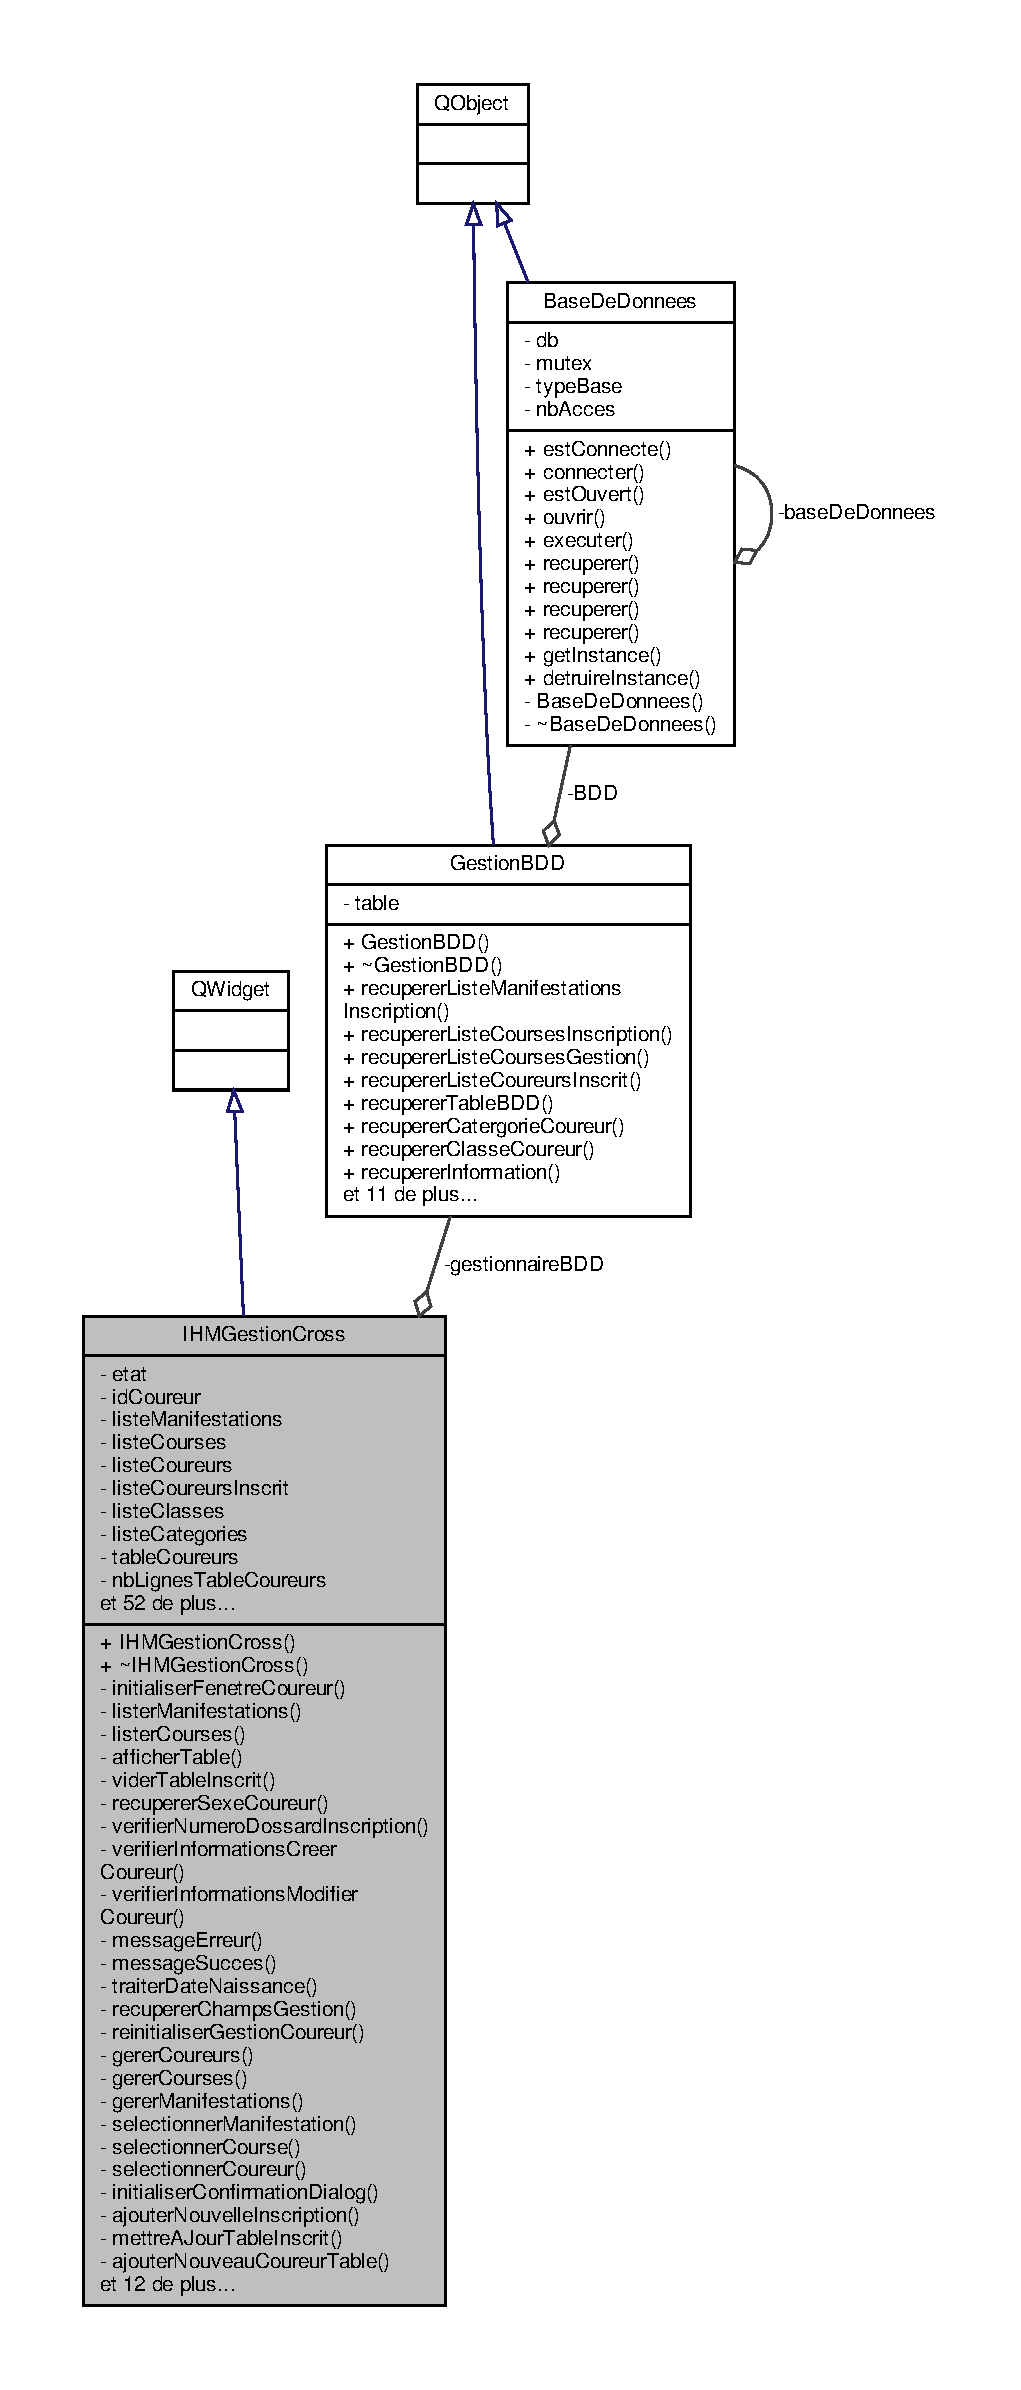
\includegraphics[height=550pt]{class_i_h_m_gestion_cross__coll__graph}
\end{center}
\end{figure}
\subsubsection*{Fonctions membres publiques}
\begin{DoxyCompactItemize}
\item 
\hyperlink{class_i_h_m_gestion_cross_a2c62fd83326a87456a403f46acc408c8}{I\+H\+M\+Gestion\+Cross} (\hyperlink{class_q_widget}{Q\+Widget} $\ast$parent=nullptr)
\begin{DoxyCompactList}\small\item\em Constructeur de la fenêtre principale. \end{DoxyCompactList}\item 
\hyperlink{class_i_h_m_gestion_cross_a47cc1d5e80bea3d5e3396a8c16158c45}{$\sim$\+I\+H\+M\+Gestion\+Cross} ()
\end{DoxyCompactItemize}
\subsubsection*{Connecteurs privés}
\begin{DoxyCompactItemize}
\item 
void \hyperlink{class_i_h_m_gestion_cross_ad46a2295500cf98dbc18f862f6020103}{gerer\+Coureurs} ()
\begin{DoxyCompactList}\small\item\em S\+L\+OT \hyperlink{class_i_h_m_gestion_cross_ad46a2295500cf98dbc18f862f6020103}{gerer\+Coureurs()} de la classe \hyperlink{class_i_h_m_gestion_cross}{I\+H\+M\+Gestion\+Cross}. \end{DoxyCompactList}\item 
void \hyperlink{class_i_h_m_gestion_cross_a82e3861f4959d3599d1d85ee0b3b8654}{gerer\+Courses} ()
\begin{DoxyCompactList}\small\item\em S\+L\+OT \hyperlink{class_i_h_m_gestion_cross_a82e3861f4959d3599d1d85ee0b3b8654}{gerer\+Courses()} de la classe \hyperlink{class_i_h_m_gestion_cross}{I\+H\+M\+Gestion\+Cross}. \end{DoxyCompactList}\item 
void \hyperlink{class_i_h_m_gestion_cross_a406efb83dac8a8ac5d04e9b8cbeaf316}{gerer\+Manifestations} ()
\begin{DoxyCompactList}\small\item\em S\+L\+OT \hyperlink{class_i_h_m_gestion_cross_a406efb83dac8a8ac5d04e9b8cbeaf316}{gerer\+Manifestations()} de la classe \hyperlink{class_i_h_m_gestion_cross}{I\+H\+M\+Gestion\+Cross}. \end{DoxyCompactList}\item 
void \hyperlink{class_i_h_m_gestion_cross_a60fc58610d01534b3df66ac7dd76b4dc}{selectionner\+Manifestation} (Q\+String nom)
\item 
void \hyperlink{class_i_h_m_gestion_cross_ae555b32462455a2cdaf0f8dc2e016d14}{selectionner\+Course} (Q\+String nom)
\item 
void \hyperlink{class_i_h_m_gestion_cross_ad71963d500fd61995fdae94e833db163}{selectionner\+Coureur} (Q\+Model\+Index index)
\item 
void \hyperlink{class_i_h_m_gestion_cross_aa1c728319c825df582a014fc5bd43ea4}{initialiser\+Confirmation\+Dialog} (Q\+String nom\+Tache)
\item 
void \hyperlink{class_i_h_m_gestion_cross_af0165d32344af78b4edce59f88c90ff6}{ajouter\+Nouvelle\+Inscription} ()
\item 
void \hyperlink{class_i_h_m_gestion_cross_a3c96fb9d92e9392ea83b380c3648bf55}{mettre\+A\+Jour\+Table\+Inscrit} (Q\+String\+List inscription)
\item 
void \hyperlink{class_i_h_m_gestion_cross_aa3e6f06ff2f4e724e2f0688528bcf386}{ajouter\+Nouveau\+Coureur\+Table} (Q\+String\+List information\+Coureur)
\item 
void \hyperlink{class_i_h_m_gestion_cross_af13fabb9831fcd237c9c1e7ee75c47b8}{supprimer\+Coureur\+Table} ()
\item 
void \hyperlink{class_i_h_m_gestion_cross_a3a969f85f31f25ed6df6a75a1cee2de1}{modifier\+Coureur\+Table} ()
\item 
void \hyperlink{class_i_h_m_gestion_cross_a53c84315d723d75ad7b4a7d4c317efc5}{mettre\+A\+Jour\+Table\+Coureur} ()
\item 
void \hyperlink{class_i_h_m_gestion_cross_ac8f336c95a5f0c9eb8a4bc1c4bb83445}{passer\+Mode\+Nouveau\+Coureur} ()
\item 
void \hyperlink{class_i_h_m_gestion_cross_a6000b152ba3febb45d6c409519168ba2}{creer\+Coureur} ()
\item 
void \hyperlink{class_i_h_m_gestion_cross_a4fd00fda0e47366d66d046e344a1617e}{supprimer\+Coureur} ()
\item 
void \hyperlink{class_i_h_m_gestion_cross_a1f41cea488ab477505f9d1792c4c2f36}{modifier\+Coureur} ()
\item 
void \hyperlink{class_i_h_m_gestion_cross_a1d3c7f83d4c960f38b237499d2a89731}{initialiser\+Confirmation\+Dialog} ()
\item 
void \hyperlink{class_i_h_m_gestion_cross_a1bf6838771bef4796def7a5ba58d74b3}{annuler\+Nouveau\+Coureur} ()
\item 
void \hyperlink{class_i_h_m_gestion_cross_a144933ab31ae263be7267b93bfd53a82}{confirmer\+Dialog} ()
\item 
void \hyperlink{class_i_h_m_gestion_cross_a58b19fa84a16060a3dd951abeba2c543}{quitter\+Dialog} ()
\item 
void \hyperlink{class_i_h_m_gestion_cross_a9c24746993f720c1067cfe7396ecd5c4}{quitter} ()
\begin{DoxyCompactList}\small\item\em S\+L\+OT \hyperlink{class_i_h_m_gestion_cross_a9c24746993f720c1067cfe7396ecd5c4}{quitter()} de la classe \hyperlink{class_i_h_m_gestion_cross}{I\+H\+M\+Gestion\+Cross}. \end{DoxyCompactList}\end{DoxyCompactItemize}
\subsubsection*{Fonctions membres privées}
\begin{DoxyCompactItemize}
\item 
void \hyperlink{class_i_h_m_gestion_cross_aa5d9de499a66e52b843c4ef4c6074a60}{initialiser\+Fenetre\+Coureur} ()
\item 
void \hyperlink{class_i_h_m_gestion_cross_a0eadd8592c966c89bf7b5a25a0ae7589}{lister\+Manifestations} ()
\item 
void \hyperlink{class_i_h_m_gestion_cross_a34567afe3e94862ebd9af51528dedb65}{lister\+Courses} (Q\+String id\+Manifestation)
\item 
void \hyperlink{class_i_h_m_gestion_cross_ae1510779a1efa3defecb517467e84f91}{afficher\+Table} (Q\+String nom\+Table)
\begin{DoxyCompactList}\small\item\em Méthode \hyperlink{class_i_h_m_gestion_cross_ae1510779a1efa3defecb517467e84f91}{afficher\+Table()} de la classe \hyperlink{class_i_h_m_gestion_cross}{I\+H\+M\+Gestion\+Cross}. \end{DoxyCompactList}\item 
void \hyperlink{class_i_h_m_gestion_cross_ac1ca02b1cb49d9c2f60785c8bd441d60}{vider\+Table\+Inscrit} ()
\item 
Q\+String \hyperlink{class_i_h_m_gestion_cross_a7e1cdc8b3b01f2f2f666f80bf1cc9f5a}{recuperer\+Sexe\+Coureur} ()
\item 
bool \hyperlink{class_i_h_m_gestion_cross_a164be2d046cf18ee03e3939d03a5580d}{verifier\+Numero\+Dossard\+Inscription} (Q\+String numero\+Dossard)
\item 
bool \hyperlink{class_i_h_m_gestion_cross_ae08eec25f5a6d33bf133b0cee78c7c5c}{verifier\+Informations\+Creer\+Coureur} (Q\+String\+List informations)
\item 
bool \hyperlink{class_i_h_m_gestion_cross_a0e088653019d8adefb371348f272d2e2}{verifier\+Informations\+Modifier\+Coureur} (Q\+String\+List informations)
\item 
void \hyperlink{class_i_h_m_gestion_cross_a92fa6016b00d2d4429c901e77d37bf10}{message\+Erreur} (Q\+String message)
\item 
void \hyperlink{class_i_h_m_gestion_cross_a71412d0c3e1d059a646c755803077a7b}{message\+Succes} (Q\+String message)
\item 
Q\+Vector$<$ int $>$ \hyperlink{class_i_h_m_gestion_cross_a4846dcb0c5f95b2b774ab328654bf716}{traiter\+Date\+Naissance} (Q\+String date\+Naissance)
\item 
Q\+String\+List \hyperlink{class_i_h_m_gestion_cross_a271efe8d31fbe05fccfb2dc81e71971a}{recuperer\+Champs\+Gestion} ()
\item 
void \hyperlink{class_i_h_m_gestion_cross_a85c44933ec0dcbb591e01c832063367e}{reinitialiser\+Gestion\+Coureur} ()
\end{DoxyCompactItemize}
\subsubsection*{Attributs privés}
\begin{DoxyCompactItemize}
\item 
Q\+String \hyperlink{class_i_h_m_gestion_cross_a5da4390d71dbd5d05cff339f93c7c85a}{etat}
\item 
Q\+String \hyperlink{class_i_h_m_gestion_cross_a9352a649126c14e7d0da3694c10c3cef}{id\+Coureur}
\item 
\hyperlink{class_gestion_b_d_d}{Gestion\+B\+DD} $\ast$ \hyperlink{class_i_h_m_gestion_cross_a440bac63a3e51db3e2c08e883f8cafc9}{gestionnaire\+B\+DD}
\item 
Q\+Vector$<$ Q\+String $>$ \hyperlink{class_i_h_m_gestion_cross_ac42ca910fa9802b3f63e3393aaa14e8a}{liste\+Manifestations}
\item 
Q\+Vector$<$ Q\+String $>$ \hyperlink{class_i_h_m_gestion_cross_a66fc14c0ed874e72b6ada34e9b83603a}{liste\+Courses}
\item 
Q\+Vector$<$ Q\+String\+List $>$ \hyperlink{class_i_h_m_gestion_cross_a8b2673ec9996d010d3d45f72770ddd87}{liste\+Coureurs}
\item 
Q\+Vector$<$ Q\+String\+List $>$ \hyperlink{class_i_h_m_gestion_cross_a6b7c699caf9ae80c89f4cf5c58ae93d6}{liste\+Coureurs\+Inscrit}
\item 
Q\+Vector$<$ Q\+String\+List $>$ \hyperlink{class_i_h_m_gestion_cross_ab1d62909817e9828796a8c28da193c38}{liste\+Classes}
\item 
Q\+Vector$<$ Q\+String\+List $>$ \hyperlink{class_i_h_m_gestion_cross_a3b5749783a83acaeb513e4170c97bb0e}{liste\+Categories}
\item 
Q\+Vector$<$ Q\+String\+List $>$ \hyperlink{class_i_h_m_gestion_cross_a9bf93b48403da7bf152f013055152630}{table\+Coureurs}
\item 
int \hyperlink{class_i_h_m_gestion_cross_a0f4f5886077b1c5cbfa9cc0680d0380f}{nb\+Lignes\+Table\+Coureurs}
\item 
int \hyperlink{class_i_h_m_gestion_cross_ad33a263cb137ae991a9be57dacc6760a}{nb\+Lignes\+Table\+Inscrit}
\item 
Q\+String\+List \hyperlink{class_i_h_m_gestion_cross_a94c58ce12155f117e0515ce0fc6503bc}{nom\+Colonnes\+Inscrit}
\item 
Q\+Date \hyperlink{class_i_h_m_gestion_cross_a021706ef369d2bf3b95bcb4a8ecfdbe4}{date\+Default}
\item 
Q\+Stacked\+Widget $\ast$ \hyperlink{class_i_h_m_gestion_cross_a2ae4807c25f35813507ff0a2abb2ffb3}{fenetre\+Gestion\+Cross}
\item 
\hyperlink{class_q_widget}{Q\+Widget} $\ast$ \hyperlink{class_i_h_m_gestion_cross_a0e1ed40bb375744135f70cb22d302b02}{fenetre\+Manifestation}
\item 
\hyperlink{class_q_widget}{Q\+Widget} $\ast$ \hyperlink{class_i_h_m_gestion_cross_a939278dde9c1375400bbdd0b3b2476fc}{fenetre\+Course}
\item 
\hyperlink{class_q_widget}{Q\+Widget} $\ast$ \hyperlink{class_i_h_m_gestion_cross_aa776ee3d04b5e02414e4f97ace344c0c}{fenetre\+Coureur}
\item 
Q\+Push\+Button $\ast$ \hyperlink{class_i_h_m_gestion_cross_a540b4525e546b6d61988245ae53768ce}{b\+Manifestations}
\item 
Q\+Push\+Button $\ast$ \hyperlink{class_i_h_m_gestion_cross_a0df377aec07ada51a115cc458854c966}{b\+Courses}
\item 
Q\+Push\+Button $\ast$ \hyperlink{class_i_h_m_gestion_cross_ac2819198bae00b7e0f23e8bc491b4cbb}{b\+Coureurs}
\item 
Q\+Label $\ast$ \hyperlink{class_i_h_m_gestion_cross_abfb2504c2d5189d08e24677e04ddf3ba}{label\+Gestion}
\item 
Q\+Label $\ast$ \hyperlink{class_i_h_m_gestion_cross_a58c321e2d95796d99e70a05260b8aff3}{label\+Inscription}
\item 
Q\+Label $\ast$ \hyperlink{class_i_h_m_gestion_cross_a2025ba71cf1bdbfbec56a8f5552d7a83}{logo\+Chrono\+Cross}
\item 
Q\+Label $\ast$ \hyperlink{class_i_h_m_gestion_cross_a866a6f0ba317b299d4aede5fc276b2bb}{label\+Gestion\+Nom}
\item 
Q\+Label $\ast$ \hyperlink{class_i_h_m_gestion_cross_ae213fa44e6e291f9ca02d8b091ab0d06}{label\+Gestion\+Prenom}
\item 
Q\+Label $\ast$ \hyperlink{class_i_h_m_gestion_cross_af15625b1b1bfb04468f0ed7c6ba39b1b}{label\+Gestion\+Date\+Naissance}
\item 
Q\+Label $\ast$ \hyperlink{class_i_h_m_gestion_cross_a4f070ed70d6d076d07c96562e366c805}{label\+Gestion\+Classe}
\item 
Q\+Label $\ast$ \hyperlink{class_i_h_m_gestion_cross_a04af17f1ebbbbac6d9c4509c94bc6f39}{label\+Gestion\+Categorie}
\item 
Q\+Label $\ast$ \hyperlink{class_i_h_m_gestion_cross_a56e8930b11c38475450df50a48d4581e}{label\+Gestion\+I\+NE}
\item 
Q\+Label $\ast$ \hyperlink{class_i_h_m_gestion_cross_a2e720e692a029a3f4f516a9ad00d2731}{label\+Gestion\+Sexe}
\item 
Q\+Label $\ast$ \hyperlink{class_i_h_m_gestion_cross_a0106cdcaf86997642d48dfad96a2368f}{label\+Gestion\+Participe}
\item 
Q\+Push\+Button $\ast$ \hyperlink{class_i_h_m_gestion_cross_ab987235a79961d3d186878052a02b21b}{b\+Gestion\+Nouveau}
\item 
Q\+Push\+Button $\ast$ \hyperlink{class_i_h_m_gestion_cross_aac8a7363e20bc9ba2f65b7d9b3bc856e}{b\+Creation\+Confirmer}
\item 
Q\+Push\+Button $\ast$ \hyperlink{class_i_h_m_gestion_cross_a297a77054dc0f54e461c0f9b0382efb3}{b\+Creation\+Annuler}
\item 
Q\+Push\+Button $\ast$ \hyperlink{class_i_h_m_gestion_cross_a524ced9992dcc4e7ee25b01e30c4c5df}{b\+Gestion\+Modifier}
\item 
Q\+Push\+Button $\ast$ \hyperlink{class_i_h_m_gestion_cross_adc5bed6caf7f597dd30999bc871e695b}{b\+Gestion\+Supprimer}
\item 
Q\+Push\+Button $\ast$ \hyperlink{class_i_h_m_gestion_cross_a1afbc04ebd42deafebbbdc998d0fc246}{b\+Inscrire}
\item 
Q\+Date\+Edit $\ast$ \hyperlink{class_i_h_m_gestion_cross_a1c63c5c91be88aef13d2582e48dff7d0}{de\+Date\+Naissance}
\item 
Q\+Line\+Edit $\ast$ \hyperlink{class_i_h_m_gestion_cross_a633102626c5dedd575b51a1ba5c6e708}{line\+Edit\+Nom}
\item 
Q\+Line\+Edit $\ast$ \hyperlink{class_i_h_m_gestion_cross_a7bea7529f01cf8ca8f365d418aae52d5}{line\+Edit\+Prenom}
\item 
Q\+Combo\+Box $\ast$ \hyperlink{class_i_h_m_gestion_cross_af734c4b13942dd83fbbd0355e3728c9f}{cb\+Gestion\+Classe}
\item 
Q\+Combo\+Box $\ast$ \hyperlink{class_i_h_m_gestion_cross_a60cdc44c61bcd4e1e189c8de5556b89e}{cb\+Gestion\+Categorie}
\item 
Q\+Combo\+Box $\ast$ \hyperlink{class_i_h_m_gestion_cross_a89aff3b1c5d5198dd7aaecd932331e0d}{cb\+Gestion\+Participe}
\item 
Q\+Line\+Edit $\ast$ \hyperlink{class_i_h_m_gestion_cross_ab6c32fd079f81c4fa0b9ec0b4ef9bb61}{line\+Edit\+I\+NE}
\item 
Q\+Radio\+Button $\ast$ \hyperlink{class_i_h_m_gestion_cross_a4474ef47310eb3511befdf1beaa18b56}{rb\+Gestion\+SexeF}
\item 
Q\+Radio\+Button $\ast$ \hyperlink{class_i_h_m_gestion_cross_a7d471a7f96862dcd302f7f8cc52dfea4}{rb\+Gestion\+SexeM}
\item 
Q\+Label $\ast$ \hyperlink{class_i_h_m_gestion_cross_affb681e48eb407d5d69d1ecb24da8377}{label\+Inscription\+Manifestation}
\item 
Q\+Combo\+Box $\ast$ \hyperlink{class_i_h_m_gestion_cross_a317ffd7cc1c9aa5d6e55c53568e44f98}{cb\+Inscription\+Liste\+Manifestation}
\item 
Q\+Label $\ast$ \hyperlink{class_i_h_m_gestion_cross_a88b058cc1d4031891e26eb62409af6bb}{label\+Inscription\+Course}
\item 
Q\+Combo\+Box $\ast$ \hyperlink{class_i_h_m_gestion_cross_aff44e6f1a225ee5b55783afe72049f83}{cb\+Inscription\+Liste\+Course}
\item 
Q\+Label $\ast$ \hyperlink{class_i_h_m_gestion_cross_a3209e0dfc51bb3a17e2ef700a778178b}{label\+Numero\+Dossard}
\item 
Q\+Line\+Edit $\ast$ \hyperlink{class_i_h_m_gestion_cross_adeb4cfc9a218c06fca5cabc280a611e2}{line\+Edit\+Numero\+Dossard}
\item 
Q\+Table\+View $\ast$ \hyperlink{class_i_h_m_gestion_cross_a4a0ba98c5b671a38d67942254d2329db}{vue\+Table\+Coureurs}
\item 
Q\+Standard\+Item\+Model $\ast$ \hyperlink{class_i_h_m_gestion_cross_ad9560c4804694dbbf969de5f6f56eb30}{modele\+Table\+Coureurs}
\item 
Q\+String\+List \hyperlink{class_i_h_m_gestion_cross_ab95ce87fd2f9427023040cc8d0077681}{nom\+Colonnes\+Coureur}
\item 
Q\+Table\+View $\ast$ \hyperlink{class_i_h_m_gestion_cross_a79b4e49cf8b22c9894d366e08b722c55}{vue\+Table\+Inscrits}
\item 
Q\+Standard\+Item\+Model $\ast$ \hyperlink{class_i_h_m_gestion_cross_a19565551280115e642ceb9790c7317bc}{modele\+Table\+Inscrits}
\item 
Q\+Label $\ast$ \hyperlink{class_i_h_m_gestion_cross_a1855bd63290c39c20660064b41710e8c}{label\+Message\+Inscription}
\item 
Q\+Dialog $\ast$ \hyperlink{class_i_h_m_gestion_cross_a417b63ff11c3be6623d17718d9058768}{confirmation\+Dialog}
\item 
Q\+Label $\ast$ \hyperlink{class_i_h_m_gestion_cross_a9b51d06493979981248ecc2641f82be4}{label\+Confirmation\+Dialog}
\item 
Q\+Push\+Button $\ast$ \hyperlink{class_i_h_m_gestion_cross_a8aaf51ea455654df21f65ed496384b60}{b\+Confirmation\+Dialog}
\item 
Q\+Push\+Button $\ast$ \hyperlink{class_i_h_m_gestion_cross_a2efd604a10cae21b2f85e7196c3927fd}{b\+Annuler\+Dialog}
\end{DoxyCompactItemize}


\subsubsection{Description détaillée}
La fenêtre principale de l\textquotesingle{}application Gestion-\/\+Cross. 

\begin{DoxyAuthor}{Auteur}
A\+N\+D\+R\+EO Michaël 
\end{DoxyAuthor}
\begin{DoxyVersion}{Version}
1.\+0 
\end{DoxyVersion}


\subsubsection{Documentation des constructeurs et destructeur}
\mbox{\Hypertarget{class_i_h_m_gestion_cross_a2c62fd83326a87456a403f46acc408c8}\label{class_i_h_m_gestion_cross_a2c62fd83326a87456a403f46acc408c8}} 
\index{I\+H\+M\+Gestion\+Cross@{I\+H\+M\+Gestion\+Cross}!I\+H\+M\+Gestion\+Cross@{I\+H\+M\+Gestion\+Cross}}
\index{I\+H\+M\+Gestion\+Cross@{I\+H\+M\+Gestion\+Cross}!I\+H\+M\+Gestion\+Cross@{I\+H\+M\+Gestion\+Cross}}
\paragraph{\texorpdfstring{I\+H\+M\+Gestion\+Cross()}{IHMGestionCross()}}
{\footnotesize\ttfamily I\+H\+M\+Gestion\+Cross\+::\+I\+H\+M\+Gestion\+Cross (\begin{DoxyParamCaption}\item[{\hyperlink{class_q_widget}{Q\+Widget} $\ast$}]{parent = {\ttfamily nullptr} }\end{DoxyParamCaption})}



Constructeur de la fenêtre principale. 


\begin{DoxyParams}{Paramètres}
{\em parent} & \\
\hline
\end{DoxyParams}


Références \hyperlink{class_i_h_m_gestion_cross_aa3e6f06ff2f4e724e2f0688528bcf386}{ajouter\+Nouveau\+Coureur\+Table()}, \hyperlink{class_i_h_m_gestion_cross_af0165d32344af78b4edce59f88c90ff6}{ajouter\+Nouvelle\+Inscription()}, \hyperlink{class_i_h_m_gestion_cross_a1bf6838771bef4796def7a5ba58d74b3}{annuler\+Nouveau\+Coureur()}, \hyperlink{class_i_h_m_gestion_cross_ac2819198bae00b7e0f23e8bc491b4cbb}{b\+Coureurs}, \hyperlink{class_i_h_m_gestion_cross_a0df377aec07ada51a115cc458854c966}{b\+Courses}, \hyperlink{class_i_h_m_gestion_cross_a297a77054dc0f54e461c0f9b0382efb3}{b\+Creation\+Annuler}, \hyperlink{class_i_h_m_gestion_cross_aac8a7363e20bc9ba2f65b7d9b3bc856e}{b\+Creation\+Confirmer}, \hyperlink{class_i_h_m_gestion_cross_a524ced9992dcc4e7ee25b01e30c4c5df}{b\+Gestion\+Modifier}, \hyperlink{class_i_h_m_gestion_cross_ab987235a79961d3d186878052a02b21b}{b\+Gestion\+Nouveau}, \hyperlink{class_i_h_m_gestion_cross_adc5bed6caf7f597dd30999bc871e695b}{b\+Gestion\+Supprimer}, \hyperlink{class_i_h_m_gestion_cross_a1afbc04ebd42deafebbbdc998d0fc246}{b\+Inscrire}, \hyperlink{class_i_h_m_gestion_cross_a540b4525e546b6d61988245ae53768ce}{b\+Manifestations}, \hyperlink{class_i_h_m_gestion_cross_aff44e6f1a225ee5b55783afe72049f83}{cb\+Inscription\+Liste\+Course}, \hyperlink{class_i_h_m_gestion_cross_a317ffd7cc1c9aa5d6e55c53568e44f98}{cb\+Inscription\+Liste\+Manifestation}, \hyperlink{class_i_h_m_gestion_cross_a6000b152ba3febb45d6c409519168ba2}{creer\+Coureur()}, \hyperlink{class_i_h_m_gestion_cross_a021706ef369d2bf3b95bcb4a8ecfdbe4}{date\+Default}, \hyperlink{class_i_h_m_gestion_cross_aa776ee3d04b5e02414e4f97ace344c0c}{fenetre\+Coureur}, \hyperlink{class_i_h_m_gestion_cross_a939278dde9c1375400bbdd0b3b2476fc}{fenetre\+Course}, \hyperlink{class_i_h_m_gestion_cross_a2ae4807c25f35813507ff0a2abb2ffb3}{fenetre\+Gestion\+Cross}, \hyperlink{class_i_h_m_gestion_cross_a0e1ed40bb375744135f70cb22d302b02}{fenetre\+Manifestation}, \hyperlink{class_i_h_m_gestion_cross_ad46a2295500cf98dbc18f862f6020103}{gerer\+Coureurs()}, \hyperlink{class_i_h_m_gestion_cross_a82e3861f4959d3599d1d85ee0b3b8654}{gerer\+Courses()}, \hyperlink{class_i_h_m_gestion_cross_a406efb83dac8a8ac5d04e9b8cbeaf316}{gerer\+Manifestations()}, \hyperlink{class_i_h_m_gestion_cross_a440bac63a3e51db3e2c08e883f8cafc9}{gestionnaire\+B\+DD}, \hyperlink{ihmchronocross_8h_aa8bee638aa78f9b332485225ecc8e75e}{I\+M\+A\+G\+E\+C\+H\+R\+O\+N\+O\+C\+R\+O\+SS}, \hyperlink{class_i_h_m_gestion_cross_aa5d9de499a66e52b843c4ef4c6074a60}{initialiser\+Fenetre\+Coureur()}, \hyperlink{class_i_h_m_gestion_cross_a2025ba71cf1bdbfbec56a8f5552d7a83}{logo\+Chrono\+Cross}, \hyperlink{class_i_h_m_gestion_cross_a3c96fb9d92e9392ea83b380c3648bf55}{mettre\+A\+Jour\+Table\+Inscrit()}, \hyperlink{class_i_h_m_gestion_cross_a1f41cea488ab477505f9d1792c4c2f36}{modifier\+Coureur()}, \hyperlink{class_i_h_m_gestion_cross_a3a969f85f31f25ed6df6a75a1cee2de1}{modifier\+Coureur\+Table()}, \hyperlink{class_i_h_m_gestion_cross_a0f4f5886077b1c5cbfa9cc0680d0380f}{nb\+Lignes\+Table\+Coureurs}, \hyperlink{class_i_h_m_gestion_cross_ac8f336c95a5f0c9eb8a4bc1c4bb83445}{passer\+Mode\+Nouveau\+Coureur()}, \hyperlink{class_i_h_m_gestion_cross_a9c24746993f720c1067cfe7396ecd5c4}{quitter()}, \hyperlink{class_i_h_m_gestion_cross_ad71963d500fd61995fdae94e833db163}{selectionner\+Coureur()}, \hyperlink{class_i_h_m_gestion_cross_ae555b32462455a2cdaf0f8dc2e016d14}{selectionner\+Course()}, \hyperlink{class_i_h_m_gestion_cross_a60fc58610d01534b3df66ac7dd76b4dc}{selectionner\+Manifestation()}, \hyperlink{class_i_h_m_gestion_cross_a4fd00fda0e47366d66d046e344a1617e}{supprimer\+Coureur()}, \hyperlink{class_i_h_m_gestion_cross_af13fabb9831fcd237c9c1e7ee75c47b8}{supprimer\+Coureur\+Table()}, \hyperlink{ihmgestioncross_8h_a562719681712f3dd8e5b5a158597e78b}{T\+A\+I\+L\+L\+E\+T\+E\+X\+T\+E\+B\+O\+U\+T\+O\+N\+T\+I\+T\+RE}, et \hyperlink{class_i_h_m_gestion_cross_a4a0ba98c5b671a38d67942254d2329db}{vue\+Table\+Coureurs}.


\begin{DoxyCode}
00015                                                 : \hyperlink{class_q_widget}{QWidget}(parent)
00016 \{
00017     qDebug() << Q\_FUNC\_INFO;
00018 
00019     \hyperlink{class_i_h_m_gestion_cross_a440bac63a3e51db3e2c08e883f8cafc9}{gestionnaireBDD} = \textcolor{keyword}{new} \hyperlink{class_gestion_b_d_d}{GestionBDD}(\textcolor{keyword}{this});
00020     \hyperlink{class_i_h_m_gestion_cross_a0f4f5886077b1c5cbfa9cc0680d0380f}{nbLignesTableCoureurs} = 0;
00021     QVector<int> valeurDateDefault;
00022     valeurDateDefault << 2000 << 01 << 01;
00023     \hyperlink{class_i_h_m_gestion_cross_a021706ef369d2bf3b95bcb4a8ecfdbe4}{dateDefault}.setDate(valeurDateDefault[0], valeurDateDefault[1], valeurDateDefault[2]);
00024     qDebug() << Q\_FUNC\_INFO << \hyperlink{class_i_h_m_gestion_cross_a021706ef369d2bf3b95bcb4a8ecfdbe4}{dateDefault};
00025 
00026     setStyleSheet(QLatin1String(\textcolor{stringliteral}{"QWidget\(\backslash\)n"}
00027     \textcolor{stringliteral}{"\{\(\backslash\)n"}
00028     \textcolor{stringliteral}{"   background-color: white;\(\backslash\)n"}
00029     \textcolor{stringliteral}{"\}\(\backslash\)n"}
00030     \textcolor{stringliteral}{"QPushButton \{\(\backslash\)n"}
00031     \textcolor{stringliteral}{"    background-color: lightgray;\(\backslash\)n"}
00032     \textcolor{stringliteral}{"    border-width: 1px;\(\backslash\)n"}
00033     \textcolor{stringliteral}{"    border-color: black;\(\backslash\)n"}
00034     \textcolor{stringliteral}{"    border-style: solid;\(\backslash\)n"}
00035     \textcolor{stringliteral}{"    border-radius: 1;\(\backslash\)n"}
00036     \textcolor{stringliteral}{"    padding: 5px;\(\backslash\)n"}
00037     \textcolor{stringliteral}{"    min-width: 9ex;\(\backslash\)n"}
00038     \textcolor{stringliteral}{"    min-height: 2.5ex;\(\backslash\)n"}
00039     \textcolor{stringliteral}{"\}\(\backslash\)n"}
00040     \textcolor{stringliteral}{"\(\backslash\)n"}
00041     \textcolor{stringliteral}{"QPushButton:hover:enabled \{\(\backslash\)n"}
00042     \textcolor{stringliteral}{"   background-color: gray;\(\backslash\)n"}
00043     \textcolor{stringliteral}{"\}\(\backslash\)n"}
00044     \textcolor{stringliteral}{"\(\backslash\)n"}
00045     \textcolor{stringliteral}{"QPushButton:pressed \{\(\backslash\)n"}
00046     \textcolor{stringliteral}{"    padding-left: 5px;\(\backslash\)n"}
00047     \textcolor{stringliteral}{"    padding-top: 5px;\(\backslash\)n"}
00048     \textcolor{stringliteral}{"    background-color: white;\(\backslash\)n"}
00049     \textcolor{stringliteral}{"\}\(\backslash\)n"}
00050     \textcolor{stringliteral}{"\(\backslash\)n"}
00051     \textcolor{stringliteral}{"QPushButton:checked \{\(\backslash\)n"}
00052     \textcolor{stringliteral}{"background-color: white;\(\backslash\)n"}
00053     \textcolor{stringliteral}{"\}\(\backslash\)n"}
00054     \textcolor{stringliteral}{"QComboBox, QLineEdit \{\(\backslash\)n"}
00055     \textcolor{stringliteral}{"    background-color: white;\(\backslash\)n"}
00056     \textcolor{stringliteral}{"    selection-color: #0a214c; \(\backslash\)n"}
00057     \textcolor{stringliteral}{"    selection-background-color: white;\(\backslash\)n"}
00058     \textcolor{stringliteral}{"    border-width: 1px;\(\backslash\)n"}
00059     \textcolor{stringliteral}{"    padding: 3px;\(\backslash\)n"}
00060     \textcolor{stringliteral}{"    border-style: solid;\(\backslash\)n"}
00061     \textcolor{stringliteral}{"    border-color: gray;\(\backslash\)n"}
00062     \textcolor{stringliteral}{"    border-radius: 5px;\(\backslash\)n"}
00063     \textcolor{stringliteral}{"\}\(\backslash\)n"}
00064     \textcolor{stringliteral}{"\(\backslash\)n"}
00065     \textcolor{stringliteral}{"QLineEdit:focus \{\(\backslash\)n"}
00066     \textcolor{stringliteral}{"    border-width: 2px;\(\backslash\)n"}
00067     \textcolor{stringliteral}{"    padding: 0px;\(\backslash\)n"}
00068     \textcolor{stringliteral}{"\}\(\backslash\)n"}
00069     \textcolor{stringliteral}{"\(\backslash\)n"}
00070     \textcolor{stringliteral}{"QComboBox::item:hover \{\(\backslash\)n"}
00071     \textcolor{stringliteral}{"    background-color: white;\(\backslash\)n"}
00072     \textcolor{stringliteral}{"\}\(\backslash\)n"}
00073     \textcolor{stringliteral}{""}));
00074 
00075     QFont texteButton;
00076     texteButton.setPointSize(\hyperlink{ihmgestioncross_8h_a562719681712f3dd8e5b5a158597e78b}{TAILLETEXTEBOUTONTITRE});
00077 
00078     \hyperlink{class_i_h_m_gestion_cross_a2ae4807c25f35813507ff0a2abb2ffb3}{fenetreGestionCross} = \textcolor{keyword}{new} QStackedWidget(\textcolor{keyword}{this});
00079     \hyperlink{class_i_h_m_gestion_cross_a0e1ed40bb375744135f70cb22d302b02}{fenetreManifestation} = \textcolor{keyword}{new} \hyperlink{class_q_widget}{QWidget}(\textcolor{keyword}{this});
00080     \hyperlink{class_i_h_m_gestion_cross_a939278dde9c1375400bbdd0b3b2476fc}{fenetreCourse} = \textcolor{keyword}{new} \hyperlink{class_q_widget}{QWidget}(\textcolor{keyword}{this});
00081     \hyperlink{class_i_h_m_gestion_cross_aa776ee3d04b5e02414e4f97ace344c0c}{fenetreCoureur} = \textcolor{keyword}{new} \hyperlink{class_q_widget}{QWidget}(\textcolor{keyword}{this});
00082 
00083     \hyperlink{class_i_h_m_gestion_cross_a2ae4807c25f35813507ff0a2abb2ffb3}{fenetreGestionCross}->addWidget(\hyperlink{class_i_h_m_gestion_cross_a0e1ed40bb375744135f70cb22d302b02}{fenetreManifestation});
00084     \hyperlink{class_i_h_m_gestion_cross_a2ae4807c25f35813507ff0a2abb2ffb3}{fenetreGestionCross}->addWidget(\hyperlink{class_i_h_m_gestion_cross_a939278dde9c1375400bbdd0b3b2476fc}{fenetreCourse});
00085     \hyperlink{class_i_h_m_gestion_cross_a2ae4807c25f35813507ff0a2abb2ffb3}{fenetreGestionCross}->addWidget(\hyperlink{class_i_h_m_gestion_cross_aa776ee3d04b5e02414e4f97ace344c0c}{fenetreCoureur});
00086 
00087     \hyperlink{class_i_h_m_gestion_cross_aa5d9de499a66e52b843c4ef4c6074a60}{initialiserFenetreCoureur}();
00088 
00089     \hyperlink{class_i_h_m_gestion_cross_a540b4525e546b6d61988245ae53768ce}{bManifestations} = \textcolor{keyword}{new} QPushButton(QString::fromUtf8(\textcolor{stringliteral}{"Manifestations"}), \textcolor{keyword}{this});
00090     \hyperlink{class_i_h_m_gestion_cross_a540b4525e546b6d61988245ae53768ce}{bManifestations}->setCheckable(\textcolor{keyword}{true});
00091     \hyperlink{class_i_h_m_gestion_cross_a540b4525e546b6d61988245ae53768ce}{bManifestations}->setFont(texteButton);
00092 
00093     \hyperlink{class_i_h_m_gestion_cross_a0df377aec07ada51a115cc458854c966}{bCourses} = \textcolor{keyword}{new} QPushButton(QString::fromUtf8(\textcolor{stringliteral}{"Courses"}), \textcolor{keyword}{this});
00094     \hyperlink{class_i_h_m_gestion_cross_a0df377aec07ada51a115cc458854c966}{bCourses}->setCheckable(\textcolor{keyword}{true});
00095     \hyperlink{class_i_h_m_gestion_cross_a0df377aec07ada51a115cc458854c966}{bCourses}->setFont(texteButton);
00096 
00097     \hyperlink{class_i_h_m_gestion_cross_ac2819198bae00b7e0f23e8bc491b4cbb}{bCoureurs} = \textcolor{keyword}{new} QPushButton(QString::fromUtf8(\textcolor{stringliteral}{"Coureurs"}), \textcolor{keyword}{this});
00098     \hyperlink{class_i_h_m_gestion_cross_ac2819198bae00b7e0f23e8bc491b4cbb}{bCoureurs}->setCheckable(\textcolor{keyword}{true});
00099     \hyperlink{class_i_h_m_gestion_cross_ac2819198bae00b7e0f23e8bc491b4cbb}{bCoureurs}->setFont(texteButton);
00100 
00101     \hyperlink{class_i_h_m_gestion_cross_a2025ba71cf1bdbfbec56a8f5552d7a83}{logoChronoCross} = \textcolor{keyword}{new} QLabel(\textcolor{keyword}{this});
00102     QPixmap pixmap\_img(\hyperlink{ihmchronocross_8h_aa8bee638aa78f9b332485225ecc8e75e}{IMAGECHRONOCROSS});
00103     \hyperlink{class_i_h_m_gestion_cross_a2025ba71cf1bdbfbec56a8f5552d7a83}{logoChronoCross}->setPixmap(pixmap\_img);
00104 
00105     QHBoxLayout *hBoutons = \textcolor{keyword}{new} QHBoxLayout;
00106     QHBoxLayout *hLayoutFenetre = \textcolor{keyword}{new} QHBoxLayout;
00107     QVBoxLayout *mainLayout = \textcolor{keyword}{new} QVBoxLayout;
00108 
00109     hBoutons->addWidget(\hyperlink{class_i_h_m_gestion_cross_a540b4525e546b6d61988245ae53768ce}{bManifestations});
00110     hBoutons->addWidget(\hyperlink{class_i_h_m_gestion_cross_a0df377aec07ada51a115cc458854c966}{bCourses});
00111     hBoutons->addWidget(\hyperlink{class_i_h_m_gestion_cross_ac2819198bae00b7e0f23e8bc491b4cbb}{bCoureurs});
00112     hBoutons->addStretch();
00113     hBoutons->addWidget(\hyperlink{class_i_h_m_gestion_cross_a2025ba71cf1bdbfbec56a8f5552d7a83}{logoChronoCross});
00114     hBoutons->setContentsMargins(0, 0, 0, 40); \textcolor{comment}{// G H D B}
00115     hLayoutFenetre->addWidget(\hyperlink{class_i_h_m_gestion_cross_a2ae4807c25f35813507ff0a2abb2ffb3}{fenetreGestionCross});
00116     mainLayout->addLayout(hBoutons);
00117     mainLayout->addLayout(hLayoutFenetre);
00118 
00119     setLayout(mainLayout);
00120     setWindowTitle(\textcolor{stringliteral}{"Gestion-Cross"});
00121     setContextMenuPolicy(Qt::ActionsContextMenu);
00122 
00123     QAction *actionQuitter = \textcolor{keyword}{new} QAction(\textcolor{stringliteral}{"&Quitter"}, \textcolor{keyword}{this});
00124     actionQuitter->setShortcut(QKeySequence::Quit);
00125     addAction(actionQuitter);
00126 
00127     QAction *actionEntrerPAD = \textcolor{keyword}{new} QAction(\textcolor{stringliteral}{"&Entrer1"}, \textcolor{keyword}{this});
00128     actionEntrerPAD->setShortcut(QKeySequence(Qt::Key\_Enter));
00129     addAction(actionEntrerPAD);
00130 
00131     QAction *actionEntrerRETURN = \textcolor{keyword}{new} QAction(\textcolor{stringliteral}{"&Entrer2"}, \textcolor{keyword}{this});
00132     actionEntrerRETURN->setShortcut(QKeySequence(Qt::Key\_Return));
00133     addAction(actionEntrerRETURN);
00134 
00135     \textcolor{comment}{//Connect}
00136     connect(actionQuitter, SIGNAL(triggered()), \textcolor{keyword}{this}, SLOT(\hyperlink{class_i_h_m_gestion_cross_a9c24746993f720c1067cfe7396ecd5c4}{quitter}()));
00137     connect(actionEntrerPAD, SIGNAL(triggered()), \textcolor{keyword}{this}, SLOT(
      \hyperlink{class_i_h_m_gestion_cross_af0165d32344af78b4edce59f88c90ff6}{ajouterNouvelleInscription}()));
00138     connect(actionEntrerRETURN, SIGNAL(triggered()), \textcolor{keyword}{this}, SLOT(
      \hyperlink{class_i_h_m_gestion_cross_af0165d32344af78b4edce59f88c90ff6}{ajouterNouvelleInscription}()));
00139 
00140     connect(\hyperlink{class_i_h_m_gestion_cross_ac2819198bae00b7e0f23e8bc491b4cbb}{bCoureurs}, SIGNAL(clicked()), \textcolor{keyword}{this}, SLOT(\hyperlink{class_i_h_m_gestion_cross_ad46a2295500cf98dbc18f862f6020103}{gererCoureurs}()));
00141     connect(\hyperlink{class_i_h_m_gestion_cross_a0df377aec07ada51a115cc458854c966}{bCourses}, SIGNAL(clicked()), \textcolor{keyword}{this}, SLOT(\hyperlink{class_i_h_m_gestion_cross_a82e3861f4959d3599d1d85ee0b3b8654}{gererCourses}()));
00142     connect(\hyperlink{class_i_h_m_gestion_cross_a540b4525e546b6d61988245ae53768ce}{bManifestations}, SIGNAL(clicked()), \textcolor{keyword}{this}, SLOT(
      \hyperlink{class_i_h_m_gestion_cross_a406efb83dac8a8ac5d04e9b8cbeaf316}{gererManifestations}()));
00143     connect(\hyperlink{class_i_h_m_gestion_cross_a1afbc04ebd42deafebbbdc998d0fc246}{bInscrire}, SIGNAL(clicked()), \textcolor{keyword}{this}, SLOT(
      \hyperlink{class_i_h_m_gestion_cross_af0165d32344af78b4edce59f88c90ff6}{ajouterNouvelleInscription}()));
00144     connect(\hyperlink{class_i_h_m_gestion_cross_ab987235a79961d3d186878052a02b21b}{bGestionNouveau}, SIGNAL(clicked()), \textcolor{keyword}{this}, SLOT(
      \hyperlink{class_i_h_m_gestion_cross_ac8f336c95a5f0c9eb8a4bc1c4bb83445}{passerModeNouveauCoureur}()));
00145     connect(\hyperlink{class_i_h_m_gestion_cross_aac8a7363e20bc9ba2f65b7d9b3bc856e}{bCreationConfirmer}, SIGNAL(clicked()), \textcolor{keyword}{this}, SLOT(
      \hyperlink{class_i_h_m_gestion_cross_a6000b152ba3febb45d6c409519168ba2}{creerCoureur}()));
00146     connect(\hyperlink{class_i_h_m_gestion_cross_a297a77054dc0f54e461c0f9b0382efb3}{bCreationAnnuler}, SIGNAL(clicked()), \textcolor{keyword}{this}, SLOT(
      \hyperlink{class_i_h_m_gestion_cross_a1bf6838771bef4796def7a5ba58d74b3}{annulerNouveauCoureur}()));
00147     connect(\hyperlink{class_i_h_m_gestion_cross_adc5bed6caf7f597dd30999bc871e695b}{bGestionSupprimer}, SIGNAL(clicked()), \textcolor{keyword}{this}, SLOT(
      \hyperlink{class_i_h_m_gestion_cross_a4fd00fda0e47366d66d046e344a1617e}{supprimerCoureur}()));
00148     connect(\hyperlink{class_i_h_m_gestion_cross_a524ced9992dcc4e7ee25b01e30c4c5df}{bGestionModifier}, SIGNAL(clicked()), \textcolor{keyword}{this}, SLOT(
      \hyperlink{class_i_h_m_gestion_cross_a1f41cea488ab477505f9d1792c4c2f36}{modifierCoureur}()));
00149 
00150     connect(\hyperlink{class_i_h_m_gestion_cross_a4a0ba98c5b671a38d67942254d2329db}{vueTableCoureurs}, SIGNAL(clicked(QModelIndex)), \textcolor{keyword}{this}, SLOT(
      \hyperlink{class_i_h_m_gestion_cross_ad71963d500fd61995fdae94e833db163}{selectionnerCoureur}(QModelIndex)));
00151     connect(\hyperlink{class_i_h_m_gestion_cross_a317ffd7cc1c9aa5d6e55c53568e44f98}{cbInscriptionListeManifestation}, SIGNAL(currentIndexChanged(
      QString)), \textcolor{keyword}{this}, SLOT(\hyperlink{class_i_h_m_gestion_cross_a60fc58610d01534b3df66ac7dd76b4dc}{selectionnerManifestation}(QString)));
00152     connect(\hyperlink{class_i_h_m_gestion_cross_aff44e6f1a225ee5b55783afe72049f83}{cbInscriptionListeCourse}, SIGNAL(currentIndexChanged(QString)), \textcolor{keyword}{this}, 
      SLOT(\hyperlink{class_i_h_m_gestion_cross_ae555b32462455a2cdaf0f8dc2e016d14}{selectionnerCourse}(QString)));
00153     connect(\hyperlink{class_i_h_m_gestion_cross_a440bac63a3e51db3e2c08e883f8cafc9}{gestionnaireBDD}, SIGNAL(nouvelInscrit(QStringList)), \textcolor{keyword}{this}, SLOT(
      \hyperlink{class_i_h_m_gestion_cross_a3c96fb9d92e9392ea83b380c3648bf55}{mettreAJourTableInscrit}(QStringList)));
00154     connect(\hyperlink{class_i_h_m_gestion_cross_a440bac63a3e51db3e2c08e883f8cafc9}{gestionnaireBDD}, SIGNAL(nouveauCoureur(QStringList)), \textcolor{keyword}{this}, SLOT(
      \hyperlink{class_i_h_m_gestion_cross_aa3e6f06ff2f4e724e2f0688528bcf386}{ajouterNouveauCoureurTable}(QStringList)));
00155     connect(\hyperlink{class_i_h_m_gestion_cross_a440bac63a3e51db3e2c08e883f8cafc9}{gestionnaireBDD}, SIGNAL(coureurSupprime()), \textcolor{keyword}{this}, SLOT(
      \hyperlink{class_i_h_m_gestion_cross_af13fabb9831fcd237c9c1e7ee75c47b8}{supprimerCoureurTable}()));
00156     connect(\hyperlink{class_i_h_m_gestion_cross_a440bac63a3e51db3e2c08e883f8cafc9}{gestionnaireBDD}, SIGNAL(coureurModifie()), \textcolor{keyword}{this}, SLOT(
      \hyperlink{class_i_h_m_gestion_cross_a3a969f85f31f25ed6df6a75a1cee2de1}{modifierCoureurTable}()));
00157 
00158     setWindowFlags(Qt::Window | Qt::WindowCloseButtonHint);
00159     showMaximized();
00160 
00161     \hyperlink{class_i_h_m_gestion_cross_ad46a2295500cf98dbc18f862f6020103}{gererCoureurs}();
00162 \}
\end{DoxyCode}
\mbox{\Hypertarget{class_i_h_m_gestion_cross_a47cc1d5e80bea3d5e3396a8c16158c45}\label{class_i_h_m_gestion_cross_a47cc1d5e80bea3d5e3396a8c16158c45}} 
\index{I\+H\+M\+Gestion\+Cross@{I\+H\+M\+Gestion\+Cross}!````~I\+H\+M\+Gestion\+Cross@{$\sim$\+I\+H\+M\+Gestion\+Cross}}
\index{````~I\+H\+M\+Gestion\+Cross@{$\sim$\+I\+H\+M\+Gestion\+Cross}!I\+H\+M\+Gestion\+Cross@{I\+H\+M\+Gestion\+Cross}}
\paragraph{\texorpdfstring{$\sim$\+I\+H\+M\+Gestion\+Cross()}{~IHMGestionCross()}}
{\footnotesize\ttfamily I\+H\+M\+Gestion\+Cross\+::$\sim$\+I\+H\+M\+Gestion\+Cross (\begin{DoxyParamCaption}{ }\end{DoxyParamCaption})}



Références \hyperlink{class_base_de_donnees_a457401c0816b888c77ce915997545f4e}{Base\+De\+Donnees\+::detruire\+Instance()}.


\begin{DoxyCode}
00165 \{
00166     \hyperlink{class_base_de_donnees_a457401c0816b888c77ce915997545f4e}{BaseDeDonnees::detruireInstance}();
00167     qDebug() << Q\_FUNC\_INFO;
00168 \}
\end{DoxyCode}


\subsubsection{Documentation des fonctions membres}
\mbox{\Hypertarget{class_i_h_m_gestion_cross_ae1510779a1efa3defecb517467e84f91}\label{class_i_h_m_gestion_cross_ae1510779a1efa3defecb517467e84f91}} 
\index{I\+H\+M\+Gestion\+Cross@{I\+H\+M\+Gestion\+Cross}!afficher\+Table@{afficher\+Table}}
\index{afficher\+Table@{afficher\+Table}!I\+H\+M\+Gestion\+Cross@{I\+H\+M\+Gestion\+Cross}}
\paragraph{\texorpdfstring{afficher\+Table()}{afficherTable()}}
{\footnotesize\ttfamily void I\+H\+M\+Gestion\+Cross\+::afficher\+Table (\begin{DoxyParamCaption}\item[{Q\+String}]{nom\+Table }\end{DoxyParamCaption})\hspace{0.3cm}{\ttfamily [private]}}



Méthode \hyperlink{class_i_h_m_gestion_cross_ae1510779a1efa3defecb517467e84f91}{afficher\+Table()} de la classe \hyperlink{class_i_h_m_gestion_cross}{I\+H\+M\+Gestion\+Cross}. 

Récupère la table \hyperlink{class_coureur}{Coureur} de la base de données et l\textquotesingle{}affiche dans le tableau 
\begin{DoxyParams}{Paramètres}
{\em nom\+Table} & Q\+String \\
\hline
\end{DoxyParams}


Références \hyperlink{ihmgestioncross_8h_a24ffa4392b8af69a94a6500ec4a60a7e}{C\+O\+L\+O\+N\+N\+E\+\_\+\+C\+A\+T\+E\+G\+O\+R\+IE}, \hyperlink{ihmchronocross_8h_a114680edc01528f77bb689b0a2ca18a2}{C\+O\+L\+O\+N\+N\+E\+\_\+\+C\+L\+A\+S\+SE}, \hyperlink{ihmgestioncross_8h_a985c9028f6a7ed4b42d0e93eeef6c28c}{C\+O\+L\+O\+N\+N\+E\+\_\+\+D\+A\+T\+E\+N\+A\+I\+S\+S\+A\+N\+CE}, \hyperlink{ihmgestioncross_8h_aa8208c9f9fd2ea2418e4b7bb28175f80}{C\+O\+L\+O\+N\+N\+E\+\_\+\+I\+NE}, \hyperlink{ihmchronocross_8h_aeee76385895c145ef5a633e6c6812603}{C\+O\+L\+O\+N\+N\+E\+\_\+\+N\+OM}, \hyperlink{ihmchronocross_8h_a5d6f240d26209cd66db8aa5e1aac62f9}{C\+O\+L\+O\+N\+N\+E\+\_\+\+P\+R\+E\+N\+OM}, \hyperlink{ihmgestioncross_8h_a9ef0920ad9f4f65e80e5d9f8e1b263b2}{C\+O\+L\+O\+N\+N\+E\+\_\+\+S\+E\+XE}, \hyperlink{class_i_h_m_gestion_cross_a440bac63a3e51db3e2c08e883f8cafc9}{gestionnaire\+B\+DD}, \hyperlink{ihmgestioncross_8h_aadb5aa9454077354c643312a81834cf6}{I\+N\+F\+O\+\_\+\+C\+O\+U\+R\+E\+U\+R\+\_\+\+C\+A\+T\+E\+G\+O\+R\+IE}, \hyperlink{ihmchronocross_8h_a104dfa4cfc656a690caaec36fd4d3e2d}{I\+N\+F\+O\+\_\+\+C\+O\+U\+R\+E\+U\+R\+\_\+\+C\+L\+A\+S\+SE}, \hyperlink{ihmgestioncross_8h_a887f2ea4595905eedb8c2580dad1c276}{I\+N\+F\+O\+\_\+\+C\+O\+U\+R\+E\+U\+R\+\_\+\+D\+A\+T\+E\+N\+A\+I\+S\+S\+A\+N\+CE}, \hyperlink{ihmgestioncross_8h_a2e5435ad2b0c61674b2dad6c0ea46301}{I\+N\+F\+O\+\_\+\+C\+O\+U\+R\+E\+U\+R\+\_\+\+I\+NE}, \hyperlink{ihmchronocross_8h_a71b99ea06ae916bcd158edbd441c8c24}{I\+N\+F\+O\+\_\+\+C\+O\+U\+R\+E\+U\+R\+\_\+\+N\+OM}, \hyperlink{ihmchronocross_8h_a68fd2611ad0ef66da1a71726675067e7}{I\+N\+F\+O\+\_\+\+C\+O\+U\+R\+E\+U\+R\+\_\+\+P\+R\+E\+N\+OM}, \hyperlink{ihmgestioncross_8h_a3f85ead669b0bcc0b9bf09a92a8dd933}{I\+N\+F\+O\+\_\+\+C\+O\+U\+R\+E\+U\+R\+\_\+\+S\+E\+XE}, \hyperlink{class_i_h_m_gestion_cross_ad9560c4804694dbbf969de5f6f56eb30}{modele\+Table\+Coureurs}, \hyperlink{class_i_h_m_gestion_cross_a0f4f5886077b1c5cbfa9cc0680d0380f}{nb\+Lignes\+Table\+Coureurs}, \hyperlink{class_gestion_b_d_d_a0a2fa02b90974684658937fbfb55bf0a}{Gestion\+B\+D\+D\+::recuperer\+Information()}, \hyperlink{class_gestion_b_d_d_a2b44ebc5bf5b1a7babde6512817a85b4}{Gestion\+B\+D\+D\+::recuperer\+Table\+B\+D\+D()}, et \hyperlink{class_i_h_m_gestion_cross_a9bf93b48403da7bf152f013055152630}{table\+Coureurs}.



Référencé par \hyperlink{class_i_h_m_gestion_cross_ad46a2295500cf98dbc18f862f6020103}{gerer\+Coureurs()}, \hyperlink{class_i_h_m_gestion_cross_a3a969f85f31f25ed6df6a75a1cee2de1}{modifier\+Coureur\+Table()}, et \hyperlink{class_i_h_m_gestion_cross_af13fabb9831fcd237c9c1e7ee75c47b8}{supprimer\+Coureur\+Table()}.


\begin{DoxyCode}
00457 \{
00458     \textcolor{comment}{// enregistrement [ idCoureur, idCatégorie, idClasse, INE, Nom, Prenom, DateNaissance, Sexe ]}
00459     \textcolor{comment}{// tableau [ nom prenom classe categorie INE datenaissace sexe ]}
00460     \hyperlink{class_i_h_m_gestion_cross_a9bf93b48403da7bf152f013055152630}{tableCoureurs}.clear();
00461     \hyperlink{class_i_h_m_gestion_cross_a9bf93b48403da7bf152f013055152630}{tableCoureurs} = \hyperlink{class_i_h_m_gestion_cross_a440bac63a3e51db3e2c08e883f8cafc9}{gestionnaireBDD}->
      \hyperlink{class_gestion_b_d_d_a2b44ebc5bf5b1a7babde6512817a85b4}{recupererTableBDD}(nomTable);
00462     \textcolor{keywordflow}{if}(\hyperlink{class_i_h_m_gestion_cross_a9bf93b48403da7bf152f013055152630}{tableCoureurs}.size() == 0)
00463         \textcolor{keywordflow}{return};
00464     QStringList enregistrement;
00465     \textcolor{keywordtype}{int} nbEnregistrements = \hyperlink{class_i_h_m_gestion_cross_a9bf93b48403da7bf152f013055152630}{tableCoureurs}.count();
00466 
00467     qDebug() << Q\_FUNC\_INFO << nbEnregistrements;
00468 
00469     \textcolor{keywordflow}{for}(\textcolor{keywordtype}{int} i = 0; i < nbEnregistrements; i += 1)
00470     \{
00471         enregistrement = \hyperlink{class_i_h_m_gestion_cross_a9bf93b48403da7bf152f013055152630}{tableCoureurs}[i];
00472         QStandardItem *nom = \textcolor{keyword}{new} QStandardItem(enregistrement.at(
      \hyperlink{ihmchronocross_8h_a71b99ea06ae916bcd158edbd441c8c24}{INFO\_COUREUR\_NOM}));
00473         QStandardItem *prenom = \textcolor{keyword}{new} QStandardItem(enregistrement.at(
      \hyperlink{ihmchronocross_8h_a68fd2611ad0ef66da1a71726675067e7}{INFO\_COUREUR\_PRENOM}));
00474         QStandardItem *classe = \textcolor{keyword}{new} QStandardItem(\hyperlink{class_i_h_m_gestion_cross_a440bac63a3e51db3e2c08e883f8cafc9}{gestionnaireBDD}->
      \hyperlink{class_gestion_b_d_d_a0a2fa02b90974684658937fbfb55bf0a}{recupererInformation}(\textcolor{stringliteral}{"Nom"}, \textcolor{stringliteral}{"Classe"}, QString(\textcolor{stringliteral}{"idClasse = %1;"}).arg(enregistrement[
      \hyperlink{ihmchronocross_8h_a104dfa4cfc656a690caaec36fd4d3e2d}{INFO\_COUREUR\_CLASSE}])));
00475 
00476         QStandardItem *categorie = \textcolor{keyword}{new} QStandardItem(\hyperlink{class_i_h_m_gestion_cross_a440bac63a3e51db3e2c08e883f8cafc9}{gestionnaireBDD}->
      \hyperlink{class_gestion_b_d_d_a0a2fa02b90974684658937fbfb55bf0a}{recupererInformation}(\textcolor{stringliteral}{"Nom"}, \textcolor{stringliteral}{"Categorie"}, QString(\textcolor{stringliteral}{"idCategorie = %1;"}).arg(
      enregistrement[\hyperlink{ihmgestioncross_8h_aadb5aa9454077354c643312a81834cf6}{INFO\_COUREUR\_CATEGORIE}])));
00477         QStandardItem *ine = \textcolor{keyword}{new} QStandardItem(enregistrement.at(
      \hyperlink{ihmgestioncross_8h_a2e5435ad2b0c61674b2dad6c0ea46301}{INFO\_COUREUR\_INE}));
00478         QStandardItem *dateNaissance = \textcolor{keyword}{new} QStandardItem(enregistrement.at(
      \hyperlink{ihmgestioncross_8h_a887f2ea4595905eedb8c2580dad1c276}{INFO\_COUREUR\_DATENAISSANCE}));
00479         QStandardItem *sexe = \textcolor{keyword}{new} QStandardItem(enregistrement.at(
      \hyperlink{ihmgestioncross_8h_a3f85ead669b0bcc0b9bf09a92a8dd933}{INFO\_COUREUR\_SEXE}));
00480 
00481         \hyperlink{class_i_h_m_gestion_cross_ad9560c4804694dbbf969de5f6f56eb30}{modeleTableCoureurs}->setItem(i, \hyperlink{ihmchronocross_8h_aeee76385895c145ef5a633e6c6812603}{COLONNE\_NOM}, nom);
00482         \hyperlink{class_i_h_m_gestion_cross_ad9560c4804694dbbf969de5f6f56eb30}{modeleTableCoureurs}->setItem(i, \hyperlink{ihmchronocross_8h_a5d6f240d26209cd66db8aa5e1aac62f9}{COLONNE\_PRENOM}, prenom);
00483         \hyperlink{class_i_h_m_gestion_cross_ad9560c4804694dbbf969de5f6f56eb30}{modeleTableCoureurs}->setItem(i, \hyperlink{ihmchronocross_8h_a114680edc01528f77bb689b0a2ca18a2}{COLONNE\_CLASSE}, classe);
00484         \hyperlink{class_i_h_m_gestion_cross_ad9560c4804694dbbf969de5f6f56eb30}{modeleTableCoureurs}->setItem(i, \hyperlink{ihmgestioncross_8h_a24ffa4392b8af69a94a6500ec4a60a7e}{COLONNE\_CATEGORIE}, categorie);
00485         \hyperlink{class_i_h_m_gestion_cross_ad9560c4804694dbbf969de5f6f56eb30}{modeleTableCoureurs}->setItem(i, \hyperlink{ihmgestioncross_8h_aa8208c9f9fd2ea2418e4b7bb28175f80}{COLONNE\_INE}, ine);
00486         \hyperlink{class_i_h_m_gestion_cross_ad9560c4804694dbbf969de5f6f56eb30}{modeleTableCoureurs}->setItem(i, \hyperlink{ihmgestioncross_8h_a985c9028f6a7ed4b42d0e93eeef6c28c}{COLONNE\_DATENAISSANCE}, 
      dateNaissance);
00487         \hyperlink{class_i_h_m_gestion_cross_ad9560c4804694dbbf969de5f6f56eb30}{modeleTableCoureurs}->setItem(i, \hyperlink{ihmgestioncross_8h_a9ef0920ad9f4f65e80e5d9f8e1b263b2}{COLONNE\_SEXE}, sexe);
00488 
00489         enregistrement.clear();
00490     \}
00491     \hyperlink{class_i_h_m_gestion_cross_a0f4f5886077b1c5cbfa9cc0680d0380f}{nbLignesTableCoureurs} = \hyperlink{class_i_h_m_gestion_cross_ad9560c4804694dbbf969de5f6f56eb30}{modeleTableCoureurs}->rowCount();
00492 \}
\end{DoxyCode}
\mbox{\Hypertarget{class_i_h_m_gestion_cross_aa3e6f06ff2f4e724e2f0688528bcf386}\label{class_i_h_m_gestion_cross_aa3e6f06ff2f4e724e2f0688528bcf386}} 
\index{I\+H\+M\+Gestion\+Cross@{I\+H\+M\+Gestion\+Cross}!ajouter\+Nouveau\+Coureur\+Table@{ajouter\+Nouveau\+Coureur\+Table}}
\index{ajouter\+Nouveau\+Coureur\+Table@{ajouter\+Nouveau\+Coureur\+Table}!I\+H\+M\+Gestion\+Cross@{I\+H\+M\+Gestion\+Cross}}
\paragraph{\texorpdfstring{ajouter\+Nouveau\+Coureur\+Table}{ajouterNouveauCoureurTable}}
{\footnotesize\ttfamily void I\+H\+M\+Gestion\+Cross\+::ajouter\+Nouveau\+Coureur\+Table (\begin{DoxyParamCaption}\item[{Q\+String\+List}]{information\+Coureur }\end{DoxyParamCaption})\hspace{0.3cm}{\ttfamily [private]}, {\ttfamily [slot]}}



Références \hyperlink{ihmgestioncross_8h_a24ffa4392b8af69a94a6500ec4a60a7e}{C\+O\+L\+O\+N\+N\+E\+\_\+\+C\+A\+T\+E\+G\+O\+R\+IE}, \hyperlink{ihmchronocross_8h_a114680edc01528f77bb689b0a2ca18a2}{C\+O\+L\+O\+N\+N\+E\+\_\+\+C\+L\+A\+S\+SE}, \hyperlink{ihmgestioncross_8h_a985c9028f6a7ed4b42d0e93eeef6c28c}{C\+O\+L\+O\+N\+N\+E\+\_\+\+D\+A\+T\+E\+N\+A\+I\+S\+S\+A\+N\+CE}, \hyperlink{ihmgestioncross_8h_aa8208c9f9fd2ea2418e4b7bb28175f80}{C\+O\+L\+O\+N\+N\+E\+\_\+\+I\+NE}, \hyperlink{ihmchronocross_8h_aeee76385895c145ef5a633e6c6812603}{C\+O\+L\+O\+N\+N\+E\+\_\+\+N\+OM}, \hyperlink{ihmchronocross_8h_a5d6f240d26209cd66db8aa5e1aac62f9}{C\+O\+L\+O\+N\+N\+E\+\_\+\+P\+R\+E\+N\+OM}, \hyperlink{ihmgestioncross_8h_a9ef0920ad9f4f65e80e5d9f8e1b263b2}{C\+O\+L\+O\+N\+N\+E\+\_\+\+S\+E\+XE}, \hyperlink{class_i_h_m_gestion_cross_a71412d0c3e1d059a646c755803077a7b}{message\+Succes()}, \hyperlink{class_i_h_m_gestion_cross_a53c84315d723d75ad7b4a7d4c317efc5}{mettre\+A\+Jour\+Table\+Coureur()}, \hyperlink{class_i_h_m_gestion_cross_ad9560c4804694dbbf969de5f6f56eb30}{modele\+Table\+Coureurs}, et \hyperlink{class_i_h_m_gestion_cross_a0f4f5886077b1c5cbfa9cc0680d0380f}{nb\+Lignes\+Table\+Coureurs}.



Référencé par \hyperlink{class_i_h_m_gestion_cross_a2c62fd83326a87456a403f46acc408c8}{I\+H\+M\+Gestion\+Cross()}.


\begin{DoxyCode}
01012 \{
01013     qDebug() << Q\_FUNC\_INFO << informationsCoureur;
01014     \textcolor{comment}{// informationsCoureur [ 0 categorie , 1 classe , 2 ine , 3 nom , 4 prenom , 5 datenaissance , 6 sexe ]}
01015     \textcolor{keywordflow}{if}(\hyperlink{class_i_h_m_gestion_cross_a0f4f5886077b1c5cbfa9cc0680d0380f}{nbLignesTableCoureurs} != \hyperlink{class_i_h_m_gestion_cross_ad9560c4804694dbbf969de5f6f56eb30}{modeleTableCoureurs}->rowCount())
01016         \hyperlink{class_i_h_m_gestion_cross_a0f4f5886077b1c5cbfa9cc0680d0380f}{nbLignesTableCoureurs} = \hyperlink{class_i_h_m_gestion_cross_ad9560c4804694dbbf969de5f6f56eb30}{modeleTableCoureurs}->rowCount();
01017     \hyperlink{class_i_h_m_gestion_cross_ad9560c4804694dbbf969de5f6f56eb30}{modeleTableCoureurs}->insertRow(\hyperlink{class_i_h_m_gestion_cross_a0f4f5886077b1c5cbfa9cc0680d0380f}{nbLignesTableCoureurs});
01018 
01019     \hyperlink{class_i_h_m_gestion_cross_a71412d0c3e1d059a646c755803077a7b}{messageSucces}(\textcolor{stringliteral}{"créé(e)"});
01020 
01021     QStandardItem *categorie = \textcolor{keyword}{new} QStandardItem(informationsCoureur.at(0));
01022     QStandardItem *classe  = \textcolor{keyword}{new} QStandardItem(informationsCoureur.at(1));
01023     QStandardItem *ine  = \textcolor{keyword}{new} QStandardItem(informationsCoureur.at(2));
01024     QStandardItem *nom  = \textcolor{keyword}{new} QStandardItem(informationsCoureur.at(3));
01025     QStandardItem *prenom  = \textcolor{keyword}{new} QStandardItem(informationsCoureur.at(4));
01026     QStandardItem *dateNaissance  = \textcolor{keyword}{new} QStandardItem(informationsCoureur.at(5));
01027     QStandardItem *sexe  = \textcolor{keyword}{new} QStandardItem(informationsCoureur.at(6));
01028 
01029     \hyperlink{class_i_h_m_gestion_cross_ad9560c4804694dbbf969de5f6f56eb30}{modeleTableCoureurs}->setItem(\hyperlink{class_i_h_m_gestion_cross_a0f4f5886077b1c5cbfa9cc0680d0380f}{nbLignesTableCoureurs}, 
      \hyperlink{ihmchronocross_8h_aeee76385895c145ef5a633e6c6812603}{COLONNE\_NOM}, nom);
01030     \hyperlink{class_i_h_m_gestion_cross_ad9560c4804694dbbf969de5f6f56eb30}{modeleTableCoureurs}->setItem(\hyperlink{class_i_h_m_gestion_cross_a0f4f5886077b1c5cbfa9cc0680d0380f}{nbLignesTableCoureurs}, 
      \hyperlink{ihmchronocross_8h_a5d6f240d26209cd66db8aa5e1aac62f9}{COLONNE\_PRENOM}, prenom);
01031     \hyperlink{class_i_h_m_gestion_cross_ad9560c4804694dbbf969de5f6f56eb30}{modeleTableCoureurs}->setItem(\hyperlink{class_i_h_m_gestion_cross_a0f4f5886077b1c5cbfa9cc0680d0380f}{nbLignesTableCoureurs}, 
      \hyperlink{ihmchronocross_8h_a114680edc01528f77bb689b0a2ca18a2}{COLONNE\_CLASSE}, classe);
01032     \hyperlink{class_i_h_m_gestion_cross_ad9560c4804694dbbf969de5f6f56eb30}{modeleTableCoureurs}->setItem(\hyperlink{class_i_h_m_gestion_cross_a0f4f5886077b1c5cbfa9cc0680d0380f}{nbLignesTableCoureurs}, 
      \hyperlink{ihmgestioncross_8h_a24ffa4392b8af69a94a6500ec4a60a7e}{COLONNE\_CATEGORIE}, categorie);
01033     \hyperlink{class_i_h_m_gestion_cross_ad9560c4804694dbbf969de5f6f56eb30}{modeleTableCoureurs}->setItem(\hyperlink{class_i_h_m_gestion_cross_a0f4f5886077b1c5cbfa9cc0680d0380f}{nbLignesTableCoureurs}, 
      \hyperlink{ihmgestioncross_8h_aa8208c9f9fd2ea2418e4b7bb28175f80}{COLONNE\_INE}, ine);
01034     \hyperlink{class_i_h_m_gestion_cross_ad9560c4804694dbbf969de5f6f56eb30}{modeleTableCoureurs}->setItem(\hyperlink{class_i_h_m_gestion_cross_a0f4f5886077b1c5cbfa9cc0680d0380f}{nbLignesTableCoureurs}, 
      \hyperlink{ihmgestioncross_8h_a985c9028f6a7ed4b42d0e93eeef6c28c}{COLONNE\_DATENAISSANCE}, dateNaissance);
01035     \hyperlink{class_i_h_m_gestion_cross_ad9560c4804694dbbf969de5f6f56eb30}{modeleTableCoureurs}->setItem(\hyperlink{class_i_h_m_gestion_cross_a0f4f5886077b1c5cbfa9cc0680d0380f}{nbLignesTableCoureurs}, 
      \hyperlink{ihmgestioncross_8h_a9ef0920ad9f4f65e80e5d9f8e1b263b2}{COLONNE\_SEXE}, sexe);
01036 
01037     \hyperlink{class_i_h_m_gestion_cross_ad9560c4804694dbbf969de5f6f56eb30}{modeleTableCoureurs}->sort(4,Qt::SortOrder::AscendingOrder);
01038     \hyperlink{class_i_h_m_gestion_cross_a53c84315d723d75ad7b4a7d4c317efc5}{mettreAJourTableCoureur}();
01039 
01040 \}
\end{DoxyCode}
\mbox{\Hypertarget{class_i_h_m_gestion_cross_af0165d32344af78b4edce59f88c90ff6}\label{class_i_h_m_gestion_cross_af0165d32344af78b4edce59f88c90ff6}} 
\index{I\+H\+M\+Gestion\+Cross@{I\+H\+M\+Gestion\+Cross}!ajouter\+Nouvelle\+Inscription@{ajouter\+Nouvelle\+Inscription}}
\index{ajouter\+Nouvelle\+Inscription@{ajouter\+Nouvelle\+Inscription}!I\+H\+M\+Gestion\+Cross@{I\+H\+M\+Gestion\+Cross}}
\paragraph{\texorpdfstring{ajouter\+Nouvelle\+Inscription}{ajouterNouvelleInscription}}
{\footnotesize\ttfamily void I\+H\+M\+Gestion\+Cross\+::ajouter\+Nouvelle\+Inscription (\begin{DoxyParamCaption}{ }\end{DoxyParamCaption})\hspace{0.3cm}{\ttfamily [private]}, {\ttfamily [slot]}}



Références \hyperlink{class_gestion_b_d_d_a71391d5419969b52cd999463b5326599}{Gestion\+B\+D\+D\+::ajouter\+Nouvel\+Inscrit()}, \hyperlink{class_i_h_m_gestion_cross_aff44e6f1a225ee5b55783afe72049f83}{cb\+Inscription\+Liste\+Course}, \hyperlink{class_i_h_m_gestion_cross_a440bac63a3e51db3e2c08e883f8cafc9}{gestionnaire\+B\+DD}, \hyperlink{class_i_h_m_gestion_cross_a9352a649126c14e7d0da3694c10c3cef}{id\+Coureur}, \hyperlink{class_i_h_m_gestion_cross_a633102626c5dedd575b51a1ba5c6e708}{line\+Edit\+Nom}, \hyperlink{class_i_h_m_gestion_cross_adeb4cfc9a218c06fca5cabc280a611e2}{line\+Edit\+Numero\+Dossard}, \hyperlink{class_i_h_m_gestion_cross_a0eadd8592c966c89bf7b5a25a0ae7589}{lister\+Manifestations()}, \hyperlink{class_gestion_b_d_d_a0a2fa02b90974684658937fbfb55bf0a}{Gestion\+B\+D\+D\+::recuperer\+Information()}, et \hyperlink{class_i_h_m_gestion_cross_a164be2d046cf18ee03e3939d03a5580d}{verifier\+Numero\+Dossard\+Inscription()}.



Référencé par \hyperlink{class_i_h_m_gestion_cross_a2c62fd83326a87456a403f46acc408c8}{I\+H\+M\+Gestion\+Cross()}.


\begin{DoxyCode}
00977 \{
00978 
00979     QString numeroDossard = \hyperlink{class_i_h_m_gestion_cross_adeb4cfc9a218c06fca5cabc280a611e2}{lineEditNumeroDossard}->text();
00980     \textcolor{keywordflow}{if}(\hyperlink{class_i_h_m_gestion_cross_a164be2d046cf18ee03e3939d03a5580d}{verifierNumeroDossardInscription}(numeroDossard))
00981     \{
00982         qDebug() << Q\_FUNC\_INFO << \textcolor{stringliteral}{"Dossad valide"};
00983         QStringList inscription;
00984         QString nomCourse = \hyperlink{class_i_h_m_gestion_cross_aff44e6f1a225ee5b55783afe72049f83}{cbInscriptionListeCourse}->currentText();
00985         QString idCourse = \hyperlink{class_i_h_m_gestion_cross_a440bac63a3e51db3e2c08e883f8cafc9}{gestionnaireBDD}->\hyperlink{class_gestion_b_d_d_a0a2fa02b90974684658937fbfb55bf0a}{recupererInformation}(\textcolor{stringliteral}{"
      idCourse"}, \textcolor{stringliteral}{"Course"}, QString(\textcolor{stringliteral}{"Nom = '%1'"}).arg(nomCourse));
00986         QString \hyperlink{class_i_h_m_gestion_cross_a9352a649126c14e7d0da3694c10c3cef}{idCoureur} = \hyperlink{class_i_h_m_gestion_cross_a440bac63a3e51db3e2c08e883f8cafc9}{gestionnaireBDD}->
      \hyperlink{class_gestion_b_d_d_a0a2fa02b90974684658937fbfb55bf0a}{recupererInformation}(\textcolor{stringliteral}{"idCoureur"}, \textcolor{stringliteral}{"Coureur"}, QString(\textcolor{stringliteral}{"Nom = '%1'"}).arg(
      \hyperlink{class_i_h_m_gestion_cross_a633102626c5dedd575b51a1ba5c6e708}{lineEditNom}->text()));
00987         qDebug() << Q\_FUNC\_INFO << \textcolor{stringliteral}{"Inscription :\(\backslash\)tidCoureur : "} << idCoureur << \textcolor{stringliteral}{"\(\backslash\)tidCourse : "} << 
      idCourse << \textcolor{stringliteral}{"\(\backslash\)tnumero : "} << numeroDossard;
00988         inscription << idCoureur << idCourse << numeroDossard;
00989         \hyperlink{class_i_h_m_gestion_cross_a440bac63a3e51db3e2c08e883f8cafc9}{gestionnaireBDD}->\hyperlink{class_gestion_b_d_d_a71391d5419969b52cd999463b5326599}{ajouterNouvelInscrit}(inscription);
00990         \hyperlink{class_i_h_m_gestion_cross_adeb4cfc9a218c06fca5cabc280a611e2}{lineEditNumeroDossard}->clear();
00991         \hyperlink{class_i_h_m_gestion_cross_a0eadd8592c966c89bf7b5a25a0ae7589}{listerManifestations}();
00992     \}
00993     \textcolor{keywordflow}{else}
00994         qDebug() << Q\_FUNC\_INFO << \textcolor{stringliteral}{"Dossard invalide"};
00995 \}
\end{DoxyCode}
\mbox{\Hypertarget{class_i_h_m_gestion_cross_a1bf6838771bef4796def7a5ba58d74b3}\label{class_i_h_m_gestion_cross_a1bf6838771bef4796def7a5ba58d74b3}} 
\index{I\+H\+M\+Gestion\+Cross@{I\+H\+M\+Gestion\+Cross}!annuler\+Nouveau\+Coureur@{annuler\+Nouveau\+Coureur}}
\index{annuler\+Nouveau\+Coureur@{annuler\+Nouveau\+Coureur}!I\+H\+M\+Gestion\+Cross@{I\+H\+M\+Gestion\+Cross}}
\paragraph{\texorpdfstring{annuler\+Nouveau\+Coureur}{annulerNouveauCoureur}}
{\footnotesize\ttfamily void I\+H\+M\+Gestion\+Cross\+::annuler\+Nouveau\+Coureur (\begin{DoxyParamCaption}{ }\end{DoxyParamCaption})\hspace{0.3cm}{\ttfamily [private]}, {\ttfamily [slot]}}



Références \hyperlink{class_i_h_m_gestion_cross_a85c44933ec0dcbb591e01c832063367e}{reinitialiser\+Gestion\+Coureur()}.



Référencé par \hyperlink{class_i_h_m_gestion_cross_a2c62fd83326a87456a403f46acc408c8}{I\+H\+M\+Gestion\+Cross()}.


\begin{DoxyCode}
01128 \{
01129     \hyperlink{class_i_h_m_gestion_cross_a85c44933ec0dcbb591e01c832063367e}{reinitialiserGestionCoureur}();
01130 \}
\end{DoxyCode}
\mbox{\Hypertarget{class_i_h_m_gestion_cross_a144933ab31ae263be7267b93bfd53a82}\label{class_i_h_m_gestion_cross_a144933ab31ae263be7267b93bfd53a82}} 
\index{I\+H\+M\+Gestion\+Cross@{I\+H\+M\+Gestion\+Cross}!confirmer\+Dialog@{confirmer\+Dialog}}
\index{confirmer\+Dialog@{confirmer\+Dialog}!I\+H\+M\+Gestion\+Cross@{I\+H\+M\+Gestion\+Cross}}
\paragraph{\texorpdfstring{confirmer\+Dialog}{confirmerDialog}}
{\footnotesize\ttfamily void I\+H\+M\+Gestion\+Cross\+::confirmer\+Dialog (\begin{DoxyParamCaption}{ }\end{DoxyParamCaption})\hspace{0.3cm}{\ttfamily [private]}, {\ttfamily [slot]}}



Références \hyperlink{class_i_h_m_gestion_cross_a417b63ff11c3be6623d17718d9058768}{confirmation\+Dialog}, \hyperlink{class_i_h_m_gestion_cross_a5da4390d71dbd5d05cff339f93c7c85a}{etat}, \hyperlink{class_i_h_m_gestion_cross_a440bac63a3e51db3e2c08e883f8cafc9}{gestionnaire\+B\+DD}, \hyperlink{class_i_h_m_gestion_cross_a9352a649126c14e7d0da3694c10c3cef}{id\+Coureur}, \hyperlink{class_i_h_m_gestion_cross_ab6c32fd079f81c4fa0b9ec0b4ef9bb61}{line\+Edit\+I\+NE}, \hyperlink{class_gestion_b_d_d_afad096d7e405d35a818d4858ee34df61}{Gestion\+B\+D\+D\+::modifier\+Coureur()}, \hyperlink{class_i_h_m_gestion_cross_a271efe8d31fbe05fccfb2dc81e71971a}{recuperer\+Champs\+Gestion()}, \hyperlink{class_gestion_b_d_d_afe47ec92274b7998131c5d4e6551d177}{Gestion\+B\+D\+D\+::supprimer\+Coureur()}, et \hyperlink{class_i_h_m_gestion_cross_a0e088653019d8adefb371348f272d2e2}{verifier\+Informations\+Modifier\+Coureur()}.



Référencé par \hyperlink{class_i_h_m_gestion_cross_a1d3c7f83d4c960f38b237499d2a89731}{initialiser\+Confirmation\+Dialog()}.


\begin{DoxyCode}
01177 \{
01178     \textcolor{keywordflow}{if}(\hyperlink{class_i_h_m_gestion_cross_a5da4390d71dbd5d05cff339f93c7c85a}{etat} == \textcolor{stringliteral}{"Suppression Coureur"})
01179     \{
01180         QString INE = \hyperlink{class_i_h_m_gestion_cross_ab6c32fd079f81c4fa0b9ec0b4ef9bb61}{lineEditINE}->text();
01181         qDebug() << Q\_FUNC\_INFO << \textcolor{stringliteral}{"SUPPRESSION DEMANDÉ"} << INE;
01182         \hyperlink{class_i_h_m_gestion_cross_a440bac63a3e51db3e2c08e883f8cafc9}{gestionnaireBDD}->\hyperlink{class_gestion_b_d_d_afe47ec92274b7998131c5d4e6551d177}{supprimerCoureur}(INE);
01183     \}
01184     \textcolor{keywordflow}{else} \textcolor{keywordflow}{if}(\hyperlink{class_i_h_m_gestion_cross_a5da4390d71dbd5d05cff339f93c7c85a}{etat} == \textcolor{stringliteral}{"Modification Coureur"})
01185     \{
01186         QStringList informationsCoureur = \hyperlink{class_i_h_m_gestion_cross_a271efe8d31fbe05fccfb2dc81e71971a}{recupererChampsGestion}();
01187         informationsCoureur << \hyperlink{class_i_h_m_gestion_cross_a9352a649126c14e7d0da3694c10c3cef}{idCoureur};
01188         \textcolor{keywordflow}{if}(\hyperlink{class_i_h_m_gestion_cross_a0e088653019d8adefb371348f272d2e2}{verifierInformationsModifierCoureur}(informationsCoureur))
01189         \{
01190             informationsCoureur << \hyperlink{class_i_h_m_gestion_cross_a9352a649126c14e7d0da3694c10c3cef}{idCoureur};
01191             qDebug() << Q\_FUNC\_INFO << \textcolor{stringliteral}{"MODIFICATION DEMANDÉ"};
01192             \hyperlink{class_i_h_m_gestion_cross_a440bac63a3e51db3e2c08e883f8cafc9}{gestionnaireBDD}->\hyperlink{class_gestion_b_d_d_afad096d7e405d35a818d4858ee34df61}{modifierCoureur}(informationsCoureur);
01193         \}
01194     \}
01195     \hyperlink{class_i_h_m_gestion_cross_a417b63ff11c3be6623d17718d9058768}{confirmationDialog}->close();
01196 \}
\end{DoxyCode}
\mbox{\Hypertarget{class_i_h_m_gestion_cross_a6000b152ba3febb45d6c409519168ba2}\label{class_i_h_m_gestion_cross_a6000b152ba3febb45d6c409519168ba2}} 
\index{I\+H\+M\+Gestion\+Cross@{I\+H\+M\+Gestion\+Cross}!creer\+Coureur@{creer\+Coureur}}
\index{creer\+Coureur@{creer\+Coureur}!I\+H\+M\+Gestion\+Cross@{I\+H\+M\+Gestion\+Cross}}
\paragraph{\texorpdfstring{creer\+Coureur}{creerCoureur}}
{\footnotesize\ttfamily void I\+H\+M\+Gestion\+Cross\+::creer\+Coureur (\begin{DoxyParamCaption}{ }\end{DoxyParamCaption})\hspace{0.3cm}{\ttfamily [private]}, {\ttfamily [slot]}}



Références \hyperlink{class_gestion_b_d_d_ae71561eea6d1163ff067f079ccc6d169}{Gestion\+B\+D\+D\+::ajouter\+Nouveau\+Coureur()}, \hyperlink{class_i_h_m_gestion_cross_a440bac63a3e51db3e2c08e883f8cafc9}{gestionnaire\+B\+DD}, \hyperlink{class_i_h_m_gestion_cross_a271efe8d31fbe05fccfb2dc81e71971a}{recuperer\+Champs\+Gestion()}, \hyperlink{class_i_h_m_gestion_cross_a85c44933ec0dcbb591e01c832063367e}{reinitialiser\+Gestion\+Coureur()}, et \hyperlink{class_i_h_m_gestion_cross_ae08eec25f5a6d33bf133b0cee78c7c5c}{verifier\+Informations\+Creer\+Coureur()}.



Référencé par \hyperlink{class_i_h_m_gestion_cross_a2c62fd83326a87456a403f46acc408c8}{I\+H\+M\+Gestion\+Cross()}.


\begin{DoxyCode}
01110 \{
01111     QStringList informationsCoureur; \textcolor{comment}{// informationsCoureur [ 0 Categorie , 1 classe , 2 INE , 3 nom ,  4
       prenom , 5 dateNaissance , 6 sexe ]}
01112     informationsCoureur = \hyperlink{class_i_h_m_gestion_cross_a271efe8d31fbe05fccfb2dc81e71971a}{recupererChampsGestion}();
01113     qDebug() << Q\_FUNC\_INFO << informationsCoureur;
01114 
01115     \textcolor{keywordflow}{if}(\hyperlink{class_i_h_m_gestion_cross_ae08eec25f5a6d33bf133b0cee78c7c5c}{verifierInformationsCreerCoureur}(informationsCoureur))
01116     \{
01117         qDebug() << Q\_FUNC\_INFO << \textcolor{stringliteral}{"OK"};
01118         \hyperlink{class_i_h_m_gestion_cross_a440bac63a3e51db3e2c08e883f8cafc9}{gestionnaireBDD}->\hyperlink{class_gestion_b_d_d_ae71561eea6d1163ff067f079ccc6d169}{ajouterNouveauCoureur}(informationsCoureur);
01119         \hyperlink{class_i_h_m_gestion_cross_a85c44933ec0dcbb591e01c832063367e}{reinitialiserGestionCoureur}();
01120     \}
01121     \textcolor{keywordflow}{else}
01122     \{
01123         qDebug() << Q\_FUNC\_INFO << \textcolor{stringliteral}{"ERREUR"};
01124     \}
01125 \}
\end{DoxyCode}
\mbox{\Hypertarget{class_i_h_m_gestion_cross_ad46a2295500cf98dbc18f862f6020103}\label{class_i_h_m_gestion_cross_ad46a2295500cf98dbc18f862f6020103}} 
\index{I\+H\+M\+Gestion\+Cross@{I\+H\+M\+Gestion\+Cross}!gerer\+Coureurs@{gerer\+Coureurs}}
\index{gerer\+Coureurs@{gerer\+Coureurs}!I\+H\+M\+Gestion\+Cross@{I\+H\+M\+Gestion\+Cross}}
\paragraph{\texorpdfstring{gerer\+Coureurs}{gererCoureurs}}
{\footnotesize\ttfamily void I\+H\+M\+Gestion\+Cross\+::gerer\+Coureurs (\begin{DoxyParamCaption}{ }\end{DoxyParamCaption})\hspace{0.3cm}{\ttfamily [private]}, {\ttfamily [slot]}}



S\+L\+OT \hyperlink{class_i_h_m_gestion_cross_ad46a2295500cf98dbc18f862f6020103}{gerer\+Coureurs()} de la classe \hyperlink{class_i_h_m_gestion_cross}{I\+H\+M\+Gestion\+Cross}. 

Permet de changer l\textquotesingle{}état de l\textquotesingle{}I\+HM pour passer en mode \char`\"{}\+Gestion Coureur\char`\"{} et de changer l\textquotesingle{}aspect des boutons 

Références \hyperlink{class_i_h_m_gestion_cross_ae1510779a1efa3defecb517467e84f91}{afficher\+Table()}, \hyperlink{class_i_h_m_gestion_cross_ac2819198bae00b7e0f23e8bc491b4cbb}{b\+Coureurs}, \hyperlink{class_i_h_m_gestion_cross_a0df377aec07ada51a115cc458854c966}{b\+Courses}, \hyperlink{class_i_h_m_gestion_cross_a540b4525e546b6d61988245ae53768ce}{b\+Manifestations}, \hyperlink{class_i_h_m_gestion_cross_a5da4390d71dbd5d05cff339f93c7c85a}{etat}, \hyperlink{ihmgestioncross_8h_ac2f4c2b58b7adbfe81ec7b9ee1293213}{F\+E\+N\+E\+T\+R\+E\+\_\+\+C\+O\+U\+R\+E\+UR}, \hyperlink{class_i_h_m_gestion_cross_a2ae4807c25f35813507ff0a2abb2ffb3}{fenetre\+Gestion\+Cross}, \hyperlink{class_i_h_m_gestion_cross_ad9560c4804694dbbf969de5f6f56eb30}{modele\+Table\+Coureurs}, \hyperlink{class_i_h_m_gestion_cross_ab95ce87fd2f9427023040cc8d0077681}{nom\+Colonnes\+Coureur}, et \hyperlink{class_i_h_m_gestion_cross_a4a0ba98c5b671a38d67942254d2329db}{vue\+Table\+Coureurs}.



Référencé par \hyperlink{class_i_h_m_gestion_cross_a2c62fd83326a87456a403f46acc408c8}{I\+H\+M\+Gestion\+Cross()}.


\begin{DoxyCode}
00755 \{
00756     \hyperlink{class_i_h_m_gestion_cross_a5da4390d71dbd5d05cff339f93c7c85a}{etat}.clear();
00757     \hyperlink{class_i_h_m_gestion_cross_a5da4390d71dbd5d05cff339f93c7c85a}{etat} = \textcolor{stringliteral}{"Mode Coureurs"};
00758     \textcolor{keywordflow}{if}(\hyperlink{class_i_h_m_gestion_cross_a2ae4807c25f35813507ff0a2abb2ffb3}{fenetreGestionCross}->currentIndex() == \hyperlink{ihmgestioncross_8h_ac2f4c2b58b7adbfe81ec7b9ee1293213}{FENETRE\_COUREUR})
00759     \{
00760         \hyperlink{class_i_h_m_gestion_cross_ac2819198bae00b7e0f23e8bc491b4cbb}{bCoureurs}->setChecked(\textcolor{keyword}{true});
00761         \textcolor{keywordflow}{return};
00762     \}
00763     qDebug() << Q\_FUNC\_INFO;
00764     \hyperlink{class_i_h_m_gestion_cross_a2ae4807c25f35813507ff0a2abb2ffb3}{fenetreGestionCross}->setCurrentIndex(\hyperlink{ihmgestioncross_8h_ac2f4c2b58b7adbfe81ec7b9ee1293213}{FENETRE\_COUREUR});
00765     \hyperlink{class_i_h_m_gestion_cross_a540b4525e546b6d61988245ae53768ce}{bManifestations}->setChecked(\textcolor{keyword}{false});
00766     \hyperlink{class_i_h_m_gestion_cross_a0df377aec07ada51a115cc458854c966}{bCourses}->setChecked(\textcolor{keyword}{false});
00767     \hyperlink{class_i_h_m_gestion_cross_ac2819198bae00b7e0f23e8bc491b4cbb}{bCoureurs}->setChecked(\textcolor{keyword}{true});
00768 
00769     \textcolor{keywordflow}{if}(\hyperlink{class_i_h_m_gestion_cross_ab95ce87fd2f9427023040cc8d0077681}{nomColonnesCoureur}.isEmpty())
00770         \hyperlink{class_i_h_m_gestion_cross_ab95ce87fd2f9427023040cc8d0077681}{nomColonnesCoureur} << \textcolor{stringliteral}{"Nom"} << QString::fromUtf8(\textcolor{stringliteral}{"Prénom"}) << \textcolor{stringliteral}{"Classe"} << 
      QString::fromUtf8(\textcolor{stringliteral}{"Catégorie"}) << \textcolor{stringliteral}{"INE"} << \textcolor{stringliteral}{"Date de Naissance"} << \textcolor{stringliteral}{"Sexe"};
00771     \hyperlink{class_i_h_m_gestion_cross_ad9560c4804694dbbf969de5f6f56eb30}{modeleTableCoureurs}->clear();
00772     \hyperlink{class_i_h_m_gestion_cross_a4a0ba98c5b671a38d67942254d2329db}{vueTableCoureurs}->setEditTriggers(QAbstractItemView::NoEditTriggers);
00773     \hyperlink{class_i_h_m_gestion_cross_a4a0ba98c5b671a38d67942254d2329db}{vueTableCoureurs}->horizontalHeader()->setSectionResizeMode(QHeaderView::Stretch);
00774     \hyperlink{class_i_h_m_gestion_cross_a4a0ba98c5b671a38d67942254d2329db}{vueTableCoureurs}->verticalHeader()->setHidden(\textcolor{keyword}{true});
00775     \hyperlink{class_i_h_m_gestion_cross_ad9560c4804694dbbf969de5f6f56eb30}{modeleTableCoureurs}->setHorizontalHeaderLabels(
      \hyperlink{class_i_h_m_gestion_cross_ab95ce87fd2f9427023040cc8d0077681}{nomColonnesCoureur});
00776     \hyperlink{class_i_h_m_gestion_cross_ae1510779a1efa3defecb517467e84f91}{afficherTable}(\textcolor{stringliteral}{"Coureur"});
00777 \}
\end{DoxyCode}
\mbox{\Hypertarget{class_i_h_m_gestion_cross_a82e3861f4959d3599d1d85ee0b3b8654}\label{class_i_h_m_gestion_cross_a82e3861f4959d3599d1d85ee0b3b8654}} 
\index{I\+H\+M\+Gestion\+Cross@{I\+H\+M\+Gestion\+Cross}!gerer\+Courses@{gerer\+Courses}}
\index{gerer\+Courses@{gerer\+Courses}!I\+H\+M\+Gestion\+Cross@{I\+H\+M\+Gestion\+Cross}}
\paragraph{\texorpdfstring{gerer\+Courses}{gererCourses}}
{\footnotesize\ttfamily void I\+H\+M\+Gestion\+Cross\+::gerer\+Courses (\begin{DoxyParamCaption}{ }\end{DoxyParamCaption})\hspace{0.3cm}{\ttfamily [private]}, {\ttfamily [slot]}}



S\+L\+OT \hyperlink{class_i_h_m_gestion_cross_a82e3861f4959d3599d1d85ee0b3b8654}{gerer\+Courses()} de la classe \hyperlink{class_i_h_m_gestion_cross}{I\+H\+M\+Gestion\+Cross}. 

Permet de changer l\textquotesingle{}état de l\textquotesingle{}I\+HM pour passer en mode \char`\"{}\+Gestion Course\char`\"{} et de changer l\textquotesingle{}aspect des boutons 

Références \hyperlink{class_i_h_m_gestion_cross_ac2819198bae00b7e0f23e8bc491b4cbb}{b\+Coureurs}, \hyperlink{class_i_h_m_gestion_cross_a0df377aec07ada51a115cc458854c966}{b\+Courses}, \hyperlink{class_i_h_m_gestion_cross_a540b4525e546b6d61988245ae53768ce}{b\+Manifestations}, \hyperlink{class_i_h_m_gestion_cross_a5da4390d71dbd5d05cff339f93c7c85a}{etat}, \hyperlink{ihmgestioncross_8h_a33016bbf4e13bffdd4306616fe9d6a0f}{F\+E\+N\+E\+T\+R\+E\+\_\+\+C\+O\+U\+R\+SE}, et \hyperlink{class_i_h_m_gestion_cross_a2ae4807c25f35813507ff0a2abb2ffb3}{fenetre\+Gestion\+Cross}.



Référencé par \hyperlink{class_i_h_m_gestion_cross_a2c62fd83326a87456a403f46acc408c8}{I\+H\+M\+Gestion\+Cross()}.


\begin{DoxyCode}
00785 \{
00786     \hyperlink{class_i_h_m_gestion_cross_a5da4390d71dbd5d05cff339f93c7c85a}{etat}.clear();
00787     \hyperlink{class_i_h_m_gestion_cross_a5da4390d71dbd5d05cff339f93c7c85a}{etat} = \textcolor{stringliteral}{"Gerer Courses"};
00788     \textcolor{keywordflow}{if}(\hyperlink{class_i_h_m_gestion_cross_a2ae4807c25f35813507ff0a2abb2ffb3}{fenetreGestionCross}->currentIndex() == \hyperlink{ihmgestioncross_8h_a33016bbf4e13bffdd4306616fe9d6a0f}{FENETRE\_COURSE})
00789     \{
00790         \hyperlink{class_i_h_m_gestion_cross_a0df377aec07ada51a115cc458854c966}{bCourses}->setChecked(\textcolor{keyword}{true});
00791         \textcolor{keywordflow}{return};
00792     \}
00793     qDebug() << Q\_FUNC\_INFO;
00794     \hyperlink{class_i_h_m_gestion_cross_a2ae4807c25f35813507ff0a2abb2ffb3}{fenetreGestionCross}->setCurrentIndex(\hyperlink{ihmgestioncross_8h_a33016bbf4e13bffdd4306616fe9d6a0f}{FENETRE\_COURSE});
00795     \hyperlink{class_i_h_m_gestion_cross_a540b4525e546b6d61988245ae53768ce}{bManifestations}->setChecked(\textcolor{keyword}{false});
00796     \hyperlink{class_i_h_m_gestion_cross_a0df377aec07ada51a115cc458854c966}{bCourses}->setChecked(\textcolor{keyword}{true});
00797     \hyperlink{class_i_h_m_gestion_cross_ac2819198bae00b7e0f23e8bc491b4cbb}{bCoureurs}->setChecked(\textcolor{keyword}{false});
00798 \}
\end{DoxyCode}
\mbox{\Hypertarget{class_i_h_m_gestion_cross_a406efb83dac8a8ac5d04e9b8cbeaf316}\label{class_i_h_m_gestion_cross_a406efb83dac8a8ac5d04e9b8cbeaf316}} 
\index{I\+H\+M\+Gestion\+Cross@{I\+H\+M\+Gestion\+Cross}!gerer\+Manifestations@{gerer\+Manifestations}}
\index{gerer\+Manifestations@{gerer\+Manifestations}!I\+H\+M\+Gestion\+Cross@{I\+H\+M\+Gestion\+Cross}}
\paragraph{\texorpdfstring{gerer\+Manifestations}{gererManifestations}}
{\footnotesize\ttfamily void I\+H\+M\+Gestion\+Cross\+::gerer\+Manifestations (\begin{DoxyParamCaption}{ }\end{DoxyParamCaption})\hspace{0.3cm}{\ttfamily [private]}, {\ttfamily [slot]}}



S\+L\+OT \hyperlink{class_i_h_m_gestion_cross_a406efb83dac8a8ac5d04e9b8cbeaf316}{gerer\+Manifestations()} de la classe \hyperlink{class_i_h_m_gestion_cross}{I\+H\+M\+Gestion\+Cross}. 

Permet de changer l\textquotesingle{}état de l\textquotesingle{}I\+HM pour passer en mode \char`\"{}\+Gestion Manifestation\char`\"{} et de changer l\textquotesingle{}aspect des boutons 

Références \hyperlink{class_i_h_m_gestion_cross_ac2819198bae00b7e0f23e8bc491b4cbb}{b\+Coureurs}, \hyperlink{class_i_h_m_gestion_cross_a0df377aec07ada51a115cc458854c966}{b\+Courses}, \hyperlink{class_i_h_m_gestion_cross_a540b4525e546b6d61988245ae53768ce}{b\+Manifestations}, \hyperlink{class_i_h_m_gestion_cross_a5da4390d71dbd5d05cff339f93c7c85a}{etat}, \hyperlink{ihmgestioncross_8h_a7e5d9be785cb8f39015a5b28018e27ae}{F\+E\+N\+E\+T\+R\+E\+\_\+\+M\+A\+N\+I\+F\+E\+S\+T\+A\+T\+I\+ON}, et \hyperlink{class_i_h_m_gestion_cross_a2ae4807c25f35813507ff0a2abb2ffb3}{fenetre\+Gestion\+Cross}.



Référencé par \hyperlink{class_i_h_m_gestion_cross_a2c62fd83326a87456a403f46acc408c8}{I\+H\+M\+Gestion\+Cross()}.


\begin{DoxyCode}
00806 \{
00807     \hyperlink{class_i_h_m_gestion_cross_a5da4390d71dbd5d05cff339f93c7c85a}{etat}.clear();
00808     \hyperlink{class_i_h_m_gestion_cross_a5da4390d71dbd5d05cff339f93c7c85a}{etat} = \textcolor{stringliteral}{"Gerer Manifestations"};
00809     \textcolor{keywordflow}{if}(\hyperlink{class_i_h_m_gestion_cross_a2ae4807c25f35813507ff0a2abb2ffb3}{fenetreGestionCross}->currentIndex() == 
      \hyperlink{ihmgestioncross_8h_a7e5d9be785cb8f39015a5b28018e27ae}{FENETRE\_MANIFESTATION})
00810     \{
00811         \hyperlink{class_i_h_m_gestion_cross_a540b4525e546b6d61988245ae53768ce}{bManifestations}->setChecked(\textcolor{keyword}{true});
00812         \textcolor{keywordflow}{return};
00813     \}
00814     qDebug() << Q\_FUNC\_INFO;
00815     \hyperlink{class_i_h_m_gestion_cross_a2ae4807c25f35813507ff0a2abb2ffb3}{fenetreGestionCross}->setCurrentIndex(
      \hyperlink{ihmgestioncross_8h_a7e5d9be785cb8f39015a5b28018e27ae}{FENETRE\_MANIFESTATION});
00816     \hyperlink{class_i_h_m_gestion_cross_a540b4525e546b6d61988245ae53768ce}{bManifestations}->setChecked(\textcolor{keyword}{true});
00817     \hyperlink{class_i_h_m_gestion_cross_a0df377aec07ada51a115cc458854c966}{bCourses}->setChecked(\textcolor{keyword}{false});
00818     \hyperlink{class_i_h_m_gestion_cross_ac2819198bae00b7e0f23e8bc491b4cbb}{bCoureurs}->setChecked(\textcolor{keyword}{false});
00819 \}
\end{DoxyCode}
\mbox{\Hypertarget{class_i_h_m_gestion_cross_aa1c728319c825df582a014fc5bd43ea4}\label{class_i_h_m_gestion_cross_aa1c728319c825df582a014fc5bd43ea4}} 
\index{I\+H\+M\+Gestion\+Cross@{I\+H\+M\+Gestion\+Cross}!initialiser\+Confirmation\+Dialog@{initialiser\+Confirmation\+Dialog}}
\index{initialiser\+Confirmation\+Dialog@{initialiser\+Confirmation\+Dialog}!I\+H\+M\+Gestion\+Cross@{I\+H\+M\+Gestion\+Cross}}
\paragraph{\texorpdfstring{initialiser\+Confirmation\+Dialog}{initialiserConfirmationDialog}\hspace{0.1cm}{\footnotesize\ttfamily [1/2]}}
{\footnotesize\ttfamily void I\+H\+M\+Gestion\+Cross\+::initialiser\+Confirmation\+Dialog (\begin{DoxyParamCaption}\item[{Q\+String}]{nom\+Tache }\end{DoxyParamCaption})\hspace{0.3cm}{\ttfamily [private]}, {\ttfamily [slot]}}



Références \hyperlink{class_i_h_m_gestion_cross_a2efd604a10cae21b2f85e7196c3927fd}{b\+Annuler\+Dialog}, \hyperlink{class_i_h_m_gestion_cross_a8aaf51ea455654df21f65ed496384b60}{b\+Confirmation\+Dialog}, \hyperlink{class_i_h_m_gestion_cross_a417b63ff11c3be6623d17718d9058768}{confirmation\+Dialog}, \hyperlink{class_i_h_m_gestion_cross_a440bac63a3e51db3e2c08e883f8cafc9}{gestionnaire\+B\+DD}, \hyperlink{class_i_h_m_gestion_cross_a9b51d06493979981248ecc2641f82be4}{label\+Confirmation\+Dialog}, \hyperlink{class_i_h_m_gestion_cross_ab6c32fd079f81c4fa0b9ec0b4ef9bb61}{line\+Edit\+I\+NE}, \hyperlink{class_i_h_m_gestion_cross_a58b19fa84a16060a3dd951abeba2c543}{quitter\+Dialog()}, et \hyperlink{class_i_h_m_gestion_cross_a4fd00fda0e47366d66d046e344a1617e}{supprimer\+Coureur()}.


\begin{DoxyCode}
00876 \{
00877     \hyperlink{class_i_h_m_gestion_cross_a417b63ff11c3be6623d17718d9058768}{confirmationDialog} = \textcolor{keyword}{new} QDialog(\textcolor{keyword}{this});
00878     \hyperlink{class_i_h_m_gestion_cross_a9b51d06493979981248ecc2641f82be4}{labelConfirmationDialog} = \textcolor{keyword}{new} QLabel (tr(\textcolor{stringliteral}{"Etes vous sûr de vouloir %1 ce(cette)
       coureur(coureuse) ?"}).arg(nomTache));
00879     \hyperlink{class_i_h_m_gestion_cross_a8aaf51ea455654df21f65ed496384b60}{bConfirmationDialog} = \textcolor{keyword}{new} QPushButton (QString::fromUtf8(\textcolor{stringliteral}{"Confirmer"}));
00880     \hyperlink{class_i_h_m_gestion_cross_a2efd604a10cae21b2f85e7196c3927fd}{bAnnulerDialog} = \textcolor{keyword}{new} QPushButton (QString::fromUtf8(\textcolor{stringliteral}{"Annuler"}));
00881 
00882     QHBoxLayout *boutonLayout = \textcolor{keyword}{new} QHBoxLayout;
00883     boutonLayout->addWidget(\hyperlink{class_i_h_m_gestion_cross_a8aaf51ea455654df21f65ed496384b60}{bConfirmationDialog});
00884     boutonLayout->addWidget(\hyperlink{class_i_h_m_gestion_cross_a2efd604a10cae21b2f85e7196c3927fd}{bAnnulerDialog});
00885     boutonLayout->setContentsMargins(0, 0, 0, 5); \textcolor{comment}{// G H D B}
00886 
00887     QVBoxLayout *mainDialogLayout = \textcolor{keyword}{new} QVBoxLayout;
00888     mainDialogLayout->addWidget(\hyperlink{class_i_h_m_gestion_cross_a9b51d06493979981248ecc2641f82be4}{labelConfirmationDialog});
00889     mainDialogLayout->addLayout(boutonLayout);
00890     mainDialogLayout->setContentsMargins(10, 10, 10, 10); \textcolor{comment}{// G H D B}
00891 
00892     setWindowTitle(tr(\textcolor{stringliteral}{"Confirmation"}));
00893 
00894     connect(\hyperlink{class_i_h_m_gestion_cross_a2efd604a10cae21b2f85e7196c3927fd}{bAnnulerDialog}, SIGNAL(clicked()), \textcolor{keyword}{this}, SLOT(
      \hyperlink{class_i_h_m_gestion_cross_a58b19fa84a16060a3dd951abeba2c543}{quitterDialog}()));
00895     \textcolor{keywordflow}{if}(nomTache == \textcolor{stringliteral}{"supprimer"})
00896     \{
00897         QString INE = \hyperlink{class_i_h_m_gestion_cross_ab6c32fd079f81c4fa0b9ec0b4ef9bb61}{lineEditINE}->text();
00898         connect(\hyperlink{class_i_h_m_gestion_cross_a8aaf51ea455654df21f65ed496384b60}{bConfirmationDialog}, SIGNAL(clicked()), 
      \hyperlink{class_i_h_m_gestion_cross_a440bac63a3e51db3e2c08e883f8cafc9}{gestionnaireBDD}, SLOT(\hyperlink{class_i_h_m_gestion_cross_a4fd00fda0e47366d66d046e344a1617e}{supprimerCoureur}()));
00899     \}
00900 \textcolor{comment}{/*    else if(nomTache == "modifier")}
00901 \textcolor{comment}{        connect(bConfirmationDialog, SIGNAL(clicked()), this, SLOT();}
00902 \textcolor{comment}{  */}
00903     \hyperlink{class_i_h_m_gestion_cross_a417b63ff11c3be6623d17718d9058768}{confirmationDialog}->setLayout(mainDialogLayout);
00904     \hyperlink{class_i_h_m_gestion_cross_a417b63ff11c3be6623d17718d9058768}{confirmationDialog}->exec();
00905 \}
\end{DoxyCode}
\mbox{\Hypertarget{class_i_h_m_gestion_cross_a1d3c7f83d4c960f38b237499d2a89731}\label{class_i_h_m_gestion_cross_a1d3c7f83d4c960f38b237499d2a89731}} 
\index{I\+H\+M\+Gestion\+Cross@{I\+H\+M\+Gestion\+Cross}!initialiser\+Confirmation\+Dialog@{initialiser\+Confirmation\+Dialog}}
\index{initialiser\+Confirmation\+Dialog@{initialiser\+Confirmation\+Dialog}!I\+H\+M\+Gestion\+Cross@{I\+H\+M\+Gestion\+Cross}}
\paragraph{\texorpdfstring{initialiser\+Confirmation\+Dialog}{initialiserConfirmationDialog}\hspace{0.1cm}{\footnotesize\ttfamily [2/2]}}
{\footnotesize\ttfamily void I\+H\+M\+Gestion\+Cross\+::initialiser\+Confirmation\+Dialog (\begin{DoxyParamCaption}{ }\end{DoxyParamCaption})\hspace{0.3cm}{\ttfamily [private]}, {\ttfamily [slot]}}



Références \hyperlink{class_i_h_m_gestion_cross_a2efd604a10cae21b2f85e7196c3927fd}{b\+Annuler\+Dialog}, \hyperlink{class_i_h_m_gestion_cross_a8aaf51ea455654df21f65ed496384b60}{b\+Confirmation\+Dialog}, \hyperlink{class_i_h_m_gestion_cross_a417b63ff11c3be6623d17718d9058768}{confirmation\+Dialog}, \hyperlink{class_i_h_m_gestion_cross_a144933ab31ae263be7267b93bfd53a82}{confirmer\+Dialog()}, \hyperlink{class_i_h_m_gestion_cross_a5da4390d71dbd5d05cff339f93c7c85a}{etat}, \hyperlink{class_i_h_m_gestion_cross_a9b51d06493979981248ecc2641f82be4}{label\+Confirmation\+Dialog}, et \hyperlink{class_i_h_m_gestion_cross_a58b19fa84a16060a3dd951abeba2c543}{quitter\+Dialog()}.



Référencé par \hyperlink{class_i_h_m_gestion_cross_a1f41cea488ab477505f9d1792c4c2f36}{modifier\+Coureur()}, et \hyperlink{class_i_h_m_gestion_cross_a4fd00fda0e47366d66d046e344a1617e}{supprimer\+Coureur()}.


\begin{DoxyCode}
01147 \{
01148     \hyperlink{class_i_h_m_gestion_cross_a417b63ff11c3be6623d17718d9058768}{confirmationDialog} = \textcolor{keyword}{new} QDialog(\textcolor{keyword}{this});
01149     \textcolor{keywordflow}{if}(\hyperlink{class_i_h_m_gestion_cross_a5da4390d71dbd5d05cff339f93c7c85a}{etat} == \textcolor{stringliteral}{"Suppression Coureur"})
01150         \hyperlink{class_i_h_m_gestion_cross_a9b51d06493979981248ecc2641f82be4}{labelConfirmationDialog} = \textcolor{keyword}{new} QLabel (tr(\textcolor{stringliteral}{"Etes vous sûr de vouloir supprimer
       le Coureur selectionné ?"}));
01151     \textcolor{keywordflow}{else} \textcolor{keywordflow}{if}(\hyperlink{class_i_h_m_gestion_cross_a5da4390d71dbd5d05cff339f93c7c85a}{etat} == \textcolor{stringliteral}{"Modification Coureur"})
01152         \hyperlink{class_i_h_m_gestion_cross_a9b51d06493979981248ecc2641f82be4}{labelConfirmationDialog} = \textcolor{keyword}{new} QLabel(tr(\textcolor{stringliteral}{"Etes vous sûr de vouloir modifier
       le Coureur selectionné ?"}));
01153     \hyperlink{class_i_h_m_gestion_cross_a8aaf51ea455654df21f65ed496384b60}{bConfirmationDialog} = \textcolor{keyword}{new} QPushButton (QString::fromUtf8(\textcolor{stringliteral}{"Confirmer"}));
01154     \hyperlink{class_i_h_m_gestion_cross_a2efd604a10cae21b2f85e7196c3927fd}{bAnnulerDialog} = \textcolor{keyword}{new} QPushButton (QString::fromUtf8(\textcolor{stringliteral}{"Annuler"}));
01155 
01156     QHBoxLayout *boutonLayout = \textcolor{keyword}{new} QHBoxLayout;
01157     boutonLayout->addWidget(\hyperlink{class_i_h_m_gestion_cross_a8aaf51ea455654df21f65ed496384b60}{bConfirmationDialog});
01158     boutonLayout->addWidget(\hyperlink{class_i_h_m_gestion_cross_a2efd604a10cae21b2f85e7196c3927fd}{bAnnulerDialog});
01159     boutonLayout->setContentsMargins(0, 0, 0, 5); \textcolor{comment}{// G H D B}
01160 
01161     QVBoxLayout *mainDialogLayout = \textcolor{keyword}{new} QVBoxLayout;
01162     mainDialogLayout->addWidget(\hyperlink{class_i_h_m_gestion_cross_a9b51d06493979981248ecc2641f82be4}{labelConfirmationDialog});
01163     mainDialogLayout->addLayout(boutonLayout);
01164     mainDialogLayout->setContentsMargins(10, 10, 10, 10); \textcolor{comment}{// G H D B}
01165 
01166     setWindowTitle(tr(\textcolor{stringliteral}{"Confirmation"}));
01167 
01168     connect(\hyperlink{class_i_h_m_gestion_cross_a2efd604a10cae21b2f85e7196c3927fd}{bAnnulerDialog}, SIGNAL(clicked()), \textcolor{keyword}{this}, SLOT(
      \hyperlink{class_i_h_m_gestion_cross_a58b19fa84a16060a3dd951abeba2c543}{quitterDialog}()));
01169     connect(\hyperlink{class_i_h_m_gestion_cross_a8aaf51ea455654df21f65ed496384b60}{bConfirmationDialog}, SIGNAL(clicked()), \textcolor{keyword}{this}, SLOT(
      \hyperlink{class_i_h_m_gestion_cross_a144933ab31ae263be7267b93bfd53a82}{confirmerDialog}()));
01170     qDebug() << Q\_FUNC\_INFO;
01171 
01172     \hyperlink{class_i_h_m_gestion_cross_a417b63ff11c3be6623d17718d9058768}{confirmationDialog}->setLayout(mainDialogLayout);
01173     \hyperlink{class_i_h_m_gestion_cross_a417b63ff11c3be6623d17718d9058768}{confirmationDialog}->exec();
01174 \}
\end{DoxyCode}
\mbox{\Hypertarget{class_i_h_m_gestion_cross_aa5d9de499a66e52b843c4ef4c6074a60}\label{class_i_h_m_gestion_cross_aa5d9de499a66e52b843c4ef4c6074a60}} 
\index{I\+H\+M\+Gestion\+Cross@{I\+H\+M\+Gestion\+Cross}!initialiser\+Fenetre\+Coureur@{initialiser\+Fenetre\+Coureur}}
\index{initialiser\+Fenetre\+Coureur@{initialiser\+Fenetre\+Coureur}!I\+H\+M\+Gestion\+Cross@{I\+H\+M\+Gestion\+Cross}}
\paragraph{\texorpdfstring{initialiser\+Fenetre\+Coureur()}{initialiserFenetreCoureur()}}
{\footnotesize\ttfamily void I\+H\+M\+Gestion\+Cross\+::initialiser\+Fenetre\+Coureur (\begin{DoxyParamCaption}{ }\end{DoxyParamCaption})\hspace{0.3cm}{\ttfamily [private]}}



Références \hyperlink{class_i_h_m_gestion_cross_a297a77054dc0f54e461c0f9b0382efb3}{b\+Creation\+Annuler}, \hyperlink{class_i_h_m_gestion_cross_aac8a7363e20bc9ba2f65b7d9b3bc856e}{b\+Creation\+Confirmer}, \hyperlink{class_i_h_m_gestion_cross_a524ced9992dcc4e7ee25b01e30c4c5df}{b\+Gestion\+Modifier}, \hyperlink{class_i_h_m_gestion_cross_ab987235a79961d3d186878052a02b21b}{b\+Gestion\+Nouveau}, \hyperlink{class_i_h_m_gestion_cross_adc5bed6caf7f597dd30999bc871e695b}{b\+Gestion\+Supprimer}, \hyperlink{class_i_h_m_gestion_cross_a1afbc04ebd42deafebbbdc998d0fc246}{b\+Inscrire}, \hyperlink{class_i_h_m_gestion_cross_a60cdc44c61bcd4e1e189c8de5556b89e}{cb\+Gestion\+Categorie}, \hyperlink{class_i_h_m_gestion_cross_af734c4b13942dd83fbbd0355e3728c9f}{cb\+Gestion\+Classe}, \hyperlink{class_i_h_m_gestion_cross_a89aff3b1c5d5198dd7aaecd932331e0d}{cb\+Gestion\+Participe}, \hyperlink{class_i_h_m_gestion_cross_aff44e6f1a225ee5b55783afe72049f83}{cb\+Inscription\+Liste\+Course}, \hyperlink{class_i_h_m_gestion_cross_a317ffd7cc1c9aa5d6e55c53568e44f98}{cb\+Inscription\+Liste\+Manifestation}, \hyperlink{class_i_h_m_gestion_cross_a1c63c5c91be88aef13d2582e48dff7d0}{de\+Date\+Naissance}, \hyperlink{class_i_h_m_gestion_cross_aa776ee3d04b5e02414e4f97ace344c0c}{fenetre\+Coureur}, \hyperlink{class_i_h_m_gestion_cross_abfb2504c2d5189d08e24677e04ddf3ba}{label\+Gestion}, \hyperlink{class_i_h_m_gestion_cross_a04af17f1ebbbbac6d9c4509c94bc6f39}{label\+Gestion\+Categorie}, \hyperlink{class_i_h_m_gestion_cross_a4f070ed70d6d076d07c96562e366c805}{label\+Gestion\+Classe}, \hyperlink{class_i_h_m_gestion_cross_af15625b1b1bfb04468f0ed7c6ba39b1b}{label\+Gestion\+Date\+Naissance}, \hyperlink{class_i_h_m_gestion_cross_a56e8930b11c38475450df50a48d4581e}{label\+Gestion\+I\+NE}, \hyperlink{class_i_h_m_gestion_cross_a866a6f0ba317b299d4aede5fc276b2bb}{label\+Gestion\+Nom}, \hyperlink{class_i_h_m_gestion_cross_a0106cdcaf86997642d48dfad96a2368f}{label\+Gestion\+Participe}, \hyperlink{class_i_h_m_gestion_cross_ae213fa44e6e291f9ca02d8b091ab0d06}{label\+Gestion\+Prenom}, \hyperlink{class_i_h_m_gestion_cross_a2e720e692a029a3f4f516a9ad00d2731}{label\+Gestion\+Sexe}, \hyperlink{class_i_h_m_gestion_cross_a58c321e2d95796d99e70a05260b8aff3}{label\+Inscription}, \hyperlink{class_i_h_m_gestion_cross_a88b058cc1d4031891e26eb62409af6bb}{label\+Inscription\+Course}, \hyperlink{class_i_h_m_gestion_cross_affb681e48eb407d5d69d1ecb24da8377}{label\+Inscription\+Manifestation}, \hyperlink{class_i_h_m_gestion_cross_a1855bd63290c39c20660064b41710e8c}{label\+Message\+Inscription}, \hyperlink{class_i_h_m_gestion_cross_a3209e0dfc51bb3a17e2ef700a778178b}{label\+Numero\+Dossard}, \hyperlink{class_i_h_m_gestion_cross_ab6c32fd079f81c4fa0b9ec0b4ef9bb61}{line\+Edit\+I\+NE}, \hyperlink{class_i_h_m_gestion_cross_a633102626c5dedd575b51a1ba5c6e708}{line\+Edit\+Nom}, \hyperlink{class_i_h_m_gestion_cross_adeb4cfc9a218c06fca5cabc280a611e2}{line\+Edit\+Numero\+Dossard}, \hyperlink{class_i_h_m_gestion_cross_a7bea7529f01cf8ca8f365d418aae52d5}{line\+Edit\+Prenom}, \hyperlink{class_i_h_m_gestion_cross_ad9560c4804694dbbf969de5f6f56eb30}{modele\+Table\+Coureurs}, \hyperlink{class_i_h_m_gestion_cross_a19565551280115e642ceb9790c7317bc}{modele\+Table\+Inscrits}, \hyperlink{class_i_h_m_gestion_cross_a94c58ce12155f117e0515ce0fc6503bc}{nom\+Colonnes\+Inscrit}, \hyperlink{class_i_h_m_gestion_cross_a4474ef47310eb3511befdf1beaa18b56}{rb\+Gestion\+SexeF}, \hyperlink{class_i_h_m_gestion_cross_a7d471a7f96862dcd302f7f8cc52dfea4}{rb\+Gestion\+SexeM}, \hyperlink{ihmgestioncross_8h_a098c492b1e1752f08ae7fc2dcd763840}{T\+A\+I\+L\+L\+E\+T\+E\+X\+T\+E\+B\+O\+U\+T\+O\+N\+G\+E\+S\+T\+I\+ON}, \hyperlink{ihmgestioncross_8h_a68398a635337dcf6f32e509fde02ae2e}{T\+A\+I\+L\+L\+E\+T\+E\+X\+T\+E\+G\+E\+S\+T\+I\+ON}, \hyperlink{ihmgestioncross_8h_a03bd28b9d1b545df618f0ffa2bf27f03}{T\+A\+I\+L\+L\+E\+T\+E\+X\+T\+E\+I\+N\+S\+C\+R\+I\+P\+T\+I\+ON}, \hyperlink{ihmgestioncross_8h_a36f0e5f0d9b4cfd8ae93abb3c8664bb8}{T\+A\+I\+L\+L\+E\+T\+E\+X\+T\+E\+T\+I\+T\+RE}, \hyperlink{class_i_h_m_gestion_cross_a4a0ba98c5b671a38d67942254d2329db}{vue\+Table\+Coureurs}, et \hyperlink{class_i_h_m_gestion_cross_a79b4e49cf8b22c9894d366e08b722c55}{vue\+Table\+Inscrits}.



Référencé par \hyperlink{class_i_h_m_gestion_cross_a2c62fd83326a87456a403f46acc408c8}{I\+H\+M\+Gestion\+Cross()}.


\begin{DoxyCode}
00171 \{
00172     QFont texteLabelTitre;
00173     texteLabelTitre.setPointSize(\hyperlink{ihmgestioncross_8h_a36f0e5f0d9b4cfd8ae93abb3c8664bb8}{TAILLETEXTETITRE});
00174 
00175     QFont texteLabelGestion;
00176     texteLabelGestion.setPointSize(\hyperlink{ihmgestioncross_8h_a68398a635337dcf6f32e509fde02ae2e}{TAILLETEXTEGESTION});
00177 
00178     QFont texteLabelInscription;
00179     texteLabelInscription.setPointSize(\hyperlink{ihmgestioncross_8h_a03bd28b9d1b545df618f0ffa2bf27f03}{TAILLETEXTEINSCRIPTION});
00180 
00181     QFont texteLabelInscriptionMessage;
00182     texteLabelInscriptionMessage.setPointSize(\hyperlink{ihmgestioncross_8h_a03bd28b9d1b545df618f0ffa2bf27f03}{TAILLETEXTEINSCRIPTION});
00183     texteLabelInscriptionMessage.setItalic(\textcolor{keyword}{true});
00184 
00185     QFont texteLabelGestionBouton;
00186     texteLabelGestionBouton.setPointSize(\hyperlink{ihmgestioncross_8h_a098c492b1e1752f08ae7fc2dcd763840}{TAILLETEXTEBOUTONGESTION});
00187 
00188     \textcolor{comment}{//Gestion}
00189     \hyperlink{class_i_h_m_gestion_cross_abfb2504c2d5189d08e24677e04ddf3ba}{labelGestion} = \textcolor{keyword}{new} QLabel(QString::fromUtf8(\textcolor{stringliteral}{"Coureur : "}), \textcolor{keyword}{this});
00190     \hyperlink{class_i_h_m_gestion_cross_abfb2504c2d5189d08e24677e04ddf3ba}{labelGestion}->setFont(texteLabelTitre);
00191 
00192     \hyperlink{class_i_h_m_gestion_cross_a866a6f0ba317b299d4aede5fc276b2bb}{labelGestionNom} = \textcolor{keyword}{new} QLabel(QString::fromUtf8(\textcolor{stringliteral}{"Nom : "}), \textcolor{keyword}{this});
00193     \hyperlink{class_i_h_m_gestion_cross_a866a6f0ba317b299d4aede5fc276b2bb}{labelGestionNom}->setFont(texteLabelGestion);
00194     \hyperlink{class_i_h_m_gestion_cross_a633102626c5dedd575b51a1ba5c6e708}{lineEditNom} = \textcolor{keyword}{new} QLineEdit(\textcolor{keyword}{this});
00195     \hyperlink{class_i_h_m_gestion_cross_a633102626c5dedd575b51a1ba5c6e708}{lineEditNom}->setFont(texteLabelGestion);
00196     \hyperlink{class_i_h_m_gestion_cross_a633102626c5dedd575b51a1ba5c6e708}{lineEditNom}->setEnabled(\textcolor{keyword}{false});
00197 
00198     \hyperlink{class_i_h_m_gestion_cross_ae213fa44e6e291f9ca02d8b091ab0d06}{labelGestionPrenom} = \textcolor{keyword}{new} QLabel(QString::fromUtf8(\textcolor{stringliteral}{"Prénom : "}), \textcolor{keyword}{this});
00199     \hyperlink{class_i_h_m_gestion_cross_ae213fa44e6e291f9ca02d8b091ab0d06}{labelGestionPrenom}->setFont(texteLabelGestion);
00200     \hyperlink{class_i_h_m_gestion_cross_a7bea7529f01cf8ca8f365d418aae52d5}{lineEditPrenom} = \textcolor{keyword}{new} QLineEdit(\textcolor{keyword}{this});
00201     \hyperlink{class_i_h_m_gestion_cross_a7bea7529f01cf8ca8f365d418aae52d5}{lineEditPrenom}->setFont(texteLabelGestion);
00202     \hyperlink{class_i_h_m_gestion_cross_a7bea7529f01cf8ca8f365d418aae52d5}{lineEditPrenom}->setEnabled(\textcolor{keyword}{false});
00203 
00204     \hyperlink{class_i_h_m_gestion_cross_af15625b1b1bfb04468f0ed7c6ba39b1b}{labelGestionDateNaissance} = \textcolor{keyword}{new} QLabel(QString::fromUtf8(\textcolor{stringliteral}{"Date de Naissance : 
      "}), \textcolor{keyword}{this});
00205     \hyperlink{class_i_h_m_gestion_cross_af15625b1b1bfb04468f0ed7c6ba39b1b}{labelGestionDateNaissance}->setFont(texteLabelGestion);
00206     \hyperlink{class_i_h_m_gestion_cross_a1c63c5c91be88aef13d2582e48dff7d0}{deDateNaissance} = \textcolor{keyword}{new} QDateEdit(\textcolor{keyword}{this});
00207     \hyperlink{class_i_h_m_gestion_cross_a1c63c5c91be88aef13d2582e48dff7d0}{deDateNaissance}->setFont(texteLabelGestion);
00208     \hyperlink{class_i_h_m_gestion_cross_a1c63c5c91be88aef13d2582e48dff7d0}{deDateNaissance}->setEnabled(\textcolor{keyword}{false});
00209 
00210     \hyperlink{class_i_h_m_gestion_cross_a4f070ed70d6d076d07c96562e366c805}{labelGestionClasse} = \textcolor{keyword}{new} QLabel(QString::fromUtf8(\textcolor{stringliteral}{"Classe : "}), \textcolor{keyword}{this});
00211     \hyperlink{class_i_h_m_gestion_cross_a4f070ed70d6d076d07c96562e366c805}{labelGestionClasse}->setFont(texteLabelGestion);
00212     \hyperlink{class_i_h_m_gestion_cross_af734c4b13942dd83fbbd0355e3728c9f}{cbGestionClasse} = \textcolor{keyword}{new} QComboBox(\textcolor{keyword}{this});
00213     \hyperlink{class_i_h_m_gestion_cross_af734c4b13942dd83fbbd0355e3728c9f}{cbGestionClasse}->setFont(texteLabelGestion);
00214     \hyperlink{class_i_h_m_gestion_cross_af734c4b13942dd83fbbd0355e3728c9f}{cbGestionClasse}->setStyleSheet(\textcolor{stringliteral}{"text-align : center"});
00215     \hyperlink{class_i_h_m_gestion_cross_af734c4b13942dd83fbbd0355e3728c9f}{cbGestionClasse}->addItem(\textcolor{stringliteral}{"< Classes >"});
00216     \hyperlink{class_i_h_m_gestion_cross_af734c4b13942dd83fbbd0355e3728c9f}{cbGestionClasse}->setEnabled(\textcolor{keyword}{false});
00217 
00218     \hyperlink{class_i_h_m_gestion_cross_a04af17f1ebbbbac6d9c4509c94bc6f39}{labelGestionCategorie} = \textcolor{keyword}{new} QLabel(QString::fromUtf8(\textcolor{stringliteral}{"Catégorie : "}), \textcolor{keyword}{this});
00219     \hyperlink{class_i_h_m_gestion_cross_a04af17f1ebbbbac6d9c4509c94bc6f39}{labelGestionCategorie}->setFont(texteLabelGestion);
00220     \hyperlink{class_i_h_m_gestion_cross_a60cdc44c61bcd4e1e189c8de5556b89e}{cbGestionCategorie} = \textcolor{keyword}{new} QComboBox(\textcolor{keyword}{this});
00221     \hyperlink{class_i_h_m_gestion_cross_a60cdc44c61bcd4e1e189c8de5556b89e}{cbGestionCategorie}->addItem(\textcolor{stringliteral}{"< Catégories >"});
00222     \hyperlink{class_i_h_m_gestion_cross_a60cdc44c61bcd4e1e189c8de5556b89e}{cbGestionCategorie}->setFont(texteLabelGestion);
00223     \hyperlink{class_i_h_m_gestion_cross_a60cdc44c61bcd4e1e189c8de5556b89e}{cbGestionCategorie}->setEnabled(\textcolor{keyword}{false});
00224 
00225     \hyperlink{class_i_h_m_gestion_cross_a56e8930b11c38475450df50a48d4581e}{labelGestionINE} = \textcolor{keyword}{new} QLabel(QString::fromUtf8(\textcolor{stringliteral}{"INE : "}), \textcolor{keyword}{this});
00226     \hyperlink{class_i_h_m_gestion_cross_a56e8930b11c38475450df50a48d4581e}{labelGestionINE}->setFont(texteLabelGestion);
00227     \hyperlink{class_i_h_m_gestion_cross_ab6c32fd079f81c4fa0b9ec0b4ef9bb61}{lineEditINE} = \textcolor{keyword}{new} QLineEdit(\textcolor{keyword}{this});
00228     \hyperlink{class_i_h_m_gestion_cross_ab6c32fd079f81c4fa0b9ec0b4ef9bb61}{lineEditINE}->setFont(texteLabelGestion);
00229     \hyperlink{class_i_h_m_gestion_cross_ab6c32fd079f81c4fa0b9ec0b4ef9bb61}{lineEditINE}->setEnabled(\textcolor{keyword}{false});
00230 
00231     \hyperlink{class_i_h_m_gestion_cross_a2e720e692a029a3f4f516a9ad00d2731}{labelGestionSexe} = \textcolor{keyword}{new} QLabel(QString::fromUtf8(\textcolor{stringliteral}{"Sexe : "}), \textcolor{keyword}{this});
00232     \hyperlink{class_i_h_m_gestion_cross_a2e720e692a029a3f4f516a9ad00d2731}{labelGestionSexe}->setFont(texteLabelGestion);
00233     \hyperlink{class_i_h_m_gestion_cross_a4474ef47310eb3511befdf1beaa18b56}{rbGestionSexeF} = \textcolor{keyword}{new} QRadioButton(\textcolor{stringliteral}{"F"}, \textcolor{keyword}{this});
00234     \hyperlink{class_i_h_m_gestion_cross_a4474ef47310eb3511befdf1beaa18b56}{rbGestionSexeF}->setFont(texteLabelGestion);
00235     \hyperlink{class_i_h_m_gestion_cross_a4474ef47310eb3511befdf1beaa18b56}{rbGestionSexeF}->setEnabled(\textcolor{keyword}{false});
00236     \hyperlink{class_i_h_m_gestion_cross_a7d471a7f96862dcd302f7f8cc52dfea4}{rbGestionSexeM} = \textcolor{keyword}{new} QRadioButton(\textcolor{stringliteral}{"M"}, \textcolor{keyword}{this});
00237     \hyperlink{class_i_h_m_gestion_cross_a7d471a7f96862dcd302f7f8cc52dfea4}{rbGestionSexeM}->setFont(texteLabelGestion);
00238     \hyperlink{class_i_h_m_gestion_cross_a7d471a7f96862dcd302f7f8cc52dfea4}{rbGestionSexeM}->setEnabled(\textcolor{keyword}{false});
00239 
00240     \hyperlink{class_i_h_m_gestion_cross_a0106cdcaf86997642d48dfad96a2368f}{labelGestionParticipe} = \textcolor{keyword}{new} QLabel(QString::fromUtf8(\textcolor{stringliteral}{"Participe à :"}), \textcolor{keyword}{this});
00241     \hyperlink{class_i_h_m_gestion_cross_a0106cdcaf86997642d48dfad96a2368f}{labelGestionParticipe}->setFont(texteLabelGestion);
00242     \hyperlink{class_i_h_m_gestion_cross_a89aff3b1c5d5198dd7aaecd932331e0d}{cbGestionParticipe} = \textcolor{keyword}{new} QComboBox(\textcolor{keyword}{this});
00243     \hyperlink{class_i_h_m_gestion_cross_a89aff3b1c5d5198dd7aaecd932331e0d}{cbGestionParticipe}->setFont(texteLabelGestion);
00244     \hyperlink{class_i_h_m_gestion_cross_a89aff3b1c5d5198dd7aaecd932331e0d}{cbGestionParticipe}->setEnabled(\textcolor{keyword}{false});
00245 
00246     \textcolor{comment}{//Creation}
00247     \hyperlink{class_i_h_m_gestion_cross_aac8a7363e20bc9ba2f65b7d9b3bc856e}{bCreationConfirmer} = \textcolor{keyword}{new} QPushButton(QString::fromUtf8(\textcolor{stringliteral}{"Confirmer : "}), \textcolor{keyword}{this});
00248     \hyperlink{class_i_h_m_gestion_cross_aac8a7363e20bc9ba2f65b7d9b3bc856e}{bCreationConfirmer}->setFont(texteLabelGestionBouton);
00249     \hyperlink{class_i_h_m_gestion_cross_aac8a7363e20bc9ba2f65b7d9b3bc856e}{bCreationConfirmer}->setVisible(\textcolor{keyword}{false});
00250     \hyperlink{class_i_h_m_gestion_cross_a297a77054dc0f54e461c0f9b0382efb3}{bCreationAnnuler} = \textcolor{keyword}{new} QPushButton(QString::fromUtf8(\textcolor{stringliteral}{"Annuler : "}), \textcolor{keyword}{this});
00251     \hyperlink{class_i_h_m_gestion_cross_a297a77054dc0f54e461c0f9b0382efb3}{bCreationAnnuler}->setFont(texteLabelGestionBouton);
00252     \hyperlink{class_i_h_m_gestion_cross_a297a77054dc0f54e461c0f9b0382efb3}{bCreationAnnuler}->setVisible(\textcolor{keyword}{false});
00253 
00254     \textcolor{comment}{//Inscription}
00255     \hyperlink{class_i_h_m_gestion_cross_a58c321e2d95796d99e70a05260b8aff3}{labelInscription} = \textcolor{keyword}{new} QLabel(QString::fromUtf8(\textcolor{stringliteral}{"Inscription : "}), \textcolor{keyword}{this});
00256     \hyperlink{class_i_h_m_gestion_cross_a58c321e2d95796d99e70a05260b8aff3}{labelInscription}->setFont(texteLabelTitre);
00257 
00258     \hyperlink{class_i_h_m_gestion_cross_affb681e48eb407d5d69d1ecb24da8377}{labelInscriptionManifestation} = \textcolor{keyword}{new} QLabel(QString::fromUtf8(\textcolor{stringliteral}{"
      Manifestation : "}), \textcolor{keyword}{this});
00259     \hyperlink{class_i_h_m_gestion_cross_affb681e48eb407d5d69d1ecb24da8377}{labelInscriptionManifestation}->setFont(texteLabelInscription);
00260     \hyperlink{class_i_h_m_gestion_cross_a317ffd7cc1c9aa5d6e55c53568e44f98}{cbInscriptionListeManifestation} = \textcolor{keyword}{new} QComboBox(\textcolor{keyword}{this});
00261     \hyperlink{class_i_h_m_gestion_cross_a317ffd7cc1c9aa5d6e55c53568e44f98}{cbInscriptionListeManifestation}->addItem(\textcolor{stringliteral}{"< Liste des manifestations >"})
      ;
00262     \hyperlink{class_i_h_m_gestion_cross_a317ffd7cc1c9aa5d6e55c53568e44f98}{cbInscriptionListeManifestation}->setFont(texteLabelInscription);
00263     \hyperlink{class_i_h_m_gestion_cross_a317ffd7cc1c9aa5d6e55c53568e44f98}{cbInscriptionListeManifestation}->setEnabled(\textcolor{keyword}{false});
00264 
00265     \hyperlink{class_i_h_m_gestion_cross_a1afbc04ebd42deafebbbdc998d0fc246}{bInscrire} = \textcolor{keyword}{new} QPushButton(QString::fromUtf8(\textcolor{stringliteral}{"Inscrire"}), \textcolor{keyword}{this});
00266     \hyperlink{class_i_h_m_gestion_cross_a1afbc04ebd42deafebbbdc998d0fc246}{bInscrire}->setEnabled(\textcolor{keyword}{false});
00267     \hyperlink{class_i_h_m_gestion_cross_a1afbc04ebd42deafebbbdc998d0fc246}{bInscrire}->setFont(texteLabelGestionBouton);
00268 
00269     \hyperlink{class_i_h_m_gestion_cross_a88b058cc1d4031891e26eb62409af6bb}{labelInscriptionCourse} = \textcolor{keyword}{new} QLabel(QString::fromUtf8(\textcolor{stringliteral}{"Course : "}), \textcolor{keyword}{this});
00270     \hyperlink{class_i_h_m_gestion_cross_a88b058cc1d4031891e26eb62409af6bb}{labelInscriptionCourse}->setFont(texteLabelInscription);
00271     \hyperlink{class_i_h_m_gestion_cross_aff44e6f1a225ee5b55783afe72049f83}{cbInscriptionListeCourse} = \textcolor{keyword}{new} QComboBox(\textcolor{keyword}{this});
00272     \hyperlink{class_i_h_m_gestion_cross_aff44e6f1a225ee5b55783afe72049f83}{cbInscriptionListeCourse}->addItem(\textcolor{stringliteral}{"< Liste des courses >"});
00273     \hyperlink{class_i_h_m_gestion_cross_aff44e6f1a225ee5b55783afe72049f83}{cbInscriptionListeCourse}->setFont(texteLabelInscription);
00274     \hyperlink{class_i_h_m_gestion_cross_aff44e6f1a225ee5b55783afe72049f83}{cbInscriptionListeCourse}->setEnabled(\textcolor{keyword}{false});
00275 
00276     \hyperlink{class_i_h_m_gestion_cross_a3209e0dfc51bb3a17e2ef700a778178b}{labelNumeroDossard} = \textcolor{keyword}{new} QLabel(QString::fromUtf8(\textcolor{stringliteral}{"Numéro de dossard : "}), \textcolor{keyword}{this});
00277     \hyperlink{class_i_h_m_gestion_cross_a3209e0dfc51bb3a17e2ef700a778178b}{labelNumeroDossard}->setFont(texteLabelGestion);
00278     \hyperlink{class_i_h_m_gestion_cross_adeb4cfc9a218c06fca5cabc280a611e2}{lineEditNumeroDossard} = \textcolor{keyword}{new} QLineEdit(\textcolor{keyword}{this});
00279     \hyperlink{class_i_h_m_gestion_cross_adeb4cfc9a218c06fca5cabc280a611e2}{lineEditNumeroDossard}->setFont(texteLabelGestion);
00280     \hyperlink{class_i_h_m_gestion_cross_adeb4cfc9a218c06fca5cabc280a611e2}{lineEditNumeroDossard}->setEnabled(\textcolor{keyword}{false});
00281 
00282     \hyperlink{class_i_h_m_gestion_cross_a1855bd63290c39c20660064b41710e8c}{labelMessageInscription} = \textcolor{keyword}{new} QLabel(\textcolor{keyword}{this});
00283     \hyperlink{class_i_h_m_gestion_cross_a1855bd63290c39c20660064b41710e8c}{labelMessageInscription}->setFont(texteLabelInscriptionMessage);
00284 
00285     \textcolor{comment}{//Tableau}
00286     \textcolor{comment}{// enregistrement [idCoureur, idCatégorie, idClasse, INE, Nom, Prenom, DateNaissance, Sexe]}
00287     \textcolor{comment}{// tableau [nom prenom classe categorie INE datenaissace sexe]}
00288 
00289     \hyperlink{class_i_h_m_gestion_cross_a4a0ba98c5b671a38d67942254d2329db}{vueTableCoureurs} = \textcolor{keyword}{new} QTableView(\textcolor{keyword}{this});
00290     \hyperlink{class_i_h_m_gestion_cross_ad9560c4804694dbbf969de5f6f56eb30}{modeleTableCoureurs} = \textcolor{keyword}{new} QStandardItemModel();
00291     \hyperlink{class_i_h_m_gestion_cross_a4a0ba98c5b671a38d67942254d2329db}{vueTableCoureurs}->setModel(\hyperlink{class_i_h_m_gestion_cross_ad9560c4804694dbbf969de5f6f56eb30}{modeleTableCoureurs});
00292 
00293     QVBoxLayout *tableauLayout = \textcolor{keyword}{new} QVBoxLayout;
00294     tableauLayout->addWidget(\hyperlink{class_i_h_m_gestion_cross_a4a0ba98c5b671a38d67942254d2329db}{vueTableCoureurs});
00295     tableauLayout->setContentsMargins(0, 0, 20, 0); \textcolor{comment}{// G H D B}
00296 
00297     \hyperlink{class_i_h_m_gestion_cross_a79b4e49cf8b22c9894d366e08b722c55}{vueTableInscrits} = \textcolor{keyword}{new} QTableView(\textcolor{keyword}{this});
00298     \hyperlink{class_i_h_m_gestion_cross_a19565551280115e642ceb9790c7317bc}{modeleTableInscrits} = \textcolor{keyword}{new} QStandardItemModel();
00299     \hyperlink{class_i_h_m_gestion_cross_a79b4e49cf8b22c9894d366e08b722c55}{vueTableInscrits}->setModel(\hyperlink{class_i_h_m_gestion_cross_a19565551280115e642ceb9790c7317bc}{modeleTableInscrits});
00300     \hyperlink{class_i_h_m_gestion_cross_a94c58ce12155f117e0515ce0fc6503bc}{nomColonnesInscrit} << \textcolor{stringliteral}{"Nom"} << QString::fromUtf8(\textcolor{stringliteral}{"Prénom"}) << \textcolor{stringliteral}{"Dossard"};
00301     \hyperlink{class_i_h_m_gestion_cross_a19565551280115e642ceb9790c7317bc}{modeleTableInscrits}->clear();
00302     \hyperlink{class_i_h_m_gestion_cross_a79b4e49cf8b22c9894d366e08b722c55}{vueTableInscrits}->setEditTriggers(QAbstractItemView::NoEditTriggers);
00303     \hyperlink{class_i_h_m_gestion_cross_a79b4e49cf8b22c9894d366e08b722c55}{vueTableInscrits}->horizontalHeader()->setSectionResizeMode(QHeaderView::Stretch);
00304     \hyperlink{class_i_h_m_gestion_cross_a79b4e49cf8b22c9894d366e08b722c55}{vueTableInscrits}->verticalHeader()->setHidden(\textcolor{keyword}{true});
00305     \hyperlink{class_i_h_m_gestion_cross_a19565551280115e642ceb9790c7317bc}{modeleTableInscrits}->setHorizontalHeaderLabels(
      \hyperlink{class_i_h_m_gestion_cross_a94c58ce12155f117e0515ce0fc6503bc}{nomColonnesInscrit});
00306 
00307     QVBoxLayout *tableauInscritsLayout = \textcolor{keyword}{new} QVBoxLayout;
00308     tableauInscritsLayout->addWidget(\hyperlink{class_i_h_m_gestion_cross_a79b4e49cf8b22c9894d366e08b722c55}{vueTableInscrits});
00309 
00310     QHBoxLayout *sexeFMGestionLayout = \textcolor{keyword}{new} QHBoxLayout;
00311     sexeFMGestionLayout->addWidget(\hyperlink{class_i_h_m_gestion_cross_a4474ef47310eb3511befdf1beaa18b56}{rbGestionSexeF});
00312     sexeFMGestionLayout->addWidget(\hyperlink{class_i_h_m_gestion_cross_a7d471a7f96862dcd302f7f8cc52dfea4}{rbGestionSexeM});
00313     sexeFMGestionLayout->addStretch();
00314 
00315     QVBoxLayout *editGestionLayout = \textcolor{keyword}{new} QVBoxLayout;
00316     editGestionLayout->addWidget(\hyperlink{class_i_h_m_gestion_cross_a633102626c5dedd575b51a1ba5c6e708}{lineEditNom});
00317     editGestionLayout->addWidget(\hyperlink{class_i_h_m_gestion_cross_a7bea7529f01cf8ca8f365d418aae52d5}{lineEditPrenom});
00318     editGestionLayout->addWidget(\hyperlink{class_i_h_m_gestion_cross_a1c63c5c91be88aef13d2582e48dff7d0}{deDateNaissance});
00319     editGestionLayout->addWidget(\hyperlink{class_i_h_m_gestion_cross_af734c4b13942dd83fbbd0355e3728c9f}{cbGestionClasse});
00320     editGestionLayout->addWidget(\hyperlink{class_i_h_m_gestion_cross_a60cdc44c61bcd4e1e189c8de5556b89e}{cbGestionCategorie});
00321     editGestionLayout->addWidget(\hyperlink{class_i_h_m_gestion_cross_ab6c32fd079f81c4fa0b9ec0b4ef9bb61}{lineEditINE});
00322     editGestionLayout->addLayout(sexeFMGestionLayout);
00323     editGestionLayout->addWidget(\hyperlink{class_i_h_m_gestion_cross_a89aff3b1c5d5198dd7aaecd932331e0d}{cbGestionParticipe});
00324     editGestionLayout->setContentsMargins(15, 0, 0, 0); \textcolor{comment}{// G H D B}
00325 
00326     \hyperlink{class_i_h_m_gestion_cross_ab987235a79961d3d186878052a02b21b}{bGestionNouveau} = \textcolor{keyword}{new} QPushButton(QString::fromUtf8(\textcolor{stringliteral}{"Nouveau"}), \textcolor{keyword}{this});
00327     \hyperlink{class_i_h_m_gestion_cross_ab987235a79961d3d186878052a02b21b}{bGestionNouveau}->setEnabled(\textcolor{keyword}{true});
00328     \hyperlink{class_i_h_m_gestion_cross_ab987235a79961d3d186878052a02b21b}{bGestionNouveau}->setFont(texteLabelGestionBouton);
00329     \hyperlink{class_i_h_m_gestion_cross_a524ced9992dcc4e7ee25b01e30c4c5df}{bGestionModifier} = \textcolor{keyword}{new} QPushButton(QString::fromUtf8(\textcolor{stringliteral}{"Modifier"}), \textcolor{keyword}{this});
00330     \hyperlink{class_i_h_m_gestion_cross_a524ced9992dcc4e7ee25b01e30c4c5df}{bGestionModifier}->setEnabled(\textcolor{keyword}{false});
00331     \hyperlink{class_i_h_m_gestion_cross_a524ced9992dcc4e7ee25b01e30c4c5df}{bGestionModifier}->setFont(texteLabelGestionBouton);
00332     \hyperlink{class_i_h_m_gestion_cross_adc5bed6caf7f597dd30999bc871e695b}{bGestionSupprimer} = \textcolor{keyword}{new} QPushButton(QString::fromUtf8(\textcolor{stringliteral}{"Supprimer"}), \textcolor{keyword}{this});
00333     \hyperlink{class_i_h_m_gestion_cross_adc5bed6caf7f597dd30999bc871e695b}{bGestionSupprimer}->setEnabled(\textcolor{keyword}{false});
00334     \hyperlink{class_i_h_m_gestion_cross_adc5bed6caf7f597dd30999bc871e695b}{bGestionSupprimer}->setFont(texteLabelGestionBouton);
00335 
00336     QHBoxLayout *gestionLayoutBoutons = \textcolor{keyword}{new} QHBoxLayout;
00337     gestionLayoutBoutons->addWidget(\hyperlink{class_i_h_m_gestion_cross_ab987235a79961d3d186878052a02b21b}{bGestionNouveau});
00338     gestionLayoutBoutons->addWidget(\hyperlink{class_i_h_m_gestion_cross_a524ced9992dcc4e7ee25b01e30c4c5df}{bGestionModifier});
00339     gestionLayoutBoutons->addWidget(\hyperlink{class_i_h_m_gestion_cross_adc5bed6caf7f597dd30999bc871e695b}{bGestionSupprimer});
00340     gestionLayoutBoutons->addStretch(10);
00341     gestionLayoutBoutons->addWidget(\hyperlink{class_i_h_m_gestion_cross_aac8a7363e20bc9ba2f65b7d9b3bc856e}{bCreationConfirmer});
00342     gestionLayoutBoutons->addWidget(\hyperlink{class_i_h_m_gestion_cross_a297a77054dc0f54e461c0f9b0382efb3}{bCreationAnnuler});
00343     gestionLayoutBoutons->addStretch();
00344 
00345     QVBoxLayout *labelGestionLayout = \textcolor{keyword}{new} QVBoxLayout;
00346     labelGestionLayout->addWidget(\hyperlink{class_i_h_m_gestion_cross_a866a6f0ba317b299d4aede5fc276b2bb}{labelGestionNom});
00347     labelGestionLayout->addWidget(\hyperlink{class_i_h_m_gestion_cross_ae213fa44e6e291f9ca02d8b091ab0d06}{labelGestionPrenom});
00348     labelGestionLayout->addWidget(\hyperlink{class_i_h_m_gestion_cross_af15625b1b1bfb04468f0ed7c6ba39b1b}{labelGestionDateNaissance});
00349     labelGestionLayout->addWidget(\hyperlink{class_i_h_m_gestion_cross_a4f070ed70d6d076d07c96562e366c805}{labelGestionClasse});
00350     labelGestionLayout->addWidget(\hyperlink{class_i_h_m_gestion_cross_a04af17f1ebbbbac6d9c4509c94bc6f39}{labelGestionCategorie});
00351     labelGestionLayout->addWidget(\hyperlink{class_i_h_m_gestion_cross_a56e8930b11c38475450df50a48d4581e}{labelGestionINE});
00352     labelGestionLayout->addWidget(\hyperlink{class_i_h_m_gestion_cross_a2e720e692a029a3f4f516a9ad00d2731}{labelGestionSexe});
00353     labelGestionLayout->addWidget(\hyperlink{class_i_h_m_gestion_cross_a0106cdcaf86997642d48dfad96a2368f}{labelGestionParticipe});
00354     labelGestionLayout->setContentsMargins(10, 0, 15, 0); \textcolor{comment}{// G H D B}
00355 
00356     QHBoxLayout *gestionLayout = \textcolor{keyword}{new} QHBoxLayout;
00357     gestionLayout->addLayout(labelGestionLayout);
00358     gestionLayout->addLayout(editGestionLayout);
00359     gestionLayout->setContentsMargins(0, 0, 0, 10);
00360 
00361     QHBoxLayout *inscriptionDossardLayout = \textcolor{keyword}{new} QHBoxLayout;
00362     inscriptionDossardLayout->addWidget(\hyperlink{class_i_h_m_gestion_cross_a3209e0dfc51bb3a17e2ef700a778178b}{labelNumeroDossard});
00363     inscriptionDossardLayout->addWidget(\hyperlink{class_i_h_m_gestion_cross_adeb4cfc9a218c06fca5cabc280a611e2}{lineEditNumeroDossard});
00364     inscriptionDossardLayout->addStretch();
00365 
00366     QHBoxLayout *gestionLayoutBouton = \textcolor{keyword}{new} QHBoxLayout;
00367     gestionLayoutBouton->addWidget(\hyperlink{class_i_h_m_gestion_cross_a1afbc04ebd42deafebbbdc998d0fc246}{bInscrire});
00368     gestionLayoutBouton->addStretch();
00369 
00370     QHBoxLayout *inscriptionManifestationLayout = \textcolor{keyword}{new} QHBoxLayout;
00371     inscriptionManifestationLayout->addWidget(\hyperlink{class_i_h_m_gestion_cross_affb681e48eb407d5d69d1ecb24da8377}{labelInscriptionManifestation});
00372     inscriptionManifestationLayout->addWidget(\hyperlink{class_i_h_m_gestion_cross_a317ffd7cc1c9aa5d6e55c53568e44f98}{cbInscriptionListeManifestation}
      );
00373     inscriptionManifestationLayout->addStretch();
00374 
00375     QHBoxLayout *inscriptionCourseLayout = \textcolor{keyword}{new} QHBoxLayout;
00376     inscriptionCourseLayout->addWidget(\hyperlink{class_i_h_m_gestion_cross_a88b058cc1d4031891e26eb62409af6bb}{labelInscriptionCourse});
00377     inscriptionCourseLayout->addWidget(\hyperlink{class_i_h_m_gestion_cross_aff44e6f1a225ee5b55783afe72049f83}{cbInscriptionListeCourse});
00378     inscriptionCourseLayout->addStretch();
00379 
00380     QVBoxLayout *inscriptionLayout = \textcolor{keyword}{new} QVBoxLayout;
00381     inscriptionLayout->addWidget(\hyperlink{class_i_h_m_gestion_cross_a58c321e2d95796d99e70a05260b8aff3}{labelInscription});
00382     inscriptionLayout->addLayout(inscriptionManifestationLayout);
00383     inscriptionLayout->addLayout(inscriptionCourseLayout);
00384     inscriptionLayout->addLayout(inscriptionDossardLayout);
00385     inscriptionLayout->addLayout(gestionLayoutBouton);
00386     inscriptionLayout->addLayout(tableauInscritsLayout);
00387     inscriptionLayout->addWidget(\hyperlink{class_i_h_m_gestion_cross_a1855bd63290c39c20660064b41710e8c}{labelMessageInscription});
00388 
00389     QVBoxLayout *gestionInscriptionLayout = \textcolor{keyword}{new} QVBoxLayout;
00390     gestionInscriptionLayout->addWidget(\hyperlink{class_i_h_m_gestion_cross_abfb2504c2d5189d08e24677e04ddf3ba}{labelGestion});
00391     gestionInscriptionLayout->addLayout(gestionLayout);
00392     gestionInscriptionLayout->addLayout(gestionLayoutBoutons);
00393     gestionInscriptionLayout->addSpacing(20);
00394     gestionInscriptionLayout->addLayout(inscriptionLayout);
00395     gestionInscriptionLayout->setContentsMargins(20, 0, 0, 0); \textcolor{comment}{// G H D B}
00396 
00397     QHBoxLayout *panneauLayout = \textcolor{keyword}{new} QHBoxLayout;
00398     panneauLayout->addLayout(tableauLayout);
00399     panneauLayout->addLayout(gestionInscriptionLayout);
00400     panneauLayout->setContentsMargins(5, 0, 5, 5); \textcolor{comment}{// G H D B}
00401     \hyperlink{class_i_h_m_gestion_cross_aa776ee3d04b5e02414e4f97ace344c0c}{fenetreCoureur}->setLayout(panneauLayout);
00402 \}
\end{DoxyCode}
\mbox{\Hypertarget{class_i_h_m_gestion_cross_a34567afe3e94862ebd9af51528dedb65}\label{class_i_h_m_gestion_cross_a34567afe3e94862ebd9af51528dedb65}} 
\index{I\+H\+M\+Gestion\+Cross@{I\+H\+M\+Gestion\+Cross}!lister\+Courses@{lister\+Courses}}
\index{lister\+Courses@{lister\+Courses}!I\+H\+M\+Gestion\+Cross@{I\+H\+M\+Gestion\+Cross}}
\paragraph{\texorpdfstring{lister\+Courses()}{listerCourses()}}
{\footnotesize\ttfamily void I\+H\+M\+Gestion\+Cross\+::lister\+Courses (\begin{DoxyParamCaption}\item[{Q\+String}]{id\+Manifestation }\end{DoxyParamCaption})\hspace{0.3cm}{\ttfamily [private]}}



Références \hyperlink{class_i_h_m_gestion_cross_aff44e6f1a225ee5b55783afe72049f83}{cb\+Inscription\+Liste\+Course}, \hyperlink{class_i_h_m_gestion_cross_a440bac63a3e51db3e2c08e883f8cafc9}{gestionnaire\+B\+DD}, \hyperlink{class_i_h_m_gestion_cross_a66fc14c0ed874e72b6ada34e9b83603a}{liste\+Courses}, \hyperlink{class_i_h_m_gestion_cross_ac42ca910fa9802b3f63e3393aaa14e8a}{liste\+Manifestations}, \hyperlink{class_gestion_b_d_d_a59ef29e28993c64aa4d5a8c42a8fb08d}{Gestion\+B\+D\+D\+::recuperer\+Liste\+Courses\+Inscription()}, et \hyperlink{class_i_h_m_gestion_cross_a7e1cdc8b3b01f2f2f666f80bf1cc9f5a}{recuperer\+Sexe\+Coureur()}.



Référencé par \hyperlink{class_i_h_m_gestion_cross_a60fc58610d01534b3df66ac7dd76b4dc}{selectionner\+Manifestation()}.


\begin{DoxyCode}
00431 \{
00432     \textcolor{keywordflow}{if}(\hyperlink{class_i_h_m_gestion_cross_ac42ca910fa9802b3f63e3393aaa14e8a}{listeManifestations}[0] != \textcolor{stringliteral}{"Inscrit(e) à toute les courses disponibles"})
00433     \{
00434         QString sexe = \hyperlink{class_i_h_m_gestion_cross_a7e1cdc8b3b01f2f2f666f80bf1cc9f5a}{recupererSexeCoureur}();
00435         \hyperlink{class_i_h_m_gestion_cross_a66fc14c0ed874e72b6ada34e9b83603a}{listeCourses} = \hyperlink{class_i_h_m_gestion_cross_a440bac63a3e51db3e2c08e883f8cafc9}{gestionnaireBDD}->
      \hyperlink{class_gestion_b_d_d_a59ef29e28993c64aa4d5a8c42a8fb08d}{recupererListeCoursesInscription}(nom, sexe);
00436         qDebug() << Q\_FUNC\_INFO << \hyperlink{class_i_h_m_gestion_cross_a66fc14c0ed874e72b6ada34e9b83603a}{listeCourses}.size() << nom << 
      \hyperlink{class_i_h_m_gestion_cross_a66fc14c0ed874e72b6ada34e9b83603a}{listeCourses};
00437         \hyperlink{class_i_h_m_gestion_cross_aff44e6f1a225ee5b55783afe72049f83}{cbInscriptionListeCourse}->clear();
00438         \hyperlink{class_i_h_m_gestion_cross_aff44e6f1a225ee5b55783afe72049f83}{cbInscriptionListeCourse}->addItem(\textcolor{stringliteral}{"< Liste des courses >"});
00439         \textcolor{keywordflow}{for}(\textcolor{keywordtype}{int} i=0; i < listeCourses.size(); i++)
00440         \{
00441             qDebug() << Q\_FUNC\_INFO << listeCourses.at(i);
00442             \hyperlink{class_i_h_m_gestion_cross_aff44e6f1a225ee5b55783afe72049f83}{cbInscriptionListeCourse}->addItem(listeCourses.at(i));
00443         \}
00444         \hyperlink{class_i_h_m_gestion_cross_aff44e6f1a225ee5b55783afe72049f83}{cbInscriptionListeCourse}->setEnabled(\textcolor{keyword}{true});
00445     \}
00446     \textcolor{keywordflow}{else}
00447         qDebug() << Q\_FUNC\_INFO << \textcolor{stringliteral}{"Aucune course disponible"};
00448 \}
\end{DoxyCode}
\mbox{\Hypertarget{class_i_h_m_gestion_cross_a0eadd8592c966c89bf7b5a25a0ae7589}\label{class_i_h_m_gestion_cross_a0eadd8592c966c89bf7b5a25a0ae7589}} 
\index{I\+H\+M\+Gestion\+Cross@{I\+H\+M\+Gestion\+Cross}!lister\+Manifestations@{lister\+Manifestations}}
\index{lister\+Manifestations@{lister\+Manifestations}!I\+H\+M\+Gestion\+Cross@{I\+H\+M\+Gestion\+Cross}}
\paragraph{\texorpdfstring{lister\+Manifestations()}{listerManifestations()}}
{\footnotesize\ttfamily void I\+H\+M\+Gestion\+Cross\+::lister\+Manifestations (\begin{DoxyParamCaption}{ }\end{DoxyParamCaption})\hspace{0.3cm}{\ttfamily [private]}}



Références \hyperlink{class_i_h_m_gestion_cross_a1afbc04ebd42deafebbbdc998d0fc246}{b\+Inscrire}, \hyperlink{class_i_h_m_gestion_cross_aff44e6f1a225ee5b55783afe72049f83}{cb\+Inscription\+Liste\+Course}, \hyperlink{class_i_h_m_gestion_cross_a317ffd7cc1c9aa5d6e55c53568e44f98}{cb\+Inscription\+Liste\+Manifestation}, \hyperlink{class_i_h_m_gestion_cross_a440bac63a3e51db3e2c08e883f8cafc9}{gestionnaire\+B\+DD}, \hyperlink{class_i_h_m_gestion_cross_ab6c32fd079f81c4fa0b9ec0b4ef9bb61}{line\+Edit\+I\+NE}, \hyperlink{class_i_h_m_gestion_cross_ac42ca910fa9802b3f63e3393aaa14e8a}{liste\+Manifestations}, et \hyperlink{class_gestion_b_d_d_a6c1ab5e51fbd6c92bb096badbeac0df5}{Gestion\+B\+D\+D\+::recuperer\+Liste\+Manifestations\+Inscription()}.



Référencé par \hyperlink{class_i_h_m_gestion_cross_af0165d32344af78b4edce59f88c90ff6}{ajouter\+Nouvelle\+Inscription()}, et \hyperlink{class_i_h_m_gestion_cross_ad71963d500fd61995fdae94e833db163}{selectionner\+Coureur()}.


\begin{DoxyCode}
00405 \{
00406     QString INE = \hyperlink{class_i_h_m_gestion_cross_ab6c32fd079f81c4fa0b9ec0b4ef9bb61}{lineEditINE}->text();
00407     \hyperlink{class_i_h_m_gestion_cross_ac42ca910fa9802b3f63e3393aaa14e8a}{listeManifestations} = \hyperlink{class_i_h_m_gestion_cross_a440bac63a3e51db3e2c08e883f8cafc9}{gestionnaireBDD}->
      \hyperlink{class_gestion_b_d_d_a6c1ab5e51fbd6c92bb096badbeac0df5}{recupererListeManifestationsInscription}(INE);
00408     \hyperlink{class_i_h_m_gestion_cross_a317ffd7cc1c9aa5d6e55c53568e44f98}{cbInscriptionListeManifestation}->clear();
00409 
00410     \textcolor{keywordflow}{if}(\hyperlink{class_i_h_m_gestion_cross_ac42ca910fa9802b3f63e3393aaa14e8a}{listeManifestations}[0] == \textcolor{stringliteral}{"Inscrit(e) à toute les courses disponibles"})
00411     \{
00412         \hyperlink{class_i_h_m_gestion_cross_a317ffd7cc1c9aa5d6e55c53568e44f98}{cbInscriptionListeManifestation}->addItem(\textcolor{stringliteral}{"Inscrit(e) à toute les
       courses disponibles"});
00413         \hyperlink{class_i_h_m_gestion_cross_a317ffd7cc1c9aa5d6e55c53568e44f98}{cbInscriptionListeManifestation}->setEditable(\textcolor{keyword}{false});
00414         \hyperlink{class_i_h_m_gestion_cross_aff44e6f1a225ee5b55783afe72049f83}{cbInscriptionListeCourse}->addItem(\textcolor{stringliteral}{"Inscrit(e) à toute les courses
       disponibles"});
00415         \hyperlink{class_i_h_m_gestion_cross_aff44e6f1a225ee5b55783afe72049f83}{cbInscriptionListeCourse}->setEnabled(\textcolor{keyword}{true});
00416         \hyperlink{class_i_h_m_gestion_cross_aff44e6f1a225ee5b55783afe72049f83}{cbInscriptionListeCourse}->setEditable(\textcolor{keyword}{false});
00417         \hyperlink{class_i_h_m_gestion_cross_a1afbc04ebd42deafebbbdc998d0fc246}{bInscrire}->setEnabled(\textcolor{keyword}{false});
00418     \}
00419     \textcolor{keywordflow}{else}
00420     \{
00421         \hyperlink{class_i_h_m_gestion_cross_a317ffd7cc1c9aa5d6e55c53568e44f98}{cbInscriptionListeManifestation}->clear();
00422         \hyperlink{class_i_h_m_gestion_cross_a317ffd7cc1c9aa5d6e55c53568e44f98}{cbInscriptionListeManifestation}->addItem(\textcolor{stringliteral}{"< Liste des manifestations
       >"});
00423         \textcolor{keywordflow}{for}(\textcolor{keywordtype}{int} i=0; i < \hyperlink{class_i_h_m_gestion_cross_ac42ca910fa9802b3f63e3393aaa14e8a}{listeManifestations}.size(); i++)
00424         \{
00425             \hyperlink{class_i_h_m_gestion_cross_a317ffd7cc1c9aa5d6e55c53568e44f98}{cbInscriptionListeManifestation}->addItem(
      \hyperlink{class_i_h_m_gestion_cross_ac42ca910fa9802b3f63e3393aaa14e8a}{listeManifestations}.at(i));
00426         \}
00427     \}
00428 \}
\end{DoxyCode}
\mbox{\Hypertarget{class_i_h_m_gestion_cross_a92fa6016b00d2d4429c901e77d37bf10}\label{class_i_h_m_gestion_cross_a92fa6016b00d2d4429c901e77d37bf10}} 
\index{I\+H\+M\+Gestion\+Cross@{I\+H\+M\+Gestion\+Cross}!message\+Erreur@{message\+Erreur}}
\index{message\+Erreur@{message\+Erreur}!I\+H\+M\+Gestion\+Cross@{I\+H\+M\+Gestion\+Cross}}
\paragraph{\texorpdfstring{message\+Erreur()}{messageErreur()}}
{\footnotesize\ttfamily void I\+H\+M\+Gestion\+Cross\+::message\+Erreur (\begin{DoxyParamCaption}\item[{Q\+String}]{message }\end{DoxyParamCaption})\hspace{0.3cm}{\ttfamily [private]}}



Références \hyperlink{class_i_h_m_gestion_cross_a1855bd63290c39c20660064b41710e8c}{label\+Message\+Inscription}, et \hyperlink{class_i_h_m_gestion_cross_adeb4cfc9a218c06fca5cabc280a611e2}{line\+Edit\+Numero\+Dossard}.



Référencé par \hyperlink{class_i_h_m_gestion_cross_ae08eec25f5a6d33bf133b0cee78c7c5c}{verifier\+Informations\+Creer\+Coureur()}, \hyperlink{class_i_h_m_gestion_cross_a0e088653019d8adefb371348f272d2e2}{verifier\+Informations\+Modifier\+Coureur()}, et \hyperlink{class_i_h_m_gestion_cross_a164be2d046cf18ee03e3939d03a5580d}{verifier\+Numero\+Dossard\+Inscription()}.


\begin{DoxyCode}
00675 \{
00676     \hyperlink{class_i_h_m_gestion_cross_a1855bd63290c39c20660064b41710e8c}{labelMessageInscription}->setText(message);
00677     \hyperlink{class_i_h_m_gestion_cross_a1855bd63290c39c20660064b41710e8c}{labelMessageInscription}->setStyleSheet(\textcolor{stringliteral}{"color : #FF0000"});
00678     \hyperlink{class_i_h_m_gestion_cross_adeb4cfc9a218c06fca5cabc280a611e2}{lineEditNumeroDossard}->setStyleSheet(\textcolor{stringliteral}{"color : #FF0000"});
00679 \}
\end{DoxyCode}
\mbox{\Hypertarget{class_i_h_m_gestion_cross_a71412d0c3e1d059a646c755803077a7b}\label{class_i_h_m_gestion_cross_a71412d0c3e1d059a646c755803077a7b}} 
\index{I\+H\+M\+Gestion\+Cross@{I\+H\+M\+Gestion\+Cross}!message\+Succes@{message\+Succes}}
\index{message\+Succes@{message\+Succes}!I\+H\+M\+Gestion\+Cross@{I\+H\+M\+Gestion\+Cross}}
\paragraph{\texorpdfstring{message\+Succes()}{messageSucces()}}
{\footnotesize\ttfamily void I\+H\+M\+Gestion\+Cross\+::message\+Succes (\begin{DoxyParamCaption}\item[{Q\+String}]{message }\end{DoxyParamCaption})\hspace{0.3cm}{\ttfamily [private]}}



Références \hyperlink{class_i_h_m_gestion_cross_a1855bd63290c39c20660064b41710e8c}{label\+Message\+Inscription}.



Référencé par \hyperlink{class_i_h_m_gestion_cross_aa3e6f06ff2f4e724e2f0688528bcf386}{ajouter\+Nouveau\+Coureur\+Table()}, \hyperlink{class_i_h_m_gestion_cross_a3a969f85f31f25ed6df6a75a1cee2de1}{modifier\+Coureur\+Table()}, et \hyperlink{class_i_h_m_gestion_cross_af13fabb9831fcd237c9c1e7ee75c47b8}{supprimer\+Coureur\+Table()}.


\begin{DoxyCode}
00682 \{
00683     \hyperlink{class_i_h_m_gestion_cross_a1855bd63290c39c20660064b41710e8c}{labelMessageInscription}->setStyleSheet(\textcolor{stringliteral}{"color : #000000"});
00684     \hyperlink{class_i_h_m_gestion_cross_a1855bd63290c39c20660064b41710e8c}{labelMessageInscription}->setText(QString(\textcolor{stringliteral}{"Le(La) coureur(euse) a été %1 avec
       succés !"}).arg(message));
00685 \}
\end{DoxyCode}
\mbox{\Hypertarget{class_i_h_m_gestion_cross_a53c84315d723d75ad7b4a7d4c317efc5}\label{class_i_h_m_gestion_cross_a53c84315d723d75ad7b4a7d4c317efc5}} 
\index{I\+H\+M\+Gestion\+Cross@{I\+H\+M\+Gestion\+Cross}!mettre\+A\+Jour\+Table\+Coureur@{mettre\+A\+Jour\+Table\+Coureur}}
\index{mettre\+A\+Jour\+Table\+Coureur@{mettre\+A\+Jour\+Table\+Coureur}!I\+H\+M\+Gestion\+Cross@{I\+H\+M\+Gestion\+Cross}}
\paragraph{\texorpdfstring{mettre\+A\+Jour\+Table\+Coureur}{mettreAJourTableCoureur}}
{\footnotesize\ttfamily void I\+H\+M\+Gestion\+Cross\+::mettre\+A\+Jour\+Table\+Coureur (\begin{DoxyParamCaption}{ }\end{DoxyParamCaption})\hspace{0.3cm}{\ttfamily [private]}, {\ttfamily [slot]}}



Références \hyperlink{class_i_h_m_gestion_cross_a440bac63a3e51db3e2c08e883f8cafc9}{gestionnaire\+B\+DD}, \hyperlink{class_gestion_b_d_d_a2b44ebc5bf5b1a7babde6512817a85b4}{Gestion\+B\+D\+D\+::recuperer\+Table\+B\+D\+D()}, et \hyperlink{class_i_h_m_gestion_cross_a9bf93b48403da7bf152f013055152630}{table\+Coureurs}.



Référencé par \hyperlink{class_i_h_m_gestion_cross_aa3e6f06ff2f4e724e2f0688528bcf386}{ajouter\+Nouveau\+Coureur\+Table()}, \hyperlink{class_i_h_m_gestion_cross_a3a969f85f31f25ed6df6a75a1cee2de1}{modifier\+Coureur\+Table()}, et \hyperlink{class_i_h_m_gestion_cross_af13fabb9831fcd237c9c1e7ee75c47b8}{supprimer\+Coureur\+Table()}.


\begin{DoxyCode}
01043 \{
01044     \hyperlink{class_i_h_m_gestion_cross_a9bf93b48403da7bf152f013055152630}{tableCoureurs}.clear();
01045     \hyperlink{class_i_h_m_gestion_cross_a9bf93b48403da7bf152f013055152630}{tableCoureurs} = \hyperlink{class_i_h_m_gestion_cross_a440bac63a3e51db3e2c08e883f8cafc9}{gestionnaireBDD}->
      \hyperlink{class_gestion_b_d_d_a2b44ebc5bf5b1a7babde6512817a85b4}{recupererTableBDD}(\textcolor{stringliteral}{"Coureur"});
01046     qDebug() << Q\_FUNC\_INFO;
01047 \}
\end{DoxyCode}
\mbox{\Hypertarget{class_i_h_m_gestion_cross_a3c96fb9d92e9392ea83b380c3648bf55}\label{class_i_h_m_gestion_cross_a3c96fb9d92e9392ea83b380c3648bf55}} 
\index{I\+H\+M\+Gestion\+Cross@{I\+H\+M\+Gestion\+Cross}!mettre\+A\+Jour\+Table\+Inscrit@{mettre\+A\+Jour\+Table\+Inscrit}}
\index{mettre\+A\+Jour\+Table\+Inscrit@{mettre\+A\+Jour\+Table\+Inscrit}!I\+H\+M\+Gestion\+Cross@{I\+H\+M\+Gestion\+Cross}}
\paragraph{\texorpdfstring{mettre\+A\+Jour\+Table\+Inscrit}{mettreAJourTableInscrit}}
{\footnotesize\ttfamily void I\+H\+M\+Gestion\+Cross\+::mettre\+A\+Jour\+Table\+Inscrit (\begin{DoxyParamCaption}\item[{Q\+String\+List}]{inscription }\end{DoxyParamCaption})\hspace{0.3cm}{\ttfamily [private]}, {\ttfamily [slot]}}



Références \hyperlink{ihmchronocross_8h_aeee76385895c145ef5a633e6c6812603}{C\+O\+L\+O\+N\+N\+E\+\_\+\+N\+OM}, \hyperlink{ihmgestioncross_8h_a20d627e7b24ae715fda576e69408ae3f}{C\+O\+L\+O\+N\+N\+E\+\_\+\+N\+U\+M\+E\+R\+O\+D\+O\+S\+S\+A\+RD}, \hyperlink{ihmchronocross_8h_a5d6f240d26209cd66db8aa5e1aac62f9}{C\+O\+L\+O\+N\+N\+E\+\_\+\+P\+R\+E\+N\+OM}, \hyperlink{ihmgestioncross_8h_aa5b4e42123269ad7f574258d5bbb9cda}{I\+N\+F\+O\+\_\+\+C\+O\+U\+R\+E\+U\+R\+I\+N\+S\+C\+R\+I\+T\+\_\+\+N\+OM}, \hyperlink{ihmgestioncross_8h_a460662db33a6d68eead7d488ee61a76c}{I\+N\+F\+O\+\_\+\+C\+O\+U\+R\+E\+U\+R\+I\+N\+S\+C\+R\+I\+T\+\_\+\+N\+U\+M\+E\+R\+O\+D\+O\+S\+S\+AD}, \hyperlink{ihmgestioncross_8h_a73a7d4efe208177f86cc761b0d5fd089}{I\+N\+F\+O\+\_\+\+C\+O\+U\+R\+E\+U\+R\+I\+N\+S\+C\+R\+I\+T\+\_\+\+P\+R\+E\+N\+OM}, \hyperlink{class_i_h_m_gestion_cross_a19565551280115e642ceb9790c7317bc}{modele\+Table\+Inscrits}, et \hyperlink{class_i_h_m_gestion_cross_ad33a263cb137ae991a9be57dacc6760a}{nb\+Lignes\+Table\+Inscrit}.



Référencé par \hyperlink{class_i_h_m_gestion_cross_a2c62fd83326a87456a403f46acc408c8}{I\+H\+M\+Gestion\+Cross()}.


\begin{DoxyCode}
00998 \{
00999     QStandardItem *nom = \textcolor{keyword}{new} QStandardItem(inscription.at(
      \hyperlink{ihmgestioncross_8h_aa5b4e42123269ad7f574258d5bbb9cda}{INFO\_COUREURINSCRIT\_NOM}));
01000     QStandardItem *prenom = \textcolor{keyword}{new} QStandardItem(inscription.at(
      \hyperlink{ihmgestioncross_8h_a73a7d4efe208177f86cc761b0d5fd089}{INFO\_COUREURINSCRIT\_PRENOM}));
01001     QStandardItem *numeroDossard = \textcolor{keyword}{new} QStandardItem(inscription.at(
      \hyperlink{ihmgestioncross_8h_a460662db33a6d68eead7d488ee61a76c}{INFO\_COUREURINSCRIT\_NUMERODOSSAD}));
01002 
01003     \hyperlink{class_i_h_m_gestion_cross_ad33a263cb137ae991a9be57dacc6760a}{nbLignesTableInscrit} = \hyperlink{class_i_h_m_gestion_cross_a19565551280115e642ceb9790c7317bc}{modeleTableInscrits}->rowCount();
01004     qDebug() << Q\_FUNC\_INFO << \hyperlink{class_i_h_m_gestion_cross_ad33a263cb137ae991a9be57dacc6760a}{nbLignesTableInscrit};
01005 
01006     \hyperlink{class_i_h_m_gestion_cross_a19565551280115e642ceb9790c7317bc}{modeleTableInscrits}->setItem(nbLignesTableInscrit, 
      \hyperlink{ihmchronocross_8h_aeee76385895c145ef5a633e6c6812603}{COLONNE\_NOM}, nom);
01007     \hyperlink{class_i_h_m_gestion_cross_a19565551280115e642ceb9790c7317bc}{modeleTableInscrits}->setItem(nbLignesTableInscrit, 
      \hyperlink{ihmchronocross_8h_a5d6f240d26209cd66db8aa5e1aac62f9}{COLONNE\_PRENOM}, prenom);
01008     \hyperlink{class_i_h_m_gestion_cross_a19565551280115e642ceb9790c7317bc}{modeleTableInscrits}->setItem(nbLignesTableInscrit, 
      \hyperlink{ihmgestioncross_8h_a20d627e7b24ae715fda576e69408ae3f}{COLONNE\_NUMERODOSSARD}, numeroDossard);
01009 \}
\end{DoxyCode}
\mbox{\Hypertarget{class_i_h_m_gestion_cross_a1f41cea488ab477505f9d1792c4c2f36}\label{class_i_h_m_gestion_cross_a1f41cea488ab477505f9d1792c4c2f36}} 
\index{I\+H\+M\+Gestion\+Cross@{I\+H\+M\+Gestion\+Cross}!modifier\+Coureur@{modifier\+Coureur}}
\index{modifier\+Coureur@{modifier\+Coureur}!I\+H\+M\+Gestion\+Cross@{I\+H\+M\+Gestion\+Cross}}
\paragraph{\texorpdfstring{modifier\+Coureur}{modifierCoureur}}
{\footnotesize\ttfamily void I\+H\+M\+Gestion\+Cross\+::modifier\+Coureur (\begin{DoxyParamCaption}{ }\end{DoxyParamCaption})\hspace{0.3cm}{\ttfamily [private]}, {\ttfamily [slot]}}



Références \hyperlink{class_i_h_m_gestion_cross_a5da4390d71dbd5d05cff339f93c7c85a}{etat}, et \hyperlink{class_i_h_m_gestion_cross_a1d3c7f83d4c960f38b237499d2a89731}{initialiser\+Confirmation\+Dialog()}.



Référencé par \hyperlink{class_i_h_m_gestion_cross_a2c62fd83326a87456a403f46acc408c8}{I\+H\+M\+Gestion\+Cross()}.


\begin{DoxyCode}
01140 \{
01141     \hyperlink{class_i_h_m_gestion_cross_a5da4390d71dbd5d05cff339f93c7c85a}{etat}.clear();
01142     \hyperlink{class_i_h_m_gestion_cross_a5da4390d71dbd5d05cff339f93c7c85a}{etat} = \textcolor{stringliteral}{"Modification Coureur"};
01143     \hyperlink{class_i_h_m_gestion_cross_a1d3c7f83d4c960f38b237499d2a89731}{initialiserConfirmationDialog}();
01144 \}
\end{DoxyCode}
\mbox{\Hypertarget{class_i_h_m_gestion_cross_a3a969f85f31f25ed6df6a75a1cee2de1}\label{class_i_h_m_gestion_cross_a3a969f85f31f25ed6df6a75a1cee2de1}} 
\index{I\+H\+M\+Gestion\+Cross@{I\+H\+M\+Gestion\+Cross}!modifier\+Coureur\+Table@{modifier\+Coureur\+Table}}
\index{modifier\+Coureur\+Table@{modifier\+Coureur\+Table}!I\+H\+M\+Gestion\+Cross@{I\+H\+M\+Gestion\+Cross}}
\paragraph{\texorpdfstring{modifier\+Coureur\+Table}{modifierCoureurTable}}
{\footnotesize\ttfamily void I\+H\+M\+Gestion\+Cross\+::modifier\+Coureur\+Table (\begin{DoxyParamCaption}{ }\end{DoxyParamCaption})\hspace{0.3cm}{\ttfamily [private]}, {\ttfamily [slot]}}



Références \hyperlink{class_i_h_m_gestion_cross_ae1510779a1efa3defecb517467e84f91}{afficher\+Table()}, \hyperlink{class_i_h_m_gestion_cross_a71412d0c3e1d059a646c755803077a7b}{message\+Succes()}, et \hyperlink{class_i_h_m_gestion_cross_a53c84315d723d75ad7b4a7d4c317efc5}{mettre\+A\+Jour\+Table\+Coureur()}.



Référencé par \hyperlink{class_i_h_m_gestion_cross_a2c62fd83326a87456a403f46acc408c8}{I\+H\+M\+Gestion\+Cross()}.


\begin{DoxyCode}
01058 \{
01059     \hyperlink{class_i_h_m_gestion_cross_a71412d0c3e1d059a646c755803077a7b}{messageSucces}(\textcolor{stringliteral}{"modifié(e)"});
01060     \hyperlink{class_i_h_m_gestion_cross_ae1510779a1efa3defecb517467e84f91}{afficherTable}(\textcolor{stringliteral}{"Coureur"});
01061     \hyperlink{class_i_h_m_gestion_cross_a53c84315d723d75ad7b4a7d4c317efc5}{mettreAJourTableCoureur}();
01062 \}
\end{DoxyCode}
\mbox{\Hypertarget{class_i_h_m_gestion_cross_ac8f336c95a5f0c9eb8a4bc1c4bb83445}\label{class_i_h_m_gestion_cross_ac8f336c95a5f0c9eb8a4bc1c4bb83445}} 
\index{I\+H\+M\+Gestion\+Cross@{I\+H\+M\+Gestion\+Cross}!passer\+Mode\+Nouveau\+Coureur@{passer\+Mode\+Nouveau\+Coureur}}
\index{passer\+Mode\+Nouveau\+Coureur@{passer\+Mode\+Nouveau\+Coureur}!I\+H\+M\+Gestion\+Cross@{I\+H\+M\+Gestion\+Cross}}
\paragraph{\texorpdfstring{passer\+Mode\+Nouveau\+Coureur}{passerModeNouveauCoureur}}
{\footnotesize\ttfamily void I\+H\+M\+Gestion\+Cross\+::passer\+Mode\+Nouveau\+Coureur (\begin{DoxyParamCaption}{ }\end{DoxyParamCaption})\hspace{0.3cm}{\ttfamily [private]}, {\ttfamily [slot]}}



Références \hyperlink{class_i_h_m_gestion_cross_a297a77054dc0f54e461c0f9b0382efb3}{b\+Creation\+Annuler}, \hyperlink{class_i_h_m_gestion_cross_aac8a7363e20bc9ba2f65b7d9b3bc856e}{b\+Creation\+Confirmer}, \hyperlink{class_i_h_m_gestion_cross_a524ced9992dcc4e7ee25b01e30c4c5df}{b\+Gestion\+Modifier}, \hyperlink{class_i_h_m_gestion_cross_ab987235a79961d3d186878052a02b21b}{b\+Gestion\+Nouveau}, \hyperlink{class_i_h_m_gestion_cross_adc5bed6caf7f597dd30999bc871e695b}{b\+Gestion\+Supprimer}, \hyperlink{class_i_h_m_gestion_cross_a60cdc44c61bcd4e1e189c8de5556b89e}{cb\+Gestion\+Categorie}, \hyperlink{class_i_h_m_gestion_cross_af734c4b13942dd83fbbd0355e3728c9f}{cb\+Gestion\+Classe}, \hyperlink{class_i_h_m_gestion_cross_a89aff3b1c5d5198dd7aaecd932331e0d}{cb\+Gestion\+Participe}, \hyperlink{class_i_h_m_gestion_cross_aff44e6f1a225ee5b55783afe72049f83}{cb\+Inscription\+Liste\+Course}, \hyperlink{class_i_h_m_gestion_cross_a317ffd7cc1c9aa5d6e55c53568e44f98}{cb\+Inscription\+Liste\+Manifestation}, \hyperlink{class_i_h_m_gestion_cross_a021706ef369d2bf3b95bcb4a8ecfdbe4}{date\+Default}, \hyperlink{class_i_h_m_gestion_cross_a1c63c5c91be88aef13d2582e48dff7d0}{de\+Date\+Naissance}, \hyperlink{class_i_h_m_gestion_cross_a5da4390d71dbd5d05cff339f93c7c85a}{etat}, \hyperlink{class_i_h_m_gestion_cross_a440bac63a3e51db3e2c08e883f8cafc9}{gestionnaire\+B\+DD}, \hyperlink{class_i_h_m_gestion_cross_ab6c32fd079f81c4fa0b9ec0b4ef9bb61}{line\+Edit\+I\+NE}, \hyperlink{class_i_h_m_gestion_cross_a633102626c5dedd575b51a1ba5c6e708}{line\+Edit\+Nom}, \hyperlink{class_i_h_m_gestion_cross_a7bea7529f01cf8ca8f365d418aae52d5}{line\+Edit\+Prenom}, \hyperlink{class_i_h_m_gestion_cross_a4474ef47310eb3511befdf1beaa18b56}{rb\+Gestion\+SexeF}, \hyperlink{class_i_h_m_gestion_cross_a7d471a7f96862dcd302f7f8cc52dfea4}{rb\+Gestion\+SexeM}, \hyperlink{class_gestion_b_d_d_a76ab3e307ad9005dcdb2781fc77fc5c8}{Gestion\+B\+D\+D\+::recuperer\+Categories\+Creation()}, \hyperlink{class_gestion_b_d_d_a38d728d644f23048f1a6d3e6d4656764}{Gestion\+B\+D\+D\+::recuperer\+Classes\+Creation()}, et \hyperlink{class_i_h_m_gestion_cross_a4a0ba98c5b671a38d67942254d2329db}{vue\+Table\+Coureurs}.



Référencé par \hyperlink{class_i_h_m_gestion_cross_a2c62fd83326a87456a403f46acc408c8}{I\+H\+M\+Gestion\+Cross()}.


\begin{DoxyCode}
01065 \{
01066     \hyperlink{class_i_h_m_gestion_cross_a5da4390d71dbd5d05cff339f93c7c85a}{etat}.clear();
01067     \hyperlink{class_i_h_m_gestion_cross_a5da4390d71dbd5d05cff339f93c7c85a}{etat} = \textcolor{stringliteral}{"Nouveau Coureur"};
01068     \hyperlink{class_i_h_m_gestion_cross_a4a0ba98c5b671a38d67942254d2329db}{vueTableCoureurs}->setEnabled(\textcolor{keyword}{false});
01069     \hyperlink{class_i_h_m_gestion_cross_a524ced9992dcc4e7ee25b01e30c4c5df}{bGestionModifier}->setEnabled(\textcolor{keyword}{false});
01070     \hyperlink{class_i_h_m_gestion_cross_ab987235a79961d3d186878052a02b21b}{bGestionNouveau}->setEnabled(\textcolor{keyword}{false});
01071     \hyperlink{class_i_h_m_gestion_cross_aff44e6f1a225ee5b55783afe72049f83}{cbInscriptionListeCourse}->setEnabled(\textcolor{keyword}{false});
01072     \hyperlink{class_i_h_m_gestion_cross_a317ffd7cc1c9aa5d6e55c53568e44f98}{cbInscriptionListeManifestation}->setEnabled(\textcolor{keyword}{false});
01073     \hyperlink{class_i_h_m_gestion_cross_adc5bed6caf7f597dd30999bc871e695b}{bGestionSupprimer}->setEnabled(\textcolor{keyword}{false});
01074     \hyperlink{class_i_h_m_gestion_cross_aac8a7363e20bc9ba2f65b7d9b3bc856e}{bCreationConfirmer}->setVisible(\textcolor{keyword}{true});
01075     \hyperlink{class_i_h_m_gestion_cross_a297a77054dc0f54e461c0f9b0382efb3}{bCreationAnnuler}->setVisible(\textcolor{keyword}{true});
01076     \hyperlink{class_i_h_m_gestion_cross_a4474ef47310eb3511befdf1beaa18b56}{rbGestionSexeF}->setEnabled(\textcolor{keyword}{true});
01077     \hyperlink{class_i_h_m_gestion_cross_a7d471a7f96862dcd302f7f8cc52dfea4}{rbGestionSexeM}->setEnabled(\textcolor{keyword}{true});
01078     \hyperlink{class_i_h_m_gestion_cross_a89aff3b1c5d5198dd7aaecd932331e0d}{cbGestionParticipe}->clear();
01079     \hyperlink{class_i_h_m_gestion_cross_a633102626c5dedd575b51a1ba5c6e708}{lineEditNom}->setEnabled(\textcolor{keyword}{true});
01080     \hyperlink{class_i_h_m_gestion_cross_a633102626c5dedd575b51a1ba5c6e708}{lineEditNom}->clear();
01081     \hyperlink{class_i_h_m_gestion_cross_a7bea7529f01cf8ca8f365d418aae52d5}{lineEditPrenom}->setEnabled(\textcolor{keyword}{true});
01082     \hyperlink{class_i_h_m_gestion_cross_a7bea7529f01cf8ca8f365d418aae52d5}{lineEditPrenom}->clear();
01083     \hyperlink{class_i_h_m_gestion_cross_ab6c32fd079f81c4fa0b9ec0b4ef9bb61}{lineEditINE}->setEnabled(\textcolor{keyword}{true});
01084     \hyperlink{class_i_h_m_gestion_cross_ab6c32fd079f81c4fa0b9ec0b4ef9bb61}{lineEditINE}->clear();
01085     \hyperlink{class_i_h_m_gestion_cross_a1c63c5c91be88aef13d2582e48dff7d0}{deDateNaissance}->setEnabled(\textcolor{keyword}{true});
01086     \hyperlink{class_i_h_m_gestion_cross_a1c63c5c91be88aef13d2582e48dff7d0}{deDateNaissance}->setDate(\hyperlink{class_i_h_m_gestion_cross_a021706ef369d2bf3b95bcb4a8ecfdbe4}{dateDefault});
01087     \hyperlink{class_i_h_m_gestion_cross_af734c4b13942dd83fbbd0355e3728c9f}{cbGestionClasse}->setEnabled(\textcolor{keyword}{true});
01088     \hyperlink{class_i_h_m_gestion_cross_af734c4b13942dd83fbbd0355e3728c9f}{cbGestionClasse}->clear();
01089     \hyperlink{class_i_h_m_gestion_cross_af734c4b13942dd83fbbd0355e3728c9f}{cbGestionClasse}->addItem(\textcolor{stringliteral}{"< Classes >"});
01090     \hyperlink{class_i_h_m_gestion_cross_a60cdc44c61bcd4e1e189c8de5556b89e}{cbGestionCategorie}->setEnabled(\textcolor{keyword}{true});
01091     \hyperlink{class_i_h_m_gestion_cross_a60cdc44c61bcd4e1e189c8de5556b89e}{cbGestionCategorie}->clear();
01092     \hyperlink{class_i_h_m_gestion_cross_a60cdc44c61bcd4e1e189c8de5556b89e}{cbGestionCategorie}->addItem(\textcolor{stringliteral}{"< Catégories >"});
01093     QVector<QString> categories;
01094     categories = \hyperlink{class_i_h_m_gestion_cross_a440bac63a3e51db3e2c08e883f8cafc9}{gestionnaireBDD}->\hyperlink{class_gestion_b_d_d_a76ab3e307ad9005dcdb2781fc77fc5c8}{recupererCategoriesCreation}();
01095     QVector<QString> classes;
01096     classes = \hyperlink{class_i_h_m_gestion_cross_a440bac63a3e51db3e2c08e883f8cafc9}{gestionnaireBDD}->\hyperlink{class_gestion_b_d_d_a38d728d644f23048f1a6d3e6d4656764}{recupererClassesCreation}();
01097 
01098     \textcolor{keywordflow}{for}(\textcolor{keywordtype}{int} i = 0; i < classes.size(); i += 1)
01099     \{
01100         \hyperlink{class_i_h_m_gestion_cross_af734c4b13942dd83fbbd0355e3728c9f}{cbGestionClasse}->addItem(classes[i]);
01101     \}
01102 
01103     \textcolor{keywordflow}{for}(\textcolor{keywordtype}{int} i = 0; i < categories.size(); i += 1)
01104     \{
01105         \hyperlink{class_i_h_m_gestion_cross_a60cdc44c61bcd4e1e189c8de5556b89e}{cbGestionCategorie}->addItem(categories[i]);
01106     \}
01107 \}
\end{DoxyCode}
\mbox{\Hypertarget{class_i_h_m_gestion_cross_a9c24746993f720c1067cfe7396ecd5c4}\label{class_i_h_m_gestion_cross_a9c24746993f720c1067cfe7396ecd5c4}} 
\index{I\+H\+M\+Gestion\+Cross@{I\+H\+M\+Gestion\+Cross}!quitter@{quitter}}
\index{quitter@{quitter}!I\+H\+M\+Gestion\+Cross@{I\+H\+M\+Gestion\+Cross}}
\paragraph{\texorpdfstring{quitter}{quitter}}
{\footnotesize\ttfamily void I\+H\+M\+Gestion\+Cross\+::quitter (\begin{DoxyParamCaption}{ }\end{DoxyParamCaption})\hspace{0.3cm}{\ttfamily [private]}, {\ttfamily [slot]}}



S\+L\+OT \hyperlink{class_i_h_m_gestion_cross_a9c24746993f720c1067cfe7396ecd5c4}{quitter()} de la classe \hyperlink{class_i_h_m_gestion_cross}{I\+H\+M\+Gestion\+Cross}. 

Action qui ferme la page 

Référencé par \hyperlink{class_i_h_m_gestion_cross_a2c62fd83326a87456a403f46acc408c8}{I\+H\+M\+Gestion\+Cross()}.


\begin{DoxyCode}
01216 \{
01217     close();
01218 \}
\end{DoxyCode}
\mbox{\Hypertarget{class_i_h_m_gestion_cross_a58b19fa84a16060a3dd951abeba2c543}\label{class_i_h_m_gestion_cross_a58b19fa84a16060a3dd951abeba2c543}} 
\index{I\+H\+M\+Gestion\+Cross@{I\+H\+M\+Gestion\+Cross}!quitter\+Dialog@{quitter\+Dialog}}
\index{quitter\+Dialog@{quitter\+Dialog}!I\+H\+M\+Gestion\+Cross@{I\+H\+M\+Gestion\+Cross}}
\paragraph{\texorpdfstring{quitter\+Dialog}{quitterDialog}}
{\footnotesize\ttfamily void I\+H\+M\+Gestion\+Cross\+::quitter\+Dialog (\begin{DoxyParamCaption}{ }\end{DoxyParamCaption})\hspace{0.3cm}{\ttfamily [private]}, {\ttfamily [slot]}}



Références \hyperlink{class_i_h_m_gestion_cross_a417b63ff11c3be6623d17718d9058768}{confirmation\+Dialog}, et \hyperlink{class_i_h_m_gestion_cross_a85c44933ec0dcbb591e01c832063367e}{reinitialiser\+Gestion\+Coureur()}.



Référencé par \hyperlink{class_i_h_m_gestion_cross_aa1c728319c825df582a014fc5bd43ea4}{initialiser\+Confirmation\+Dialog()}.


\begin{DoxyCode}
01204 \{
01205     \hyperlink{class_i_h_m_gestion_cross_a417b63ff11c3be6623d17718d9058768}{confirmationDialog}->close();
01206     \hyperlink{class_i_h_m_gestion_cross_a85c44933ec0dcbb591e01c832063367e}{reinitialiserGestionCoureur}();
01207     qDebug() << Q\_FUNC\_INFO;
01208 \}
\end{DoxyCode}
\mbox{\Hypertarget{class_i_h_m_gestion_cross_a271efe8d31fbe05fccfb2dc81e71971a}\label{class_i_h_m_gestion_cross_a271efe8d31fbe05fccfb2dc81e71971a}} 
\index{I\+H\+M\+Gestion\+Cross@{I\+H\+M\+Gestion\+Cross}!recuperer\+Champs\+Gestion@{recuperer\+Champs\+Gestion}}
\index{recuperer\+Champs\+Gestion@{recuperer\+Champs\+Gestion}!I\+H\+M\+Gestion\+Cross@{I\+H\+M\+Gestion\+Cross}}
\paragraph{\texorpdfstring{recuperer\+Champs\+Gestion()}{recupererChampsGestion()}}
{\footnotesize\ttfamily Q\+String\+List I\+H\+M\+Gestion\+Cross\+::recuperer\+Champs\+Gestion (\begin{DoxyParamCaption}{ }\end{DoxyParamCaption})\hspace{0.3cm}{\ttfamily [private]}}



Références \hyperlink{class_i_h_m_gestion_cross_a60cdc44c61bcd4e1e189c8de5556b89e}{cb\+Gestion\+Categorie}, \hyperlink{class_i_h_m_gestion_cross_af734c4b13942dd83fbbd0355e3728c9f}{cb\+Gestion\+Classe}, \hyperlink{class_i_h_m_gestion_cross_a1c63c5c91be88aef13d2582e48dff7d0}{de\+Date\+Naissance}, \hyperlink{class_i_h_m_gestion_cross_ab6c32fd079f81c4fa0b9ec0b4ef9bb61}{line\+Edit\+I\+NE}, \hyperlink{class_i_h_m_gestion_cross_a633102626c5dedd575b51a1ba5c6e708}{line\+Edit\+Nom}, \hyperlink{class_i_h_m_gestion_cross_a7bea7529f01cf8ca8f365d418aae52d5}{line\+Edit\+Prenom}, \hyperlink{class_i_h_m_gestion_cross_a4474ef47310eb3511befdf1beaa18b56}{rb\+Gestion\+SexeF}, et \hyperlink{class_i_h_m_gestion_cross_a7d471a7f96862dcd302f7f8cc52dfea4}{rb\+Gestion\+SexeM}.



Référencé par \hyperlink{class_i_h_m_gestion_cross_a144933ab31ae263be7267b93bfd53a82}{confirmer\+Dialog()}, et \hyperlink{class_i_h_m_gestion_cross_a6000b152ba3febb45d6c409519168ba2}{creer\+Coureur()}.


\begin{DoxyCode}
00698 \{
00699     QStringList informationsCoureur;
00700     informationsCoureur << \hyperlink{class_i_h_m_gestion_cross_a60cdc44c61bcd4e1e189c8de5556b89e}{cbGestionCategorie}->currentText();
00701     informationsCoureur << \hyperlink{class_i_h_m_gestion_cross_af734c4b13942dd83fbbd0355e3728c9f}{cbGestionClasse}->currentText();
00702     informationsCoureur << \hyperlink{class_i_h_m_gestion_cross_ab6c32fd079f81c4fa0b9ec0b4ef9bb61}{lineEditINE}->text();
00703     informationsCoureur << \hyperlink{class_i_h_m_gestion_cross_a633102626c5dedd575b51a1ba5c6e708}{lineEditNom}->text();
00704     informationsCoureur << \hyperlink{class_i_h_m_gestion_cross_a7bea7529f01cf8ca8f365d418aae52d5}{lineEditPrenom}->text();
00705     QDate date = \hyperlink{class_i_h_m_gestion_cross_a1c63c5c91be88aef13d2582e48dff7d0}{deDateNaissance}->date();
00706     QString dateNaissance = date.toString(\textcolor{stringliteral}{"yyyy-MM-d"});
00707     informationsCoureur << dateNaissance;
00708     \textcolor{keywordflow}{if}(\hyperlink{class_i_h_m_gestion_cross_a4474ef47310eb3511befdf1beaa18b56}{rbGestionSexeF}->isChecked())
00709         informationsCoureur << \textcolor{stringliteral}{"F"};
00710     \textcolor{keywordflow}{if}(\hyperlink{class_i_h_m_gestion_cross_a7d471a7f96862dcd302f7f8cc52dfea4}{rbGestionSexeM}->isChecked())
00711         informationsCoureur << \textcolor{stringliteral}{"M"};
00712     informationsCoureur[3] = informationsCoureur[3].toUpper();
00713     informationsCoureur[4] = informationsCoureur[4].toLower();
00714     informationsCoureur[4][0] = informationsCoureur[4][0].toUpper();
00715     \textcolor{keywordflow}{return} informationsCoureur;
00716 \}
\end{DoxyCode}
\mbox{\Hypertarget{class_i_h_m_gestion_cross_a7e1cdc8b3b01f2f2f666f80bf1cc9f5a}\label{class_i_h_m_gestion_cross_a7e1cdc8b3b01f2f2f666f80bf1cc9f5a}} 
\index{I\+H\+M\+Gestion\+Cross@{I\+H\+M\+Gestion\+Cross}!recuperer\+Sexe\+Coureur@{recuperer\+Sexe\+Coureur}}
\index{recuperer\+Sexe\+Coureur@{recuperer\+Sexe\+Coureur}!I\+H\+M\+Gestion\+Cross@{I\+H\+M\+Gestion\+Cross}}
\paragraph{\texorpdfstring{recuperer\+Sexe\+Coureur()}{recupererSexeCoureur()}}
{\footnotesize\ttfamily Q\+String I\+H\+M\+Gestion\+Cross\+::recuperer\+Sexe\+Coureur (\begin{DoxyParamCaption}{ }\end{DoxyParamCaption})\hspace{0.3cm}{\ttfamily [private]}}



Références \hyperlink{class_i_h_m_gestion_cross_a4474ef47310eb3511befdf1beaa18b56}{rb\+Gestion\+SexeF}, et \hyperlink{class_i_h_m_gestion_cross_a7d471a7f96862dcd302f7f8cc52dfea4}{rb\+Gestion\+SexeM}.



Référencé par \hyperlink{class_i_h_m_gestion_cross_a34567afe3e94862ebd9af51528dedb65}{lister\+Courses()}.


\begin{DoxyCode}
00501 \{
00502     \textcolor{keywordflow}{if}(\hyperlink{class_i_h_m_gestion_cross_a4474ef47310eb3511befdf1beaa18b56}{rbGestionSexeF}->isChecked())
00503         \textcolor{keywordflow}{return} \textcolor{stringliteral}{"F"};
00504     \textcolor{keywordflow}{else} \textcolor{keywordflow}{if}(\hyperlink{class_i_h_m_gestion_cross_a7d471a7f96862dcd302f7f8cc52dfea4}{rbGestionSexeM}->isChecked())
00505         \textcolor{keywordflow}{return} \textcolor{stringliteral}{"M"};
00506     \textcolor{keywordflow}{else}
00507         \textcolor{keywordflow}{return} \textcolor{stringliteral}{"ERREUR"};
00508 \}
\end{DoxyCode}
\mbox{\Hypertarget{class_i_h_m_gestion_cross_a85c44933ec0dcbb591e01c832063367e}\label{class_i_h_m_gestion_cross_a85c44933ec0dcbb591e01c832063367e}} 
\index{I\+H\+M\+Gestion\+Cross@{I\+H\+M\+Gestion\+Cross}!reinitialiser\+Gestion\+Coureur@{reinitialiser\+Gestion\+Coureur}}
\index{reinitialiser\+Gestion\+Coureur@{reinitialiser\+Gestion\+Coureur}!I\+H\+M\+Gestion\+Cross@{I\+H\+M\+Gestion\+Cross}}
\paragraph{\texorpdfstring{reinitialiser\+Gestion\+Coureur()}{reinitialiserGestionCoureur()}}
{\footnotesize\ttfamily void I\+H\+M\+Gestion\+Cross\+::reinitialiser\+Gestion\+Coureur (\begin{DoxyParamCaption}{ }\end{DoxyParamCaption})\hspace{0.3cm}{\ttfamily [private]}}



Références \hyperlink{class_i_h_m_gestion_cross_a297a77054dc0f54e461c0f9b0382efb3}{b\+Creation\+Annuler}, \hyperlink{class_i_h_m_gestion_cross_aac8a7363e20bc9ba2f65b7d9b3bc856e}{b\+Creation\+Confirmer}, \hyperlink{class_i_h_m_gestion_cross_ab987235a79961d3d186878052a02b21b}{b\+Gestion\+Nouveau}, \hyperlink{class_i_h_m_gestion_cross_a60cdc44c61bcd4e1e189c8de5556b89e}{cb\+Gestion\+Categorie}, \hyperlink{class_i_h_m_gestion_cross_af734c4b13942dd83fbbd0355e3728c9f}{cb\+Gestion\+Classe}, \hyperlink{class_i_h_m_gestion_cross_a89aff3b1c5d5198dd7aaecd932331e0d}{cb\+Gestion\+Participe}, \hyperlink{class_i_h_m_gestion_cross_a021706ef369d2bf3b95bcb4a8ecfdbe4}{date\+Default}, \hyperlink{class_i_h_m_gestion_cross_a1c63c5c91be88aef13d2582e48dff7d0}{de\+Date\+Naissance}, \hyperlink{class_i_h_m_gestion_cross_a5da4390d71dbd5d05cff339f93c7c85a}{etat}, \hyperlink{class_i_h_m_gestion_cross_ab6c32fd079f81c4fa0b9ec0b4ef9bb61}{line\+Edit\+I\+NE}, \hyperlink{class_i_h_m_gestion_cross_a633102626c5dedd575b51a1ba5c6e708}{line\+Edit\+Nom}, \hyperlink{class_i_h_m_gestion_cross_a7bea7529f01cf8ca8f365d418aae52d5}{line\+Edit\+Prenom}, \hyperlink{class_i_h_m_gestion_cross_a4474ef47310eb3511befdf1beaa18b56}{rb\+Gestion\+SexeF}, \hyperlink{class_i_h_m_gestion_cross_a7d471a7f96862dcd302f7f8cc52dfea4}{rb\+Gestion\+SexeM}, et \hyperlink{class_i_h_m_gestion_cross_a4a0ba98c5b671a38d67942254d2329db}{vue\+Table\+Coureurs}.



Référencé par \hyperlink{class_i_h_m_gestion_cross_a1bf6838771bef4796def7a5ba58d74b3}{annuler\+Nouveau\+Coureur()}, \hyperlink{class_i_h_m_gestion_cross_a6000b152ba3febb45d6c409519168ba2}{creer\+Coureur()}, \hyperlink{class_i_h_m_gestion_cross_a58b19fa84a16060a3dd951abeba2c543}{quitter\+Dialog()}, et \hyperlink{class_i_h_m_gestion_cross_af13fabb9831fcd237c9c1e7ee75c47b8}{supprimer\+Coureur\+Table()}.


\begin{DoxyCode}
00719 \{
00720     \hyperlink{class_i_h_m_gestion_cross_a5da4390d71dbd5d05cff339f93c7c85a}{etat}.clear();
00721     \hyperlink{class_i_h_m_gestion_cross_a5da4390d71dbd5d05cff339f93c7c85a}{etat} = \textcolor{stringliteral}{"Gestion Coureurs"};
00722     \hyperlink{class_i_h_m_gestion_cross_a4a0ba98c5b671a38d67942254d2329db}{vueTableCoureurs}->setEnabled(\textcolor{keyword}{true});
00723     \hyperlink{class_i_h_m_gestion_cross_ab987235a79961d3d186878052a02b21b}{bGestionNouveau}->setEnabled(\textcolor{keyword}{true});
00724     \hyperlink{class_i_h_m_gestion_cross_aac8a7363e20bc9ba2f65b7d9b3bc856e}{bCreationConfirmer}->setVisible(\textcolor{keyword}{false});
00725     \hyperlink{class_i_h_m_gestion_cross_a297a77054dc0f54e461c0f9b0382efb3}{bCreationAnnuler}->setVisible(\textcolor{keyword}{false});
00726     \hyperlink{class_i_h_m_gestion_cross_a633102626c5dedd575b51a1ba5c6e708}{lineEditNom}->clear();
00727     \hyperlink{class_i_h_m_gestion_cross_a633102626c5dedd575b51a1ba5c6e708}{lineEditNom}->setEnabled(\textcolor{keyword}{false});
00728     \hyperlink{class_i_h_m_gestion_cross_a7bea7529f01cf8ca8f365d418aae52d5}{lineEditPrenom}->clear();
00729     \hyperlink{class_i_h_m_gestion_cross_a7bea7529f01cf8ca8f365d418aae52d5}{lineEditPrenom}->setEnabled(\textcolor{keyword}{false});
00730     \hyperlink{class_i_h_m_gestion_cross_a1c63c5c91be88aef13d2582e48dff7d0}{deDateNaissance}->setDate(\hyperlink{class_i_h_m_gestion_cross_a021706ef369d2bf3b95bcb4a8ecfdbe4}{dateDefault});
00731     \hyperlink{class_i_h_m_gestion_cross_a1c63c5c91be88aef13d2582e48dff7d0}{deDateNaissance}->setEnabled(\textcolor{keyword}{false});
00732     \hyperlink{class_i_h_m_gestion_cross_af734c4b13942dd83fbbd0355e3728c9f}{cbGestionClasse}->clear();
00733     \hyperlink{class_i_h_m_gestion_cross_af734c4b13942dd83fbbd0355e3728c9f}{cbGestionClasse}->addItem(\textcolor{stringliteral}{"< Classes >"});
00734     \hyperlink{class_i_h_m_gestion_cross_af734c4b13942dd83fbbd0355e3728c9f}{cbGestionClasse}->setEnabled(\textcolor{keyword}{false});
00735     \hyperlink{class_i_h_m_gestion_cross_a60cdc44c61bcd4e1e189c8de5556b89e}{cbGestionCategorie}->clear();
00736     \hyperlink{class_i_h_m_gestion_cross_a60cdc44c61bcd4e1e189c8de5556b89e}{cbGestionCategorie}->addItem(\textcolor{stringliteral}{"< Categories >"});
00737     \hyperlink{class_i_h_m_gestion_cross_a60cdc44c61bcd4e1e189c8de5556b89e}{cbGestionCategorie}->setEnabled(\textcolor{keyword}{false});
00738     \hyperlink{class_i_h_m_gestion_cross_a89aff3b1c5d5198dd7aaecd932331e0d}{cbGestionParticipe}->clear();
00739     \hyperlink{class_i_h_m_gestion_cross_a89aff3b1c5d5198dd7aaecd932331e0d}{cbGestionParticipe}->addItem(\textcolor{stringliteral}{"< Categories >"});
00740     \hyperlink{class_i_h_m_gestion_cross_a89aff3b1c5d5198dd7aaecd932331e0d}{cbGestionParticipe}->setEnabled(\textcolor{keyword}{false});
00741     \hyperlink{class_i_h_m_gestion_cross_ab6c32fd079f81c4fa0b9ec0b4ef9bb61}{lineEditINE}->clear();
00742     \hyperlink{class_i_h_m_gestion_cross_ab6c32fd079f81c4fa0b9ec0b4ef9bb61}{lineEditINE}->setEnabled(\textcolor{keyword}{false});
00743     \hyperlink{class_i_h_m_gestion_cross_a4474ef47310eb3511befdf1beaa18b56}{rbGestionSexeF}->setEnabled(\textcolor{keyword}{false});
00744     \hyperlink{class_i_h_m_gestion_cross_a7d471a7f96862dcd302f7f8cc52dfea4}{rbGestionSexeM}->setEnabled(\textcolor{keyword}{false});
00745 \}
\end{DoxyCode}
\mbox{\Hypertarget{class_i_h_m_gestion_cross_ad71963d500fd61995fdae94e833db163}\label{class_i_h_m_gestion_cross_ad71963d500fd61995fdae94e833db163}} 
\index{I\+H\+M\+Gestion\+Cross@{I\+H\+M\+Gestion\+Cross}!selectionner\+Coureur@{selectionner\+Coureur}}
\index{selectionner\+Coureur@{selectionner\+Coureur}!I\+H\+M\+Gestion\+Cross@{I\+H\+M\+Gestion\+Cross}}
\paragraph{\texorpdfstring{selectionner\+Coureur}{selectionnerCoureur}}
{\footnotesize\ttfamily void I\+H\+M\+Gestion\+Cross\+::selectionner\+Coureur (\begin{DoxyParamCaption}\item[{Q\+Model\+Index}]{index }\end{DoxyParamCaption})\hspace{0.3cm}{\ttfamily [private]}, {\ttfamily [slot]}}



Références \hyperlink{class_i_h_m_gestion_cross_a524ced9992dcc4e7ee25b01e30c4c5df}{b\+Gestion\+Modifier}, \hyperlink{class_i_h_m_gestion_cross_adc5bed6caf7f597dd30999bc871e695b}{b\+Gestion\+Supprimer}, \hyperlink{class_i_h_m_gestion_cross_a60cdc44c61bcd4e1e189c8de5556b89e}{cb\+Gestion\+Categorie}, \hyperlink{class_i_h_m_gestion_cross_af734c4b13942dd83fbbd0355e3728c9f}{cb\+Gestion\+Classe}, \hyperlink{class_i_h_m_gestion_cross_a89aff3b1c5d5198dd7aaecd932331e0d}{cb\+Gestion\+Participe}, \hyperlink{class_i_h_m_gestion_cross_aff44e6f1a225ee5b55783afe72049f83}{cb\+Inscription\+Liste\+Course}, \hyperlink{class_i_h_m_gestion_cross_a317ffd7cc1c9aa5d6e55c53568e44f98}{cb\+Inscription\+Liste\+Manifestation}, \hyperlink{class_i_h_m_gestion_cross_a1c63c5c91be88aef13d2582e48dff7d0}{de\+Date\+Naissance}, \hyperlink{class_i_h_m_gestion_cross_a5da4390d71dbd5d05cff339f93c7c85a}{etat}, \hyperlink{class_i_h_m_gestion_cross_a440bac63a3e51db3e2c08e883f8cafc9}{gestionnaire\+B\+DD}, \hyperlink{class_i_h_m_gestion_cross_a9352a649126c14e7d0da3694c10c3cef}{id\+Coureur}, \hyperlink{ihmgestioncross_8h_aadb5aa9454077354c643312a81834cf6}{I\+N\+F\+O\+\_\+\+C\+O\+U\+R\+E\+U\+R\+\_\+\+C\+A\+T\+E\+G\+O\+R\+IE}, \hyperlink{ihmchronocross_8h_a104dfa4cfc656a690caaec36fd4d3e2d}{I\+N\+F\+O\+\_\+\+C\+O\+U\+R\+E\+U\+R\+\_\+\+C\+L\+A\+S\+SE}, \hyperlink{ihmgestioncross_8h_a887f2ea4595905eedb8c2580dad1c276}{I\+N\+F\+O\+\_\+\+C\+O\+U\+R\+E\+U\+R\+\_\+\+D\+A\+T\+E\+N\+A\+I\+S\+S\+A\+N\+CE}, \hyperlink{ihmgestioncross_8h_a2e5435ad2b0c61674b2dad6c0ea46301}{I\+N\+F\+O\+\_\+\+C\+O\+U\+R\+E\+U\+R\+\_\+\+I\+NE}, \hyperlink{ihmchronocross_8h_a71b99ea06ae916bcd158edbd441c8c24}{I\+N\+F\+O\+\_\+\+C\+O\+U\+R\+E\+U\+R\+\_\+\+N\+OM}, \hyperlink{ihmchronocross_8h_a68fd2611ad0ef66da1a71726675067e7}{I\+N\+F\+O\+\_\+\+C\+O\+U\+R\+E\+U\+R\+\_\+\+P\+R\+E\+N\+OM}, \hyperlink{ihmgestioncross_8h_a3f85ead669b0bcc0b9bf09a92a8dd933}{I\+N\+F\+O\+\_\+\+C\+O\+U\+R\+E\+U\+R\+\_\+\+S\+E\+XE}, \hyperlink{class_i_h_m_gestion_cross_a1855bd63290c39c20660064b41710e8c}{label\+Message\+Inscription}, \hyperlink{class_i_h_m_gestion_cross_ab6c32fd079f81c4fa0b9ec0b4ef9bb61}{line\+Edit\+I\+NE}, \hyperlink{class_i_h_m_gestion_cross_a633102626c5dedd575b51a1ba5c6e708}{line\+Edit\+Nom}, \hyperlink{class_i_h_m_gestion_cross_adeb4cfc9a218c06fca5cabc280a611e2}{line\+Edit\+Numero\+Dossard}, \hyperlink{class_i_h_m_gestion_cross_a7bea7529f01cf8ca8f365d418aae52d5}{line\+Edit\+Prenom}, \hyperlink{class_i_h_m_gestion_cross_a0eadd8592c966c89bf7b5a25a0ae7589}{lister\+Manifestations()}, \hyperlink{class_i_h_m_gestion_cross_a19565551280115e642ceb9790c7317bc}{modele\+Table\+Inscrits}, \hyperlink{class_i_h_m_gestion_cross_a4474ef47310eb3511befdf1beaa18b56}{rb\+Gestion\+SexeF}, \hyperlink{class_i_h_m_gestion_cross_a7d471a7f96862dcd302f7f8cc52dfea4}{rb\+Gestion\+SexeM}, \hyperlink{class_gestion_b_d_d_a0a2fa02b90974684658937fbfb55bf0a}{Gestion\+B\+D\+D\+::recuperer\+Information()}, \hyperlink{class_gestion_b_d_d_ac35de40fd5860b3130f71788ecaa5ef3}{Gestion\+B\+D\+D\+::recuperer\+Liste\+Courses\+Gestion()}, \hyperlink{class_i_h_m_gestion_cross_a9bf93b48403da7bf152f013055152630}{table\+Coureurs}, et \hyperlink{class_i_h_m_gestion_cross_a4846dcb0c5f95b2b774ab328654bf716}{traiter\+Date\+Naissance()}.



Référencé par \hyperlink{class_i_h_m_gestion_cross_a2c62fd83326a87456a403f46acc408c8}{I\+H\+M\+Gestion\+Cross()}.


\begin{DoxyCode}
00908 \{
00909     \hyperlink{class_i_h_m_gestion_cross_a5da4390d71dbd5d05cff339f93c7c85a}{etat}.clear();
00910     \hyperlink{class_i_h_m_gestion_cross_a5da4390d71dbd5d05cff339f93c7c85a}{etat} = \textcolor{stringliteral}{"Gestion Coureurs"};
00911 
00912     qDebug() << Q\_FUNC\_INFO << \hyperlink{class_i_h_m_gestion_cross_a9bf93b48403da7bf152f013055152630}{tableCoureurs};
00913 
00914     \textcolor{keywordflow}{if}(\hyperlink{class_i_h_m_gestion_cross_aff44e6f1a225ee5b55783afe72049f83}{cbInscriptionListeCourse}->currentText() != \textcolor{stringliteral}{"< Liste des courses >"})
00915     \{
00916         \hyperlink{class_i_h_m_gestion_cross_a19565551280115e642ceb9790c7317bc}{modeleTableInscrits}->clear();
00917         \hyperlink{class_i_h_m_gestion_cross_aff44e6f1a225ee5b55783afe72049f83}{cbInscriptionListeCourse}->clear();
00918         \hyperlink{class_i_h_m_gestion_cross_aff44e6f1a225ee5b55783afe72049f83}{cbInscriptionListeCourse}->addItem(\textcolor{stringliteral}{"< Liste des courses >"});
00919         \hyperlink{class_i_h_m_gestion_cross_adeb4cfc9a218c06fca5cabc280a611e2}{lineEditNumeroDossard}->clear();
00920         \hyperlink{class_i_h_m_gestion_cross_adeb4cfc9a218c06fca5cabc280a611e2}{lineEditNumeroDossard}->setEnabled(\textcolor{keyword}{false});
00921     \}
00922     \hyperlink{class_i_h_m_gestion_cross_a1855bd63290c39c20660064b41710e8c}{labelMessageInscription}->clear();
00923     \hyperlink{class_i_h_m_gestion_cross_a524ced9992dcc4e7ee25b01e30c4c5df}{bGestionModifier}->setEnabled(\textcolor{keyword}{true});
00924     \hyperlink{class_i_h_m_gestion_cross_adc5bed6caf7f597dd30999bc871e695b}{bGestionSupprimer}->setEnabled(\textcolor{keyword}{true});
00925     \hyperlink{class_i_h_m_gestion_cross_a633102626c5dedd575b51a1ba5c6e708}{lineEditNom}->setText(tableCoureurs.at(index.row()).at(
      \hyperlink{ihmchronocross_8h_a71b99ea06ae916bcd158edbd441c8c24}{INFO\_COUREUR\_NOM}));
00926     \hyperlink{class_i_h_m_gestion_cross_a633102626c5dedd575b51a1ba5c6e708}{lineEditNom}->setEnabled(\textcolor{keyword}{true});
00927     \hyperlink{class_i_h_m_gestion_cross_a7bea7529f01cf8ca8f365d418aae52d5}{lineEditPrenom}->setText(tableCoureurs.at(index.row()).at(
      \hyperlink{ihmchronocross_8h_a68fd2611ad0ef66da1a71726675067e7}{INFO\_COUREUR\_PRENOM}));
00928     \hyperlink{class_i_h_m_gestion_cross_a7bea7529f01cf8ca8f365d418aae52d5}{lineEditPrenom}->setEnabled(\textcolor{keyword}{true});
00929     \hyperlink{class_i_h_m_gestion_cross_ab6c32fd079f81c4fa0b9ec0b4ef9bb61}{lineEditINE}->setText(tableCoureurs.at(index.row()).at(
      \hyperlink{ihmgestioncross_8h_a2e5435ad2b0c61674b2dad6c0ea46301}{INFO\_COUREUR\_INE}));
00930     \hyperlink{class_i_h_m_gestion_cross_ab6c32fd079f81c4fa0b9ec0b4ef9bb61}{lineEditINE}->setEnabled(\textcolor{keyword}{true});
00931     \hyperlink{class_i_h_m_gestion_cross_a1c63c5c91be88aef13d2582e48dff7d0}{deDateNaissance}->setEnabled(\textcolor{keyword}{true});
00932 
00933     \hyperlink{class_i_h_m_gestion_cross_a9352a649126c14e7d0da3694c10c3cef}{idCoureur} = \hyperlink{class_i_h_m_gestion_cross_a440bac63a3e51db3e2c08e883f8cafc9}{gestionnaireBDD}->\hyperlink{class_gestion_b_d_d_a0a2fa02b90974684658937fbfb55bf0a}{recupererInformation}(\textcolor{stringliteral}{"
      idCoureur"}, \textcolor{stringliteral}{"Coureur"}, QString(\textcolor{stringliteral}{"INE = '%1';"}).arg(tableCoureurs.at(index.row()).at(
      \hyperlink{ihmgestioncross_8h_a2e5435ad2b0c61674b2dad6c0ea46301}{INFO\_COUREUR\_INE})));
00934 
00935     qDebug() << Q\_FUNC\_INFO << \textcolor{stringliteral}{"id : "} << \hyperlink{class_i_h_m_gestion_cross_a9352a649126c14e7d0da3694c10c3cef}{idCoureur};
00936 
00937     QString dateNaissance = tableCoureurs.at(index.row()).at(
      \hyperlink{ihmgestioncross_8h_a887f2ea4595905eedb8c2580dad1c276}{INFO\_COUREUR\_DATENAISSANCE});
00938     QVector<int> dates = \hyperlink{class_i_h_m_gestion_cross_a4846dcb0c5f95b2b774ab328654bf716}{traiterDateNaissance}(dateNaissance);
00939     QDate date(dates[0], dates[1], dates[2]);
00940     qDebug() << Q\_FUNC\_INFO << date;
00941     \hyperlink{class_i_h_m_gestion_cross_a1c63c5c91be88aef13d2582e48dff7d0}{deDateNaissance}->setDate(date);
00942 
00943     QString categorie = \hyperlink{class_i_h_m_gestion_cross_a440bac63a3e51db3e2c08e883f8cafc9}{gestionnaireBDD}->\hyperlink{class_gestion_b_d_d_a0a2fa02b90974684658937fbfb55bf0a}{recupererInformation}(\textcolor{stringliteral}{"Nom"}, \textcolor{stringliteral}{"
      Categorie"}, QString(\textcolor{stringliteral}{"idCategorie = %1;"}).arg(tableCoureurs.at(index.row()).at(
      \hyperlink{ihmgestioncross_8h_aadb5aa9454077354c643312a81834cf6}{INFO\_COUREUR\_CATEGORIE})));
00944     \hyperlink{class_i_h_m_gestion_cross_a60cdc44c61bcd4e1e189c8de5556b89e}{cbGestionCategorie}->clear();
00945     \hyperlink{class_i_h_m_gestion_cross_a60cdc44c61bcd4e1e189c8de5556b89e}{cbGestionCategorie}->addItem(categorie);
00946     \hyperlink{class_i_h_m_gestion_cross_a60cdc44c61bcd4e1e189c8de5556b89e}{cbGestionCategorie}->setEnabled(\textcolor{keyword}{true});
00947 
00948     QString classe = \hyperlink{class_i_h_m_gestion_cross_a440bac63a3e51db3e2c08e883f8cafc9}{gestionnaireBDD}->\hyperlink{class_gestion_b_d_d_a0a2fa02b90974684658937fbfb55bf0a}{recupererInformation}(\textcolor{stringliteral}{"Nom"}, \textcolor{stringliteral}{"
      Classe"}, QString(\textcolor{stringliteral}{"idClasse = %1;"}).arg(tableCoureurs.at(index.row()).at(
      \hyperlink{ihmchronocross_8h_a104dfa4cfc656a690caaec36fd4d3e2d}{INFO\_COUREUR\_CLASSE})));
00949     \hyperlink{class_i_h_m_gestion_cross_af734c4b13942dd83fbbd0355e3728c9f}{cbGestionClasse}->setEnabled(\textcolor{keyword}{true});
00950     \hyperlink{class_i_h_m_gestion_cross_af734c4b13942dd83fbbd0355e3728c9f}{cbGestionClasse}->clear();
00951     \hyperlink{class_i_h_m_gestion_cross_af734c4b13942dd83fbbd0355e3728c9f}{cbGestionClasse}->addItem(classe);
00952 
00953     \hyperlink{class_i_h_m_gestion_cross_a4474ef47310eb3511befdf1beaa18b56}{rbGestionSexeF}->setEnabled(\textcolor{keyword}{true});
00954     \hyperlink{class_i_h_m_gestion_cross_a7d471a7f96862dcd302f7f8cc52dfea4}{rbGestionSexeM}->setEnabled(\textcolor{keyword}{true});
00955     \hyperlink{class_i_h_m_gestion_cross_a89aff3b1c5d5198dd7aaecd932331e0d}{cbGestionParticipe}->setEnabled(\textcolor{keyword}{true});
00956     \hyperlink{class_i_h_m_gestion_cross_a89aff3b1c5d5198dd7aaecd932331e0d}{cbGestionParticipe}->setEditable(\textcolor{keyword}{false});
00957     \hyperlink{class_i_h_m_gestion_cross_a89aff3b1c5d5198dd7aaecd932331e0d}{cbGestionParticipe}->clear();
00958     \hyperlink{class_i_h_m_gestion_cross_a317ffd7cc1c9aa5d6e55c53568e44f98}{cbInscriptionListeManifestation}->setEnabled(\textcolor{keyword}{true});
00959 
00960     \textcolor{keywordflow}{if}(tableCoureurs.at(index.row()).at(\hyperlink{ihmgestioncross_8h_a3f85ead669b0bcc0b9bf09a92a8dd933}{INFO\_COUREUR\_SEXE}) == \textcolor{stringliteral}{"F"})
00961         \hyperlink{class_i_h_m_gestion_cross_a4474ef47310eb3511befdf1beaa18b56}{rbGestionSexeF}->setChecked(\textcolor{keyword}{true});
00962     \textcolor{keywordflow}{else}
00963         \hyperlink{class_i_h_m_gestion_cross_a7d471a7f96862dcd302f7f8cc52dfea4}{rbGestionSexeM}->setChecked(\textcolor{keyword}{true});
00964 
00965     QString INE = \hyperlink{class_i_h_m_gestion_cross_ab6c32fd079f81c4fa0b9ec0b4ef9bb61}{lineEditINE}->text();
00966     QStringList nomCoursesInscrit = \hyperlink{class_i_h_m_gestion_cross_a440bac63a3e51db3e2c08e883f8cafc9}{gestionnaireBDD}->
      \hyperlink{class_gestion_b_d_d_ac35de40fd5860b3130f71788ecaa5ef3}{recupererListeCoursesGestion}(INE);
00967 
00968     \textcolor{keywordflow}{for}(\textcolor{keywordtype}{int} i = 0; i < nomCoursesInscrit.size(); i += 1)
00969     \{
00970         \hyperlink{class_i_h_m_gestion_cross_a89aff3b1c5d5198dd7aaecd932331e0d}{cbGestionParticipe}->addItem(nomCoursesInscrit[i]);
00971     \}
00972 
00973     \hyperlink{class_i_h_m_gestion_cross_a0eadd8592c966c89bf7b5a25a0ae7589}{listerManifestations}();
00974 \}
\end{DoxyCode}
\mbox{\Hypertarget{class_i_h_m_gestion_cross_ae555b32462455a2cdaf0f8dc2e016d14}\label{class_i_h_m_gestion_cross_ae555b32462455a2cdaf0f8dc2e016d14}} 
\index{I\+H\+M\+Gestion\+Cross@{I\+H\+M\+Gestion\+Cross}!selectionner\+Course@{selectionner\+Course}}
\index{selectionner\+Course@{selectionner\+Course}!I\+H\+M\+Gestion\+Cross@{I\+H\+M\+Gestion\+Cross}}
\paragraph{\texorpdfstring{selectionner\+Course}{selectionnerCourse}}
{\footnotesize\ttfamily void I\+H\+M\+Gestion\+Cross\+::selectionner\+Course (\begin{DoxyParamCaption}\item[{Q\+String}]{nom }\end{DoxyParamCaption})\hspace{0.3cm}{\ttfamily [private]}, {\ttfamily [slot]}}



Références \hyperlink{class_i_h_m_gestion_cross_a1afbc04ebd42deafebbbdc998d0fc246}{b\+Inscrire}, \hyperlink{class_i_h_m_gestion_cross_aff44e6f1a225ee5b55783afe72049f83}{cb\+Inscription\+Liste\+Course}, \hyperlink{ihmchronocross_8h_aeee76385895c145ef5a633e6c6812603}{C\+O\+L\+O\+N\+N\+E\+\_\+\+N\+OM}, \hyperlink{ihmgestioncross_8h_a20d627e7b24ae715fda576e69408ae3f}{C\+O\+L\+O\+N\+N\+E\+\_\+\+N\+U\+M\+E\+R\+O\+D\+O\+S\+S\+A\+RD}, \hyperlink{ihmchronocross_8h_a5d6f240d26209cd66db8aa5e1aac62f9}{C\+O\+L\+O\+N\+N\+E\+\_\+\+P\+R\+E\+N\+OM}, \hyperlink{class_i_h_m_gestion_cross_a440bac63a3e51db3e2c08e883f8cafc9}{gestionnaire\+B\+DD}, \hyperlink{ihmgestioncross_8h_aa5b4e42123269ad7f574258d5bbb9cda}{I\+N\+F\+O\+\_\+\+C\+O\+U\+R\+E\+U\+R\+I\+N\+S\+C\+R\+I\+T\+\_\+\+N\+OM}, \hyperlink{ihmgestioncross_8h_a460662db33a6d68eead7d488ee61a76c}{I\+N\+F\+O\+\_\+\+C\+O\+U\+R\+E\+U\+R\+I\+N\+S\+C\+R\+I\+T\+\_\+\+N\+U\+M\+E\+R\+O\+D\+O\+S\+S\+AD}, \hyperlink{ihmgestioncross_8h_a73a7d4efe208177f86cc761b0d5fd089}{I\+N\+F\+O\+\_\+\+C\+O\+U\+R\+E\+U\+R\+I\+N\+S\+C\+R\+I\+T\+\_\+\+P\+R\+E\+N\+OM}, \hyperlink{class_i_h_m_gestion_cross_a1855bd63290c39c20660064b41710e8c}{label\+Message\+Inscription}, \hyperlink{class_i_h_m_gestion_cross_adeb4cfc9a218c06fca5cabc280a611e2}{line\+Edit\+Numero\+Dossard}, \hyperlink{class_i_h_m_gestion_cross_a6b7c699caf9ae80c89f4cf5c58ae93d6}{liste\+Coureurs\+Inscrit}, \hyperlink{class_i_h_m_gestion_cross_ac42ca910fa9802b3f63e3393aaa14e8a}{liste\+Manifestations}, \hyperlink{class_i_h_m_gestion_cross_a19565551280115e642ceb9790c7317bc}{modele\+Table\+Inscrits}, \hyperlink{class_gestion_b_d_d_a0a2fa02b90974684658937fbfb55bf0a}{Gestion\+B\+D\+D\+::recuperer\+Information()}, \hyperlink{class_gestion_b_d_d_a09b547cb065256acd269c64e273c93fd}{Gestion\+B\+D\+D\+::recuperer\+Liste\+Coureurs\+Inscrit()}, et \hyperlink{class_i_h_m_gestion_cross_ac1ca02b1cb49d9c2f60785c8bd441d60}{vider\+Table\+Inscrit()}.



Référencé par \hyperlink{class_i_h_m_gestion_cross_a2c62fd83326a87456a403f46acc408c8}{I\+H\+M\+Gestion\+Cross()}.


\begin{DoxyCode}
00836 \{
00837     \textcolor{keywordflow}{if}(nom!=\textcolor{stringliteral}{"< Liste des courses >"} && nom!=\textcolor{stringliteral}{""})
00838     \{
00839         \textcolor{keywordflow}{if}(\hyperlink{class_i_h_m_gestion_cross_ac42ca910fa9802b3f63e3393aaa14e8a}{listeManifestations}[0] != \textcolor{stringliteral}{"Inscrit(e) à toute les courses disponibles"})
00840         \{
00841             \textcolor{keywordflow}{if}(!\hyperlink{class_i_h_m_gestion_cross_a6b7c699caf9ae80c89f4cf5c58ae93d6}{listeCoureursInscrit}.isEmpty())
00842                 \hyperlink{class_i_h_m_gestion_cross_ac1ca02b1cb49d9c2f60785c8bd441d60}{viderTableInscrit}();
00843             \hyperlink{class_i_h_m_gestion_cross_adeb4cfc9a218c06fca5cabc280a611e2}{lineEditNumeroDossard}->setEnabled(\textcolor{keyword}{true});
00844             \hyperlink{class_i_h_m_gestion_cross_a6b7c699caf9ae80c89f4cf5c58ae93d6}{listeCoureursInscrit} = \hyperlink{class_i_h_m_gestion_cross_a440bac63a3e51db3e2c08e883f8cafc9}{gestionnaireBDD}->
      \hyperlink{class_gestion_b_d_d_a09b547cb065256acd269c64e273c93fd}{recupererListeCoureursInscrit}(nom);
00845             \textcolor{keywordtype}{int} nbCoureursInscrits = \hyperlink{class_i_h_m_gestion_cross_a6b7c699caf9ae80c89f4cf5c58ae93d6}{listeCoureursInscrit}.size();
00846             \textcolor{keywordflow}{for}(\textcolor{keywordtype}{int} i = 0; i < nbCoureursInscrits; i += 1)
00847             \{
00848                 QStringList enregistrement = \hyperlink{class_i_h_m_gestion_cross_a6b7c699caf9ae80c89f4cf5c58ae93d6}{listeCoureursInscrit}[i];
00849                 QStandardItem *nom = \textcolor{keyword}{new} QStandardItem(enregistrement.at(
      \hyperlink{ihmgestioncross_8h_aa5b4e42123269ad7f574258d5bbb9cda}{INFO\_COUREURINSCRIT\_NOM}));
00850                 QStandardItem *prenom = \textcolor{keyword}{new} QStandardItem(enregistrement.at(
      \hyperlink{ihmgestioncross_8h_a73a7d4efe208177f86cc761b0d5fd089}{INFO\_COUREURINSCRIT\_PRENOM}));
00851                 QStandardItem *numeroDossard = \textcolor{keyword}{new} QStandardItem(enregistrement.at(
      \hyperlink{ihmgestioncross_8h_a460662db33a6d68eead7d488ee61a76c}{INFO\_COUREURINSCRIT\_NUMERODOSSAD}));
00852 
00853                 \hyperlink{class_i_h_m_gestion_cross_a19565551280115e642ceb9790c7317bc}{modeleTableInscrits}->setItem(i, \hyperlink{ihmchronocross_8h_aeee76385895c145ef5a633e6c6812603}{COLONNE\_NOM}, nom);
00854                 \hyperlink{class_i_h_m_gestion_cross_a19565551280115e642ceb9790c7317bc}{modeleTableInscrits}->setItem(i, 
      \hyperlink{ihmchronocross_8h_a5d6f240d26209cd66db8aa5e1aac62f9}{COLONNE\_PRENOM}, prenom);
00855                 \hyperlink{class_i_h_m_gestion_cross_a19565551280115e642ceb9790c7317bc}{modeleTableInscrits}->setItem(i, 
      \hyperlink{ihmgestioncross_8h_a20d627e7b24ae715fda576e69408ae3f}{COLONNE\_NUMERODOSSARD}, numeroDossard);
00856 
00857                 QString idCourse = \hyperlink{class_i_h_m_gestion_cross_a440bac63a3e51db3e2c08e883f8cafc9}{gestionnaireBDD}->
      \hyperlink{class_gestion_b_d_d_a0a2fa02b90974684658937fbfb55bf0a}{recupererInformation}(\textcolor{stringliteral}{"idCourse"}, \textcolor{stringliteral}{"Course"}, QString(\textcolor{stringliteral}{"Nom = '%1'"}).arg(
      \hyperlink{class_i_h_m_gestion_cross_aff44e6f1a225ee5b55783afe72049f83}{cbInscriptionListeCourse}->currentText()));
00858 
00859                 \hyperlink{class_i_h_m_gestion_cross_a1855bd63290c39c20660064b41710e8c}{labelMessageInscription}->setText(QString(\textcolor{stringliteral}{"Pour inscrire un(e)
       coureur(euse)\(\backslash\)nVeuillez entrer un numéro de dossard disponible entre %1001 et %1099"}).arg(idCourse));
00860             \}
00861             \hyperlink{class_i_h_m_gestion_cross_a1afbc04ebd42deafebbbdc998d0fc246}{bInscrire}->setEnabled(\textcolor{keyword}{true});
00862             QString idCourse = \hyperlink{class_i_h_m_gestion_cross_a440bac63a3e51db3e2c08e883f8cafc9}{gestionnaireBDD}->
      \hyperlink{class_gestion_b_d_d_a0a2fa02b90974684658937fbfb55bf0a}{recupererInformation}(\textcolor{stringliteral}{"idCourse"}, \textcolor{stringliteral}{"Course"}, QString(\textcolor{stringliteral}{"Nom = '%1'"}).arg(
      \hyperlink{class_i_h_m_gestion_cross_aff44e6f1a225ee5b55783afe72049f83}{cbInscriptionListeCourse}->currentText()));
00863 
00864             qDebug() << Q\_FUNC\_INFO << idCourse;
00865 
00866             \hyperlink{class_i_h_m_gestion_cross_adeb4cfc9a218c06fca5cabc280a611e2}{lineEditNumeroDossard}->setText(idCourse);
00867         \}
00868         \textcolor{keywordflow}{else}
00869         \{
00870             \hyperlink{class_i_h_m_gestion_cross_adeb4cfc9a218c06fca5cabc280a611e2}{lineEditNumeroDossard}->setEnabled(\textcolor{keyword}{false});
00871         \}
00872     \}
00873 \}
\end{DoxyCode}
\mbox{\Hypertarget{class_i_h_m_gestion_cross_a60fc58610d01534b3df66ac7dd76b4dc}\label{class_i_h_m_gestion_cross_a60fc58610d01534b3df66ac7dd76b4dc}} 
\index{I\+H\+M\+Gestion\+Cross@{I\+H\+M\+Gestion\+Cross}!selectionner\+Manifestation@{selectionner\+Manifestation}}
\index{selectionner\+Manifestation@{selectionner\+Manifestation}!I\+H\+M\+Gestion\+Cross@{I\+H\+M\+Gestion\+Cross}}
\paragraph{\texorpdfstring{selectionner\+Manifestation}{selectionnerManifestation}}
{\footnotesize\ttfamily void I\+H\+M\+Gestion\+Cross\+::selectionner\+Manifestation (\begin{DoxyParamCaption}\item[{Q\+String}]{nom }\end{DoxyParamCaption})\hspace{0.3cm}{\ttfamily [private]}, {\ttfamily [slot]}}



Références \hyperlink{class_i_h_m_gestion_cross_aff44e6f1a225ee5b55783afe72049f83}{cb\+Inscription\+Liste\+Course}, \hyperlink{class_i_h_m_gestion_cross_a5da4390d71dbd5d05cff339f93c7c85a}{etat}, \hyperlink{class_i_h_m_gestion_cross_a66fc14c0ed874e72b6ada34e9b83603a}{liste\+Courses}, et \hyperlink{class_i_h_m_gestion_cross_a34567afe3e94862ebd9af51528dedb65}{lister\+Courses()}.



Référencé par \hyperlink{class_i_h_m_gestion_cross_a2c62fd83326a87456a403f46acc408c8}{I\+H\+M\+Gestion\+Cross()}.


\begin{DoxyCode}
00822 \{
00823     \hyperlink{class_i_h_m_gestion_cross_a5da4390d71dbd5d05cff339f93c7c85a}{etat}.clear();
00824     \hyperlink{class_i_h_m_gestion_cross_a5da4390d71dbd5d05cff339f93c7c85a}{etat} = \textcolor{stringliteral}{"Inscription Coureur"};
00825     \textcolor{keywordflow}{if}(nom != \textcolor{stringliteral}{"< Liste des manifestations >"} && nom != \textcolor{stringliteral}{""})
00826     \{
00827         \hyperlink{class_i_h_m_gestion_cross_a66fc14c0ed874e72b6ada34e9b83603a}{listeCourses}.clear();
00828         \hyperlink{class_i_h_m_gestion_cross_aff44e6f1a225ee5b55783afe72049f83}{cbInscriptionListeCourse}->clear();
00829         \hyperlink{class_i_h_m_gestion_cross_a34567afe3e94862ebd9af51528dedb65}{listerCourses}(nom);
00830         \textcolor{keywordflow}{return};
00831     \}
00832     \textcolor{keywordflow}{return};
00833 \}
\end{DoxyCode}
\mbox{\Hypertarget{class_i_h_m_gestion_cross_a4fd00fda0e47366d66d046e344a1617e}\label{class_i_h_m_gestion_cross_a4fd00fda0e47366d66d046e344a1617e}} 
\index{I\+H\+M\+Gestion\+Cross@{I\+H\+M\+Gestion\+Cross}!supprimer\+Coureur@{supprimer\+Coureur}}
\index{supprimer\+Coureur@{supprimer\+Coureur}!I\+H\+M\+Gestion\+Cross@{I\+H\+M\+Gestion\+Cross}}
\paragraph{\texorpdfstring{supprimer\+Coureur}{supprimerCoureur}}
{\footnotesize\ttfamily void I\+H\+M\+Gestion\+Cross\+::supprimer\+Coureur (\begin{DoxyParamCaption}{ }\end{DoxyParamCaption})\hspace{0.3cm}{\ttfamily [private]}, {\ttfamily [slot]}}



Références \hyperlink{class_i_h_m_gestion_cross_a5da4390d71dbd5d05cff339f93c7c85a}{etat}, et \hyperlink{class_i_h_m_gestion_cross_a1d3c7f83d4c960f38b237499d2a89731}{initialiser\+Confirmation\+Dialog()}.



Référencé par \hyperlink{class_i_h_m_gestion_cross_a2c62fd83326a87456a403f46acc408c8}{I\+H\+M\+Gestion\+Cross()}, et \hyperlink{class_i_h_m_gestion_cross_aa1c728319c825df582a014fc5bd43ea4}{initialiser\+Confirmation\+Dialog()}.


\begin{DoxyCode}
01133 \{
01134     \hyperlink{class_i_h_m_gestion_cross_a5da4390d71dbd5d05cff339f93c7c85a}{etat}.clear();
01135     \hyperlink{class_i_h_m_gestion_cross_a5da4390d71dbd5d05cff339f93c7c85a}{etat} = \textcolor{stringliteral}{"Suppression Coureur"};
01136     \hyperlink{class_i_h_m_gestion_cross_a1d3c7f83d4c960f38b237499d2a89731}{initialiserConfirmationDialog}();
01137 \}
\end{DoxyCode}
\mbox{\Hypertarget{class_i_h_m_gestion_cross_af13fabb9831fcd237c9c1e7ee75c47b8}\label{class_i_h_m_gestion_cross_af13fabb9831fcd237c9c1e7ee75c47b8}} 
\index{I\+H\+M\+Gestion\+Cross@{I\+H\+M\+Gestion\+Cross}!supprimer\+Coureur\+Table@{supprimer\+Coureur\+Table}}
\index{supprimer\+Coureur\+Table@{supprimer\+Coureur\+Table}!I\+H\+M\+Gestion\+Cross@{I\+H\+M\+Gestion\+Cross}}
\paragraph{\texorpdfstring{supprimer\+Coureur\+Table}{supprimerCoureurTable}}
{\footnotesize\ttfamily void I\+H\+M\+Gestion\+Cross\+::supprimer\+Coureur\+Table (\begin{DoxyParamCaption}{ }\end{DoxyParamCaption})\hspace{0.3cm}{\ttfamily [private]}, {\ttfamily [slot]}}



Références \hyperlink{class_i_h_m_gestion_cross_ae1510779a1efa3defecb517467e84f91}{afficher\+Table()}, \hyperlink{class_i_h_m_gestion_cross_a71412d0c3e1d059a646c755803077a7b}{message\+Succes()}, \hyperlink{class_i_h_m_gestion_cross_a53c84315d723d75ad7b4a7d4c317efc5}{mettre\+A\+Jour\+Table\+Coureur()}, et \hyperlink{class_i_h_m_gestion_cross_a85c44933ec0dcbb591e01c832063367e}{reinitialiser\+Gestion\+Coureur()}.



Référencé par \hyperlink{class_i_h_m_gestion_cross_a2c62fd83326a87456a403f46acc408c8}{I\+H\+M\+Gestion\+Cross()}.


\begin{DoxyCode}
01050 \{
01051     \hyperlink{class_i_h_m_gestion_cross_a71412d0c3e1d059a646c755803077a7b}{messageSucces}(\textcolor{stringliteral}{"supprimé(e)"});
01052     \hyperlink{class_i_h_m_gestion_cross_a85c44933ec0dcbb591e01c832063367e}{reinitialiserGestionCoureur}();
01053     \hyperlink{class_i_h_m_gestion_cross_ae1510779a1efa3defecb517467e84f91}{afficherTable}(\textcolor{stringliteral}{"Coureur"});
01054     \hyperlink{class_i_h_m_gestion_cross_a53c84315d723d75ad7b4a7d4c317efc5}{mettreAJourTableCoureur}();
01055 \}
\end{DoxyCode}
\mbox{\Hypertarget{class_i_h_m_gestion_cross_a4846dcb0c5f95b2b774ab328654bf716}\label{class_i_h_m_gestion_cross_a4846dcb0c5f95b2b774ab328654bf716}} 
\index{I\+H\+M\+Gestion\+Cross@{I\+H\+M\+Gestion\+Cross}!traiter\+Date\+Naissance@{traiter\+Date\+Naissance}}
\index{traiter\+Date\+Naissance@{traiter\+Date\+Naissance}!I\+H\+M\+Gestion\+Cross@{I\+H\+M\+Gestion\+Cross}}
\paragraph{\texorpdfstring{traiter\+Date\+Naissance()}{traiterDateNaissance()}}
{\footnotesize\ttfamily Q\+Vector$<$ int $>$ I\+H\+M\+Gestion\+Cross\+::traiter\+Date\+Naissance (\begin{DoxyParamCaption}\item[{Q\+String}]{date\+Naissance }\end{DoxyParamCaption})\hspace{0.3cm}{\ttfamily [private]}}



Référencé par \hyperlink{class_i_h_m_gestion_cross_ad71963d500fd61995fdae94e833db163}{selectionner\+Coureur()}.


\begin{DoxyCode}
00688 \{
00689     \textcolor{comment}{//date : YYYY-MM-DD}
00690     QStringList listDateNaissance = date.split(\textcolor{stringliteral}{"-"}, QString::SkipEmptyParts);
00691     QVector<int> retourDateNaissanceINT;
00692     retourDateNaissanceINT << listDateNaissance[0].toInt() << listDateNaissance[1].toInt() << 
      listDateNaissance[2].toInt();
00693     qDebug() << Q\_FUNC\_INFO << retourDateNaissanceINT;
00694     \textcolor{keywordflow}{return} retourDateNaissanceINT;
00695 \}
\end{DoxyCode}
\mbox{\Hypertarget{class_i_h_m_gestion_cross_ae08eec25f5a6d33bf133b0cee78c7c5c}\label{class_i_h_m_gestion_cross_ae08eec25f5a6d33bf133b0cee78c7c5c}} 
\index{I\+H\+M\+Gestion\+Cross@{I\+H\+M\+Gestion\+Cross}!verifier\+Informations\+Creer\+Coureur@{verifier\+Informations\+Creer\+Coureur}}
\index{verifier\+Informations\+Creer\+Coureur@{verifier\+Informations\+Creer\+Coureur}!I\+H\+M\+Gestion\+Cross@{I\+H\+M\+Gestion\+Cross}}
\paragraph{\texorpdfstring{verifier\+Informations\+Creer\+Coureur()}{verifierInformationsCreerCoureur()}}
{\footnotesize\ttfamily bool I\+H\+M\+Gestion\+Cross\+::verifier\+Informations\+Creer\+Coureur (\begin{DoxyParamCaption}\item[{Q\+String\+List}]{informations }\end{DoxyParamCaption})\hspace{0.3cm}{\ttfamily [private]}}



Références \hyperlink{class_i_h_m_gestion_cross_a60cdc44c61bcd4e1e189c8de5556b89e}{cb\+Gestion\+Categorie}, \hyperlink{class_i_h_m_gestion_cross_af734c4b13942dd83fbbd0355e3728c9f}{cb\+Gestion\+Classe}, \hyperlink{class_i_h_m_gestion_cross_a440bac63a3e51db3e2c08e883f8cafc9}{gestionnaire\+B\+DD}, \hyperlink{class_i_h_m_gestion_cross_a1855bd63290c39c20660064b41710e8c}{label\+Message\+Inscription}, \hyperlink{class_i_h_m_gestion_cross_a92fa6016b00d2d4429c901e77d37bf10}{message\+Erreur()}, et \hyperlink{class_gestion_b_d_d_abfd3cfb9553a83aafd86c3149869d6c0}{Gestion\+B\+D\+D\+::verifier\+Information()}.



Référencé par \hyperlink{class_i_h_m_gestion_cross_a6000b152ba3febb45d6c409519168ba2}{creer\+Coureur()}.


\begin{DoxyCode}
00554 \{
00555     \textcolor{comment}{// informationsCoureur [ 0 Categorie , 1 classe , 2 INE , 3 nom , 4 prenom , 5 dateNaissance , 6 sexe ]}
00556     \textcolor{keywordflow}{if}(informations.size() == 7)
00557     \{
00558         \hyperlink{class_i_h_m_gestion_cross_a1855bd63290c39c20660064b41710e8c}{labelMessageInscription}->clear();
00559         \textcolor{keywordflow}{for}(\textcolor{keywordtype}{int} i = 0;  i < 7; i += 1)
00560         \{
00561             \textcolor{keywordflow}{if}(informations[i].isEmpty())
00562             \{
00563                 qDebug() << Q\_FUNC\_INFO << \textcolor{stringliteral}{"CHAMPS VIDE"};
00564                 \hyperlink{class_i_h_m_gestion_cross_a92fa6016b00d2d4429c901e77d37bf10}{messageErreur}(\textcolor{stringliteral}{"Creation impossible:\(\backslash\)nUn ou plusieurs champs sont vides."});
00565                 \textcolor{keywordflow}{return} \textcolor{keyword}{false};
00566             \}
00567         \}
00568         \textcolor{keywordtype}{bool} verificationINE = \hyperlink{class_i_h_m_gestion_cross_a440bac63a3e51db3e2c08e883f8cafc9}{gestionnaireBDD}->
      \hyperlink{class_gestion_b_d_d_abfd3cfb9553a83aafd86c3149869d6c0}{verifierInformation}(QString(\textcolor{stringliteral}{"INE = '%1'"}).arg(informations[2]), \textcolor{stringliteral}{"Coureur"});
00569         qDebug() << Q\_FUNC\_INFO << \textcolor{stringliteral}{"idCoureur : "} << verificationINE;
00570         \textcolor{keywordflow}{if}(verificationINE)
00571         \{
00572             qDebug() << Q\_FUNC\_INFO << \textcolor{stringliteral}{"INE INVALIDE"};
00573             \hyperlink{class_i_h_m_gestion_cross_a92fa6016b00d2d4429c901e77d37bf10}{messageErreur}(\textcolor{stringliteral}{"Creation impossible:\(\backslash\)nINE invalide."});
00574             \textcolor{keywordflow}{return} \textcolor{keyword}{false};
00575         \}
00576         qDebug() << Q\_FUNC\_INFO << \textcolor{stringliteral}{"INE VALIDE"};
00577         \textcolor{keywordtype}{bool} doublon = \hyperlink{class_i_h_m_gestion_cross_a440bac63a3e51db3e2c08e883f8cafc9}{gestionnaireBDD}->\hyperlink{class_gestion_b_d_d_abfd3cfb9553a83aafd86c3149869d6c0}{verifierInformation}(QString(\textcolor{stringliteral}{"Nom
       = '%1' AND Prenom = '%2' AND DateNaissance = '%3';"}).arg(informations[3]).arg(informations[4]).arg(
      informations[5]), \textcolor{stringliteral}{"Coureur"});
00578         \textcolor{keywordflow}{if}(doublon)
00579         \{
00580             qDebug() << Q\_FUNC\_INFO << \textcolor{stringliteral}{"INFORMATION INVALIDE"};
00581             \hyperlink{class_i_h_m_gestion_cross_a92fa6016b00d2d4429c901e77d37bf10}{messageErreur}(\textcolor{stringliteral}{"Creation impossible :\(\backslash\)nNom prenom ou DateNaissance invalide."});
00582             \textcolor{keywordflow}{return} \textcolor{keyword}{false};
00583         \}
00584         qDebug() << Q\_FUNC\_INFO << \textcolor{stringliteral}{"INFORMATION VALIDE"};
00585         \textcolor{keywordflow}{if}(\hyperlink{class_i_h_m_gestion_cross_af734c4b13942dd83fbbd0355e3728c9f}{cbGestionClasse}->currentText() == \textcolor{stringliteral}{"< Classes >"})
00586         \{
00587             qDebug() << Q\_FUNC\_INFO << \textcolor{stringliteral}{"CLASSE INVALIDE"};
00588             \hyperlink{class_i_h_m_gestion_cross_a92fa6016b00d2d4429c901e77d37bf10}{messageErreur}(\textcolor{stringliteral}{"Creation impossible :\(\backslash\)nClasse invalide."});
00589             \textcolor{keywordflow}{return} \textcolor{keyword}{false};
00590         \}
00591         \textcolor{keywordflow}{if}(\hyperlink{class_i_h_m_gestion_cross_a60cdc44c61bcd4e1e189c8de5556b89e}{cbGestionCategorie}->currentText() == \textcolor{stringliteral}{"< Catégories >"})
00592         \{
00593             qDebug() << Q\_FUNC\_INFO << \textcolor{stringliteral}{"CATEGORIE INVALIDE"};
00594             \hyperlink{class_i_h_m_gestion_cross_a92fa6016b00d2d4429c901e77d37bf10}{messageErreur}(\textcolor{stringliteral}{"Création impossible:\(\backslash\)nCategorie invalide."});
00595             \textcolor{keywordflow}{return} \textcolor{keyword}{false};
00596         \}
00597         \textcolor{keywordflow}{else}
00598         \{
00599             \hyperlink{class_i_h_m_gestion_cross_a1855bd63290c39c20660064b41710e8c}{labelMessageInscription}->setStyleSheet(\textcolor{stringliteral}{"color : #000000"});
00600             qDebug() << Q\_FUNC\_INFO << \textcolor{stringliteral}{"CHAMPS OK"};
00601             \hyperlink{class_i_h_m_gestion_cross_a1855bd63290c39c20660064b41710e8c}{labelMessageInscription}->setText(\textcolor{stringliteral}{"Création en cours..."});
00602             \textcolor{keywordflow}{return} \textcolor{keyword}{true};
00603         \}
00604     \}
00605     \textcolor{keywordflow}{else}
00606     \{
00607         \hyperlink{class_i_h_m_gestion_cross_a92fa6016b00d2d4429c901e77d37bf10}{messageErreur}(\textcolor{stringliteral}{"Creation impossible :\(\backslash\)nVeuillez remplir le formulaire."});
00608         \textcolor{keywordflow}{return} \textcolor{keyword}{false};
00609     \}
00610 \}
\end{DoxyCode}
\mbox{\Hypertarget{class_i_h_m_gestion_cross_a0e088653019d8adefb371348f272d2e2}\label{class_i_h_m_gestion_cross_a0e088653019d8adefb371348f272d2e2}} 
\index{I\+H\+M\+Gestion\+Cross@{I\+H\+M\+Gestion\+Cross}!verifier\+Informations\+Modifier\+Coureur@{verifier\+Informations\+Modifier\+Coureur}}
\index{verifier\+Informations\+Modifier\+Coureur@{verifier\+Informations\+Modifier\+Coureur}!I\+H\+M\+Gestion\+Cross@{I\+H\+M\+Gestion\+Cross}}
\paragraph{\texorpdfstring{verifier\+Informations\+Modifier\+Coureur()}{verifierInformationsModifierCoureur()}}
{\footnotesize\ttfamily bool I\+H\+M\+Gestion\+Cross\+::verifier\+Informations\+Modifier\+Coureur (\begin{DoxyParamCaption}\item[{Q\+String\+List}]{informations }\end{DoxyParamCaption})\hspace{0.3cm}{\ttfamily [private]}}



Références \hyperlink{class_i_h_m_gestion_cross_a60cdc44c61bcd4e1e189c8de5556b89e}{cb\+Gestion\+Categorie}, \hyperlink{class_i_h_m_gestion_cross_af734c4b13942dd83fbbd0355e3728c9f}{cb\+Gestion\+Classe}, \hyperlink{class_i_h_m_gestion_cross_a440bac63a3e51db3e2c08e883f8cafc9}{gestionnaire\+B\+DD}, \hyperlink{class_i_h_m_gestion_cross_a1855bd63290c39c20660064b41710e8c}{label\+Message\+Inscription}, \hyperlink{class_i_h_m_gestion_cross_a92fa6016b00d2d4429c901e77d37bf10}{message\+Erreur()}, et \hyperlink{class_gestion_b_d_d_abfd3cfb9553a83aafd86c3149869d6c0}{Gestion\+B\+D\+D\+::verifier\+Information()}.



Référencé par \hyperlink{class_i_h_m_gestion_cross_a144933ab31ae263be7267b93bfd53a82}{confirmer\+Dialog()}.


\begin{DoxyCode}
00613 \{
00614     \textcolor{comment}{// informationsCoureur [ 0 Categorie , 1 classe , 2 INE , 3 nom , 4 prenom , 5 dateNaissance , 6 sexe ,
       7 idCoureur]}
00615     qDebug() << Q\_FUNC\_INFO << informations << informations.size();
00616     \textcolor{keywordflow}{if}(informations.size() == 8)
00617     \{
00618         \hyperlink{class_i_h_m_gestion_cross_a1855bd63290c39c20660064b41710e8c}{labelMessageInscription}->clear();
00619         \textcolor{keywordflow}{for}(\textcolor{keywordtype}{int} i = 0;  i < 7; i += 1)
00620         \{
00621             \textcolor{keywordflow}{if}(informations[i].isEmpty())
00622             \{
00623                 qDebug() << Q\_FUNC\_INFO << \textcolor{stringliteral}{"CHAMPS VIDE"};
00624                 \hyperlink{class_i_h_m_gestion_cross_a92fa6016b00d2d4429c901e77d37bf10}{messageErreur}(\textcolor{stringliteral}{"Creation impossible:\(\backslash\)nUn ou plusieurs champs sont vides."});
00625                 \textcolor{keywordflow}{return} \textcolor{keyword}{false};
00626             \}
00627         \}
00628         \textcolor{keywordtype}{bool} verificationINE = \hyperlink{class_i_h_m_gestion_cross_a440bac63a3e51db3e2c08e883f8cafc9}{gestionnaireBDD}->
      \hyperlink{class_gestion_b_d_d_abfd3cfb9553a83aafd86c3149869d6c0}{verifierInformation}(QString(\textcolor{stringliteral}{"INE = '%1' AND idCoureur != '%2';"}).arg(informations[2]).
      arg(informations[7]), \textcolor{stringliteral}{"Coureur"});
00629         qDebug() << Q\_FUNC\_INFO << \textcolor{stringliteral}{"idCoureur : "} << verificationINE;
00630         \textcolor{keywordflow}{if}(verificationINE)
00631         \{
00632             qDebug() << Q\_FUNC\_INFO << \textcolor{stringliteral}{"INE INVALIDE"};
00633             \hyperlink{class_i_h_m_gestion_cross_a92fa6016b00d2d4429c901e77d37bf10}{messageErreur}(\textcolor{stringliteral}{"Creation impossible:\(\backslash\)nINE invalide."});
00634             \textcolor{keywordflow}{return} \textcolor{keyword}{false};
00635         \}
00636         qDebug() << Q\_FUNC\_INFO << \textcolor{stringliteral}{"INE VALIDE"};
00637         \textcolor{keywordtype}{bool} doublon = \hyperlink{class_i_h_m_gestion_cross_a440bac63a3e51db3e2c08e883f8cafc9}{gestionnaireBDD}->\hyperlink{class_gestion_b_d_d_abfd3cfb9553a83aafd86c3149869d6c0}{verifierInformation}(QString(\textcolor{stringliteral}{"Nom
       = '%1' AND Prenom = '%2' AND DateNaissance = '%3' AND idCoureur != '%4';"}).arg(informations[3]).arg(
      informations[4]).arg(informations[5]).arg(informations[7]), \textcolor{stringliteral}{"Coureur"});
00638         \textcolor{keywordflow}{if}(doublon)
00639         \{
00640             qDebug() << Q\_FUNC\_INFO << \textcolor{stringliteral}{"INFORMATION INVALIDE"};
00641             \hyperlink{class_i_h_m_gestion_cross_a92fa6016b00d2d4429c901e77d37bf10}{messageErreur}(\textcolor{stringliteral}{"Creation impossible :\(\backslash\)nNom prenom ou DateNaissance invalide."});
00642             \textcolor{keywordflow}{return} \textcolor{keyword}{false};
00643         \}
00644         qDebug() << Q\_FUNC\_INFO << \textcolor{stringliteral}{"INFORMATION VALIDE"};
00645         \textcolor{keywordflow}{if}(\hyperlink{class_i_h_m_gestion_cross_af734c4b13942dd83fbbd0355e3728c9f}{cbGestionClasse}->currentText() == \textcolor{stringliteral}{"< Classes >"})
00646         \{
00647             qDebug() << Q\_FUNC\_INFO << \textcolor{stringliteral}{"CLASSE INVALIDE"};
00648             \hyperlink{class_i_h_m_gestion_cross_a92fa6016b00d2d4429c901e77d37bf10}{messageErreur}(\textcolor{stringliteral}{"Creation impossible :\(\backslash\)nClasse invalide."});
00649             \textcolor{keywordflow}{return} \textcolor{keyword}{false};
00650         \}
00651         qDebug() << Q\_FUNC\_INFO << \textcolor{stringliteral}{"CLASSE VALIDE"};
00652         \textcolor{keywordflow}{if}(\hyperlink{class_i_h_m_gestion_cross_a60cdc44c61bcd4e1e189c8de5556b89e}{cbGestionCategorie}->currentText() == \textcolor{stringliteral}{"< Catégories >"})
00653         \{
00654             qDebug() << Q\_FUNC\_INFO << \textcolor{stringliteral}{"CATEGORIE INVALIDE"};
00655             \hyperlink{class_i_h_m_gestion_cross_a92fa6016b00d2d4429c901e77d37bf10}{messageErreur}(\textcolor{stringliteral}{"Création impossible:\(\backslash\)nCategorie invalide."});
00656             \textcolor{keywordflow}{return} \textcolor{keyword}{false};
00657         \}
00658         \textcolor{keywordflow}{else}
00659         \{
00660             qDebug() << Q\_FUNC\_INFO << \textcolor{stringliteral}{"CATEGORIE VALIDE"};
00661             \hyperlink{class_i_h_m_gestion_cross_a1855bd63290c39c20660064b41710e8c}{labelMessageInscription}->setStyleSheet(\textcolor{stringliteral}{"color : #000000"});
00662             qDebug() << Q\_FUNC\_INFO << \textcolor{stringliteral}{"CHAMPS OK"};
00663             \hyperlink{class_i_h_m_gestion_cross_a1855bd63290c39c20660064b41710e8c}{labelMessageInscription}->setText(\textcolor{stringliteral}{"Modification en cours..."});
00664             \textcolor{keywordflow}{return} \textcolor{keyword}{true};
00665         \}
00666     \}
00667     \textcolor{keywordflow}{else}
00668     \{
00669         \hyperlink{class_i_h_m_gestion_cross_a92fa6016b00d2d4429c901e77d37bf10}{messageErreur}(\textcolor{stringliteral}{"Creation impossible :\(\backslash\)nVeuillez remplir le formulaire."});
00670         \textcolor{keywordflow}{return} \textcolor{keyword}{false};
00671     \}
00672 \}
\end{DoxyCode}
\mbox{\Hypertarget{class_i_h_m_gestion_cross_a164be2d046cf18ee03e3939d03a5580d}\label{class_i_h_m_gestion_cross_a164be2d046cf18ee03e3939d03a5580d}} 
\index{I\+H\+M\+Gestion\+Cross@{I\+H\+M\+Gestion\+Cross}!verifier\+Numero\+Dossard\+Inscription@{verifier\+Numero\+Dossard\+Inscription}}
\index{verifier\+Numero\+Dossard\+Inscription@{verifier\+Numero\+Dossard\+Inscription}!I\+H\+M\+Gestion\+Cross@{I\+H\+M\+Gestion\+Cross}}
\paragraph{\texorpdfstring{verifier\+Numero\+Dossard\+Inscription()}{verifierNumeroDossardInscription()}}
{\footnotesize\ttfamily bool I\+H\+M\+Gestion\+Cross\+::verifier\+Numero\+Dossard\+Inscription (\begin{DoxyParamCaption}\item[{Q\+String}]{numero\+Dossard }\end{DoxyParamCaption})\hspace{0.3cm}{\ttfamily [private]}}



Références \hyperlink{class_i_h_m_gestion_cross_aff44e6f1a225ee5b55783afe72049f83}{cb\+Inscription\+Liste\+Course}, \hyperlink{class_i_h_m_gestion_cross_a440bac63a3e51db3e2c08e883f8cafc9}{gestionnaire\+B\+DD}, \hyperlink{class_i_h_m_gestion_cross_a1855bd63290c39c20660064b41710e8c}{label\+Message\+Inscription}, \hyperlink{class_i_h_m_gestion_cross_adeb4cfc9a218c06fca5cabc280a611e2}{line\+Edit\+Numero\+Dossard}, \hyperlink{class_i_h_m_gestion_cross_a92fa6016b00d2d4429c901e77d37bf10}{message\+Erreur()}, \hyperlink{class_gestion_b_d_d_a0a2fa02b90974684658937fbfb55bf0a}{Gestion\+B\+D\+D\+::recuperer\+Information()}, et \hyperlink{class_gestion_b_d_d_a1a39bbc7bfcb60d286363b9d2dd7f88b}{Gestion\+B\+D\+D\+::verifier\+Dossard()}.



Référencé par \hyperlink{class_i_h_m_gestion_cross_af0165d32344af78b4edce59f88c90ff6}{ajouter\+Nouvelle\+Inscription()}.


\begin{DoxyCode}
00511 \{
00512     \textcolor{keywordflow}{if}(!numeroDossard.isEmpty())
00513     \{
00514         QString numeroDossard = \hyperlink{class_i_h_m_gestion_cross_adeb4cfc9a218c06fca5cabc280a611e2}{lineEditNumeroDossard}->text();
00515         \textcolor{keywordflow}{if}(numeroDossard.length() ==3)
00516         \{
00517             QString idCourse = \hyperlink{class_i_h_m_gestion_cross_a440bac63a3e51db3e2c08e883f8cafc9}{gestionnaireBDD}->
      \hyperlink{class_gestion_b_d_d_a0a2fa02b90974684658937fbfb55bf0a}{recupererInformation}(\textcolor{stringliteral}{"idCourse"}, \textcolor{stringliteral}{"Course"}, QString(\textcolor{stringliteral}{"Nom = '%1'"}).arg(
      \hyperlink{class_i_h_m_gestion_cross_aff44e6f1a225ee5b55783afe72049f83}{cbInscriptionListeCourse}->currentText()));
00518             QString conditionMin = QString(\textcolor{stringliteral}{"%1000"}).arg(idCourse);
00519             QString conditionMax = QString(\textcolor{stringliteral}{"%1099"}).arg(idCourse);
00520             \textcolor{keywordflow}{if}(numeroDossard > conditionMin && numeroDossard < conditionMax)
00521             \{
00522                 \textcolor{keywordflow}{if}(\hyperlink{class_i_h_m_gestion_cross_a440bac63a3e51db3e2c08e883f8cafc9}{gestionnaireBDD}->\hyperlink{class_gestion_b_d_d_a1a39bbc7bfcb60d286363b9d2dd7f88b}{verifierDossard}(numeroDossard))
00523                 \{
00524                     \hyperlink{class_i_h_m_gestion_cross_a1855bd63290c39c20660064b41710e8c}{labelMessageInscription}->setStyleSheet(\textcolor{stringliteral}{"color : #000000"});
00525                     \hyperlink{class_i_h_m_gestion_cross_adeb4cfc9a218c06fca5cabc280a611e2}{lineEditNumeroDossard}->setStyleSheet(\textcolor{stringliteral}{"color : #000000"});
00526                     \hyperlink{class_i_h_m_gestion_cross_a1855bd63290c39c20660064b41710e8c}{labelMessageInscription}->clear();
00527                     \textcolor{keywordflow}{return} \textcolor{keyword}{true};
00528                 \}
00529                 \textcolor{keywordflow}{else}
00530                 \{
00531                     \hyperlink{class_i_h_m_gestion_cross_a92fa6016b00d2d4429c901e77d37bf10}{messageErreur}(\textcolor{stringliteral}{"Le numéro de dossard n'est pas disponible"});
00532                     \textcolor{keywordflow}{return} \textcolor{keyword}{false};
00533                 \}
00534             \}
00535             \textcolor{keywordflow}{else}
00536             \{
00537                 \hyperlink{class_i_h_m_gestion_cross_a92fa6016b00d2d4429c901e77d37bf10}{messageErreur}(QString(\textcolor{stringliteral}{"Le numéro de dossard est érroné, il doit commencer par 
       : %1 "}).arg(idCourse));
00538                 \textcolor{keywordflow}{return} \textcolor{keyword}{false};
00539             \}
00540         \}
00541         \textcolor{keywordflow}{else}
00542         \{
00543             \hyperlink{class_i_h_m_gestion_cross_a92fa6016b00d2d4429c901e77d37bf10}{messageErreur}(\textcolor{stringliteral}{"Le numéro de dossard ne doit contenir que 3 chiffres"});
00544             \textcolor{keywordflow}{return} \textcolor{keyword}{false};
00545         \}
00546     \}
00547     \textcolor{keywordflow}{else}
00548     \{
00549         \textcolor{keywordflow}{return} \textcolor{keyword}{false};
00550     \}
00551 \}
\end{DoxyCode}
\mbox{\Hypertarget{class_i_h_m_gestion_cross_ac1ca02b1cb49d9c2f60785c8bd441d60}\label{class_i_h_m_gestion_cross_ac1ca02b1cb49d9c2f60785c8bd441d60}} 
\index{I\+H\+M\+Gestion\+Cross@{I\+H\+M\+Gestion\+Cross}!vider\+Table\+Inscrit@{vider\+Table\+Inscrit}}
\index{vider\+Table\+Inscrit@{vider\+Table\+Inscrit}!I\+H\+M\+Gestion\+Cross@{I\+H\+M\+Gestion\+Cross}}
\paragraph{\texorpdfstring{vider\+Table\+Inscrit()}{viderTableInscrit()}}
{\footnotesize\ttfamily void I\+H\+M\+Gestion\+Cross\+::vider\+Table\+Inscrit (\begin{DoxyParamCaption}{ }\end{DoxyParamCaption})\hspace{0.3cm}{\ttfamily [private]}}



Références \hyperlink{class_i_h_m_gestion_cross_a19565551280115e642ceb9790c7317bc}{modele\+Table\+Inscrits}, et \hyperlink{class_i_h_m_gestion_cross_a94c58ce12155f117e0515ce0fc6503bc}{nom\+Colonnes\+Inscrit}.



Référencé par \hyperlink{class_i_h_m_gestion_cross_ae555b32462455a2cdaf0f8dc2e016d14}{selectionner\+Course()}.


\begin{DoxyCode}
00495 \{
00496     \hyperlink{class_i_h_m_gestion_cross_a19565551280115e642ceb9790c7317bc}{modeleTableInscrits}->clear();
00497     \hyperlink{class_i_h_m_gestion_cross_a19565551280115e642ceb9790c7317bc}{modeleTableInscrits}->setHorizontalHeaderLabels(
      \hyperlink{class_i_h_m_gestion_cross_a94c58ce12155f117e0515ce0fc6503bc}{nomColonnesInscrit});
00498 \}
\end{DoxyCode}


\subsubsection{Documentation des données membres}
\mbox{\Hypertarget{class_i_h_m_gestion_cross_a2efd604a10cae21b2f85e7196c3927fd}\label{class_i_h_m_gestion_cross_a2efd604a10cae21b2f85e7196c3927fd}} 
\index{I\+H\+M\+Gestion\+Cross@{I\+H\+M\+Gestion\+Cross}!b\+Annuler\+Dialog@{b\+Annuler\+Dialog}}
\index{b\+Annuler\+Dialog@{b\+Annuler\+Dialog}!I\+H\+M\+Gestion\+Cross@{I\+H\+M\+Gestion\+Cross}}
\paragraph{\texorpdfstring{b\+Annuler\+Dialog}{bAnnulerDialog}}
{\footnotesize\ttfamily Q\+Push\+Button$\ast$ I\+H\+M\+Gestion\+Cross\+::b\+Annuler\+Dialog\hspace{0.3cm}{\ttfamily [private]}}



Référencé par \hyperlink{class_i_h_m_gestion_cross_aa1c728319c825df582a014fc5bd43ea4}{initialiser\+Confirmation\+Dialog()}.

\mbox{\Hypertarget{class_i_h_m_gestion_cross_a8aaf51ea455654df21f65ed496384b60}\label{class_i_h_m_gestion_cross_a8aaf51ea455654df21f65ed496384b60}} 
\index{I\+H\+M\+Gestion\+Cross@{I\+H\+M\+Gestion\+Cross}!b\+Confirmation\+Dialog@{b\+Confirmation\+Dialog}}
\index{b\+Confirmation\+Dialog@{b\+Confirmation\+Dialog}!I\+H\+M\+Gestion\+Cross@{I\+H\+M\+Gestion\+Cross}}
\paragraph{\texorpdfstring{b\+Confirmation\+Dialog}{bConfirmationDialog}}
{\footnotesize\ttfamily Q\+Push\+Button$\ast$ I\+H\+M\+Gestion\+Cross\+::b\+Confirmation\+Dialog\hspace{0.3cm}{\ttfamily [private]}}



Référencé par \hyperlink{class_i_h_m_gestion_cross_aa1c728319c825df582a014fc5bd43ea4}{initialiser\+Confirmation\+Dialog()}.

\mbox{\Hypertarget{class_i_h_m_gestion_cross_ac2819198bae00b7e0f23e8bc491b4cbb}\label{class_i_h_m_gestion_cross_ac2819198bae00b7e0f23e8bc491b4cbb}} 
\index{I\+H\+M\+Gestion\+Cross@{I\+H\+M\+Gestion\+Cross}!b\+Coureurs@{b\+Coureurs}}
\index{b\+Coureurs@{b\+Coureurs}!I\+H\+M\+Gestion\+Cross@{I\+H\+M\+Gestion\+Cross}}
\paragraph{\texorpdfstring{b\+Coureurs}{bCoureurs}}
{\footnotesize\ttfamily Q\+Push\+Button$\ast$ I\+H\+M\+Gestion\+Cross\+::b\+Coureurs\hspace{0.3cm}{\ttfamily [private]}}



Référencé par \hyperlink{class_i_h_m_gestion_cross_ad46a2295500cf98dbc18f862f6020103}{gerer\+Coureurs()}, \hyperlink{class_i_h_m_gestion_cross_a82e3861f4959d3599d1d85ee0b3b8654}{gerer\+Courses()}, \hyperlink{class_i_h_m_gestion_cross_a406efb83dac8a8ac5d04e9b8cbeaf316}{gerer\+Manifestations()}, et \hyperlink{class_i_h_m_gestion_cross_a2c62fd83326a87456a403f46acc408c8}{I\+H\+M\+Gestion\+Cross()}.

\mbox{\Hypertarget{class_i_h_m_gestion_cross_a0df377aec07ada51a115cc458854c966}\label{class_i_h_m_gestion_cross_a0df377aec07ada51a115cc458854c966}} 
\index{I\+H\+M\+Gestion\+Cross@{I\+H\+M\+Gestion\+Cross}!b\+Courses@{b\+Courses}}
\index{b\+Courses@{b\+Courses}!I\+H\+M\+Gestion\+Cross@{I\+H\+M\+Gestion\+Cross}}
\paragraph{\texorpdfstring{b\+Courses}{bCourses}}
{\footnotesize\ttfamily Q\+Push\+Button$\ast$ I\+H\+M\+Gestion\+Cross\+::b\+Courses\hspace{0.3cm}{\ttfamily [private]}}



Référencé par \hyperlink{class_i_h_m_gestion_cross_ad46a2295500cf98dbc18f862f6020103}{gerer\+Coureurs()}, \hyperlink{class_i_h_m_gestion_cross_a82e3861f4959d3599d1d85ee0b3b8654}{gerer\+Courses()}, \hyperlink{class_i_h_m_gestion_cross_a406efb83dac8a8ac5d04e9b8cbeaf316}{gerer\+Manifestations()}, et \hyperlink{class_i_h_m_gestion_cross_a2c62fd83326a87456a403f46acc408c8}{I\+H\+M\+Gestion\+Cross()}.

\mbox{\Hypertarget{class_i_h_m_gestion_cross_a297a77054dc0f54e461c0f9b0382efb3}\label{class_i_h_m_gestion_cross_a297a77054dc0f54e461c0f9b0382efb3}} 
\index{I\+H\+M\+Gestion\+Cross@{I\+H\+M\+Gestion\+Cross}!b\+Creation\+Annuler@{b\+Creation\+Annuler}}
\index{b\+Creation\+Annuler@{b\+Creation\+Annuler}!I\+H\+M\+Gestion\+Cross@{I\+H\+M\+Gestion\+Cross}}
\paragraph{\texorpdfstring{b\+Creation\+Annuler}{bCreationAnnuler}}
{\footnotesize\ttfamily Q\+Push\+Button$\ast$ I\+H\+M\+Gestion\+Cross\+::b\+Creation\+Annuler\hspace{0.3cm}{\ttfamily [private]}}



Référencé par \hyperlink{class_i_h_m_gestion_cross_a2c62fd83326a87456a403f46acc408c8}{I\+H\+M\+Gestion\+Cross()}, \hyperlink{class_i_h_m_gestion_cross_aa5d9de499a66e52b843c4ef4c6074a60}{initialiser\+Fenetre\+Coureur()}, \hyperlink{class_i_h_m_gestion_cross_ac8f336c95a5f0c9eb8a4bc1c4bb83445}{passer\+Mode\+Nouveau\+Coureur()}, et \hyperlink{class_i_h_m_gestion_cross_a85c44933ec0dcbb591e01c832063367e}{reinitialiser\+Gestion\+Coureur()}.

\mbox{\Hypertarget{class_i_h_m_gestion_cross_aac8a7363e20bc9ba2f65b7d9b3bc856e}\label{class_i_h_m_gestion_cross_aac8a7363e20bc9ba2f65b7d9b3bc856e}} 
\index{I\+H\+M\+Gestion\+Cross@{I\+H\+M\+Gestion\+Cross}!b\+Creation\+Confirmer@{b\+Creation\+Confirmer}}
\index{b\+Creation\+Confirmer@{b\+Creation\+Confirmer}!I\+H\+M\+Gestion\+Cross@{I\+H\+M\+Gestion\+Cross}}
\paragraph{\texorpdfstring{b\+Creation\+Confirmer}{bCreationConfirmer}}
{\footnotesize\ttfamily Q\+Push\+Button$\ast$ I\+H\+M\+Gestion\+Cross\+::b\+Creation\+Confirmer\hspace{0.3cm}{\ttfamily [private]}}



Référencé par \hyperlink{class_i_h_m_gestion_cross_a2c62fd83326a87456a403f46acc408c8}{I\+H\+M\+Gestion\+Cross()}, \hyperlink{class_i_h_m_gestion_cross_aa5d9de499a66e52b843c4ef4c6074a60}{initialiser\+Fenetre\+Coureur()}, \hyperlink{class_i_h_m_gestion_cross_ac8f336c95a5f0c9eb8a4bc1c4bb83445}{passer\+Mode\+Nouveau\+Coureur()}, et \hyperlink{class_i_h_m_gestion_cross_a85c44933ec0dcbb591e01c832063367e}{reinitialiser\+Gestion\+Coureur()}.

\mbox{\Hypertarget{class_i_h_m_gestion_cross_a524ced9992dcc4e7ee25b01e30c4c5df}\label{class_i_h_m_gestion_cross_a524ced9992dcc4e7ee25b01e30c4c5df}} 
\index{I\+H\+M\+Gestion\+Cross@{I\+H\+M\+Gestion\+Cross}!b\+Gestion\+Modifier@{b\+Gestion\+Modifier}}
\index{b\+Gestion\+Modifier@{b\+Gestion\+Modifier}!I\+H\+M\+Gestion\+Cross@{I\+H\+M\+Gestion\+Cross}}
\paragraph{\texorpdfstring{b\+Gestion\+Modifier}{bGestionModifier}}
{\footnotesize\ttfamily Q\+Push\+Button$\ast$ I\+H\+M\+Gestion\+Cross\+::b\+Gestion\+Modifier\hspace{0.3cm}{\ttfamily [private]}}



Référencé par \hyperlink{class_i_h_m_gestion_cross_a2c62fd83326a87456a403f46acc408c8}{I\+H\+M\+Gestion\+Cross()}, \hyperlink{class_i_h_m_gestion_cross_aa5d9de499a66e52b843c4ef4c6074a60}{initialiser\+Fenetre\+Coureur()}, \hyperlink{class_i_h_m_gestion_cross_ac8f336c95a5f0c9eb8a4bc1c4bb83445}{passer\+Mode\+Nouveau\+Coureur()}, et \hyperlink{class_i_h_m_gestion_cross_ad71963d500fd61995fdae94e833db163}{selectionner\+Coureur()}.

\mbox{\Hypertarget{class_i_h_m_gestion_cross_ab987235a79961d3d186878052a02b21b}\label{class_i_h_m_gestion_cross_ab987235a79961d3d186878052a02b21b}} 
\index{I\+H\+M\+Gestion\+Cross@{I\+H\+M\+Gestion\+Cross}!b\+Gestion\+Nouveau@{b\+Gestion\+Nouveau}}
\index{b\+Gestion\+Nouveau@{b\+Gestion\+Nouveau}!I\+H\+M\+Gestion\+Cross@{I\+H\+M\+Gestion\+Cross}}
\paragraph{\texorpdfstring{b\+Gestion\+Nouveau}{bGestionNouveau}}
{\footnotesize\ttfamily Q\+Push\+Button$\ast$ I\+H\+M\+Gestion\+Cross\+::b\+Gestion\+Nouveau\hspace{0.3cm}{\ttfamily [private]}}



Référencé par \hyperlink{class_i_h_m_gestion_cross_a2c62fd83326a87456a403f46acc408c8}{I\+H\+M\+Gestion\+Cross()}, \hyperlink{class_i_h_m_gestion_cross_aa5d9de499a66e52b843c4ef4c6074a60}{initialiser\+Fenetre\+Coureur()}, \hyperlink{class_i_h_m_gestion_cross_ac8f336c95a5f0c9eb8a4bc1c4bb83445}{passer\+Mode\+Nouveau\+Coureur()}, et \hyperlink{class_i_h_m_gestion_cross_a85c44933ec0dcbb591e01c832063367e}{reinitialiser\+Gestion\+Coureur()}.

\mbox{\Hypertarget{class_i_h_m_gestion_cross_adc5bed6caf7f597dd30999bc871e695b}\label{class_i_h_m_gestion_cross_adc5bed6caf7f597dd30999bc871e695b}} 
\index{I\+H\+M\+Gestion\+Cross@{I\+H\+M\+Gestion\+Cross}!b\+Gestion\+Supprimer@{b\+Gestion\+Supprimer}}
\index{b\+Gestion\+Supprimer@{b\+Gestion\+Supprimer}!I\+H\+M\+Gestion\+Cross@{I\+H\+M\+Gestion\+Cross}}
\paragraph{\texorpdfstring{b\+Gestion\+Supprimer}{bGestionSupprimer}}
{\footnotesize\ttfamily Q\+Push\+Button$\ast$ I\+H\+M\+Gestion\+Cross\+::b\+Gestion\+Supprimer\hspace{0.3cm}{\ttfamily [private]}}



Référencé par \hyperlink{class_i_h_m_gestion_cross_a2c62fd83326a87456a403f46acc408c8}{I\+H\+M\+Gestion\+Cross()}, \hyperlink{class_i_h_m_gestion_cross_aa5d9de499a66e52b843c4ef4c6074a60}{initialiser\+Fenetre\+Coureur()}, \hyperlink{class_i_h_m_gestion_cross_ac8f336c95a5f0c9eb8a4bc1c4bb83445}{passer\+Mode\+Nouveau\+Coureur()}, et \hyperlink{class_i_h_m_gestion_cross_ad71963d500fd61995fdae94e833db163}{selectionner\+Coureur()}.

\mbox{\Hypertarget{class_i_h_m_gestion_cross_a1afbc04ebd42deafebbbdc998d0fc246}\label{class_i_h_m_gestion_cross_a1afbc04ebd42deafebbbdc998d0fc246}} 
\index{I\+H\+M\+Gestion\+Cross@{I\+H\+M\+Gestion\+Cross}!b\+Inscrire@{b\+Inscrire}}
\index{b\+Inscrire@{b\+Inscrire}!I\+H\+M\+Gestion\+Cross@{I\+H\+M\+Gestion\+Cross}}
\paragraph{\texorpdfstring{b\+Inscrire}{bInscrire}}
{\footnotesize\ttfamily Q\+Push\+Button$\ast$ I\+H\+M\+Gestion\+Cross\+::b\+Inscrire\hspace{0.3cm}{\ttfamily [private]}}



Référencé par \hyperlink{class_i_h_m_gestion_cross_a2c62fd83326a87456a403f46acc408c8}{I\+H\+M\+Gestion\+Cross()}, \hyperlink{class_i_h_m_gestion_cross_aa5d9de499a66e52b843c4ef4c6074a60}{initialiser\+Fenetre\+Coureur()}, \hyperlink{class_i_h_m_gestion_cross_a0eadd8592c966c89bf7b5a25a0ae7589}{lister\+Manifestations()}, et \hyperlink{class_i_h_m_gestion_cross_ae555b32462455a2cdaf0f8dc2e016d14}{selectionner\+Course()}.

\mbox{\Hypertarget{class_i_h_m_gestion_cross_a540b4525e546b6d61988245ae53768ce}\label{class_i_h_m_gestion_cross_a540b4525e546b6d61988245ae53768ce}} 
\index{I\+H\+M\+Gestion\+Cross@{I\+H\+M\+Gestion\+Cross}!b\+Manifestations@{b\+Manifestations}}
\index{b\+Manifestations@{b\+Manifestations}!I\+H\+M\+Gestion\+Cross@{I\+H\+M\+Gestion\+Cross}}
\paragraph{\texorpdfstring{b\+Manifestations}{bManifestations}}
{\footnotesize\ttfamily Q\+Push\+Button$\ast$ I\+H\+M\+Gestion\+Cross\+::b\+Manifestations\hspace{0.3cm}{\ttfamily [private]}}



Référencé par \hyperlink{class_i_h_m_gestion_cross_ad46a2295500cf98dbc18f862f6020103}{gerer\+Coureurs()}, \hyperlink{class_i_h_m_gestion_cross_a82e3861f4959d3599d1d85ee0b3b8654}{gerer\+Courses()}, \hyperlink{class_i_h_m_gestion_cross_a406efb83dac8a8ac5d04e9b8cbeaf316}{gerer\+Manifestations()}, et \hyperlink{class_i_h_m_gestion_cross_a2c62fd83326a87456a403f46acc408c8}{I\+H\+M\+Gestion\+Cross()}.

\mbox{\Hypertarget{class_i_h_m_gestion_cross_a60cdc44c61bcd4e1e189c8de5556b89e}\label{class_i_h_m_gestion_cross_a60cdc44c61bcd4e1e189c8de5556b89e}} 
\index{I\+H\+M\+Gestion\+Cross@{I\+H\+M\+Gestion\+Cross}!cb\+Gestion\+Categorie@{cb\+Gestion\+Categorie}}
\index{cb\+Gestion\+Categorie@{cb\+Gestion\+Categorie}!I\+H\+M\+Gestion\+Cross@{I\+H\+M\+Gestion\+Cross}}
\paragraph{\texorpdfstring{cb\+Gestion\+Categorie}{cbGestionCategorie}}
{\footnotesize\ttfamily Q\+Combo\+Box$\ast$ I\+H\+M\+Gestion\+Cross\+::cb\+Gestion\+Categorie\hspace{0.3cm}{\ttfamily [private]}}



Référencé par \hyperlink{class_i_h_m_gestion_cross_aa5d9de499a66e52b843c4ef4c6074a60}{initialiser\+Fenetre\+Coureur()}, \hyperlink{class_i_h_m_gestion_cross_ac8f336c95a5f0c9eb8a4bc1c4bb83445}{passer\+Mode\+Nouveau\+Coureur()}, \hyperlink{class_i_h_m_gestion_cross_a271efe8d31fbe05fccfb2dc81e71971a}{recuperer\+Champs\+Gestion()}, \hyperlink{class_i_h_m_gestion_cross_a85c44933ec0dcbb591e01c832063367e}{reinitialiser\+Gestion\+Coureur()}, \hyperlink{class_i_h_m_gestion_cross_ad71963d500fd61995fdae94e833db163}{selectionner\+Coureur()}, \hyperlink{class_i_h_m_gestion_cross_ae08eec25f5a6d33bf133b0cee78c7c5c}{verifier\+Informations\+Creer\+Coureur()}, et \hyperlink{class_i_h_m_gestion_cross_a0e088653019d8adefb371348f272d2e2}{verifier\+Informations\+Modifier\+Coureur()}.

\mbox{\Hypertarget{class_i_h_m_gestion_cross_af734c4b13942dd83fbbd0355e3728c9f}\label{class_i_h_m_gestion_cross_af734c4b13942dd83fbbd0355e3728c9f}} 
\index{I\+H\+M\+Gestion\+Cross@{I\+H\+M\+Gestion\+Cross}!cb\+Gestion\+Classe@{cb\+Gestion\+Classe}}
\index{cb\+Gestion\+Classe@{cb\+Gestion\+Classe}!I\+H\+M\+Gestion\+Cross@{I\+H\+M\+Gestion\+Cross}}
\paragraph{\texorpdfstring{cb\+Gestion\+Classe}{cbGestionClasse}}
{\footnotesize\ttfamily Q\+Combo\+Box$\ast$ I\+H\+M\+Gestion\+Cross\+::cb\+Gestion\+Classe\hspace{0.3cm}{\ttfamily [private]}}



Référencé par \hyperlink{class_i_h_m_gestion_cross_aa5d9de499a66e52b843c4ef4c6074a60}{initialiser\+Fenetre\+Coureur()}, \hyperlink{class_i_h_m_gestion_cross_ac8f336c95a5f0c9eb8a4bc1c4bb83445}{passer\+Mode\+Nouveau\+Coureur()}, \hyperlink{class_i_h_m_gestion_cross_a271efe8d31fbe05fccfb2dc81e71971a}{recuperer\+Champs\+Gestion()}, \hyperlink{class_i_h_m_gestion_cross_a85c44933ec0dcbb591e01c832063367e}{reinitialiser\+Gestion\+Coureur()}, \hyperlink{class_i_h_m_gestion_cross_ad71963d500fd61995fdae94e833db163}{selectionner\+Coureur()}, \hyperlink{class_i_h_m_gestion_cross_ae08eec25f5a6d33bf133b0cee78c7c5c}{verifier\+Informations\+Creer\+Coureur()}, et \hyperlink{class_i_h_m_gestion_cross_a0e088653019d8adefb371348f272d2e2}{verifier\+Informations\+Modifier\+Coureur()}.

\mbox{\Hypertarget{class_i_h_m_gestion_cross_a89aff3b1c5d5198dd7aaecd932331e0d}\label{class_i_h_m_gestion_cross_a89aff3b1c5d5198dd7aaecd932331e0d}} 
\index{I\+H\+M\+Gestion\+Cross@{I\+H\+M\+Gestion\+Cross}!cb\+Gestion\+Participe@{cb\+Gestion\+Participe}}
\index{cb\+Gestion\+Participe@{cb\+Gestion\+Participe}!I\+H\+M\+Gestion\+Cross@{I\+H\+M\+Gestion\+Cross}}
\paragraph{\texorpdfstring{cb\+Gestion\+Participe}{cbGestionParticipe}}
{\footnotesize\ttfamily Q\+Combo\+Box$\ast$ I\+H\+M\+Gestion\+Cross\+::cb\+Gestion\+Participe\hspace{0.3cm}{\ttfamily [private]}}



Référencé par \hyperlink{class_i_h_m_gestion_cross_aa5d9de499a66e52b843c4ef4c6074a60}{initialiser\+Fenetre\+Coureur()}, \hyperlink{class_i_h_m_gestion_cross_ac8f336c95a5f0c9eb8a4bc1c4bb83445}{passer\+Mode\+Nouveau\+Coureur()}, \hyperlink{class_i_h_m_gestion_cross_a85c44933ec0dcbb591e01c832063367e}{reinitialiser\+Gestion\+Coureur()}, et \hyperlink{class_i_h_m_gestion_cross_ad71963d500fd61995fdae94e833db163}{selectionner\+Coureur()}.

\mbox{\Hypertarget{class_i_h_m_gestion_cross_aff44e6f1a225ee5b55783afe72049f83}\label{class_i_h_m_gestion_cross_aff44e6f1a225ee5b55783afe72049f83}} 
\index{I\+H\+M\+Gestion\+Cross@{I\+H\+M\+Gestion\+Cross}!cb\+Inscription\+Liste\+Course@{cb\+Inscription\+Liste\+Course}}
\index{cb\+Inscription\+Liste\+Course@{cb\+Inscription\+Liste\+Course}!I\+H\+M\+Gestion\+Cross@{I\+H\+M\+Gestion\+Cross}}
\paragraph{\texorpdfstring{cb\+Inscription\+Liste\+Course}{cbInscriptionListeCourse}}
{\footnotesize\ttfamily Q\+Combo\+Box$\ast$ I\+H\+M\+Gestion\+Cross\+::cb\+Inscription\+Liste\+Course\hspace{0.3cm}{\ttfamily [private]}}



Référencé par \hyperlink{class_i_h_m_gestion_cross_af0165d32344af78b4edce59f88c90ff6}{ajouter\+Nouvelle\+Inscription()}, \hyperlink{class_i_h_m_gestion_cross_a2c62fd83326a87456a403f46acc408c8}{I\+H\+M\+Gestion\+Cross()}, \hyperlink{class_i_h_m_gestion_cross_aa5d9de499a66e52b843c4ef4c6074a60}{initialiser\+Fenetre\+Coureur()}, \hyperlink{class_i_h_m_gestion_cross_a34567afe3e94862ebd9af51528dedb65}{lister\+Courses()}, \hyperlink{class_i_h_m_gestion_cross_a0eadd8592c966c89bf7b5a25a0ae7589}{lister\+Manifestations()}, \hyperlink{class_i_h_m_gestion_cross_ac8f336c95a5f0c9eb8a4bc1c4bb83445}{passer\+Mode\+Nouveau\+Coureur()}, \hyperlink{class_i_h_m_gestion_cross_ad71963d500fd61995fdae94e833db163}{selectionner\+Coureur()}, \hyperlink{class_i_h_m_gestion_cross_ae555b32462455a2cdaf0f8dc2e016d14}{selectionner\+Course()}, \hyperlink{class_i_h_m_gestion_cross_a60fc58610d01534b3df66ac7dd76b4dc}{selectionner\+Manifestation()}, et \hyperlink{class_i_h_m_gestion_cross_a164be2d046cf18ee03e3939d03a5580d}{verifier\+Numero\+Dossard\+Inscription()}.

\mbox{\Hypertarget{class_i_h_m_gestion_cross_a317ffd7cc1c9aa5d6e55c53568e44f98}\label{class_i_h_m_gestion_cross_a317ffd7cc1c9aa5d6e55c53568e44f98}} 
\index{I\+H\+M\+Gestion\+Cross@{I\+H\+M\+Gestion\+Cross}!cb\+Inscription\+Liste\+Manifestation@{cb\+Inscription\+Liste\+Manifestation}}
\index{cb\+Inscription\+Liste\+Manifestation@{cb\+Inscription\+Liste\+Manifestation}!I\+H\+M\+Gestion\+Cross@{I\+H\+M\+Gestion\+Cross}}
\paragraph{\texorpdfstring{cb\+Inscription\+Liste\+Manifestation}{cbInscriptionListeManifestation}}
{\footnotesize\ttfamily Q\+Combo\+Box$\ast$ I\+H\+M\+Gestion\+Cross\+::cb\+Inscription\+Liste\+Manifestation\hspace{0.3cm}{\ttfamily [private]}}



Référencé par \hyperlink{class_i_h_m_gestion_cross_a2c62fd83326a87456a403f46acc408c8}{I\+H\+M\+Gestion\+Cross()}, \hyperlink{class_i_h_m_gestion_cross_aa5d9de499a66e52b843c4ef4c6074a60}{initialiser\+Fenetre\+Coureur()}, \hyperlink{class_i_h_m_gestion_cross_a0eadd8592c966c89bf7b5a25a0ae7589}{lister\+Manifestations()}, \hyperlink{class_i_h_m_gestion_cross_ac8f336c95a5f0c9eb8a4bc1c4bb83445}{passer\+Mode\+Nouveau\+Coureur()}, et \hyperlink{class_i_h_m_gestion_cross_ad71963d500fd61995fdae94e833db163}{selectionner\+Coureur()}.

\mbox{\Hypertarget{class_i_h_m_gestion_cross_a417b63ff11c3be6623d17718d9058768}\label{class_i_h_m_gestion_cross_a417b63ff11c3be6623d17718d9058768}} 
\index{I\+H\+M\+Gestion\+Cross@{I\+H\+M\+Gestion\+Cross}!confirmation\+Dialog@{confirmation\+Dialog}}
\index{confirmation\+Dialog@{confirmation\+Dialog}!I\+H\+M\+Gestion\+Cross@{I\+H\+M\+Gestion\+Cross}}
\paragraph{\texorpdfstring{confirmation\+Dialog}{confirmationDialog}}
{\footnotesize\ttfamily Q\+Dialog$\ast$ I\+H\+M\+Gestion\+Cross\+::confirmation\+Dialog\hspace{0.3cm}{\ttfamily [private]}}



Référencé par \hyperlink{class_i_h_m_gestion_cross_a144933ab31ae263be7267b93bfd53a82}{confirmer\+Dialog()}, \hyperlink{class_i_h_m_gestion_cross_aa1c728319c825df582a014fc5bd43ea4}{initialiser\+Confirmation\+Dialog()}, et \hyperlink{class_i_h_m_gestion_cross_a58b19fa84a16060a3dd951abeba2c543}{quitter\+Dialog()}.

\mbox{\Hypertarget{class_i_h_m_gestion_cross_a021706ef369d2bf3b95bcb4a8ecfdbe4}\label{class_i_h_m_gestion_cross_a021706ef369d2bf3b95bcb4a8ecfdbe4}} 
\index{I\+H\+M\+Gestion\+Cross@{I\+H\+M\+Gestion\+Cross}!date\+Default@{date\+Default}}
\index{date\+Default@{date\+Default}!I\+H\+M\+Gestion\+Cross@{I\+H\+M\+Gestion\+Cross}}
\paragraph{\texorpdfstring{date\+Default}{dateDefault}}
{\footnotesize\ttfamily Q\+Date I\+H\+M\+Gestion\+Cross\+::date\+Default\hspace{0.3cm}{\ttfamily [private]}}



Référencé par \hyperlink{class_i_h_m_gestion_cross_a2c62fd83326a87456a403f46acc408c8}{I\+H\+M\+Gestion\+Cross()}, \hyperlink{class_i_h_m_gestion_cross_ac8f336c95a5f0c9eb8a4bc1c4bb83445}{passer\+Mode\+Nouveau\+Coureur()}, et \hyperlink{class_i_h_m_gestion_cross_a85c44933ec0dcbb591e01c832063367e}{reinitialiser\+Gestion\+Coureur()}.

\mbox{\Hypertarget{class_i_h_m_gestion_cross_a1c63c5c91be88aef13d2582e48dff7d0}\label{class_i_h_m_gestion_cross_a1c63c5c91be88aef13d2582e48dff7d0}} 
\index{I\+H\+M\+Gestion\+Cross@{I\+H\+M\+Gestion\+Cross}!de\+Date\+Naissance@{de\+Date\+Naissance}}
\index{de\+Date\+Naissance@{de\+Date\+Naissance}!I\+H\+M\+Gestion\+Cross@{I\+H\+M\+Gestion\+Cross}}
\paragraph{\texorpdfstring{de\+Date\+Naissance}{deDateNaissance}}
{\footnotesize\ttfamily Q\+Date\+Edit$\ast$ I\+H\+M\+Gestion\+Cross\+::de\+Date\+Naissance\hspace{0.3cm}{\ttfamily [private]}}



Référencé par \hyperlink{class_i_h_m_gestion_cross_aa5d9de499a66e52b843c4ef4c6074a60}{initialiser\+Fenetre\+Coureur()}, \hyperlink{class_i_h_m_gestion_cross_ac8f336c95a5f0c9eb8a4bc1c4bb83445}{passer\+Mode\+Nouveau\+Coureur()}, \hyperlink{class_i_h_m_gestion_cross_a271efe8d31fbe05fccfb2dc81e71971a}{recuperer\+Champs\+Gestion()}, \hyperlink{class_i_h_m_gestion_cross_a85c44933ec0dcbb591e01c832063367e}{reinitialiser\+Gestion\+Coureur()}, et \hyperlink{class_i_h_m_gestion_cross_ad71963d500fd61995fdae94e833db163}{selectionner\+Coureur()}.

\mbox{\Hypertarget{class_i_h_m_gestion_cross_a5da4390d71dbd5d05cff339f93c7c85a}\label{class_i_h_m_gestion_cross_a5da4390d71dbd5d05cff339f93c7c85a}} 
\index{I\+H\+M\+Gestion\+Cross@{I\+H\+M\+Gestion\+Cross}!etat@{etat}}
\index{etat@{etat}!I\+H\+M\+Gestion\+Cross@{I\+H\+M\+Gestion\+Cross}}
\paragraph{\texorpdfstring{etat}{etat}}
{\footnotesize\ttfamily Q\+String I\+H\+M\+Gestion\+Cross\+::etat\hspace{0.3cm}{\ttfamily [private]}}



Référencé par \hyperlink{class_i_h_m_gestion_cross_a144933ab31ae263be7267b93bfd53a82}{confirmer\+Dialog()}, \hyperlink{class_i_h_m_gestion_cross_ad46a2295500cf98dbc18f862f6020103}{gerer\+Coureurs()}, \hyperlink{class_i_h_m_gestion_cross_a82e3861f4959d3599d1d85ee0b3b8654}{gerer\+Courses()}, \hyperlink{class_i_h_m_gestion_cross_a406efb83dac8a8ac5d04e9b8cbeaf316}{gerer\+Manifestations()}, \hyperlink{class_i_h_m_gestion_cross_a1d3c7f83d4c960f38b237499d2a89731}{initialiser\+Confirmation\+Dialog()}, \hyperlink{class_i_h_m_gestion_cross_a1f41cea488ab477505f9d1792c4c2f36}{modifier\+Coureur()}, \hyperlink{class_i_h_m_gestion_cross_ac8f336c95a5f0c9eb8a4bc1c4bb83445}{passer\+Mode\+Nouveau\+Coureur()}, \hyperlink{class_i_h_m_gestion_cross_a85c44933ec0dcbb591e01c832063367e}{reinitialiser\+Gestion\+Coureur()}, \hyperlink{class_i_h_m_gestion_cross_ad71963d500fd61995fdae94e833db163}{selectionner\+Coureur()}, \hyperlink{class_i_h_m_gestion_cross_a60fc58610d01534b3df66ac7dd76b4dc}{selectionner\+Manifestation()}, et \hyperlink{class_i_h_m_gestion_cross_a4fd00fda0e47366d66d046e344a1617e}{supprimer\+Coureur()}.

\mbox{\Hypertarget{class_i_h_m_gestion_cross_aa776ee3d04b5e02414e4f97ace344c0c}\label{class_i_h_m_gestion_cross_aa776ee3d04b5e02414e4f97ace344c0c}} 
\index{I\+H\+M\+Gestion\+Cross@{I\+H\+M\+Gestion\+Cross}!fenetre\+Coureur@{fenetre\+Coureur}}
\index{fenetre\+Coureur@{fenetre\+Coureur}!I\+H\+M\+Gestion\+Cross@{I\+H\+M\+Gestion\+Cross}}
\paragraph{\texorpdfstring{fenetre\+Coureur}{fenetreCoureur}}
{\footnotesize\ttfamily \hyperlink{class_q_widget}{Q\+Widget}$\ast$ I\+H\+M\+Gestion\+Cross\+::fenetre\+Coureur\hspace{0.3cm}{\ttfamily [private]}}



Référencé par \hyperlink{class_i_h_m_gestion_cross_a2c62fd83326a87456a403f46acc408c8}{I\+H\+M\+Gestion\+Cross()}, et \hyperlink{class_i_h_m_gestion_cross_aa5d9de499a66e52b843c4ef4c6074a60}{initialiser\+Fenetre\+Coureur()}.

\mbox{\Hypertarget{class_i_h_m_gestion_cross_a939278dde9c1375400bbdd0b3b2476fc}\label{class_i_h_m_gestion_cross_a939278dde9c1375400bbdd0b3b2476fc}} 
\index{I\+H\+M\+Gestion\+Cross@{I\+H\+M\+Gestion\+Cross}!fenetre\+Course@{fenetre\+Course}}
\index{fenetre\+Course@{fenetre\+Course}!I\+H\+M\+Gestion\+Cross@{I\+H\+M\+Gestion\+Cross}}
\paragraph{\texorpdfstring{fenetre\+Course}{fenetreCourse}}
{\footnotesize\ttfamily \hyperlink{class_q_widget}{Q\+Widget}$\ast$ I\+H\+M\+Gestion\+Cross\+::fenetre\+Course\hspace{0.3cm}{\ttfamily [private]}}



Référencé par \hyperlink{class_i_h_m_gestion_cross_a2c62fd83326a87456a403f46acc408c8}{I\+H\+M\+Gestion\+Cross()}.

\mbox{\Hypertarget{class_i_h_m_gestion_cross_a2ae4807c25f35813507ff0a2abb2ffb3}\label{class_i_h_m_gestion_cross_a2ae4807c25f35813507ff0a2abb2ffb3}} 
\index{I\+H\+M\+Gestion\+Cross@{I\+H\+M\+Gestion\+Cross}!fenetre\+Gestion\+Cross@{fenetre\+Gestion\+Cross}}
\index{fenetre\+Gestion\+Cross@{fenetre\+Gestion\+Cross}!I\+H\+M\+Gestion\+Cross@{I\+H\+M\+Gestion\+Cross}}
\paragraph{\texorpdfstring{fenetre\+Gestion\+Cross}{fenetreGestionCross}}
{\footnotesize\ttfamily Q\+Stacked\+Widget$\ast$ I\+H\+M\+Gestion\+Cross\+::fenetre\+Gestion\+Cross\hspace{0.3cm}{\ttfamily [private]}}



Référencé par \hyperlink{class_i_h_m_gestion_cross_ad46a2295500cf98dbc18f862f6020103}{gerer\+Coureurs()}, \hyperlink{class_i_h_m_gestion_cross_a82e3861f4959d3599d1d85ee0b3b8654}{gerer\+Courses()}, \hyperlink{class_i_h_m_gestion_cross_a406efb83dac8a8ac5d04e9b8cbeaf316}{gerer\+Manifestations()}, et \hyperlink{class_i_h_m_gestion_cross_a2c62fd83326a87456a403f46acc408c8}{I\+H\+M\+Gestion\+Cross()}.

\mbox{\Hypertarget{class_i_h_m_gestion_cross_a0e1ed40bb375744135f70cb22d302b02}\label{class_i_h_m_gestion_cross_a0e1ed40bb375744135f70cb22d302b02}} 
\index{I\+H\+M\+Gestion\+Cross@{I\+H\+M\+Gestion\+Cross}!fenetre\+Manifestation@{fenetre\+Manifestation}}
\index{fenetre\+Manifestation@{fenetre\+Manifestation}!I\+H\+M\+Gestion\+Cross@{I\+H\+M\+Gestion\+Cross}}
\paragraph{\texorpdfstring{fenetre\+Manifestation}{fenetreManifestation}}
{\footnotesize\ttfamily \hyperlink{class_q_widget}{Q\+Widget}$\ast$ I\+H\+M\+Gestion\+Cross\+::fenetre\+Manifestation\hspace{0.3cm}{\ttfamily [private]}}



Référencé par \hyperlink{class_i_h_m_gestion_cross_a2c62fd83326a87456a403f46acc408c8}{I\+H\+M\+Gestion\+Cross()}.

\mbox{\Hypertarget{class_i_h_m_gestion_cross_a440bac63a3e51db3e2c08e883f8cafc9}\label{class_i_h_m_gestion_cross_a440bac63a3e51db3e2c08e883f8cafc9}} 
\index{I\+H\+M\+Gestion\+Cross@{I\+H\+M\+Gestion\+Cross}!gestionnaire\+B\+DD@{gestionnaire\+B\+DD}}
\index{gestionnaire\+B\+DD@{gestionnaire\+B\+DD}!I\+H\+M\+Gestion\+Cross@{I\+H\+M\+Gestion\+Cross}}
\paragraph{\texorpdfstring{gestionnaire\+B\+DD}{gestionnaireBDD}}
{\footnotesize\ttfamily \hyperlink{class_gestion_b_d_d}{Gestion\+B\+DD}$\ast$ I\+H\+M\+Gestion\+Cross\+::gestionnaire\+B\+DD\hspace{0.3cm}{\ttfamily [private]}}



Référencé par \hyperlink{class_i_h_m_gestion_cross_ae1510779a1efa3defecb517467e84f91}{afficher\+Table()}, \hyperlink{class_i_h_m_gestion_cross_af0165d32344af78b4edce59f88c90ff6}{ajouter\+Nouvelle\+Inscription()}, \hyperlink{class_i_h_m_gestion_cross_a144933ab31ae263be7267b93bfd53a82}{confirmer\+Dialog()}, \hyperlink{class_i_h_m_gestion_cross_a6000b152ba3febb45d6c409519168ba2}{creer\+Coureur()}, \hyperlink{class_i_h_m_gestion_cross_a2c62fd83326a87456a403f46acc408c8}{I\+H\+M\+Gestion\+Cross()}, \hyperlink{class_i_h_m_gestion_cross_aa1c728319c825df582a014fc5bd43ea4}{initialiser\+Confirmation\+Dialog()}, \hyperlink{class_i_h_m_gestion_cross_a34567afe3e94862ebd9af51528dedb65}{lister\+Courses()}, \hyperlink{class_i_h_m_gestion_cross_a0eadd8592c966c89bf7b5a25a0ae7589}{lister\+Manifestations()}, \hyperlink{class_i_h_m_gestion_cross_a53c84315d723d75ad7b4a7d4c317efc5}{mettre\+A\+Jour\+Table\+Coureur()}, \hyperlink{class_i_h_m_gestion_cross_ac8f336c95a5f0c9eb8a4bc1c4bb83445}{passer\+Mode\+Nouveau\+Coureur()}, \hyperlink{class_i_h_m_gestion_cross_ad71963d500fd61995fdae94e833db163}{selectionner\+Coureur()}, \hyperlink{class_i_h_m_gestion_cross_ae555b32462455a2cdaf0f8dc2e016d14}{selectionner\+Course()}, \hyperlink{class_i_h_m_gestion_cross_ae08eec25f5a6d33bf133b0cee78c7c5c}{verifier\+Informations\+Creer\+Coureur()}, \hyperlink{class_i_h_m_gestion_cross_a0e088653019d8adefb371348f272d2e2}{verifier\+Informations\+Modifier\+Coureur()}, et \hyperlink{class_i_h_m_gestion_cross_a164be2d046cf18ee03e3939d03a5580d}{verifier\+Numero\+Dossard\+Inscription()}.

\mbox{\Hypertarget{class_i_h_m_gestion_cross_a9352a649126c14e7d0da3694c10c3cef}\label{class_i_h_m_gestion_cross_a9352a649126c14e7d0da3694c10c3cef}} 
\index{I\+H\+M\+Gestion\+Cross@{I\+H\+M\+Gestion\+Cross}!id\+Coureur@{id\+Coureur}}
\index{id\+Coureur@{id\+Coureur}!I\+H\+M\+Gestion\+Cross@{I\+H\+M\+Gestion\+Cross}}
\paragraph{\texorpdfstring{id\+Coureur}{idCoureur}}
{\footnotesize\ttfamily Q\+String I\+H\+M\+Gestion\+Cross\+::id\+Coureur\hspace{0.3cm}{\ttfamily [private]}}



Référencé par \hyperlink{class_i_h_m_gestion_cross_af0165d32344af78b4edce59f88c90ff6}{ajouter\+Nouvelle\+Inscription()}, \hyperlink{class_i_h_m_gestion_cross_a144933ab31ae263be7267b93bfd53a82}{confirmer\+Dialog()}, et \hyperlink{class_i_h_m_gestion_cross_ad71963d500fd61995fdae94e833db163}{selectionner\+Coureur()}.

\mbox{\Hypertarget{class_i_h_m_gestion_cross_a9b51d06493979981248ecc2641f82be4}\label{class_i_h_m_gestion_cross_a9b51d06493979981248ecc2641f82be4}} 
\index{I\+H\+M\+Gestion\+Cross@{I\+H\+M\+Gestion\+Cross}!label\+Confirmation\+Dialog@{label\+Confirmation\+Dialog}}
\index{label\+Confirmation\+Dialog@{label\+Confirmation\+Dialog}!I\+H\+M\+Gestion\+Cross@{I\+H\+M\+Gestion\+Cross}}
\paragraph{\texorpdfstring{label\+Confirmation\+Dialog}{labelConfirmationDialog}}
{\footnotesize\ttfamily Q\+Label$\ast$ I\+H\+M\+Gestion\+Cross\+::label\+Confirmation\+Dialog\hspace{0.3cm}{\ttfamily [private]}}



Référencé par \hyperlink{class_i_h_m_gestion_cross_aa1c728319c825df582a014fc5bd43ea4}{initialiser\+Confirmation\+Dialog()}.

\mbox{\Hypertarget{class_i_h_m_gestion_cross_abfb2504c2d5189d08e24677e04ddf3ba}\label{class_i_h_m_gestion_cross_abfb2504c2d5189d08e24677e04ddf3ba}} 
\index{I\+H\+M\+Gestion\+Cross@{I\+H\+M\+Gestion\+Cross}!label\+Gestion@{label\+Gestion}}
\index{label\+Gestion@{label\+Gestion}!I\+H\+M\+Gestion\+Cross@{I\+H\+M\+Gestion\+Cross}}
\paragraph{\texorpdfstring{label\+Gestion}{labelGestion}}
{\footnotesize\ttfamily Q\+Label$\ast$ I\+H\+M\+Gestion\+Cross\+::label\+Gestion\hspace{0.3cm}{\ttfamily [private]}}



Référencé par \hyperlink{class_i_h_m_gestion_cross_aa5d9de499a66e52b843c4ef4c6074a60}{initialiser\+Fenetre\+Coureur()}.

\mbox{\Hypertarget{class_i_h_m_gestion_cross_a04af17f1ebbbbac6d9c4509c94bc6f39}\label{class_i_h_m_gestion_cross_a04af17f1ebbbbac6d9c4509c94bc6f39}} 
\index{I\+H\+M\+Gestion\+Cross@{I\+H\+M\+Gestion\+Cross}!label\+Gestion\+Categorie@{label\+Gestion\+Categorie}}
\index{label\+Gestion\+Categorie@{label\+Gestion\+Categorie}!I\+H\+M\+Gestion\+Cross@{I\+H\+M\+Gestion\+Cross}}
\paragraph{\texorpdfstring{label\+Gestion\+Categorie}{labelGestionCategorie}}
{\footnotesize\ttfamily Q\+Label$\ast$ I\+H\+M\+Gestion\+Cross\+::label\+Gestion\+Categorie\hspace{0.3cm}{\ttfamily [private]}}



Référencé par \hyperlink{class_i_h_m_gestion_cross_aa5d9de499a66e52b843c4ef4c6074a60}{initialiser\+Fenetre\+Coureur()}.

\mbox{\Hypertarget{class_i_h_m_gestion_cross_a4f070ed70d6d076d07c96562e366c805}\label{class_i_h_m_gestion_cross_a4f070ed70d6d076d07c96562e366c805}} 
\index{I\+H\+M\+Gestion\+Cross@{I\+H\+M\+Gestion\+Cross}!label\+Gestion\+Classe@{label\+Gestion\+Classe}}
\index{label\+Gestion\+Classe@{label\+Gestion\+Classe}!I\+H\+M\+Gestion\+Cross@{I\+H\+M\+Gestion\+Cross}}
\paragraph{\texorpdfstring{label\+Gestion\+Classe}{labelGestionClasse}}
{\footnotesize\ttfamily Q\+Label$\ast$ I\+H\+M\+Gestion\+Cross\+::label\+Gestion\+Classe\hspace{0.3cm}{\ttfamily [private]}}



Référencé par \hyperlink{class_i_h_m_gestion_cross_aa5d9de499a66e52b843c4ef4c6074a60}{initialiser\+Fenetre\+Coureur()}.

\mbox{\Hypertarget{class_i_h_m_gestion_cross_af15625b1b1bfb04468f0ed7c6ba39b1b}\label{class_i_h_m_gestion_cross_af15625b1b1bfb04468f0ed7c6ba39b1b}} 
\index{I\+H\+M\+Gestion\+Cross@{I\+H\+M\+Gestion\+Cross}!label\+Gestion\+Date\+Naissance@{label\+Gestion\+Date\+Naissance}}
\index{label\+Gestion\+Date\+Naissance@{label\+Gestion\+Date\+Naissance}!I\+H\+M\+Gestion\+Cross@{I\+H\+M\+Gestion\+Cross}}
\paragraph{\texorpdfstring{label\+Gestion\+Date\+Naissance}{labelGestionDateNaissance}}
{\footnotesize\ttfamily Q\+Label$\ast$ I\+H\+M\+Gestion\+Cross\+::label\+Gestion\+Date\+Naissance\hspace{0.3cm}{\ttfamily [private]}}



Référencé par \hyperlink{class_i_h_m_gestion_cross_aa5d9de499a66e52b843c4ef4c6074a60}{initialiser\+Fenetre\+Coureur()}.

\mbox{\Hypertarget{class_i_h_m_gestion_cross_a56e8930b11c38475450df50a48d4581e}\label{class_i_h_m_gestion_cross_a56e8930b11c38475450df50a48d4581e}} 
\index{I\+H\+M\+Gestion\+Cross@{I\+H\+M\+Gestion\+Cross}!label\+Gestion\+I\+NE@{label\+Gestion\+I\+NE}}
\index{label\+Gestion\+I\+NE@{label\+Gestion\+I\+NE}!I\+H\+M\+Gestion\+Cross@{I\+H\+M\+Gestion\+Cross}}
\paragraph{\texorpdfstring{label\+Gestion\+I\+NE}{labelGestionINE}}
{\footnotesize\ttfamily Q\+Label$\ast$ I\+H\+M\+Gestion\+Cross\+::label\+Gestion\+I\+NE\hspace{0.3cm}{\ttfamily [private]}}



Référencé par \hyperlink{class_i_h_m_gestion_cross_aa5d9de499a66e52b843c4ef4c6074a60}{initialiser\+Fenetre\+Coureur()}.

\mbox{\Hypertarget{class_i_h_m_gestion_cross_a866a6f0ba317b299d4aede5fc276b2bb}\label{class_i_h_m_gestion_cross_a866a6f0ba317b299d4aede5fc276b2bb}} 
\index{I\+H\+M\+Gestion\+Cross@{I\+H\+M\+Gestion\+Cross}!label\+Gestion\+Nom@{label\+Gestion\+Nom}}
\index{label\+Gestion\+Nom@{label\+Gestion\+Nom}!I\+H\+M\+Gestion\+Cross@{I\+H\+M\+Gestion\+Cross}}
\paragraph{\texorpdfstring{label\+Gestion\+Nom}{labelGestionNom}}
{\footnotesize\ttfamily Q\+Label$\ast$ I\+H\+M\+Gestion\+Cross\+::label\+Gestion\+Nom\hspace{0.3cm}{\ttfamily [private]}}



Référencé par \hyperlink{class_i_h_m_gestion_cross_aa5d9de499a66e52b843c4ef4c6074a60}{initialiser\+Fenetre\+Coureur()}.

\mbox{\Hypertarget{class_i_h_m_gestion_cross_a0106cdcaf86997642d48dfad96a2368f}\label{class_i_h_m_gestion_cross_a0106cdcaf86997642d48dfad96a2368f}} 
\index{I\+H\+M\+Gestion\+Cross@{I\+H\+M\+Gestion\+Cross}!label\+Gestion\+Participe@{label\+Gestion\+Participe}}
\index{label\+Gestion\+Participe@{label\+Gestion\+Participe}!I\+H\+M\+Gestion\+Cross@{I\+H\+M\+Gestion\+Cross}}
\paragraph{\texorpdfstring{label\+Gestion\+Participe}{labelGestionParticipe}}
{\footnotesize\ttfamily Q\+Label$\ast$ I\+H\+M\+Gestion\+Cross\+::label\+Gestion\+Participe\hspace{0.3cm}{\ttfamily [private]}}



Référencé par \hyperlink{class_i_h_m_gestion_cross_aa5d9de499a66e52b843c4ef4c6074a60}{initialiser\+Fenetre\+Coureur()}.

\mbox{\Hypertarget{class_i_h_m_gestion_cross_ae213fa44e6e291f9ca02d8b091ab0d06}\label{class_i_h_m_gestion_cross_ae213fa44e6e291f9ca02d8b091ab0d06}} 
\index{I\+H\+M\+Gestion\+Cross@{I\+H\+M\+Gestion\+Cross}!label\+Gestion\+Prenom@{label\+Gestion\+Prenom}}
\index{label\+Gestion\+Prenom@{label\+Gestion\+Prenom}!I\+H\+M\+Gestion\+Cross@{I\+H\+M\+Gestion\+Cross}}
\paragraph{\texorpdfstring{label\+Gestion\+Prenom}{labelGestionPrenom}}
{\footnotesize\ttfamily Q\+Label$\ast$ I\+H\+M\+Gestion\+Cross\+::label\+Gestion\+Prenom\hspace{0.3cm}{\ttfamily [private]}}



Référencé par \hyperlink{class_i_h_m_gestion_cross_aa5d9de499a66e52b843c4ef4c6074a60}{initialiser\+Fenetre\+Coureur()}.

\mbox{\Hypertarget{class_i_h_m_gestion_cross_a2e720e692a029a3f4f516a9ad00d2731}\label{class_i_h_m_gestion_cross_a2e720e692a029a3f4f516a9ad00d2731}} 
\index{I\+H\+M\+Gestion\+Cross@{I\+H\+M\+Gestion\+Cross}!label\+Gestion\+Sexe@{label\+Gestion\+Sexe}}
\index{label\+Gestion\+Sexe@{label\+Gestion\+Sexe}!I\+H\+M\+Gestion\+Cross@{I\+H\+M\+Gestion\+Cross}}
\paragraph{\texorpdfstring{label\+Gestion\+Sexe}{labelGestionSexe}}
{\footnotesize\ttfamily Q\+Label$\ast$ I\+H\+M\+Gestion\+Cross\+::label\+Gestion\+Sexe\hspace{0.3cm}{\ttfamily [private]}}



Référencé par \hyperlink{class_i_h_m_gestion_cross_aa5d9de499a66e52b843c4ef4c6074a60}{initialiser\+Fenetre\+Coureur()}.

\mbox{\Hypertarget{class_i_h_m_gestion_cross_a58c321e2d95796d99e70a05260b8aff3}\label{class_i_h_m_gestion_cross_a58c321e2d95796d99e70a05260b8aff3}} 
\index{I\+H\+M\+Gestion\+Cross@{I\+H\+M\+Gestion\+Cross}!label\+Inscription@{label\+Inscription}}
\index{label\+Inscription@{label\+Inscription}!I\+H\+M\+Gestion\+Cross@{I\+H\+M\+Gestion\+Cross}}
\paragraph{\texorpdfstring{label\+Inscription}{labelInscription}}
{\footnotesize\ttfamily Q\+Label$\ast$ I\+H\+M\+Gestion\+Cross\+::label\+Inscription\hspace{0.3cm}{\ttfamily [private]}}



Référencé par \hyperlink{class_i_h_m_gestion_cross_aa5d9de499a66e52b843c4ef4c6074a60}{initialiser\+Fenetre\+Coureur()}.

\mbox{\Hypertarget{class_i_h_m_gestion_cross_a88b058cc1d4031891e26eb62409af6bb}\label{class_i_h_m_gestion_cross_a88b058cc1d4031891e26eb62409af6bb}} 
\index{I\+H\+M\+Gestion\+Cross@{I\+H\+M\+Gestion\+Cross}!label\+Inscription\+Course@{label\+Inscription\+Course}}
\index{label\+Inscription\+Course@{label\+Inscription\+Course}!I\+H\+M\+Gestion\+Cross@{I\+H\+M\+Gestion\+Cross}}
\paragraph{\texorpdfstring{label\+Inscription\+Course}{labelInscriptionCourse}}
{\footnotesize\ttfamily Q\+Label$\ast$ I\+H\+M\+Gestion\+Cross\+::label\+Inscription\+Course\hspace{0.3cm}{\ttfamily [private]}}



Référencé par \hyperlink{class_i_h_m_gestion_cross_aa5d9de499a66e52b843c4ef4c6074a60}{initialiser\+Fenetre\+Coureur()}.

\mbox{\Hypertarget{class_i_h_m_gestion_cross_affb681e48eb407d5d69d1ecb24da8377}\label{class_i_h_m_gestion_cross_affb681e48eb407d5d69d1ecb24da8377}} 
\index{I\+H\+M\+Gestion\+Cross@{I\+H\+M\+Gestion\+Cross}!label\+Inscription\+Manifestation@{label\+Inscription\+Manifestation}}
\index{label\+Inscription\+Manifestation@{label\+Inscription\+Manifestation}!I\+H\+M\+Gestion\+Cross@{I\+H\+M\+Gestion\+Cross}}
\paragraph{\texorpdfstring{label\+Inscription\+Manifestation}{labelInscriptionManifestation}}
{\footnotesize\ttfamily Q\+Label$\ast$ I\+H\+M\+Gestion\+Cross\+::label\+Inscription\+Manifestation\hspace{0.3cm}{\ttfamily [private]}}



Référencé par \hyperlink{class_i_h_m_gestion_cross_aa5d9de499a66e52b843c4ef4c6074a60}{initialiser\+Fenetre\+Coureur()}.

\mbox{\Hypertarget{class_i_h_m_gestion_cross_a1855bd63290c39c20660064b41710e8c}\label{class_i_h_m_gestion_cross_a1855bd63290c39c20660064b41710e8c}} 
\index{I\+H\+M\+Gestion\+Cross@{I\+H\+M\+Gestion\+Cross}!label\+Message\+Inscription@{label\+Message\+Inscription}}
\index{label\+Message\+Inscription@{label\+Message\+Inscription}!I\+H\+M\+Gestion\+Cross@{I\+H\+M\+Gestion\+Cross}}
\paragraph{\texorpdfstring{label\+Message\+Inscription}{labelMessageInscription}}
{\footnotesize\ttfamily Q\+Label$\ast$ I\+H\+M\+Gestion\+Cross\+::label\+Message\+Inscription\hspace{0.3cm}{\ttfamily [private]}}



Référencé par \hyperlink{class_i_h_m_gestion_cross_aa5d9de499a66e52b843c4ef4c6074a60}{initialiser\+Fenetre\+Coureur()}, \hyperlink{class_i_h_m_gestion_cross_a92fa6016b00d2d4429c901e77d37bf10}{message\+Erreur()}, \hyperlink{class_i_h_m_gestion_cross_a71412d0c3e1d059a646c755803077a7b}{message\+Succes()}, \hyperlink{class_i_h_m_gestion_cross_ad71963d500fd61995fdae94e833db163}{selectionner\+Coureur()}, \hyperlink{class_i_h_m_gestion_cross_ae555b32462455a2cdaf0f8dc2e016d14}{selectionner\+Course()}, \hyperlink{class_i_h_m_gestion_cross_ae08eec25f5a6d33bf133b0cee78c7c5c}{verifier\+Informations\+Creer\+Coureur()}, \hyperlink{class_i_h_m_gestion_cross_a0e088653019d8adefb371348f272d2e2}{verifier\+Informations\+Modifier\+Coureur()}, et \hyperlink{class_i_h_m_gestion_cross_a164be2d046cf18ee03e3939d03a5580d}{verifier\+Numero\+Dossard\+Inscription()}.

\mbox{\Hypertarget{class_i_h_m_gestion_cross_a3209e0dfc51bb3a17e2ef700a778178b}\label{class_i_h_m_gestion_cross_a3209e0dfc51bb3a17e2ef700a778178b}} 
\index{I\+H\+M\+Gestion\+Cross@{I\+H\+M\+Gestion\+Cross}!label\+Numero\+Dossard@{label\+Numero\+Dossard}}
\index{label\+Numero\+Dossard@{label\+Numero\+Dossard}!I\+H\+M\+Gestion\+Cross@{I\+H\+M\+Gestion\+Cross}}
\paragraph{\texorpdfstring{label\+Numero\+Dossard}{labelNumeroDossard}}
{\footnotesize\ttfamily Q\+Label$\ast$ I\+H\+M\+Gestion\+Cross\+::label\+Numero\+Dossard\hspace{0.3cm}{\ttfamily [private]}}



Référencé par \hyperlink{class_i_h_m_gestion_cross_aa5d9de499a66e52b843c4ef4c6074a60}{initialiser\+Fenetre\+Coureur()}.

\mbox{\Hypertarget{class_i_h_m_gestion_cross_ab6c32fd079f81c4fa0b9ec0b4ef9bb61}\label{class_i_h_m_gestion_cross_ab6c32fd079f81c4fa0b9ec0b4ef9bb61}} 
\index{I\+H\+M\+Gestion\+Cross@{I\+H\+M\+Gestion\+Cross}!line\+Edit\+I\+NE@{line\+Edit\+I\+NE}}
\index{line\+Edit\+I\+NE@{line\+Edit\+I\+NE}!I\+H\+M\+Gestion\+Cross@{I\+H\+M\+Gestion\+Cross}}
\paragraph{\texorpdfstring{line\+Edit\+I\+NE}{lineEditINE}}
{\footnotesize\ttfamily Q\+Line\+Edit$\ast$ I\+H\+M\+Gestion\+Cross\+::line\+Edit\+I\+NE\hspace{0.3cm}{\ttfamily [private]}}



Référencé par \hyperlink{class_i_h_m_gestion_cross_a144933ab31ae263be7267b93bfd53a82}{confirmer\+Dialog()}, \hyperlink{class_i_h_m_gestion_cross_aa1c728319c825df582a014fc5bd43ea4}{initialiser\+Confirmation\+Dialog()}, \hyperlink{class_i_h_m_gestion_cross_aa5d9de499a66e52b843c4ef4c6074a60}{initialiser\+Fenetre\+Coureur()}, \hyperlink{class_i_h_m_gestion_cross_a0eadd8592c966c89bf7b5a25a0ae7589}{lister\+Manifestations()}, \hyperlink{class_i_h_m_gestion_cross_ac8f336c95a5f0c9eb8a4bc1c4bb83445}{passer\+Mode\+Nouveau\+Coureur()}, \hyperlink{class_i_h_m_gestion_cross_a271efe8d31fbe05fccfb2dc81e71971a}{recuperer\+Champs\+Gestion()}, \hyperlink{class_i_h_m_gestion_cross_a85c44933ec0dcbb591e01c832063367e}{reinitialiser\+Gestion\+Coureur()}, et \hyperlink{class_i_h_m_gestion_cross_ad71963d500fd61995fdae94e833db163}{selectionner\+Coureur()}.

\mbox{\Hypertarget{class_i_h_m_gestion_cross_a633102626c5dedd575b51a1ba5c6e708}\label{class_i_h_m_gestion_cross_a633102626c5dedd575b51a1ba5c6e708}} 
\index{I\+H\+M\+Gestion\+Cross@{I\+H\+M\+Gestion\+Cross}!line\+Edit\+Nom@{line\+Edit\+Nom}}
\index{line\+Edit\+Nom@{line\+Edit\+Nom}!I\+H\+M\+Gestion\+Cross@{I\+H\+M\+Gestion\+Cross}}
\paragraph{\texorpdfstring{line\+Edit\+Nom}{lineEditNom}}
{\footnotesize\ttfamily Q\+Line\+Edit$\ast$ I\+H\+M\+Gestion\+Cross\+::line\+Edit\+Nom\hspace{0.3cm}{\ttfamily [private]}}



Référencé par \hyperlink{class_i_h_m_gestion_cross_af0165d32344af78b4edce59f88c90ff6}{ajouter\+Nouvelle\+Inscription()}, \hyperlink{class_i_h_m_gestion_cross_aa5d9de499a66e52b843c4ef4c6074a60}{initialiser\+Fenetre\+Coureur()}, \hyperlink{class_i_h_m_gestion_cross_ac8f336c95a5f0c9eb8a4bc1c4bb83445}{passer\+Mode\+Nouveau\+Coureur()}, \hyperlink{class_i_h_m_gestion_cross_a271efe8d31fbe05fccfb2dc81e71971a}{recuperer\+Champs\+Gestion()}, \hyperlink{class_i_h_m_gestion_cross_a85c44933ec0dcbb591e01c832063367e}{reinitialiser\+Gestion\+Coureur()}, et \hyperlink{class_i_h_m_gestion_cross_ad71963d500fd61995fdae94e833db163}{selectionner\+Coureur()}.

\mbox{\Hypertarget{class_i_h_m_gestion_cross_adeb4cfc9a218c06fca5cabc280a611e2}\label{class_i_h_m_gestion_cross_adeb4cfc9a218c06fca5cabc280a611e2}} 
\index{I\+H\+M\+Gestion\+Cross@{I\+H\+M\+Gestion\+Cross}!line\+Edit\+Numero\+Dossard@{line\+Edit\+Numero\+Dossard}}
\index{line\+Edit\+Numero\+Dossard@{line\+Edit\+Numero\+Dossard}!I\+H\+M\+Gestion\+Cross@{I\+H\+M\+Gestion\+Cross}}
\paragraph{\texorpdfstring{line\+Edit\+Numero\+Dossard}{lineEditNumeroDossard}}
{\footnotesize\ttfamily Q\+Line\+Edit$\ast$ I\+H\+M\+Gestion\+Cross\+::line\+Edit\+Numero\+Dossard\hspace{0.3cm}{\ttfamily [private]}}



Référencé par \hyperlink{class_i_h_m_gestion_cross_af0165d32344af78b4edce59f88c90ff6}{ajouter\+Nouvelle\+Inscription()}, \hyperlink{class_i_h_m_gestion_cross_aa5d9de499a66e52b843c4ef4c6074a60}{initialiser\+Fenetre\+Coureur()}, \hyperlink{class_i_h_m_gestion_cross_a92fa6016b00d2d4429c901e77d37bf10}{message\+Erreur()}, \hyperlink{class_i_h_m_gestion_cross_ad71963d500fd61995fdae94e833db163}{selectionner\+Coureur()}, \hyperlink{class_i_h_m_gestion_cross_ae555b32462455a2cdaf0f8dc2e016d14}{selectionner\+Course()}, et \hyperlink{class_i_h_m_gestion_cross_a164be2d046cf18ee03e3939d03a5580d}{verifier\+Numero\+Dossard\+Inscription()}.

\mbox{\Hypertarget{class_i_h_m_gestion_cross_a7bea7529f01cf8ca8f365d418aae52d5}\label{class_i_h_m_gestion_cross_a7bea7529f01cf8ca8f365d418aae52d5}} 
\index{I\+H\+M\+Gestion\+Cross@{I\+H\+M\+Gestion\+Cross}!line\+Edit\+Prenom@{line\+Edit\+Prenom}}
\index{line\+Edit\+Prenom@{line\+Edit\+Prenom}!I\+H\+M\+Gestion\+Cross@{I\+H\+M\+Gestion\+Cross}}
\paragraph{\texorpdfstring{line\+Edit\+Prenom}{lineEditPrenom}}
{\footnotesize\ttfamily Q\+Line\+Edit$\ast$ I\+H\+M\+Gestion\+Cross\+::line\+Edit\+Prenom\hspace{0.3cm}{\ttfamily [private]}}



Référencé par \hyperlink{class_i_h_m_gestion_cross_aa5d9de499a66e52b843c4ef4c6074a60}{initialiser\+Fenetre\+Coureur()}, \hyperlink{class_i_h_m_gestion_cross_ac8f336c95a5f0c9eb8a4bc1c4bb83445}{passer\+Mode\+Nouveau\+Coureur()}, \hyperlink{class_i_h_m_gestion_cross_a271efe8d31fbe05fccfb2dc81e71971a}{recuperer\+Champs\+Gestion()}, \hyperlink{class_i_h_m_gestion_cross_a85c44933ec0dcbb591e01c832063367e}{reinitialiser\+Gestion\+Coureur()}, et \hyperlink{class_i_h_m_gestion_cross_ad71963d500fd61995fdae94e833db163}{selectionner\+Coureur()}.

\mbox{\Hypertarget{class_i_h_m_gestion_cross_a3b5749783a83acaeb513e4170c97bb0e}\label{class_i_h_m_gestion_cross_a3b5749783a83acaeb513e4170c97bb0e}} 
\index{I\+H\+M\+Gestion\+Cross@{I\+H\+M\+Gestion\+Cross}!liste\+Categories@{liste\+Categories}}
\index{liste\+Categories@{liste\+Categories}!I\+H\+M\+Gestion\+Cross@{I\+H\+M\+Gestion\+Cross}}
\paragraph{\texorpdfstring{liste\+Categories}{listeCategories}}
{\footnotesize\ttfamily Q\+Vector$<$Q\+String\+List$>$ I\+H\+M\+Gestion\+Cross\+::liste\+Categories\hspace{0.3cm}{\ttfamily [private]}}

\mbox{\Hypertarget{class_i_h_m_gestion_cross_ab1d62909817e9828796a8c28da193c38}\label{class_i_h_m_gestion_cross_ab1d62909817e9828796a8c28da193c38}} 
\index{I\+H\+M\+Gestion\+Cross@{I\+H\+M\+Gestion\+Cross}!liste\+Classes@{liste\+Classes}}
\index{liste\+Classes@{liste\+Classes}!I\+H\+M\+Gestion\+Cross@{I\+H\+M\+Gestion\+Cross}}
\paragraph{\texorpdfstring{liste\+Classes}{listeClasses}}
{\footnotesize\ttfamily Q\+Vector$<$Q\+String\+List$>$ I\+H\+M\+Gestion\+Cross\+::liste\+Classes\hspace{0.3cm}{\ttfamily [private]}}

\mbox{\Hypertarget{class_i_h_m_gestion_cross_a8b2673ec9996d010d3d45f72770ddd87}\label{class_i_h_m_gestion_cross_a8b2673ec9996d010d3d45f72770ddd87}} 
\index{I\+H\+M\+Gestion\+Cross@{I\+H\+M\+Gestion\+Cross}!liste\+Coureurs@{liste\+Coureurs}}
\index{liste\+Coureurs@{liste\+Coureurs}!I\+H\+M\+Gestion\+Cross@{I\+H\+M\+Gestion\+Cross}}
\paragraph{\texorpdfstring{liste\+Coureurs}{listeCoureurs}}
{\footnotesize\ttfamily Q\+Vector$<$Q\+String\+List$>$ I\+H\+M\+Gestion\+Cross\+::liste\+Coureurs\hspace{0.3cm}{\ttfamily [private]}}

\mbox{\Hypertarget{class_i_h_m_gestion_cross_a6b7c699caf9ae80c89f4cf5c58ae93d6}\label{class_i_h_m_gestion_cross_a6b7c699caf9ae80c89f4cf5c58ae93d6}} 
\index{I\+H\+M\+Gestion\+Cross@{I\+H\+M\+Gestion\+Cross}!liste\+Coureurs\+Inscrit@{liste\+Coureurs\+Inscrit}}
\index{liste\+Coureurs\+Inscrit@{liste\+Coureurs\+Inscrit}!I\+H\+M\+Gestion\+Cross@{I\+H\+M\+Gestion\+Cross}}
\paragraph{\texorpdfstring{liste\+Coureurs\+Inscrit}{listeCoureursInscrit}}
{\footnotesize\ttfamily Q\+Vector$<$Q\+String\+List$>$ I\+H\+M\+Gestion\+Cross\+::liste\+Coureurs\+Inscrit\hspace{0.3cm}{\ttfamily [private]}}



Référencé par \hyperlink{class_i_h_m_gestion_cross_ae555b32462455a2cdaf0f8dc2e016d14}{selectionner\+Course()}.

\mbox{\Hypertarget{class_i_h_m_gestion_cross_a66fc14c0ed874e72b6ada34e9b83603a}\label{class_i_h_m_gestion_cross_a66fc14c0ed874e72b6ada34e9b83603a}} 
\index{I\+H\+M\+Gestion\+Cross@{I\+H\+M\+Gestion\+Cross}!liste\+Courses@{liste\+Courses}}
\index{liste\+Courses@{liste\+Courses}!I\+H\+M\+Gestion\+Cross@{I\+H\+M\+Gestion\+Cross}}
\paragraph{\texorpdfstring{liste\+Courses}{listeCourses}}
{\footnotesize\ttfamily Q\+Vector$<$Q\+String$>$ I\+H\+M\+Gestion\+Cross\+::liste\+Courses\hspace{0.3cm}{\ttfamily [private]}}



Référencé par \hyperlink{class_i_h_m_gestion_cross_a34567afe3e94862ebd9af51528dedb65}{lister\+Courses()}, et \hyperlink{class_i_h_m_gestion_cross_a60fc58610d01534b3df66ac7dd76b4dc}{selectionner\+Manifestation()}.

\mbox{\Hypertarget{class_i_h_m_gestion_cross_ac42ca910fa9802b3f63e3393aaa14e8a}\label{class_i_h_m_gestion_cross_ac42ca910fa9802b3f63e3393aaa14e8a}} 
\index{I\+H\+M\+Gestion\+Cross@{I\+H\+M\+Gestion\+Cross}!liste\+Manifestations@{liste\+Manifestations}}
\index{liste\+Manifestations@{liste\+Manifestations}!I\+H\+M\+Gestion\+Cross@{I\+H\+M\+Gestion\+Cross}}
\paragraph{\texorpdfstring{liste\+Manifestations}{listeManifestations}}
{\footnotesize\ttfamily Q\+Vector$<$Q\+String$>$ I\+H\+M\+Gestion\+Cross\+::liste\+Manifestations\hspace{0.3cm}{\ttfamily [private]}}



Référencé par \hyperlink{class_i_h_m_gestion_cross_a34567afe3e94862ebd9af51528dedb65}{lister\+Courses()}, \hyperlink{class_i_h_m_gestion_cross_a0eadd8592c966c89bf7b5a25a0ae7589}{lister\+Manifestations()}, et \hyperlink{class_i_h_m_gestion_cross_ae555b32462455a2cdaf0f8dc2e016d14}{selectionner\+Course()}.

\mbox{\Hypertarget{class_i_h_m_gestion_cross_a2025ba71cf1bdbfbec56a8f5552d7a83}\label{class_i_h_m_gestion_cross_a2025ba71cf1bdbfbec56a8f5552d7a83}} 
\index{I\+H\+M\+Gestion\+Cross@{I\+H\+M\+Gestion\+Cross}!logo\+Chrono\+Cross@{logo\+Chrono\+Cross}}
\index{logo\+Chrono\+Cross@{logo\+Chrono\+Cross}!I\+H\+M\+Gestion\+Cross@{I\+H\+M\+Gestion\+Cross}}
\paragraph{\texorpdfstring{logo\+Chrono\+Cross}{logoChronoCross}}
{\footnotesize\ttfamily Q\+Label$\ast$ I\+H\+M\+Gestion\+Cross\+::logo\+Chrono\+Cross\hspace{0.3cm}{\ttfamily [private]}}



Référencé par \hyperlink{class_i_h_m_gestion_cross_a2c62fd83326a87456a403f46acc408c8}{I\+H\+M\+Gestion\+Cross()}.

\mbox{\Hypertarget{class_i_h_m_gestion_cross_ad9560c4804694dbbf969de5f6f56eb30}\label{class_i_h_m_gestion_cross_ad9560c4804694dbbf969de5f6f56eb30}} 
\index{I\+H\+M\+Gestion\+Cross@{I\+H\+M\+Gestion\+Cross}!modele\+Table\+Coureurs@{modele\+Table\+Coureurs}}
\index{modele\+Table\+Coureurs@{modele\+Table\+Coureurs}!I\+H\+M\+Gestion\+Cross@{I\+H\+M\+Gestion\+Cross}}
\paragraph{\texorpdfstring{modele\+Table\+Coureurs}{modeleTableCoureurs}}
{\footnotesize\ttfamily Q\+Standard\+Item\+Model$\ast$ I\+H\+M\+Gestion\+Cross\+::modele\+Table\+Coureurs\hspace{0.3cm}{\ttfamily [private]}}



Référencé par \hyperlink{class_i_h_m_gestion_cross_ae1510779a1efa3defecb517467e84f91}{afficher\+Table()}, \hyperlink{class_i_h_m_gestion_cross_aa3e6f06ff2f4e724e2f0688528bcf386}{ajouter\+Nouveau\+Coureur\+Table()}, \hyperlink{class_i_h_m_gestion_cross_ad46a2295500cf98dbc18f862f6020103}{gerer\+Coureurs()}, et \hyperlink{class_i_h_m_gestion_cross_aa5d9de499a66e52b843c4ef4c6074a60}{initialiser\+Fenetre\+Coureur()}.

\mbox{\Hypertarget{class_i_h_m_gestion_cross_a19565551280115e642ceb9790c7317bc}\label{class_i_h_m_gestion_cross_a19565551280115e642ceb9790c7317bc}} 
\index{I\+H\+M\+Gestion\+Cross@{I\+H\+M\+Gestion\+Cross}!modele\+Table\+Inscrits@{modele\+Table\+Inscrits}}
\index{modele\+Table\+Inscrits@{modele\+Table\+Inscrits}!I\+H\+M\+Gestion\+Cross@{I\+H\+M\+Gestion\+Cross}}
\paragraph{\texorpdfstring{modele\+Table\+Inscrits}{modeleTableInscrits}}
{\footnotesize\ttfamily Q\+Standard\+Item\+Model$\ast$ I\+H\+M\+Gestion\+Cross\+::modele\+Table\+Inscrits\hspace{0.3cm}{\ttfamily [private]}}



Référencé par \hyperlink{class_i_h_m_gestion_cross_aa5d9de499a66e52b843c4ef4c6074a60}{initialiser\+Fenetre\+Coureur()}, \hyperlink{class_i_h_m_gestion_cross_a3c96fb9d92e9392ea83b380c3648bf55}{mettre\+A\+Jour\+Table\+Inscrit()}, \hyperlink{class_i_h_m_gestion_cross_ad71963d500fd61995fdae94e833db163}{selectionner\+Coureur()}, \hyperlink{class_i_h_m_gestion_cross_ae555b32462455a2cdaf0f8dc2e016d14}{selectionner\+Course()}, et \hyperlink{class_i_h_m_gestion_cross_ac1ca02b1cb49d9c2f60785c8bd441d60}{vider\+Table\+Inscrit()}.

\mbox{\Hypertarget{class_i_h_m_gestion_cross_a0f4f5886077b1c5cbfa9cc0680d0380f}\label{class_i_h_m_gestion_cross_a0f4f5886077b1c5cbfa9cc0680d0380f}} 
\index{I\+H\+M\+Gestion\+Cross@{I\+H\+M\+Gestion\+Cross}!nb\+Lignes\+Table\+Coureurs@{nb\+Lignes\+Table\+Coureurs}}
\index{nb\+Lignes\+Table\+Coureurs@{nb\+Lignes\+Table\+Coureurs}!I\+H\+M\+Gestion\+Cross@{I\+H\+M\+Gestion\+Cross}}
\paragraph{\texorpdfstring{nb\+Lignes\+Table\+Coureurs}{nbLignesTableCoureurs}}
{\footnotesize\ttfamily int I\+H\+M\+Gestion\+Cross\+::nb\+Lignes\+Table\+Coureurs\hspace{0.3cm}{\ttfamily [private]}}



Référencé par \hyperlink{class_i_h_m_gestion_cross_ae1510779a1efa3defecb517467e84f91}{afficher\+Table()}, \hyperlink{class_i_h_m_gestion_cross_aa3e6f06ff2f4e724e2f0688528bcf386}{ajouter\+Nouveau\+Coureur\+Table()}, et \hyperlink{class_i_h_m_gestion_cross_a2c62fd83326a87456a403f46acc408c8}{I\+H\+M\+Gestion\+Cross()}.

\mbox{\Hypertarget{class_i_h_m_gestion_cross_ad33a263cb137ae991a9be57dacc6760a}\label{class_i_h_m_gestion_cross_ad33a263cb137ae991a9be57dacc6760a}} 
\index{I\+H\+M\+Gestion\+Cross@{I\+H\+M\+Gestion\+Cross}!nb\+Lignes\+Table\+Inscrit@{nb\+Lignes\+Table\+Inscrit}}
\index{nb\+Lignes\+Table\+Inscrit@{nb\+Lignes\+Table\+Inscrit}!I\+H\+M\+Gestion\+Cross@{I\+H\+M\+Gestion\+Cross}}
\paragraph{\texorpdfstring{nb\+Lignes\+Table\+Inscrit}{nbLignesTableInscrit}}
{\footnotesize\ttfamily int I\+H\+M\+Gestion\+Cross\+::nb\+Lignes\+Table\+Inscrit\hspace{0.3cm}{\ttfamily [private]}}



Référencé par \hyperlink{class_i_h_m_gestion_cross_a3c96fb9d92e9392ea83b380c3648bf55}{mettre\+A\+Jour\+Table\+Inscrit()}.

\mbox{\Hypertarget{class_i_h_m_gestion_cross_ab95ce87fd2f9427023040cc8d0077681}\label{class_i_h_m_gestion_cross_ab95ce87fd2f9427023040cc8d0077681}} 
\index{I\+H\+M\+Gestion\+Cross@{I\+H\+M\+Gestion\+Cross}!nom\+Colonnes\+Coureur@{nom\+Colonnes\+Coureur}}
\index{nom\+Colonnes\+Coureur@{nom\+Colonnes\+Coureur}!I\+H\+M\+Gestion\+Cross@{I\+H\+M\+Gestion\+Cross}}
\paragraph{\texorpdfstring{nom\+Colonnes\+Coureur}{nomColonnesCoureur}}
{\footnotesize\ttfamily Q\+String\+List I\+H\+M\+Gestion\+Cross\+::nom\+Colonnes\+Coureur\hspace{0.3cm}{\ttfamily [private]}}



Référencé par \hyperlink{class_i_h_m_gestion_cross_ad46a2295500cf98dbc18f862f6020103}{gerer\+Coureurs()}.

\mbox{\Hypertarget{class_i_h_m_gestion_cross_a94c58ce12155f117e0515ce0fc6503bc}\label{class_i_h_m_gestion_cross_a94c58ce12155f117e0515ce0fc6503bc}} 
\index{I\+H\+M\+Gestion\+Cross@{I\+H\+M\+Gestion\+Cross}!nom\+Colonnes\+Inscrit@{nom\+Colonnes\+Inscrit}}
\index{nom\+Colonnes\+Inscrit@{nom\+Colonnes\+Inscrit}!I\+H\+M\+Gestion\+Cross@{I\+H\+M\+Gestion\+Cross}}
\paragraph{\texorpdfstring{nom\+Colonnes\+Inscrit}{nomColonnesInscrit}}
{\footnotesize\ttfamily Q\+String\+List I\+H\+M\+Gestion\+Cross\+::nom\+Colonnes\+Inscrit\hspace{0.3cm}{\ttfamily [private]}}



Référencé par \hyperlink{class_i_h_m_gestion_cross_aa5d9de499a66e52b843c4ef4c6074a60}{initialiser\+Fenetre\+Coureur()}, et \hyperlink{class_i_h_m_gestion_cross_ac1ca02b1cb49d9c2f60785c8bd441d60}{vider\+Table\+Inscrit()}.

\mbox{\Hypertarget{class_i_h_m_gestion_cross_a4474ef47310eb3511befdf1beaa18b56}\label{class_i_h_m_gestion_cross_a4474ef47310eb3511befdf1beaa18b56}} 
\index{I\+H\+M\+Gestion\+Cross@{I\+H\+M\+Gestion\+Cross}!rb\+Gestion\+SexeF@{rb\+Gestion\+SexeF}}
\index{rb\+Gestion\+SexeF@{rb\+Gestion\+SexeF}!I\+H\+M\+Gestion\+Cross@{I\+H\+M\+Gestion\+Cross}}
\paragraph{\texorpdfstring{rb\+Gestion\+SexeF}{rbGestionSexeF}}
{\footnotesize\ttfamily Q\+Radio\+Button$\ast$ I\+H\+M\+Gestion\+Cross\+::rb\+Gestion\+SexeF\hspace{0.3cm}{\ttfamily [private]}}



Référencé par \hyperlink{class_i_h_m_gestion_cross_aa5d9de499a66e52b843c4ef4c6074a60}{initialiser\+Fenetre\+Coureur()}, \hyperlink{class_i_h_m_gestion_cross_ac8f336c95a5f0c9eb8a4bc1c4bb83445}{passer\+Mode\+Nouveau\+Coureur()}, \hyperlink{class_i_h_m_gestion_cross_a271efe8d31fbe05fccfb2dc81e71971a}{recuperer\+Champs\+Gestion()}, \hyperlink{class_i_h_m_gestion_cross_a7e1cdc8b3b01f2f2f666f80bf1cc9f5a}{recuperer\+Sexe\+Coureur()}, \hyperlink{class_i_h_m_gestion_cross_a85c44933ec0dcbb591e01c832063367e}{reinitialiser\+Gestion\+Coureur()}, et \hyperlink{class_i_h_m_gestion_cross_ad71963d500fd61995fdae94e833db163}{selectionner\+Coureur()}.

\mbox{\Hypertarget{class_i_h_m_gestion_cross_a7d471a7f96862dcd302f7f8cc52dfea4}\label{class_i_h_m_gestion_cross_a7d471a7f96862dcd302f7f8cc52dfea4}} 
\index{I\+H\+M\+Gestion\+Cross@{I\+H\+M\+Gestion\+Cross}!rb\+Gestion\+SexeM@{rb\+Gestion\+SexeM}}
\index{rb\+Gestion\+SexeM@{rb\+Gestion\+SexeM}!I\+H\+M\+Gestion\+Cross@{I\+H\+M\+Gestion\+Cross}}
\paragraph{\texorpdfstring{rb\+Gestion\+SexeM}{rbGestionSexeM}}
{\footnotesize\ttfamily Q\+Radio\+Button$\ast$ I\+H\+M\+Gestion\+Cross\+::rb\+Gestion\+SexeM\hspace{0.3cm}{\ttfamily [private]}}



Référencé par \hyperlink{class_i_h_m_gestion_cross_aa5d9de499a66e52b843c4ef4c6074a60}{initialiser\+Fenetre\+Coureur()}, \hyperlink{class_i_h_m_gestion_cross_ac8f336c95a5f0c9eb8a4bc1c4bb83445}{passer\+Mode\+Nouveau\+Coureur()}, \hyperlink{class_i_h_m_gestion_cross_a271efe8d31fbe05fccfb2dc81e71971a}{recuperer\+Champs\+Gestion()}, \hyperlink{class_i_h_m_gestion_cross_a7e1cdc8b3b01f2f2f666f80bf1cc9f5a}{recuperer\+Sexe\+Coureur()}, \hyperlink{class_i_h_m_gestion_cross_a85c44933ec0dcbb591e01c832063367e}{reinitialiser\+Gestion\+Coureur()}, et \hyperlink{class_i_h_m_gestion_cross_ad71963d500fd61995fdae94e833db163}{selectionner\+Coureur()}.

\mbox{\Hypertarget{class_i_h_m_gestion_cross_a9bf93b48403da7bf152f013055152630}\label{class_i_h_m_gestion_cross_a9bf93b48403da7bf152f013055152630}} 
\index{I\+H\+M\+Gestion\+Cross@{I\+H\+M\+Gestion\+Cross}!table\+Coureurs@{table\+Coureurs}}
\index{table\+Coureurs@{table\+Coureurs}!I\+H\+M\+Gestion\+Cross@{I\+H\+M\+Gestion\+Cross}}
\paragraph{\texorpdfstring{table\+Coureurs}{tableCoureurs}}
{\footnotesize\ttfamily Q\+Vector$<$Q\+String\+List$>$ I\+H\+M\+Gestion\+Cross\+::table\+Coureurs\hspace{0.3cm}{\ttfamily [private]}}



Référencé par \hyperlink{class_i_h_m_gestion_cross_ae1510779a1efa3defecb517467e84f91}{afficher\+Table()}, \hyperlink{class_i_h_m_gestion_cross_a53c84315d723d75ad7b4a7d4c317efc5}{mettre\+A\+Jour\+Table\+Coureur()}, et \hyperlink{class_i_h_m_gestion_cross_ad71963d500fd61995fdae94e833db163}{selectionner\+Coureur()}.

\mbox{\Hypertarget{class_i_h_m_gestion_cross_a4a0ba98c5b671a38d67942254d2329db}\label{class_i_h_m_gestion_cross_a4a0ba98c5b671a38d67942254d2329db}} 
\index{I\+H\+M\+Gestion\+Cross@{I\+H\+M\+Gestion\+Cross}!vue\+Table\+Coureurs@{vue\+Table\+Coureurs}}
\index{vue\+Table\+Coureurs@{vue\+Table\+Coureurs}!I\+H\+M\+Gestion\+Cross@{I\+H\+M\+Gestion\+Cross}}
\paragraph{\texorpdfstring{vue\+Table\+Coureurs}{vueTableCoureurs}}
{\footnotesize\ttfamily Q\+Table\+View$\ast$ I\+H\+M\+Gestion\+Cross\+::vue\+Table\+Coureurs\hspace{0.3cm}{\ttfamily [private]}}



Référencé par \hyperlink{class_i_h_m_gestion_cross_ad46a2295500cf98dbc18f862f6020103}{gerer\+Coureurs()}, \hyperlink{class_i_h_m_gestion_cross_a2c62fd83326a87456a403f46acc408c8}{I\+H\+M\+Gestion\+Cross()}, \hyperlink{class_i_h_m_gestion_cross_aa5d9de499a66e52b843c4ef4c6074a60}{initialiser\+Fenetre\+Coureur()}, \hyperlink{class_i_h_m_gestion_cross_ac8f336c95a5f0c9eb8a4bc1c4bb83445}{passer\+Mode\+Nouveau\+Coureur()}, et \hyperlink{class_i_h_m_gestion_cross_a85c44933ec0dcbb591e01c832063367e}{reinitialiser\+Gestion\+Coureur()}.

\mbox{\Hypertarget{class_i_h_m_gestion_cross_a79b4e49cf8b22c9894d366e08b722c55}\label{class_i_h_m_gestion_cross_a79b4e49cf8b22c9894d366e08b722c55}} 
\index{I\+H\+M\+Gestion\+Cross@{I\+H\+M\+Gestion\+Cross}!vue\+Table\+Inscrits@{vue\+Table\+Inscrits}}
\index{vue\+Table\+Inscrits@{vue\+Table\+Inscrits}!I\+H\+M\+Gestion\+Cross@{I\+H\+M\+Gestion\+Cross}}
\paragraph{\texorpdfstring{vue\+Table\+Inscrits}{vueTableInscrits}}
{\footnotesize\ttfamily Q\+Table\+View$\ast$ I\+H\+M\+Gestion\+Cross\+::vue\+Table\+Inscrits\hspace{0.3cm}{\ttfamily [private]}}



Référencé par \hyperlink{class_i_h_m_gestion_cross_aa5d9de499a66e52b843c4ef4c6074a60}{initialiser\+Fenetre\+Coureur()}.



La documentation de cette classe a été générée à partir des fichiers suivants \+:\begin{DoxyCompactItemize}
\item 
\hyperlink{ihmgestioncross_8h}{ihmgestioncross.\+h}\item 
\hyperlink{ihmgestioncross_8cpp}{ihmgestioncross.\+cpp}\end{DoxyCompactItemize}

\hypertarget{class_i_h_m_resultats_cross}{}\subsection{Référence de la classe I\+H\+M\+Resultats\+Cross}
\label{class_i_h_m_resultats_cross}\index{I\+H\+M\+Resultats\+Cross@{I\+H\+M\+Resultats\+Cross}}


La fenêtre principale de l\textquotesingle{}application Resultats-\/\+Cross.  




{\ttfamily \#include $<$ihmresultatscross.\+h$>$}



Graphe de collaboration de I\+H\+M\+Resultats\+Cross\+:\nopagebreak
\begin{figure}[H]
\begin{center}
\leavevmode
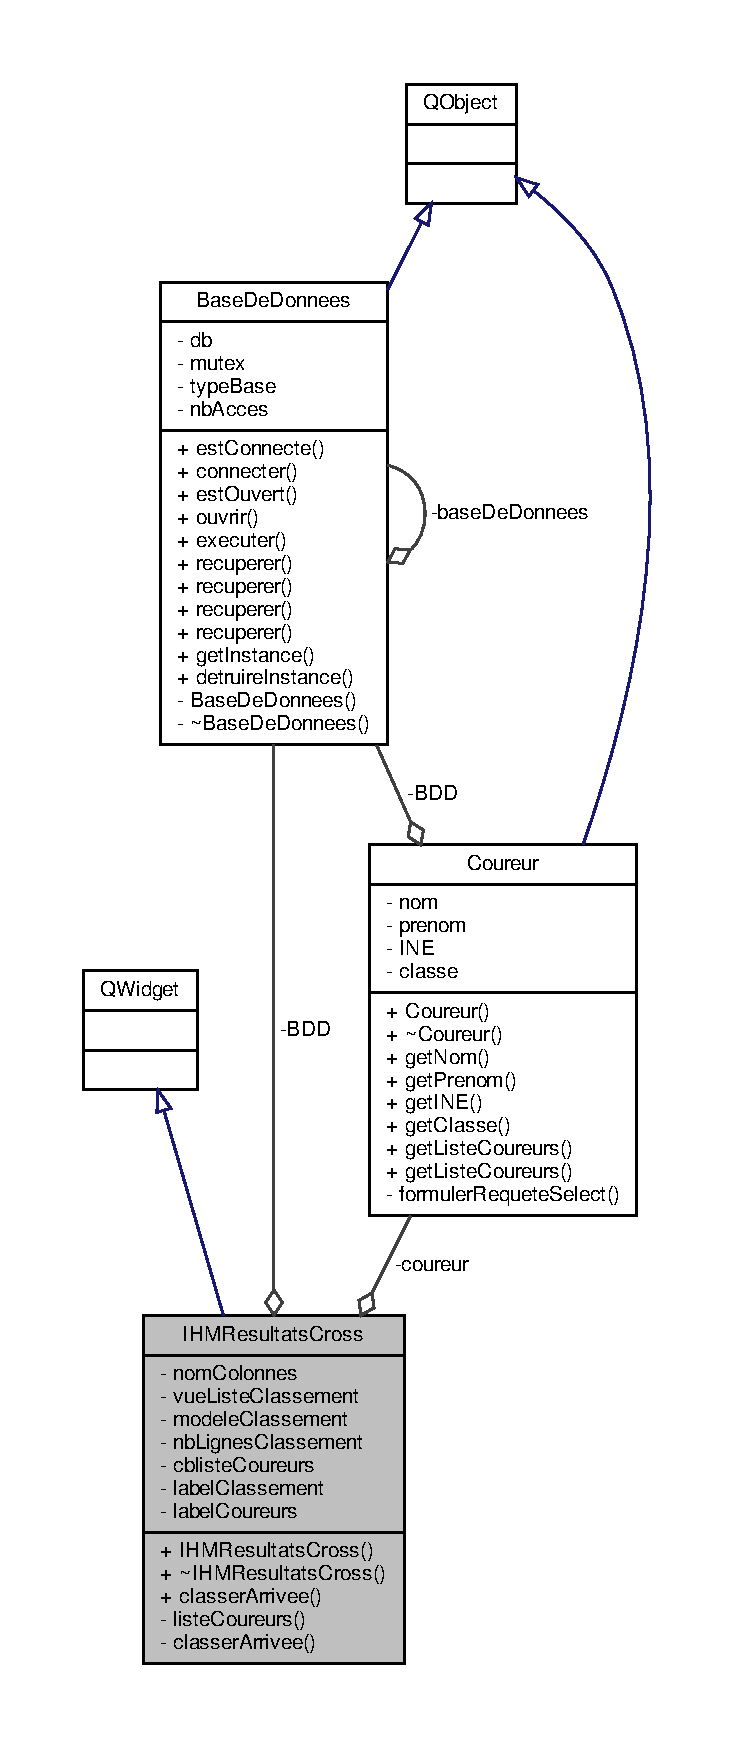
\includegraphics[height=550pt]{class_i_h_m_resultats_cross__coll__graph}
\end{center}
\end{figure}
\subsubsection*{Fonctions membres publiques}
\begin{DoxyCompactItemize}
\item 
\hyperlink{class_i_h_m_resultats_cross_a94afa0356ebc98e497dfecca3e1bb00b}{I\+H\+M\+Resultats\+Cross} (\hyperlink{class_q_widget}{Q\+Widget} $\ast$parent=nullptr)
\begin{DoxyCompactList}\small\item\em Constructeur de la fenêtre principale. \end{DoxyCompactList}\item 
\hyperlink{class_i_h_m_resultats_cross_a62afe926862fddcb340e4a2c57c3cddf}{$\sim$\+I\+H\+M\+Resultats\+Cross} ()
\begin{DoxyCompactList}\small\item\em Destructeur de la fenêtre principale. \end{DoxyCompactList}\item 
void \hyperlink{class_i_h_m_resultats_cross_a4311c35a2869a24be1a06d7410623eda}{classer\+Arrivee} ()
\end{DoxyCompactItemize}
\subsubsection*{Connecteurs privés}
\begin{DoxyCompactItemize}
\item 
void \hyperlink{class_i_h_m_resultats_cross_a5f4a74c4c024aaa9d39050ac176c9e37}{classer\+Arrivee} (Q\+String\+List classement\+Coureurs)
\end{DoxyCompactItemize}
\subsubsection*{Fonctions membres privées}
\begin{DoxyCompactItemize}
\item 
void \hyperlink{class_i_h_m_resultats_cross_a5e8e7f363a93e1e5e6b3c5eb0ad29c28}{liste\+Coureurs} ()
\end{DoxyCompactItemize}
\subsubsection*{Attributs privés}
\begin{DoxyCompactItemize}
\item 
Q\+String\+List \hyperlink{class_i_h_m_resultats_cross_abfda0d5dc4b65c0525a94a74faf68ce0}{nom\+Colonnes}
\item 
\hyperlink{class_base_de_donnees}{Base\+De\+Donnees} $\ast$ \hyperlink{class_i_h_m_resultats_cross_a3f27f95ca0fb27d1a46814d2fddfc3b1}{B\+DD}
\begin{DoxyCompactList}\small\item\em agrégation Base\+De\+Donnee \end{DoxyCompactList}\item 
Q\+Table\+View $\ast$ \hyperlink{class_i_h_m_resultats_cross_a8f35fc63f8c3a1351658d3148daf13e0}{vue\+Liste\+Classement}
\begin{DoxyCompactList}\small\item\em Tableau classement. \end{DoxyCompactList}\item 
Q\+Standard\+Item\+Model $\ast$ \hyperlink{class_i_h_m_resultats_cross_a9d4e02948f64b6d9fef422d7f5a2b9b5}{modele\+Classement}
\item 
int \hyperlink{class_i_h_m_resultats_cross_a696f826387c8fa8b9925ca468a52482e}{nb\+Lignes\+Classement}
\item 
\hyperlink{class_coureur}{Coureur} $\ast$ \hyperlink{class_i_h_m_resultats_cross_ab637383c58d9ce784aec696ccd69d709}{coureur}
\begin{DoxyCompactList}\small\item\em agrégation coureur \end{DoxyCompactList}\item 
Q\+Combo\+Box $\ast$ \hyperlink{class_i_h_m_resultats_cross_ae1190e783fc117504abf614fe170ad54}{cbliste\+Coureurs}
\begin{DoxyCompactList}\small\item\em Combobox contenant les différentes coureurs dans la base de données. \end{DoxyCompactList}\item 
Q\+Label $\ast$ \hyperlink{class_i_h_m_resultats_cross_a455bc28e3605cd327067be2db255c911}{label\+Classement}
\item 
Q\+Label $\ast$ \hyperlink{class_i_h_m_resultats_cross_a0cec9448e3ac680fd93cff9c4c709e1b}{label\+Coureurs}
\end{DoxyCompactItemize}


\subsubsection{Description détaillée}
La fenêtre principale de l\textquotesingle{}application Resultats-\/\+Cross. 

\begin{DoxyAuthor}{Auteur}
Suzie Turlin
\end{DoxyAuthor}
\begin{DoxyVersion}{Version}
0.\+1 
\end{DoxyVersion}


\subsubsection{Documentation des constructeurs et destructeur}
\mbox{\Hypertarget{class_i_h_m_resultats_cross_a94afa0356ebc98e497dfecca3e1bb00b}\label{class_i_h_m_resultats_cross_a94afa0356ebc98e497dfecca3e1bb00b}} 
\index{I\+H\+M\+Resultats\+Cross@{I\+H\+M\+Resultats\+Cross}!I\+H\+M\+Resultats\+Cross@{I\+H\+M\+Resultats\+Cross}}
\index{I\+H\+M\+Resultats\+Cross@{I\+H\+M\+Resultats\+Cross}!I\+H\+M\+Resultats\+Cross@{I\+H\+M\+Resultats\+Cross}}
\paragraph{\texorpdfstring{I\+H\+M\+Resultats\+Cross()}{IHMResultatsCross()}}
{\footnotesize\ttfamily I\+H\+M\+Resultats\+Cross\+::\+I\+H\+M\+Resultats\+Cross (\begin{DoxyParamCaption}\item[{\hyperlink{class_q_widget}{Q\+Widget} $\ast$}]{parent = {\ttfamily nullptr} }\end{DoxyParamCaption})}



Constructeur de la fenêtre principale. 


\begin{DoxyParams}{Paramètres}
{\em parent} & \hyperlink{class_q_object}{Q\+Object} Adresse de l\textquotesingle{}objet Qt parent (0 = pas de parent car c\textquotesingle{}est la fenêtre principale) \\
\hline
\end{DoxyParams}
\begin{DoxyRefDesc}{A faire}
\item[\hyperlink{todo__todo000002}{A faire}]Définir le contenu de l\textquotesingle{}I\+HM \end{DoxyRefDesc}


Références \hyperlink{class_i_h_m_resultats_cross_a3f27f95ca0fb27d1a46814d2fddfc3b1}{B\+DD}, \hyperlink{class_i_h_m_resultats_cross_ae1190e783fc117504abf614fe170ad54}{cbliste\+Coureurs}, \hyperlink{class_base_de_donnees_ab2e092285ccc0ee1cce61a1774218561}{Base\+De\+Donnees\+::connecter()}, \hyperlink{class_i_h_m_resultats_cross_ab637383c58d9ce784aec696ccd69d709}{coureur}, \hyperlink{class_base_de_donnees_a00388973f3ec42e5c8e76e7af7e124b2}{Base\+De\+Donnees\+::est\+Connecte()}, \hyperlink{class_base_de_donnees_a80028aa2b6b4fbf30fb2e36357b7d3d3}{Base\+De\+Donnees\+::get\+Instance()}, \hyperlink{class_i_h_m_resultats_cross_a455bc28e3605cd327067be2db255c911}{label\+Classement}, \hyperlink{class_i_h_m_resultats_cross_a0cec9448e3ac680fd93cff9c4c709e1b}{label\+Coureurs}, \hyperlink{class_i_h_m_resultats_cross_a9d4e02948f64b6d9fef422d7f5a2b9b5}{modele\+Classement}, \hyperlink{class_i_h_m_resultats_cross_abfda0d5dc4b65c0525a94a74faf68ce0}{nom\+Colonnes}, \hyperlink{ihmchronocross_8h_a407f067284fd7ac16426ac29cbfcd356}{T\+A\+I\+L\+L\+E\+T\+E\+X\+T\+E\+L\+A\+B\+EL}, et \hyperlink{class_i_h_m_resultats_cross_a8f35fc63f8c3a1351658d3148daf13e0}{vue\+Liste\+Classement}.


\begin{DoxyCode}
00025                                                     : \hyperlink{class_q_widget}{QWidget}(parent)
00026 \{
00031     \hyperlink{class_i_h_m_resultats_cross_ab637383c58d9ce784aec696ccd69d709}{coureur} = \textcolor{keyword}{new} \hyperlink{class_coureur}{Coureur}(\textcolor{keyword}{this});
00032 
00033     \hyperlink{class_i_h_m_resultats_cross_a3f27f95ca0fb27d1a46814d2fddfc3b1}{BDD} = \hyperlink{class_base_de_donnees_a80028aa2b6b4fbf30fb2e36357b7d3d3}{BaseDeDonnees::getInstance}();
00034     \textcolor{keywordflow}{if}(!\hyperlink{class_i_h_m_resultats_cross_a3f27f95ca0fb27d1a46814d2fddfc3b1}{BDD}->\hyperlink{class_base_de_donnees_a00388973f3ec42e5c8e76e7af7e124b2}{estConnecte}())
00035         \hyperlink{class_i_h_m_resultats_cross_a3f27f95ca0fb27d1a46814d2fddfc3b1}{BDD}->\hyperlink{class_base_de_donnees_ab2e092285ccc0ee1cce61a1774218561}{connecter}(\textcolor{stringliteral}{"Resultats-Cross"});
00036 
00037     \hyperlink{class_i_h_m_resultats_cross_a8f35fc63f8c3a1351658d3148daf13e0}{vueListeClassement} = \textcolor{keyword}{new} QTableView(\textcolor{keyword}{this});
00038     \hyperlink{class_i_h_m_resultats_cross_a9d4e02948f64b6d9fef422d7f5a2b9b5}{modeleClassement} = \textcolor{keyword}{new} QStandardItemModel(1, 4);
00039     \hyperlink{class_i_h_m_resultats_cross_abfda0d5dc4b65c0525a94a74faf68ce0}{nomColonnes} << \textcolor{stringliteral}{"Nom"} << \textcolor{stringliteral}{"Prénom"} << \textcolor{stringliteral}{"Classe"} << \textcolor{stringliteral}{"INE"};
00040     \hyperlink{class_i_h_m_resultats_cross_a9d4e02948f64b6d9fef422d7f5a2b9b5}{modeleClassement}->setHorizontalHeaderLabels(\hyperlink{class_i_h_m_resultats_cross_abfda0d5dc4b65c0525a94a74faf68ce0}{nomColonnes});
00041     \hyperlink{class_i_h_m_resultats_cross_a8f35fc63f8c3a1351658d3148daf13e0}{vueListeClassement}->setModel(\hyperlink{class_i_h_m_resultats_cross_a9d4e02948f64b6d9fef422d7f5a2b9b5}{modeleClassement});
00042     \hyperlink{class_i_h_m_resultats_cross_a8f35fc63f8c3a1351658d3148daf13e0}{vueListeClassement}->setEditTriggers(QAbstractItemView::NoEditTriggers);
00043     \hyperlink{class_i_h_m_resultats_cross_a8f35fc63f8c3a1351658d3148daf13e0}{vueListeClassement}->setFixedSize(this->width(), this->height());
00044 
00045     \hyperlink{class_i_h_m_resultats_cross_a8f35fc63f8c3a1351658d3148daf13e0}{vueListeClassement}->show();
00046 
00047     \textcolor{comment}{// les widgets}
00048 
00049     \textcolor{comment}{// défini la taille du text dans les QPushButtons}
00050     \textcolor{comment}{/*QFont texteBouton;}
00051 \textcolor{comment}{    texteBouton.setPointSize(TAILLETEXTEBUTON);}
00052 \textcolor{comment}{}
00053 \textcolor{comment}{    bAjouter = new QPushButton(QString::fromUtf8("Démarrer"), this);}
00054 \textcolor{comment}{    bAjouter->setDefault(false);}
00055 \textcolor{comment}{    bAjouter->setEnabled(false);}
00056 \textcolor{comment}{    bAjouter->setFont(texteBouton);*/}
00057 
00058    \textcolor{comment}{/* cblisteCoureurs = new QComboBox(this);}
00059 \textcolor{comment}{    cblisteCoureurs->setFixedSize(this->width()*0.66, this->height()*0.08);}
00060 \textcolor{comment}{    cblisteCoureurs->addItem(("< Séléctionner Coureur >"));*/}
00061 
00062 
00063     \textcolor{comment}{// défini la taille du text des labels}
00064     QFont texteLabel;
00065     texteLabel.setPointSize(\hyperlink{ihmchronocross_8h_a407f067284fd7ac16426ac29cbfcd356}{TAILLETEXTELABEL});
00066 
00067     \hyperlink{class_i_h_m_resultats_cross_a455bc28e3605cd327067be2db255c911}{labelClassement} = \textcolor{keyword}{new} QLabel(tr(\textcolor{stringliteral}{"Classement : "}), \textcolor{keyword}{this});
00068     \hyperlink{class_i_h_m_resultats_cross_a455bc28e3605cd327067be2db255c911}{labelClassement}->setFont(texteLabel);
00069     \hyperlink{class_i_h_m_resultats_cross_a0cec9448e3ac680fd93cff9c4c709e1b}{labelCoureurs} = \textcolor{keyword}{new} QLabel(tr(\textcolor{stringliteral}{"Coureurs : "}), \textcolor{keyword}{this});
00070     \hyperlink{class_i_h_m_resultats_cross_a0cec9448e3ac680fd93cff9c4c709e1b}{labelCoureurs}->setFont(texteLabel);
00071 
00072     QVBoxLayout *classementLayout = \textcolor{keyword}{new} QVBoxLayout;
00073     classementLayout->addWidget(\hyperlink{class_i_h_m_resultats_cross_a455bc28e3605cd327067be2db255c911}{labelClassement});
00074     classementLayout->addWidget(\hyperlink{class_i_h_m_resultats_cross_a8f35fc63f8c3a1351658d3148daf13e0}{vueListeClassement});
00075 
00076     \textcolor{comment}{// le positionnement des widgets}
00077     QHBoxLayout *listesLayout = \textcolor{keyword}{new} QHBoxLayout;
00078     \textcolor{comment}{//QHBoxLayout *boutonsLayout = new QHBoxLayout;}
00079 
00080     listesLayout->addWidget(\hyperlink{class_i_h_m_resultats_cross_ae1190e783fc117504abf614fe170ad54}{cblisteCoureurs});
00081     listesLayout->addWidget(\hyperlink{class_i_h_m_resultats_cross_a0cec9448e3ac680fd93cff9c4c709e1b}{labelCoureurs});
00082 
00083     QVBoxLayout *mainLayout = \textcolor{keyword}{new} QVBoxLayout;
00084     mainLayout->addLayout(listesLayout);
00085 
00086     setLayout(mainLayout);
00087     setWindowTitle(tr(\textcolor{stringliteral}{"Résultat-Cross"}));
00088     setContextMenuPolicy(Qt::ActionsContextMenu);
00089 
00090 
00091     \textcolor{comment}{//boutonsLayout->addWidget(bAjouter);}
00092     \textcolor{comment}{//boutonsLayout->setContentsMargins(0, 0, 0, 20); // G H D B}
00093 
00094     \textcolor{comment}{// Les labels}
00095 
00096     \textcolor{comment}{// Les connexions}
00097 
00098     \textcolor{comment}{// connect(bDemarrer, SIGNAL(clicked()), this, SLOT(coureur()));}
00099 
00100     showMaximized(); \textcolor{comment}{// Fenêtre d'ouverture maximale}
00101 \}
\end{DoxyCode}
\mbox{\Hypertarget{class_i_h_m_resultats_cross_a62afe926862fddcb340e4a2c57c3cddf}\label{class_i_h_m_resultats_cross_a62afe926862fddcb340e4a2c57c3cddf}} 
\index{I\+H\+M\+Resultats\+Cross@{I\+H\+M\+Resultats\+Cross}!````~I\+H\+M\+Resultats\+Cross@{$\sim$\+I\+H\+M\+Resultats\+Cross}}
\index{````~I\+H\+M\+Resultats\+Cross@{$\sim$\+I\+H\+M\+Resultats\+Cross}!I\+H\+M\+Resultats\+Cross@{I\+H\+M\+Resultats\+Cross}}
\paragraph{\texorpdfstring{$\sim$\+I\+H\+M\+Resultats\+Cross()}{~IHMResultatsCross()}}
{\footnotesize\ttfamily I\+H\+M\+Resultats\+Cross\+::$\sim$\+I\+H\+M\+Resultats\+Cross (\begin{DoxyParamCaption}{ }\end{DoxyParamCaption})}



Destructeur de la fenêtre principale. 



Références \hyperlink{class_base_de_donnees_a457401c0816b888c77ce915997545f4e}{Base\+De\+Donnees\+::detruire\+Instance()}.


\begin{DoxyCode}
00110 \{
00111     \hyperlink{class_base_de_donnees_a457401c0816b888c77ce915997545f4e}{BaseDeDonnees::detruireInstance}();
00112     qDebug() << Q\_FUNC\_INFO;
00113 \}
\end{DoxyCode}


\subsubsection{Documentation des fonctions membres}
\mbox{\Hypertarget{class_i_h_m_resultats_cross_a4311c35a2869a24be1a06d7410623eda}\label{class_i_h_m_resultats_cross_a4311c35a2869a24be1a06d7410623eda}} 
\index{I\+H\+M\+Resultats\+Cross@{I\+H\+M\+Resultats\+Cross}!classer\+Arrivee@{classer\+Arrivee}}
\index{classer\+Arrivee@{classer\+Arrivee}!I\+H\+M\+Resultats\+Cross@{I\+H\+M\+Resultats\+Cross}}
\paragraph{\texorpdfstring{classer\+Arrivee()}{classerArrivee()}\hspace{0.1cm}{\footnotesize\ttfamily [1/2]}}
{\footnotesize\ttfamily void I\+H\+M\+Resultats\+Cross\+::classer\+Arrivee (\begin{DoxyParamCaption}{ }\end{DoxyParamCaption})}

\mbox{\Hypertarget{class_i_h_m_resultats_cross_a5f4a74c4c024aaa9d39050ac176c9e37}\label{class_i_h_m_resultats_cross_a5f4a74c4c024aaa9d39050ac176c9e37}} 
\index{I\+H\+M\+Resultats\+Cross@{I\+H\+M\+Resultats\+Cross}!classer\+Arrivee@{classer\+Arrivee}}
\index{classer\+Arrivee@{classer\+Arrivee}!I\+H\+M\+Resultats\+Cross@{I\+H\+M\+Resultats\+Cross}}
\paragraph{\texorpdfstring{classer\+Arrivee}{classerArrivee}\hspace{0.1cm}{\footnotesize\ttfamily [2/2]}}
{\footnotesize\ttfamily void I\+H\+M\+Resultats\+Cross\+::classer\+Arrivee (\begin{DoxyParamCaption}\item[{Q\+String\+List}]{classement\+Coureurs }\end{DoxyParamCaption})\hspace{0.3cm}{\ttfamily [private]}, {\ttfamily [slot]}}



Références \hyperlink{ihmchronocross_8h_a114680edc01528f77bb689b0a2ca18a2}{C\+O\+L\+O\+N\+N\+E\+\_\+\+C\+L\+A\+S\+SE}, \hyperlink{ihmgestioncross_8h_aa8208c9f9fd2ea2418e4b7bb28175f80}{C\+O\+L\+O\+N\+N\+E\+\_\+\+I\+NE}, \hyperlink{ihmchronocross_8h_aeee76385895c145ef5a633e6c6812603}{C\+O\+L\+O\+N\+N\+E\+\_\+\+N\+OM}, \hyperlink{ihmchronocross_8h_a5d6f240d26209cd66db8aa5e1aac62f9}{C\+O\+L\+O\+N\+N\+E\+\_\+\+P\+R\+E\+N\+OM}, \hyperlink{ihmchronocross_8h_a104dfa4cfc656a690caaec36fd4d3e2d}{I\+N\+F\+O\+\_\+\+C\+O\+U\+R\+E\+U\+R\+\_\+\+C\+L\+A\+S\+SE}, \hyperlink{ihmgestioncross_8h_a2e5435ad2b0c61674b2dad6c0ea46301}{I\+N\+F\+O\+\_\+\+C\+O\+U\+R\+E\+U\+R\+\_\+\+I\+NE}, \hyperlink{ihmchronocross_8h_a71b99ea06ae916bcd158edbd441c8c24}{I\+N\+F\+O\+\_\+\+C\+O\+U\+R\+E\+U\+R\+\_\+\+N\+OM}, \hyperlink{ihmchronocross_8h_a68fd2611ad0ef66da1a71726675067e7}{I\+N\+F\+O\+\_\+\+C\+O\+U\+R\+E\+U\+R\+\_\+\+P\+R\+E\+N\+OM}, \hyperlink{class_i_h_m_resultats_cross_a9d4e02948f64b6d9fef422d7f5a2b9b5}{modele\+Classement}, \hyperlink{class_i_h_m_resultats_cross_a696f826387c8fa8b9925ca468a52482e}{nb\+Lignes\+Classement}, et \hyperlink{class_i_h_m_resultats_cross_a8f35fc63f8c3a1351658d3148daf13e0}{vue\+Liste\+Classement}.


\begin{DoxyCode}
00117 \{
00118     qDebug() << Q\_FUNC\_INFO << informationCoureur;
00119     \textcolor{comment}{//informationCoureur[Nom, Prenom, Classe, INE]}
00120     \textcolor{comment}{// Redimensionner automatiquement la colonne pour occuper l'espace disponible}
00121 
00122     \hyperlink{class_i_h_m_resultats_cross_a8f35fc63f8c3a1351658d3148daf13e0}{vueListeClassement}->horizontalHeader()->setSectionResizeMode(QHeaderView::Stretch);
00123     \hyperlink{class_i_h_m_resultats_cross_a696f826387c8fa8b9925ca468a52482e}{nbLignesClassement} = 1 - \hyperlink{class_i_h_m_resultats_cross_a9d4e02948f64b6d9fef422d7f5a2b9b5}{modeleClassement}->rowCount();
00124 
00125 
00126     QStandardItem *nom = \textcolor{keyword}{new} QStandardItem(informationCoureur.at(
      \hyperlink{ihmchronocross_8h_a71b99ea06ae916bcd158edbd441c8c24}{INFO\_COUREUR\_NOM}));
00127     QStandardItem *prenom = \textcolor{keyword}{new} QStandardItem(informationCoureur.at(
      \hyperlink{ihmchronocross_8h_a68fd2611ad0ef66da1a71726675067e7}{INFO\_COUREUR\_PRENOM}));
00128     QStandardItem *classe = \textcolor{keyword}{new} QStandardItem(informationCoureur.at(
      \hyperlink{ihmchronocross_8h_a104dfa4cfc656a690caaec36fd4d3e2d}{INFO\_COUREUR\_CLASSE}));
00129     QStandardItem *INE = \textcolor{keyword}{new} QStandardItem(informationCoureur.at(
      \hyperlink{ihmgestioncross_8h_a2e5435ad2b0c61674b2dad6c0ea46301}{INFO\_COUREUR\_INE}));
00130 
00131 
00132     \hyperlink{class_i_h_m_resultats_cross_a9d4e02948f64b6d9fef422d7f5a2b9b5}{modeleClassement}->setItem(\hyperlink{class_i_h_m_resultats_cross_a696f826387c8fa8b9925ca468a52482e}{nbLignesClassement}, 
      \hyperlink{ihmchronocross_8h_aeee76385895c145ef5a633e6c6812603}{COLONNE\_NOM}, nom);
00133     \hyperlink{class_i_h_m_resultats_cross_a9d4e02948f64b6d9fef422d7f5a2b9b5}{modeleClassement}->setItem(\hyperlink{class_i_h_m_resultats_cross_a696f826387c8fa8b9925ca468a52482e}{nbLignesClassement}, 
      \hyperlink{ihmchronocross_8h_a5d6f240d26209cd66db8aa5e1aac62f9}{COLONNE\_PRENOM}, prenom);
00134     \hyperlink{class_i_h_m_resultats_cross_a9d4e02948f64b6d9fef422d7f5a2b9b5}{modeleClassement}->setItem(\hyperlink{class_i_h_m_resultats_cross_a696f826387c8fa8b9925ca468a52482e}{nbLignesClassement}, 
      \hyperlink{ihmchronocross_8h_a114680edc01528f77bb689b0a2ca18a2}{COLONNE\_CLASSE}, classe);
00135     \hyperlink{class_i_h_m_resultats_cross_a9d4e02948f64b6d9fef422d7f5a2b9b5}{modeleClassement}->setItem(\hyperlink{class_i_h_m_resultats_cross_a696f826387c8fa8b9925ca468a52482e}{nbLignesClassement}, 
      \hyperlink{ihmgestioncross_8h_aa8208c9f9fd2ea2418e4b7bb28175f80}{COLONNE\_INE}, INE);
00136     \hyperlink{class_i_h_m_resultats_cross_a696f826387c8fa8b9925ca468a52482e}{nbLignesClassement} += 1;
00137 \}
\end{DoxyCode}
\mbox{\Hypertarget{class_i_h_m_resultats_cross_a5e8e7f363a93e1e5e6b3c5eb0ad29c28}\label{class_i_h_m_resultats_cross_a5e8e7f363a93e1e5e6b3c5eb0ad29c28}} 
\index{I\+H\+M\+Resultats\+Cross@{I\+H\+M\+Resultats\+Cross}!liste\+Coureurs@{liste\+Coureurs}}
\index{liste\+Coureurs@{liste\+Coureurs}!I\+H\+M\+Resultats\+Cross@{I\+H\+M\+Resultats\+Cross}}
\paragraph{\texorpdfstring{liste\+Coureurs()}{listeCoureurs()}}
{\footnotesize\ttfamily void I\+H\+M\+Resultats\+Cross\+::liste\+Coureurs (\begin{DoxyParamCaption}{ }\end{DoxyParamCaption})\hspace{0.3cm}{\ttfamily [private]}}



\subsubsection{Documentation des données membres}
\mbox{\Hypertarget{class_i_h_m_resultats_cross_a3f27f95ca0fb27d1a46814d2fddfc3b1}\label{class_i_h_m_resultats_cross_a3f27f95ca0fb27d1a46814d2fddfc3b1}} 
\index{I\+H\+M\+Resultats\+Cross@{I\+H\+M\+Resultats\+Cross}!B\+DD@{B\+DD}}
\index{B\+DD@{B\+DD}!I\+H\+M\+Resultats\+Cross@{I\+H\+M\+Resultats\+Cross}}
\paragraph{\texorpdfstring{B\+DD}{BDD}}
{\footnotesize\ttfamily \hyperlink{class_base_de_donnees}{Base\+De\+Donnees}$\ast$ I\+H\+M\+Resultats\+Cross\+::\+B\+DD\hspace{0.3cm}{\ttfamily [private]}}



agrégation Base\+De\+Donnee 



Référencé par \hyperlink{class_i_h_m_resultats_cross_a94afa0356ebc98e497dfecca3e1bb00b}{I\+H\+M\+Resultats\+Cross()}.

\mbox{\Hypertarget{class_i_h_m_resultats_cross_ae1190e783fc117504abf614fe170ad54}\label{class_i_h_m_resultats_cross_ae1190e783fc117504abf614fe170ad54}} 
\index{I\+H\+M\+Resultats\+Cross@{I\+H\+M\+Resultats\+Cross}!cbliste\+Coureurs@{cbliste\+Coureurs}}
\index{cbliste\+Coureurs@{cbliste\+Coureurs}!I\+H\+M\+Resultats\+Cross@{I\+H\+M\+Resultats\+Cross}}
\paragraph{\texorpdfstring{cbliste\+Coureurs}{cblisteCoureurs}}
{\footnotesize\ttfamily Q\+Combo\+Box$\ast$ I\+H\+M\+Resultats\+Cross\+::cbliste\+Coureurs\hspace{0.3cm}{\ttfamily [private]}}



Combobox contenant les différentes coureurs dans la base de données. 



Référencé par \hyperlink{class_i_h_m_resultats_cross_a94afa0356ebc98e497dfecca3e1bb00b}{I\+H\+M\+Resultats\+Cross()}.

\mbox{\Hypertarget{class_i_h_m_resultats_cross_ab637383c58d9ce784aec696ccd69d709}\label{class_i_h_m_resultats_cross_ab637383c58d9ce784aec696ccd69d709}} 
\index{I\+H\+M\+Resultats\+Cross@{I\+H\+M\+Resultats\+Cross}!coureur@{coureur}}
\index{coureur@{coureur}!I\+H\+M\+Resultats\+Cross@{I\+H\+M\+Resultats\+Cross}}
\paragraph{\texorpdfstring{coureur}{coureur}}
{\footnotesize\ttfamily \hyperlink{class_coureur}{Coureur}$\ast$ I\+H\+M\+Resultats\+Cross\+::coureur\hspace{0.3cm}{\ttfamily [private]}}



agrégation coureur 



Référencé par \hyperlink{class_i_h_m_resultats_cross_a94afa0356ebc98e497dfecca3e1bb00b}{I\+H\+M\+Resultats\+Cross()}.

\mbox{\Hypertarget{class_i_h_m_resultats_cross_a455bc28e3605cd327067be2db255c911}\label{class_i_h_m_resultats_cross_a455bc28e3605cd327067be2db255c911}} 
\index{I\+H\+M\+Resultats\+Cross@{I\+H\+M\+Resultats\+Cross}!label\+Classement@{label\+Classement}}
\index{label\+Classement@{label\+Classement}!I\+H\+M\+Resultats\+Cross@{I\+H\+M\+Resultats\+Cross}}
\paragraph{\texorpdfstring{label\+Classement}{labelClassement}}
{\footnotesize\ttfamily Q\+Label$\ast$ I\+H\+M\+Resultats\+Cross\+::label\+Classement\hspace{0.3cm}{\ttfamily [private]}}



Référencé par \hyperlink{class_i_h_m_resultats_cross_a94afa0356ebc98e497dfecca3e1bb00b}{I\+H\+M\+Resultats\+Cross()}.

\mbox{\Hypertarget{class_i_h_m_resultats_cross_a0cec9448e3ac680fd93cff9c4c709e1b}\label{class_i_h_m_resultats_cross_a0cec9448e3ac680fd93cff9c4c709e1b}} 
\index{I\+H\+M\+Resultats\+Cross@{I\+H\+M\+Resultats\+Cross}!label\+Coureurs@{label\+Coureurs}}
\index{label\+Coureurs@{label\+Coureurs}!I\+H\+M\+Resultats\+Cross@{I\+H\+M\+Resultats\+Cross}}
\paragraph{\texorpdfstring{label\+Coureurs}{labelCoureurs}}
{\footnotesize\ttfamily Q\+Label$\ast$ I\+H\+M\+Resultats\+Cross\+::label\+Coureurs\hspace{0.3cm}{\ttfamily [private]}}



Référencé par \hyperlink{class_i_h_m_resultats_cross_a94afa0356ebc98e497dfecca3e1bb00b}{I\+H\+M\+Resultats\+Cross()}.

\mbox{\Hypertarget{class_i_h_m_resultats_cross_a9d4e02948f64b6d9fef422d7f5a2b9b5}\label{class_i_h_m_resultats_cross_a9d4e02948f64b6d9fef422d7f5a2b9b5}} 
\index{I\+H\+M\+Resultats\+Cross@{I\+H\+M\+Resultats\+Cross}!modele\+Classement@{modele\+Classement}}
\index{modele\+Classement@{modele\+Classement}!I\+H\+M\+Resultats\+Cross@{I\+H\+M\+Resultats\+Cross}}
\paragraph{\texorpdfstring{modele\+Classement}{modeleClassement}}
{\footnotesize\ttfamily Q\+Standard\+Item\+Model$\ast$ I\+H\+M\+Resultats\+Cross\+::modele\+Classement\hspace{0.3cm}{\ttfamily [private]}}



Référencé par \hyperlink{class_i_h_m_resultats_cross_a5f4a74c4c024aaa9d39050ac176c9e37}{classer\+Arrivee()}, et \hyperlink{class_i_h_m_resultats_cross_a94afa0356ebc98e497dfecca3e1bb00b}{I\+H\+M\+Resultats\+Cross()}.

\mbox{\Hypertarget{class_i_h_m_resultats_cross_a696f826387c8fa8b9925ca468a52482e}\label{class_i_h_m_resultats_cross_a696f826387c8fa8b9925ca468a52482e}} 
\index{I\+H\+M\+Resultats\+Cross@{I\+H\+M\+Resultats\+Cross}!nb\+Lignes\+Classement@{nb\+Lignes\+Classement}}
\index{nb\+Lignes\+Classement@{nb\+Lignes\+Classement}!I\+H\+M\+Resultats\+Cross@{I\+H\+M\+Resultats\+Cross}}
\paragraph{\texorpdfstring{nb\+Lignes\+Classement}{nbLignesClassement}}
{\footnotesize\ttfamily int I\+H\+M\+Resultats\+Cross\+::nb\+Lignes\+Classement\hspace{0.3cm}{\ttfamily [private]}}



Référencé par \hyperlink{class_i_h_m_resultats_cross_a5f4a74c4c024aaa9d39050ac176c9e37}{classer\+Arrivee()}.

\mbox{\Hypertarget{class_i_h_m_resultats_cross_abfda0d5dc4b65c0525a94a74faf68ce0}\label{class_i_h_m_resultats_cross_abfda0d5dc4b65c0525a94a74faf68ce0}} 
\index{I\+H\+M\+Resultats\+Cross@{I\+H\+M\+Resultats\+Cross}!nom\+Colonnes@{nom\+Colonnes}}
\index{nom\+Colonnes@{nom\+Colonnes}!I\+H\+M\+Resultats\+Cross@{I\+H\+M\+Resultats\+Cross}}
\paragraph{\texorpdfstring{nom\+Colonnes}{nomColonnes}}
{\footnotesize\ttfamily Q\+String\+List I\+H\+M\+Resultats\+Cross\+::nom\+Colonnes\hspace{0.3cm}{\ttfamily [private]}}



Référencé par \hyperlink{class_i_h_m_resultats_cross_a94afa0356ebc98e497dfecca3e1bb00b}{I\+H\+M\+Resultats\+Cross()}.

\mbox{\Hypertarget{class_i_h_m_resultats_cross_a8f35fc63f8c3a1351658d3148daf13e0}\label{class_i_h_m_resultats_cross_a8f35fc63f8c3a1351658d3148daf13e0}} 
\index{I\+H\+M\+Resultats\+Cross@{I\+H\+M\+Resultats\+Cross}!vue\+Liste\+Classement@{vue\+Liste\+Classement}}
\index{vue\+Liste\+Classement@{vue\+Liste\+Classement}!I\+H\+M\+Resultats\+Cross@{I\+H\+M\+Resultats\+Cross}}
\paragraph{\texorpdfstring{vue\+Liste\+Classement}{vueListeClassement}}
{\footnotesize\ttfamily Q\+Table\+View$\ast$ I\+H\+M\+Resultats\+Cross\+::vue\+Liste\+Classement\hspace{0.3cm}{\ttfamily [private]}}



Tableau classement. 



Référencé par \hyperlink{class_i_h_m_resultats_cross_a5f4a74c4c024aaa9d39050ac176c9e37}{classer\+Arrivee()}, et \hyperlink{class_i_h_m_resultats_cross_a94afa0356ebc98e497dfecca3e1bb00b}{I\+H\+M\+Resultats\+Cross()}.



La documentation de cette classe a été générée à partir des fichiers suivants \+:\begin{DoxyCompactItemize}
\item 
\hyperlink{ihmresultatscross_8h}{ihmresultatscross.\+h}\item 
\hyperlink{ihmresultatscross_8cpp}{ihmresultatscross.\+cpp}\end{DoxyCompactItemize}

\hypertarget{class_q_object}{}\subsection{Référence de la classe Q\+Object}
\label{class_q_object}\index{Q\+Object@{Q\+Object}}


Graphe de collaboration de Q\+Object\+:\nopagebreak
\begin{figure}[H]
\begin{center}
\leavevmode
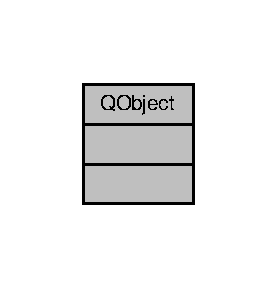
\includegraphics[width=133pt]{class_q_object__coll__graph}
\end{center}
\end{figure}


La documentation de cette classe a été générée à partir du fichier suivant \+:\begin{DoxyCompactItemize}
\item 
\hyperlink{coureur_8h}{coureur.\+h}\end{DoxyCompactItemize}

\hypertarget{class_q_widget}{}\subsection{Référence de la classe Q\+Widget}
\label{class_q_widget}\index{Q\+Widget@{Q\+Widget}}


Graphe de collaboration de Q\+Widget\+:\nopagebreak
\begin{figure}[H]
\begin{center}
\leavevmode
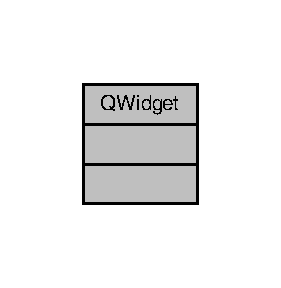
\includegraphics[width=135pt]{class_q_widget__coll__graph}
\end{center}
\end{figure}


La documentation de cette classe a été générée à partir du fichier suivant \+:\begin{DoxyCompactItemize}
\item 
\hyperlink{ihmchronocross_8h}{ihmchronocross.\+h}\end{DoxyCompactItemize}

\hypertarget{class_resultat}{}\subsection{Référence de la classe Resultat}
\label{class_resultat}\index{Resultat@{Resultat}}


{\ttfamily \#include $<$resultat.\+h$>$}



Graphe de collaboration de Resultat\+:\nopagebreak
\begin{figure}[H]
\begin{center}
\leavevmode
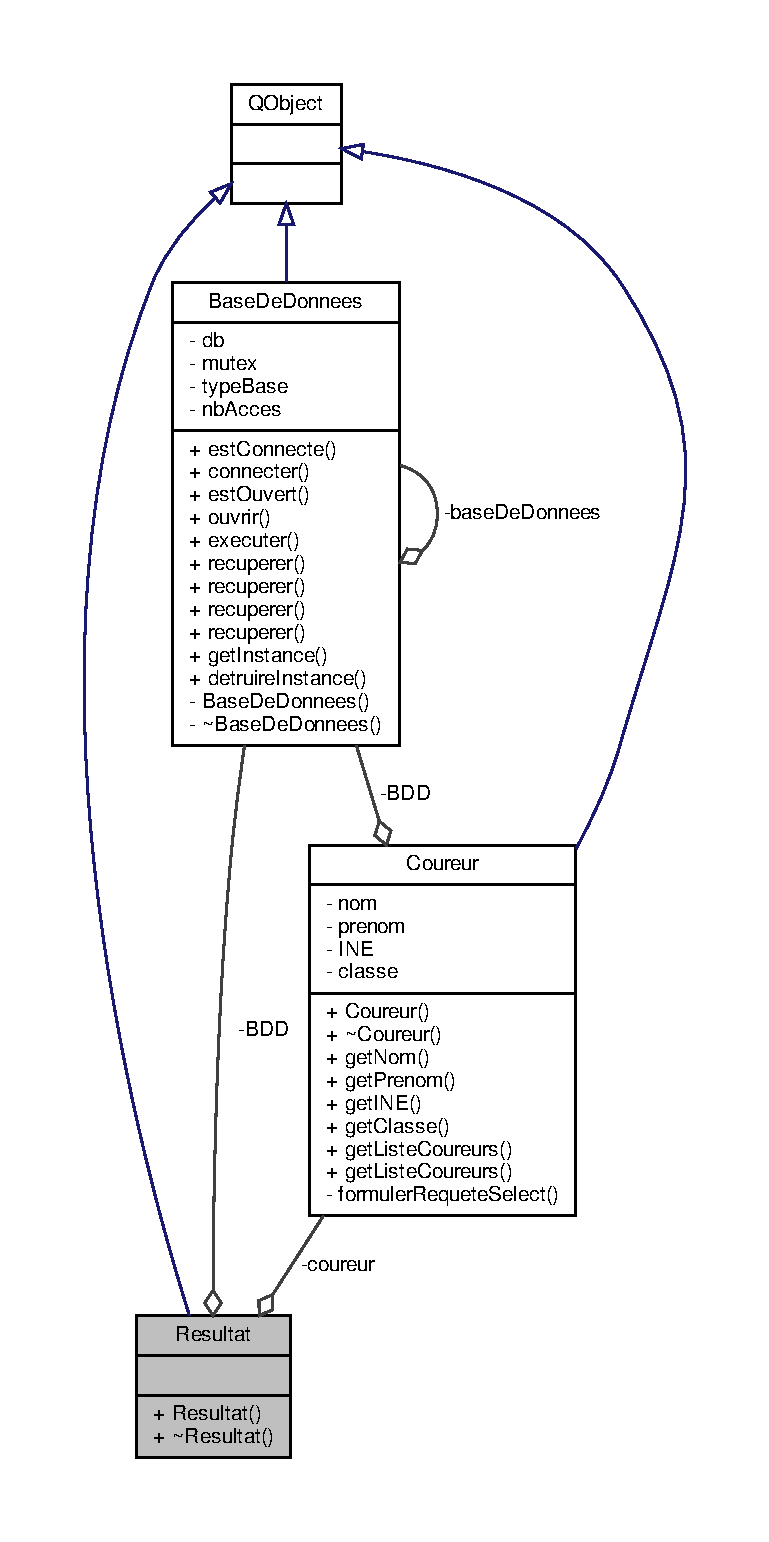
\includegraphics[height=550pt]{class_resultat__coll__graph}
\end{center}
\end{figure}
\subsubsection*{Fonctions membres publiques}
\begin{DoxyCompactItemize}
\item 
\hyperlink{class_resultat_a57e458f7abfc7463786ae9212bf55cd5}{Resultat} (\hyperlink{class_q_object}{Q\+Object} $\ast$parent=nullptr)
\begin{DoxyCompactList}\small\item\em \hyperlink{class_resultat}{Resultat}. \end{DoxyCompactList}\item 
\hyperlink{class_resultat_ae159333a3c5b89b8f307086bac618d7c}{$\sim$\+Resultat} ()
\end{DoxyCompactItemize}
\subsubsection*{Attributs privés}
\begin{DoxyCompactItemize}
\item 
\hyperlink{class_base_de_donnees}{Base\+De\+Donnees} $\ast$ \hyperlink{class_resultat_a25f2253e282cbedcd012c8496e219d86}{B\+DD}
\begin{DoxyCompactList}\small\item\em agrégation \hyperlink{class_base_de_donnees}{Base\+De\+Donnees} \end{DoxyCompactList}\item 
\hyperlink{class_coureur}{Coureur} $\ast$ \hyperlink{class_resultat_a89183a87b7855a9b7e3b628e2f689982}{coureur}
\begin{DoxyCompactList}\small\item\em association \hyperlink{class_coureur}{Coureur} \end{DoxyCompactList}\end{DoxyCompactItemize}


\subsubsection{Documentation des constructeurs et destructeur}
\mbox{\Hypertarget{class_resultat_a57e458f7abfc7463786ae9212bf55cd5}\label{class_resultat_a57e458f7abfc7463786ae9212bf55cd5}} 
\index{Resultat@{Resultat}!Resultat@{Resultat}}
\index{Resultat@{Resultat}!Resultat@{Resultat}}
\paragraph{\texorpdfstring{Resultat()}{Resultat()}}
{\footnotesize\ttfamily Resultat\+::\+Resultat (\begin{DoxyParamCaption}\item[{\hyperlink{class_q_object}{Q\+Object} $\ast$}]{parent = {\ttfamily nullptr} }\end{DoxyParamCaption})\hspace{0.3cm}{\ttfamily [explicit]}}



\hyperlink{class_resultat}{Resultat}. 


\begin{DoxyParams}{Paramètres}
{\em parent} & \hyperlink{class_q_object}{Q\+Object} Adresse de l\textquotesingle{}objet Qt parent \\
\hline
\end{DoxyParams}


Références \hyperlink{class_resultat_a25f2253e282cbedcd012c8496e219d86}{B\+DD}, \hyperlink{class_base_de_donnees_ab2e092285ccc0ee1cce61a1774218561}{Base\+De\+Donnees\+::connecter()}, \hyperlink{class_base_de_donnees_a00388973f3ec42e5c8e76e7af7e124b2}{Base\+De\+Donnees\+::est\+Connecte()}, et \hyperlink{class_base_de_donnees_a80028aa2b6b4fbf30fb2e36357b7d3d3}{Base\+De\+Donnees\+::get\+Instance()}.


\begin{DoxyCode}
00022                                   : \hyperlink{class_q_object}{QObject}(parent)
00023 \{
00024     \hyperlink{class_resultat_a25f2253e282cbedcd012c8496e219d86}{BDD} = \hyperlink{class_base_de_donnees_a80028aa2b6b4fbf30fb2e36357b7d3d3}{BaseDeDonnees::getInstance}();
00025     \textcolor{keywordflow}{if}(!\hyperlink{class_resultat_a25f2253e282cbedcd012c8496e219d86}{BDD}->\hyperlink{class_base_de_donnees_a00388973f3ec42e5c8e76e7af7e124b2}{estConnecte}())
00026         \hyperlink{class_resultat_a25f2253e282cbedcd012c8496e219d86}{BDD}->\hyperlink{class_base_de_donnees_ab2e092285ccc0ee1cce61a1774218561}{connecter}(\textcolor{stringliteral}{"Resultats-Cross"});
00027     qDebug() << Q\_FUNC\_INFO << \textcolor{stringliteral}{"Etat connection BDD : "} << \hyperlink{class_resultat_a25f2253e282cbedcd012c8496e219d86}{BDD}->\hyperlink{class_base_de_donnees_a00388973f3ec42e5c8e76e7af7e124b2}{estConnecte}();
00028 \}
\end{DoxyCode}
\mbox{\Hypertarget{class_resultat_ae159333a3c5b89b8f307086bac618d7c}\label{class_resultat_ae159333a3c5b89b8f307086bac618d7c}} 
\index{Resultat@{Resultat}!````~Resultat@{$\sim$\+Resultat}}
\index{````~Resultat@{$\sim$\+Resultat}!Resultat@{Resultat}}
\paragraph{\texorpdfstring{$\sim$\+Resultat()}{~Resultat()}}
{\footnotesize\ttfamily Resultat\+::$\sim$\+Resultat (\begin{DoxyParamCaption}{ }\end{DoxyParamCaption})}



Références \hyperlink{class_base_de_donnees_a457401c0816b888c77ce915997545f4e}{Base\+De\+Donnees\+::detruire\+Instance()}.


\begin{DoxyCode}
00031 \{
00032     \hyperlink{class_base_de_donnees_a457401c0816b888c77ce915997545f4e}{BaseDeDonnees::detruireInstance}();
00033     qDebug() << Q\_FUNC\_INFO;
00034 \}
\end{DoxyCode}


\subsubsection{Documentation des données membres}
\mbox{\Hypertarget{class_resultat_a25f2253e282cbedcd012c8496e219d86}\label{class_resultat_a25f2253e282cbedcd012c8496e219d86}} 
\index{Resultat@{Resultat}!B\+DD@{B\+DD}}
\index{B\+DD@{B\+DD}!Resultat@{Resultat}}
\paragraph{\texorpdfstring{B\+DD}{BDD}}
{\footnotesize\ttfamily \hyperlink{class_base_de_donnees}{Base\+De\+Donnees}$\ast$ Resultat\+::\+B\+DD\hspace{0.3cm}{\ttfamily [private]}}



agrégation \hyperlink{class_base_de_donnees}{Base\+De\+Donnees} 



Référencé par \hyperlink{class_resultat_a57e458f7abfc7463786ae9212bf55cd5}{Resultat()}.

\mbox{\Hypertarget{class_resultat_a89183a87b7855a9b7e3b628e2f689982}\label{class_resultat_a89183a87b7855a9b7e3b628e2f689982}} 
\index{Resultat@{Resultat}!coureur@{coureur}}
\index{coureur@{coureur}!Resultat@{Resultat}}
\paragraph{\texorpdfstring{coureur}{coureur}}
{\footnotesize\ttfamily \hyperlink{class_coureur}{Coureur}$\ast$ Resultat\+::coureur\hspace{0.3cm}{\ttfamily [private]}}



association \hyperlink{class_coureur}{Coureur} 



La documentation de cette classe a été générée à partir des fichiers suivants \+:\begin{DoxyCompactItemize}
\item 
\hyperlink{resultat_8h}{resultat.\+h}\item 
\hyperlink{resultat_8cpp}{resultat.\+cpp}\end{DoxyCompactItemize}

\section{Documentation des fichiers}
\hypertarget{basededonnees_8cpp}{}\subsection{Référence du fichier basededonnees.\+cpp}
\label{basededonnees_8cpp}\index{basededonnees.\+cpp@{basededonnees.\+cpp}}


Définition de la classe \hyperlink{class_base_de_donnees}{Base\+De\+Donnees}.  


{\ttfamily \#include \char`\"{}basededonnees.\+h\char`\"{}}\newline
{\ttfamily \#include $<$Q\+Debug$>$}\newline
{\ttfamily \#include $<$Q\+Message\+Box$>$}\newline


\subsubsection{Description détaillée}
Définition de la classe \hyperlink{class_base_de_donnees}{Base\+De\+Donnees}. 

\begin{DoxyAuthor}{Auteur}
Thierry Vaira
\end{DoxyAuthor}
\begin{DoxyVersion}{Version}
1.\+1 
\end{DoxyVersion}

\hypertarget{basededonnees_8h}{}\subsection{Référence du fichier basededonnees.\+h}
\label{basededonnees_8h}\index{basededonnees.\+h@{basededonnees.\+h}}


Déclaration de la classe \hyperlink{class_base_de_donnees}{Base\+De\+Donnees}.  


{\ttfamily \#include $<$Q\+Object$>$}\newline
{\ttfamily \#include $<$Qt\+Sql/\+Qt\+Sql$>$}\newline
{\ttfamily \#include $<$Q\+Sql\+Database$>$}\newline
{\ttfamily \#include $<$Q\+Mutex$>$}\newline
{\ttfamily \#include $<$Q\+String$>$}\newline
\subsubsection*{Classes}
\begin{DoxyCompactItemize}
\item 
class \hyperlink{class_base_de_donnees}{Base\+De\+Donnees}
\end{DoxyCompactItemize}
\subsubsection*{Macros}
\begin{DoxyCompactItemize}
\item 
\#define \hyperlink{basededonnees_8h_af06096ec4ec654090fa78ab359d4a0dd}{B\+D\+D\+\_\+\+H\+O\+S\+T\+N\+A\+ME}~\char`\"{}192.\+168.\+52.\+149\char`\"{}
\item 
\#define \hyperlink{basededonnees_8h_a88b5f5b81fa534553c68802384beff2c}{B\+D\+D\+\_\+\+U\+S\+E\+R\+N\+A\+ME}~\char`\"{}organisateur\char`\"{}
\item 
\#define \hyperlink{basededonnees_8h_ae2ded9166ed2553182545e97514c04f7}{B\+D\+D\+\_\+\+P\+A\+S\+S\+W\+O\+RD}~\char`\"{}password\char`\"{}
\end{DoxyCompactItemize}


\subsubsection{Description détaillée}
Déclaration de la classe \hyperlink{class_base_de_donnees}{Base\+De\+Donnees}. 

\begin{DoxyAuthor}{Auteur}
Thierry V\+A\+I\+RA
\end{DoxyAuthor}
\begin{DoxyVersion}{Version}
1.\+1 
\end{DoxyVersion}


\subsubsection{Documentation des macros}
\mbox{\Hypertarget{basededonnees_8h_af06096ec4ec654090fa78ab359d4a0dd}\label{basededonnees_8h_af06096ec4ec654090fa78ab359d4a0dd}} 
\index{basededonnees.\+h@{basededonnees.\+h}!B\+D\+D\+\_\+\+H\+O\+S\+T\+N\+A\+ME@{B\+D\+D\+\_\+\+H\+O\+S\+T\+N\+A\+ME}}
\index{B\+D\+D\+\_\+\+H\+O\+S\+T\+N\+A\+ME@{B\+D\+D\+\_\+\+H\+O\+S\+T\+N\+A\+ME}!basededonnees.\+h@{basededonnees.\+h}}
\paragraph{\texorpdfstring{B\+D\+D\+\_\+\+H\+O\+S\+T\+N\+A\+ME}{BDD\_HOSTNAME}}
{\footnotesize\ttfamily \#define B\+D\+D\+\_\+\+H\+O\+S\+T\+N\+A\+ME~\char`\"{}192.\+168.\+52.\+149\char`\"{}}

\mbox{\Hypertarget{basededonnees_8h_ae2ded9166ed2553182545e97514c04f7}\label{basededonnees_8h_ae2ded9166ed2553182545e97514c04f7}} 
\index{basededonnees.\+h@{basededonnees.\+h}!B\+D\+D\+\_\+\+P\+A\+S\+S\+W\+O\+RD@{B\+D\+D\+\_\+\+P\+A\+S\+S\+W\+O\+RD}}
\index{B\+D\+D\+\_\+\+P\+A\+S\+S\+W\+O\+RD@{B\+D\+D\+\_\+\+P\+A\+S\+S\+W\+O\+RD}!basededonnees.\+h@{basededonnees.\+h}}
\paragraph{\texorpdfstring{B\+D\+D\+\_\+\+P\+A\+S\+S\+W\+O\+RD}{BDD\_PASSWORD}}
{\footnotesize\ttfamily \#define B\+D\+D\+\_\+\+P\+A\+S\+S\+W\+O\+RD~\char`\"{}password\char`\"{}}

\mbox{\Hypertarget{basededonnees_8h_a88b5f5b81fa534553c68802384beff2c}\label{basededonnees_8h_a88b5f5b81fa534553c68802384beff2c}} 
\index{basededonnees.\+h@{basededonnees.\+h}!B\+D\+D\+\_\+\+U\+S\+E\+R\+N\+A\+ME@{B\+D\+D\+\_\+\+U\+S\+E\+R\+N\+A\+ME}}
\index{B\+D\+D\+\_\+\+U\+S\+E\+R\+N\+A\+ME@{B\+D\+D\+\_\+\+U\+S\+E\+R\+N\+A\+ME}!basededonnees.\+h@{basededonnees.\+h}}
\paragraph{\texorpdfstring{B\+D\+D\+\_\+\+U\+S\+E\+R\+N\+A\+ME}{BDD\_USERNAME}}
{\footnotesize\ttfamily \#define B\+D\+D\+\_\+\+U\+S\+E\+R\+N\+A\+ME~\char`\"{}organisateur\char`\"{}}


\hypertarget{_changelog_8md}{}\subsection{Référence du fichier Changelog.\+md}
\label{_changelog_8md}\index{Changelog.\+md@{Changelog.\+md}}

\hypertarget{chrono_8cpp}{}\subsection{Référence du fichier chrono.\+cpp}
\label{chrono_8cpp}\index{chrono.\+cpp@{chrono.\+cpp}}


Définition de la classe \hyperlink{class_chrono}{Chrono}.  


{\ttfamily \#include \char`\"{}chrono.\+h\char`\"{}}\newline
{\ttfamily \#include \char`\"{}unistd.\+h\char`\"{}}\newline


\subsubsection{Description détaillée}
Définition de la classe \hyperlink{class_chrono}{Chrono}. 

\begin{DoxyAuthor}{Auteur}
Michael Andreo
\end{DoxyAuthor}
\begin{DoxyVersion}{Version}
1.\+1 
\end{DoxyVersion}

\hypertarget{chrono_8h}{}\subsection{Référence du fichier chrono.\+h}
\label{chrono_8h}\index{chrono.\+h@{chrono.\+h}}


Déclaration de la classe \hyperlink{class_chrono}{Chrono}.  


{\ttfamily \#include $<$Q\+Object$>$}\newline
{\ttfamily \#include $<$Q\+Debug$>$}\newline
{\ttfamily \#include $<$Qt\+Serial\+Port/\+Q\+Serial\+Port$>$}\newline
\subsubsection*{Classes}
\begin{DoxyCompactItemize}
\item 
class \hyperlink{class_chrono}{Chrono}
\begin{DoxyCompactList}\small\item\em Déclaration de la classe \hyperlink{class_chrono}{Chrono}. \end{DoxyCompactList}\end{DoxyCompactItemize}
\subsubsection*{Macros}
\begin{DoxyCompactItemize}
\item 
\#define \hyperlink{chrono_8h_a614217d263be1fb1a5f76e2ff7be19a2}{P\+O\+RT}~\char`\"{}/dev/hl975\char`\"{}
\item 
\#define \hyperlink{chrono_8h_a51714542fe5fc5c442f126a96c568050}{M\+O\+D\+E\+C\+L\+O\+CK}~\char`\"{}\#WP 120 5\textbackslash{}t01\+A\+F\textbackslash{}r\textbackslash{}n\char`\"{}
\item 
\#define \hyperlink{chrono_8h_a6fd2c46c463ee5bf46edf6f117c277ec}{N\+E\+W\+S\+Y\+N\+C\+H\+RO}~\char`\"{}\#WC 007 02 00\+:00 01/01/01\textbackslash{}t048\+E\textbackslash{}r\textbackslash{}n\char`\"{}
\item 
\#define \hyperlink{chrono_8h_a4dcfb7100df159ff3082add0247cd3ee}{N\+E\+W\+R\+UN}~\char`\"{}\#WC 002\textbackslash{}t014\+C\textbackslash{}r\textbackslash{}n\char`\"{}
\item 
\#define \hyperlink{chrono_8h_a0130f9324a15a83d5609c874891d9d1f}{S\+T\+A\+R\+T\+M\+A\+N\+U\+A\+L\+S\+Y\+N\+C\+H\+RO}~\char`\"{}\#WC 008 01\textbackslash{}t01\+D3\textbackslash{}r\textbackslash{}n\char`\"{}
\item 
\#define \hyperlink{chrono_8h_aadc6271993e3725db8c6640289f8d2bb}{C\+L\+O\+S\+E\+R\+UN}~\char`\"{}\#WC 001\textbackslash{}t014\+B\textbackslash{}r\textbackslash{}n\char`\"{}
\item 
\#define \hyperlink{chrono_8h_a95708e00882b95a7b2d68b2f75c3913c}{M\+O\+D\+E\+ND}~\char`\"{}\#WP 120 3\textbackslash{}t01\+A\+D\textbackslash{}r\textbackslash{}n\char`\"{}
\item 
\#define \hyperlink{chrono_8h_a2c9f7b58ba826bd8365c9a611389fe42}{T\+R\+A\+M\+E\+\_\+\+A\+C\+Q\+U\+I\+T\+T\+E\+M\+E\+NT}~\char`\"{}AK\char`\"{}
\item 
\#define \hyperlink{chrono_8h_a1683bd797329c6abe147d1f3d5f2e67b}{T\+R\+A\+M\+E\+\_\+\+S\+Y\+N\+C\+H\+RO}~\char`\"{}TS\char`\"{}
\item 
\#define \hyperlink{chrono_8h_a58fe71fea35f1664c80e9a7b8f3a2b56}{T\+R\+A\+M\+E\+\_\+\+P\+A\+R\+A\+M\+E\+T\+R\+ES}~\char`\"{}\&P\char`\"{}
\item 
\#define \hyperlink{chrono_8h_af6d8d017aa1c07e0c9900e13a60959ba}{T\+R\+A\+M\+E\+\_\+\+T\+E\+M\+PS}~\char`\"{}TN\char`\"{}
\item 
\#define \hyperlink{chrono_8h_a24bef153968288b19cfda35989658fe1}{T\+R\+A\+M\+E\+\_\+\+C\+O\+U\+R\+S\+E\+\_\+\+T\+E\+R\+M\+I\+N\+EE}~\char`\"{}CL\char`\"{}
\item 
\#define \hyperlink{chrono_8h_af1a61de8ee28781dbc28e0d7d43c158e}{E\+T\+A\+T\+\_\+\+N\+O\+N\+S\+Y\+N\+C\+H\+RO}~0
\item 
\#define \hyperlink{chrono_8h_ac7f40e9c99ad9f32b52bbe642c29fa35}{E\+T\+A\+T\+\_\+\+M\+O\+D\+E\+C\+L\+O\+CK}~1
\item 
\#define \hyperlink{chrono_8h_ab4e7883be172f7dac0123a67e9c6c655}{E\+T\+A\+T\+\_\+\+N\+E\+W\+S\+Y\+N\+C\+H\+RO}~2
\item 
\#define \hyperlink{chrono_8h_a3870f0e4dd2af74ba5c110e419d65d99}{E\+T\+A\+T\+\_\+\+N\+E\+W\+R\+UN}~3
\item 
\#define \hyperlink{chrono_8h_ab6827e7b3f5ba7079e57df316b490544}{E\+T\+A\+T\+\_\+\+S\+T\+A\+R\+T\+M\+A\+N\+U\+A\+L\+S\+Y\+N\+C\+H\+RO}~4
\item 
\#define \hyperlink{chrono_8h_aedfd738fe89f9d5e1a9d2c8a08786815}{E\+T\+A\+T\+\_\+\+C\+L\+O\+S\+E\+R\+UN}~5
\item 
\#define \hyperlink{chrono_8h_a8d3c4247ab94fd8e6757811fb4001f1e}{E\+T\+A\+T\+\_\+\+M\+O\+D\+E\+ND}~6
\item 
\#define \hyperlink{chrono_8h_ad727a8a4b248052dfc12e6b4320d5f29}{C\+H\+A\+M\+P\+S\+\_\+\+T\+R\+A\+M\+E\+\_\+\+T\+E\+M\+PS}~3
\item 
\#define \hyperlink{chrono_8h_a45ba202b05caf39795aeca91b0ae547e}{T\+I\+M\+E\+O\+UT}~100000
\end{DoxyCompactItemize}


\subsubsection{Description détaillée}
Déclaration de la classe \hyperlink{class_chrono}{Chrono}. 

\begin{DoxyAuthor}{Auteur}
Michael Andréo
\end{DoxyAuthor}
\begin{DoxyVersion}{Version}
1.\+1 
\end{DoxyVersion}


\subsubsection{Documentation des macros}
\mbox{\Hypertarget{chrono_8h_ad727a8a4b248052dfc12e6b4320d5f29}\label{chrono_8h_ad727a8a4b248052dfc12e6b4320d5f29}} 
\index{chrono.\+h@{chrono.\+h}!C\+H\+A\+M\+P\+S\+\_\+\+T\+R\+A\+M\+E\+\_\+\+T\+E\+M\+PS@{C\+H\+A\+M\+P\+S\+\_\+\+T\+R\+A\+M\+E\+\_\+\+T\+E\+M\+PS}}
\index{C\+H\+A\+M\+P\+S\+\_\+\+T\+R\+A\+M\+E\+\_\+\+T\+E\+M\+PS@{C\+H\+A\+M\+P\+S\+\_\+\+T\+R\+A\+M\+E\+\_\+\+T\+E\+M\+PS}!chrono.\+h@{chrono.\+h}}
\paragraph{\texorpdfstring{C\+H\+A\+M\+P\+S\+\_\+\+T\+R\+A\+M\+E\+\_\+\+T\+E\+M\+PS}{CHAMPS\_TRAME\_TEMPS}}
{\footnotesize\ttfamily \#define C\+H\+A\+M\+P\+S\+\_\+\+T\+R\+A\+M\+E\+\_\+\+T\+E\+M\+PS~3}



Référencé par \hyperlink{class_chrono_a9a66b4e81385e2c354805548b94cdfb6}{Chrono\+::decoder\+Trame()}.

\mbox{\Hypertarget{chrono_8h_aadc6271993e3725db8c6640289f8d2bb}\label{chrono_8h_aadc6271993e3725db8c6640289f8d2bb}} 
\index{chrono.\+h@{chrono.\+h}!C\+L\+O\+S\+E\+R\+UN@{C\+L\+O\+S\+E\+R\+UN}}
\index{C\+L\+O\+S\+E\+R\+UN@{C\+L\+O\+S\+E\+R\+UN}!chrono.\+h@{chrono.\+h}}
\paragraph{\texorpdfstring{C\+L\+O\+S\+E\+R\+UN}{CLOSERUN}}
{\footnotesize\ttfamily \#define C\+L\+O\+S\+E\+R\+UN~\char`\"{}\#WC 001\textbackslash{}t014\+B\textbackslash{}r\textbackslash{}n\char`\"{}}



Référencé par \hyperlink{class_chrono_a2a0d899b09eb044caa83b41574ac5edf}{Chrono\+::arreter\+Course()}.

\mbox{\Hypertarget{chrono_8h_aedfd738fe89f9d5e1a9d2c8a08786815}\label{chrono_8h_aedfd738fe89f9d5e1a9d2c8a08786815}} 
\index{chrono.\+h@{chrono.\+h}!E\+T\+A\+T\+\_\+\+C\+L\+O\+S\+E\+R\+UN@{E\+T\+A\+T\+\_\+\+C\+L\+O\+S\+E\+R\+UN}}
\index{E\+T\+A\+T\+\_\+\+C\+L\+O\+S\+E\+R\+UN@{E\+T\+A\+T\+\_\+\+C\+L\+O\+S\+E\+R\+UN}!chrono.\+h@{chrono.\+h}}
\paragraph{\texorpdfstring{E\+T\+A\+T\+\_\+\+C\+L\+O\+S\+E\+R\+UN}{ETAT\_CLOSERUN}}
{\footnotesize\ttfamily \#define E\+T\+A\+T\+\_\+\+C\+L\+O\+S\+E\+R\+UN~5}



Référencé par \hyperlink{class_chrono_a9a66b4e81385e2c354805548b94cdfb6}{Chrono\+::decoder\+Trame()}.

\mbox{\Hypertarget{chrono_8h_ac7f40e9c99ad9f32b52bbe642c29fa35}\label{chrono_8h_ac7f40e9c99ad9f32b52bbe642c29fa35}} 
\index{chrono.\+h@{chrono.\+h}!E\+T\+A\+T\+\_\+\+M\+O\+D\+E\+C\+L\+O\+CK@{E\+T\+A\+T\+\_\+\+M\+O\+D\+E\+C\+L\+O\+CK}}
\index{E\+T\+A\+T\+\_\+\+M\+O\+D\+E\+C\+L\+O\+CK@{E\+T\+A\+T\+\_\+\+M\+O\+D\+E\+C\+L\+O\+CK}!chrono.\+h@{chrono.\+h}}
\paragraph{\texorpdfstring{E\+T\+A\+T\+\_\+\+M\+O\+D\+E\+C\+L\+O\+CK}{ETAT\_MODECLOCK}}
{\footnotesize\ttfamily \#define E\+T\+A\+T\+\_\+\+M\+O\+D\+E\+C\+L\+O\+CK~1}



Référencé par \hyperlink{class_chrono_a9a66b4e81385e2c354805548b94cdfb6}{Chrono\+::decoder\+Trame()}.

\mbox{\Hypertarget{chrono_8h_a8d3c4247ab94fd8e6757811fb4001f1e}\label{chrono_8h_a8d3c4247ab94fd8e6757811fb4001f1e}} 
\index{chrono.\+h@{chrono.\+h}!E\+T\+A\+T\+\_\+\+M\+O\+D\+E\+ND@{E\+T\+A\+T\+\_\+\+M\+O\+D\+E\+ND}}
\index{E\+T\+A\+T\+\_\+\+M\+O\+D\+E\+ND@{E\+T\+A\+T\+\_\+\+M\+O\+D\+E\+ND}!chrono.\+h@{chrono.\+h}}
\paragraph{\texorpdfstring{E\+T\+A\+T\+\_\+\+M\+O\+D\+E\+ND}{ETAT\_MODEND}}
{\footnotesize\ttfamily \#define E\+T\+A\+T\+\_\+\+M\+O\+D\+E\+ND~6}



Référencé par \hyperlink{class_chrono_a9a66b4e81385e2c354805548b94cdfb6}{Chrono\+::decoder\+Trame()}.

\mbox{\Hypertarget{chrono_8h_a3870f0e4dd2af74ba5c110e419d65d99}\label{chrono_8h_a3870f0e4dd2af74ba5c110e419d65d99}} 
\index{chrono.\+h@{chrono.\+h}!E\+T\+A\+T\+\_\+\+N\+E\+W\+R\+UN@{E\+T\+A\+T\+\_\+\+N\+E\+W\+R\+UN}}
\index{E\+T\+A\+T\+\_\+\+N\+E\+W\+R\+UN@{E\+T\+A\+T\+\_\+\+N\+E\+W\+R\+UN}!chrono.\+h@{chrono.\+h}}
\paragraph{\texorpdfstring{E\+T\+A\+T\+\_\+\+N\+E\+W\+R\+UN}{ETAT\_NEWRUN}}
{\footnotesize\ttfamily \#define E\+T\+A\+T\+\_\+\+N\+E\+W\+R\+UN~3}



Référencé par \hyperlink{class_chrono_a9a66b4e81385e2c354805548b94cdfb6}{Chrono\+::decoder\+Trame()}.

\mbox{\Hypertarget{chrono_8h_ab4e7883be172f7dac0123a67e9c6c655}\label{chrono_8h_ab4e7883be172f7dac0123a67e9c6c655}} 
\index{chrono.\+h@{chrono.\+h}!E\+T\+A\+T\+\_\+\+N\+E\+W\+S\+Y\+N\+C\+H\+RO@{E\+T\+A\+T\+\_\+\+N\+E\+W\+S\+Y\+N\+C\+H\+RO}}
\index{E\+T\+A\+T\+\_\+\+N\+E\+W\+S\+Y\+N\+C\+H\+RO@{E\+T\+A\+T\+\_\+\+N\+E\+W\+S\+Y\+N\+C\+H\+RO}!chrono.\+h@{chrono.\+h}}
\paragraph{\texorpdfstring{E\+T\+A\+T\+\_\+\+N\+E\+W\+S\+Y\+N\+C\+H\+RO}{ETAT\_NEWSYNCHRO}}
{\footnotesize\ttfamily \#define E\+T\+A\+T\+\_\+\+N\+E\+W\+S\+Y\+N\+C\+H\+RO~2}



Référencé par \hyperlink{class_chrono_a9a66b4e81385e2c354805548b94cdfb6}{Chrono\+::decoder\+Trame()}.

\mbox{\Hypertarget{chrono_8h_af1a61de8ee28781dbc28e0d7d43c158e}\label{chrono_8h_af1a61de8ee28781dbc28e0d7d43c158e}} 
\index{chrono.\+h@{chrono.\+h}!E\+T\+A\+T\+\_\+\+N\+O\+N\+S\+Y\+N\+C\+H\+RO@{E\+T\+A\+T\+\_\+\+N\+O\+N\+S\+Y\+N\+C\+H\+RO}}
\index{E\+T\+A\+T\+\_\+\+N\+O\+N\+S\+Y\+N\+C\+H\+RO@{E\+T\+A\+T\+\_\+\+N\+O\+N\+S\+Y\+N\+C\+H\+RO}!chrono.\+h@{chrono.\+h}}
\paragraph{\texorpdfstring{E\+T\+A\+T\+\_\+\+N\+O\+N\+S\+Y\+N\+C\+H\+RO}{ETAT\_NONSYNCHRO}}
{\footnotesize\ttfamily \#define E\+T\+A\+T\+\_\+\+N\+O\+N\+S\+Y\+N\+C\+H\+RO~0}



Référencé par \hyperlink{class_chrono_a9a66b4e81385e2c354805548b94cdfb6}{Chrono\+::decoder\+Trame()}.

\mbox{\Hypertarget{chrono_8h_ab6827e7b3f5ba7079e57df316b490544}\label{chrono_8h_ab6827e7b3f5ba7079e57df316b490544}} 
\index{chrono.\+h@{chrono.\+h}!E\+T\+A\+T\+\_\+\+S\+T\+A\+R\+T\+M\+A\+N\+U\+A\+L\+S\+Y\+N\+C\+H\+RO@{E\+T\+A\+T\+\_\+\+S\+T\+A\+R\+T\+M\+A\+N\+U\+A\+L\+S\+Y\+N\+C\+H\+RO}}
\index{E\+T\+A\+T\+\_\+\+S\+T\+A\+R\+T\+M\+A\+N\+U\+A\+L\+S\+Y\+N\+C\+H\+RO@{E\+T\+A\+T\+\_\+\+S\+T\+A\+R\+T\+M\+A\+N\+U\+A\+L\+S\+Y\+N\+C\+H\+RO}!chrono.\+h@{chrono.\+h}}
\paragraph{\texorpdfstring{E\+T\+A\+T\+\_\+\+S\+T\+A\+R\+T\+M\+A\+N\+U\+A\+L\+S\+Y\+N\+C\+H\+RO}{ETAT\_STARTMANUALSYNCHRO}}
{\footnotesize\ttfamily \#define E\+T\+A\+T\+\_\+\+S\+T\+A\+R\+T\+M\+A\+N\+U\+A\+L\+S\+Y\+N\+C\+H\+RO~4}



Référencé par \hyperlink{class_chrono_a9a66b4e81385e2c354805548b94cdfb6}{Chrono\+::decoder\+Trame()}.

\mbox{\Hypertarget{chrono_8h_a51714542fe5fc5c442f126a96c568050}\label{chrono_8h_a51714542fe5fc5c442f126a96c568050}} 
\index{chrono.\+h@{chrono.\+h}!M\+O\+D\+E\+C\+L\+O\+CK@{M\+O\+D\+E\+C\+L\+O\+CK}}
\index{M\+O\+D\+E\+C\+L\+O\+CK@{M\+O\+D\+E\+C\+L\+O\+CK}!chrono.\+h@{chrono.\+h}}
\paragraph{\texorpdfstring{M\+O\+D\+E\+C\+L\+O\+CK}{MODECLOCK}}
{\footnotesize\ttfamily \#define M\+O\+D\+E\+C\+L\+O\+CK~\char`\"{}\#WP 120 5\textbackslash{}t01\+A\+F\textbackslash{}r\textbackslash{}n\char`\"{}}



Référencé par \hyperlink{class_chrono_a74d85a4e856e2e59afacaa061feb7b75}{Chrono\+::creer()}.

\mbox{\Hypertarget{chrono_8h_a95708e00882b95a7b2d68b2f75c3913c}\label{chrono_8h_a95708e00882b95a7b2d68b2f75c3913c}} 
\index{chrono.\+h@{chrono.\+h}!M\+O\+D\+E\+ND@{M\+O\+D\+E\+ND}}
\index{M\+O\+D\+E\+ND@{M\+O\+D\+E\+ND}!chrono.\+h@{chrono.\+h}}
\paragraph{\texorpdfstring{M\+O\+D\+E\+ND}{MODEND}}
{\footnotesize\ttfamily \#define M\+O\+D\+E\+ND~\char`\"{}\#WP 120 3\textbackslash{}t01\+A\+D\textbackslash{}r\textbackslash{}n\char`\"{}}



Référencé par \hyperlink{class_chrono_a5e2781ab78dcaa0ecb37e301399d819b}{Chrono\+::arreter\+Chrono()}.

\mbox{\Hypertarget{chrono_8h_a4dcfb7100df159ff3082add0247cd3ee}\label{chrono_8h_a4dcfb7100df159ff3082add0247cd3ee}} 
\index{chrono.\+h@{chrono.\+h}!N\+E\+W\+R\+UN@{N\+E\+W\+R\+UN}}
\index{N\+E\+W\+R\+UN@{N\+E\+W\+R\+UN}!chrono.\+h@{chrono.\+h}}
\paragraph{\texorpdfstring{N\+E\+W\+R\+UN}{NEWRUN}}
{\footnotesize\ttfamily \#define N\+E\+W\+R\+UN~\char`\"{}\#WC 002\textbackslash{}t014\+C\textbackslash{}r\textbackslash{}n\char`\"{}}



Référencé par \hyperlink{class_chrono_a0d7e3e50fcef0f2b0b7bfadc3d4f737d}{Chrono\+::creer\+Classement()}.

\mbox{\Hypertarget{chrono_8h_a6fd2c46c463ee5bf46edf6f117c277ec}\label{chrono_8h_a6fd2c46c463ee5bf46edf6f117c277ec}} 
\index{chrono.\+h@{chrono.\+h}!N\+E\+W\+S\+Y\+N\+C\+H\+RO@{N\+E\+W\+S\+Y\+N\+C\+H\+RO}}
\index{N\+E\+W\+S\+Y\+N\+C\+H\+RO@{N\+E\+W\+S\+Y\+N\+C\+H\+RO}!chrono.\+h@{chrono.\+h}}
\paragraph{\texorpdfstring{N\+E\+W\+S\+Y\+N\+C\+H\+RO}{NEWSYNCHRO}}
{\footnotesize\ttfamily \#define N\+E\+W\+S\+Y\+N\+C\+H\+RO~\char`\"{}\#WC 007 02 00\+:00 01/01/01\textbackslash{}t048\+E\textbackslash{}r\textbackslash{}n\char`\"{}}



Référencé par \hyperlink{class_chrono_a858a209a6d366b3adb95bcf593645d6a}{Chrono\+::synchroniser()}.

\mbox{\Hypertarget{chrono_8h_a614217d263be1fb1a5f76e2ff7be19a2}\label{chrono_8h_a614217d263be1fb1a5f76e2ff7be19a2}} 
\index{chrono.\+h@{chrono.\+h}!P\+O\+RT@{P\+O\+RT}}
\index{P\+O\+RT@{P\+O\+RT}!chrono.\+h@{chrono.\+h}}
\paragraph{\texorpdfstring{P\+O\+RT}{PORT}}
{\footnotesize\ttfamily \#define P\+O\+RT~\char`\"{}/dev/hl975\char`\"{}}



Référencé par \hyperlink{class_chrono_a01eb40847915c49c48c7dc9ca63cbd99}{Chrono\+::\+Chrono()}.

\mbox{\Hypertarget{chrono_8h_a0130f9324a15a83d5609c874891d9d1f}\label{chrono_8h_a0130f9324a15a83d5609c874891d9d1f}} 
\index{chrono.\+h@{chrono.\+h}!S\+T\+A\+R\+T\+M\+A\+N\+U\+A\+L\+S\+Y\+N\+C\+H\+RO@{S\+T\+A\+R\+T\+M\+A\+N\+U\+A\+L\+S\+Y\+N\+C\+H\+RO}}
\index{S\+T\+A\+R\+T\+M\+A\+N\+U\+A\+L\+S\+Y\+N\+C\+H\+RO@{S\+T\+A\+R\+T\+M\+A\+N\+U\+A\+L\+S\+Y\+N\+C\+H\+RO}!chrono.\+h@{chrono.\+h}}
\paragraph{\texorpdfstring{S\+T\+A\+R\+T\+M\+A\+N\+U\+A\+L\+S\+Y\+N\+C\+H\+RO}{STARTMANUALSYNCHRO}}
{\footnotesize\ttfamily \#define S\+T\+A\+R\+T\+M\+A\+N\+U\+A\+L\+S\+Y\+N\+C\+H\+RO~\char`\"{}\#WC 008 01\textbackslash{}t01\+D3\textbackslash{}r\textbackslash{}n\char`\"{}}



Référencé par \hyperlink{class_chrono_a2ee875c24eb14f09011a40dfb3f1921f}{Chrono\+::demarrer()}.

\mbox{\Hypertarget{chrono_8h_a45ba202b05caf39795aeca91b0ae547e}\label{chrono_8h_a45ba202b05caf39795aeca91b0ae547e}} 
\index{chrono.\+h@{chrono.\+h}!T\+I\+M\+E\+O\+UT@{T\+I\+M\+E\+O\+UT}}
\index{T\+I\+M\+E\+O\+UT@{T\+I\+M\+E\+O\+UT}!chrono.\+h@{chrono.\+h}}
\paragraph{\texorpdfstring{T\+I\+M\+E\+O\+UT}{TIMEOUT}}
{\footnotesize\ttfamily \#define T\+I\+M\+E\+O\+UT~100000}



Référencé par \hyperlink{class_chrono_ae7c3c8494ace02f4c9dd714f6f0e574a}{Chrono\+::lire\+Trame()}, et \hyperlink{class_chrono_a858a209a6d366b3adb95bcf593645d6a}{Chrono\+::synchroniser()}.

\mbox{\Hypertarget{chrono_8h_a2c9f7b58ba826bd8365c9a611389fe42}\label{chrono_8h_a2c9f7b58ba826bd8365c9a611389fe42}} 
\index{chrono.\+h@{chrono.\+h}!T\+R\+A\+M\+E\+\_\+\+A\+C\+Q\+U\+I\+T\+T\+E\+M\+E\+NT@{T\+R\+A\+M\+E\+\_\+\+A\+C\+Q\+U\+I\+T\+T\+E\+M\+E\+NT}}
\index{T\+R\+A\+M\+E\+\_\+\+A\+C\+Q\+U\+I\+T\+T\+E\+M\+E\+NT@{T\+R\+A\+M\+E\+\_\+\+A\+C\+Q\+U\+I\+T\+T\+E\+M\+E\+NT}!chrono.\+h@{chrono.\+h}}
\paragraph{\texorpdfstring{T\+R\+A\+M\+E\+\_\+\+A\+C\+Q\+U\+I\+T\+T\+E\+M\+E\+NT}{TRAME\_ACQUITTEMENT}}
{\footnotesize\ttfamily \#define T\+R\+A\+M\+E\+\_\+\+A\+C\+Q\+U\+I\+T\+T\+E\+M\+E\+NT~\char`\"{}AK\char`\"{}}



Référencé par \hyperlink{class_chrono_a9a66b4e81385e2c354805548b94cdfb6}{Chrono\+::decoder\+Trame()}.

\mbox{\Hypertarget{chrono_8h_a24bef153968288b19cfda35989658fe1}\label{chrono_8h_a24bef153968288b19cfda35989658fe1}} 
\index{chrono.\+h@{chrono.\+h}!T\+R\+A\+M\+E\+\_\+\+C\+O\+U\+R\+S\+E\+\_\+\+T\+E\+R\+M\+I\+N\+EE@{T\+R\+A\+M\+E\+\_\+\+C\+O\+U\+R\+S\+E\+\_\+\+T\+E\+R\+M\+I\+N\+EE}}
\index{T\+R\+A\+M\+E\+\_\+\+C\+O\+U\+R\+S\+E\+\_\+\+T\+E\+R\+M\+I\+N\+EE@{T\+R\+A\+M\+E\+\_\+\+C\+O\+U\+R\+S\+E\+\_\+\+T\+E\+R\+M\+I\+N\+EE}!chrono.\+h@{chrono.\+h}}
\paragraph{\texorpdfstring{T\+R\+A\+M\+E\+\_\+\+C\+O\+U\+R\+S\+E\+\_\+\+T\+E\+R\+M\+I\+N\+EE}{TRAME\_COURSE\_TERMINEE}}
{\footnotesize\ttfamily \#define T\+R\+A\+M\+E\+\_\+\+C\+O\+U\+R\+S\+E\+\_\+\+T\+E\+R\+M\+I\+N\+EE~\char`\"{}CL\char`\"{}}



Référencé par \hyperlink{class_chrono_a9a66b4e81385e2c354805548b94cdfb6}{Chrono\+::decoder\+Trame()}.

\mbox{\Hypertarget{chrono_8h_a58fe71fea35f1664c80e9a7b8f3a2b56}\label{chrono_8h_a58fe71fea35f1664c80e9a7b8f3a2b56}} 
\index{chrono.\+h@{chrono.\+h}!T\+R\+A\+M\+E\+\_\+\+P\+A\+R\+A\+M\+E\+T\+R\+ES@{T\+R\+A\+M\+E\+\_\+\+P\+A\+R\+A\+M\+E\+T\+R\+ES}}
\index{T\+R\+A\+M\+E\+\_\+\+P\+A\+R\+A\+M\+E\+T\+R\+ES@{T\+R\+A\+M\+E\+\_\+\+P\+A\+R\+A\+M\+E\+T\+R\+ES}!chrono.\+h@{chrono.\+h}}
\paragraph{\texorpdfstring{T\+R\+A\+M\+E\+\_\+\+P\+A\+R\+A\+M\+E\+T\+R\+ES}{TRAME\_PARAMETRES}}
{\footnotesize\ttfamily \#define T\+R\+A\+M\+E\+\_\+\+P\+A\+R\+A\+M\+E\+T\+R\+ES~\char`\"{}\&P\char`\"{}}

\mbox{\Hypertarget{chrono_8h_a1683bd797329c6abe147d1f3d5f2e67b}\label{chrono_8h_a1683bd797329c6abe147d1f3d5f2e67b}} 
\index{chrono.\+h@{chrono.\+h}!T\+R\+A\+M\+E\+\_\+\+S\+Y\+N\+C\+H\+RO@{T\+R\+A\+M\+E\+\_\+\+S\+Y\+N\+C\+H\+RO}}
\index{T\+R\+A\+M\+E\+\_\+\+S\+Y\+N\+C\+H\+RO@{T\+R\+A\+M\+E\+\_\+\+S\+Y\+N\+C\+H\+RO}!chrono.\+h@{chrono.\+h}}
\paragraph{\texorpdfstring{T\+R\+A\+M\+E\+\_\+\+S\+Y\+N\+C\+H\+RO}{TRAME\_SYNCHRO}}
{\footnotesize\ttfamily \#define T\+R\+A\+M\+E\+\_\+\+S\+Y\+N\+C\+H\+RO~\char`\"{}TS\char`\"{}}

\mbox{\Hypertarget{chrono_8h_af6d8d017aa1c07e0c9900e13a60959ba}\label{chrono_8h_af6d8d017aa1c07e0c9900e13a60959ba}} 
\index{chrono.\+h@{chrono.\+h}!T\+R\+A\+M\+E\+\_\+\+T\+E\+M\+PS@{T\+R\+A\+M\+E\+\_\+\+T\+E\+M\+PS}}
\index{T\+R\+A\+M\+E\+\_\+\+T\+E\+M\+PS@{T\+R\+A\+M\+E\+\_\+\+T\+E\+M\+PS}!chrono.\+h@{chrono.\+h}}
\paragraph{\texorpdfstring{T\+R\+A\+M\+E\+\_\+\+T\+E\+M\+PS}{TRAME\_TEMPS}}
{\footnotesize\ttfamily \#define T\+R\+A\+M\+E\+\_\+\+T\+E\+M\+PS~\char`\"{}TN\char`\"{}}



Référencé par \hyperlink{class_chrono_a9a66b4e81385e2c354805548b94cdfb6}{Chrono\+::decoder\+Trame()}.


\hypertarget{coureur_8cpp}{}\subsection{Référence du fichier coureur.\+cpp}
\label{coureur_8cpp}\index{coureur.\+cpp@{coureur.\+cpp}}


Définition de la classe \hyperlink{class_coureur}{Coureur}.  


{\ttfamily \#include \char`\"{}coureur.\+h\char`\"{}}\newline
{\ttfamily \#include \char`\"{}ihmresultatscross.\+h\char`\"{}}\newline
{\ttfamily \#include \char`\"{}../\+Base\+De\+Donnees/basededonnees.\+h\char`\"{}}\newline


\subsubsection{Description détaillée}
Définition de la classe \hyperlink{class_coureur}{Coureur}. 

\begin{DoxyAuthor}{Auteur}
Suzie Turlin
\end{DoxyAuthor}
\begin{DoxyVersion}{Version}
0.\+1 
\end{DoxyVersion}

\hypertarget{coureur_8h}{}\subsection{Référence du fichier coureur.\+h}
\label{coureur_8h}\index{coureur.\+h@{coureur.\+h}}
{\ttfamily \#include $<$Q\+Object$>$}\newline
\subsubsection*{Classes}
\begin{DoxyCompactItemize}
\item 
class \hyperlink{class_coureur}{Coureur}
\begin{DoxyCompactList}\small\item\em Gérer les coureurs. \end{DoxyCompactList}\end{DoxyCompactItemize}

\hypertarget{course_8cpp}{}\subsection{Référence du fichier course.\+cpp}
\label{course_8cpp}\index{course.\+cpp@{course.\+cpp}}


Définition de la classe \hyperlink{class_course}{Course}.  


{\ttfamily \#include \char`\"{}course.\+h\char`\"{}}\newline


\subsubsection{Description détaillée}
Définition de la classe \hyperlink{class_course}{Course}. 

\begin{DoxyAuthor}{Auteur}
Michael Andréo 
\end{DoxyAuthor}
\begin{DoxyVersion}{Version}
1.\+1 
\end{DoxyVersion}

\hypertarget{course_8h}{}\subsection{Référence du fichier course.\+h}
\label{course_8h}\index{course.\+h@{course.\+h}}


Déclaration de la classe \hyperlink{class_course}{Course}.  


{\ttfamily \#include $<$Q\+Object$>$}\newline
{\ttfamily \#include $<$Q\+Debug$>$}\newline
{\ttfamily \#include $<$Q\+Date$>$}\newline
{\ttfamily \#include \char`\"{}chrono.\+h\char`\"{}}\newline
{\ttfamily \#include \char`\"{}../\+Base\+De\+Donnees/basededonnees.\+h\char`\"{}}\newline
\subsubsection*{Classes}
\begin{DoxyCompactItemize}
\item 
class \hyperlink{class_course}{Course}
\begin{DoxyCompactList}\small\item\em Déclaration de la classe \hyperlink{class_course}{Course}. \end{DoxyCompactList}\end{DoxyCompactItemize}
\subsubsection*{Macros}
\begin{DoxyCompactItemize}
\item 
\#define \hyperlink{course_8h_a2d7a26b028c89e758ebca4fe8455b861}{I\+N\+F\+O\+R\+M\+A\+T\+I\+O\+N\+\_\+\+C\+O\+U\+R\+E\+U\+R\+\_\+\+A\+R\+R\+I\+V\+E\+E\+\_\+\+C\+L\+A\+S\+SE}~4
\end{DoxyCompactItemize}


\subsubsection{Description détaillée}
Déclaration de la classe \hyperlink{class_course}{Course}. 

\begin{DoxyAuthor}{Auteur}
Michael Andréo 
\end{DoxyAuthor}
\begin{DoxyVersion}{Version}
1.\+1 
\end{DoxyVersion}


\subsubsection{Documentation des macros}
\mbox{\Hypertarget{course_8h_a2d7a26b028c89e758ebca4fe8455b861}\label{course_8h_a2d7a26b028c89e758ebca4fe8455b861}} 
\index{course.\+h@{course.\+h}!I\+N\+F\+O\+R\+M\+A\+T\+I\+O\+N\+\_\+\+C\+O\+U\+R\+E\+U\+R\+\_\+\+A\+R\+R\+I\+V\+E\+E\+\_\+\+C\+L\+A\+S\+SE@{I\+N\+F\+O\+R\+M\+A\+T\+I\+O\+N\+\_\+\+C\+O\+U\+R\+E\+U\+R\+\_\+\+A\+R\+R\+I\+V\+E\+E\+\_\+\+C\+L\+A\+S\+SE}}
\index{I\+N\+F\+O\+R\+M\+A\+T\+I\+O\+N\+\_\+\+C\+O\+U\+R\+E\+U\+R\+\_\+\+A\+R\+R\+I\+V\+E\+E\+\_\+\+C\+L\+A\+S\+SE@{I\+N\+F\+O\+R\+M\+A\+T\+I\+O\+N\+\_\+\+C\+O\+U\+R\+E\+U\+R\+\_\+\+A\+R\+R\+I\+V\+E\+E\+\_\+\+C\+L\+A\+S\+SE}!course.\+h@{course.\+h}}
\paragraph{\texorpdfstring{I\+N\+F\+O\+R\+M\+A\+T\+I\+O\+N\+\_\+\+C\+O\+U\+R\+E\+U\+R\+\_\+\+A\+R\+R\+I\+V\+E\+E\+\_\+\+C\+L\+A\+S\+SE}{INFORMATION\_COUREUR\_ARRIVEE\_CLASSE}}
{\footnotesize\ttfamily \#define I\+N\+F\+O\+R\+M\+A\+T\+I\+O\+N\+\_\+\+C\+O\+U\+R\+E\+U\+R\+\_\+\+A\+R\+R\+I\+V\+E\+E\+\_\+\+C\+L\+A\+S\+SE~4}



Référencé par \hyperlink{class_course_a7ba5d2c9865065e95f49a24fbeec7857}{Course\+::get\+Information\+Coureur()}.


\hypertarget{gestionbdd_8cpp}{}\subsection{Référence du fichier gestionbdd.\+cpp}
\label{gestionbdd_8cpp}\index{gestionbdd.\+cpp@{gestionbdd.\+cpp}}


Définition de la classe \hyperlink{class_gestion_b_d_d}{Gestion\+B\+DD}.  


{\ttfamily \#include \char`\"{}gestionbdd.\+h\char`\"{}}\newline


\subsubsection{Description détaillée}
Définition de la classe \hyperlink{class_gestion_b_d_d}{Gestion\+B\+DD}. 

\begin{DoxyAuthor}{Auteur}
A\+N\+D\+RÉO Michaël 
\end{DoxyAuthor}
\begin{DoxyVersion}{Version}
1.\+0 
\end{DoxyVersion}

\hypertarget{gestionbdd_8h}{}\subsection{Référence du fichier gestionbdd.\+h}
\label{gestionbdd_8h}\index{gestionbdd.\+h@{gestionbdd.\+h}}


Déclaration de la classe \hyperlink{class_gestion_b_d_d}{Gestion\+B\+DD}.  


{\ttfamily \#include $<$Q\+Object$>$}\newline
{\ttfamily \#include $<$Q\+Debug$>$}\newline
{\ttfamily \#include \char`\"{}../\+Base\+De\+Donnees/basededonnees.\+h\char`\"{}}\newline
\subsubsection*{Classes}
\begin{DoxyCompactItemize}
\item 
class \hyperlink{class_gestion_b_d_d}{Gestion\+B\+DD}
\begin{DoxyCompactList}\small\item\em Déclaration de la classe \hyperlink{class_gestion_b_d_d}{Gestion\+B\+DD}. \end{DoxyCompactList}\end{DoxyCompactItemize}


\subsubsection{Description détaillée}
Déclaration de la classe \hyperlink{class_gestion_b_d_d}{Gestion\+B\+DD}. 

\begin{DoxyAuthor}{Auteur}
Michael Andréo 
\end{DoxyAuthor}
\begin{DoxyVersion}{Version}
1.\+0 
\end{DoxyVersion}

\hypertarget{ihmchronocross_8cpp}{}\subsection{Référence du fichier ihmchronocross.\+cpp}
\label{ihmchronocross_8cpp}\index{ihmchronocross.\+cpp@{ihmchronocross.\+cpp}}


Définition de la classe \hyperlink{class_i_h_m_chrono_cross}{I\+H\+M\+Chrono\+Cross}.  


{\ttfamily \#include \char`\"{}ihmchronocross.\+h\char`\"{}}\newline
{\ttfamily \#include \char`\"{}../\+Base\+De\+Donnees/basededonnees.\+h\char`\"{}}\newline
{\ttfamily \#include \char`\"{}course.\+h\char`\"{}}\newline


\subsubsection{Description détaillée}
Définition de la classe \hyperlink{class_i_h_m_chrono_cross}{I\+H\+M\+Chrono\+Cross}. 

\begin{DoxyAuthor}{Auteur}
A\+N\+D\+RÉO Michaël 
\end{DoxyAuthor}
\begin{DoxyVersion}{Version}
1.\+1 
\end{DoxyVersion}

\hypertarget{ihmchronocross_8h}{}\subsection{Référence du fichier ihmchronocross.\+h}
\label{ihmchronocross_8h}\index{ihmchronocross.\+h@{ihmchronocross.\+h}}


Déclaration de la classe \hyperlink{class_i_h_m_chrono_cross}{I\+H\+M\+Chrono\+Cross}.  


{\ttfamily \#include $<$Qt\+Widgets$>$}\newline
{\ttfamily \#include $<$Q\+Main\+Window$>$}\newline
{\ttfamily \#include $<$Q\+Debug$>$}\newline
{\ttfamily \#include $<$Q\+Timer$>$}\newline
{\ttfamily \#include $<$Q\+Dialog$>$}\newline
\subsubsection*{Classes}
\begin{DoxyCompactItemize}
\item 
class \hyperlink{class_i_h_m_chrono_cross}{I\+H\+M\+Chrono\+Cross}
\begin{DoxyCompactList}\small\item\em La fenêtre principale de l\textquotesingle{}application Chrono-\/\+Cross. \end{DoxyCompactList}\end{DoxyCompactItemize}
\subsubsection*{Macros}
\begin{DoxyCompactItemize}
\item 
\#define \hyperlink{ihmchronocross_8h_a407f067284fd7ac16426ac29cbfcd356}{T\+A\+I\+L\+L\+E\+T\+E\+X\+T\+E\+L\+A\+B\+EL}~20
\item 
\#define \hyperlink{ihmchronocross_8h_a93c1a7628e080979c2ae8f83b6c69606}{T\+A\+I\+L\+L\+E\+T\+E\+X\+T\+E\+B\+U\+T\+ON}~20
\item 
\#define \hyperlink{ihmchronocross_8h_a4169235bca6fe9370d9b368912e62af0}{T\+A\+I\+L\+L\+E\+T\+E\+X\+T\+E\+L\+I\+S\+TE}~16
\item 
\#define \hyperlink{ihmchronocross_8h_a93033547a126f30c05119d40b51384da}{T\+A\+I\+L\+L\+E\+T\+E\+X\+T\+E\+I\+N\+FO}~18
\item 
\#define \hyperlink{ihmchronocross_8h_a79ebe381f5864a987975ff0072b37ae7}{T\+A\+I\+L\+L\+E\+T\+E\+X\+T\+E\+S\+U\+P\+P\+R\+I\+M\+ER}~15
\item 
\#define \hyperlink{ihmchronocross_8h_ad9c2b9995bc14e73ab20cdd74252126d}{T\+A\+I\+L\+L\+E\+T\+E\+X\+T\+E\+C\+L\+A\+S\+S\+E\+M\+E\+NT}~12
\item 
\#define \hyperlink{ihmchronocross_8h_aa8bee638aa78f9b332485225ecc8e75e}{I\+M\+A\+G\+E\+C\+H\+R\+O\+N\+O\+C\+R\+O\+SS}~\char`\"{}../image/icone-\/chrono-\/cross.\+png\char`\"{}
\item 
\#define \hyperlink{ihmchronocross_8h_a042b3fb5b102c16d90d2d9ad6d76b8de}{C\+L\+A\+S\+S\+E\+M\+E\+NT}~0
\item 
\#define \hyperlink{ihmchronocross_8h_ad67b7981a5b5c479cd25328af2db4a3a}{T\+E\+M\+PS}~1
\item 
\#define \hyperlink{ihmchronocross_8h_a4d7a994c9b4a9bbef72bf043736e9481}{D\+O\+S\+S\+A\+RD}~2
\item 
\#define \hyperlink{ihmchronocross_8h_add3424f8ad3c4224de29631acdf57899}{C\+O\+L\+O\+N\+N\+E\+\_\+\+T\+E\+M\+PS}~0
\item 
\#define \hyperlink{ihmchronocross_8h_a9b0cee5420830f3ca3f8561b4c1e64db}{C\+O\+L\+O\+N\+N\+E\+\_\+\+D\+O\+S\+S\+A\+RD}~1
\item 
\#define \hyperlink{ihmchronocross_8h_aeee76385895c145ef5a633e6c6812603}{C\+O\+L\+O\+N\+N\+E\+\_\+\+N\+OM}~2
\item 
\#define \hyperlink{ihmchronocross_8h_a5d6f240d26209cd66db8aa5e1aac62f9}{C\+O\+L\+O\+N\+N\+E\+\_\+\+P\+R\+E\+N\+OM}~3
\item 
\#define \hyperlink{ihmchronocross_8h_a114680edc01528f77bb689b0a2ca18a2}{C\+O\+L\+O\+N\+N\+E\+\_\+\+C\+L\+A\+S\+SE}~4
\item 
\#define \hyperlink{ihmchronocross_8h_a156e68578bd6e6dfe628622b22b256af}{I\+N\+F\+O\+\_\+\+C\+O\+U\+R\+E\+U\+R\+\_\+\+T\+E\+M\+PS}~0
\item 
\#define \hyperlink{ihmchronocross_8h_a11e2b6314d0646876d7a9ef2b583a521}{I\+N\+F\+O\+\_\+\+C\+O\+U\+R\+E\+U\+R\+\_\+\+D\+O\+S\+S\+A\+RD}~1
\item 
\#define \hyperlink{ihmchronocross_8h_a71b99ea06ae916bcd158edbd441c8c24}{I\+N\+F\+O\+\_\+\+C\+O\+U\+R\+E\+U\+R\+\_\+\+N\+OM}~2
\item 
\#define \hyperlink{ihmchronocross_8h_a68fd2611ad0ef66da1a71726675067e7}{I\+N\+F\+O\+\_\+\+C\+O\+U\+R\+E\+U\+R\+\_\+\+P\+R\+E\+N\+OM}~3
\item 
\#define \hyperlink{ihmchronocross_8h_a104dfa4cfc656a690caaec36fd4d3e2d}{I\+N\+F\+O\+\_\+\+C\+O\+U\+R\+E\+U\+R\+\_\+\+C\+L\+A\+S\+SE}~4
\item 
\#define \hyperlink{ihmchronocross_8h_a87a6eb8b1f31f4dda05bfb0016494b7f}{N\+U\+M\+E\+R\+O\+\_\+\+D\+O\+S\+S\+A\+R\+D\+\_\+\+I\+N\+V\+A\+L\+I\+DE}~0
\item 
\#define \hyperlink{ihmchronocross_8h_a999a34fef9415ff9b78e8dbc638a6059}{D\+O\+S\+S\+A\+R\+D\+\_\+\+V\+A\+L\+I\+D\+E\+\_\+\+C\+O\+U\+R\+S\+E\+\_\+\+I\+N\+V\+A\+L\+I\+DE}~1
\item 
\#define \hyperlink{ihmchronocross_8h_aa425ec476e56ed545a81aa56a00c421f}{D\+O\+S\+S\+A\+R\+D\+\_\+\+D\+E\+J\+A\+\_\+\+A\+R\+R\+I\+VE}~2
\item 
\#define \hyperlink{ihmchronocross_8h_ac8b24d7d16d36259c7903acfe1ad363b}{D\+O\+S\+S\+A\+R\+D\+\_\+\+V\+A\+L\+I\+DE}~3
\end{DoxyCompactItemize}


\subsubsection{Description détaillée}
Déclaration de la classe \hyperlink{class_i_h_m_chrono_cross}{I\+H\+M\+Chrono\+Cross}. 

\begin{DoxyAuthor}{Auteur}
Michael Andréo 
\end{DoxyAuthor}
\begin{DoxyVersion}{Version}
1.\+1 
\end{DoxyVersion}


\subsubsection{Documentation des macros}
\mbox{\Hypertarget{ihmchronocross_8h_a042b3fb5b102c16d90d2d9ad6d76b8de}\label{ihmchronocross_8h_a042b3fb5b102c16d90d2d9ad6d76b8de}} 
\index{ihmchronocross.\+h@{ihmchronocross.\+h}!C\+L\+A\+S\+S\+E\+M\+E\+NT@{C\+L\+A\+S\+S\+E\+M\+E\+NT}}
\index{C\+L\+A\+S\+S\+E\+M\+E\+NT@{C\+L\+A\+S\+S\+E\+M\+E\+NT}!ihmchronocross.\+h@{ihmchronocross.\+h}}
\paragraph{\texorpdfstring{C\+L\+A\+S\+S\+E\+M\+E\+NT}{CLASSEMENT}}
{\footnotesize\ttfamily \#define C\+L\+A\+S\+S\+E\+M\+E\+NT~0}

\mbox{\Hypertarget{ihmchronocross_8h_a114680edc01528f77bb689b0a2ca18a2}\label{ihmchronocross_8h_a114680edc01528f77bb689b0a2ca18a2}} 
\index{ihmchronocross.\+h@{ihmchronocross.\+h}!C\+O\+L\+O\+N\+N\+E\+\_\+\+C\+L\+A\+S\+SE@{C\+O\+L\+O\+N\+N\+E\+\_\+\+C\+L\+A\+S\+SE}}
\index{C\+O\+L\+O\+N\+N\+E\+\_\+\+C\+L\+A\+S\+SE@{C\+O\+L\+O\+N\+N\+E\+\_\+\+C\+L\+A\+S\+SE}!ihmchronocross.\+h@{ihmchronocross.\+h}}
\paragraph{\texorpdfstring{C\+O\+L\+O\+N\+N\+E\+\_\+\+C\+L\+A\+S\+SE}{COLONNE\_CLASSE}}
{\footnotesize\ttfamily \#define C\+O\+L\+O\+N\+N\+E\+\_\+\+C\+L\+A\+S\+SE~4}



Référencé par \hyperlink{class_i_h_m_gestion_cross_ae1510779a1efa3defecb517467e84f91}{I\+H\+M\+Gestion\+Cross\+::afficher\+Table()}, \hyperlink{class_i_h_m_gestion_cross_aa3e6f06ff2f4e724e2f0688528bcf386}{I\+H\+M\+Gestion\+Cross\+::ajouter\+Nouveau\+Coureur\+Table()}, \hyperlink{class_i_h_m_resultats_cross_a5f4a74c4c024aaa9d39050ac176c9e37}{I\+H\+M\+Resultats\+Cross\+::classer\+Arrivee()}, et \hyperlink{class_i_h_m_chrono_cross_a5e9b561659ba63d2739335b8ab432cbf}{I\+H\+M\+Chrono\+Cross\+::classer\+Arrivee()}.

\mbox{\Hypertarget{ihmchronocross_8h_a9b0cee5420830f3ca3f8561b4c1e64db}\label{ihmchronocross_8h_a9b0cee5420830f3ca3f8561b4c1e64db}} 
\index{ihmchronocross.\+h@{ihmchronocross.\+h}!C\+O\+L\+O\+N\+N\+E\+\_\+\+D\+O\+S\+S\+A\+RD@{C\+O\+L\+O\+N\+N\+E\+\_\+\+D\+O\+S\+S\+A\+RD}}
\index{C\+O\+L\+O\+N\+N\+E\+\_\+\+D\+O\+S\+S\+A\+RD@{C\+O\+L\+O\+N\+N\+E\+\_\+\+D\+O\+S\+S\+A\+RD}!ihmchronocross.\+h@{ihmchronocross.\+h}}
\paragraph{\texorpdfstring{C\+O\+L\+O\+N\+N\+E\+\_\+\+D\+O\+S\+S\+A\+RD}{COLONNE\_DOSSARD}}
{\footnotesize\ttfamily \#define C\+O\+L\+O\+N\+N\+E\+\_\+\+D\+O\+S\+S\+A\+RD~1}



Référencé par \hyperlink{class_i_h_m_chrono_cross_a5e9b561659ba63d2739335b8ab432cbf}{I\+H\+M\+Chrono\+Cross\+::classer\+Arrivee()}.

\mbox{\Hypertarget{ihmchronocross_8h_aeee76385895c145ef5a633e6c6812603}\label{ihmchronocross_8h_aeee76385895c145ef5a633e6c6812603}} 
\index{ihmchronocross.\+h@{ihmchronocross.\+h}!C\+O\+L\+O\+N\+N\+E\+\_\+\+N\+OM@{C\+O\+L\+O\+N\+N\+E\+\_\+\+N\+OM}}
\index{C\+O\+L\+O\+N\+N\+E\+\_\+\+N\+OM@{C\+O\+L\+O\+N\+N\+E\+\_\+\+N\+OM}!ihmchronocross.\+h@{ihmchronocross.\+h}}
\paragraph{\texorpdfstring{C\+O\+L\+O\+N\+N\+E\+\_\+\+N\+OM}{COLONNE\_NOM}}
{\footnotesize\ttfamily \#define C\+O\+L\+O\+N\+N\+E\+\_\+\+N\+OM~2}



Référencé par \hyperlink{class_i_h_m_gestion_cross_ae1510779a1efa3defecb517467e84f91}{I\+H\+M\+Gestion\+Cross\+::afficher\+Table()}, \hyperlink{class_i_h_m_gestion_cross_aa3e6f06ff2f4e724e2f0688528bcf386}{I\+H\+M\+Gestion\+Cross\+::ajouter\+Nouveau\+Coureur\+Table()}, \hyperlink{class_i_h_m_resultats_cross_a5f4a74c4c024aaa9d39050ac176c9e37}{I\+H\+M\+Resultats\+Cross\+::classer\+Arrivee()}, \hyperlink{class_i_h_m_chrono_cross_a5e9b561659ba63d2739335b8ab432cbf}{I\+H\+M\+Chrono\+Cross\+::classer\+Arrivee()}, \hyperlink{class_i_h_m_gestion_cross_a3c96fb9d92e9392ea83b380c3648bf55}{I\+H\+M\+Gestion\+Cross\+::mettre\+A\+Jour\+Table\+Inscrit()}, et \hyperlink{class_i_h_m_gestion_cross_ae555b32462455a2cdaf0f8dc2e016d14}{I\+H\+M\+Gestion\+Cross\+::selectionner\+Course()}.

\mbox{\Hypertarget{ihmchronocross_8h_a5d6f240d26209cd66db8aa5e1aac62f9}\label{ihmchronocross_8h_a5d6f240d26209cd66db8aa5e1aac62f9}} 
\index{ihmchronocross.\+h@{ihmchronocross.\+h}!C\+O\+L\+O\+N\+N\+E\+\_\+\+P\+R\+E\+N\+OM@{C\+O\+L\+O\+N\+N\+E\+\_\+\+P\+R\+E\+N\+OM}}
\index{C\+O\+L\+O\+N\+N\+E\+\_\+\+P\+R\+E\+N\+OM@{C\+O\+L\+O\+N\+N\+E\+\_\+\+P\+R\+E\+N\+OM}!ihmchronocross.\+h@{ihmchronocross.\+h}}
\paragraph{\texorpdfstring{C\+O\+L\+O\+N\+N\+E\+\_\+\+P\+R\+E\+N\+OM}{COLONNE\_PRENOM}}
{\footnotesize\ttfamily \#define C\+O\+L\+O\+N\+N\+E\+\_\+\+P\+R\+E\+N\+OM~3}



Référencé par \hyperlink{class_i_h_m_gestion_cross_ae1510779a1efa3defecb517467e84f91}{I\+H\+M\+Gestion\+Cross\+::afficher\+Table()}, \hyperlink{class_i_h_m_gestion_cross_aa3e6f06ff2f4e724e2f0688528bcf386}{I\+H\+M\+Gestion\+Cross\+::ajouter\+Nouveau\+Coureur\+Table()}, \hyperlink{class_i_h_m_resultats_cross_a5f4a74c4c024aaa9d39050ac176c9e37}{I\+H\+M\+Resultats\+Cross\+::classer\+Arrivee()}, \hyperlink{class_i_h_m_chrono_cross_a5e9b561659ba63d2739335b8ab432cbf}{I\+H\+M\+Chrono\+Cross\+::classer\+Arrivee()}, \hyperlink{class_i_h_m_gestion_cross_a3c96fb9d92e9392ea83b380c3648bf55}{I\+H\+M\+Gestion\+Cross\+::mettre\+A\+Jour\+Table\+Inscrit()}, et \hyperlink{class_i_h_m_gestion_cross_ae555b32462455a2cdaf0f8dc2e016d14}{I\+H\+M\+Gestion\+Cross\+::selectionner\+Course()}.

\mbox{\Hypertarget{ihmchronocross_8h_add3424f8ad3c4224de29631acdf57899}\label{ihmchronocross_8h_add3424f8ad3c4224de29631acdf57899}} 
\index{ihmchronocross.\+h@{ihmchronocross.\+h}!C\+O\+L\+O\+N\+N\+E\+\_\+\+T\+E\+M\+PS@{C\+O\+L\+O\+N\+N\+E\+\_\+\+T\+E\+M\+PS}}
\index{C\+O\+L\+O\+N\+N\+E\+\_\+\+T\+E\+M\+PS@{C\+O\+L\+O\+N\+N\+E\+\_\+\+T\+E\+M\+PS}!ihmchronocross.\+h@{ihmchronocross.\+h}}
\paragraph{\texorpdfstring{C\+O\+L\+O\+N\+N\+E\+\_\+\+T\+E\+M\+PS}{COLONNE\_TEMPS}}
{\footnotesize\ttfamily \#define C\+O\+L\+O\+N\+N\+E\+\_\+\+T\+E\+M\+PS~0}



Référencé par \hyperlink{class_i_h_m_chrono_cross_a5e9b561659ba63d2739335b8ab432cbf}{I\+H\+M\+Chrono\+Cross\+::classer\+Arrivee()}.

\mbox{\Hypertarget{ihmchronocross_8h_a4d7a994c9b4a9bbef72bf043736e9481}\label{ihmchronocross_8h_a4d7a994c9b4a9bbef72bf043736e9481}} 
\index{ihmchronocross.\+h@{ihmchronocross.\+h}!D\+O\+S\+S\+A\+RD@{D\+O\+S\+S\+A\+RD}}
\index{D\+O\+S\+S\+A\+RD@{D\+O\+S\+S\+A\+RD}!ihmchronocross.\+h@{ihmchronocross.\+h}}
\paragraph{\texorpdfstring{D\+O\+S\+S\+A\+RD}{DOSSARD}}
{\footnotesize\ttfamily \#define D\+O\+S\+S\+A\+RD~2}

\mbox{\Hypertarget{ihmchronocross_8h_aa425ec476e56ed545a81aa56a00c421f}\label{ihmchronocross_8h_aa425ec476e56ed545a81aa56a00c421f}} 
\index{ihmchronocross.\+h@{ihmchronocross.\+h}!D\+O\+S\+S\+A\+R\+D\+\_\+\+D\+E\+J\+A\+\_\+\+A\+R\+R\+I\+VE@{D\+O\+S\+S\+A\+R\+D\+\_\+\+D\+E\+J\+A\+\_\+\+A\+R\+R\+I\+VE}}
\index{D\+O\+S\+S\+A\+R\+D\+\_\+\+D\+E\+J\+A\+\_\+\+A\+R\+R\+I\+VE@{D\+O\+S\+S\+A\+R\+D\+\_\+\+D\+E\+J\+A\+\_\+\+A\+R\+R\+I\+VE}!ihmchronocross.\+h@{ihmchronocross.\+h}}
\paragraph{\texorpdfstring{D\+O\+S\+S\+A\+R\+D\+\_\+\+D\+E\+J\+A\+\_\+\+A\+R\+R\+I\+VE}{DOSSARD\_DEJA\_ARRIVE}}
{\footnotesize\ttfamily \#define D\+O\+S\+S\+A\+R\+D\+\_\+\+D\+E\+J\+A\+\_\+\+A\+R\+R\+I\+VE~2}



Référencé par \hyperlink{class_i_h_m_chrono_cross_a9f7f1ad130b60300a879694b6234f161}{I\+H\+M\+Chrono\+Cross\+::associer\+Arrivee\+Dossard()}.

\mbox{\Hypertarget{ihmchronocross_8h_ac8b24d7d16d36259c7903acfe1ad363b}\label{ihmchronocross_8h_ac8b24d7d16d36259c7903acfe1ad363b}} 
\index{ihmchronocross.\+h@{ihmchronocross.\+h}!D\+O\+S\+S\+A\+R\+D\+\_\+\+V\+A\+L\+I\+DE@{D\+O\+S\+S\+A\+R\+D\+\_\+\+V\+A\+L\+I\+DE}}
\index{D\+O\+S\+S\+A\+R\+D\+\_\+\+V\+A\+L\+I\+DE@{D\+O\+S\+S\+A\+R\+D\+\_\+\+V\+A\+L\+I\+DE}!ihmchronocross.\+h@{ihmchronocross.\+h}}
\paragraph{\texorpdfstring{D\+O\+S\+S\+A\+R\+D\+\_\+\+V\+A\+L\+I\+DE}{DOSSARD\_VALIDE}}
{\footnotesize\ttfamily \#define D\+O\+S\+S\+A\+R\+D\+\_\+\+V\+A\+L\+I\+DE~3}



Référencé par \hyperlink{class_i_h_m_chrono_cross_a9f7f1ad130b60300a879694b6234f161}{I\+H\+M\+Chrono\+Cross\+::associer\+Arrivee\+Dossard()}.

\mbox{\Hypertarget{ihmchronocross_8h_a999a34fef9415ff9b78e8dbc638a6059}\label{ihmchronocross_8h_a999a34fef9415ff9b78e8dbc638a6059}} 
\index{ihmchronocross.\+h@{ihmchronocross.\+h}!D\+O\+S\+S\+A\+R\+D\+\_\+\+V\+A\+L\+I\+D\+E\+\_\+\+C\+O\+U\+R\+S\+E\+\_\+\+I\+N\+V\+A\+L\+I\+DE@{D\+O\+S\+S\+A\+R\+D\+\_\+\+V\+A\+L\+I\+D\+E\+\_\+\+C\+O\+U\+R\+S\+E\+\_\+\+I\+N\+V\+A\+L\+I\+DE}}
\index{D\+O\+S\+S\+A\+R\+D\+\_\+\+V\+A\+L\+I\+D\+E\+\_\+\+C\+O\+U\+R\+S\+E\+\_\+\+I\+N\+V\+A\+L\+I\+DE@{D\+O\+S\+S\+A\+R\+D\+\_\+\+V\+A\+L\+I\+D\+E\+\_\+\+C\+O\+U\+R\+S\+E\+\_\+\+I\+N\+V\+A\+L\+I\+DE}!ihmchronocross.\+h@{ihmchronocross.\+h}}
\paragraph{\texorpdfstring{D\+O\+S\+S\+A\+R\+D\+\_\+\+V\+A\+L\+I\+D\+E\+\_\+\+C\+O\+U\+R\+S\+E\+\_\+\+I\+N\+V\+A\+L\+I\+DE}{DOSSARD\_VALIDE\_COURSE\_INVALIDE}}
{\footnotesize\ttfamily \#define D\+O\+S\+S\+A\+R\+D\+\_\+\+V\+A\+L\+I\+D\+E\+\_\+\+C\+O\+U\+R\+S\+E\+\_\+\+I\+N\+V\+A\+L\+I\+DE~1}



Référencé par \hyperlink{class_i_h_m_chrono_cross_a9f7f1ad130b60300a879694b6234f161}{I\+H\+M\+Chrono\+Cross\+::associer\+Arrivee\+Dossard()}.

\mbox{\Hypertarget{ihmchronocross_8h_aa8bee638aa78f9b332485225ecc8e75e}\label{ihmchronocross_8h_aa8bee638aa78f9b332485225ecc8e75e}} 
\index{ihmchronocross.\+h@{ihmchronocross.\+h}!I\+M\+A\+G\+E\+C\+H\+R\+O\+N\+O\+C\+R\+O\+SS@{I\+M\+A\+G\+E\+C\+H\+R\+O\+N\+O\+C\+R\+O\+SS}}
\index{I\+M\+A\+G\+E\+C\+H\+R\+O\+N\+O\+C\+R\+O\+SS@{I\+M\+A\+G\+E\+C\+H\+R\+O\+N\+O\+C\+R\+O\+SS}!ihmchronocross.\+h@{ihmchronocross.\+h}}
\paragraph{\texorpdfstring{I\+M\+A\+G\+E\+C\+H\+R\+O\+N\+O\+C\+R\+O\+SS}{IMAGECHRONOCROSS}}
{\footnotesize\ttfamily \#define I\+M\+A\+G\+E\+C\+H\+R\+O\+N\+O\+C\+R\+O\+SS~\char`\"{}../image/icone-\/chrono-\/cross.\+png\char`\"{}}



Référencé par \hyperlink{class_i_h_m_chrono_cross_a479fc90733fba3e65fb06aa4a3adc02e}{I\+H\+M\+Chrono\+Cross\+::\+I\+H\+M\+Chrono\+Cross()}, et \hyperlink{class_i_h_m_gestion_cross_a2c62fd83326a87456a403f46acc408c8}{I\+H\+M\+Gestion\+Cross\+::\+I\+H\+M\+Gestion\+Cross()}.

\mbox{\Hypertarget{ihmchronocross_8h_a104dfa4cfc656a690caaec36fd4d3e2d}\label{ihmchronocross_8h_a104dfa4cfc656a690caaec36fd4d3e2d}} 
\index{ihmchronocross.\+h@{ihmchronocross.\+h}!I\+N\+F\+O\+\_\+\+C\+O\+U\+R\+E\+U\+R\+\_\+\+C\+L\+A\+S\+SE@{I\+N\+F\+O\+\_\+\+C\+O\+U\+R\+E\+U\+R\+\_\+\+C\+L\+A\+S\+SE}}
\index{I\+N\+F\+O\+\_\+\+C\+O\+U\+R\+E\+U\+R\+\_\+\+C\+L\+A\+S\+SE@{I\+N\+F\+O\+\_\+\+C\+O\+U\+R\+E\+U\+R\+\_\+\+C\+L\+A\+S\+SE}!ihmchronocross.\+h@{ihmchronocross.\+h}}
\paragraph{\texorpdfstring{I\+N\+F\+O\+\_\+\+C\+O\+U\+R\+E\+U\+R\+\_\+\+C\+L\+A\+S\+SE}{INFO\_COUREUR\_CLASSE}}
{\footnotesize\ttfamily \#define I\+N\+F\+O\+\_\+\+C\+O\+U\+R\+E\+U\+R\+\_\+\+C\+L\+A\+S\+SE~4}



Référencé par \hyperlink{class_i_h_m_gestion_cross_ae1510779a1efa3defecb517467e84f91}{I\+H\+M\+Gestion\+Cross\+::afficher\+Table()}, \hyperlink{class_i_h_m_resultats_cross_a5f4a74c4c024aaa9d39050ac176c9e37}{I\+H\+M\+Resultats\+Cross\+::classer\+Arrivee()}, \hyperlink{class_i_h_m_chrono_cross_a5e9b561659ba63d2739335b8ab432cbf}{I\+H\+M\+Chrono\+Cross\+::classer\+Arrivee()}, et \hyperlink{class_i_h_m_gestion_cross_ad71963d500fd61995fdae94e833db163}{I\+H\+M\+Gestion\+Cross\+::selectionner\+Coureur()}.

\mbox{\Hypertarget{ihmchronocross_8h_a11e2b6314d0646876d7a9ef2b583a521}\label{ihmchronocross_8h_a11e2b6314d0646876d7a9ef2b583a521}} 
\index{ihmchronocross.\+h@{ihmchronocross.\+h}!I\+N\+F\+O\+\_\+\+C\+O\+U\+R\+E\+U\+R\+\_\+\+D\+O\+S\+S\+A\+RD@{I\+N\+F\+O\+\_\+\+C\+O\+U\+R\+E\+U\+R\+\_\+\+D\+O\+S\+S\+A\+RD}}
\index{I\+N\+F\+O\+\_\+\+C\+O\+U\+R\+E\+U\+R\+\_\+\+D\+O\+S\+S\+A\+RD@{I\+N\+F\+O\+\_\+\+C\+O\+U\+R\+E\+U\+R\+\_\+\+D\+O\+S\+S\+A\+RD}!ihmchronocross.\+h@{ihmchronocross.\+h}}
\paragraph{\texorpdfstring{I\+N\+F\+O\+\_\+\+C\+O\+U\+R\+E\+U\+R\+\_\+\+D\+O\+S\+S\+A\+RD}{INFO\_COUREUR\_DOSSARD}}
{\footnotesize\ttfamily \#define I\+N\+F\+O\+\_\+\+C\+O\+U\+R\+E\+U\+R\+\_\+\+D\+O\+S\+S\+A\+RD~1}



Référencé par \hyperlink{class_i_h_m_chrono_cross_a5e9b561659ba63d2739335b8ab432cbf}{I\+H\+M\+Chrono\+Cross\+::classer\+Arrivee()}.

\mbox{\Hypertarget{ihmchronocross_8h_a71b99ea06ae916bcd158edbd441c8c24}\label{ihmchronocross_8h_a71b99ea06ae916bcd158edbd441c8c24}} 
\index{ihmchronocross.\+h@{ihmchronocross.\+h}!I\+N\+F\+O\+\_\+\+C\+O\+U\+R\+E\+U\+R\+\_\+\+N\+OM@{I\+N\+F\+O\+\_\+\+C\+O\+U\+R\+E\+U\+R\+\_\+\+N\+OM}}
\index{I\+N\+F\+O\+\_\+\+C\+O\+U\+R\+E\+U\+R\+\_\+\+N\+OM@{I\+N\+F\+O\+\_\+\+C\+O\+U\+R\+E\+U\+R\+\_\+\+N\+OM}!ihmchronocross.\+h@{ihmchronocross.\+h}}
\paragraph{\texorpdfstring{I\+N\+F\+O\+\_\+\+C\+O\+U\+R\+E\+U\+R\+\_\+\+N\+OM}{INFO\_COUREUR\_NOM}}
{\footnotesize\ttfamily \#define I\+N\+F\+O\+\_\+\+C\+O\+U\+R\+E\+U\+R\+\_\+\+N\+OM~2}



Référencé par \hyperlink{class_i_h_m_gestion_cross_ae1510779a1efa3defecb517467e84f91}{I\+H\+M\+Gestion\+Cross\+::afficher\+Table()}, \hyperlink{class_i_h_m_resultats_cross_a5f4a74c4c024aaa9d39050ac176c9e37}{I\+H\+M\+Resultats\+Cross\+::classer\+Arrivee()}, \hyperlink{class_i_h_m_chrono_cross_a5e9b561659ba63d2739335b8ab432cbf}{I\+H\+M\+Chrono\+Cross\+::classer\+Arrivee()}, et \hyperlink{class_i_h_m_gestion_cross_ad71963d500fd61995fdae94e833db163}{I\+H\+M\+Gestion\+Cross\+::selectionner\+Coureur()}.

\mbox{\Hypertarget{ihmchronocross_8h_a68fd2611ad0ef66da1a71726675067e7}\label{ihmchronocross_8h_a68fd2611ad0ef66da1a71726675067e7}} 
\index{ihmchronocross.\+h@{ihmchronocross.\+h}!I\+N\+F\+O\+\_\+\+C\+O\+U\+R\+E\+U\+R\+\_\+\+P\+R\+E\+N\+OM@{I\+N\+F\+O\+\_\+\+C\+O\+U\+R\+E\+U\+R\+\_\+\+P\+R\+E\+N\+OM}}
\index{I\+N\+F\+O\+\_\+\+C\+O\+U\+R\+E\+U\+R\+\_\+\+P\+R\+E\+N\+OM@{I\+N\+F\+O\+\_\+\+C\+O\+U\+R\+E\+U\+R\+\_\+\+P\+R\+E\+N\+OM}!ihmchronocross.\+h@{ihmchronocross.\+h}}
\paragraph{\texorpdfstring{I\+N\+F\+O\+\_\+\+C\+O\+U\+R\+E\+U\+R\+\_\+\+P\+R\+E\+N\+OM}{INFO\_COUREUR\_PRENOM}}
{\footnotesize\ttfamily \#define I\+N\+F\+O\+\_\+\+C\+O\+U\+R\+E\+U\+R\+\_\+\+P\+R\+E\+N\+OM~3}



Référencé par \hyperlink{class_i_h_m_gestion_cross_ae1510779a1efa3defecb517467e84f91}{I\+H\+M\+Gestion\+Cross\+::afficher\+Table()}, \hyperlink{class_i_h_m_resultats_cross_a5f4a74c4c024aaa9d39050ac176c9e37}{I\+H\+M\+Resultats\+Cross\+::classer\+Arrivee()}, \hyperlink{class_i_h_m_chrono_cross_a5e9b561659ba63d2739335b8ab432cbf}{I\+H\+M\+Chrono\+Cross\+::classer\+Arrivee()}, et \hyperlink{class_i_h_m_gestion_cross_ad71963d500fd61995fdae94e833db163}{I\+H\+M\+Gestion\+Cross\+::selectionner\+Coureur()}.

\mbox{\Hypertarget{ihmchronocross_8h_a156e68578bd6e6dfe628622b22b256af}\label{ihmchronocross_8h_a156e68578bd6e6dfe628622b22b256af}} 
\index{ihmchronocross.\+h@{ihmchronocross.\+h}!I\+N\+F\+O\+\_\+\+C\+O\+U\+R\+E\+U\+R\+\_\+\+T\+E\+M\+PS@{I\+N\+F\+O\+\_\+\+C\+O\+U\+R\+E\+U\+R\+\_\+\+T\+E\+M\+PS}}
\index{I\+N\+F\+O\+\_\+\+C\+O\+U\+R\+E\+U\+R\+\_\+\+T\+E\+M\+PS@{I\+N\+F\+O\+\_\+\+C\+O\+U\+R\+E\+U\+R\+\_\+\+T\+E\+M\+PS}!ihmchronocross.\+h@{ihmchronocross.\+h}}
\paragraph{\texorpdfstring{I\+N\+F\+O\+\_\+\+C\+O\+U\+R\+E\+U\+R\+\_\+\+T\+E\+M\+PS}{INFO\_COUREUR\_TEMPS}}
{\footnotesize\ttfamily \#define I\+N\+F\+O\+\_\+\+C\+O\+U\+R\+E\+U\+R\+\_\+\+T\+E\+M\+PS~0}



Référencé par \hyperlink{class_i_h_m_chrono_cross_a5e9b561659ba63d2739335b8ab432cbf}{I\+H\+M\+Chrono\+Cross\+::classer\+Arrivee()}.

\mbox{\Hypertarget{ihmchronocross_8h_a87a6eb8b1f31f4dda05bfb0016494b7f}\label{ihmchronocross_8h_a87a6eb8b1f31f4dda05bfb0016494b7f}} 
\index{ihmchronocross.\+h@{ihmchronocross.\+h}!N\+U\+M\+E\+R\+O\+\_\+\+D\+O\+S\+S\+A\+R\+D\+\_\+\+I\+N\+V\+A\+L\+I\+DE@{N\+U\+M\+E\+R\+O\+\_\+\+D\+O\+S\+S\+A\+R\+D\+\_\+\+I\+N\+V\+A\+L\+I\+DE}}
\index{N\+U\+M\+E\+R\+O\+\_\+\+D\+O\+S\+S\+A\+R\+D\+\_\+\+I\+N\+V\+A\+L\+I\+DE@{N\+U\+M\+E\+R\+O\+\_\+\+D\+O\+S\+S\+A\+R\+D\+\_\+\+I\+N\+V\+A\+L\+I\+DE}!ihmchronocross.\+h@{ihmchronocross.\+h}}
\paragraph{\texorpdfstring{N\+U\+M\+E\+R\+O\+\_\+\+D\+O\+S\+S\+A\+R\+D\+\_\+\+I\+N\+V\+A\+L\+I\+DE}{NUMERO\_DOSSARD\_INVALIDE}}
{\footnotesize\ttfamily \#define N\+U\+M\+E\+R\+O\+\_\+\+D\+O\+S\+S\+A\+R\+D\+\_\+\+I\+N\+V\+A\+L\+I\+DE~0}



Référencé par \hyperlink{class_i_h_m_chrono_cross_a9f7f1ad130b60300a879694b6234f161}{I\+H\+M\+Chrono\+Cross\+::associer\+Arrivee\+Dossard()}.

\mbox{\Hypertarget{ihmchronocross_8h_a93c1a7628e080979c2ae8f83b6c69606}\label{ihmchronocross_8h_a93c1a7628e080979c2ae8f83b6c69606}} 
\index{ihmchronocross.\+h@{ihmchronocross.\+h}!T\+A\+I\+L\+L\+E\+T\+E\+X\+T\+E\+B\+U\+T\+ON@{T\+A\+I\+L\+L\+E\+T\+E\+X\+T\+E\+B\+U\+T\+ON}}
\index{T\+A\+I\+L\+L\+E\+T\+E\+X\+T\+E\+B\+U\+T\+ON@{T\+A\+I\+L\+L\+E\+T\+E\+X\+T\+E\+B\+U\+T\+ON}!ihmchronocross.\+h@{ihmchronocross.\+h}}
\paragraph{\texorpdfstring{T\+A\+I\+L\+L\+E\+T\+E\+X\+T\+E\+B\+U\+T\+ON}{TAILLETEXTEBUTON}}
{\footnotesize\ttfamily \#define T\+A\+I\+L\+L\+E\+T\+E\+X\+T\+E\+B\+U\+T\+ON~20}



Référencé par \hyperlink{class_i_h_m_chrono_cross_a479fc90733fba3e65fb06aa4a3adc02e}{I\+H\+M\+Chrono\+Cross\+::\+I\+H\+M\+Chrono\+Cross()}.

\mbox{\Hypertarget{ihmchronocross_8h_ad9c2b9995bc14e73ab20cdd74252126d}\label{ihmchronocross_8h_ad9c2b9995bc14e73ab20cdd74252126d}} 
\index{ihmchronocross.\+h@{ihmchronocross.\+h}!T\+A\+I\+L\+L\+E\+T\+E\+X\+T\+E\+C\+L\+A\+S\+S\+E\+M\+E\+NT@{T\+A\+I\+L\+L\+E\+T\+E\+X\+T\+E\+C\+L\+A\+S\+S\+E\+M\+E\+NT}}
\index{T\+A\+I\+L\+L\+E\+T\+E\+X\+T\+E\+C\+L\+A\+S\+S\+E\+M\+E\+NT@{T\+A\+I\+L\+L\+E\+T\+E\+X\+T\+E\+C\+L\+A\+S\+S\+E\+M\+E\+NT}!ihmchronocross.\+h@{ihmchronocross.\+h}}
\paragraph{\texorpdfstring{T\+A\+I\+L\+L\+E\+T\+E\+X\+T\+E\+C\+L\+A\+S\+S\+E\+M\+E\+NT}{TAILLETEXTECLASSEMENT}}
{\footnotesize\ttfamily \#define T\+A\+I\+L\+L\+E\+T\+E\+X\+T\+E\+C\+L\+A\+S\+S\+E\+M\+E\+NT~12}



Référencé par \hyperlink{class_i_h_m_chrono_cross_a41c2ff49d25069f8dfa2a7b3d0606d38}{I\+H\+M\+Chrono\+Cross\+::personnaliser\+Affichage\+Arrivee()}.

\mbox{\Hypertarget{ihmchronocross_8h_a93033547a126f30c05119d40b51384da}\label{ihmchronocross_8h_a93033547a126f30c05119d40b51384da}} 
\index{ihmchronocross.\+h@{ihmchronocross.\+h}!T\+A\+I\+L\+L\+E\+T\+E\+X\+T\+E\+I\+N\+FO@{T\+A\+I\+L\+L\+E\+T\+E\+X\+T\+E\+I\+N\+FO}}
\index{T\+A\+I\+L\+L\+E\+T\+E\+X\+T\+E\+I\+N\+FO@{T\+A\+I\+L\+L\+E\+T\+E\+X\+T\+E\+I\+N\+FO}!ihmchronocross.\+h@{ihmchronocross.\+h}}
\paragraph{\texorpdfstring{T\+A\+I\+L\+L\+E\+T\+E\+X\+T\+E\+I\+N\+FO}{TAILLETEXTEINFO}}
{\footnotesize\ttfamily \#define T\+A\+I\+L\+L\+E\+T\+E\+X\+T\+E\+I\+N\+FO~18}



Référencé par \hyperlink{class_i_h_m_chrono_cross_a479fc90733fba3e65fb06aa4a3adc02e}{I\+H\+M\+Chrono\+Cross\+::\+I\+H\+M\+Chrono\+Cross()}.

\mbox{\Hypertarget{ihmchronocross_8h_a407f067284fd7ac16426ac29cbfcd356}\label{ihmchronocross_8h_a407f067284fd7ac16426ac29cbfcd356}} 
\index{ihmchronocross.\+h@{ihmchronocross.\+h}!T\+A\+I\+L\+L\+E\+T\+E\+X\+T\+E\+L\+A\+B\+EL@{T\+A\+I\+L\+L\+E\+T\+E\+X\+T\+E\+L\+A\+B\+EL}}
\index{T\+A\+I\+L\+L\+E\+T\+E\+X\+T\+E\+L\+A\+B\+EL@{T\+A\+I\+L\+L\+E\+T\+E\+X\+T\+E\+L\+A\+B\+EL}!ihmchronocross.\+h@{ihmchronocross.\+h}}
\paragraph{\texorpdfstring{T\+A\+I\+L\+L\+E\+T\+E\+X\+T\+E\+L\+A\+B\+EL}{TAILLETEXTELABEL}}
{\footnotesize\ttfamily \#define T\+A\+I\+L\+L\+E\+T\+E\+X\+T\+E\+L\+A\+B\+EL~20}



Référencé par \hyperlink{class_i_h_m_chrono_cross_a479fc90733fba3e65fb06aa4a3adc02e}{I\+H\+M\+Chrono\+Cross\+::\+I\+H\+M\+Chrono\+Cross()}, et \hyperlink{class_i_h_m_resultats_cross_a94afa0356ebc98e497dfecca3e1bb00b}{I\+H\+M\+Resultats\+Cross\+::\+I\+H\+M\+Resultats\+Cross()}.

\mbox{\Hypertarget{ihmchronocross_8h_a4169235bca6fe9370d9b368912e62af0}\label{ihmchronocross_8h_a4169235bca6fe9370d9b368912e62af0}} 
\index{ihmchronocross.\+h@{ihmchronocross.\+h}!T\+A\+I\+L\+L\+E\+T\+E\+X\+T\+E\+L\+I\+S\+TE@{T\+A\+I\+L\+L\+E\+T\+E\+X\+T\+E\+L\+I\+S\+TE}}
\index{T\+A\+I\+L\+L\+E\+T\+E\+X\+T\+E\+L\+I\+S\+TE@{T\+A\+I\+L\+L\+E\+T\+E\+X\+T\+E\+L\+I\+S\+TE}!ihmchronocross.\+h@{ihmchronocross.\+h}}
\paragraph{\texorpdfstring{T\+A\+I\+L\+L\+E\+T\+E\+X\+T\+E\+L\+I\+S\+TE}{TAILLETEXTELISTE}}
{\footnotesize\ttfamily \#define T\+A\+I\+L\+L\+E\+T\+E\+X\+T\+E\+L\+I\+S\+TE~16}



Référencé par \hyperlink{class_i_h_m_chrono_cross_a479fc90733fba3e65fb06aa4a3adc02e}{I\+H\+M\+Chrono\+Cross\+::\+I\+H\+M\+Chrono\+Cross()}.

\mbox{\Hypertarget{ihmchronocross_8h_a79ebe381f5864a987975ff0072b37ae7}\label{ihmchronocross_8h_a79ebe381f5864a987975ff0072b37ae7}} 
\index{ihmchronocross.\+h@{ihmchronocross.\+h}!T\+A\+I\+L\+L\+E\+T\+E\+X\+T\+E\+S\+U\+P\+P\+R\+I\+M\+ER@{T\+A\+I\+L\+L\+E\+T\+E\+X\+T\+E\+S\+U\+P\+P\+R\+I\+M\+ER}}
\index{T\+A\+I\+L\+L\+E\+T\+E\+X\+T\+E\+S\+U\+P\+P\+R\+I\+M\+ER@{T\+A\+I\+L\+L\+E\+T\+E\+X\+T\+E\+S\+U\+P\+P\+R\+I\+M\+ER}!ihmchronocross.\+h@{ihmchronocross.\+h}}
\paragraph{\texorpdfstring{T\+A\+I\+L\+L\+E\+T\+E\+X\+T\+E\+S\+U\+P\+P\+R\+I\+M\+ER}{TAILLETEXTESUPPRIMER}}
{\footnotesize\ttfamily \#define T\+A\+I\+L\+L\+E\+T\+E\+X\+T\+E\+S\+U\+P\+P\+R\+I\+M\+ER~15}



Référencé par \hyperlink{class_i_h_m_chrono_cross_a479fc90733fba3e65fb06aa4a3adc02e}{I\+H\+M\+Chrono\+Cross\+::\+I\+H\+M\+Chrono\+Cross()}.

\mbox{\Hypertarget{ihmchronocross_8h_ad67b7981a5b5c479cd25328af2db4a3a}\label{ihmchronocross_8h_ad67b7981a5b5c479cd25328af2db4a3a}} 
\index{ihmchronocross.\+h@{ihmchronocross.\+h}!T\+E\+M\+PS@{T\+E\+M\+PS}}
\index{T\+E\+M\+PS@{T\+E\+M\+PS}!ihmchronocross.\+h@{ihmchronocross.\+h}}
\paragraph{\texorpdfstring{T\+E\+M\+PS}{TEMPS}}
{\footnotesize\ttfamily \#define T\+E\+M\+PS~1}


\hypertarget{ihmgestioncross_8cpp}{}\subsection{Référence du fichier ihmgestioncross.\+cpp}
\label{ihmgestioncross_8cpp}\index{ihmgestioncross.\+cpp@{ihmgestioncross.\+cpp}}


Définition de la classe \hyperlink{class_i_h_m_gestion_cross}{I\+H\+M\+Gestion\+Cross}.  


{\ttfamily \#include $<$ihmgestioncross.\+h$>$}\newline


\subsubsection{Description détaillée}
Définition de la classe \hyperlink{class_i_h_m_gestion_cross}{I\+H\+M\+Gestion\+Cross}. 

\begin{DoxyAuthor}{Auteur}
A\+N\+D\+RÉO Michaël 
\end{DoxyAuthor}
\begin{DoxyVersion}{Version}
1.\+0 
\end{DoxyVersion}

\hypertarget{ihmgestioncross_8h}{}\subsection{Référence du fichier ihmgestioncross.\+h}
\label{ihmgestioncross_8h}\index{ihmgestioncross.\+h@{ihmgestioncross.\+h}}


Déclaration de la classe \hyperlink{class_i_h_m_gestion_cross}{I\+H\+M\+Gestion\+Cross}.  


{\ttfamily \#include $<$Qt\+Widgets$>$}\newline
{\ttfamily \#include $<$Q\+Main\+Window$>$}\newline
{\ttfamily \#include $<$Q\+Debug$>$}\newline
{\ttfamily \#include $<$Q\+Dialog$>$}\newline
{\ttfamily \#include $<$Q\+Layout$>$}\newline
{\ttfamily \#include \char`\"{}gestionbdd.\+h\char`\"{}}\newline
\subsubsection*{Classes}
\begin{DoxyCompactItemize}
\item 
class \hyperlink{class_i_h_m_gestion_cross}{I\+H\+M\+Gestion\+Cross}
\begin{DoxyCompactList}\small\item\em La fenêtre principale de l\textquotesingle{}application Gestion-\/\+Cross. \end{DoxyCompactList}\end{DoxyCompactItemize}
\subsubsection*{Macros}
\begin{DoxyCompactItemize}
\item 
\#define \hyperlink{ihmgestioncross_8h_a7e5d9be785cb8f39015a5b28018e27ae}{F\+E\+N\+E\+T\+R\+E\+\_\+\+M\+A\+N\+I\+F\+E\+S\+T\+A\+T\+I\+ON}~0
\item 
\#define \hyperlink{ihmgestioncross_8h_a33016bbf4e13bffdd4306616fe9d6a0f}{F\+E\+N\+E\+T\+R\+E\+\_\+\+C\+O\+U\+R\+SE}~1
\item 
\#define \hyperlink{ihmgestioncross_8h_ac2f4c2b58b7adbfe81ec7b9ee1293213}{F\+E\+N\+E\+T\+R\+E\+\_\+\+C\+O\+U\+R\+E\+UR}~2
\item 
\#define \hyperlink{ihmgestioncross_8h_aa8bee638aa78f9b332485225ecc8e75e}{I\+M\+A\+G\+E\+C\+H\+R\+O\+N\+O\+C\+R\+O\+SS}~\char`\"{}../image/icone-\/chrono-\/cross.\+png\char`\"{}
\item 
\#define \hyperlink{ihmgestioncross_8h_a36f0e5f0d9b4cfd8ae93abb3c8664bb8}{T\+A\+I\+L\+L\+E\+T\+E\+X\+T\+E\+T\+I\+T\+RE}~20
\item 
\#define \hyperlink{ihmgestioncross_8h_a68398a635337dcf6f32e509fde02ae2e}{T\+A\+I\+L\+L\+E\+T\+E\+X\+T\+E\+G\+E\+S\+T\+I\+ON}~15
\item 
\#define \hyperlink{ihmgestioncross_8h_a03bd28b9d1b545df618f0ffa2bf27f03}{T\+A\+I\+L\+L\+E\+T\+E\+X\+T\+E\+I\+N\+S\+C\+R\+I\+P\+T\+I\+ON}~15
\item 
\#define \hyperlink{ihmgestioncross_8h_a562719681712f3dd8e5b5a158597e78b}{T\+A\+I\+L\+L\+E\+T\+E\+X\+T\+E\+B\+O\+U\+T\+O\+N\+T\+I\+T\+RE}~17
\item 
\#define \hyperlink{ihmgestioncross_8h_a098c492b1e1752f08ae7fc2dcd763840}{T\+A\+I\+L\+L\+E\+T\+E\+X\+T\+E\+B\+O\+U\+T\+O\+N\+G\+E\+S\+T\+I\+ON}~13
\item 
\#define \hyperlink{ihmgestioncross_8h_aac159105607582f38d1149244a24f017}{I\+N\+F\+O\+\_\+\+C\+O\+U\+R\+E\+U\+R\+\_\+\+ID}~0
\item 
\#define \hyperlink{ihmgestioncross_8h_aadb5aa9454077354c643312a81834cf6}{I\+N\+F\+O\+\_\+\+C\+O\+U\+R\+E\+U\+R\+\_\+\+C\+A\+T\+E\+G\+O\+R\+IE}~1
\item 
\#define \hyperlink{ihmgestioncross_8h_a104dfa4cfc656a690caaec36fd4d3e2d}{I\+N\+F\+O\+\_\+\+C\+O\+U\+R\+E\+U\+R\+\_\+\+C\+L\+A\+S\+SE}~2
\item 
\#define \hyperlink{ihmgestioncross_8h_a2e5435ad2b0c61674b2dad6c0ea46301}{I\+N\+F\+O\+\_\+\+C\+O\+U\+R\+E\+U\+R\+\_\+\+I\+NE}~3
\item 
\#define \hyperlink{ihmgestioncross_8h_a71b99ea06ae916bcd158edbd441c8c24}{I\+N\+F\+O\+\_\+\+C\+O\+U\+R\+E\+U\+R\+\_\+\+N\+OM}~4
\item 
\#define \hyperlink{ihmgestioncross_8h_a68fd2611ad0ef66da1a71726675067e7}{I\+N\+F\+O\+\_\+\+C\+O\+U\+R\+E\+U\+R\+\_\+\+P\+R\+E\+N\+OM}~5
\item 
\#define \hyperlink{ihmgestioncross_8h_a887f2ea4595905eedb8c2580dad1c276}{I\+N\+F\+O\+\_\+\+C\+O\+U\+R\+E\+U\+R\+\_\+\+D\+A\+T\+E\+N\+A\+I\+S\+S\+A\+N\+CE}~6
\item 
\#define \hyperlink{ihmgestioncross_8h_a3f85ead669b0bcc0b9bf09a92a8dd933}{I\+N\+F\+O\+\_\+\+C\+O\+U\+R\+E\+U\+R\+\_\+\+S\+E\+XE}~7
\item 
\#define \hyperlink{ihmgestioncross_8h_aa5b4e42123269ad7f574258d5bbb9cda}{I\+N\+F\+O\+\_\+\+C\+O\+U\+R\+E\+U\+R\+I\+N\+S\+C\+R\+I\+T\+\_\+\+N\+OM}~0
\item 
\#define \hyperlink{ihmgestioncross_8h_a73a7d4efe208177f86cc761b0d5fd089}{I\+N\+F\+O\+\_\+\+C\+O\+U\+R\+E\+U\+R\+I\+N\+S\+C\+R\+I\+T\+\_\+\+P\+R\+E\+N\+OM}~1
\item 
\#define \hyperlink{ihmgestioncross_8h_a460662db33a6d68eead7d488ee61a76c}{I\+N\+F\+O\+\_\+\+C\+O\+U\+R\+E\+U\+R\+I\+N\+S\+C\+R\+I\+T\+\_\+\+N\+U\+M\+E\+R\+O\+D\+O\+S\+S\+AD}~2
\item 
\#define \hyperlink{ihmgestioncross_8h_aeee76385895c145ef5a633e6c6812603}{C\+O\+L\+O\+N\+N\+E\+\_\+\+N\+OM}~0
\item 
\#define \hyperlink{ihmgestioncross_8h_a5d6f240d26209cd66db8aa5e1aac62f9}{C\+O\+L\+O\+N\+N\+E\+\_\+\+P\+R\+E\+N\+OM}~1
\item 
\#define \hyperlink{ihmgestioncross_8h_a20d627e7b24ae715fda576e69408ae3f}{C\+O\+L\+O\+N\+N\+E\+\_\+\+N\+U\+M\+E\+R\+O\+D\+O\+S\+S\+A\+RD}~2
\item 
\#define \hyperlink{ihmgestioncross_8h_a114680edc01528f77bb689b0a2ca18a2}{C\+O\+L\+O\+N\+N\+E\+\_\+\+C\+L\+A\+S\+SE}~2
\item 
\#define \hyperlink{ihmgestioncross_8h_a24ffa4392b8af69a94a6500ec4a60a7e}{C\+O\+L\+O\+N\+N\+E\+\_\+\+C\+A\+T\+E\+G\+O\+R\+IE}~3
\item 
\#define \hyperlink{ihmgestioncross_8h_aa8208c9f9fd2ea2418e4b7bb28175f80}{C\+O\+L\+O\+N\+N\+E\+\_\+\+I\+NE}~4
\item 
\#define \hyperlink{ihmgestioncross_8h_a985c9028f6a7ed4b42d0e93eeef6c28c}{C\+O\+L\+O\+N\+N\+E\+\_\+\+D\+A\+T\+E\+N\+A\+I\+S\+S\+A\+N\+CE}~5
\item 
\#define \hyperlink{ihmgestioncross_8h_a9ef0920ad9f4f65e80e5d9f8e1b263b2}{C\+O\+L\+O\+N\+N\+E\+\_\+\+S\+E\+XE}~6
\end{DoxyCompactItemize}


\subsubsection{Description détaillée}
Déclaration de la classe \hyperlink{class_i_h_m_gestion_cross}{I\+H\+M\+Gestion\+Cross}. 

\begin{DoxyAuthor}{Auteur}
Michael Andréo 
\end{DoxyAuthor}
\begin{DoxyVersion}{Version}
1.\+0 
\end{DoxyVersion}


\subsubsection{Documentation des macros}
\mbox{\Hypertarget{ihmgestioncross_8h_a24ffa4392b8af69a94a6500ec4a60a7e}\label{ihmgestioncross_8h_a24ffa4392b8af69a94a6500ec4a60a7e}} 
\index{ihmgestioncross.\+h@{ihmgestioncross.\+h}!C\+O\+L\+O\+N\+N\+E\+\_\+\+C\+A\+T\+E\+G\+O\+R\+IE@{C\+O\+L\+O\+N\+N\+E\+\_\+\+C\+A\+T\+E\+G\+O\+R\+IE}}
\index{C\+O\+L\+O\+N\+N\+E\+\_\+\+C\+A\+T\+E\+G\+O\+R\+IE@{C\+O\+L\+O\+N\+N\+E\+\_\+\+C\+A\+T\+E\+G\+O\+R\+IE}!ihmgestioncross.\+h@{ihmgestioncross.\+h}}
\paragraph{\texorpdfstring{C\+O\+L\+O\+N\+N\+E\+\_\+\+C\+A\+T\+E\+G\+O\+R\+IE}{COLONNE\_CATEGORIE}}
{\footnotesize\ttfamily \#define C\+O\+L\+O\+N\+N\+E\+\_\+\+C\+A\+T\+E\+G\+O\+R\+IE~3}



Référencé par \hyperlink{class_i_h_m_gestion_cross_ae1510779a1efa3defecb517467e84f91}{I\+H\+M\+Gestion\+Cross\+::afficher\+Table()}, et \hyperlink{class_i_h_m_gestion_cross_aa3e6f06ff2f4e724e2f0688528bcf386}{I\+H\+M\+Gestion\+Cross\+::ajouter\+Nouveau\+Coureur\+Table()}.

\mbox{\Hypertarget{ihmgestioncross_8h_a114680edc01528f77bb689b0a2ca18a2}\label{ihmgestioncross_8h_a114680edc01528f77bb689b0a2ca18a2}} 
\index{ihmgestioncross.\+h@{ihmgestioncross.\+h}!C\+O\+L\+O\+N\+N\+E\+\_\+\+C\+L\+A\+S\+SE@{C\+O\+L\+O\+N\+N\+E\+\_\+\+C\+L\+A\+S\+SE}}
\index{C\+O\+L\+O\+N\+N\+E\+\_\+\+C\+L\+A\+S\+SE@{C\+O\+L\+O\+N\+N\+E\+\_\+\+C\+L\+A\+S\+SE}!ihmgestioncross.\+h@{ihmgestioncross.\+h}}
\paragraph{\texorpdfstring{C\+O\+L\+O\+N\+N\+E\+\_\+\+C\+L\+A\+S\+SE}{COLONNE\_CLASSE}}
{\footnotesize\ttfamily \#define C\+O\+L\+O\+N\+N\+E\+\_\+\+C\+L\+A\+S\+SE~2}

\mbox{\Hypertarget{ihmgestioncross_8h_a985c9028f6a7ed4b42d0e93eeef6c28c}\label{ihmgestioncross_8h_a985c9028f6a7ed4b42d0e93eeef6c28c}} 
\index{ihmgestioncross.\+h@{ihmgestioncross.\+h}!C\+O\+L\+O\+N\+N\+E\+\_\+\+D\+A\+T\+E\+N\+A\+I\+S\+S\+A\+N\+CE@{C\+O\+L\+O\+N\+N\+E\+\_\+\+D\+A\+T\+E\+N\+A\+I\+S\+S\+A\+N\+CE}}
\index{C\+O\+L\+O\+N\+N\+E\+\_\+\+D\+A\+T\+E\+N\+A\+I\+S\+S\+A\+N\+CE@{C\+O\+L\+O\+N\+N\+E\+\_\+\+D\+A\+T\+E\+N\+A\+I\+S\+S\+A\+N\+CE}!ihmgestioncross.\+h@{ihmgestioncross.\+h}}
\paragraph{\texorpdfstring{C\+O\+L\+O\+N\+N\+E\+\_\+\+D\+A\+T\+E\+N\+A\+I\+S\+S\+A\+N\+CE}{COLONNE\_DATENAISSANCE}}
{\footnotesize\ttfamily \#define C\+O\+L\+O\+N\+N\+E\+\_\+\+D\+A\+T\+E\+N\+A\+I\+S\+S\+A\+N\+CE~5}



Référencé par \hyperlink{class_i_h_m_gestion_cross_ae1510779a1efa3defecb517467e84f91}{I\+H\+M\+Gestion\+Cross\+::afficher\+Table()}, et \hyperlink{class_i_h_m_gestion_cross_aa3e6f06ff2f4e724e2f0688528bcf386}{I\+H\+M\+Gestion\+Cross\+::ajouter\+Nouveau\+Coureur\+Table()}.

\mbox{\Hypertarget{ihmgestioncross_8h_aa8208c9f9fd2ea2418e4b7bb28175f80}\label{ihmgestioncross_8h_aa8208c9f9fd2ea2418e4b7bb28175f80}} 
\index{ihmgestioncross.\+h@{ihmgestioncross.\+h}!C\+O\+L\+O\+N\+N\+E\+\_\+\+I\+NE@{C\+O\+L\+O\+N\+N\+E\+\_\+\+I\+NE}}
\index{C\+O\+L\+O\+N\+N\+E\+\_\+\+I\+NE@{C\+O\+L\+O\+N\+N\+E\+\_\+\+I\+NE}!ihmgestioncross.\+h@{ihmgestioncross.\+h}}
\paragraph{\texorpdfstring{C\+O\+L\+O\+N\+N\+E\+\_\+\+I\+NE}{COLONNE\_INE}}
{\footnotesize\ttfamily \#define C\+O\+L\+O\+N\+N\+E\+\_\+\+I\+NE~4}



Référencé par \hyperlink{class_i_h_m_gestion_cross_ae1510779a1efa3defecb517467e84f91}{I\+H\+M\+Gestion\+Cross\+::afficher\+Table()}, \hyperlink{class_i_h_m_gestion_cross_aa3e6f06ff2f4e724e2f0688528bcf386}{I\+H\+M\+Gestion\+Cross\+::ajouter\+Nouveau\+Coureur\+Table()}, et \hyperlink{class_i_h_m_resultats_cross_a5f4a74c4c024aaa9d39050ac176c9e37}{I\+H\+M\+Resultats\+Cross\+::classer\+Arrivee()}.

\mbox{\Hypertarget{ihmgestioncross_8h_aeee76385895c145ef5a633e6c6812603}\label{ihmgestioncross_8h_aeee76385895c145ef5a633e6c6812603}} 
\index{ihmgestioncross.\+h@{ihmgestioncross.\+h}!C\+O\+L\+O\+N\+N\+E\+\_\+\+N\+OM@{C\+O\+L\+O\+N\+N\+E\+\_\+\+N\+OM}}
\index{C\+O\+L\+O\+N\+N\+E\+\_\+\+N\+OM@{C\+O\+L\+O\+N\+N\+E\+\_\+\+N\+OM}!ihmgestioncross.\+h@{ihmgestioncross.\+h}}
\paragraph{\texorpdfstring{C\+O\+L\+O\+N\+N\+E\+\_\+\+N\+OM}{COLONNE\_NOM}}
{\footnotesize\ttfamily \#define C\+O\+L\+O\+N\+N\+E\+\_\+\+N\+OM~0}

\mbox{\Hypertarget{ihmgestioncross_8h_a20d627e7b24ae715fda576e69408ae3f}\label{ihmgestioncross_8h_a20d627e7b24ae715fda576e69408ae3f}} 
\index{ihmgestioncross.\+h@{ihmgestioncross.\+h}!C\+O\+L\+O\+N\+N\+E\+\_\+\+N\+U\+M\+E\+R\+O\+D\+O\+S\+S\+A\+RD@{C\+O\+L\+O\+N\+N\+E\+\_\+\+N\+U\+M\+E\+R\+O\+D\+O\+S\+S\+A\+RD}}
\index{C\+O\+L\+O\+N\+N\+E\+\_\+\+N\+U\+M\+E\+R\+O\+D\+O\+S\+S\+A\+RD@{C\+O\+L\+O\+N\+N\+E\+\_\+\+N\+U\+M\+E\+R\+O\+D\+O\+S\+S\+A\+RD}!ihmgestioncross.\+h@{ihmgestioncross.\+h}}
\paragraph{\texorpdfstring{C\+O\+L\+O\+N\+N\+E\+\_\+\+N\+U\+M\+E\+R\+O\+D\+O\+S\+S\+A\+RD}{COLONNE\_NUMERODOSSARD}}
{\footnotesize\ttfamily \#define C\+O\+L\+O\+N\+N\+E\+\_\+\+N\+U\+M\+E\+R\+O\+D\+O\+S\+S\+A\+RD~2}



Référencé par \hyperlink{class_i_h_m_gestion_cross_a3c96fb9d92e9392ea83b380c3648bf55}{I\+H\+M\+Gestion\+Cross\+::mettre\+A\+Jour\+Table\+Inscrit()}, et \hyperlink{class_i_h_m_gestion_cross_ae555b32462455a2cdaf0f8dc2e016d14}{I\+H\+M\+Gestion\+Cross\+::selectionner\+Course()}.

\mbox{\Hypertarget{ihmgestioncross_8h_a5d6f240d26209cd66db8aa5e1aac62f9}\label{ihmgestioncross_8h_a5d6f240d26209cd66db8aa5e1aac62f9}} 
\index{ihmgestioncross.\+h@{ihmgestioncross.\+h}!C\+O\+L\+O\+N\+N\+E\+\_\+\+P\+R\+E\+N\+OM@{C\+O\+L\+O\+N\+N\+E\+\_\+\+P\+R\+E\+N\+OM}}
\index{C\+O\+L\+O\+N\+N\+E\+\_\+\+P\+R\+E\+N\+OM@{C\+O\+L\+O\+N\+N\+E\+\_\+\+P\+R\+E\+N\+OM}!ihmgestioncross.\+h@{ihmgestioncross.\+h}}
\paragraph{\texorpdfstring{C\+O\+L\+O\+N\+N\+E\+\_\+\+P\+R\+E\+N\+OM}{COLONNE\_PRENOM}}
{\footnotesize\ttfamily \#define C\+O\+L\+O\+N\+N\+E\+\_\+\+P\+R\+E\+N\+OM~1}

\mbox{\Hypertarget{ihmgestioncross_8h_a9ef0920ad9f4f65e80e5d9f8e1b263b2}\label{ihmgestioncross_8h_a9ef0920ad9f4f65e80e5d9f8e1b263b2}} 
\index{ihmgestioncross.\+h@{ihmgestioncross.\+h}!C\+O\+L\+O\+N\+N\+E\+\_\+\+S\+E\+XE@{C\+O\+L\+O\+N\+N\+E\+\_\+\+S\+E\+XE}}
\index{C\+O\+L\+O\+N\+N\+E\+\_\+\+S\+E\+XE@{C\+O\+L\+O\+N\+N\+E\+\_\+\+S\+E\+XE}!ihmgestioncross.\+h@{ihmgestioncross.\+h}}
\paragraph{\texorpdfstring{C\+O\+L\+O\+N\+N\+E\+\_\+\+S\+E\+XE}{COLONNE\_SEXE}}
{\footnotesize\ttfamily \#define C\+O\+L\+O\+N\+N\+E\+\_\+\+S\+E\+XE~6}



Référencé par \hyperlink{class_i_h_m_gestion_cross_ae1510779a1efa3defecb517467e84f91}{I\+H\+M\+Gestion\+Cross\+::afficher\+Table()}, et \hyperlink{class_i_h_m_gestion_cross_aa3e6f06ff2f4e724e2f0688528bcf386}{I\+H\+M\+Gestion\+Cross\+::ajouter\+Nouveau\+Coureur\+Table()}.

\mbox{\Hypertarget{ihmgestioncross_8h_ac2f4c2b58b7adbfe81ec7b9ee1293213}\label{ihmgestioncross_8h_ac2f4c2b58b7adbfe81ec7b9ee1293213}} 
\index{ihmgestioncross.\+h@{ihmgestioncross.\+h}!F\+E\+N\+E\+T\+R\+E\+\_\+\+C\+O\+U\+R\+E\+UR@{F\+E\+N\+E\+T\+R\+E\+\_\+\+C\+O\+U\+R\+E\+UR}}
\index{F\+E\+N\+E\+T\+R\+E\+\_\+\+C\+O\+U\+R\+E\+UR@{F\+E\+N\+E\+T\+R\+E\+\_\+\+C\+O\+U\+R\+E\+UR}!ihmgestioncross.\+h@{ihmgestioncross.\+h}}
\paragraph{\texorpdfstring{F\+E\+N\+E\+T\+R\+E\+\_\+\+C\+O\+U\+R\+E\+UR}{FENETRE\_COUREUR}}
{\footnotesize\ttfamily \#define F\+E\+N\+E\+T\+R\+E\+\_\+\+C\+O\+U\+R\+E\+UR~2}



Référencé par \hyperlink{class_i_h_m_gestion_cross_ad46a2295500cf98dbc18f862f6020103}{I\+H\+M\+Gestion\+Cross\+::gerer\+Coureurs()}.

\mbox{\Hypertarget{ihmgestioncross_8h_a33016bbf4e13bffdd4306616fe9d6a0f}\label{ihmgestioncross_8h_a33016bbf4e13bffdd4306616fe9d6a0f}} 
\index{ihmgestioncross.\+h@{ihmgestioncross.\+h}!F\+E\+N\+E\+T\+R\+E\+\_\+\+C\+O\+U\+R\+SE@{F\+E\+N\+E\+T\+R\+E\+\_\+\+C\+O\+U\+R\+SE}}
\index{F\+E\+N\+E\+T\+R\+E\+\_\+\+C\+O\+U\+R\+SE@{F\+E\+N\+E\+T\+R\+E\+\_\+\+C\+O\+U\+R\+SE}!ihmgestioncross.\+h@{ihmgestioncross.\+h}}
\paragraph{\texorpdfstring{F\+E\+N\+E\+T\+R\+E\+\_\+\+C\+O\+U\+R\+SE}{FENETRE\_COURSE}}
{\footnotesize\ttfamily \#define F\+E\+N\+E\+T\+R\+E\+\_\+\+C\+O\+U\+R\+SE~1}



Référencé par \hyperlink{class_i_h_m_gestion_cross_a82e3861f4959d3599d1d85ee0b3b8654}{I\+H\+M\+Gestion\+Cross\+::gerer\+Courses()}.

\mbox{\Hypertarget{ihmgestioncross_8h_a7e5d9be785cb8f39015a5b28018e27ae}\label{ihmgestioncross_8h_a7e5d9be785cb8f39015a5b28018e27ae}} 
\index{ihmgestioncross.\+h@{ihmgestioncross.\+h}!F\+E\+N\+E\+T\+R\+E\+\_\+\+M\+A\+N\+I\+F\+E\+S\+T\+A\+T\+I\+ON@{F\+E\+N\+E\+T\+R\+E\+\_\+\+M\+A\+N\+I\+F\+E\+S\+T\+A\+T\+I\+ON}}
\index{F\+E\+N\+E\+T\+R\+E\+\_\+\+M\+A\+N\+I\+F\+E\+S\+T\+A\+T\+I\+ON@{F\+E\+N\+E\+T\+R\+E\+\_\+\+M\+A\+N\+I\+F\+E\+S\+T\+A\+T\+I\+ON}!ihmgestioncross.\+h@{ihmgestioncross.\+h}}
\paragraph{\texorpdfstring{F\+E\+N\+E\+T\+R\+E\+\_\+\+M\+A\+N\+I\+F\+E\+S\+T\+A\+T\+I\+ON}{FENETRE\_MANIFESTATION}}
{\footnotesize\ttfamily \#define F\+E\+N\+E\+T\+R\+E\+\_\+\+M\+A\+N\+I\+F\+E\+S\+T\+A\+T\+I\+ON~0}



Référencé par \hyperlink{class_i_h_m_gestion_cross_a406efb83dac8a8ac5d04e9b8cbeaf316}{I\+H\+M\+Gestion\+Cross\+::gerer\+Manifestations()}.

\mbox{\Hypertarget{ihmgestioncross_8h_aa8bee638aa78f9b332485225ecc8e75e}\label{ihmgestioncross_8h_aa8bee638aa78f9b332485225ecc8e75e}} 
\index{ihmgestioncross.\+h@{ihmgestioncross.\+h}!I\+M\+A\+G\+E\+C\+H\+R\+O\+N\+O\+C\+R\+O\+SS@{I\+M\+A\+G\+E\+C\+H\+R\+O\+N\+O\+C\+R\+O\+SS}}
\index{I\+M\+A\+G\+E\+C\+H\+R\+O\+N\+O\+C\+R\+O\+SS@{I\+M\+A\+G\+E\+C\+H\+R\+O\+N\+O\+C\+R\+O\+SS}!ihmgestioncross.\+h@{ihmgestioncross.\+h}}
\paragraph{\texorpdfstring{I\+M\+A\+G\+E\+C\+H\+R\+O\+N\+O\+C\+R\+O\+SS}{IMAGECHRONOCROSS}}
{\footnotesize\ttfamily \#define I\+M\+A\+G\+E\+C\+H\+R\+O\+N\+O\+C\+R\+O\+SS~\char`\"{}../image/icone-\/chrono-\/cross.\+png\char`\"{}}

\mbox{\Hypertarget{ihmgestioncross_8h_aadb5aa9454077354c643312a81834cf6}\label{ihmgestioncross_8h_aadb5aa9454077354c643312a81834cf6}} 
\index{ihmgestioncross.\+h@{ihmgestioncross.\+h}!I\+N\+F\+O\+\_\+\+C\+O\+U\+R\+E\+U\+R\+\_\+\+C\+A\+T\+E\+G\+O\+R\+IE@{I\+N\+F\+O\+\_\+\+C\+O\+U\+R\+E\+U\+R\+\_\+\+C\+A\+T\+E\+G\+O\+R\+IE}}
\index{I\+N\+F\+O\+\_\+\+C\+O\+U\+R\+E\+U\+R\+\_\+\+C\+A\+T\+E\+G\+O\+R\+IE@{I\+N\+F\+O\+\_\+\+C\+O\+U\+R\+E\+U\+R\+\_\+\+C\+A\+T\+E\+G\+O\+R\+IE}!ihmgestioncross.\+h@{ihmgestioncross.\+h}}
\paragraph{\texorpdfstring{I\+N\+F\+O\+\_\+\+C\+O\+U\+R\+E\+U\+R\+\_\+\+C\+A\+T\+E\+G\+O\+R\+IE}{INFO\_COUREUR\_CATEGORIE}}
{\footnotesize\ttfamily \#define I\+N\+F\+O\+\_\+\+C\+O\+U\+R\+E\+U\+R\+\_\+\+C\+A\+T\+E\+G\+O\+R\+IE~1}



Référencé par \hyperlink{class_i_h_m_gestion_cross_ae1510779a1efa3defecb517467e84f91}{I\+H\+M\+Gestion\+Cross\+::afficher\+Table()}, et \hyperlink{class_i_h_m_gestion_cross_ad71963d500fd61995fdae94e833db163}{I\+H\+M\+Gestion\+Cross\+::selectionner\+Coureur()}.

\mbox{\Hypertarget{ihmgestioncross_8h_a104dfa4cfc656a690caaec36fd4d3e2d}\label{ihmgestioncross_8h_a104dfa4cfc656a690caaec36fd4d3e2d}} 
\index{ihmgestioncross.\+h@{ihmgestioncross.\+h}!I\+N\+F\+O\+\_\+\+C\+O\+U\+R\+E\+U\+R\+\_\+\+C\+L\+A\+S\+SE@{I\+N\+F\+O\+\_\+\+C\+O\+U\+R\+E\+U\+R\+\_\+\+C\+L\+A\+S\+SE}}
\index{I\+N\+F\+O\+\_\+\+C\+O\+U\+R\+E\+U\+R\+\_\+\+C\+L\+A\+S\+SE@{I\+N\+F\+O\+\_\+\+C\+O\+U\+R\+E\+U\+R\+\_\+\+C\+L\+A\+S\+SE}!ihmgestioncross.\+h@{ihmgestioncross.\+h}}
\paragraph{\texorpdfstring{I\+N\+F\+O\+\_\+\+C\+O\+U\+R\+E\+U\+R\+\_\+\+C\+L\+A\+S\+SE}{INFO\_COUREUR\_CLASSE}}
{\footnotesize\ttfamily \#define I\+N\+F\+O\+\_\+\+C\+O\+U\+R\+E\+U\+R\+\_\+\+C\+L\+A\+S\+SE~2}

\mbox{\Hypertarget{ihmgestioncross_8h_a887f2ea4595905eedb8c2580dad1c276}\label{ihmgestioncross_8h_a887f2ea4595905eedb8c2580dad1c276}} 
\index{ihmgestioncross.\+h@{ihmgestioncross.\+h}!I\+N\+F\+O\+\_\+\+C\+O\+U\+R\+E\+U\+R\+\_\+\+D\+A\+T\+E\+N\+A\+I\+S\+S\+A\+N\+CE@{I\+N\+F\+O\+\_\+\+C\+O\+U\+R\+E\+U\+R\+\_\+\+D\+A\+T\+E\+N\+A\+I\+S\+S\+A\+N\+CE}}
\index{I\+N\+F\+O\+\_\+\+C\+O\+U\+R\+E\+U\+R\+\_\+\+D\+A\+T\+E\+N\+A\+I\+S\+S\+A\+N\+CE@{I\+N\+F\+O\+\_\+\+C\+O\+U\+R\+E\+U\+R\+\_\+\+D\+A\+T\+E\+N\+A\+I\+S\+S\+A\+N\+CE}!ihmgestioncross.\+h@{ihmgestioncross.\+h}}
\paragraph{\texorpdfstring{I\+N\+F\+O\+\_\+\+C\+O\+U\+R\+E\+U\+R\+\_\+\+D\+A\+T\+E\+N\+A\+I\+S\+S\+A\+N\+CE}{INFO\_COUREUR\_DATENAISSANCE}}
{\footnotesize\ttfamily \#define I\+N\+F\+O\+\_\+\+C\+O\+U\+R\+E\+U\+R\+\_\+\+D\+A\+T\+E\+N\+A\+I\+S\+S\+A\+N\+CE~6}



Référencé par \hyperlink{class_i_h_m_gestion_cross_ae1510779a1efa3defecb517467e84f91}{I\+H\+M\+Gestion\+Cross\+::afficher\+Table()}, et \hyperlink{class_i_h_m_gestion_cross_ad71963d500fd61995fdae94e833db163}{I\+H\+M\+Gestion\+Cross\+::selectionner\+Coureur()}.

\mbox{\Hypertarget{ihmgestioncross_8h_aac159105607582f38d1149244a24f017}\label{ihmgestioncross_8h_aac159105607582f38d1149244a24f017}} 
\index{ihmgestioncross.\+h@{ihmgestioncross.\+h}!I\+N\+F\+O\+\_\+\+C\+O\+U\+R\+E\+U\+R\+\_\+\+ID@{I\+N\+F\+O\+\_\+\+C\+O\+U\+R\+E\+U\+R\+\_\+\+ID}}
\index{I\+N\+F\+O\+\_\+\+C\+O\+U\+R\+E\+U\+R\+\_\+\+ID@{I\+N\+F\+O\+\_\+\+C\+O\+U\+R\+E\+U\+R\+\_\+\+ID}!ihmgestioncross.\+h@{ihmgestioncross.\+h}}
\paragraph{\texorpdfstring{I\+N\+F\+O\+\_\+\+C\+O\+U\+R\+E\+U\+R\+\_\+\+ID}{INFO\_COUREUR\_ID}}
{\footnotesize\ttfamily \#define I\+N\+F\+O\+\_\+\+C\+O\+U\+R\+E\+U\+R\+\_\+\+ID~0}

\mbox{\Hypertarget{ihmgestioncross_8h_a2e5435ad2b0c61674b2dad6c0ea46301}\label{ihmgestioncross_8h_a2e5435ad2b0c61674b2dad6c0ea46301}} 
\index{ihmgestioncross.\+h@{ihmgestioncross.\+h}!I\+N\+F\+O\+\_\+\+C\+O\+U\+R\+E\+U\+R\+\_\+\+I\+NE@{I\+N\+F\+O\+\_\+\+C\+O\+U\+R\+E\+U\+R\+\_\+\+I\+NE}}
\index{I\+N\+F\+O\+\_\+\+C\+O\+U\+R\+E\+U\+R\+\_\+\+I\+NE@{I\+N\+F\+O\+\_\+\+C\+O\+U\+R\+E\+U\+R\+\_\+\+I\+NE}!ihmgestioncross.\+h@{ihmgestioncross.\+h}}
\paragraph{\texorpdfstring{I\+N\+F\+O\+\_\+\+C\+O\+U\+R\+E\+U\+R\+\_\+\+I\+NE}{INFO\_COUREUR\_INE}}
{\footnotesize\ttfamily \#define I\+N\+F\+O\+\_\+\+C\+O\+U\+R\+E\+U\+R\+\_\+\+I\+NE~3}



Référencé par \hyperlink{class_i_h_m_gestion_cross_ae1510779a1efa3defecb517467e84f91}{I\+H\+M\+Gestion\+Cross\+::afficher\+Table()}, \hyperlink{class_i_h_m_resultats_cross_a5f4a74c4c024aaa9d39050ac176c9e37}{I\+H\+M\+Resultats\+Cross\+::classer\+Arrivee()}, et \hyperlink{class_i_h_m_gestion_cross_ad71963d500fd61995fdae94e833db163}{I\+H\+M\+Gestion\+Cross\+::selectionner\+Coureur()}.

\mbox{\Hypertarget{ihmgestioncross_8h_a71b99ea06ae916bcd158edbd441c8c24}\label{ihmgestioncross_8h_a71b99ea06ae916bcd158edbd441c8c24}} 
\index{ihmgestioncross.\+h@{ihmgestioncross.\+h}!I\+N\+F\+O\+\_\+\+C\+O\+U\+R\+E\+U\+R\+\_\+\+N\+OM@{I\+N\+F\+O\+\_\+\+C\+O\+U\+R\+E\+U\+R\+\_\+\+N\+OM}}
\index{I\+N\+F\+O\+\_\+\+C\+O\+U\+R\+E\+U\+R\+\_\+\+N\+OM@{I\+N\+F\+O\+\_\+\+C\+O\+U\+R\+E\+U\+R\+\_\+\+N\+OM}!ihmgestioncross.\+h@{ihmgestioncross.\+h}}
\paragraph{\texorpdfstring{I\+N\+F\+O\+\_\+\+C\+O\+U\+R\+E\+U\+R\+\_\+\+N\+OM}{INFO\_COUREUR\_NOM}}
{\footnotesize\ttfamily \#define I\+N\+F\+O\+\_\+\+C\+O\+U\+R\+E\+U\+R\+\_\+\+N\+OM~4}

\mbox{\Hypertarget{ihmgestioncross_8h_a68fd2611ad0ef66da1a71726675067e7}\label{ihmgestioncross_8h_a68fd2611ad0ef66da1a71726675067e7}} 
\index{ihmgestioncross.\+h@{ihmgestioncross.\+h}!I\+N\+F\+O\+\_\+\+C\+O\+U\+R\+E\+U\+R\+\_\+\+P\+R\+E\+N\+OM@{I\+N\+F\+O\+\_\+\+C\+O\+U\+R\+E\+U\+R\+\_\+\+P\+R\+E\+N\+OM}}
\index{I\+N\+F\+O\+\_\+\+C\+O\+U\+R\+E\+U\+R\+\_\+\+P\+R\+E\+N\+OM@{I\+N\+F\+O\+\_\+\+C\+O\+U\+R\+E\+U\+R\+\_\+\+P\+R\+E\+N\+OM}!ihmgestioncross.\+h@{ihmgestioncross.\+h}}
\paragraph{\texorpdfstring{I\+N\+F\+O\+\_\+\+C\+O\+U\+R\+E\+U\+R\+\_\+\+P\+R\+E\+N\+OM}{INFO\_COUREUR\_PRENOM}}
{\footnotesize\ttfamily \#define I\+N\+F\+O\+\_\+\+C\+O\+U\+R\+E\+U\+R\+\_\+\+P\+R\+E\+N\+OM~5}

\mbox{\Hypertarget{ihmgestioncross_8h_a3f85ead669b0bcc0b9bf09a92a8dd933}\label{ihmgestioncross_8h_a3f85ead669b0bcc0b9bf09a92a8dd933}} 
\index{ihmgestioncross.\+h@{ihmgestioncross.\+h}!I\+N\+F\+O\+\_\+\+C\+O\+U\+R\+E\+U\+R\+\_\+\+S\+E\+XE@{I\+N\+F\+O\+\_\+\+C\+O\+U\+R\+E\+U\+R\+\_\+\+S\+E\+XE}}
\index{I\+N\+F\+O\+\_\+\+C\+O\+U\+R\+E\+U\+R\+\_\+\+S\+E\+XE@{I\+N\+F\+O\+\_\+\+C\+O\+U\+R\+E\+U\+R\+\_\+\+S\+E\+XE}!ihmgestioncross.\+h@{ihmgestioncross.\+h}}
\paragraph{\texorpdfstring{I\+N\+F\+O\+\_\+\+C\+O\+U\+R\+E\+U\+R\+\_\+\+S\+E\+XE}{INFO\_COUREUR\_SEXE}}
{\footnotesize\ttfamily \#define I\+N\+F\+O\+\_\+\+C\+O\+U\+R\+E\+U\+R\+\_\+\+S\+E\+XE~7}



Référencé par \hyperlink{class_i_h_m_gestion_cross_ae1510779a1efa3defecb517467e84f91}{I\+H\+M\+Gestion\+Cross\+::afficher\+Table()}, et \hyperlink{class_i_h_m_gestion_cross_ad71963d500fd61995fdae94e833db163}{I\+H\+M\+Gestion\+Cross\+::selectionner\+Coureur()}.

\mbox{\Hypertarget{ihmgestioncross_8h_aa5b4e42123269ad7f574258d5bbb9cda}\label{ihmgestioncross_8h_aa5b4e42123269ad7f574258d5bbb9cda}} 
\index{ihmgestioncross.\+h@{ihmgestioncross.\+h}!I\+N\+F\+O\+\_\+\+C\+O\+U\+R\+E\+U\+R\+I\+N\+S\+C\+R\+I\+T\+\_\+\+N\+OM@{I\+N\+F\+O\+\_\+\+C\+O\+U\+R\+E\+U\+R\+I\+N\+S\+C\+R\+I\+T\+\_\+\+N\+OM}}
\index{I\+N\+F\+O\+\_\+\+C\+O\+U\+R\+E\+U\+R\+I\+N\+S\+C\+R\+I\+T\+\_\+\+N\+OM@{I\+N\+F\+O\+\_\+\+C\+O\+U\+R\+E\+U\+R\+I\+N\+S\+C\+R\+I\+T\+\_\+\+N\+OM}!ihmgestioncross.\+h@{ihmgestioncross.\+h}}
\paragraph{\texorpdfstring{I\+N\+F\+O\+\_\+\+C\+O\+U\+R\+E\+U\+R\+I\+N\+S\+C\+R\+I\+T\+\_\+\+N\+OM}{INFO\_COUREURINSCRIT\_NOM}}
{\footnotesize\ttfamily \#define I\+N\+F\+O\+\_\+\+C\+O\+U\+R\+E\+U\+R\+I\+N\+S\+C\+R\+I\+T\+\_\+\+N\+OM~0}



Référencé par \hyperlink{class_i_h_m_gestion_cross_a3c96fb9d92e9392ea83b380c3648bf55}{I\+H\+M\+Gestion\+Cross\+::mettre\+A\+Jour\+Table\+Inscrit()}, et \hyperlink{class_i_h_m_gestion_cross_ae555b32462455a2cdaf0f8dc2e016d14}{I\+H\+M\+Gestion\+Cross\+::selectionner\+Course()}.

\mbox{\Hypertarget{ihmgestioncross_8h_a460662db33a6d68eead7d488ee61a76c}\label{ihmgestioncross_8h_a460662db33a6d68eead7d488ee61a76c}} 
\index{ihmgestioncross.\+h@{ihmgestioncross.\+h}!I\+N\+F\+O\+\_\+\+C\+O\+U\+R\+E\+U\+R\+I\+N\+S\+C\+R\+I\+T\+\_\+\+N\+U\+M\+E\+R\+O\+D\+O\+S\+S\+AD@{I\+N\+F\+O\+\_\+\+C\+O\+U\+R\+E\+U\+R\+I\+N\+S\+C\+R\+I\+T\+\_\+\+N\+U\+M\+E\+R\+O\+D\+O\+S\+S\+AD}}
\index{I\+N\+F\+O\+\_\+\+C\+O\+U\+R\+E\+U\+R\+I\+N\+S\+C\+R\+I\+T\+\_\+\+N\+U\+M\+E\+R\+O\+D\+O\+S\+S\+AD@{I\+N\+F\+O\+\_\+\+C\+O\+U\+R\+E\+U\+R\+I\+N\+S\+C\+R\+I\+T\+\_\+\+N\+U\+M\+E\+R\+O\+D\+O\+S\+S\+AD}!ihmgestioncross.\+h@{ihmgestioncross.\+h}}
\paragraph{\texorpdfstring{I\+N\+F\+O\+\_\+\+C\+O\+U\+R\+E\+U\+R\+I\+N\+S\+C\+R\+I\+T\+\_\+\+N\+U\+M\+E\+R\+O\+D\+O\+S\+S\+AD}{INFO\_COUREURINSCRIT\_NUMERODOSSAD}}
{\footnotesize\ttfamily \#define I\+N\+F\+O\+\_\+\+C\+O\+U\+R\+E\+U\+R\+I\+N\+S\+C\+R\+I\+T\+\_\+\+N\+U\+M\+E\+R\+O\+D\+O\+S\+S\+AD~2}



Référencé par \hyperlink{class_i_h_m_gestion_cross_a3c96fb9d92e9392ea83b380c3648bf55}{I\+H\+M\+Gestion\+Cross\+::mettre\+A\+Jour\+Table\+Inscrit()}, et \hyperlink{class_i_h_m_gestion_cross_ae555b32462455a2cdaf0f8dc2e016d14}{I\+H\+M\+Gestion\+Cross\+::selectionner\+Course()}.

\mbox{\Hypertarget{ihmgestioncross_8h_a73a7d4efe208177f86cc761b0d5fd089}\label{ihmgestioncross_8h_a73a7d4efe208177f86cc761b0d5fd089}} 
\index{ihmgestioncross.\+h@{ihmgestioncross.\+h}!I\+N\+F\+O\+\_\+\+C\+O\+U\+R\+E\+U\+R\+I\+N\+S\+C\+R\+I\+T\+\_\+\+P\+R\+E\+N\+OM@{I\+N\+F\+O\+\_\+\+C\+O\+U\+R\+E\+U\+R\+I\+N\+S\+C\+R\+I\+T\+\_\+\+P\+R\+E\+N\+OM}}
\index{I\+N\+F\+O\+\_\+\+C\+O\+U\+R\+E\+U\+R\+I\+N\+S\+C\+R\+I\+T\+\_\+\+P\+R\+E\+N\+OM@{I\+N\+F\+O\+\_\+\+C\+O\+U\+R\+E\+U\+R\+I\+N\+S\+C\+R\+I\+T\+\_\+\+P\+R\+E\+N\+OM}!ihmgestioncross.\+h@{ihmgestioncross.\+h}}
\paragraph{\texorpdfstring{I\+N\+F\+O\+\_\+\+C\+O\+U\+R\+E\+U\+R\+I\+N\+S\+C\+R\+I\+T\+\_\+\+P\+R\+E\+N\+OM}{INFO\_COUREURINSCRIT\_PRENOM}}
{\footnotesize\ttfamily \#define I\+N\+F\+O\+\_\+\+C\+O\+U\+R\+E\+U\+R\+I\+N\+S\+C\+R\+I\+T\+\_\+\+P\+R\+E\+N\+OM~1}



Référencé par \hyperlink{class_i_h_m_gestion_cross_a3c96fb9d92e9392ea83b380c3648bf55}{I\+H\+M\+Gestion\+Cross\+::mettre\+A\+Jour\+Table\+Inscrit()}, et \hyperlink{class_i_h_m_gestion_cross_ae555b32462455a2cdaf0f8dc2e016d14}{I\+H\+M\+Gestion\+Cross\+::selectionner\+Course()}.

\mbox{\Hypertarget{ihmgestioncross_8h_a098c492b1e1752f08ae7fc2dcd763840}\label{ihmgestioncross_8h_a098c492b1e1752f08ae7fc2dcd763840}} 
\index{ihmgestioncross.\+h@{ihmgestioncross.\+h}!T\+A\+I\+L\+L\+E\+T\+E\+X\+T\+E\+B\+O\+U\+T\+O\+N\+G\+E\+S\+T\+I\+ON@{T\+A\+I\+L\+L\+E\+T\+E\+X\+T\+E\+B\+O\+U\+T\+O\+N\+G\+E\+S\+T\+I\+ON}}
\index{T\+A\+I\+L\+L\+E\+T\+E\+X\+T\+E\+B\+O\+U\+T\+O\+N\+G\+E\+S\+T\+I\+ON@{T\+A\+I\+L\+L\+E\+T\+E\+X\+T\+E\+B\+O\+U\+T\+O\+N\+G\+E\+S\+T\+I\+ON}!ihmgestioncross.\+h@{ihmgestioncross.\+h}}
\paragraph{\texorpdfstring{T\+A\+I\+L\+L\+E\+T\+E\+X\+T\+E\+B\+O\+U\+T\+O\+N\+G\+E\+S\+T\+I\+ON}{TAILLETEXTEBOUTONGESTION}}
{\footnotesize\ttfamily \#define T\+A\+I\+L\+L\+E\+T\+E\+X\+T\+E\+B\+O\+U\+T\+O\+N\+G\+E\+S\+T\+I\+ON~13}



Référencé par \hyperlink{class_i_h_m_gestion_cross_aa5d9de499a66e52b843c4ef4c6074a60}{I\+H\+M\+Gestion\+Cross\+::initialiser\+Fenetre\+Coureur()}.

\mbox{\Hypertarget{ihmgestioncross_8h_a562719681712f3dd8e5b5a158597e78b}\label{ihmgestioncross_8h_a562719681712f3dd8e5b5a158597e78b}} 
\index{ihmgestioncross.\+h@{ihmgestioncross.\+h}!T\+A\+I\+L\+L\+E\+T\+E\+X\+T\+E\+B\+O\+U\+T\+O\+N\+T\+I\+T\+RE@{T\+A\+I\+L\+L\+E\+T\+E\+X\+T\+E\+B\+O\+U\+T\+O\+N\+T\+I\+T\+RE}}
\index{T\+A\+I\+L\+L\+E\+T\+E\+X\+T\+E\+B\+O\+U\+T\+O\+N\+T\+I\+T\+RE@{T\+A\+I\+L\+L\+E\+T\+E\+X\+T\+E\+B\+O\+U\+T\+O\+N\+T\+I\+T\+RE}!ihmgestioncross.\+h@{ihmgestioncross.\+h}}
\paragraph{\texorpdfstring{T\+A\+I\+L\+L\+E\+T\+E\+X\+T\+E\+B\+O\+U\+T\+O\+N\+T\+I\+T\+RE}{TAILLETEXTEBOUTONTITRE}}
{\footnotesize\ttfamily \#define T\+A\+I\+L\+L\+E\+T\+E\+X\+T\+E\+B\+O\+U\+T\+O\+N\+T\+I\+T\+RE~17}



Référencé par \hyperlink{class_i_h_m_gestion_cross_a2c62fd83326a87456a403f46acc408c8}{I\+H\+M\+Gestion\+Cross\+::\+I\+H\+M\+Gestion\+Cross()}.

\mbox{\Hypertarget{ihmgestioncross_8h_a68398a635337dcf6f32e509fde02ae2e}\label{ihmgestioncross_8h_a68398a635337dcf6f32e509fde02ae2e}} 
\index{ihmgestioncross.\+h@{ihmgestioncross.\+h}!T\+A\+I\+L\+L\+E\+T\+E\+X\+T\+E\+G\+E\+S\+T\+I\+ON@{T\+A\+I\+L\+L\+E\+T\+E\+X\+T\+E\+G\+E\+S\+T\+I\+ON}}
\index{T\+A\+I\+L\+L\+E\+T\+E\+X\+T\+E\+G\+E\+S\+T\+I\+ON@{T\+A\+I\+L\+L\+E\+T\+E\+X\+T\+E\+G\+E\+S\+T\+I\+ON}!ihmgestioncross.\+h@{ihmgestioncross.\+h}}
\paragraph{\texorpdfstring{T\+A\+I\+L\+L\+E\+T\+E\+X\+T\+E\+G\+E\+S\+T\+I\+ON}{TAILLETEXTEGESTION}}
{\footnotesize\ttfamily \#define T\+A\+I\+L\+L\+E\+T\+E\+X\+T\+E\+G\+E\+S\+T\+I\+ON~15}



Référencé par \hyperlink{class_i_h_m_gestion_cross_aa5d9de499a66e52b843c4ef4c6074a60}{I\+H\+M\+Gestion\+Cross\+::initialiser\+Fenetre\+Coureur()}.

\mbox{\Hypertarget{ihmgestioncross_8h_a03bd28b9d1b545df618f0ffa2bf27f03}\label{ihmgestioncross_8h_a03bd28b9d1b545df618f0ffa2bf27f03}} 
\index{ihmgestioncross.\+h@{ihmgestioncross.\+h}!T\+A\+I\+L\+L\+E\+T\+E\+X\+T\+E\+I\+N\+S\+C\+R\+I\+P\+T\+I\+ON@{T\+A\+I\+L\+L\+E\+T\+E\+X\+T\+E\+I\+N\+S\+C\+R\+I\+P\+T\+I\+ON}}
\index{T\+A\+I\+L\+L\+E\+T\+E\+X\+T\+E\+I\+N\+S\+C\+R\+I\+P\+T\+I\+ON@{T\+A\+I\+L\+L\+E\+T\+E\+X\+T\+E\+I\+N\+S\+C\+R\+I\+P\+T\+I\+ON}!ihmgestioncross.\+h@{ihmgestioncross.\+h}}
\paragraph{\texorpdfstring{T\+A\+I\+L\+L\+E\+T\+E\+X\+T\+E\+I\+N\+S\+C\+R\+I\+P\+T\+I\+ON}{TAILLETEXTEINSCRIPTION}}
{\footnotesize\ttfamily \#define T\+A\+I\+L\+L\+E\+T\+E\+X\+T\+E\+I\+N\+S\+C\+R\+I\+P\+T\+I\+ON~15}



Référencé par \hyperlink{class_i_h_m_gestion_cross_aa5d9de499a66e52b843c4ef4c6074a60}{I\+H\+M\+Gestion\+Cross\+::initialiser\+Fenetre\+Coureur()}.

\mbox{\Hypertarget{ihmgestioncross_8h_a36f0e5f0d9b4cfd8ae93abb3c8664bb8}\label{ihmgestioncross_8h_a36f0e5f0d9b4cfd8ae93abb3c8664bb8}} 
\index{ihmgestioncross.\+h@{ihmgestioncross.\+h}!T\+A\+I\+L\+L\+E\+T\+E\+X\+T\+E\+T\+I\+T\+RE@{T\+A\+I\+L\+L\+E\+T\+E\+X\+T\+E\+T\+I\+T\+RE}}
\index{T\+A\+I\+L\+L\+E\+T\+E\+X\+T\+E\+T\+I\+T\+RE@{T\+A\+I\+L\+L\+E\+T\+E\+X\+T\+E\+T\+I\+T\+RE}!ihmgestioncross.\+h@{ihmgestioncross.\+h}}
\paragraph{\texorpdfstring{T\+A\+I\+L\+L\+E\+T\+E\+X\+T\+E\+T\+I\+T\+RE}{TAILLETEXTETITRE}}
{\footnotesize\ttfamily \#define T\+A\+I\+L\+L\+E\+T\+E\+X\+T\+E\+T\+I\+T\+RE~20}



Référencé par \hyperlink{class_i_h_m_gestion_cross_aa5d9de499a66e52b843c4ef4c6074a60}{I\+H\+M\+Gestion\+Cross\+::initialiser\+Fenetre\+Coureur()}.


\hypertarget{ihmresultatscross_8cpp}{}\subsection{Référence du fichier ihmresultatscross.\+cpp}
\label{ihmresultatscross_8cpp}\index{ihmresultatscross.\+cpp@{ihmresultatscross.\+cpp}}


Définition de la classe \hyperlink{class_i_h_m_resultats_cross}{I\+H\+M\+Resultats\+Cross}.  


{\ttfamily \#include \char`\"{}ihmresultatscross.\+h\char`\"{}}\newline
{\ttfamily \#include \char`\"{}../\+Base\+De\+Donnees/basededonnees.\+h\char`\"{}}\newline
{\ttfamily \#include \char`\"{}coureur.\+h\char`\"{}}\newline


\subsubsection{Description détaillée}
Définition de la classe \hyperlink{class_i_h_m_resultats_cross}{I\+H\+M\+Resultats\+Cross}. 

Définition de la classe \hyperlink{class_resultat}{Resultat}.

\begin{DoxyAuthor}{Auteur}
Suzie Turlin
\end{DoxyAuthor}
\begin{DoxyVersion}{Version}
0.\+1 
\end{DoxyVersion}

\hypertarget{ihmresultatscross_8h}{}\subsection{Référence du fichier ihmresultatscross.\+h}
\label{ihmresultatscross_8h}\index{ihmresultatscross.\+h@{ihmresultatscross.\+h}}


Déclaration de la classe \hyperlink{class_i_h_m_resultats_cross}{I\+H\+M\+Resultats\+Cross}.  


{\ttfamily \#include $<$Qt\+Widgets$>$}\newline
{\ttfamily \#include $<$Q\+Main\+Window$>$}\newline
{\ttfamily \#include $<$Q\+Debug$>$}\newline
\subsubsection*{Classes}
\begin{DoxyCompactItemize}
\item 
class \hyperlink{class_i_h_m_resultats_cross}{I\+H\+M\+Resultats\+Cross}
\begin{DoxyCompactList}\small\item\em La fenêtre principale de l\textquotesingle{}application Resultats-\/\+Cross. \end{DoxyCompactList}\end{DoxyCompactItemize}
\subsubsection*{Macros}
\begin{DoxyCompactItemize}
\item 
\#define \hyperlink{ihmresultatscross_8h_a407f067284fd7ac16426ac29cbfcd356}{T\+A\+I\+L\+L\+E\+T\+E\+X\+T\+E\+L\+A\+B\+EL}~20
\item 
\#define \hyperlink{ihmresultatscross_8h_a93c1a7628e080979c2ae8f83b6c69606}{T\+A\+I\+L\+L\+E\+T\+E\+X\+T\+E\+B\+U\+T\+ON}~20
\item 
\#define \hyperlink{ihmresultatscross_8h_ab9a42df347efcfb62cef09920a200588}{H\+A\+U\+T\+E\+U\+R\+\_\+\+T\+A\+B\+L\+E\+AU}~1
\item 
\#define \hyperlink{ihmresultatscross_8h_aa8208c9f9fd2ea2418e4b7bb28175f80}{C\+O\+L\+O\+N\+N\+E\+\_\+\+I\+NE}~0
\item 
\#define \hyperlink{ihmresultatscross_8h_aeee76385895c145ef5a633e6c6812603}{C\+O\+L\+O\+N\+N\+E\+\_\+\+N\+OM}~1
\item 
\#define \hyperlink{ihmresultatscross_8h_a5d6f240d26209cd66db8aa5e1aac62f9}{C\+O\+L\+O\+N\+N\+E\+\_\+\+P\+R\+E\+N\+OM}~2
\item 
\#define \hyperlink{ihmresultatscross_8h_a114680edc01528f77bb689b0a2ca18a2}{C\+O\+L\+O\+N\+N\+E\+\_\+\+C\+L\+A\+S\+SE}~3
\item 
\#define \hyperlink{ihmresultatscross_8h_a2e5435ad2b0c61674b2dad6c0ea46301}{I\+N\+F\+O\+\_\+\+C\+O\+U\+R\+E\+U\+R\+\_\+\+I\+NE}~0
\item 
\#define \hyperlink{ihmresultatscross_8h_a71b99ea06ae916bcd158edbd441c8c24}{I\+N\+F\+O\+\_\+\+C\+O\+U\+R\+E\+U\+R\+\_\+\+N\+OM}~1
\item 
\#define \hyperlink{ihmresultatscross_8h_a68fd2611ad0ef66da1a71726675067e7}{I\+N\+F\+O\+\_\+\+C\+O\+U\+R\+E\+U\+R\+\_\+\+P\+R\+E\+N\+OM}~2
\item 
\#define \hyperlink{ihmresultatscross_8h_a104dfa4cfc656a690caaec36fd4d3e2d}{I\+N\+F\+O\+\_\+\+C\+O\+U\+R\+E\+U\+R\+\_\+\+C\+L\+A\+S\+SE}~3
\end{DoxyCompactItemize}


\subsubsection{Description détaillée}
Déclaration de la classe \hyperlink{class_i_h_m_resultats_cross}{I\+H\+M\+Resultats\+Cross}. 

\begin{DoxyAuthor}{Auteur}
Suzie Turlin
\end{DoxyAuthor}
\begin{DoxyVersion}{Version}
0.\+1 
\end{DoxyVersion}


\subsubsection{Documentation des macros}
\mbox{\Hypertarget{ihmresultatscross_8h_a114680edc01528f77bb689b0a2ca18a2}\label{ihmresultatscross_8h_a114680edc01528f77bb689b0a2ca18a2}} 
\index{ihmresultatscross.\+h@{ihmresultatscross.\+h}!C\+O\+L\+O\+N\+N\+E\+\_\+\+C\+L\+A\+S\+SE@{C\+O\+L\+O\+N\+N\+E\+\_\+\+C\+L\+A\+S\+SE}}
\index{C\+O\+L\+O\+N\+N\+E\+\_\+\+C\+L\+A\+S\+SE@{C\+O\+L\+O\+N\+N\+E\+\_\+\+C\+L\+A\+S\+SE}!ihmresultatscross.\+h@{ihmresultatscross.\+h}}
\paragraph{\texorpdfstring{C\+O\+L\+O\+N\+N\+E\+\_\+\+C\+L\+A\+S\+SE}{COLONNE\_CLASSE}}
{\footnotesize\ttfamily \#define C\+O\+L\+O\+N\+N\+E\+\_\+\+C\+L\+A\+S\+SE~3}

\mbox{\Hypertarget{ihmresultatscross_8h_aa8208c9f9fd2ea2418e4b7bb28175f80}\label{ihmresultatscross_8h_aa8208c9f9fd2ea2418e4b7bb28175f80}} 
\index{ihmresultatscross.\+h@{ihmresultatscross.\+h}!C\+O\+L\+O\+N\+N\+E\+\_\+\+I\+NE@{C\+O\+L\+O\+N\+N\+E\+\_\+\+I\+NE}}
\index{C\+O\+L\+O\+N\+N\+E\+\_\+\+I\+NE@{C\+O\+L\+O\+N\+N\+E\+\_\+\+I\+NE}!ihmresultatscross.\+h@{ihmresultatscross.\+h}}
\paragraph{\texorpdfstring{C\+O\+L\+O\+N\+N\+E\+\_\+\+I\+NE}{COLONNE\_INE}}
{\footnotesize\ttfamily \#define C\+O\+L\+O\+N\+N\+E\+\_\+\+I\+NE~0}

\mbox{\Hypertarget{ihmresultatscross_8h_aeee76385895c145ef5a633e6c6812603}\label{ihmresultatscross_8h_aeee76385895c145ef5a633e6c6812603}} 
\index{ihmresultatscross.\+h@{ihmresultatscross.\+h}!C\+O\+L\+O\+N\+N\+E\+\_\+\+N\+OM@{C\+O\+L\+O\+N\+N\+E\+\_\+\+N\+OM}}
\index{C\+O\+L\+O\+N\+N\+E\+\_\+\+N\+OM@{C\+O\+L\+O\+N\+N\+E\+\_\+\+N\+OM}!ihmresultatscross.\+h@{ihmresultatscross.\+h}}
\paragraph{\texorpdfstring{C\+O\+L\+O\+N\+N\+E\+\_\+\+N\+OM}{COLONNE\_NOM}}
{\footnotesize\ttfamily \#define C\+O\+L\+O\+N\+N\+E\+\_\+\+N\+OM~1}

\mbox{\Hypertarget{ihmresultatscross_8h_a5d6f240d26209cd66db8aa5e1aac62f9}\label{ihmresultatscross_8h_a5d6f240d26209cd66db8aa5e1aac62f9}} 
\index{ihmresultatscross.\+h@{ihmresultatscross.\+h}!C\+O\+L\+O\+N\+N\+E\+\_\+\+P\+R\+E\+N\+OM@{C\+O\+L\+O\+N\+N\+E\+\_\+\+P\+R\+E\+N\+OM}}
\index{C\+O\+L\+O\+N\+N\+E\+\_\+\+P\+R\+E\+N\+OM@{C\+O\+L\+O\+N\+N\+E\+\_\+\+P\+R\+E\+N\+OM}!ihmresultatscross.\+h@{ihmresultatscross.\+h}}
\paragraph{\texorpdfstring{C\+O\+L\+O\+N\+N\+E\+\_\+\+P\+R\+E\+N\+OM}{COLONNE\_PRENOM}}
{\footnotesize\ttfamily \#define C\+O\+L\+O\+N\+N\+E\+\_\+\+P\+R\+E\+N\+OM~2}

\mbox{\Hypertarget{ihmresultatscross_8h_ab9a42df347efcfb62cef09920a200588}\label{ihmresultatscross_8h_ab9a42df347efcfb62cef09920a200588}} 
\index{ihmresultatscross.\+h@{ihmresultatscross.\+h}!H\+A\+U\+T\+E\+U\+R\+\_\+\+T\+A\+B\+L\+E\+AU@{H\+A\+U\+T\+E\+U\+R\+\_\+\+T\+A\+B\+L\+E\+AU}}
\index{H\+A\+U\+T\+E\+U\+R\+\_\+\+T\+A\+B\+L\+E\+AU@{H\+A\+U\+T\+E\+U\+R\+\_\+\+T\+A\+B\+L\+E\+AU}!ihmresultatscross.\+h@{ihmresultatscross.\+h}}
\paragraph{\texorpdfstring{H\+A\+U\+T\+E\+U\+R\+\_\+\+T\+A\+B\+L\+E\+AU}{HAUTEUR\_TABLEAU}}
{\footnotesize\ttfamily \#define H\+A\+U\+T\+E\+U\+R\+\_\+\+T\+A\+B\+L\+E\+AU~1}

\mbox{\Hypertarget{ihmresultatscross_8h_a104dfa4cfc656a690caaec36fd4d3e2d}\label{ihmresultatscross_8h_a104dfa4cfc656a690caaec36fd4d3e2d}} 
\index{ihmresultatscross.\+h@{ihmresultatscross.\+h}!I\+N\+F\+O\+\_\+\+C\+O\+U\+R\+E\+U\+R\+\_\+\+C\+L\+A\+S\+SE@{I\+N\+F\+O\+\_\+\+C\+O\+U\+R\+E\+U\+R\+\_\+\+C\+L\+A\+S\+SE}}
\index{I\+N\+F\+O\+\_\+\+C\+O\+U\+R\+E\+U\+R\+\_\+\+C\+L\+A\+S\+SE@{I\+N\+F\+O\+\_\+\+C\+O\+U\+R\+E\+U\+R\+\_\+\+C\+L\+A\+S\+SE}!ihmresultatscross.\+h@{ihmresultatscross.\+h}}
\paragraph{\texorpdfstring{I\+N\+F\+O\+\_\+\+C\+O\+U\+R\+E\+U\+R\+\_\+\+C\+L\+A\+S\+SE}{INFO\_COUREUR\_CLASSE}}
{\footnotesize\ttfamily \#define I\+N\+F\+O\+\_\+\+C\+O\+U\+R\+E\+U\+R\+\_\+\+C\+L\+A\+S\+SE~3}

\mbox{\Hypertarget{ihmresultatscross_8h_a2e5435ad2b0c61674b2dad6c0ea46301}\label{ihmresultatscross_8h_a2e5435ad2b0c61674b2dad6c0ea46301}} 
\index{ihmresultatscross.\+h@{ihmresultatscross.\+h}!I\+N\+F\+O\+\_\+\+C\+O\+U\+R\+E\+U\+R\+\_\+\+I\+NE@{I\+N\+F\+O\+\_\+\+C\+O\+U\+R\+E\+U\+R\+\_\+\+I\+NE}}
\index{I\+N\+F\+O\+\_\+\+C\+O\+U\+R\+E\+U\+R\+\_\+\+I\+NE@{I\+N\+F\+O\+\_\+\+C\+O\+U\+R\+E\+U\+R\+\_\+\+I\+NE}!ihmresultatscross.\+h@{ihmresultatscross.\+h}}
\paragraph{\texorpdfstring{I\+N\+F\+O\+\_\+\+C\+O\+U\+R\+E\+U\+R\+\_\+\+I\+NE}{INFO\_COUREUR\_INE}}
{\footnotesize\ttfamily \#define I\+N\+F\+O\+\_\+\+C\+O\+U\+R\+E\+U\+R\+\_\+\+I\+NE~0}

\mbox{\Hypertarget{ihmresultatscross_8h_a71b99ea06ae916bcd158edbd441c8c24}\label{ihmresultatscross_8h_a71b99ea06ae916bcd158edbd441c8c24}} 
\index{ihmresultatscross.\+h@{ihmresultatscross.\+h}!I\+N\+F\+O\+\_\+\+C\+O\+U\+R\+E\+U\+R\+\_\+\+N\+OM@{I\+N\+F\+O\+\_\+\+C\+O\+U\+R\+E\+U\+R\+\_\+\+N\+OM}}
\index{I\+N\+F\+O\+\_\+\+C\+O\+U\+R\+E\+U\+R\+\_\+\+N\+OM@{I\+N\+F\+O\+\_\+\+C\+O\+U\+R\+E\+U\+R\+\_\+\+N\+OM}!ihmresultatscross.\+h@{ihmresultatscross.\+h}}
\paragraph{\texorpdfstring{I\+N\+F\+O\+\_\+\+C\+O\+U\+R\+E\+U\+R\+\_\+\+N\+OM}{INFO\_COUREUR\_NOM}}
{\footnotesize\ttfamily \#define I\+N\+F\+O\+\_\+\+C\+O\+U\+R\+E\+U\+R\+\_\+\+N\+OM~1}

\mbox{\Hypertarget{ihmresultatscross_8h_a68fd2611ad0ef66da1a71726675067e7}\label{ihmresultatscross_8h_a68fd2611ad0ef66da1a71726675067e7}} 
\index{ihmresultatscross.\+h@{ihmresultatscross.\+h}!I\+N\+F\+O\+\_\+\+C\+O\+U\+R\+E\+U\+R\+\_\+\+P\+R\+E\+N\+OM@{I\+N\+F\+O\+\_\+\+C\+O\+U\+R\+E\+U\+R\+\_\+\+P\+R\+E\+N\+OM}}
\index{I\+N\+F\+O\+\_\+\+C\+O\+U\+R\+E\+U\+R\+\_\+\+P\+R\+E\+N\+OM@{I\+N\+F\+O\+\_\+\+C\+O\+U\+R\+E\+U\+R\+\_\+\+P\+R\+E\+N\+OM}!ihmresultatscross.\+h@{ihmresultatscross.\+h}}
\paragraph{\texorpdfstring{I\+N\+F\+O\+\_\+\+C\+O\+U\+R\+E\+U\+R\+\_\+\+P\+R\+E\+N\+OM}{INFO\_COUREUR\_PRENOM}}
{\footnotesize\ttfamily \#define I\+N\+F\+O\+\_\+\+C\+O\+U\+R\+E\+U\+R\+\_\+\+P\+R\+E\+N\+OM~2}

\mbox{\Hypertarget{ihmresultatscross_8h_a93c1a7628e080979c2ae8f83b6c69606}\label{ihmresultatscross_8h_a93c1a7628e080979c2ae8f83b6c69606}} 
\index{ihmresultatscross.\+h@{ihmresultatscross.\+h}!T\+A\+I\+L\+L\+E\+T\+E\+X\+T\+E\+B\+U\+T\+ON@{T\+A\+I\+L\+L\+E\+T\+E\+X\+T\+E\+B\+U\+T\+ON}}
\index{T\+A\+I\+L\+L\+E\+T\+E\+X\+T\+E\+B\+U\+T\+ON@{T\+A\+I\+L\+L\+E\+T\+E\+X\+T\+E\+B\+U\+T\+ON}!ihmresultatscross.\+h@{ihmresultatscross.\+h}}
\paragraph{\texorpdfstring{T\+A\+I\+L\+L\+E\+T\+E\+X\+T\+E\+B\+U\+T\+ON}{TAILLETEXTEBUTON}}
{\footnotesize\ttfamily \#define T\+A\+I\+L\+L\+E\+T\+E\+X\+T\+E\+B\+U\+T\+ON~20}

\mbox{\Hypertarget{ihmresultatscross_8h_a407f067284fd7ac16426ac29cbfcd356}\label{ihmresultatscross_8h_a407f067284fd7ac16426ac29cbfcd356}} 
\index{ihmresultatscross.\+h@{ihmresultatscross.\+h}!T\+A\+I\+L\+L\+E\+T\+E\+X\+T\+E\+L\+A\+B\+EL@{T\+A\+I\+L\+L\+E\+T\+E\+X\+T\+E\+L\+A\+B\+EL}}
\index{T\+A\+I\+L\+L\+E\+T\+E\+X\+T\+E\+L\+A\+B\+EL@{T\+A\+I\+L\+L\+E\+T\+E\+X\+T\+E\+L\+A\+B\+EL}!ihmresultatscross.\+h@{ihmresultatscross.\+h}}
\paragraph{\texorpdfstring{T\+A\+I\+L\+L\+E\+T\+E\+X\+T\+E\+L\+A\+B\+EL}{TAILLETEXTELABEL}}
{\footnotesize\ttfamily \#define T\+A\+I\+L\+L\+E\+T\+E\+X\+T\+E\+L\+A\+B\+EL~20}


\hypertarget{_i_n_s_t_a_l_l_8md}{}\subsection{Référence du fichier I\+N\+S\+T\+A\+L\+L.\+md}
\label{_i_n_s_t_a_l_l_8md}\index{I\+N\+S\+T\+A\+L\+L.\+md@{I\+N\+S\+T\+A\+L\+L.\+md}}

\hypertarget{_chrono-_cross_2main_8cpp}{}\subsection{Référence du fichier main.\+cpp}
\label{_chrono-_cross_2main_8cpp}\index{main.\+cpp@{main.\+cpp}}


Programme principal Chrono-\/\+Cross.  


{\ttfamily \#include $<$Q\+Application$>$}\newline
{\ttfamily \#include \char`\"{}ihmchronocross.\+h\char`\"{}}\newline
\subsubsection*{Fonctions}
\begin{DoxyCompactItemize}
\item 
int \hyperlink{_chrono-_cross_2main_8cpp_ae0665038b72011f5c680c660fcb59459}{main} (int argc, char $\ast$argv\mbox{[}$\,$\mbox{]})
\end{DoxyCompactItemize}


\subsubsection{Description détaillée}
Programme principal Chrono-\/\+Cross. 

Chronomètre les courses et classe les coureurs à l\textquotesingle{}arrivée

\begin{DoxyAuthor}{Auteur}
A\+N\+D\+R\+EO Michaël \href{mailto:andreo.michael@outlook.fr}{\tt andreo.\+michael@outlook.\+fr}
\end{DoxyAuthor}
\begin{DoxyVersion}{Version}
1.\+1 
\end{DoxyVersion}


\subsubsection{Documentation des fonctions}
\mbox{\Hypertarget{_chrono-_cross_2main_8cpp_ae0665038b72011f5c680c660fcb59459}\label{_chrono-_cross_2main_8cpp_ae0665038b72011f5c680c660fcb59459}} 
\index{Chrono-\/\+Cross/main.\+cpp@{Chrono-\/\+Cross/main.\+cpp}!main@{main}}
\index{main@{main}!Chrono-\/\+Cross/main.\+cpp@{Chrono-\/\+Cross/main.\+cpp}}
\paragraph{\texorpdfstring{main()}{main()}}
{\footnotesize\ttfamily main (\begin{DoxyParamCaption}\item[{int}]{argc,  }\item[{char $\ast$}]{argv\mbox{[}$\,$\mbox{]} }\end{DoxyParamCaption})}


\begin{DoxyParams}{Paramètres}
{\em argc} & \\
\hline
{\em argv\mbox{[}$\,$\mbox{]}} & \\
\hline
\end{DoxyParams}
\begin{DoxyReturn}{Renvoie}
int 
\end{DoxyReturn}

\begin{DoxyCode}
00023 \{
00024     QApplication a(argc, argv);
00025 
00026     \hyperlink{class_i_h_m_chrono_cross}{IHMChronoCross} w; \textcolor{comment}{// instancie la fenêtre principale de l'application}
00027     w.show(); \textcolor{comment}{// affiche la fenêtre principale de l'application}
00028 
00029     \textcolor{keywordflow}{return} a.exec(); \textcolor{comment}{// exécute l'application}
00030 \}
\end{DoxyCode}

\hypertarget{_gestion-_cross_2main_8cpp}{}\subsection{Référence du fichier main.\+cpp}
\label{_gestion-_cross_2main_8cpp}\index{main.\+cpp@{main.\+cpp}}


Programme principal Gestion-\/\+Cross.  


{\ttfamily \#include \char`\"{}ihmgestioncross.\+h\char`\"{}}\newline
{\ttfamily \#include $<$Q\+Application$>$}\newline
\subsubsection*{Fonctions}
\begin{DoxyCompactItemize}
\item 
int \hyperlink{_gestion-_cross_2main_8cpp_a0ddf1224851353fc92bfbff6f499fa97}{main} (int argc, char $\ast$argv\mbox{[}$\,$\mbox{]})
\end{DoxyCompactItemize}


\subsubsection{Description détaillée}
Programme principal Gestion-\/\+Cross. 

Gère des manifestation de courses de Cross

\begin{DoxyAuthor}{Auteur}
A\+N\+D\+R\+EO Michaël \href{mailto:andreo.michael@outlook.fr}{\tt andreo.\+michael@outlook.\+fr}
\end{DoxyAuthor}
\begin{DoxyVersion}{Version}
1.\+1 
\end{DoxyVersion}


\subsubsection{Documentation des fonctions}
\mbox{\Hypertarget{_gestion-_cross_2main_8cpp_a0ddf1224851353fc92bfbff6f499fa97}\label{_gestion-_cross_2main_8cpp_a0ddf1224851353fc92bfbff6f499fa97}} 
\index{Gestion-\/\+Cross/main.\+cpp@{Gestion-\/\+Cross/main.\+cpp}!main@{main}}
\index{main@{main}!Gestion-\/\+Cross/main.\+cpp@{Gestion-\/\+Cross/main.\+cpp}}
\paragraph{\texorpdfstring{main()}{main()}}
{\footnotesize\ttfamily int main (\begin{DoxyParamCaption}\item[{int}]{argc,  }\item[{char $\ast$}]{argv\mbox{[}$\,$\mbox{]} }\end{DoxyParamCaption})}


\begin{DoxyCode}
00023 \{
00024     QApplication a(argc, argv);
00025     \hyperlink{class_i_h_m_gestion_cross}{IHMGestionCross} w;
00026     w.show();
00027 
00028     \textcolor{keywordflow}{return} a.exec();
00029 \}
\end{DoxyCode}

\hypertarget{_resultats-_cross_2main_8cpp}{}\subsection{Référence du fichier main.\+cpp}
\label{_resultats-_cross_2main_8cpp}\index{main.\+cpp@{main.\+cpp}}


Programme principal Resultats-\/\+Cross (Raspberry Pi + Écran)  


{\ttfamily \#include $<$Q\+Application$>$}\newline
{\ttfamily \#include \char`\"{}ihmresultatscross.\+h\char`\"{}}\newline
\subsubsection*{Fonctions}
\begin{DoxyCompactItemize}
\item 
int \hyperlink{_resultats-_cross_2main_8cpp_a0ddf1224851353fc92bfbff6f499fa97}{main} (int argc, char $\ast$argv\mbox{[}$\,$\mbox{]})
\end{DoxyCompactItemize}


\subsubsection{Description détaillée}
Programme principal Resultats-\/\+Cross (Raspberry Pi + Écran) 

Affiche en temps-\/réel le classement à l\textquotesingle{}arrivée d\textquotesingle{}une course

\begin{DoxyAuthor}{Auteur}
T\+U\+R\+L\+IN Suzie \href{mailto:suzie.turlin@gmail.com}{\tt suzie.\+turlin@gmail.\+com}
\end{DoxyAuthor}
\begin{DoxyVersion}{Version}
0.\+1 
\end{DoxyVersion}


\subsubsection{Documentation des fonctions}
\mbox{\Hypertarget{_resultats-_cross_2main_8cpp_a0ddf1224851353fc92bfbff6f499fa97}\label{_resultats-_cross_2main_8cpp_a0ddf1224851353fc92bfbff6f499fa97}} 
\index{Resultats-\/\+Cross/main.\+cpp@{Resultats-\/\+Cross/main.\+cpp}!main@{main}}
\index{main@{main}!Resultats-\/\+Cross/main.\+cpp@{Resultats-\/\+Cross/main.\+cpp}}
\paragraph{\texorpdfstring{main()}{main()}}
{\footnotesize\ttfamily int main (\begin{DoxyParamCaption}\item[{int}]{argc,  }\item[{char $\ast$}]{argv\mbox{[}$\,$\mbox{]} }\end{DoxyParamCaption})}


\begin{DoxyCode}
00023 \{
00024     QApplication a(argc, argv);
00025 
00026     \hyperlink{class_i_h_m_resultats_cross}{IHMResultatsCross} w; \textcolor{comment}{// instancie la fenêtre principale de l'application}
00027     w.show(); \textcolor{comment}{// affiche la fenêtre principale de l'application}
00028 
00029     \textcolor{keywordflow}{return} a.exec(); \textcolor{comment}{// exécute l'application}
00030 \}
\end{DoxyCode}

\hypertarget{_r_e_a_d_m_e_8md}{}\subsection{Référence du fichier R\+E\+A\+D\+M\+E.\+md}
\label{_r_e_a_d_m_e_8md}\index{R\+E\+A\+D\+M\+E.\+md@{R\+E\+A\+D\+M\+E.\+md}}

\hypertarget{resultat_8cpp}{}\subsection{Référence du fichier resultat.\+cpp}
\label{resultat_8cpp}\index{resultat.\+cpp@{resultat.\+cpp}}
{\ttfamily \#include \char`\"{}resultat.\+h\char`\"{}}\newline
{\ttfamily \#include \char`\"{}../\+Base\+De\+Donnees/basededonnees.\+h\char`\"{}}\newline
{\ttfamily \#include \char`\"{}coureur.\+h\char`\"{}}\newline

\hypertarget{resultat_8h}{}\subsection{Référence du fichier resultat.\+h}
\label{resultat_8h}\index{resultat.\+h@{resultat.\+h}}
{\ttfamily \#include $<$Q\+Object$>$}\newline
\subsubsection*{Classes}
\begin{DoxyCompactItemize}
\item 
class \hyperlink{class_resultat}{Resultat}
\end{DoxyCompactItemize}

%--- End generated contents ---

% Index
\newpage
\phantomsection
\clearemptydoublepage
\addcontentsline{toc}{section}{Index}
\printindex

\end{document}
